\RequirePackage{ifthen}
\newboolean{longpage}
\setboolean{longpage}{false}
\newboolean{colour}
\setboolean{colour}{true}
\ifthenelse{\boolean{longpage}}%
{\documentclass[10pt]{article}}%
{\documentclass[10pt]{book}}

\newboolean{printlabelname}
\setboolean{printlabelname}{false}
\ifthenelse{\boolean{printlabelname}}{\usepackage[notref,notcite]{showkeys}}{}

\usepackage{import, multicol,boxedminipage}
\usepackage{supertabular,longtable,hhline}
\usepackage{colortbl}
\usepackage{cancel}



%% Done setup
%%Page Size stuff

\newboolean{tabletsize}
\ifthenelse{\boolean{longpage}}% if longpage, tablet automatically false
{\setboolean{tabletsize}{false}}%% if not longpage, then set tablet
{\setboolean{tabletsize}{false}}

%% Layout for printed book through Amazon CreateSpace, perfect bound,
%% 8.5 x 11 paper size, 1in inner margin, 1/2in (roughly) outer margin

%% for regular sized pages
\ifthenelse{\boolean{longpage}}%
				{\usepackage[paperheight=20in,
				paperwidth=7in,%inner=1in,
				textheight=18in,textwidth=320pt%,marginparwidth=150pt,marginparsep=32pt
				]{geometry}}%
				%% else not long page; 
				{% not longpage
				\usepackage[paperheight=11in,paperwidth=8.5in,%
						inner=1in,textheight=9in,textwidth=320pt,marginparwidth=150pt,%
						marginparsep=32pt,bottom=1in,footskip=29pt]{geometry}}

\ifthenelse{\boolean{longpage}}%
{% longpage - do not make changes to the text height for exercises
\newcommand{\exercisegeometry}{%
\newgeometry{inner=72pt,outer=72pt,textheight=18in,%textwidth=320pt,
						marginparwidth=150pt,marginparsep=32pt}
															}
}% ends if longpage
{% not longpage - regular sized exercise sets
%%
%% the old size of exercises
%
%\newcommand{\exercisegeometry}{%
%\newgeometry{inner=72pt,%
						%outer=72pt,textheight=545pt,%textwidth=320pt,
						%marginparwidth=150pt,%
						%marginparsep=32pt,
						%}
															%}
%%
%% the new size of exercises
%%
\newcommand{\exercisegeometry}{%
\newgeometry{inner=72pt,%
						outer=72pt,textheight=9.25in,tmargin=.75in,%textwidth=320pt,
						marginparwidth=150pt,%
						marginparsep=32pt,footskip=29pt,
						%bottom=1in,
						}
															}
}% ends if/then/else longpage

\newcommand{\eendgeometry}{%
\newgeometry{inner=72pt,%
						outer=36pt,textheight=10in,%textwidth=320pt,
						marginparwidth=150pt,%
						marginparsep=32pt,
						%bottom=1in%,footskip=1.5in
						}%
													}

\newcommand{\prefacegeometry}{%
\newgeometry{inner=1in,textheight=9in,textwidth=320pt,marginparwidth=150pt,%
						marginparsep=32pt,bottom=1in,footskip=1.5in}
															}


\ifthenelse{\boolean{longpage}}{%
	\usepackage{everyshi}
	\textheight500cm
	\EveryShipout{%
	\pdfpagewidth=7in
	\pdfpageheight=\pagetotal
	\advance\pdfpageheight by 3in
	\advance\pdfpageheight by 2\topmargin
	\advance\pdfpageheight by \textheight
	\advance\pdfpageheight by -\pagegoal}
%%
	\newcounter{chapter}
	\newcommand{\chapter}{\refstepcounter{chapter}\Huge Chapter \thechapter \vskip 2\baselineskip\normalsize}
}{}


\usepackage{APEX_format}
%%%%
% Additional packages to support the book, not part of the APEX style.
%%%%
\usepackage{fancyhdr}
\usepackage{eso-pic}
\usepackage{lipsum}
\usepackage{units}
%\usepackage{supertabular,longtable,hhline}

%\usepackage{pgfplots}
%\pgfplotsset{width=\marginparwidth+1pt,compat=1.3}
\usepackage[font=small]{caption}
%,justification=centering

%%%%
%% These are low level LaTeX commands that determine the 
%% look of the Chapter and Section headings.
%% Note the use in the chapter part of an external file
%% that contains graphics for each chapter start.
%%%%

%%%%
%% Commands for the header, utilizing the fancyhdr
%% (fancy header) package
%%%%

\pagestyle{fancy}
\fancyhead{}
%\fancyfoot{}
\renewcommand{\chaptermark}[1]{\markboth{\chaptername\ \thechapter\ \ \ \ {#1}}{}}
\renewcommand{\sectionmark}[1]{\markright{\thesection\ \ \ \  #1}}
\fancyhf{}         %Clears all header and footer fields, in preparation.
\renewcommand{\headrulewidth}{0pt}
\renewcommand{\footrulewidth}{0pt}

\ifthenelse{\boolean{longpage}}%
{}% end header of longpage
{% begin header/footer of not longpage
\fancyhfoffset[LE,RO]{\marginparwidth+\marginparsep}
%\fancyfoot[LE,RO]{\textbf{\thepage}} %Displays the page number in bold in the header,

\fancyfoot{}
\fancyfoot[LE]{\textbf{\thepage}}
\fancyfoot[RO]{\textbf{\thepage}}

%\fancyfoot[LE]{\begin{minipage}{\textwidth}%
%\noindent\hskip\marginparwidth\hskip\marginparsep\hskip-4pt\rule{\textwidth}{.4pt}
%\vskip.2\baselineskip
%\noindent\hskip\marginparwidth\hskip\marginparsep\hskip-4pt%
%Notes:
%\vskip 1.5in\textbf{\thepage}
%\end{minipage}} 

%\fancyfoot[RO]{\begin{minipage}{\textwidth+\marginparwidth+\marginparsep}%
%\rule{\textwidth-\marginparwidth-\marginparsep}{.4pt}
%\vskip.2\baselineskip
%Notes:
%\vskip 1.5in
%\hfill\textbf{\thepage}
%\end{minipage}}       


\fancyhead[LE]{\nouppercase{\leftmark}}
      %Displays the upper-level (chapter) information---
      % as determined above---in non-upper case in the header, 
      %to the right on even pages.
\fancyhead[RO]{\rightmark}
			%Displays the lower-level (section) information---as
      % determined above---in the header, to the left on odd pages.
      
}% End the ifthenelse{longpage}


\ifthenelse{\boolean{longpage}}% for changing the header
{% longpage
\newcommand{\exerciseheader}{}
\newcommand{\regularheader}{}
\newcommand{\endmatheader}{}
}% i.e, the above does nothing
{% now for a real change
\newcommand{\exerciseheader}{%
				\fancyhfoffset[LE,RO]{32pt}%
				\fancyfoot[LE]{\textbf{\thepage}}% 
				\fancyfoot[RO]{\textbf{\thepage}}
				\fancyhead{}% 
}

\newcommand{\regularheader}{%
\fancyhead[LE]{\nouppercase{\leftmark}}%
\fancyhead[RO]{\rightmark}%
%\fancyfoot[LE]{}
%\fancyfoot[RO]{}
\fancyfoot{}
\fancyfoot[LE]{\textbf{\thepage}}
\fancyfoot[RO]{\textbf{\thepage}}
%\fancyfoot[LE]{\begin{minipage}{\textwidth}%
%\noindent\hskip\marginparwidth\hskip\marginparsep\hskip-4pt\rule{\textwidth}{.4pt}
%\vskip.2\baselineskip
%\noindent\hskip\marginparwidth\hskip\marginparsep\hskip-4pt%
%Notes:
%\vskip 1.5in\textbf{\thepage}
%\end{minipage}} 

%\fancyfoot[RO]{\begin{minipage}{\textwidth+\marginparwidth+\marginparsep}%
%\rule{\textwidth-\marginparwidth-\marginparsep}{.4pt}
%\vskip.2\baselineskip
%Notes:
%\vskip 1.5in
%\hfill\textbf{\thepage}
%\end{minipage}}

\fancyhfoffset[LE,RO]{\marginparsep+\marginparwidth}
}

\newcommand{\qendheader}{%
		\fancyhead{}%
		\fancyfoot{}%
		}
}% ends if/then/else exercise/regular headers


%
%  Defining what the chapter titles look like
%

\newdimen\titleheight

\makeatletter
\def\@makechapterhead#1{%
  {\parindent \z@ \raggedright \reset@font
    {\Huge \thechapter: \scshape \textsc #1}
    \par\vskip 10\p@
    \hrule height 1pt
    \vskip 10\p@
  }}
%%  
%%%\makeatletter
%%\def\@makesectionhead#1{%
%%	 {\reset@font\LARGE\itshape\bfseries\strut #1 \thechapter.\thesection \ #1
%%	 }}

%%%%
%%
%%  For figures in the margin
%%
%%%%

%%\usepackage{wrapfig}
%%
%%\setlength{\marginparsep}{10pt}
%%\setlength{\wrapoverhang}{\marginparwidth}
%%\addtolength{\wrapoverhang}{\marginparsep}
%%
%%%\newenvironment{mfigure}[1]{%
%%%    \wrapfigure{#1}{0pt}%
%%%    \begin{minipage}{\marginparwidth}%
%%%    \centering%
%%%}{%
%%%    \end{minipage}%
%%%    \endwrapfigure%
%%%}


\ifthenelse{\boolean{longpage}}%
		{\newcommand{\mfigure}[5][]{%
		\vskip \baselineskip%
			\noindent\begin{minipage}{\textwidth}
  			\centering
  			\myincludegraphics{#5}
  			#1%
  			\captionsetup{type=figure}
	  		\caption{#3}\label{#4}
  		\end{minipage}
		}}
		{\newcommand{\mfigure}[5][]{%
		\ifthenelse{\isodd{\thepage}}%
			{\AddToShipoutPicture*{\put(427,\LenToUnit{#2\paperheight}){%
			\begin{minipage}{\marginparwidth}%
				\centering%
	  		\myincludegraphics[#1]{#5}%
  			\captionsetup{type=figure}%
  			%#1%
	  		\caption{#3}\label{#4}%
  		\end{minipage}}}}%
			{\AddToShipoutPicture*{\put(36,\LenToUnit{#2\paperheight}){%
			\begin{minipage}{\marginparwidth}%
			  \centering%
  			\myincludegraphics[#1]{#5}%
  			\captionsetup{type=figure}%
  			%#1%
	  		\caption{#3}\label{#4}%
  		\end{minipage}}}}%
		}}%

\ifthenelse{\boolean{longpage}}%
		{\newcommand{\mtable}[4]{
					\vskip \baselineskip%
					\noindent\begin{minipage}{\textwidth}
  					\centering\small
  					#4
  					\captionsetup{type=figure}
	  				\caption{#2}\label{#3}
  				\end{minipage}
  				\vskip\baselineskip}
  	}
		{\newcommand{\mtable}[4]{%
			\ifthenelse{\isodd{\thepage}}%
				{\AddToShipoutPicture*{\put(427,\LenToUnit{#1\paperheight}){%
					\begin{minipage}{\marginparwidth}%
  					\centering\small%
  					#4%
  					\captionsetup{type=figure}%
	  				\caption{#2}\label{#3}%
  				\end{minipage}}}}%
				{\AddToShipoutPicture*{\put(36,\LenToUnit{#1\paperheight}){%
					\begin{minipage}{\marginparwidth}%
 						 \centering\small%
 						 #4%
						  \captionsetup{type=figure}%
	  					\caption{#2}\label{#3}%
 					 \end{minipage}}}}%
		}}%

\ifthenelse{\boolean{longpage}}%
		{\newcommand{\mnote}[2]{%
					\hskip 25pt%
					\begin{minipage}{\marginparwidth}%
					\small%
					#2%
					\end{minipage}%
					\vskip\baselineskip%
		}%
		}%
		{\newcommand{\mnote}[2]{%
			\ifthenelse{\isodd{\thepage}}%
				{\AddToShipoutPicture*{\put(427,\LenToUnit{#1\paperheight}){%
					\begin{minipage}{\marginparwidth}
  					\small
  					#2
  				\end{minipage}}}}%
				{\AddToShipoutPicture*{\put(36,\LenToUnit{#1\paperheight}){%
					\begin{minipage}{\marginparwidth}
 						 \small
 						 #2
					\end{minipage}}}}
		}}

%\ifthenelse{\boolean{longpage}}%
		%{}
		%{\newcommand{\mfigurethree}[5][]{%
		%\ifthenelse{\isodd{\thepage}}%
			%{\AddToShipoutPicture*{\put(427,\LenToUnit{#2\paperheight}){%
			%\begin{minipage}{\marginparwidth}%
				%\centering%
	  		%\includemedia[#1]{\includegraphics{#5}}{#5.prc}%
  			%\captionsetup{type=figure}%
  			%%#1%
	  		%\caption{#3}\label{#4}%
  		%\end{minipage}}}}%
			%{\AddToShipoutPicture*{\put(36,\LenToUnit{#2\paperheight}){%
			%\begin{minipage}{\marginparwidth}%
			  %\centering%
  			%\includemedia[#1]{\includegraphics{#5}}{#5.prc}%
  			%\captionsetup{type=figure}%
  			%%#1%
	  		%\caption{#3}\label{#4}%
  		%\end{minipage}}}}%
		%}}%
		
		\newcommand{\mfigurethree}[6]{%
		\ifthenelse{\isodd{\thepage}}%
			{\AddToShipoutPicture*{\put(427,\LenToUnit{#3\paperheight}){%
			\begin{minipage}{\marginparwidth}%
				\centering%
				\ifthenelse{\boolean{in_threeD}}{% in 3D
	  		\includemedia[#1]{\includegraphics{#6_3D\colornamesuffix}}{#6_3D.prc}}%now not in 3D
				{\myincludegraphics[#2]{#6}}%
  			\captionsetup{type=figure}%
  			%#1%
	  		\caption{#4}\label{#5}%
  		\end{minipage}}}}%
			{\AddToShipoutPicture*{\put(36,\LenToUnit{#3\paperheight}){%
			\begin{minipage}{\marginparwidth}%
			  \centering%
  			\ifthenelse{\boolean{in_threeD}}{% in 3D
	  		\includemedia[#1]{\includegraphics{#6_3D\colornamesuffix}}{#6_3D.prc}}%now not in 3D
				{\myincludegraphics[#2]{#6}}%
  			\captionsetup{type=figure}%
  			%#1%
	  		\caption{#4}\label{#5}%
  		\end{minipage}}}}%
		}

%\AddToShipoutPicture{\ifthenelse{\ifodd{\thepage}}%
%{\put(10,10){\begin{tikzpicture}\draw (0,0) circle (5pt);\end{tikzpicture}}}%
%{\put(100,100){\begin{tikzpicture}\draw (0,0) circle (5pt);\end{tikzpicture}}}}%
%

%\AddToShipoutPictureBG{%
% \AtPageLowerLeft{\hspace{1cm}A small logo: \rule{2cm}{3cm}}}
% 
%}{\AddToShipoutPicture*{\put(36,\LenToUnit{#2\paperheight})}}%
%{%
%\begin{minipage}{\marginparwidth}
%  \centering
%  \includegraphics{#1}
%  \captionof{figure}{#3}
%  \end{minipage}}}
%\AddToShipoutPicture*{\put(\LenToUnit{.5\paperwidth},\LenToUnit{.75\paperheight}){%
%  \begin{minipage}{100pt}
%  \centering
%  \includegraphics{test-figure2.pdf}
%  \captionof{figure}{Test caption}
%  \end{minipage}}}


%\newenvironment{mfigurefile}[2]{%
%\begin{tikzpicture}[remember picture,overlay]%
%\ifthenelse{\isodd{\thepage}}{\node [xshift=-36pt-.5\marginparwidth,yshift=#2\paperheight] at (current page.south east) }{\node [xshift=36pt+.5\marginparwidth,yshift=#2\paperheight] at (current page.south west) }%
%{\input{#1}};}%
%{\end{tikzpicture}%
%}

%\DeclareCaptionType{mytype}[Typename][List of mytype]


    
%%%%
%% End margin figure 
%%%%    
  
\newcommand{\noin}{\noindent}
\newcommand{\ds}{\displaystyle}
\newcommand{\vs}[1]{\vskip #1in}
\newcommand{\tbf}[1]{\textbf{#1}}
\newcommand{\dds}{\displaystyle}
\newcommand{\bmx}[1]{\left[\hskip -3pt\begin{array}{#1} }
\newcommand{\emx}{\end{array}\hskip -3pt\right]}
\newcommand{\bdt}[1]{\left| \begin{array}{#1} }
\newcommand{\edt}{\end{array} \right|}

\newcommand{\btz}{\begin{center}\begin{tikzpicture}}
\newcommand{\etz}{\end{tikzpicture}\end{center}}

\newcommand{\vx}[1][]{\ensuremath{\vec{x_{#1}}}}
\newcommand{\vxp}{\ensuremath{\vec{x_p}}}
\newcommand{\vu}{\ensuremath{\vec{u}}}
\renewcommand{\vv}{\ensuremath{\vec{v}}}
\newcommand{\vy}{\ensuremath{\vec{y}}}
\newcommand{\vz}{\ensuremath{\vec{z}}}
\newcommand{\vb}{\ensuremath{\vec{b}}}
\newcommand{\vw}{\ensuremath{\vec{w}}}
\newcommand{\veone}{\ensuremath{\vec{e_1}}}
\newcommand{\vetwo}{\ensuremath{\vec{e_2}}}
\newcommand{\vethree}{\ensuremath{\vec{e_3}}}
\newcommand{\vei}{\ensuremath{\vec{e_i}}}
\newcommand{\ven}[1]{\ensuremath{\vec{e_{#1}}}}
\newcommand{\rr}[1]{\ensuremath{\mathbb{R}^{#1}}}
\newcommand{\zero}{\ensuremath{\vec{\text{\it 0}}}}
\newcommand{\vect}[1]{\ensuremath{\vec{#1}}}
\newcommand{\arref}{\ensuremath{\overrightarrow{\text{rref}}}}
\newcommand{\vectt}[2]{\ensuremath{\bmx{c}#1\\#2\emx}}
\newcommand{\vecttt}[3]{\ensuremath{\bmx{c}#1\\#2\\#3\emx}}

\newcommand{\ttmm}{$M$}
\newcommand{\mm}{\texttt{M}}
\newcommand{\ii}[1]{\ensuremath{I_{#1}}}
\newcommand{\tta}{\ensuremath{A}}
\newcommand{\ttb}{\ensuremath{B}}
\newcommand{\ttc}{\ensuremath{C}}
\newcommand{\ttd}{\ensuremath{D}}
\newcommand{\ttm}{\ensuremath{M}}
\newcommand{\ttx}{\ensuremath{X}}
\newcommand{\tti}{\ensuremath{I}}
\newcommand{\tty}{\ensuremath{Y}}
\newcommand{\ttp}{\ensuremath{P}}
\newcommand{\ttat}{\ensuremath{A^T}}
\newcommand{\ttbt}{\ensuremath{B^T}}
\newcommand{\ttct}{\ensuremath{C^T}}
\newcommand{\ttdt}{\ensuremath{D^T}}
\newcommand{\ttmt}{\ensuremath{M^T}}
\newcommand{\ttxt}{\ensuremath{X^T}}
\newcommand{\ttit}{\ensuremath{I^T}}
\newcommand{\ttyt}{\ensuremath{Y^T}}
\newcommand{\ttai}{\ensuremath{A^{-1}}}
\newcommand{\ttbi}{\ensuremath{B^{-1}}}
\newcommand{\ttxi}{\ensuremath{X^{-1}}}
\newcommand{\ttpi}{\ensuremath{P^{-1}}}
\newcommand{\ttaxb}{\ensuremath{\tta\vx=\vb}}
\newcommand{\ttaxo}{\ensuremath{\tta\vx=\zero}}
\newcommand{\eyetwo}{\ensuremath{\bmx{cc}1&0\\0&1\emx}}
\newcommand{\eyethree}{\ensuremath{\bmx{ccc}1&0&0\\0&1&0\\0&0&1\emx}}
\newcommand{\eyefour}{\ensuremath{\bmx{cccc}1&0&0&0\\0&1&0&0\\0&0&1&0\\0&0&0&1\emx}}
\newcommand{\ma}{\ensuremath{A}}
\newcommand{\mb}{\ensuremath{B}}
\newcommand{\mc}{\ensuremath{C}}
\newcommand{\md}{\ensuremath{D}}
\newcommand{\tto}{\textbf{0}}
\renewcommand{\det}[1]{\text{det}\ensuremath{\left(#1\right)}}
%\newcommand{\tr}{$^\text{\tt T}$}
\newcommand{\lda}{\ensuremath{\lambda}}
\newcommand{\rref}{reduced row echelon form}
\newcommand{\Rref}{Reduced row echelon form}
\newcommand{\el}{eigenvalue}
\newcommand{\ev}{eigenvector}
\newcommand{\realn}{\ensuremath{\mathbb{R}^n}}
\newcommand{\realm}{\ensuremath{\mathbb{R}^m}}
\newcommand{\realnm}{\ensuremath{\mathbb{R}^n\rightarrow\mathbb{R}^m}}
\newcommand{\real}[1]{\ensuremath{\mathbb{R}^{#1}}}
\newcommand{\rrr}[2]{\ensuremath{\mathbb{R}^{#1}\rightarrow\mathbb{R}^{#2}}}
\newcommand{\TT}{\ensuremath{[\, T\, ]}}  
    
\newcommand{\len}[1]{\left\lVert #1\right\rVert}
\newcommand{\fp}{\ensuremath{f\,'}}
\newcommand{\fpp}{\ensuremath{f\,''}}

\newcommand{\Fp}{\ensuremath{F\primeskip'}}
\newcommand{\Fpp}{\ensuremath{F\primeskip''}}

\newcommand{\yp}{\ensuremath{y\primeskip'}}
\newcommand{\gp}{\ensuremath{g\primeskip'}}

\newcommand{\dx}{\ensuremath{\Delta x}}
\newcommand{\dy}{\ensuremath{\Delta y}}
%\newcommand{\dz}{\ensuremath{\Delta z}}
\newcommand{\ddz}{\ensuremath{\Delta z}}

\newcommand{\thet}{\ensuremath{\theta}}
\newcommand{\norm}[1]{\ensuremath{||\ #1\ ||}}
\newcommand{\vnorm}[1]{\ensuremath{\norm{\vec #1}}}
\newcommand{\snorm}[1]{\ensuremath{\left|\left|\ #1\ \right|\right|}}
\newcommand{\la}{\left\langle}
\newcommand{\ra}{\right\rangle}
\newcommand{\dotp}[2]{\ensuremath{\vec #1 \cdot \vec #2}}
\newcommand{\proj}[2]{\ensuremath{\text{proj}_{\,\vec #2}{\,\vec #1}}}
\newcommand{\crossp}[2]{\ensuremath{\vec #1 \times \vec #2}}
\newcommand{\veci}{\ensuremath{\vec i}}
\newcommand{\vecj}{\ensuremath{\vec j}}
\newcommand{\veck}{\ensuremath{\vec k}}
\newcommand{\vecu}{\ensuremath{\vec u}}
\newcommand{\vecv}{\ensuremath{\vec v}}
\newcommand{\vecw}{\ensuremath{\vec w}}
\newcommand{\vecx}{\ensuremath{\vec x}}
\newcommand{\vecy}{\ensuremath{\vec y}}
\newcommand{\vrp}{\ensuremath{\vec r\, '}}
\newcommand{\vsp}{\ensuremath{\vec s\, '}}
\newcommand{\vrt}{\ensuremath{\vec r(t)}}
\newcommand{\vst}{\ensuremath{\vec s(t)}}
\newcommand{\vvt}{\ensuremath{\vec v(t)}}
\newcommand{\vat}{\ensuremath{\vec a(t)}}
\newcommand{\px}{\ensuremath{\partial x}}
\newcommand{\py}{\ensuremath{\partial y}}
\newcommand{\pz}{\ensuremath{\partial z}}
\newcommand{\pf}{\ensuremath{\partial f}}
\newcommand{\underlinespace}{\underline{\phantom{xxxxxx}}}

\newcommand{\mathN}{\ensuremath{\mathbb{N}}}

\newcommand{\zerooverzero}{\ensuremath{\ds \raisebox{8pt}{\text{``\ }}\frac{0}{0}\raisebox{8pt}{\text{\ ''}}}}

\newenvironment{amatrix}[1]{%
  \left[\begin{array}{@{}*{#1}{c}|c@{}}
}{%
  \end{array}\right]
}
\newenvironment{aamatrix}[1]{%
  \left[\begin{array}{@{}*{#1}{c}|*{#1}{c}@{}}
}{%
  \end{array}\right]
}

\newcommand{\bam}{\begin{amatrix}}
\newcommand{\eam}{\end{amatrix}}
\newcommand{\baam}{\begin{aamatrix}}
\newcommand{\eaam}{\end{aamatrix}}
\newcommand{\bbm}{\begin{bmatrix}}
\newcommand{\ebm}{\end{bmatrix}}

\newcommand{\myrule}{\rule[-4pt]{0pt}{13pt}}
\newcommand{\mmrule}{\rule[-10pt]{0pt}{15pt}}
\newcommand{\myds}{\ds\mmrule}
\newcommand{\deriv}[2]{\ensuremath{\myds\frac{d}{dx}\left(#1\right)=#2}}
\newcommand{\myint}[2]{\ensuremath{\myds\int #1\ dx=} \ensuremath{\ds #2}}

\DeclareMathOperator{\sech}{sech}
\DeclareMathOperator{\csch}{csch}

\newcommand{\sword}[1]{\textbf{#1}}

\newcommand{\primeskip}{\hskip.75pt}

%%%% Begin Header TikZ

%  Some TiKZ  shortcuts to help make drawing 3D vectors faster.
%

\newcommand{\plotlinecolor}{blue}

%
% Draw x and y tick marks
%
\newcommand{\drawxticks}[1]
{\foreach \x in {#1}
		{\draw  (\x,-.1)--(\x,.1);
			};
}
\newcommand{\drawyticks}[1]
{\foreach \x in {#1}
		{\draw  (-.1,\x)--(.1,\x);
			};
}

\newcommand{\drawxlines}[3]
{\draw[<->] (#1,0) -- (#2,0) node [right] {$x$};
\foreach \x in {#3}
		{\draw  (\x,-.1)--(\x,.1);
			};
}

\newcommand{\drawylines}[3]
{\draw[<->] (0,#1) -- (0,#2) node [above] {$y$};
\foreach \x in {#3}
		{\draw  (-.1,\x)--(.1,\x);
			};
}

\newcommand{\drawxlabels}[1]
{\foreach \x in {#1}
		{\draw  (\x,-.1) node [below] {\scriptsize $\x$};
		};
}

\newcommand{\drawylabels}[1]
{\foreach \x in {#1}
		{\draw  (-.1,\x) node [left] {\scriptsize $\x$};
		};
}



\newcommand{\drawvect}[7]{\draw [#4] (0,0,0) -- (#1,0,0) -- (#1,#2,0) -- (#1,#2,#3);
  \draw [#5] (0,0,0) -- (#1,#2,#3) node [#6] {#7};}
\newcommand{\drawjustvect}[7]{\draw [#5] (0,0,0) -- (#1,#2,#3) node [#6] {#7};}

\newcommand{\drawxaxis}[4]{\draw [->] (#1,0,0) -- (#2,0,0) node [below left] {$x$};
\foreach \x in {#3,...,#4}
 {\draw (\x,-.1,0)--(\x,.1,0); } }
\newcommand{\drawyaxis}[4]{\draw [->] (0,#1,0) -- (0,#2,0) node [right] {$y$};
\foreach \y in {#3,...,#4}
 {\draw (0,\y,-.1)--(0,\y,.1); }; }
\newcommand{\drawzaxis}[4]{\draw [->] (0,0,#1) -- (0,0,#2) node [above] {$z$};
\foreach \z in {#3,...,#4}
 {\draw (0,-.1,\z)--(0,.1,\z); }; }
%
% 
% Draws the VMI Spider in TikZ
%
\newcommand{\vmispider}[1][]
{\begin{scope}[#1]
	\draw  (-2,2) -- (0,-1) -- (2,2);
	\draw  (-1,-1) -- (-1,2) -- (0,1) -- (1,2) -- (1,-1);
	\draw  (-1,2.5) -- (1,2.5);
	\draw  (-1,-1.5) -- (1,-1.5);
	\draw  (0,-1.5) -- (0,2.5);
\end{scope}
}
%
% Draws the unit square, easy to transform
%
\newcommand{\unitsquare}[1][]
{\begin{scope}
	\draw [#1] (0,0) node (A) {} -- (1,0) node (B) {} -- (1,1) node (C) {} -- (0,1) node (D) {} -- cycle;
	\draw [->,>=latex,#1,ultra thin] (0,.25)--(1,.25);
	\draw [->,>=latex,#1,ultra thin] (0,.5)--(1,.5);
	\draw [->,>=latex,#1,ultra thin] (0,.75)--(1,.75);
	\filldraw [black]  (A) circle (2pt);%black
	\filldraw [fill=white,thick]  (B) ++(-2pt,-2pt) rectangle ++(4pt,4pt);%red
	\filldraw [fill=white,thick]  (C) circle (2pt);%blue
	\filldraw [fill=white,thick]  (D) ++(-2.5pt,-2.5pt) -- ++(5pt,0pt) -- ++(-2.5pt,5pt) -- cycle;%green
	\end{scope}
}
%
% Draws unit square for cover image
%
\newcommand{\unitsquarecover}[1][]
{\begin{scope}
	\draw [#1] (0,0) node (A) {} -- (1,0) node (B) {} -- (1,1) node (C) {} -- (0,1) node (D) {} -- cycle;
	\draw [->,>=latex,#1,thin] (0,.25)--(1,.25);
	\draw [->,>=latex,#1, thin] (0,.5)--(1,.5);
	\draw [->,>=latex,#1, thin] (0,.75)--(1,.75);
	\filldraw [black]  (A) circle (2pt);%black
	\draw [#1,ultra thick]  (B) ++(-2pt,-2pt) rectangle ++(4pt,4pt);%red
	\draw [ultra thick]  (C) circle (2pt);%blue
	\draw [#1,ultra thick]  (D) ++(-2.5pt,-2.5pt) -- ++(5pt,0pt) -- ++(-2.5pt,5pt) -- cycle;%green
	\end{scope}
}
%
% Draws unit square without the arrows in the middle.
%
\newcommand{\unitsquarewithoutarrows}[1][]
{\begin{scope}
	\draw [#1] (0,0) node (A) {} -- (1,0) node (B) {} -- (1,1) node (C) {} -- (0,1) node (D) {} -- cycle;
	\filldraw [black]  (A) circle (2pt);%black
	\filldraw [fill=white,thick]  (B) ++(-2pt,-2pt) rectangle ++(4pt,4pt);%red
	\filldraw [fill=white,thick]  (C) circle (2pt);%blue
	\filldraw [fill=white,thick]  (D) ++(-2.5pt,-2.5pt) -- ++(5pt,0pt) -- ++(-2.5pt,5pt) -- cycle;%green
	\end{scope}
}



%% draw a box of margin width size to see if figure is properly contained within
\newcommand{\marginsizebox}{\draw (0,0)--(\marginparwidth,0)--(\marginparwidth,3)--(0,3)--cycle;}

%%%%
%%%%

\newcommand{\asyouread}[1]{\begin{tikzpicture}
\ifthenelse{\boolean{in_color}}{\node [preaction={fill=black,opacity=.5,transform canvas={xshift=1mm,yshift=-1mm}}, right color=blue!80!black!30, left color=blue!80] at (0,0) {\textcolor{white}{\textsf{\textit{AS YOU READ $\ldots$}}}};}
{\node [preaction={fill=black,opacity=.5,transform canvas={xshift=1mm,yshift=-1mm}}, right color=black!30, left color=black!10] at (0,0) {\textcolor{white}{\textsf{\textit{AS YOU READ $\ldots$}}}};}
\end{tikzpicture}
\begin{enumerate}
#1
\end{enumerate}
\vskip 20pt}

%%%%
%%  A new figure environment, trying to fix the float problem.
%%
%%%%

\newcounter{myfigurecounter}[chapter]
\renewcommand\themyfigurecounter{\thechapter.\arabic{myfigurecounter}}
\newenvironment{myfigure}{\refstepcounter{myfigurecounter}}{}
\newcommand{\mycaption}[1]{%
\begin{center}%
\vskip -1.5\baselineskip
\begin{tikzpicture}%
\draw (0,0) node [text width=\textwidth,align=center] {Figure \themyfigurecounter: #1};%
\end{tikzpicture}%
\end{center}%
}
\usepackage{pgfplots}
\pgfplotsset{compat=1.8}
\usepackage{refcount}
\usepackage{pdfpages}

\ifthenelse{\boolean{xetex}}{\renewcommand{\C}{\mathbb{C}}}{\newcommand{\C}{\mathbb{C}}}
\newcommand{\R}{\mathbb{R}}

\ifthenelse{\boolean{xetex}}%
	{\sffamily
	%\usepackage{fontspec}
	\usepackage{mathspec}
	\setallmainfonts[Mapping=tex-text]{Calibri}
	\setmainfont[Mapping=tex-text,Ligatures=NoCommon]{Calibri}
	\setsansfont[Mapping=tex-text,Ligatures=NoCommon]{Calibri}
	\setmathsfont(Greek){[cmmi10]}}
	{\usepackage[sfdefault,lf]{carlito}
%% The 'lf' option for lining figures
%% The 'sfdefault' option to make the base font sans serif
%\usepackage[T1]{fontenc}
%\renewcommand*\oldstylenums[1]{\carlitoOsF #1}
}
	
	\ifthenelse{\boolean{luatex}}%
	{\sffamily
	\usepackage{fontspec}
	\usepackage{unicode-math}
	%\usepackage{mathspec}
	%\setallmainfonts[Mapping=tex-text]{Calibri}
	\setmainfont{Calibri}
	%\setsansfont[Mapping=tex-text]{Calibri}
	\setmathfont[range=\mathup]{Calibri}
	\setmathfont[range=\mathit]{Calibri Italic}
	}
	{}
\DeclareMathOperator{\tr}{tr}

\makeindex
%%%\tracingonline=1
\newcounter{HW}
\begin{document}

\ifthenelse{\boolean{colour}}{\printincolor}{\printinblackandwhite}

%\printexercisenames
%\printallanswers

%
%%%%%%%%%%
%%%
%%%  Set criteria for the format of the book.
%%%  This supercedes anything set in the Text_Header.
%%%
%%%%%%%%%%



%\printinblackandwhite

%\printexercisenames

%\nodrawexamplelines

%\printallanswers


\normalem



%%%\pagenumbering{roman}

%%%%%%
%%%		For editing purposes, block comment down to 
%%%		the next mark
%%%%%%

%%%%\input{cover/front_cover_in_text}
%%%%\clearpage
%%%%\thispagestyle{empty}
\frontmatter
%%%%
%%%%\title{\textsc{Fundamentals of Matrix Algebra}\\
%%%%{\small Version 2.1011}}
%%%%\author{Gregory N. Hartman, Ph.D.}
%%%%\date{}

\vspace*{\stretch{.5}}

\hskip 125pt\begin{minipage}{\textwidth}
\begin{flushright}

\textsc{{\Huge Math 1560 Calculus I}} \\

%\textsl{Third Edition}, 
{\large University of Lethbridge}\\

{A version of the \apex\ Calculus textbook edited by Sean Fitzpatrick}

\bigskip

\Large
\vspace{1in}

Gregory Hartman, Ph.D.

\emph{\small Department of Applied Mathematics}

\emph{\small Virginia Military Institute}\vskip15pt

\parbox{200pt}{\textit{Contributing Authors}}\hskip 2cm \phantom{.}

Troy Siemers, Ph.D.

\emph{\small Department of Applied Mathematics}

\emph{\small Virginia Military Institute}\vskip 15pt

Brian Heinold, Ph.D.

\emph{\small Department of Mathematics and Computer Science}

\emph{\small Mount Saint Mary's University}\vskip 15pt

Dimplekumar Chalishajar, Ph.D.

\emph{\small Department of Applied Mathematics}

\emph{\small Virginia Military Institute}\vskip 25pt

\parbox{200pt}{\textit{Editor}}\hskip 2cm \phantom{.}
%\textit{Editor}\hskip 7cm\phantom{.}

Jennifer Bowen, Ph.D.

\emph{\small Department of Mathematics and Computer Science}

\emph{\small The College of Wooster}

\normalsize
\end{flushright}
\end{minipage}

\vspace{\stretch{1}}


\thispagestyle{empty}
\clearpage

\vspace*{\stretch{3}}
\noindent\hskip -1in\begin{minipage}{2.2in}
\begin{center}

\includegraphics[width=2in]{figures/license}
\end{center}
\end{minipage}
\begin{minipage}{3.3in}
Chapters 1 and 2 Copyright \copyright\ 2013 Carl Stitz and Jeff Zeager

Licensed under the Creative Commons Attribution-Noncommercial-ShareAlike 3.0 Unported Public License
\end{minipage}

\bigskip

\bigskip

\bigskip


\noindent\hskip-1in\begin{minipage}{2.2in}
\begin{center}
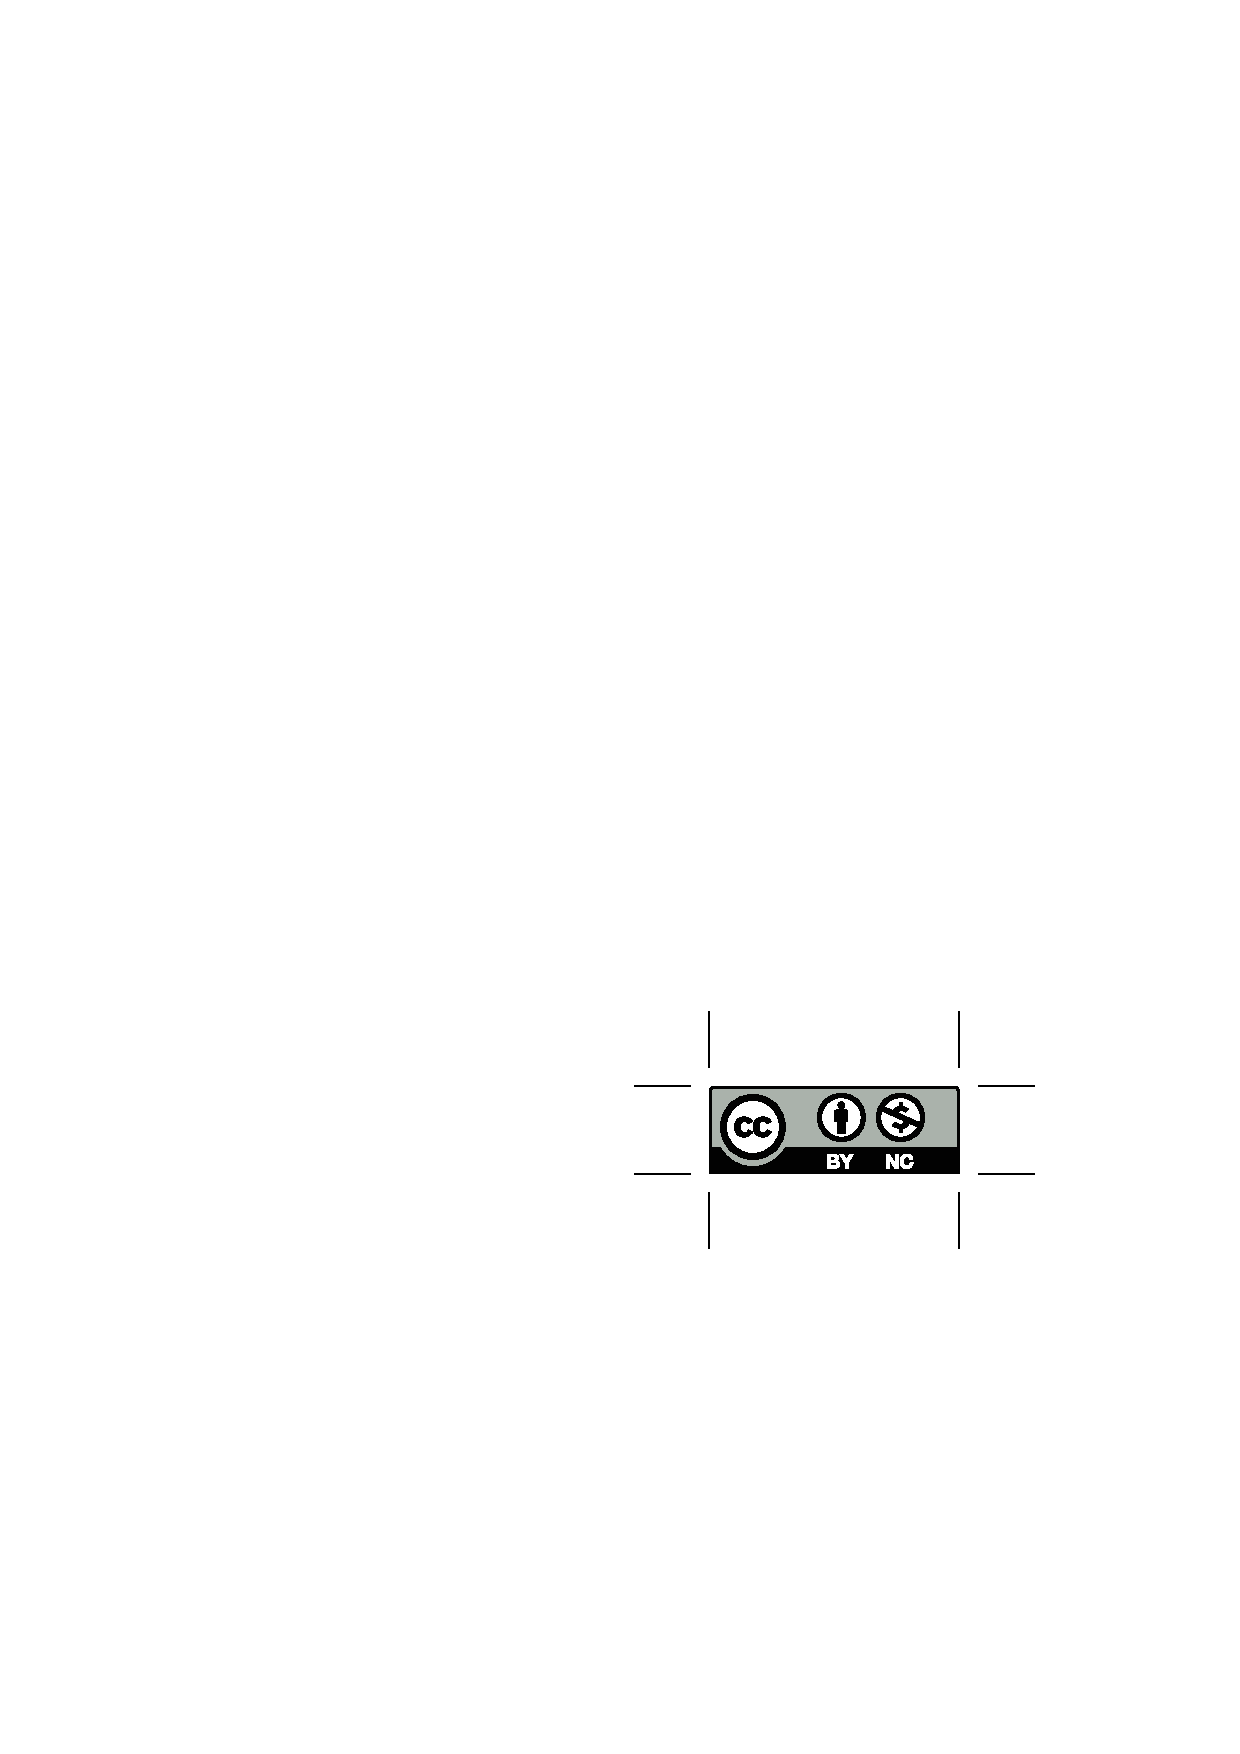
\includegraphics[width=2in]{text/by-nc} 
\end{center}
\end{minipage}
\begin{minipage}{3.3in}
Chapter 3 Copyright \copyright\ 2015 Gregory Hartman

Licensed under the Creative Commons Attribution-Noncommercial 4.0 International Public License
\end{minipage}

\bigskip

\bigskip

\bigskip

\noindent\hskip-1in\begin{minipage}{2.2in}
\begin{center}
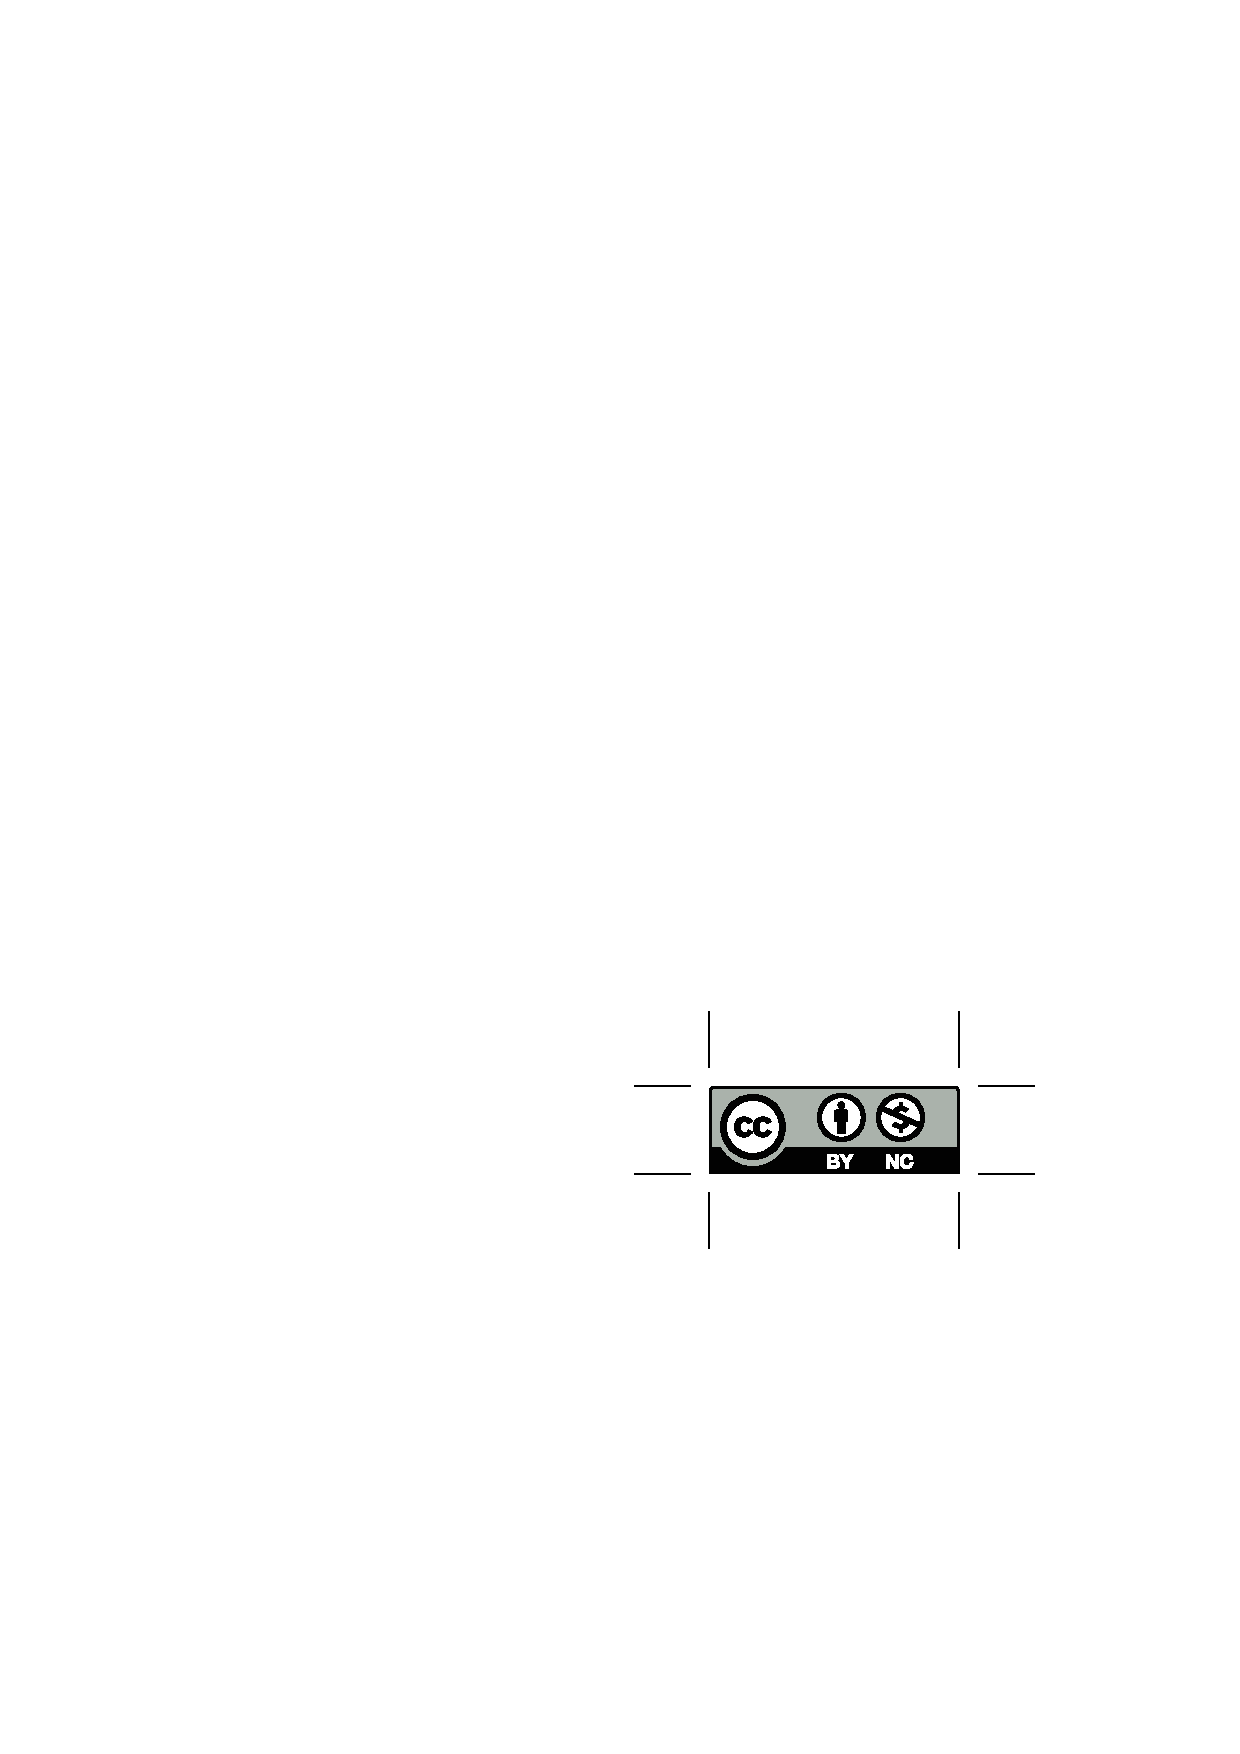
\includegraphics[width=2in]{text/by-nc}
\end{center}
\end{minipage}
\begin{minipage}{3.3in}
Chapters 4-8 Copyright \copyright\ 2011 Gregory Hartman, except as noted below.

Licensed under the Creative Commons Attribution-Noncommercial 3.0 United States License
\end{minipage}

\vspace{1in}


This version of the text was assembled and edited by Sean Fitzpatrick, University of Lethbridge, July-August, 2016. In addition to minor changes and additions throughout the text, supplementary content for this text was written by Sean Fitzpatrick, including all of Section 4.2, and parts of Sections 3.3-3.6, 4.1, 4.5, 6.1, 6.4, 7.4, and 8.1.

\medskip

This work is licensed under the Creative Commons Attribution-Noncommercial-ShareAlike 4.0 International Public License

\vspace{\stretch{1}} 
\thispagestyle{empty}
\clearpage
%
%
%\cleardoublepage
%%%%\phantomsection
%%%%\Huge
\noindent {\bf \textsc{Thanks}}\\

\vspace{1in}
\normalsize

This text took a great deal of effort to accomplish and I owe a great many people thanks. \\
\bigskip

I owe Michelle (and Sydney and Alex) much for their support at home. Michelle puts up with much as I continually read \LaTeX\ manuals, sketch outlines of the text, write exercises, and draw illustrations.\\

My thanks to the Department of Mathematics and Computer Science at Virginia Military Institute for their support of this project. Lee Dewald and Troy Siemers, my department heads, deserve special thanks for their special encouragement and recognition that this effort has been a worthwhile endeavor.\\

My thanks to all who informed me of errors in the text or provided ideas for improvement. Special thanks to Michelle Feole and Dan Joseph who each caught a number of errors.\\

This whole project would have been impossible save for the efforts of the \LaTeX\ community. This text makes use of about 15 different packages, was compiled using MiK\TeX, and edited using \TeX nicCenter, all of which was provided free of charge. This generosity helped convince me that this text should be made freely available as well.

%%%%\addcontentsline{toc}{chapter}{Thanks} 
%%%%\clearpage{\pagestyle{empty}\cleardoublepage}
%%%%\phantomsection
%%%%\thispagestyle{empty}
\Huge
\noindent {\bf \textsc{Preface}}\\
\large
\emph{A Note on Using this Text}
\vspace{1in}
\normalsize

Thank you for reading this short preface. Allow us to share a few key points about the text so that you may better understand what you will find beyond this page.

This text comprises a three--volume series on Calculus. The first part covers material taught in many ``Calc 1'' courses: limits, derivatives, and the basics of integration, found in Chapters 1 through 6.1. The second text covers material often taught in ``Calc 2:'' integration and its applications, along with an introduction to sequences, series and Taylor Polynomials, found in Chapters 5 through 8. The third text covers topics common in ``Calc 3'' or ``multivariable calc:'' parametric equations, polar coordinates, vector--valued functions, and functions of more than one variable, found in Chapters 9 through 13. All three are available separately for free at \texttt{\href{http://apexcalculus.com}{www.apexcalculus.com}}. %These three texts are intended to work together and make one cohesive text, \textit{APEX Calculus}, which can also be downloaded from the website. 

Printing the entire text as one volume makes for a large, heavy, cumbersome book. One can certainly only print the pages they currently need, but some prefer to have a nice, bound copy of the text. Therefore this text has been split into these three manageable parts, each of which can be purchased for under \$15 at \href{http://amazon.com}{Amazon.com}.\\ 



%A result of this splitting is that sometimes a concept is said to be explored in a ``later section,'' though that section does not actually appear in this particular text. Downloading the .pdf of \textit{APEX Calculus} will ensure that you have all the content.  
%material is referenced that is not contained in the present text. The context should make it clear whether the ``missing'' material is in the \textit{Calculus I} or \textit{Calculus III} portion. Downloading the appropriate .pdf, or the whole \textit{APEX Calculus} .pdf, will give access to these topics.
% This splitting of the material also results in unfortunate page/chapter numberings. Chapter 5 of this text is Chapter 1 of \textit{Calculus II}. Apart from these numberings, page--for--page the content of the sections that appear in both \textit{Calculus I} and \textit{Calculus II} are identical.\\ %For instance, in this text, ``Theorem 20'' may be mentioned, although Theorem 20 is only presented in Part I. To minimize confusion, theorems, definitions and key ideas are referenced by their title or subject matter, not their number.

%The current publisher of this text does not allow one text to be split across multiple volumes, with continuity of chapters and page numberings. This is the one drawback of the current publishing model that has many advantages, highlighted below. Because of this, there are a few peculiarities 

\noindent\textbf{\large For Students: How to Read this Text}\\

Mathematics textbooks have a reputation for being hard to read. High--level mathematical writing often seeks to say much with few words, and this style often seeps into texts of lower--level topics. This book was written with the goal of being easier to read than many other calculus textbooks, without becoming too verbose. 

Each chapter and section starts with an introduction of the coming material, hopefully setting the stage for ``why you should care,'' and ends with a look ahead to see how the just--learned material helps address future problems. 

\textit{Please read the text;} it is written to explain the concepts of Calculus. There are numerous examples to demonstrate the meaning of definitions, the truth of theorems, and the application of mathematical techniques. When you encounter a sentence you don't understand, read it again. If it still doesn't make sense, read on anyway, as sometimes confusing sentences are explained by later sentences.

\textit{You don't have to read every equation.} The examples generally show ``all'' the steps needed to solve a problem. Sometimes reading through each step is helpful; sometimes it is confusing. When the steps are illustrating a new technique, one probably should follow each step closely to learn the new technique. When the steps are showing the mathematics needed to find a number to be used later, one can usually skip ahead and see how that number is being used, instead of getting bogged down in reading how the number was found.

\textit{Most proofs have been omitted.} In mathematics, \textit{proving} something is always true is extremely important, and entails much more than testing to see if it works twice. However, students often are confused by the details of a proof, or become concerned that they should have been able to construct this proof on their own. To alleviate this potential problem, we do not include the proofs to most theorems in the text. The interested reader is highly encouraged to find proofs online or from their instructor. In most cases, one is very capable of understanding what a theorem \textit{means} and \textit{how to apply it} without knowing fully \textit{why} it is true.
\\

\thispagestyle{empty}
\noindent\textbf{\large Interactive, 3D Graphics}\\

New to Version 3.0 is the addition of interactive, 3D graphics in the .pdf version. Nearly all graphs of objects in space can be rotated, shifted, and zoomed in/out so the reader can better understand the object illustrated. 

As of this writing, the only pdf viewers that support these 3D graphics are Adobe Reader \& Acrobat (and only the versions for PC/Mac/Unix/Linux computers, not tablets or smartphones). To activate the interactive mode, click on the image. Once activated, one can click/drag to rotate the object and use the scroll wheel on a mouse to zoom in/out. (A great way to investigate an image is to first zoom in on the page of the pdf viewer so the graphic itself takes up much of the screen, then zoom inside the graphic itself.) A CTRL-click/drag pans the object left/right or up/down. By right-clicking on the graph one can access a menu of other options, such as changing the lighting scheme or perspective. One can also revert the graph back to its default view. If you wish to deactive the interactivity, one can right-click and choose the ``Disable Content'' option. \\

\noindent\textbf{\large Thanks}\\

There are many people who deserve recognition for the important role they have played in the development of this text. First, I thank Michelle for her support and encouragement, even as this ``project from work'' occupied my time and attention at home. Many thanks to Troy Siemers, whose most important contributions extend far beyond the sections he wrote or the 227 figures he coded in Asymptote for 3D interaction.  He provided incredible support, advice and encouragement for which I am very grateful. My thanks to Brian Heinold and Dimplekumar Chalishajar for their contributions and to Jennifer Bowen for reading through so much material and providing great feedback early on. Thanks to Troy, Lee Dewald, Dan Joseph, Meagan Herald, Bill Lowe, John David, Vonda Walsh, Geoff Cox, Jessica Libertini and other faculty of VMI who have given me numerous suggestions and corrections based on their experience with teaching from the text. (Special thanks to Troy, Lee \& Dan for their patience in teaching Calc III while I was still writing the Calc III material.) Thanks to Randy Cone for encouraging his tutors of VMI's Open Math Lab to read through the text and check the solutions, and thanks to the tutors for spending their time doing so. A very special thanks to Kristi Brown and Paul Janiczek who took this opportunity far above \& beyond what I expected, meticulously checking every solution and carefully reading every example. Their comments have been extraordinarily helpful. I am also thankful for the support provided by Wane Schneiter, who as my Dean provided me with extra time to work on this project. I am blessed to have so many people give of their time to make this book better.\\

\noindent\textbf{\large \apex\  -- Affordable Print and Electronic teXts}\\

\apex\ is a consortium of authors  who collaborate to produce high--quality, low--cost textbooks. The current textbook--writing paradigm is facing a potential revolution as desktop publishing and electronic formats increase in popularity. However, writing a good textbook is no easy task, as the time requirements alone are substantial. It takes countless hours of work to produce text, write examples and exercises, edit and publish. Through collaboration, however, the cost to any individual can be lessened, allowing us to create texts that we freely distribute electronically and sell in printed form for an incredibly low cost. Having said that, nothing is entirely free; someone always bears some cost. This text ``cost'' the authors of this book their time, and that was not enough. \textit{APEX Calculus} would not exist had not the Virginia Military Institute, through a generous Jackson--Hope grant, given the lead author significant time away from teaching so he could focus on this text.

Each text is available as a free .pdf, protected by a Creative Commons Attribution - Noncommercial 4.0 copyright. That  means you can give the .pdf to anyone you like, print it in any form you like, and even edit the original content and redistribute it. If you do the latter, you must  clearly reference this work and you cannot sell your edited work for money.

We encourage others to adapt this work to fit their own needs. One might add sections that are ``missing'' or remove sections that your students won't need. The source files can be found at \texttt{\href{https://github.com/APEXCalculus}{github.com/APEXCalculus}}.

You can learn more at \texttt{\href{http://www.vmi.edu/APEX}{www.vmi.edu/APEX}}.
\thispagestyle{empty}


%%%%\addcontentsline{toc}{chapter}{Preface}
%%%%\clearpage{\pagestyle{empty}\cleardoublepage}
%%%%\phantomsection
%
% The following is the correct TOC; the 
%
%%%%

\addtocontents{toc}{\protect\thispagestyle{empty}}
\addcontentsline{toc}{chapter}{Table of Contents}
\tableofcontents
\clearpage{\pagestyle{empty}\cleardoublepage}

\phantomsection
\prefacegeometry
\addcontentsline{toc}{chapter}{Preface}
\thispagestyle{empty}
\Huge
\noindent {\bf \textsc{Preface}}\\
\normalsize

This is a textbook on Linear Algebra, designed to be compatible with the curriculum for the course Math 1410 at the University of Lethbridge. As this is a first-year course taken primarily by non-majors, the focus of the text (and the course) is primarily computational, and as a result, much of the theory that common to many first courses in linear algebra is not included.

The book does, however, contain a few topics not always found in a linear algebra course (but required for Math 1410), including vector geometry and complex numbers.

The book is \textit{free}, in every sense of the word. There is no cost to the student, unless one wants a hard copy, in which case the only cost is that of having it printed. The text is also free in less tangible, but equally important ways. The book is licensed under a Creative Commons Public License, which allows you to share the book with others, and even make and distribute copies, as long as this is not done for financial gain. The book is also \textit{open source}: all of the code and figures used to generate the text (over 2,000 files in all) are available online and can be downloaded and edited by anyone wishing to create their own version of the book.

The book has a few quirks compared to other texts. There is an extensive treatment of the arithmetic of complex numbers, since this is required in the Math 1410 course. The treatment of systems of equations also appears quite late in the textbook. In my experience, when the course begins with systems of equations, many students tune out early, either because the material is too easy, or too boring, and aren't able to get back up to speed once the level of difficulty picks up. Having some challenging material early on provides some incentive to do the homework and seek help from the beginning.

Since Math 1410 does not align well with the standard linear algebra curriculum found in many American universities, it was not possible to work with any one pre-existing open textbook. Instead, this book is an amalgamation of three texts, as specified on the copyright page, along with a substantial chunk of content that I've added myself. As a result, you'll find that there are slight differences in the format of some chapters.

The treatment of standard topics like basis and dimension is quite limited, due to the nature of the course. Arguments are provided in support of most theorems in the text, but there aren't too many formal proofs. Some topics that are sometimes taught in Math 1410 also receive a limited treatment here. Eigenvalues and eigenvectors are covered, but diagonalization is not. (Update for the Spring 2017 edition: a section on diagonalization has been added.) The coverage of orthogonality is limited to the shortest distance applications in the chapter on vector geometry. In some cases these omissions are due to time constraints, both in the preparation of the textbook and in the delivery of the material in the classroom. In some cases (such as the Gram-Schmidt procedure and orthogonal diagonalization), there was a concious decision to omit material that more rightly belongs in a second course in linear algebra.

With any luck, the book will continue to evolve as I and other instructors use it. The book is a work in progress, and is bound to have some failings. If you encounter any errors as you use the book (or if you don't like how something is presented, or if you think more exercises of a certain type are needed, etc.) please let me know, and I'll do my best to make the changes. 



\pagebreak

\noindent\textbf{\large Changes in the Spring 2017 edition}

During the inaugural Fall 2016 run for this textbook, I came across a number of errors and typos that have been corrected. Most of these were formatting errors, but there were a few incorrect answers in the back, and one case in Section 6.1 where I somehow used the columns from the wrong matrix in a column space example!

In Chapter 2 I've added formal definitions for addition and multiplication of complex numbers, and the presentation in Section 2.2 has been streamlined. Since the polar coordinate representation of a complex number never has $r<0$, I've removed the material (needed for calculus) involving polar coordinates with $r<0$, as well as the material (also needed for calculus) on converting equations of curves in the plane from rectangular to polar coordinates. Replacing the ``cis'' notation with Euler's exponential notation remains on the to-do list.

In Chapter 3, I've added the standard definition of parallel vectors for linear algebra, and changed the original definition to a theorem. In Chapter 4, I've added additional examples and exercises on span and linear independence in Section 4.2, and two additional examples in Section 4.5 on working with the definition of a linear transformation.

Chapters 5-7 remain largely unchanged, aside from error corrections. In Chapter 8, I've added a new section, on diagonalization. This section introduces the main ideas, such as similar matrices, algebraic and geometric multiplicity, and eigenspaces. There is no treatment of orthogonal diagonalization, since I still consider this topic to be a better fit for Math 3410 than Math 1410.

\bigskip

\bigskip


\noindent\textbf{\large Acknowledgements}\\

First and foremost, I need to thank the authors of the textbooks that provide the source material for this text. Without their hard work, and willingness to make their books (and the source code) freely available, it would not have been possible to create an affordable textbook for this course. You can find the original textbooks at their websites:

\bigskip


\href{http://www.stitz-zeager.com}{www.stitz-zeager.com}, for the \textit{Precalculus} textbook, by Stitz and Zeager, 

\bigskip

\href{http://www.vmi.edu/academics/departments/applied-mathematics/affordable-textbooks-apex/}{http://www.vmi.edu/academics/departments/applied-mathematics/affordable-textbooks-apex/}, for the \textit{Fundamentals of Matrix Algebra} textbook, by Gregory Hartman, and

\bigskip

\href{http://www.apexcalculus.com}{apexcalculus.com}, for the \apex\ \textit{Calculus} textbook, by Hartman et al.



\vspace{1in}

\begin{raggedright}
Sean Fitzpatrick\\
Department of Mathematics and Computer Science\\
University of Lethbridge\\
December 15, 2016
\end{raggedright}





\restoregeometry
\clearpage{\pagestyle{empty}\cleardoublepage}

%%%%%
%\includepdf[pages={1,2}]{CalculusTOC.pdf}

%%%%
\mainmatter


%%%%
%		End block comment here
%%%%







\clearpage{\pagestyle{empty}\cleardoublepage}
\chapter{The Real Numbers}\label{chapter:realnumbers}
\thispagestyle{empty}
This first chapter is intended as a resource for those students needing a quick review of some of the essential high school mathematics for this course. We begin with some basic set theory terminology that may pop up from time to time, followed by a reminder on the rules for arithmetic with real numbers, and a tour of the Cartesian coordinate plane. Students who are already comfortable with these topics can feel free to jump ahead to Chapter 2.

\section{Some Basic Set Theory Notions}
\label{SetTheory}

%\label{SetTheoryNotions}


%\label{SetsofNumbers}

\definition{setdef}{Set}{
A \sword{set}\index{set ! definition of} is a well-defined collection of objects which are called the `elements' of the set.  Here, `well-defined' means that it is possible to determine if something belongs to the collection or not, without prejudice. 
}

\smallskip

For example, the collection of letters that make up the word ``pronghorns'' is well-defined and is a set, but  the collection of the worst math teachers in the world is \textbf{not} well-defined, and so is \textbf{not} a set.  In general, there are three ways to describe sets.  They are

\mnote{.5}{One thing that student evaluations teach us is that any given Mathematics instructor can be simultaneously the best and worst teacher ever, depending on who is completing the evaluation.}

\smallskip

\keyidea{idea:setdescription}{Ways to Describe Sets}{
\begin{enumerate}

\item \textbf{The Verbal Method:} Use a sentence to define a set.\index{set ! verbal description}

\item \textbf{The Roster Method:}  Begin with a left brace `$\{$', list each element of the set \textit{only once} and then end with a right brace `$\}$'.\index{set ! roster method}

\item \textbf{The Set-Builder Method:} A combination of the verbal and roster methods using a ``dummy variable'' such as $x$.\index{set ! set-builder notation}\index{set-builder notation}

\end{enumerate}
}
\smallskip

For example, let $S$ be the set described \textit{verbally} as the set of letters that make up the word ``pronghorns''.  A  \sword{roster} description of $S$ would be  $\left\{ p, r, o, n, g, h, s \right\}$. Note that we listed `r', `o', and `n' only once, even though they appear twice in ``pronghorns.''  Also, the \textit{order} of the elements doesn't matter, so $\left\{ o, n, p, r, g, s, h \right\}$ is also a roster description of $S$.   A \sword{set-builder} description of $S$ is: \[ \{ x \, | \, \mbox{$x$ is a
letter in the word ``pronghorns''.}\} \]

The way to read this is: `The set of elements $x$ \underline{such that} $x$ is a letter in the word ``pronghorns.'''   We define to sets to be equal if they have exactly the same elements, and denote this using the familiar equals sign `$=$'. Thus, we may write
$S = \left\{  p, r, o, n, g, h, s  \right\}$ or  $S = \{ x \, | \, \mbox{$x$ is a
letter in the word ``pronghorns''.}\}$.
Clearly $r$ is an element of $S$ and $q$ is not an element $S$.  We express these sentiments mathematically by writing  $r \in S$ and $q \notin S$. 

More precisely, we have the following.

\medskip

\definition{notationforsetinclusion}{Notation for set inclusion}{ Let $A$ be a set.

\begin{itemize}

\item If $x$ is an element of $A$ then we write $x \in A$\index{set ! inclusion}\index{$\in$} which is read `$x$ is in $A$'.

\item If $x$ is \emph{not} an element of $A$ then we write $x \notin A$\index{set ! exclusion}\index{$\notin$} which is read `$x$ is not in $A$'.

\end{itemize}
}

\mnote{.75}{The notation $x\in A$ can be read as ``$x$ is in $A$'', or ``$x$ is an element of $A$'', or ``$x$ belongs to $A$'', with similar readings for $x\notin A$.}

\medskip

Now let's consider the set 
\[
C =  \{ x \, | \, \mbox{$x$ is a consonant in the word ``pronghorns''}\}.
\]
A roster description of $C$ is  $C = \{ p, r, n, g, h, s\}$.  Note that by construction, every element of $C$ is also in $S$.  We express this relationship by stating that the set $C$ is a \textbf{subset} of the set $S$, which is written in symbols as $C \subseteq S$.  The more formal definition is given below.

\medskip

\definition{subsetdef}{Subset}{
Given sets $A$ and $B$, we say that the set $A$ is a \textbf{subset}\index{subset ! definition of} of the set $B$ and write `$A \subseteq B$' if every element in $A$ is also an element of $B$.  
}

\medskip

Note that in our example above $C \subseteq S$, but not vice-versa, since $o \in S$ but $o \notin C$.  Additionally, the set of vowels $V = \{ a, e, i, o, u\}$, while it does have an element in common with $S$, is not a subset of $S$. (As an added note,  $S$ is not a subset of $V$, either.)  We could, however, \textit{build} a set which contains both $S$ and $V$ as subsets by gathering all of the elements in both $S$ and $V$ together into a single set, say $U = \{ p, r, o, n, g, h, s, a, e, i, u\}$.   Then $S \subseteq U$ and $V \subseteq U$.  The set $U$ we have built is called the \textbf{union} of the sets $S$ and $V$ and is denoted $S \cup V$.    Furthermore, $S$ and $V$ aren't completely \textit{different} sets since they both contain the letter `o.' (Since the word `different' could be ambiguous, mathematicians use the word \textit{disjoint} to refer to two sets that have no elements in common.) The \textbf{intersection} of two sets is the set of elements (if any) the two sets have in common. In this case, the intersection of $S$ and $V$ is $\{ o\}$, written $S \cap V = \{ o \}$.  We formalize these ideas below.

\medskip

\definition{intersectionunion}{Intersection and Union}{
 Suppose $A$ and $B$ are sets.

\begin{itemize}

\item The \textbf{intersection}\index{set ! intersection}\index{intersection of two sets} of $A$ and $B$ is $A \cap B = \{ x \, | \, x \in A \, \text{and} \,\, x \in B \}$

\item The \textbf{union}\index{set ! union}\index{union of two sets} of $A$ and $B$ is $A \cup B = \{ x \, | \, x \in A \, \text{or} \,\, x \in B \, \, \text{(or both)} \}$

\end{itemize}
}

\medskip

The key words in Definition \ref{intersectionunion} to focus on are the conjunctions:  `intersection' corresponds to `and' meaning the elements have to be in \textit{both} sets to be in the intersection, whereas `union' corresponds to `or' meaning the elements have to be in one set, or the other set (or both).  In other words, to belong to the union of two sets an element must belong to \textit{at least one} of them.

\smallskip

Returning to the sets $C$ and $V$  above, $C \cup V = \{ p, r, n, g, h, s, a, e, i, o, u\}$. When it comes to their intersection, however, we run into a bit of notational awkwardness since $C$ and $V$ have no elements in common.  While we could write $C \cap V = \{ \}$, this sort of thing happens often enough that we give the set with no elements a name. 

\medskip

\definition{emptysetdefn}{Empty set}{
The \textbf{Empty Set} $\emptyset$ is the set which contains no elements.\index{set ! empty}\index{empty set}  That is, \[\emptyset=\{ \}=\{x\,|\,\mbox{$x \neq x$}\}.\]  
}

\medskip

As promised, the empty set is the set containing no elements since no matter what `$x$' is, `$x = x$.'  Like the number `$0$,'  the empty set plays a vital role in mathematics. We introduce it here more as a symbol of convenience as opposed to a contrivance.
\mnote{.85}{The full extent of the empty set's role will not be explored in this text, but it is of fundamental importance in Set Theory. In fact, the empty set can be used to generate numbers -  mathematicians can create something from nothing! If you're interested, read about the \href{https://en.wikipedia.org/wiki/Natural_number\#von_Neumann_construction}{von Neumann construction of the natural numbers} or consider signing up for Math 2000.}   
Using this new bit of notation, we have for the sets $C$ and $V$ above that $C \cap V = \emptyset$.    A nice way to visualize relationships between sets and set operations is to draw a  \href{http://en.wikipedia.org/wiki/Venn_diagram}{\underline{\textbf{Venn Diagram}}}\index{diagram ! Venn Diagram}\index{Venn Diagram}.  A Venn Diagram for the sets $S$, $C$ and $V$ is drawn in Figure \ref{venndiagram}.

\mtable{.68}{A Venn diagram for $C$, $S$, and $V$}{venndiagram}{
\myincludegraphics[width=0.95\marginparwidth]{figures/SetTheory-1}
}

In Figure \ref{venndiagram} we have three circles - one for each of the sets $C$, $S$ and $V$.  We visualize the area enclosed by each of these circles as the elements of each set.  Here, we've spelled out the elements for definitiveness.  Notice that the circle representing the set $C$ is completely inside the circle representing $S$.  This is a geometric way of  showing that $C \subseteq S$.  Also, notice that the circles representing $S$ and $V$ overlap on the letter `o'.  This common region is how we visualize $S \cap V$.  Notice that since $C \cap V = \emptyset$, the circles which represent $C$ and $V$ have no overlap whatsoever.  

\medskip

All of these circles lie in a rectangle labelled $U$ (for `universal' set).  A universal set contains all of the elements under discussion, so it could always be taken as the union of all of the sets in question, or an even larger set.  In this case, we could take $U = S \cup V$ or $U$ as the set of letters in the entire alphabet.    The usual triptych of Venn Diagrams indicating generic sets $A$ and  $B$ along with $A \cap B$ and $A \cup B$ is given in Figure \ref{fig:intunion}.

(The reader may well wonder if there is an ultimate universal set which contains \textit{everything}.  The short answer is `no'. Our definition of a set turns out to be overly simplistic, but correcting this takes us well beyond the confines of this course. If you want the longer answer, you can begin by reading about \href{http://en.wikipedia.org/wiki/Russell's_paradox}{\underline{Russell's Paradox}} on Wikipedia.)

\mtable{.32}{Venn diagrams for intersection and union}{fig:intunion}{
\begin{tabular}{c}
\myincludegraphics[scale=0.8]{figures/SetTheory-2}\\
Sets $A$ and $B$.\\
\\
\myincludegraphics[scale=0.8]{figures/SetTheory-3}\\
$A\cap B$ is shaded.\\
\\
\myincludegraphics[scale=0.8]{figures/SetTheory-4}\\
$A\cup B$ is shaded.
\end{tabular}
}



%\pagebreak

In the next section, we will review the algebraic properties of the real number system. Other properties of the real numbers (such as the order property that allows us to picture the set of real numbers as a ``number line'') are essential to Calculus, but not that important for Linear Algebra, so we will leave it to other courses (such as Math 1010 or Math 1560) to handle the discussion of these topics.

\clearpage

\section{Real Number Arithmetic}
\label{RealNumberArithmetic}


In this section we list the properties of real number arithmetic.  This is meant to be a succinct, targeted review so we'll resist the temptation to wax poetic about these axioms and their subtleties and refer the interested reader to a more formal course in Abstract Algebra.  There are two (primary) operations one can perform with real numbers:  addition and multiplication.  

\medskip

\definition{realnumberaddition}{Properties of Real Number Addition}{

\begin{itemize}

\item  \textbf{Closure:}  For all real numbers $a$ and $b$,  $a+b$ is also a real number.

\item  \textbf{Commutativity:}  For all real numbers $a$ and $b$, $a+b = b+a$.

\item  \textbf{Associativity:}  For all real numbers $a$, $b$ and $c$, $a+(b+c) = (a+b)+c$.

\item  \textbf{Identity:}  There is a real number `$0$' so that for all real numbers $a$, $a+0 = a$.

\item  \textbf{Inverse:}  For all real numbers $a$, there is a real number $-a$ such that $a + (-a) = 0$.

\item \textbf{Definition of Subtraction:}  For all real numbers $a$ and $b$, $a - b = a + (-b)$.

\end{itemize}
}

\medskip

Next, we give real number multiplication a similar treatment.  Recall that we may denote the product of two real numbers $a$ and $b$ a variety of ways:  $ab$, $a \cdot b$, $a(b)$, $(a)(b)$ and so on.  We'll refrain from using $a \times b$ for real number multiplication in this text.

\medskip

\definition{realnumbermultiplication}{Properties of Real Number Multiplication}{

\begin{itemize}

\item  \textbf{Closure:}  For all real numbers $a$ and $b$,  $ab$ is also a real number.

\item  \textbf{Commutativity:}  For all real numbers $a$ and $b$, $ab = ba$.

\item  \textbf{Associativity:}  For all real numbers $a$, $b$ and $c$, $a(bc) = (ab)c$.

\item  \textbf{Identity:}  There is a real number `$1$' so that for all real numbers $a$, $a \cdot 1 = a$.

\item  \textbf{Inverse:}  For all real numbers $a \neq 0$, there is a real number $\dfrac{1}{a}$ such that $a \left(\dfrac{1}{a}\right) = 1$.

\item \textbf{Definition of Division:}  For all real numbers $a$ and $b \neq 0$, $a \div b = \dfrac{a}{b} = a  \left(\dfrac{1}{b}\right)$.
\end{itemize}
}

\medskip

While most students (and some faculty) tend to skip over these properties or give them a cursory glance at best, it is important to realize that the properties stated above are what drive the symbolic manipulation for all of Algebra.  When listing a tally of more than two numbers, $1 + 2 + 3$\label{howtoaddonetwothree} for example, we don't need to specify the order in which those numbers are added. Notice though, try as we might, we can add only two numbers at a time and it is the associative property of addition which assures us that we could organize this sum as $(1+2) + 3$ or $1+(2+3)$.  This brings up a note about `grouping symbols'.  Recall that parentheses and brackets are used in order to specify which operations are to be performed first.  In the absence of such grouping symbols, multiplication (and hence division) is given priority over addition (and hence subtraction). For example, $1 + 2 \cdot 3 = 1+6 = 7$, but $(1+2) \cdot 3 = 3 \cdot 3 = 9$.  As you may recall, we can `distribute' the $3$ across the addition if we really wanted to do the multiplication first:  $(1+2) \cdot 3 = 1\cdot 3 + 2 \cdot 3 = 3 + 6 = 9$. More generally, we have the following.

\medskip

\definition{distributiveproperty}{The Distributive Property and Factoring}{
%\smallskip
For all real numbers $a$, $b$ and $c$:

\begin{itemize}

\item  \textbf{Distributive Property:}   $a(b+c) = ab + ac$ and $(a+b)c = ac + bc$.

\item  \textbf{Factoring:}  $ab+ac = a(b+c)$ and $ac + bc = (a+b)c$.

\end{itemize}
}

\medskip

\noindent {\bf Warning:} A common source of errors for beginning students is the misuse (that is, lack of use) of parentheses. When in doubt, more is better than less: redundant parentheses add clutter, but do not change meaning, whereas writing $2x+1$ when you meant to write $2(x+1)$ is almost guaranteed to cause you to make a mistake. (Even if you're able to proceed correctly in spite of your lack of proper notation, this is the sort of thing that will get you on your grader's bad side, so it's probably best to avoid the problem in the first place.)

\medskip


It is worth pointing out that we didn't really need to list the Distributive Property both for $a(b+c)$ (distributing from the left) and $(a+b)c$ (distributing from the right), since the commutative property of multiplication gives us one from the other.  Also, `factoring' really is the same equation as the distributive property, just read from right to left. These are the first of many redundancies in this section, and they exist in this review section for one reason only - in our experience, many students \textit{see} these things differently so we will list them as such.   

\smallskip

It is hard to overstate the importance of the Distributive Property.  For example, in the expression $5(2+x)$, without knowing the value of $x$, we cannot perform the addition inside the parentheses first;  we must rely on the distributive property here to get  $5(2+x) = 5\cdot 2 + 5 \cdot x = 10 + 5x$.  The Distributive Property is also responsible for combining `like terms'.  Why is $3x + 2x = 5x$?  Because  $3x + 2x = (3+2)x = 5x$.  

\smallskip

We continue our review with summaries of other properties of arithmetic, each of which can be derived from the properties listed above.  First up are properties of the additive identity $0$.

\medskip

\theorem{propertiesofzero}{Properties of Zero}{

Suppose $a$ and $b$ are real numbers.

\begin{itemize}

\item  \textbf{Zero Product Property:} $ab = 0$ if and only if $a=0$ or $b=0$ (or both)

\textbf{Note:} This not only says that $0 \cdot a = 0$ for any real number $a$, it also says that the \textit{only} way to get an answer of `$0$' when multiplying two real numbers  is to have one (or both) of the numbers be `$0$' in the first place.

\item  \textbf{Zeros in Fractions:}  If $a \neq 0$, $\dfrac{0}{a} = 0 \cdot \left(\dfrac{1}{a}\right) = 0$.

\textbf{Note:}  The quantity $\dfrac{a}{0}$ is undefined.
\end{itemize}
}

\mnote{.8}{
The Zero Product Property drives most of the equation solving algorithms in Algebra because it allows us to take complicated equations and reduce them to simpler ones.  For example, you may recall that one way to solve  $x^2+x-6=0$ is by factoring the left hand side of this equation to get  $(x-2)(x+3) = 0$.  From here, we apply the Zero Product Property and set each factor equal to zero.  This yields  $x-2=0$ or $x+3=0$ so $x=2$ or $x=-3$.  This type of calculation is key to finding the eigenvalues of a matrix, as we'll see in Section \ref{sec:eigen}.
}


\medskip

We now continue with a review of arithmetic with fractions.


\keyidea{fractionarithmetic}{Properties of Fractions}{
Suppose $a$, $b$, $c$ and $d$ are real numbers.  Assume them to be nonzero whenever necessary; for example,  when they appear in a denominator.

\begin{itemize}

\item  \textbf{Identity Properties:}  $a = \dfrac{a}{1}$ and $\dfrac{a}{a} = 1$.

\item  \textbf{Fraction Equality:}  $\dfrac{a}{b} = \dfrac{c}{d}$ if and only if $ad = bc$. 

\item  \textbf{Multiplication of Fractions:}  $\dfrac{a}{b} \cdot \dfrac{c}{d} = \dfrac{ac}{bd}$. In particular:  $\dfrac{a}{b} \cdot c = \dfrac{a}{b} \cdot \dfrac{c}{1} = \dfrac{ac}{b}$

\mnote{.4}{\textbf{Note:}  A common denominator is \textbf{not} required to \textbf{multiply} or \textbf{divide} fractions!}

\item  \textbf{Division of Fractions:}  $\dfrac{a}{b} \left/ \dfrac{c}{d}\right. = \dfrac{a}{b} \cdot \dfrac{d}{c} = \dfrac{ad}{bc}$. 

In particular: $1 \left/ \dfrac{a}{b}\right. = \dfrac{b}{a}$ and  $\dfrac{a}{b} \left/ c \right. = \dfrac{a}{b} \left/ \dfrac{c}{1}\right.  = \dfrac{a}{b} \cdot \dfrac{1}{c} = \dfrac{a}{bc}$

\mnote{.48}{It's always worth remembering that division is the same as multiplication by the reciprocal. You'd be surprised how often this comes in handy.}

\item  \textbf{Addition and Subtraction of Fractions:}  $\dfrac{a}{b} \pm \dfrac{c}{b} = \dfrac{a \pm c}{b}$.  

\mnote{.36}{\textbf{Note:}  A common denominator \textbf{is} required to \textbf{add or subtract} fractions!}

\item  \textbf{Equivalent Fractions:}  $\dfrac{a}{b} = \dfrac{ad}{bd}$, since $ \dfrac{a}{b} = \dfrac{a}{b} \cdot 1 = \dfrac{a}{b} \cdot \dfrac{d}{d} = \dfrac{ad}{bd}$

\mnote{.28}{\textbf{Note:}  The \textit{only} way to change the denominator is to multiply both it and the numerator by the same nonzero value because we are, in essence, multiplying the fraction by $1$.}

\item  \textbf{`Reducing' Fractions:} $\dfrac{a\cancel{d}}{b\cancel{d}} = \dfrac{a}{b}$, since  $\dfrac{ad}{bd} = \dfrac{a}{b} \cdot \dfrac{d}{d} = \dfrac{a}{b} \cdot 1 = \dfrac{a}{b}$.

In particular, $\dfrac{ab}{b} = a$ since $\dfrac{ab}{b} = \dfrac{ab}{1 \cdot b} =  \dfrac{a \cancel{b}}{1 \cdot \cancel{b}} = \dfrac{a}{1} = a$ and $\dfrac{b-a}{a-b} = \dfrac{(-1)\cancel{(a-b)}}{\cancel{(a-b)}} = -1$.

\mnote{.2}{We reduce fractions by `cancelling' common factors - this is really just reading the previous property `from right to left'.\textbf{Caution:}  We may only cancel common \textbf{factors} from both numerator and denominator.}
\end{itemize}
}

\medskip


Next up is a review of the arithmetic of `negatives'. On page \pageref{realnumberaddition} we first introduced the dash which we all recognize as the `negative' symbol in terms of the additive inverse.  For example, the number $-3$ (read `negative $3$') is defined so that $3 + (-3) = 0$.  We then defined subtraction using the concept of the additive inverse again so that, for example, $5 - 3 = 5 + (-3)$.  



\medskip

\keyidea{propertiesofnegatives}{Properties of Negatives}{
Given real numbers $a$ and $b$ we have the following.  

\begin{itemize}

\item  \textbf{Additive Inverse Properties:}  $-a = (-1)a$ and $-(-a) = a$

\item  \textbf{Products of Negatives:} $(-a)(-b) = ab$. 

\item  \textbf{Negatives and Products:} $-ab = -(ab) = (-a)b = a(-b)$.

\item  \textbf{Negatives and Fractions:} If $b$ is nonzero, $-\dfrac{a}{b} = \dfrac{-a}{b} = \dfrac{a}{-b}$ and $\dfrac{-a}{-b} = \dfrac{a}{b}$.

\item  \textbf{`Distributing' Negatives:}  $-(a+b) = -a-b$ and $-(a-b) = -a + b = b-a$.

\item  \textbf{`Factoring' Negatives:} $-a-b = -(a+b)$ and $b-a = -(a-b)$.

\end{itemize}
}

\mnote{.5}{In this text we do not distinguish typographically between the dashes in the expressions `$5-3$' and `$-3$' even though they are mathematically quite different. In the expression `$5-3$,' the dash is a \textit{binary} operation (that is, an operation requiring \textit{two} numbers) whereas in `$-3$', the dash is a \textit{unary} operation (that is, an operation requiring only one number).  You might ask, `Who cares?'  Your calculator does - that's who!  In the text we can write $-3 - 3 = -6$ but that will not work in your calculator.  Instead you'd need to type $^{-}3 - 3$ to get $-6$ where the first dash comes from the `$+/-$' key.}

\mnote{.8}{
It might be junior high (elementary?) school material, but arithmetic with fractions is one of the most common sources of errors among university students. If you're not comfortable working with fractions, we strongly recommend seeing your instructor (or a tutor) to go over this material until you're completely confident that you understand it. Experience (and even formal educational \href{http://home.isr.umich.edu/releases/fractions-are-the-key-to-math-success-new-study-shows/}{\underline{studies}}) suggest that your success handling fractions corresponds pretty well with your overall success in passing your Mathematics courses.
}

\medskip

An important point here is that when we `distribute' negatives, we do so across addition or subtraction only.  This is because we are really distributing a factor of $-1$ across each of these terms:  $-(a+b) = (-1)(a+b) = (-1)(a) + (-1)(b) = (-a)+(-b) = -a-b$. Negatives do not `distribute' across multiplication:  $- (2 \cdot 3) \neq (-2)\cdot(-3)$. Instead, $-(2\cdot 3) = (-2)\cdot (3) = (2) \cdot (-3) = -6$.  The same sort of thing goes for fractions:  $- \frac{3}{5}$ can be written as $\frac{-3}{5}$ or $\frac{3}{-5}$, but not $\frac{-3}{-5}$.  It's about time we did a few examples to see how these properties work in practice.

\medskip

\example{fractionreview}{Arithmetic with fractions}{
Perform the indicated operations and simplify. By `simplify' here, we mean to have the final answer written in the form $\frac{a}{b}$ where $a$ and $b$ are integers which have no common factors.  Said another way, we want $\frac{a}{b}$ in `lowest terms'.

\begin{multicols}{3}
\begin{enumerate}

\item $\dfrac{1}{4} + \dfrac{6}{7}$\vphantom{$\dfrac{\dfrac{12}{5} - \dfrac{7}{24}}{1 + \left(\dfrac{12}{5}\right) \left(\dfrac{7}{24}\right)}$}
\item $\dfrac{5}{12} - \left(\dfrac{47}{30} - \dfrac{7}{3}\right)$\vphantom{$\dfrac{\dfrac{12}{5} - \dfrac{7}{24}}{1 + \left(\dfrac{12}{5}\right) \left(\dfrac{7}{24}\right)}$}
\item $\dfrac{\dfrac{12}{5} - \dfrac{7}{24}}{1 + \left(\dfrac{12}{5}\right) \left(\dfrac{7}{24}\right)}$ 

\setcounter{HW}{\value{enumi}}
\end{enumerate}
\end{multicols}


\begin{multicols}{2}
\begin{enumerate}
\setcounter{enumi}{\value{HW}}

\item $\dfrac{(2(2)+1)(-3-(-3)) - 5(4-7)}{4-2(3)}$\vphantom{$\left(\dfrac{3}{5} \right) \left(\dfrac{5}{13} \right) - \left(\dfrac{4}{5}\right) \left( - \dfrac{12}{13}\right)$}
\item $\left(\dfrac{3}{5} \right) \left(\dfrac{5}{13} \right) - \left(\dfrac{4}{5}\right) \left( - \dfrac{12}{13}\right)$

\setcounter{HW}{\value{enumi}}
\end{enumerate}
\end{multicols}
}
{
\begin{enumerate}

\item It may seem silly to start with an example this basic but experience has taught us not to take much for granted.  We start by finding the lowest common denominator and then we rewrite the fractions using that new denominator.  Since $4$ and $7$ are {\bf relatively prime},\index{relatively prime} meaning they have no factors in common, the lowest common denominator is $4 \cdot 7 = 28$.\[ \begin{array}{rclr}

\dfrac{1}{4} + \dfrac{6}{7} & = & \dfrac{1}{4} \cdot \dfrac{7}{7} + \dfrac{6}{7} \cdot \dfrac{4}{4} &  \text{Equivalent Fractions} \\ [10pt]
                                           & = & \dfrac{7}{28}  + \dfrac{24}{28} & \text{Multiplication of Fractions}\\ [10pt]
																					 & = & \dfrac{31}{28}                  & \text{Addition of Fractions} \\ \end{array} \]

The result is in lowest terms because $31$ and $28$ are relatively prime so we're done.

%%%%%%%%%%%%%%%%%%%

\mnote{.65}{We could have used $12 \cdot 30 \cdot 3 = 1080$ as our common denominator but then the numerators would become unnecessarily large.  It's best to use the \emph{lowest} common denominator.}

\item  We could begin with the subtraction in parentheses, namely $\frac{47}{30} - \frac{7}{3}$, and then subtract that result from $\frac{5}{12}$.  It's easier, however, to first distribute the negative across the quantity in parentheses and then use the Associative Property to perform all of the addition and subtraction in one step.  The lowest common denominator for all three fractions is $60$.

%\noindent\hskip-50pt
%\begin{minipage}{1.2\linewidth}

\begin{align*}
\dfrac{5}{12} - \left(\dfrac{47}{30} - \dfrac{7}{3}\right) & = \dfrac{5}{12} - \dfrac{47}{30} + \dfrac{7}{3} \quad \tag*{Distribute the Negative}\\ 
& =  \dfrac{5}{12} \cdot \dfrac{5}{5} - \dfrac{47}{30} \cdot \dfrac{2}{2} + \dfrac{7}{3} \cdot \dfrac{20}{20} \quad \tag*{Equivalent Fractions}\\ 
& =  \dfrac{25}{60} - \dfrac{94}{60} + \dfrac{140}{60} \quad \tag*{Multiplication of Fractions} \\
& =  \dfrac{71}{60} \quad \tag*{Addition and Subtraction of Fractions} \\ \end{align*}
%\end{minipage}

\drawexampleline

The numerator and denominator are relatively prime so the fraction is in lowest terms and we have our final answer.

%%%%%%%%%%%%%%%%%%%%%%%%%%%%%%%


\item What we are asked to simplify in this problem is known as a  `complex' or `compound' fraction.  Simply put, we have fractions within a fraction.  The longest division line (also called a `vinculum') acts as a grouping symbol, quite literally dividing the compound fraction into a numerator (containing fractions) and a denominator (which in this case does not contain fractions):

\[
\dfrac{\dfrac{12}{5} - \dfrac{7}{24}}{1 + \left(\dfrac{12}{5}\right) \left(\dfrac{7}{24}\right)} =  \dfrac{\left(\dfrac{12}{5} - \dfrac{7}{24}\right)}{\left(1 + \left(\dfrac{12}{5}\right) \left(\dfrac{7}{24}\right)\right)} 
\] 

The first step to simplifying a compound fraction like this one is to see if you can simplify the little fractions inside it. There are two ways to proceed. One is to simplify the numerator and denominator separately, and then use the fact that division is the same thing as multiplication by the reciprocal, as follows:

\begin{align*}
 \dfrac{\left(\dfrac{12}{5} - \dfrac{7}{24}\right)}{\left(1 + \left(\dfrac{12}{5}\right) \left(\dfrac{7}{24}\right)\right)} & = \dfrac{\left(\dfrac{12}{5}\cdot \dfrac{24}{24} - \dfrac{7}{24}\cdot \dfrac{5}{5}\right)}{\left(1\cdot \dfrac{120}{120} + \left(\dfrac{12}{5}\right) \left(\dfrac{7}{24}\right)\right)} & &\text{Equivalent Fractions}\\ 
& =  \dfrac{288/120 - 35/120}{120/120 + 84/120} & & \text{Multiplication of fractions} \\
& = \dfrac{253/120}{204/120} & & \text{Addition and subtraction of fractions} \\
& = \dfrac{253}{\cancel{120}}\cdot \dfrac{\cancel{120}}{204} & &\text{Division of fractions and cancellation} & &\\
 & =  \dfrac{253}{204} & &
 \end{align*}

 
Since $253 = 11 \cdot 23$ and $204 = 2 \cdot 2 \cdot 3 \cdot 17$ have no common factors our result is in lowest terms which means we are done.


While there is nothing wrong with the above approach, we can also use our Equivalent Fractions property to rid ourselves of the `compound' nature of this fraction straight away.  The idea is to multiply both the numerator and denominator by the lowest common denominator of each of the `smaller' fractions - in this case, $24 \cdot 5 = 120$.

\drawexampleline

\begin{align*}
 \dfrac{\left(\dfrac{12}{5} - \dfrac{7}{24}\right)}{\left(1 + \left(\dfrac{12}{5}\right) \left(\dfrac{7}{24}\right)\right)} & = \dfrac{\left(\dfrac{12}{5} - \dfrac{7}{24}\right) \cdot 120}{\left(1 + \left(\dfrac{12}{5}\right) \left(\dfrac{7}{24}\right)\right) \cdot 120} & & \text{Equivalent Fractions}\\
& =  \dfrac{\left(\dfrac{12}{5}\right) (120) - \left(\dfrac{7}{24}\right) (120)}{(1)(120) + \left(\dfrac{12}{5}\right) \left(\dfrac{7}{24}\right)(120)} & & \text{Distributive Property} \\
& =  \dfrac{\dfrac{12 \cdot 120}{5} - \dfrac{7 \cdot 120}{24}}{120 + \dfrac{12 \cdot 7 \cdot 120}{5 \cdot 24}} & & \text{Multiply fractions} \\
& =  \dfrac{\dfrac{12 \cdot 24 \cdot \cancel{5}}{\cancel{5}} - \dfrac{7 \cdot 5 \cdot \cancel{24}}{\cancel{24}}}{120 + \dfrac{12 \cdot 7 \cdot \cancel{5} \cdot \cancel{24}}{\cancel{5} \cdot \cancel{24}}} & & \text{Factor and cancel} \\
 & =  \dfrac{(12 \cdot 24) - (7 \cdot 5)}{120 + (12 \cdot 7)} & &\\ 
 & =  \dfrac{288 - 35}{120 + 84} =  \dfrac{253}{204}, & & \\
  \end{align*}
which is the same as we obtained above.

%%%%%%%%%%%%%%%%%%%%%%%%%%%%%%%%%%%%%%%%

																					
\item  This fraction may look simpler than the one before it, but the negative signs and parentheses mean that we shouldn't get complacent.  Again we note that the division line here acts as a grouping symbol.  That is, 

\[ \dfrac{(2(2)+1)(-3-(-3)) - 5(4-7)}{4-2(3)} = \dfrac{\left((2(2)+1)(-3-(-3)) - 5(4-7) \right)}{(4-2(3))} \]

This means that we should simplify the numerator and denominator first, then perform the division last.  We tend to what's in parentheses first, giving multiplication priority over addition and subtraction.
\begin{align*}
\dfrac{(2(2)+1)(-3-(-3)) - 5(4-7)}{4-2(3)} & =  \dfrac{(4+1)(-3+3)-5(-3)}{4 - 6}   \\ 
                                           & =  \dfrac{(5)(0) + 15}{-2}   \\ 
																					 & =  \dfrac{15}{-2}  \\ 
																					 & =  -\dfrac{15}{2}  \tag*{Properties of Negatives}
																					 \end{align*}
Since $15 = 3\cdot 5$ and $2$ have no common factors, we are done.
																			

%%%%%%%%%%%%%%%%%%%%%%%%%%%%%%


\item  In this problem, we have multiplication and subtraction.  Multiplication takes precedence so we perform it first.  Recall that to multiply fractions, we do \textit{not} need to obtain common denominators;  rather, we multiply the corresponding numerators together along with the corresponding denominators.  Like the previous example, we have parentheses and negative signs for added fun!
\begin{align*}
\left(\dfrac{3}{5} \right) \left(\dfrac{5}{13} \right) - \left(\dfrac{4}{5}\right) \left( - \dfrac{12}{13}\right) & =  \dfrac{3 \cdot 5}{5 \cdot 13} - \dfrac{4\cdot (-12)}{5 \cdot 13}  \tag*{Multiply fractions}\\ 
& =  \dfrac{15}{65} - \dfrac{-48}{65}  \\
& =  \dfrac{15}{65} + \dfrac{48}{65}  \tag*{Properties of Negatives}\\
& =  \dfrac{15+48}{65}   \tag*{Add numerators} \\ 
& =  \dfrac{63}{65}  \\
\end{align*}

Since $64 = 3 \cdot 3 \cdot 7$ and $65 = 5 \cdot 13$ have no common factors, our answer $\dfrac{63}{65}$ is in lowest terms and we are done.
\end{enumerate}
} 

\medskip

Of the issues discussed in the previous set of examples none causes students more trouble than simplifying compound fractions.  We presented two different methods for simplifying them:  one in which we simplified the overall numerator and denominator and then performed the division and one in which we removed the compound nature of the fraction at the very beginning.   We encourage the reader to go back and use both methods on each of the compound fractions presented.  Keep in mind that when a compound fraction is encountered in the rest of the text it will usually be simplified using only one method and we may not choose your favourite method.  Feel free to use the other one in your notes.

\smallskip

Next, we review exponents and their properties.  Recall that $2 \cdot 2 \cdot 2$  can be written as $2^3$ because exponential notation expresses repeated multiplication.  In the expression $2^3$, $2$ is called the \textbf{base}\index{base} and $3$ is called the \textbf{exponent}\index{exponent}. In order to generalize exponents from natural numbers to the integers, and eventually to rational and real numbers, it is helpful to think of the exponent as a count of the number of factors of the base we are multiplying by $1$.  For instance, \[2^3 = 1 \cdot (\text{three factors of two}) = 1 \cdot (2 \cdot 2 \cdot 2) = 8.\] From this, it makes sense that \[2^{0} = 1 \cdot (\text{zero factors of two}) = 1.\]  What about $2^{-3}$?  The `$-$' in the exponent indicates that we are `taking away' three factors of two, essentially dividing by three factors of two.  So, \[2^{-3} = 1 \div (\text{three factors of two}) = 1 \div (2 \cdot 2 \cdot 2) = \frac{1}{2 \cdot 2 \cdot 2} = \frac{1}{8}.\]  We summarize the properties of integer exponents below.

\medskip

\definition{propertiesofintegerexponents}{Properties of Integer Exponents}{
Suppose $a$ and $b$ are nonzero real numbers and $n$ and $m$ are integers.

\begin{itemize}

\item  \textbf{Product Rules:} $(ab)^{n} = a^n b^n$ and $a^n a^m = a^{n+m}$.

\item  \textbf{Quotient Rules:} $\left(\dfrac{a}{b}\right)^n = \dfrac{a^n}{b^n}$ and $\dfrac{a^n}{a^m} = a^{n-m}$. 

\item \textbf{Power Rule:}  $\left(a^{n}\right)^{m} = a^{nm}$.

\item  \textbf{Negatives in Exponents:}  $a^{-n} = \dfrac{1}{a^n}$.

 In particular, $\left(\dfrac{a}{b}\right)^{-n} = \left(\dfrac{b}{a}\right)^{n} = \dfrac{b^n}{a^n}$ and $\dfrac{1}{a^{-n}} = a^{n}$.

\item  \textbf{Zero Powers:}  $a^{0} = 1$.

\mnote{.35}{Note:  The expression $0^{0}$ is an indeterminate form. See the comment regarding `$\frac{0}{0}$' on page \pageref{propertiesofzero}.}

\item  \textbf{Powers of Zero:}  For any \textit{natural} number $n$, $0^{n} = 0$.

\textbf{Note:}  The expression $0^{n}$ for integers $n \leq 0$ is not defined.

\end{itemize}
}

While it is important the state the Properties of Exponents, it is also equally important to take a moment to discuss one of the most common errors in Algebra.  It is true that $(ab)^2 = a^2 b^2$ (which some students refer to as `distributing' the exponent to each factor) but you {\bf cannot} do this sort of thing with addition.  That is, in general,   $(a+b)^2 \neq a^2 + b^2$. (For example, take $a= 3$ and $b = 4$.)  The same goes for any other powers.

\smallskip

With exponents now in the mix, we can now state the Order of Operations Agreement.

\medskip

\definition{orderofoperations}{Order of Operations Agreement}{
When evaluating an expression involving real numbers:

\begin{enumerate}

\item  Evaluate any expressions in \textbf{p}arentheses (or other grouping symbols.)
\item  Evaluate \textbf{e}xponents.
\item  Evaluate \textbf{d}ivision and \textbf{m}ultiplication as you read from left to right.
\item  Evaluate \textbf{a}ddition and \textbf{s}ubtraction as you read from left to right.

\end{enumerate}
}

\mnote{.3}{Order of operations follows the  ``PEDMAS'' rule some of you may have encountered.}

\medskip

For example, $2 + 3\cdot 4^2 = 2 + 3\cdot 16 = 2 + 48 = 50$.  Where students get into trouble is with things like $-3^2$.  If we think of this as $0 - 3^2$, then it is clear that we evaluate the exponent first:  $-3^2 =0 -3^2 =0 -9 = -9$.  In general, we interpret $-a^n = -\left(a^n\right)$.  If we want the `negative' to also be raised to a power, we must  write $(-a)^n$ instead.  To summarize, $-3^2 = -9$ but $(-3)^2  = 9$. 

\smallskip

Of course, many of the `properties' we've stated in this section can be viewed as ways to circumvent the order of operations. We've already seen how the distributive property allows us to simplify $5(2+x)$ by performing the indicated multiplication \textbf{before} the addition that's in parentheses.  Similarly, consider trying to evaluate $2^{30172}\cdot 2^{-30169}$.  The Order of Operations Agreement demands that the exponents be dealt with first, however, trying to compute $2^{30172}$ is a challenge, even for a calculator.  One of the Product Rules of Exponents, however, allow us to rewrite this product, essentially performing the multiplication first, to get:  $2^{30172-30169} = 2^{3} = 8$.  

\medskip


\example{exponentreview}{Operations with exponents}{
Perform the indicated operations and simplify.

\begin{multicols}{2}

\begin{enumerate}

\item  $\dfrac{(4-2)(2 \cdot 4)-(4)^2}{(4-2)^2}$

\item $12(-5)(-5+3)^{-4}+6(-5)^2(-4)(-5+3)^{-5}$\vphantom{$\dfrac{(4-2)(2 \cdot 4)-(4)^2}{(4-2)^2}$}

\setcounter{HW}{\value{enumi}}

\end{enumerate}

\end{multicols}

\begin{multicols}{2}

\begin{enumerate}

\setcounter{enumi}{\value{HW}}

\item  $\dfrac{\left(\dfrac{5\cdot 3^{51}}{4^{36}}\right)}{\left(\dfrac{5 \cdot 3^{49}}{4^{34}}\right)}$

\item $\dfrac{2 \left(\dfrac{5}{12}\right)^{-1}}{1 - \left(\dfrac{5}{12}\right)^{-2}}$\vphantom{$\dfrac{\left(\dfrac{5\cdot 3^{51}}{4^{36}}\right)}{\left(\dfrac{5 \cdot 3^{49}}{4^{34}}\right)}$}

\end{enumerate}

\end{multicols}
}
{
\begin{enumerate}

\item  We begin working inside parentheses then deal with the exponents before working through the other operations.  As we saw in Example \ref{fractionreview}, the division here acts as a grouping symbol, so we save the division to the end.\[ \begin{array}{rclcl}

\dfrac{(4-2)(2 \cdot 4)-(4)^2}{(4-2)^2} & = & \dfrac{(2)(8)-(4)^2}{(2)^2} & = & \dfrac{(2)(8)-16}{4} \\ [10pt]
                                        & = & \dfrac{16-16}{4} = \dfrac{0}{4} & = & 0 \\ \end{array}\]

\item  As before, we simplify what's in the parentheses first, then work our way through the exponents, multiplication, and finally, the addition.
\begin{align*}
12(-5)(-5+3)^{-4}+6(-5)^2&(-4)(-5+3)^{-5}\\
&  =  12(-5)(-2)^{-4} + 6(-5)^{2}(-4)(-2)^{-5} \\ 
                                         & =  12(-5)\left(\dfrac{1}{(-2)^4}\right) + 6(-5)^{2}(-4)\left(\dfrac{1}{(-2)^5}\right) \\                                         
                                         & =  12(-5)\left(\dfrac{1}{16}\right) + 6(25)(-4)\left(\dfrac{1}{-32}\right) \\
& =  (-60)\left(\dfrac{1}{16}\right) + (-600)\left(\dfrac{1}{-32}\right) \\
& =  \dfrac{-60}{16} + \left(\dfrac{-600}{-32}\right)  \\
& =  \dfrac{-15\cdot \cancel{4}}{4 \cdot \cancel{4}} + \dfrac{-75 \cdot \cancel{8}}{-4 \cdot \cancel{8}}  \\
		& =  \dfrac{-15}{4} + \dfrac{-75}{-4}  \\
			& =  \dfrac{-15}{4} + \dfrac{75}{4}  \\
				& =  \dfrac{-15 + 75}{4}  \\
				& =  \dfrac{60}{4}  \\
	       & =  15  
\end{align*}

\drawexampleline

\item  The Order of Operations Agreement mandates that we work within each set of parentheses first, giving precedence to the exponents, then the multiplication, and, finally the division.  The trouble with this approach is that the exponents are so large that computation becomes a trifle unwieldy.   What we observe, however, is that the bases of the exponential expressions, $3$ and $4$, occur in both the numerator and denominator of the compound fraction, giving us hope that we can use some of the Properties of Exponents (the Quotient Rule, in particular) to help us out. Our first step here is to invert and multiply.  We see immediately that the $5$'s cancel after which we group the powers of $3$ together and the powers of $4$ together and apply the properties of exponents.
\[ \begin{array}{rclclcl}

\dfrac{\left(\dfrac{5\cdot 3^{51}}{4^{36}}\right)}{\left(\dfrac{5 \cdot 3^{49}}{4^{34}}\right)} & = & \dfrac{5\cdot 3^{51}}{4^{36}} \cdot \dfrac{4^{34}}{5 \cdot 3^{49}} & = & \dfrac{\cancel{5} \cdot 3^{51} \cdot 4^{34}}{\cancel{5} \cdot 3^{49} \cdot 4^{36}} & = & \dfrac{3^{51}}{3^{49}} \cdot\dfrac{4^{34}}{4^{36}} \\

& = & 3^{51-49} \cdot 4^{34-36} & = & 3^{2} \cdot 4^{-2} & = & 3^{2} \cdot \left( \dfrac{1}{4^2}\right) \\

& = & 9 \cdot \left(\dfrac{1}{16} \right) & = & \dfrac{9}{16} & & \\ \end{array} \]

\item We have yet another instance of a compound fraction so our first order of business is to rid ourselves of the compound nature of the fraction like we did in Example \ref{fractionreview}.  To do this, however, we need to tend to the exponents first so that we can determine what common denominator is needed to simplify the fraction.
\begin{align*}
\dfrac{2 \left(\dfrac{5}{12}\right)^{-1}}{1 - \left(\dfrac{5}{12}\right)^{-2}} & =  \dfrac{2 \left(\dfrac{12}{5}\right)}{1 - \left(\dfrac{12}{5}\right)^{2}} =  \dfrac{\left(\dfrac{24}{5}\right)}{1 - \left(\dfrac{12^2}{5^2}\right)}\\
 & =  \dfrac{\left(\dfrac{24}{5}\right)}{1 - \left(\dfrac{144}{25}\right)}  =  \dfrac{\left(\dfrac{24}{5}\right) \cdot 25}{\left(1 - \dfrac{144}{25}\right)\cdot 25}\\
  & =  \dfrac{\left(\dfrac{24\cdot 5 \cdot \cancel{5}}{\cancel{5}}\right)}{\left(1 \cdot 25 - \dfrac{144 \cdot \cancel{25}}{\cancel{25}}\right)}  =  \dfrac{120}{25-144} \\
& =  \dfrac{120}{-119} = -\dfrac{120}{119}
\end{align*}
Since $120$ and $119$ have no common factors, we are done. 

\end{enumerate}
}

\medskip

We close our review of real number arithmetic with a discussion of roots and radical notation.  Just as subtraction and division were defined in terms of the inverse of addition and multiplication, respectively, we define roots by undoing natural number exponents.

\medskip


\definition{principalnthrootdefn}{The principal $n^{\text{th}}$ root}{
Let $a$ be a real number and let $n$ be a natural number.  If $n$ is odd, then the \index{$n^{\text{th}}$ root ! principal}\index{principal $n^{\text{th}}$ root}\textbf{principal \boldmath $n^{\textbf{th}}$ root} of $a$ (denoted $\sqrt[n]{a}$) is the unique real number satisfying $\left(\sqrt[n]{a}\right)^n = a$.  If $n$ is even, $\sqrt[n]{a}$ is defined similarly provided  $a \geq 0$ and $\sqrt[n]{a} \geq 0$.  The number $n$ is called the \index{root ! index}\index{index of a root}\textbf{index} of the root and the the number $a$ is called the \index{root ! radicand}\index{radicand}\textbf{radicand}.  For $n=2$, we write $\sqrt{a}$ instead of $\sqrt[2]{a}$.
}


\medskip

The reasons for the added stipulations for even-indexed roots in Definition \ref{principalnthrootdefn} can be found in the Properties of Negatives.  First, for all real numbers,  $x^{\text{even power}} \geq 0$, which means it is never negative.  Thus if $a$ is a \textit{negative} real number, there are no real numbers $x$ with $x^{\text{even power}} = a$.  This is why if $n$ is even, $\sqrt[n]{a}$ only exists if $a \geq 0$.  The second restriction for even-indexed roots is that $\sqrt[n]{a} \geq 0$.  This comes from the fact that $x^{\text{even power}} = (-x)^{\text{even power}}$, and we require $\sqrt[n]{a}$ to have just one value.  So even though $2^{4} = 16$ and $(-2)^{4} = 16$, we require $\sqrt[4]{16} = 2$ and ignore $-2$.  

\smallskip

Dealing with odd powers is much easier. For example, $x^3 = -8$ has one and only one real solution, namely $x = -2$, which means not only does $\sqrt[3]{-8}$ exist, there is only one choice, namely $\sqrt[3]{-8} = -2$. Of course, when it comes to solving $x^{5213} = -117$, it's not so clear that there is one and only one real solution, let alone that the solution is $\sqrt[5213]{-117}$. 

\mnote{.7}{
It's important that you understand the difference between the statements $y=\sqrt{x}$ and $y^2=x$. The equation $y=\sqrt{x}$ defines $y$ as a \textbf{function} of $x$, which means that for each value of $x\geq 0$ there is \text{only one} value of $y$ such that $y=\sqrt{x}$. For example, $y=\sqrt{4}$ is equivalent to $y=2$. On the other hand, there are \textbf{two} solutions to $y^2=x$; namely, $y=\sqrt{x}$ and $y=-\sqrt{x}$. For example, the equation $y^2=4$ is equivalent to the two equations $y=2$ and $y=-2$ (or, more concisely, $y=\pm 2$). Since these two equations are closely related, it's easy to mix them up. The main thing to remember is that $\sqrt{x}$ always denotes the {\em positive} square root of $x$.
}

\smallskip

We list properties of radicals below as a `theorem' since they can be justified using the properties of exponents.

\medskip

\theorem{radicalprops}{Properties of Radicals}{
Let $a$ and $b$ be real numbers and let $m$ and $n$ be natural numbers.  If $\sqrt[n]{a}$ and $\sqrt[n]{b}$ are real numbers, then\index{radical ! properties of}

\begin{itemize}

\item  \textbf{Product Rule:}  $\sqrt[n]{ab} = \sqrt[n]{a} \, \sqrt[n]{b}$ \index{product rule ! for radicals}

\item  \textbf{Quotient Rule:}  $\sqrt[n]{\dfrac{a}{b}} = \dfrac{\sqrt[n]{a}}{\sqrt[n]{b}}$, provided $b \neq 0$. \index{quotient rule ! for radicals}

\item  \textbf{Power Rule:} $\sqrt[n]{a^m} = \left(\sqrt[n]{a}\right)^m$ \index{power rule ! for radicals}

\end{itemize}
}

\medskip

The proof of Theorem \ref{radicalprops} is based on the definition of the principal $n^{\textbf{th}}$ root and the Properties of Exponents.  To establish the product rule, consider the following.  If $n$ is odd, then by definition $\sqrt[n]{ab}$ is the \underline{unique} real number such that $(\sqrt[n]{ab})^{n} = ab$.  Given that $( \sqrt[n]{a} \, \sqrt[n]{b})^n = (\sqrt[n]{a})^n (\sqrt[n]{b})^n = ab$ as well, it must be the case that $\sqrt[n]{ab} = \sqrt[n]{a} \, \sqrt[n]{b}$. If $n$ is even, then $\sqrt[n]{ab}$ is the unique non-negative real number such that $(\sqrt[n]{ab})^{n} = ab$.  Note that since $n$ is even, $\sqrt[n]{a}$ and $\sqrt[n]{b}$ are also non-negative thus $\sqrt[n]{a}\sqrt[n]{b} \geq 0$ as well.  Proceeding as above, we find that $\sqrt[n]{ab} = \sqrt[n]{a} \, \sqrt[n]{b}$.  The quotient rule is proved similarly and is left as an exercise.  The power rule results from repeated application of the product rule, so long as $\sqrt[n]{a}$ is a real number to start with. We leave that as an exercise as well.

\smallskip

We pause here to point out one of the most common errors students make when working with radicals.  Obviously $\sqrt{9} = 3$, $\sqrt{16} = 4$ and $\sqrt{9 + 16} = \sqrt{25} = 5$.  Thus we can clearly see that $5 = \sqrt{25} = \sqrt{9 + 16} \neq \sqrt{9} + \sqrt{16} = 3 + 4 = 7$ because we all know that $5 \neq 7$.  The authors urge you to \textbf{never consider `distributing' roots or exponents}.  It's wrong and no good will come of it because in general $\sqrt[n]{a+b} \neq \sqrt[n]{a} + \sqrt[n]{b}$. 

\phantomsection
\label{donotdistributeexponents}

\smallskip

Since radicals have properties inherited from exponents, they are often written as such.  We define rational exponents in terms of radicals in the box below.

\medskip

\definition{rationalexponentdefn}{Rational exponents}{
Let $a$ be a real number, let $m$ be an integer and let $n$ be a natural number. \index{rational exponent}

\begin{itemize}

\item  $a^{\frac{1}{n}} = \sqrt[n]{a}$ whenever $\sqrt[n]{a}$ is a real number. (If $n$ is even we need $a \geq 0$.)

\item  $a^{\frac{m}{n}}  = \left(\sqrt[n]{a}\right)^m = \sqrt[n]{a^m}$ whenever $\sqrt[n]{a}$ is a real number.

\end{itemize}
}

\medskip

It would make life really nice if the rational exponents defined in Definition \ref{rationalexponentdefn} had all of the same properties that integer exponents have as listed on page \pageref{propertiesofintegerexponents}  - but they don't.  Why not?  Let's look at an example to see what goes wrong.  Consider the Product Rule which says that $(ab)^{n} = a^{n}b^{n}$ and let $a = -16$, $b = -81$ and $n = \frac{1}{4}$.  Plugging the values into the Product Rule yields the equation $((-16)(-81))^{1/4} = (-16)^{1/4}(-81)^{1/4}$.  The left side of this equation is $1296^{1/4}$ which equals $6$ but the right side is undefined because neither root is a real number.  Would it help if, when it comes to even roots (as signified by even denominators in the fractional exponents), we ensure that everything they apply to is non-negative?  That works for some of the rules - we leave it as an exercise to see which ones - but does not work for the Power Rule.

\smallskip
 
Consider the expression $\left(a^{2/3}\right)^{3/2}$.  Applying the usual laws of exponents, we'd be tempted to simplify this as $\left(a^{2/3}\right)^{3/2} = a^{\frac{2}{3} \cdot \frac{3}{2}} = a^{1} = a$.  However, if we substitute $a=-1$ and apply Definition \ref{rationalexponentdefn}, we find $(-1)^{2/3} = \left(\sqrt[3]{-1}\right)^2 = (-1)^2 = 1$ so that $\left((-1)^{2/3}\right)^{3/2} = 1^{3/2} = \left(\sqrt{1}\right)^3 = 1^3 = 1$.  Thus in this case we have $\left(a^{2/3}\right)^{3/2} \neq a$ even though all of the roots were defined.  It is true, however, that $\left(a^{3/2}\right)^{2/3} = a$  and we leave this for the reader to show.  The moral of the story is that when simplifying powers of rational exponents where the base is negative or worse, unknown, it's usually best to rewrite them as radicals.

\medskip

\example{ex_combineop}{Combining operations}{
Perform the indicated operations and simplify. 

  
\begin{enumerate}

\item  $\dfrac{-(-4) - \sqrt{(-4)^2-4(2)(-3)}}{2(2)}$\vphantom{$\dfrac{2 \left( \dfrac{\sqrt{3}}{3}\right)}{1 - \left( \dfrac{\sqrt{3}}{3} \right)^2}$}

\item  $\dfrac{2 \left( \dfrac{\sqrt{3}}{3}\right)}{1 - \left( \dfrac{\sqrt{3}}{3} \right)^2}$



\item  $(\sqrt[3]{-2} - \sqrt[3]{-54})^2$\vphantom{ $2 \left(\dfrac{9}{4} - 3\right)^{1/3} + 2\left(\dfrac{9}{4}\right)\left(\dfrac{1}{3}\right)\left(\dfrac{9}{4}-3\right)^{-2/3}$}

\item  $2 \left(\dfrac{9}{4} - 3\right)^{1/3} + 2\left(\dfrac{9}{4}\right)\left(\dfrac{1}{3}\right)\left(\dfrac{9}{4}-3\right)^{-2/3}$

\end{enumerate}
}
{
\begin{enumerate}

\item  We begin in the numerator and note that the radical here acts a grouping symbol,  so our first order of business is to simplify the radicand. (The line extending horizontally from the square root symbol `$\sqrt{\vphantom{2}}$ is, you guessed it, another vinculum.)

\[ \begin{array}{rclr}

\dfrac{-(-4) -\sqrt{(-4)^2-4(2)(-3)}}{2(2)}  & = & \dfrac{-(-4) - \sqrt{16-4(2)(-3)}}{2(2)} & \\[8pt]
                                             & = & \dfrac{-(-4) - \sqrt{16-4(-6)}}{2(2)} & \\[8pt]
																						& = & \dfrac{-(-4) - \sqrt{16-(-24)}}{2(2)} & \\[8pt]
				                                     & = & \dfrac{-(-4) - \sqrt{16+24}}{2(2)} & \\[8pt]
																						    & = & \dfrac{-(-4) - \sqrt{40}}{2(2)} & \\ \end{array} \] As you may recall, $40$ can be factored using a perfect square as $40 = 4 \cdot 10$ so we use the product rule of radicals to write $\sqrt{40} = \sqrt{4 \cdot 10} = \sqrt{4} \sqrt{10} = 2 \sqrt{10}$.  This lets us factor a `$2$' out of both terms in the numerator, eventually allowing us to cancel it with a factor of $2$ in the denominator.\[ \begin{array}{rclcl}

 \dfrac{-(-4) - \sqrt{40}}{2(2)} & = &  \dfrac{-(-4) - 2\sqrt{10}}{2(2)} & = &  \dfrac{4  - 2\sqrt{10}}{2(2)} \\ [8pt]
                                 & = &  \dfrac{2 \cdot 2  - 2\sqrt{10}}{2(2)} & = &  \dfrac{2(2  - \sqrt{10})}{2(2)} \\ [8pt]
																& = &  \dfrac{\cancel{2}(2  - \sqrt{10})}{\cancel{2}(2)} & = &  \dfrac{2  - \sqrt{10}}{2} \\ \end{array} \]Since the numerator and denominator have no more common factors, we are done. (Do you see why we aren't `cancelling' the remaining $2$'s?)

\item  Once again we have a compound fraction, so we first simplify the exponent in the denominator to see which factor we'll need to multiply by in order to clean up the fraction.\[ \begin{array}{rclcl}

\dfrac{2 \left( \dfrac{\sqrt{3}}{3}\right)}{1 - \left( \dfrac{\sqrt{3}}{3} \right)^2} & = & \dfrac{2 \left( \dfrac{\sqrt{3}}{3}\right)}{1 - \left( \dfrac{(\sqrt{3})^2}{3^2} \right)} & = & \dfrac{2 \left( \dfrac{\sqrt{3}}{3}\right)}{1 - \left( \dfrac{3}{9} \right)}\\ [20pt]
																				
& = & \dfrac{2 \left( \dfrac{\sqrt{3}}{3}\right)}{1 - \left( \dfrac{1 \cdot \cancel{3}}{3 \cdot \cancel{3}} \right)} & = & \dfrac{2 \left( \dfrac{\sqrt{3}}{3}\right)}{1 - \left( \dfrac{1}{3} \right)} \\[20pt]
																
& = & \dfrac{2 \left( \dfrac{\sqrt{3}}{3}\right) \cdot 3}{\left(1 - \left( \dfrac{1}{3} \right)\right) \cdot 3} & = & \dfrac{\dfrac{2 \cdot \sqrt{3} \cdot \cancel{3}}{\cancel{3}}}{1\cdot 3 -  \dfrac{1\cdot \cancel{3}}{\cancel{3}}} \\[20pt]

& = & \dfrac{2 \sqrt{3}}{3 - 1} & = & \dfrac{\cancel{2} \sqrt{3}}{\cancel{2}} = \sqrt{3} \\ \end{array} \]

\drawexampleline

\item  Working inside the parentheses, we first encounter $\sqrt[3]{-2}$.  While the $-2$ isn't a perfect cube, (of an integer, that is!) we may think of $-2 = (-1)(2)$.  Since $(-1)^3 = -1$, $-1$ \textit{is} a perfect cube, and we may write $\sqrt[3]{-2} = \sqrt[3]{(-1)(2)} = \sqrt[3]{-1} \sqrt[3]{2} = - \sqrt[3]{2}$. When it comes to $\sqrt[3]{54}$, we may write it as $\sqrt[3]{(-27)(2)} = \sqrt[3]{-27} \sqrt[3]{2} = -3 \sqrt[3]{2}$.  So, \[\sqrt[3]{-2} - \sqrt[3]{-54} = -\sqrt[3]{2} - (-3\sqrt[3]{2}) = -\sqrt[3]{2} + 3 \sqrt[3]{2}.\]  At this stage, we can simplify $-\sqrt[3]{2} + 3 \sqrt[3]{2} = 2 \sqrt[3]{2}$.  You may remember this as being called `combining like radicals,' but it is in fact just another application of the distributive property:  \[-\sqrt[3]{2} + 3\sqrt[3]{2} = (-1)\sqrt[3]{2} + 3 \sqrt[3]{2} = (-1+3)\sqrt[3]{2} = 2\sqrt[3]{2}.\]  Putting all this together, we get:\[ \begin{array}{rclcl}
  (\sqrt[3]{-2} - \sqrt[3]{-54})^2 & = & (-\sqrt[3]{2} + 3 \sqrt[3]{2})^2 & = & (2 \sqrt[3]{2})^2  \\ [5pt]
																	 & = & 2^2 (\sqrt[3]{2})^2 = 4 \sqrt[3]{2^2} & = & 4 \sqrt[3]{4} \\ \end{array} \] Since there are no perfect integer cubes which are factors of $4$ (apart from $1$, of course), we are done.

%\pagebreak

\item  We start working in parentheses and get a common denominator to subtract the fractions:\[ \dfrac{9}{4} - 3 = \dfrac{9}{4} - \dfrac{3 \cdot 4}{1 \cdot 4} = \dfrac{9}{4} - \dfrac{12}{4} = \dfrac{-3}{4}  \] Since the denominators in the fractional exponents are odd, we can proceed using the properties of exponents:
\begin{align*}
2 \left(\dfrac{9}{4} - 3\right)^{1/3} + 2\left(\dfrac{9}{4}\right)\left(\dfrac{1}{3}\right)&\left(\dfrac{9}{4}-3\right)^{-2/3}  \\
&= 2 \left(\dfrac{-3}{4} \right)^{1/3} + 2\left(\dfrac{9}{4}\right)\left(\dfrac{1}{3}\right)\left(\dfrac{-3}{4}\right)^{-2/3}  \\ 
& =  2 \left(\dfrac{(-3)^{1/3}}{(4)^{1/3}} \right) + 2\left(\dfrac{9}{4}\right)\left(\dfrac{1}{3}\right)\left(\dfrac{4}{-3}\right)^{2/3}  \\ 
& =  2 \left(\dfrac{(-3)^{1/3}}{(4)^{1/3}} \right) + 2\left(\dfrac{9}{4}\right)\left(\dfrac{1}{3}\right)\left(\dfrac{(4)^{2/3}}{(-3)^{2/3}}\right)\\ 
& =  \dfrac{2 \cdot (-3)^{1/3}}{4^{1/3}} + \dfrac{2 \cdot 9 \cdot 1 \cdot 4^{2/3}}{4 \cdot 3 \cdot (-3)^{2/3}}  \\
& = \dfrac{2 \cdot (-3)^{1/3}}{4^{1/3}} + \dfrac{\cancel{2} \cdot 3 \cdot \cancel{3} \cdot 4^{2/3}}{2 \cdot \cancel{2} \cdot \cancel{3} \cdot (-3)^{2/3}} \\ 
& =  \dfrac{2 \cdot (-3)^{1/3}}{4^{1/3}} + \dfrac{3 \cdot 4^{2/3}}{2 \cdot (-3)^{2/3}} 
\end{align*}
At this point, we could start looking for common denominators but it turns out that these fractions reduce even further.  Since $4 = 2^2$, $4^{1/3} = (2^2)^{1/3} = 2^{2/3}$.  Similarly, $4^{2/3} = (2^2)^{2/3} = 2^{4/3}$. The expressions $(-3)^{1/3}$ and $(-3)^{2/3}$ contain negative bases so we proceed with caution and convert them back to radical notation to get:  $(-3)^{1/3} = \sqrt[3]{-3} = -\sqrt[3]{3} = - 3^{1/3}$ and  $(-3)^{2/3} = (\sqrt[3]{-3})^2 = (-\sqrt[3]{3})^2 =(\sqrt[3]{3})^2 = 3^{2/3}$.  Hence:
\begin{align*}
\dfrac{2 \cdot (-3)^{1/3}}{4^{1/3}} + \dfrac{3 \cdot 4^{2/3}}{2 \cdot (-3)^{2/3}} & =  \dfrac{2 \cdot (-3^{1/3})}{2^{2/3}} + \dfrac{3 \cdot 2^{4/3}}{2 \cdot 3^{2/3}}  \\
& =  \dfrac{2^{1} \cdot (-3^{1/3})}{2^{2/3}} + \dfrac{3^{1} \cdot 2^{4/3}}{2^{1} \cdot 3^{2/3}}   \\
& =  2^{1 - 2/3} \cdot (-3^{1/3}) +3^{1- 2/3} \cdot 2^{4/3 - 1}   \\
& =  2^{1/3} \cdot (-3^{1/3}) +3^{1/3} \cdot 2^{1/3}   \\
& =   - 2^{1/3} \cdot 3^{1/3} +3^{1/3} \cdot 2^{1/3}   \\
& =  0 
\end{align*}
\end{enumerate}
}

\printexercises{exercises/00_02_exercises}

\section{The Cartesian Coordinate Plane}
\label{CartesianPlane}

As a warm-up for the discussions of vectors and three-dimensional geometry yet to come, we will make a quick review of the \index{Cartesian coordinate plane} \sword{Cartesian Coordinate Plane}. 
Imagine two real number lines crossing at a right angle at $0$ as shown in Figure \ref{fig:cartplane}.

\mnote{.5}{The Cartesian Plane is named in honour of \href{http://en.wikipedia.org/wiki/Descartes}{\underline{Ren\'{e} Descartes}}.} 



\mfigure[width=0.95\marginparwidth]{.75}{The Cartesian coordinate plane}{fig:cartplane}{figures/CartesianPlane-21}


The horizontal number line is usually called the \index{$x$-axis} \sword{\boldmath $x$-axis} while the vertical number line is usually called the \index{$y$-axis} \sword{\boldmath $y$-axis}.  As with the usual number line, we imagine these axes extending off indefinitely in both directions.   Having two number lines allows us to locate the positions of points off of the number lines as well as points on the lines themselves.  

\mnote{.6}{Usually extending off  towards infinity is indicated by arrows, but here, the arrows are used to indicate the \textit{direction} of increasing values of $x$ and $y$.}

\mnote{.4}{The names of the coordinates can vary depending on the context of the application.  If, for example, the horizontal axis represented time we might choose to call it the $t$-axis.  The first number in the ordered pair would then be the $t$-coordinate.}

\medskip

For example, consider the point $P$ on the next page.  To use the numbers on the axes to label this point, we imagine dropping a vertical line from the $x$-axis to $P$ and extending a horizontal line from the $y$-axis to $P$.  This process is sometimes called `projecting' the point $P$ to the $x$- (respectively $y$-) axis.  We then describe the point $P$ using the \index{ordered pair} \sword{ordered pair} $(2,-4)$.  The first number in the ordered pair is called the \index{abscissa} \sword{abscissa} or \index{$x$-coordinate} \sword{\boldmath $x$-coordinate} and the second is called the \index{ordinate} \sword{ordinate} or \index{$y$-coordinate} \sword{\boldmath $y$-coordinate}.  Taken together, the ordered pair $(2,-4)$ comprise the \index{coordinates ! Cartesian}\index{Cartesian coordinates}\sword{Cartesian coordinates} of the point $P$. In practice, the distinction between a point and its coordinates is blurred; for example, we often speak of `the point $(2,-4)$.'  We can think of $(2,-4)$ as instructions on how to reach $P$ from the \index{origin} {\bf origin} $(0, 0)$ by moving $2$ units to the right and $4$ units downwards.  Notice that the order in the \underline{ordered} pair is important $-$ if we wish to plot the point $(-4,2)$, we would move to the left $4$ units from the origin and then move upwards $2$ units, as below on the right.


\medskip

\noindent\ifthenelse{\isodd{\thepage}}{}{\hskip-110pt}
\noindent\begin{minipage}{1.3\linewidth}
\begin{tabular}{cc}
\myincludegraphics{figures/CartesianPlane-22} &

\myincludegraphics{figures/CartesianPlane-23}\\

\end{tabular}
\end{minipage}



When we speak of the Cartesian Coordinate Plane, we mean the set of all possible ordered pairs $(x,y)$ as $x$ and $y$ take values from the real numbers.  Below is a summary of important facts about Cartesian coordinates.


\smallskip 

\keyidea{idea:cartfacts}{Important Facts about the Cartesian Coordinate Plane}{
\begin{itemize}

\item $(a,b)$ and $(c,d)$ represent the same point in the plane if and only if $a = c$ and $b = d$.

\item  $(x,y)$ lies on the $x$-axis if and only if $y = 0$.

\item  $(x,y)$ lies on the $y$-axis if and only if $x=0$.

\item The origin is the point $(0,0)$.  It is the only point common to both axes.

%\smallskip

\end{itemize}
}

\mnote{.65}{Cartesian coordinates are sometimes referred to as \textit{rectangular coordinates}, to distinguish them from other coordinate systems such as \textit{polar coordinates}: see Section \ref{IntroPolar}. }

\mnote{.55}{We will also see in Chapter \ref{chapter:complex} that the best way to visualize the set of \textit{complex numbers} is by identifying complex numbers with points in the Cartesian plane.}




\mnote{.75}{The letter $O$ is almost always reserved for the origin.}
\example{ex_cartplot}{Plotting points in the Cartesian Plane}{
Plot the following points: $A(5,8)$, $B\left(-\frac{5}{2}, 3\right)$, $C(-5.8, -3)$, $D(4.5, -1)$, $E(5,0)$, $F(0,5)$, $G(-7,0)$, $H(0, -9)$, $O(0,0)$.
}
{
To plot these points, we start at the origin and move to the right if the $x$-coordinate is positive; to the left if it is negative.   Next, we move up if the $y$-coordinate is positive or down if it is negative.  If the $x$-coordinate is $0$, we start at the origin and move along the $y$-axis only.  If the  $y$-coordinate is $0$ we move along the $x$-axis only.


\begin{center}

\myincludegraphics{figures/CartesianPlane-24}

\end{center}
}

\medskip

\pagebreak

The axes divide the plane into four regions called \index{quadrants} \sword{quadrants}.  They are labelled with Roman numerals and proceed counterclockwise around the plane: see Figure \ref{quadrant}.


\mtable{.75}{The four quadrants of the Cartesian plane}{quadrant}{
\begin{tabular}{c}
\myincludegraphics[scale=0.9]{figures/CartesianPlane-25}
\end{tabular}
}

For example, $(1,2)$ lies in Quadrant I, $(-1,2)$ in Quadrant II, $(-1,-2)$ in Quadrant III and $(1,-2)$ in Quadrant IV.  If a point other than the origin happens to lie on the axes, we typically refer to that point as lying on the positive or negative $x$-axis (if $y = 0$) or on the positive or negative $y$-axis (if $x = 0$).  For example, $(0,4)$ lies on the positive $y$-axis whereas $(-117,0)$ lies on the negative $x$-axis.  Such points do not belong to any of the four quadrants.

\smallskip


\subsection{Distance in the Plane}

Another important concept in Geometry is the notion of length.  If we are going to unite Algebra and Geometry using the Cartesian Plane, then we need to develop an algebraic understanding of what distance in the plane means.  Suppose we have two points, $P\left(x_{0}, y_{0}\right)$ and $Q\left(x_{1}, y_{1}\right),$ in the plane. By the \index{distance ! definition} \sword{distance} $d$  between $P$ and $Q$, we mean the length of the line segment joining $P$ with $Q$.  (Remember, given any two distinct points in the plane, there is a unique line containing both points.)  Our goal now is to create an algebraic formula to compute the distance between these two points. Consider the generic situation in Figure \ref{fig:cartdist}(a).

\medskip

\mtable{.45}{Distance between $P$ and $Q$}{fig:cartdist}{
\begin{tabular}{c}
\myincludegraphics{figures/CartesianPlane-28} \\
(a)\\
\\
\myincludegraphics{figures/CartesianPlane-29}\\
(b)
\end{tabular}
}

\medskip

With a little more imagination, we can envision a right triangle whose hypotenuse has length $d$ as drawn in Figure \ref{fig:cartdist}(b).  From the latter figure, we see that the lengths of the legs of the triangle are $\left\lvert x_{1} - x_{0}\right\rvert$ and $\left\lvert y_{1} - y_{0}\right\rvert$ so the \href{http://en.wikipedia.org/wiki/Pythagorean_Theorem}{\underline{Pythagorean Theorem}} gives us
 
  \begin{align*}
   \left\lvert x_{1} - x_{0}\right\rvert^2 + \left\lvert y_{1} - y_{0}\right\rvert^2 &= d^2\\
   \left(x_{1} - x_{0}\right)^2 + \left(y_{1} - y_{0}\right)^2 &= d^2
  \end{align*}
 
\mnote{.2}{Recall that the \sword{absolute value} \index{absolute value} of a real number $a$, denoted by $\abs{a}$, measures the distance of $a$ from the origin. Since we never want a negative distance, this means $\abs{a}=a$ if $a\geq 0$, while if $a<0$, $\abs{a}=-a$. For example, $\abs{4}=4$, and $\abs{-7} = -(-7)= 7$. Given two real numbers $a$ and $b$, $\abs{a-b}$ measures the distance between them.}

(Since the square of a number is always positive, we can drop the absolute value signs.) By extracting the square root of both sides of the second equation and using the fact that distance is never negative, we get
 
\medskip
 
\keyidea{distanceformula}{The Distance Formula}{
\index{distance ! distance formula}  The distance $d$ between the points $P\left(x_{0}, y_{0}\right)$ and $Q\left(x_{1}, y_{1}\right)$ is:
 
\[d = \sqrt{ \left(x_{1} - x_{0}\right)^2 + \left(y_{1} - y_{0}\right)^2} \]
}

\medskip

It is not always the case that the points $P$ and $Q$ lend themselves to constructing such a triangle.  If the points $P$ and $Q$ are arranged vertically or horizontally, or describe the exact same point, we cannot use the above geometric argument to derive the distance formula.  It is left to the reader in Exercise \ref{distanceothercases} to verify Equation \ref{distanceformula} for these cases.

\pagebreak

\example{ex_twoptdist}{Distance between two points}{
Find and simplify the distance between $P(-2,3)$ and  $Q(1,-3)$.  
}
{
\begin{align*}
 d & =  \sqrt{\left(x_{1} - x_{0} \right)^2 + \left(y_{1} - y_{0} \right)^2} \\
   & =  \sqrt{ (1-(-2))^2 + (-3-3)^2} \\
   & =  \sqrt{9 + 36} \\
   & =  3 \sqrt{5}
\end{align*}

So the distance is $3 \sqrt{5}$. 
}

\medskip

\example{ex_pointwithdist}{Finding points at a given distance}{
Find all of the points with $x$-coordinate $1$ which are $4$ units from the point $(3,2)$.
}
{
We shall soon see that the points we wish to find are on the line $x=1$, but for now we'll just view them as points of the form $(1,y)$.  

We require that the distance from $(3,2)$ to $(1,y)$ be $4$.  The Distance Formula, Equation \ref{distanceformula}, yields

\begin{align*} 
d &  =  \sqrt{\left(x_{1}-x_{0}\right)^2+\left(y_{1}-y_{0}\right)^2} \\
4 &  =  \sqrt{(1-3)^2+(y-2)^2}  \\
4  & =  \sqrt{4+(y-2)^2}  \\ 
4^2 & =  \left(\sqrt{4+(y-2)^2}\right)^2   \tag*{squaring both sides} \\
16 & =  4+(y-2)^2 \\
12 & =  (y-2)^2  \\
(y-2)^2 & =  12   \\
y - 2 & =  \pm \sqrt{12} \tag*{extracting the square root} \\
y-2 & =  \pm 2 \sqrt{3}  \\
y & =  2 \pm 2 \sqrt{3}   
\end{align*}


We obtain two answers:  $(1, 2 + 2 \sqrt{3})$ and $(1, 2-2 \sqrt{3}).$  The reader is encouraged to think about why there are two answers.}

\mtable{.5}{Diagram for Example \ref{ex_pointwithdist}}{fig:pointdist}{
\begin{tabular}{c}
\myincludegraphics{figures/CartesianPlane-30}
\end{tabular}
}

\medskip

Related to finding the distance between two points is the problem of finding the \index{midpoint ! definition of} \sword{midpoint} of the line segment connecting two points.  Given two points, $P\left(x_{0}, y_{0}\right)$ and $Q\left(x_{1}, y_{1}\right)$, the \textbf{midpoint} $M$  of $P$ and $Q$ is defined to be the point on the line segment connecting $P$ and $Q$ whose distance from $P$ is equal to its distance from  $Q$.  

\mtable{.16}{The midpoint of a line segment}{fig:midptseg}{
\begin{tabular}{c}
\myincludegraphics{figures/CartesianPlane-31}
\end{tabular}
}

If we think of reaching $M$ by going `halfway over' and `halfway up' we get the following formula. 

\medskip

\keyidea{midpointformula}{The Midpoint Formula}{
\index{midpoint ! midpoint formula}The midpoint $M$ of the line segment connecting $P\left(x_{0}, y_{0}\right)$ and $Q\left(x_{1}, y_{1}\right)$  is:

\[ 
M = \left( \dfrac{x_{0} + x_{1}}{2} , \dfrac{y_{0} + y_{1}}{2} \right)
\]
}

\medskip

If we let $d$ denote the distance between $P$ and $Q$, we leave it as Exercise \ref{verifymidpointformula} to show that the distance between $P$ and $M$ is $d/2$ which is the same as the distance between $M$ and $Q$.  This suffices to show that Key Idea \ref{midpointformula} gives the coordinates of the midpoint.

\medskip

\example{ex_findmidpoint}{Finding the midpoint of a line segment}
{
Find the midpoint of the line segment connecting $P(-2,3)$ and  $Q(1,-3)$.  
}
{
\begin{align*}
 M & = \left( \dfrac{x_{0}+x_{1}}{2},  \dfrac{y_{0}+y_{1}}{2} \right) \\
   & = \left( \dfrac{(-2)+1}{2},  \dfrac{3+(-3)}{2} \right)  = \left(- \dfrac{1}{2}, \dfrac{0}{2} \right) \\
   & = \left(- \dfrac{1}{2}, 0 \right) 
\end{align*}
The midpoint is  $\left(- \frac{1}{2}, 0 \right)$.}

\medskip

\phantomsection

\label{inversemidpoint}

We close with a more abstract application of the Midpoint Formula.  

\medskip

\example{inversemidpointex1}{An abstract midpoint problem}
{
If $a \neq b$, prove that the line $y = x$ equally divides the line segment with endpoints $(a,b)$ and $(b,a)$.
}
{
To prove the claim, we use Equation \ref{midpointformula} to find the midpoint  

%\setlength{\extrarowheight}{10pt}

\begin{align*}
 M & =  \left( \dfrac{a+b}{2},  \dfrac{b+a}{2} \right) \\
   & =  \left( \dfrac{a+b}{2},  \dfrac{a+b}{2} \right)
\end{align*}

Since the $x$ and $y$ coordinates of this point are the same, we find that the midpoint lies on the line $y=x$, as required. 
}

%\setlength{\extrarowheight}{2pt}
%\closegraphsfile
\printexercises{exercises/00_03_exercises}


\clearpage{\pagestyle{empty}\cleardoublepage}
\chapter{The Complex Numbers}\label{chapter:complex}
\thispagestyle{empty}
\section{Complex Numbers}
\label{CmpNums}

We now move on to the study of the set of \sword{complex numbers}\index{numbers ! complex}\index{complex numbers}.  As you may recall, the complex numbers fill an algebraic gap left by the real numbers.  There is no real number $x$ with $x^2 = -1$, since for any real number $x^2 \geq 0$.  However, we could formally extract square roots and write $x = \pm \sqrt{-1}$.  We build the complex numbers by relabelling the quantity $\sqrt{-1}$ as $i$, the unfortunately misnamed \index{imaginary unit, $i$}\index{complex number ! imaginary unit, $i$}\sword{imaginary unit}.  The number $i$, while not a real number, is defined so that it plays along well with real numbers and acts very much like any other radical expression.  For instance, $3(2i) = 6i$, $7i-3i = 4i$, $(2-7i) + (3 + 4i) = 5-3i$, and so forth.  The key properties which distinguish $i$ from the real numbers are listed below.

\mnote{.7}{Historically, the lack of solutions to the equation $x^2=-1$ had nothing to do with the development of the complex numbers. Until the 19th century, equations such as $x^2=-1$ would have been considered in the context of the analytic geometry of Descartes. The lack of solutions simply indicated that the graph $y=x^2$ did not intersect the line $y=-1$. The more remarkable case was that of \textit{cubic} equations, of the form $x^3=ax+b$. In this case a \textbf{real} solution is \textit{guaranteed}, but there are cases where one needs \textbf{complex} numbers to find it! For details, see the excellent book \textit{Visual Complex Analysis}, by Tristan Needham.}

\medskip

\definition{idefn}{The imaginary unit}{
The imaginary unit $i$ satisfies the two following properties:

\begin{enumerate}

\item  $i^2 = -1$

\item  If $c$ is a real number with $c \geq 0$ then $\sqrt{-c} = i \sqrt{c}$

\end{enumerate}
}

\medskip

\mnote{.55}{Note the use of the indefinite article `a'.  Whatever beast is chosen to be $i$, $-i$ is the other square root of $-1$.}

\mnote{.45}{Some Technical Mathematics textbooks label the imaginary unit `$j$', usually to avoid confusion with the use of the letter $i$ to denote electric current.  While it carries the adjective `imaginary', these numbers have essential real-world implications.  For example, every electronic device owes its existence to the study of `imaginary' numbers.}

Property 1 in Definition \ref{idefn} establishes that $i$ does act as a square root of $-1$, and property 2 establishes what we mean by the `principal square root' of a negative real number.  In property 2, it is important to remember the restriction on $c$.  For example, it is perfectly acceptable to say  $\sqrt{-4} = i \sqrt{4} = i(2) = 2i$. However, $\sqrt{-(-4)} \neq i \sqrt{-4}$, otherwise, we'd get\[ 2 = \sqrt{4} = \sqrt{-(-4)} = i \sqrt{-4} = i (2i) = 2i^2 = 2(-1) = -2,\] which is unacceptable. The moral of this story is that the general properties of radicals do not apply for even roots of negative quantities.  With Definition \ref{idefn} in place, we are now in position to define the \index{complex number ! definition of}\sword{complex numbers}.

\medskip

\definition{complexdefn}{Complex number}{
A \sword{complex number} is a number of the form $a+bi$, where $a$ and $b$ are real numbers and $i$ is the imaginary unit.  The set of complex numbers is denoted $\C$.
}

\medskip

Complex numbers include things you'd normally expect, like $3+2i$ and $\frac{2}{5} - i\sqrt{3}$.  However, don't forget that $a$ or $b$ could be zero, which means numbers like $3i$ and $6$ are also complex numbers.  In other words, don't forget that the complex numbers \textit{include} the real numbers, so $0$ and $\pi - \sqrt{21}$ are both considered complex numbers.   The arithmetic of complex numbers is as you would expect.  The only things you need to remember are the two properties in Definition \ref{idefn}.  The next example should help recall how these animals behave.

\mnote{.3}{To use the language  of Section \ref{SetsofNumbers}, $\R \subseteq \C$.}



\medskip

%\label{complexnumberarithmetic}

\example{complexzeroex1}{Arithmetic with complex numbers}{
Perform the indicated operations.


\begin{multicols}{3}
\begin{enumerate}

\item  $(1-2i) - (3+4i)$ \vphantom{$\dfrac{1-2i}{3-4i}$}
\item  $(1-2i)(3+4i)$ \vphantom{$\dfrac{1-2i}{3-4i}$}
\item  $\dfrac{1-2i}{3-4i}$

\setcounter{HW}{\value{enumi}}
\end{enumerate}
\end{multicols}

\begin{multicols}{3}
\begin{enumerate}
\setcounter{enumi}{\value{HW}}

\item  $\sqrt{-3} \sqrt{-12}$
\item  $\sqrt{(-3)(-12)}$
\item  $(x-[1+2i])(x-[1-2i])$

\setcounter{HW}{\value{enumi}}
\end{enumerate}
\end{multicols}
}
{
\begin{enumerate}

\item  As mentioned earlier, we treat expressions involving $i$ as we would any other radical. We distribute and combine like terms:
\begin{align*}
 (1-2i) - (3+4i) & =   1-2i-3-4i  \tag*{Distribute} \\
                 & =   -2 - 6i  \tag*{Gather like terms} \\
\end{align*}
Technically, we'd have to rewrite our answer  $-2-6i$ as $(-2) + (-6)i$ to be (in the strictest sense) `in the form $a+bi$'. That being said, even pedants have their limits, and we'll consider $-2-6i$ good enough.

\item  Using the Distributive Property (a.k.a. F.O.I.L.), we get
\begin{align*}
  (1-2i)(3+4i)  & =  (1)(3) + (1)(4i) - (2i)(3) - (2i)(4i)  \tag*{F.O.I.L.} \\
	              & =  3+4i-6i-8i^2  \\
								& =  3 - 2i - 8(-1)  \tag*{$i^2=-1$} \\
								& =  3 - 2i + 8  \\
								& =  11 - 2i 
\end{align*}

\drawexampleline

\item  How in the world are we supposed to simplify $\frac{1-2i}{3-4i}$?  Well, we deal with the denominator $3-4i$ as we would any other denominator containing two terms, one of which is a square root: we and multiply both numerator and denominator by $3+4i$, the (complex) conjugate of $3 - 4i$.  Doing so produces\\begin{align*}
 \dfrac{1-2i}{3-4i} & =  \dfrac{(1-2i)(3+4i)}{(3-4i)(3+4i)}  \tag*{Equivalent Fractions} \\[5pt]
                    & =    \dfrac{3 + 4i - 6i - 8i^2}{9 - 16i^2}  \tag*{F.O.I.L.}\\[5pt]
					& =  \dfrac{3 - 2i - 8(-1)}{9  - 16(-1)}  \tag*{$i^2 = -1$}\\[5pt]
					& =  \dfrac{11 - 2i}{25} \\[5pt]
					& =  \dfrac{11}{25} - \dfrac{2}{25} \, i 
\end{align*}
										

\item  We use property 2 of Definition \ref{idefn} first, then apply the rules of radicals applicable to real numbers to get $\sqrt{-3} \sqrt{-12} = \left(i \sqrt{3}\right) \left(i \sqrt{12}\right) = i^2 \sqrt{3\cdot 12} = -\sqrt{36} = -6$.

\item  We adhere to the order of operations here and perform the multiplication before the radical to get  $\sqrt{(-3)(-12)} = \sqrt{36} = 6$. 

\item  We can brute force multiply using the distributive property and see that 
\begin{align*}
(x-[1+2i])(x-[1-2i]) & =  x^2 -x[1-2i]-x[1+2i]+[1-2i][1+2i]  \\
					 & =  x^2-x+2ix-x-2ix+1-2i+2i-4i^2   \\
					 & =  x^2-2x + 1-4(-1) \\
					 & =  x^2 -2x +5 
\end{align*}
\end{enumerate}
}

\medskip

In the previous example, we used the idea of a `conjugate' to divide two complex numbers. (You may recall using conjugates to rationalize expressions involving square roots.)  More generally, the \index{complex number ! complex conjugate ! definition of}\index{conjugate ! complex conjugate ! definition of}\sword{complex conjugate} of a complex number $a+bi$ is the number $a-bi$.  The notation commonly used for complex conjugation is a `bar':  $\overline{a+bi} = a-bi$. For example, $\overline{3+2i} = 3-2i$ and $\overline{3-2i} = 3+2i$. To find $\overline{6}$, we note that $\overline{6} = \overline{6+0i}= 6 - 0i = 6$, so $\overline{6} = 6$. Similarly, $\overline{4i} = -4i$, since $\overline{4i} = \overline{0 + 4i} = 0 - 4i =  -4i$.  Note that $\overline{3+\sqrt{5}} = 3 + \sqrt{5}$, not $3 - \sqrt{5}$, since  $\overline{3+\sqrt{5}} = \overline{3+\sqrt{5} + 0i} = 3+\sqrt{5}  - 0i = 3+\sqrt{5}$. Here, the conjugation specified by the `bar' notation involves reversing the sign before $i = \sqrt{-1}$, not before  $\sqrt{5}$.  The properties of the conjugate are summarized in the following theorem.

\medskip

\theorem{conjugateprops}{Properties of the Complex Conjugate}{
\index{complex number ! conjugate ! properties of}\index{conjugate of a complex number ! properties of}
Let $z$ and $w$ be complex numbers. 

\begin{itemize}

\item  $\overline{\overline{z}} = z$

\item  $ \overline{z+w} = \overline{z} + \overline{w}$

\item  $ \overline{zw} = \overline{z} \, \overline{w}$

\item  $\overline{z^{n}} = \left(\overline{z}\right)^n$, for any natural number $n$

\item  $z$ is a real number if and only if $\overline{z} = z$.

\end{itemize}
}

\medskip

Essentially, Theorem \ref{conjugateprops} says that complex conjugation works well with addition, multiplication and powers.  The proofs of these properties can best be achieved by writing out $z = a+bi$ and $w = c+di$ for real numbers $a$, $b$, $c$ and $d$.   Next, we compute the left and right sides of each equation and verify that they are the same.  

\smallskip

The proof of the first property is a very quick exercise.  To prove the second property, we compare $\overline{z+w}$ with $\overline{z} + \overline{w}$.  We have $\overline{z} + \overline{w} = \overline{a+bi} + \overline{c+di}  = a-bi + c-di$.  To find $\overline{z+w}$, we first compute \[z+w = (a+bi) + (c+di) = (a+c)+(b+d)i\] so \[\overline{z+w} = \overline{(a+c)+(b+d)i} = (a+c) - (b+d)i = a - bi + c - di = \overline{z} + \overline{w}\]  As such, we have established  $\overline{z+w} = \overline{z}+\overline{w}$. The proof for multiplication works similarly.  The proof that the conjugate works well with powers can be viewed as a repeated application of the product rule, and is best proved using a technique called Mathematical Induction.  The last property is a characterization of real numbers.  If $z$ is real, then $z = a + 0i$, so $\overline{z} = a - 0i = a = z$.  On the other hand, if $z=\overline{z}$, then $a+bi = a - bi$ which means $b=-b$ so $b=0$.  Hence, $z = a +0i = a$ and is real.

\mnote{.85}{Proof by Mathematical Induction is usually taught in Math 2000.}

\mnote{.7}{We're assuming some prior familiarity on the part of the reader where quadratic equations are concerned. If you're a bit rusty when it comes to finding \textit{real} solutions to quadratic equations (and in particular, the quadratic formula), you may want to check out the review materials available on the ``Math Basics'' Moodle page.}

\medskip

We now consider the problem of solving quadratic equations. Consider  $x^2-2x+5 = 0$. The discriminant $b^2 - 4ac = -16$ is negative, so we know from the quadratic formula that there are no \textit{real} solutions, since the Quadratic Formula would involve the term $\sqrt{-16}$.  Complex numbers, however, are built just for such situations, so we can go ahead and apply the Quadratic Formula to get:
 \[
  x = \dfrac{-(-2) \pm \sqrt{(-2)^2-4(1)(5)}}{2(1)} = \dfrac{2 \pm \sqrt{-16}}{2} = \dfrac{2 \pm 4i}{2} = 1 \pm 2i.
\]  

\medskip

\example{complexsolnsreviewex}{Finding complex solutions}{
Find the complex solutions to the following equations.

\mnote{.52}{Remember, all real numbers are complex numbers, so `complex solutions' means both real and non-real answers.} 

\begin{multicols}{3}
\begin{enumerate}


\item  $\dfrac{2x}{x+1} = x+3$

\item $2t^4 = 9t^2 + 5$

\item  $z^3 + 1 = 0$

\end{enumerate}
\end{multicols}
}
{
\begin{enumerate}

%\enlargethispage{20pt}

\item  Clearing fractions yields a quadratic equation so we collect all terms on one side and apply the Quadratic Formula.
\begin{align*}
\dfrac{2x}{x+1} & =   x+3  \\
2x & =  (x+3)(x+1)  \tag*{Clear denominators} \\
2x & =  x^2 + x + 3x + 3  \tag*{F.O.I.L.} \\
2x & =  x^2 + 4x + 3  \tag*{Gather like terms} \\
 0 & =  x^2 + 2x + 3  \tag*{Subtract $2x$}
\end{align*}
From here, we apply the Quadratic Formula 
\begin{align*}
x  & =   \dfrac{-2 \pm \sqrt{2^2 - 4(1)(3)}}{2(1)}   \tag*{Quadratic Formula}\\
    & =   \dfrac{-2 \pm \sqrt{-8}}{2}  \tag*{Simplify}\\
	& =   \dfrac{-2 \pm i \sqrt{8}}{2}  \tag*{Definition of $i$}\\
	& =   \dfrac{-2 \pm i 2\sqrt{2}}{2}  \tag*{Product Rule for Radicals}\\
	& =  \dfrac{\cancel{2}(-1 \pm i\sqrt{2})}{\cancel{2}} \tag*{Factor and reduce}\\
	& =  -1 \pm i \sqrt{2} 
\end{align*}	
We get two answers: $x = -1 + i\sqrt{2}$ and its conjugate $x = -1 - i\sqrt{2}$.  Checking both of these answers reviews all of the salient points about complex number arithmetic and is therefore strongly encouraged.

\item  Since we have three terms, and the exponent on one term (`$4$' on $t^4$) is exactly twice the exponent on the other (`$2$' on $t^2$), we have a Quadratic in Disguise.  We proceed accordingly.
\begin{align*}
2t^4 & =  9t^2 + 5  \\
2t^4 - 9t^2 - 5 & =  0  \tag*{Subtract $9t^2$ and $5$} \\
(2t^2 + 1)(t^2 - 5) & =  0  \tag*{Factor} \\
2t^2 + 1 = 0 & \quad \text{ or } \quad  t^2 = 5  \tag*{Zero Product Property}
\end{align*}
From $2t^2 + 1 = 0$ we get $2t^2 = -1$, or $t^2 = -\frac{1}{2}$.  We extract square roots as follows: 
\[
 t = \pm \sqrt{-\dfrac{1}{2}} = \pm i \sqrt{\dfrac{1}{2}} = \pm i \dfrac{\sqrt{1}}{\sqrt{2}} = \pm i \dfrac{1}{\sqrt{2}} = \pm \dfrac{i \sqrt{2}}{2},
\]
where we have rationalized the denominator per convention.  From $t^2 = 5$, we get $t = \pm \sqrt{5}$. In total, we have four complex solutions - two real: $t = \pm \sqrt{5}$ and two non-real: $t = \pm \frac{i \sqrt{2}}{2}$.

\item To find  the \textit{real} solutions to  $z^3 + 1 = 0$, we can subtract the $1$ from both sides and extract cube roots: $z^3 = -1$, so $z  = \sqrt[3]{-1} = -1$.  It turns out there are two more non-real complex number solutions to this equation.  To get at these, we factor:
\begin{align*}
z ^ 3 + 1 & =  0  \\
(z + 1)(z^2 - z + 1) & =  0  \tag*{Factor (Sum of Two Cubes)} \\
z + 1 = 0 & \quad \text{ or } \quad  z^2 - z + 1 = 0
\end{align*}
From $z+1 = 0$, we get our real solution $z = -1$.  From $z^2 -z + 1 = 0$, we apply the Quadratic Formula to get: 
\[
z = \dfrac{-(-1) \pm \sqrt{(-1)^2 - 4(1)(1)}}{2(1)} = \dfrac{1 \pm \sqrt{-3}}{2} = \dfrac{1 \pm i\sqrt{3}}{2}
\]
Thus we get \textit{three} solutions to $z^3 + 1 = 0$ - one real: $z = -1$ and two non-real: $z =  \frac{1 \pm i\sqrt{3}}{2}$.  As always, the reader is encouraged to test their algebraic mettle and check these solutions. 
		
\end{enumerate}
}

\medskip

It is no coincidence that the non-real solutions to the equations in Example \ref{complexsolnsreviewex} appear in  complex conjugate pairs. Any time we use the Quadratic Formula to solve an equation with \underline{real} coefficients, the answers will form a  complex conjugate pair owing to the $\pm$ in the Quadratic Formula.  This is stated formally in the following theorem.

\smallskip

\theorem{discriminanttheoremcomplexversion}{Discriminant Theorem}{
Given a Quadratic Equation $AX^2 + BX + C = 0$, where $A$, $B$ and $C$ are real numbers, let $D = B^2 - 4AC$ be the discriminant.

\begin{itemize}

\item  If $D > 0$, there are two distinct real number solutions to the equation. 

\item  If $D = 0$, there is one (repeated) real number solution.  

\textbf{Note:}  `Repeated' here comes from the fact that `both' solutions $\frac{-B \pm 0}{2A}$ reduce to $-\frac{B}{2A}$.

\item  If $D < 0$, there are two non-real solutions which form a complex conjugate pair.

\end{itemize}
}

\medskip

Theorem \ref{discriminanttheoremcomplexversion} tells us that if ever we obtain non-real zeros to a quadratic function with \underline{real} coefficients, the zeros  will be a complex conjugate pair. (Do you see why?)  Next, we note that in Example \ref{complexzeroex1}, part 6, we found $(x-[1+2i])(x-[1-2i])=x^2-2x+5$.  This demonstrates that the factor theorem holds even for non-real zeros, i.e,  $x=1+2i$ is a zero of $f$, and, sure enough, $(x-[1+2i])$ is a factor of $f(x)$.  It turns out that polynomial division works the same way for all complex numbers, real and non-real alike, so the Factor and Remainder Theorems hold as well.  But how do we know if a general polynomial has any complex zeros at all?  We have many examples of polynomials with no real zeros.  Can there be polynomials with no zeros whatsoever?  The answer to that last question is ``No.'' and the theorem which provides that answer is \index{Fundamental Theorem of Algebra} The Fundamental Theorem of Algebra.

\medskip

\theorem{ftoa}{The Fundamental Theorem of Algebra}{\index{Fundamental Theorem of Algebra} \index{theorem ! Fundamental Theorem of Algebra}  Suppose $f$ is a polynomial function with complex number coefficients of degree $n \geq 1$, then $f$ has at least one complex zero.
}

\medskip

The Fundamental Theorem of Algebra is an example of an `existence' theorem in Mathematics.  It  guarantees the existence of at least one zero, but gives us no algorithm to use in finding it.  The authors are fully aware that the full impact and profound nature of the Fundamental Theorem of Algebra  is lost on most students, and that's fine.  It took mathematicians literally hundreds of years to prove the theorem in its full generality, and some of that history is recorded \href{http://en.wikipedia.org/wiki/Fundamental_theorem_of_algebra}{\underline{in this Wikipedia article}}.  Note that the Fundamental Theorem of Algebra  applies to not only polynomial functions with real coefficients, but to those with complex number coefficients as well.  

\mnote{.25}{The Fundamental Theorem of Algebra has since been proved many times, using many different methods, by many mathematicians. There are probably very few, if any, results in mathematics with the variety of proofs this result has. Unfortunately, none of the proofs can be understood within the realm of this text, but if the reader is sufficiently interested, a collection of proofs can be found at \href{http://www.cut-the-knot.org/fta/analytic.shtml}{\underline{this website}}.}


\smallskip

Suppose  $f$ is a polynomial of degree $n \geq 1$.  The Fundamental Theorem of Algebra guarantees us at least one complex zero, $z_{\mbox{\tiny $1$}}$, and as such, the Factor Theorem guarantees that $f(x)$ factors as $f(x) = \left(x - z_{\mbox{\tiny $1$}}\right) q_{\mbox{\tiny $1$}}(x)$ for a polynomial function $q_{\mbox{\tiny $1$}}$,  of degree exactly $n-1$.  If $n-1 \geq 1$, then the Fundamental Theorem of Algebra guarantees a complex zero of $q_{\mbox{\tiny $1$}}$ as well, say $z_{\mbox{\tiny $2$}}$, so then the Factor Theorem gives us $q_{\mbox{\tiny $1$}}(x) = \left(x - z_{\mbox{\tiny $2$}}\right) q_{\mbox{\tiny $2$}}(x)$, and hence $f(x) = \left(x - z_{\mbox{\tiny $1$}}\right) \left(x - z_{\mbox{\tiny $2$}}\right) q_{\mbox{\tiny $2$}}(x)$.  We can continue this process exactly $n$ times, at which point our quotient polynomial $q_{\mbox{\tiny $n$}}$ has degree $0$ so it's a constant.  This argument gives us the following factorization theorem.

\smallskip

\theorem{complexfactorization}{Complex Factorization Theorem}{ Suppose $f$ is a polynomial function with complex number coefficients.  If the degree of $f$ is $n$ and $n \geq 1$, then  $f$ has exactly $n$ complex zeros, counting multiplicity.  If $z_{\mbox{\tiny $1$}}$, $z_{\mbox{\tiny $2$}}$, \ldots, $z_{\mbox{\tiny $k$}}$ are the distinct zeros of $f$, with multiplicities $m_{\mbox{\tiny $1$}}$, $m_{\mbox{\tiny $2$}}$, \ldots, $m_{\mbox{\tiny $k$}}$, respectively, then $f(x) = a\left(x - z_{\mbox{\tiny $1$}}  \right)^{m_{\mbox{\tiny $1$}}}\left(x - z_{\mbox{\tiny $2$}}  \right)^{m_{\mbox{\tiny $2$}}} \cdots \left(x - z_{\mbox{\tiny $k$}}  \right)^{m_{\mbox{\tiny $k$}}}$. \index{Complex Factorization Theorem}\index{factorization ! over the complex numbers}
}


\printexercises{exercises/00_04_exercises}
\section{Polar Coordinates}

\label{IntroPolar}

In Section \ref{CartesianPlane}, we introduced the Cartesian coordinates of a point in the plane as a means of assigning ordered pairs of numbers to points in the plane.  We defined the Cartesian coordinate plane using two number lines -- one horizontal and one vertical -- which intersect at right angles at a point we called the `origin'. To plot a point, say $P(-3,4)$, we start at the origin, travel horizontally to the left $3$ units, then up $4$ units. Alternatively, we could start at the origin, travel up $4$ units, then to the left $3$ units and arrive at the same location. For the most part, the `motions' of the Cartesian system (over and up) describe a rectangle, and most points can be thought of as the corner diagonally across the rectangle from the origin.(Excluding, of course, the points in which one or both coordinates are $0$.)  For this reason, the Cartesian coordinates of a point are often called  \index{rectangular coordinates ! also known as Cartesian coordinates} \index{coordinates ! rectangular} `rectangular' coordinates. In this section, we introduce a new system for assigning coordinates to points in the plane --  \index{polar coordinates ! definition of} \index{coordinates ! polar}\sword{polar coordinates}.  We start with an origin point, called the \index{polar coordinates ! pole} \sword{pole}, and a ray called the \index{polar coordinates ! polar axis} \sword{polar axis}. We then locate a point $P$ using two coordinates, $(r,\theta)$, where $r$ represents a \textit{directed} distance from the pole (we will explain more about this momentarily) and $\theta$ is a measure of rotation from the polar axis.  Roughly speaking,  the polar coordinates $(r,\theta)$ of a point measure `how far out' the point is from the pole (that's $r$), and `how far to rotate' from the polar axis, (that's $\theta$).

\medskip

\setboxwidth{90pt}
\noindent\ifthenelse{\isodd{\thepage}}{}{\hskip-90pt}
\noindent\begin{minipage}{\specialboxlength}
\begin{center}
\begin{tabular}{cc}
\myincludegraphics{figures/IntroPolar-1} &
\myincludegraphics{figures/IntroPolar-2}
\end{tabular}
\end{center}
\captionsetup{type=figure}
\caption{Rectangular vs. Polar Coordinates}
\end{minipage}
\restoreboxwidth

\medskip

 For example, if we wished to plot the point $P$ with polar coordinates $\left(4, \frac{5\pi}{6}\right)$, we'd start at the pole, move out along the polar axis $4$ units, then rotate $\frac{5\pi}{6}$ radians counter-clockwise, as shown in Figure \ref{fig:polar1}.

\medskip

\setboxwidth{90pt}
\noindent\ifthenelse{\isodd{\thepage}}{}{\hskip-90pt}
\noindent\begin{minipage}{\specialboxlength}
\begin{center}
\begin{tabular}{ccc}
\myincludegraphics{figures/IntroPolar-3} &
\myincludegraphics{figures/IntroPolar-4} &
\myincludegraphics{figures/IntroPolar-5} 
\end{tabular}
\end{center}
\captionsetup{type=figure}
\caption{Locating a point using polar coordinates}\label{fig:polar1}
\end{minipage}
\restoreboxwidth

\medskip

We may also visualize this process by thinking of the rotation first.(As with anything in Mathematics, the more ways you have to look at something, the better. The authors encourage the reader to take time to think about both approaches to plotting points given in polar coordinates.)  To plot $P\left(4,\frac{5\pi}{6}\right)$ this way,  we rotate  $\frac{5\pi}{6}$ counter-clockwise from the polar axis, then move outwards from the pole $4$ units, as shown in Figure \ref{fig:polar2}.  Essentially we are locating a point on the terminal side of $\frac{5\pi}{6}$ which is $4$ units away from the pole.


\medskip

\setboxwidth{140pt}
\noindent\ifthenelse{\isodd{\thepage}}{}{\hskip-140pt}
\noindent\begin{minipage}{\specialboxlength}
\begin{center}
\begin{tabular}{ccc}
\myincludegraphics{figures/IntroPolar-6} &
\myincludegraphics{figures/IntroPolar-7} &
\myincludegraphics{figures/IntroPolar-8} 
\end{tabular}
\end{center}
\captionsetup{type=figure}
\caption{Performing the rotation first}\label{fig:polar2}
\end{minipage}
\restoreboxwidth

\medskip

If $r < 0$, we begin by moving in the opposite direction on the polar axis from the pole.  For example, to plot $Q\left(-3.5, \frac{\pi}{4}\right)$ we have the steps shown in Figure \ref{fig:polar3}.


\medskip

\setboxwidth{140pt}
\noindent\ifthenelse{\isodd{\thepage}}{}{\hskip-140pt}
\noindent\begin{minipage}{\specialboxlength}
\begin{center}
\begin{tabular}{ccc}
\myincludegraphics{figures/IntroPolar-9} &
\myincludegraphics{figures/IntroPolar-10} &
\myincludegraphics{figures/IntroPolar-11} 
\end{tabular}
\end{center}
\captionsetup{type=figure}
\caption{Using polar coordinates when $r<0$}\label{fig:polar3}
\end{minipage}
\restoreboxwidth

\medskip


If we interpret the angle first, we rotate $\frac{\pi}{4}$ radians, then move back through the pole $3.5$ units.  Here we are locating a point $3.5$ units away from the pole on the terminal side of $\frac{5\pi}{4}$, not $\frac{\pi}{4}$.


\medskip

\setboxwidth{110pt}
\noindent\ifthenelse{\isodd{\thepage}}{}{\hskip-110pt}
\noindent\begin{minipage}{\specialboxlength}
\begin{center}
\begin{tabular}{ccc}
\myincludegraphics{figures/IntroPolar-12} &
\myincludegraphics{figures/IntroPolar-13} &
\myincludegraphics{figures/IntroPolar-14} 
\end{tabular}
\end{center}
\captionsetup{type=figure}
\caption{Performing the rotation first to plot the point in Figure \ref{fig:polar3}}\label{fig:polar4}
\end{minipage}
\restoreboxwidth

\medskip


As you may have guessed, $\theta < 0$ means the rotation away from the polar axis is clockwise instead of counter-clockwise. Hence, to plot $R\left(3.5, -\frac{3\pi}{4}\right)$ we have the following.


\medskip

\setboxwidth{120pt}
\noindent\ifthenelse{\isodd{\thepage}}{}{\hskip-120pt}
\noindent\begin{minipage}{\specialboxlength}
\begin{center}
\begin{tabular}{ccc}
\myincludegraphics{figures/IntroPolar-15} &
\myincludegraphics{figures/IntroPolar-16} &
\myincludegraphics{figures/IntroPolar-17} 
\end{tabular}
\end{center}
\captionsetup{type=figure}
\caption{$\theta=-\frac{3\pi}{4}<0$ produces a clockwise rotation}\label{fig:polar5}
\end{minipage}
\restoreboxwidth

\medskip


From an `angles first' approach, we rotate $-\frac{3\pi}{4}$ then move out $3.5$ units from the pole. We see that $R$ is the point on the terminal side of $\theta = -\frac{3\pi}{4}$ which is $3.5$ units from the pole.


\medskip

\setboxwidth{110pt}
\noindent\ifthenelse{\isodd{\thepage}}{\hskip-110pt}{}
\noindent\begin{minipage}{\specialboxlength}
\begin{center}
\begin{tabular}{ccc}
\myincludegraphics{figures/IntroPolar-18} &
\myincludegraphics{figures/IntroPolar-19} &
\myincludegraphics{figures/IntroPolar-20} 
\end{tabular}
\end{center}
\captionsetup{type=figure}
\caption{Rotating first with $\theta<0$}\label{fig:polar6}
\end{minipage}
\restoreboxwidth

\medskip


The points $Q$ and $R$ above are, in fact, the same point despite the fact that their polar coordinate representations are different.  Unlike Cartesian coordinates where $(a,b)$ and $(c,d)$ represent the same point if and only if $a=c$ and $b=d$, a point can be represented by infinitely many polar coordinate pairs. We explore this notion more in the following example.

\example{plotpolarex}{Plotting points in polar coordinates}{ For each point in polar coordinates given below plot the point and then give two additional expressions for the point, one of which has $r > 0$ and the other with $r < 0$. 

\begin{multicols}{2}

\begin{enumerate}

\item  $P\left(2, 240^{\circ}\right)$

\item  $P\left(-4, \frac{7\pi}{6} \right)$

\item  $P\left(117, -\frac{5\pi}{2} \right)$

\item  $P\left(-3, -\frac{\pi}{4} \right)$

\end{enumerate}

\end{multicols}}
{
\begin{enumerate}

\item  Whether we move $2$ units along the polar axis and then rotate $240^{\circ}$ or rotate $240^{\circ}$ then move out $2$ units from the pole, we plot  $P\left(2, 240^{\circ}\right)$ in Figure \ref{fig:polar7} below. 

\medskip

\setboxwidth{70pt}
\noindent\ifthenelse{\isodd{\thepage}}{}{\hskip-70pt}
\noindent\begin{minipage}{\specialboxlength}
\begin{center}
\begin{tabular}{cc}
\myincludegraphics{figures/IntroPolar-21} &
\myincludegraphics{figures/IntroPolar-22} 
\end{tabular}
\end{center}
\captionsetup{type=figure}
\caption{Plotting $P(2,240^\circ)$}\label{fig:polar7}
\end{minipage}
\restoreboxwidth

\medskip


We now set about finding alternate descriptions $(r,\theta)$ for the point $P$. Since $P$ is $2$ units from the pole, $r = \pm 2$.  Next, we choose angles $\theta$ for each of the $r$ values.  The given representation for $P$ is $\left(2, 240^{\circ}\right)$ so the angle $\theta$ we choose for the  $r = 2$ case must be coterminal with $240^{\circ}$. (Can you see why?)  One such angle is $\theta = -120^{\circ}$ so one answer for this case is  $\left(2,-120^{\circ}\right)$. For the case  $r = -2$, we visualize our rotation starting $2$ units to the left of the pole.  From this position, we need only to rotate $\theta = 60^{\circ}$ to arrive at location coterminal with $240^{\circ}$.  Hence, our answer here is  $\left(-2,60^{\circ}\right)$.  We check our answers by plotting them in Figure \ref{fig:polar8}.


\medskip

\setboxwidth{80pt}
\noindent\ifthenelse{\isodd{\thepage}}{}{\hskip-80pt}
\noindent\begin{minipage}{\specialboxlength}
\begin{center}
\begin{tabular}{cc}
\myincludegraphics{figures/IntroPolar-23} &
\myincludegraphics{figures/IntroPolar-24} 
\end{tabular}
\end{center}
\captionsetup{type=figure}
\caption{Alternate polar reprentations of $P(2,240^\circ)$}\label{fig:polar8}
\end{minipage}
\restoreboxwidth

\medskip



\item  We plot $\left(-4,\frac{7\pi}{6}\right)$ by first moving $4$ units to the left of the pole and then rotating $\frac{7\pi}{6}$ radians.  Since $r = -4 < 0$, we find our point lies $4$ units from the pole on the terminal side of $\frac{\pi}{6}$.  


\medskip

\setboxwidth{140pt}
\noindent\ifthenelse{\isodd{\thepage}}{}{\hskip-140pt}
\noindent\begin{minipage}{\specialboxlength}
\begin{center}
\begin{tabular}{cc}
\myincludegraphics{figures/IntroPolar-25} &
\myincludegraphics{figures/IntroPolar-26} 
\end{tabular}
\end{center}
\captionsetup{type=figure}
\caption{Plotting $P(-4,\frac{7\pi}{6})$}\label{fig:polar9}
\end{minipage}
\restoreboxwidth

\medskip



To find alternate descriptions for $P$, we note that the distance from $P$ to the pole is $4$ units, so any representation $(r,\theta)$ for $P$ must have $r = \pm 4$.  As we noted above, $P$ lies on the terminal side of $\frac{\pi}{6}$, so this, coupled with $r=4$, gives us $\left(4, \frac{\pi}{6}\right)$ as one of our answers.  To find a different representation for $P$ with $r = -4$, we may choose any angle coterminal with the angle in the original representation of $P$  $\left(-4,  \frac{7\pi}{6}\right)$.  We pick $-\frac{5\pi}{6}$ and get $\left(-4, -\frac{5 \pi}{6}\right)$ as our second answer.


\medskip

\setboxwidth{140pt}
\noindent\ifthenelse{\isodd{\thepage}}{}{\hskip-140pt}
\noindent\begin{minipage}{\specialboxlength}
\begin{center}
\begin{tabular}{cc}
\myincludegraphics{figures/IntroPolar-27} &
\myincludegraphics{figures/IntroPolar-28} 
\end{tabular}
\end{center}
\captionsetup{type=figure}
\caption{Alternate polar representations of $P(-4,\frac{7\pi}{6})$}\label{fig:polar10}
\end{minipage}
\restoreboxwidth

\medskip



\item  To plot $P\left(117, -\frac{5\pi}{2} \right)$,  we move along the polar axis $117$ units from the pole and rotate \textit{clockwise} $\frac{5\pi}{2}$ radians as illustrated in Figure \ref{fig:polar11} below.


\medskip


\noindent\begin{minipage}{\textwidth}
\begin{center}
\begin{tabular}{cc}
\myincludegraphics{figures/IntroPolar-29} &
\myincludegraphics{figures/IntroPolar-30} 
\end{tabular}
\end{center}
\captionsetup{type=figure}
\caption{Plotting $P(117,-\frac{5\pi}{2})$}\label{fig:polar11}
\end{minipage}


\medskip



Since $P$ is $117$ units from the pole, any representation $(r,\theta)$ for $P$ satisfies $r = \pm 117$.  For the $r=117$ case, we can  take $\theta$ to be any angle coterminal with $-\frac{5\pi}{2}$.  In this case, we choose $\theta = \frac{3\pi}{2}$, and get $\left(117, \frac{3\pi}{2}\right)$ as one answer.  For the $r = -117$ case,  we visualize moving left $117$ units from the pole and then rotating through an angle $\theta$ to reach $P$.  We find that $\theta = \frac{\pi}{2}$ satisfies this requirement, so our second answer is $\left(-117, \frac{\pi}{2}\right)$.



\medskip

\noindent\begin{minipage}{\textwidth}
\begin{center}
\begin{tabular}{cc}
\myincludegraphics{figures/IntroPolar-31} &
\myincludegraphics{figures/IntroPolar-32} 
\end{tabular}
\end{center}
\captionsetup{type=figure}
\caption{Alternate polar representations of $P(117,-\frac{5\pi}{2})$}\label{fig:polar12}
\end{minipage}

\medskip



\item We move three units to the left of the pole and follow up with a clockwise rotation of $\frac{\pi}{4}$ radians to  plot $P\left(-3, -\frac{\pi}{4} \right)$.  We see that $P$ lies on the terminal side of $\frac{3\pi}{4}$.


\medskip

\setboxwidth{120pt}
\noindent\ifthenelse{\isodd{\thepage}}{}{\hskip-120pt}
\noindent\begin{minipage}{\specialboxlength}
\begin{center}
\begin{tabular}{cc}
\myincludegraphics{figures/IntroPolar-33} &
\myincludegraphics{figures/IntroPolar-34} 
\end{tabular}
\end{center}
\captionsetup{type=figure}
\caption{Plotting $P(-3,-\frac{\pi}{4})$}\label{fig:polar13}
\end{minipage}
\restoreboxwidth

\medskip



Since $P$ lies on the terminal side of $\frac{3\pi}{4}$, one alternative representation for  $P$ is $\left(3, \frac{3\pi}{4}\right)$.  To find a different representation for $P$ with $r=-3$, we may choose any angle coterminal with $-\frac{\pi}{4}$.  We choose $\theta = \frac{7\pi}{4}$ for our final answer $\left(-3, \frac{7\pi}{4} \right)$.


\medskip

\setboxwidth{120pt}
\noindent\ifthenelse{\isodd{\thepage}}{}{\hskip-120pt}
\noindent\begin{minipage}{\specialboxlength}
\begin{center}
\begin{tabular}{cc}
\myincludegraphics{figures/IntroPolar-35} &
\myincludegraphics{figures/IntroPolar-36} 
\end{tabular}
\end{center}
\captionsetup{type=figure}
\caption{Alternate polar representations of $P(-3,-\frac{\pi}{4})$}\label{fig:polar14}
\end{minipage}
\restoreboxwidth

\medskip


\end{enumerate}
}

\medskip

Now that we have had some practice with plotting points in polar coordinates, it should come as no surprise that any given point expressed in polar coordinates has infinitely many other representations in polar coordinates.  The following result characterizes when two sets of polar coordinates determine the same point in the plane.  It could be considered as a definition or a theorem, depending on your point of view.  We state it as a property of the polar coordinate system.

\smallskip

\keyidea{idea:polarrep}{Equivalent Representations of Points in Polar Coordinates}{ \index{polar coordinates ! equivalent representations of}

\smallskip

Suppose $\left(r, \theta\right)$ and $\left(r', \theta'\right)$ are polar coordinates where $r \neq 0$, $r' \neq 0$ and the angles are measured in radians.  Then $\left(r, \theta\right)$ and $\left(r', \theta'\right)$  determine the same point $P$ if and only if one of the following is true:
 
 \begin{itemize}
 
 \item  $r' = r$ and $\theta' =  \theta + 2\pi k$ for some integer $k$
 
 \item  $r' = -r$ and $\theta' =  \theta + (2k + 1) \pi$ for some integer $k$
 
 \end{itemize}

All polar coordinates of the form $(0, \theta)$ represent the pole regardless of the value of $\theta$.
}

\smallskip

The key to understanding this result, and indeed the whole polar coordinate system, is to keep in mind that  
\[
(r,\theta)\, \text{ means } \,(\text{directed distance from pole}, \text{angle of rotation}).
\]
If $r = 0$, then no matter how much rotation is performed, the point never leaves the pole.  Thus $(0, \theta)$ is the pole for all values of $\theta$.  Now let's assume that neither $r$ nor $r'$ is zero.  If $\left(r, \theta\right)$ and $\left(r', \theta'\right)$ determine the same point $P$ then the (non-zero) distance from $P$ to the pole in each case must be the same.  Since this distance is controlled by the first coordinate, we have that either $r' = r$ or $r' = -r$.  If $r' = r$, then when plotting $\left(r, \theta\right)$ and $\left(r', \theta'\right)$, the angles $ \theta$ and $ \theta'$ have the same initial side.  Hence, if $\left(r, \theta\right)$ and $\left(r', \theta'\right)$ determine the same point,   we must have that $\theta'$  is coterminal with  $\theta$.  We know that this means $\theta' = \theta + 2\pi k$ for some integer $k$, as required.  If, on the other hand, $r' = -r$, then when plotting $\left(r, \theta\right)$ and $\left(r', \theta'\right)$, the initial side of $ \theta'$ is rotated $\pi$ radians away from the initial side of $\theta$.  In this case, $ \theta'$ must be coterminal with $\pi +  \theta$.  Hence, $ \theta' = \pi +  \theta + 2\pi k$ which we rewrite as $\theta' =  \theta + (2k+1)\pi$ for some integer $k$. Conversely, if $r' = r$ and $\theta' =  \theta + 2\pi k$ for some integer $k$, then  the points $P\left(r, \theta\right)$ and $P'\left(r', \theta'\right)$ lie the same (directed) distance from the pole on the terminal sides of coterminal angles, and hence are the same point.  Now suppose  $r' = -r$ and $\theta' = \theta + (2k + 1) \pi$ for some integer $k$.  To plot $P$, we first move a directed distance $r$ from the pole;  to plot $P'$, our first step is to move the same distance from the pole as $P$, but in the opposite direction.  At this intermediate stage, we have two points equidistant from the pole rotated exactly $\pi$ radians apart.  Since  $\theta' =  \theta + (2k + 1) \pi = \left(\theta + \pi\right) + 2\pi k $ for some integer $k$,  we see that $\theta'$ is coterminal to $\left(\theta + \pi\right)$ and it is this extra $\pi$ radians of rotation which aligns the points $P$ and $P'$.

\smallskip

Next, we marry the polar coordinate system with the Cartesian (rectangular) coordinate system.  To do so, we identify the pole and polar axis in the polar system to the origin and positive $x$-axis, respectively, in the rectangular system.  We get the following result.

\smallskip

\theorem{polarrectangularconversion}{Conversion Between Rectangular and Polar Coordinates}{  Suppose $P$ is represented in rectangular coordinates as $(x,y)$ and in polar coordinates as $(r,\theta)$.  Then

\begin{itemize}

\item $x = r \cos(\theta)$ and $y = r\sin(\theta)$ \index{polar coordinates ! conversion into rectangular}

\item $x^2+y^2 = r^2$ and $\tan(\theta) = \dfrac{y}{x}$ (provided $x \neq 0$) \index{rectangular coordinates ! conversion into polar}

\end{itemize}
}

\smallskip

In the case $r > 0$, Theorem \ref{polarrectangularconversion} is an immediate consequence of the trigonometric definitions of sine and cosine along with the quotient identity  $\tan(\theta) = \frac{\sin(\theta)}{\cos(\theta)}$. If $r < 0$, then we know an alternate representation for $(r,\theta)$ is $(-r, \theta + \pi)$. Since $\cos(\theta + \pi) = -\cos(\theta)$ and $\sin(\theta + \pi) = -\sin(\theta)$, applying the theorem to $(-r,\theta+\pi)$ gives $x = (-r) \cos(\theta + \pi) = (-r)(-\cos(\theta)) = r\cos(\theta)$ and $y = (-r) \sin(\theta + \pi) = (-r)(-\sin(\theta)) = r\sin(\theta)$.  Moreover, $x^2 + y^2 = (-r)^2 = r^2$, and $\frac{y}{x} = \tan(\theta + \pi) = \tan(\theta)$, so the theorem is true in this case, too.  The remaining case is $r = 0$, in which case $(r,\theta) = (0,\theta)$ is the pole.  Since the pole is identified with the origin $(0,0)$ in rectangular coordinates, the theorem in this case amounts to checking `$0=0$.'  The following example puts Theorem \ref{polarrectangularconversion} to good use.

\medskip

\example{pointconversionex}{Converting from rectangular to polar coordinates}{   Convert each point in rectangular coordinates given below into polar coordinates with $r \geq 0$ and $0 \leq \theta < 2\pi$.  Use exact values if possible and round any approximate values to two decimal places.  Check your answer by converting them back to rectangular coordinates.

\begin{multicols}{2}

\begin{enumerate}

\item  $P\left(2,-2\sqrt{3}\right)$

\item  $Q(-3,-3)$

\item  $R(0,-3)$

\item  $S(-3,4)$

\end{enumerate}

\end{multicols}}
{
\begin{enumerate}

\item  Even though we are not explicitly told to do so, we can avoid many common mistakes by taking the time to plot the points before we do any calculations.  Plotting $P\left(2,-2\sqrt{3}\right)$ shows that it lies in Quadrant IV.  With $x = 2$ and $y = -2\sqrt{3}$, we get $r^2 = x^2 + y^2 = (2)^2 + \left(-2\sqrt{3}\right)^2 = 4+12 = 16$ so $r = \pm 4$.  Since we are asked for $r \geq 0$, we choose $r = 4$.  To find $\theta$, we have that $\tan(\theta) = \frac{y}{x} = \frac{-2\sqrt{3}}{2} = -\sqrt{3}$.  This tells us $\theta$ has a reference angle of $\frac{\pi}{3}$, and  since $P$ lies in Quadrant IV, we know $\theta$ is a Quadrant IV angle.   We are asked to have $0 \leq \theta < 2\pi$, so we choose $\theta = \frac{5\pi}{3}$.  Hence, our answer is  $\left(4, \frac{5\pi}{3}\right)$.  To check, we convert $(r,\theta) = \left(4, \frac{5\pi}{3}\right)$ back to rectangular coordinates and we find $x = r \cos(\theta) = 4 \cos\left(\frac{5\pi}{3}\right) = 4 \left(\frac{1}{2}\right) =  2$ and  $y = r \sin(\theta) = 4 \sin\left(\frac{5\pi}{3}\right) = 4 \left(-\frac{\sqrt{3}}{2}\right) = -2\sqrt{3}$, as required.

\mfigure[width=0.95\marginparwidth]{.45}{$P$ has rectangular coordinates $(2,-2\sqrt{3})$ and polar coordinates $(4,\frac{5\pi}{3})$}{fig:polar15}{figures/IntroPolar-37}


\item  The point $Q(-3,-3)$ lies in Quadrant III.  Using $x = y = -3$, we get  $r^2 = (-3)^2 + (-3)^2 = 18$ so $r = \pm \sqrt{18} = \pm 3\sqrt{2}$.  Since we are asked for $r \geq 0$, we choose $r = 3 \sqrt{2}$.  We find $\tan(\theta) = \frac{-3}{-3} = 1$, which means $\theta$ has a reference angle of $\frac{\pi}{4}$.  Since $Q$ lies in Quadrant III, we choose $\theta = \frac{5\pi}{4}$, which satisfies the requirement that $0 \leq \theta < 2\pi$.  Our final answer is  $(r,\theta) = \left(3\sqrt{2}, \frac{5\pi}{4}\right)$.  To check, we find $x = r\cos(\theta) = (3\sqrt{2}) \cos\left(\frac{5\pi}{4}\right) = (3\sqrt{2})\left(-\frac{\sqrt{2}}{2}\right) = -3$ and $y = r\sin(\theta) = (3\sqrt{2}) \sin\left(\frac{5\pi}{4}\right) = (3\sqrt{2})\left(-\frac{\sqrt{2}}{2}\right) = -3$, so we are done.

\mfigure[width=0.95\marginparwidth]{.2}{$Q$ has rectangular coordinates $(-3,-3)$ and polar coordinates $(3\sqrt{2},\frac{5\pi}{4})$}{fig:polar16}{figures/IntroPolar-38}

\item The point $R(0,-3)$ lies along the negative $y$-axis.  While we could go through the usual computations to find the polar form of $R$  (since $x=0$, we would have to determine $\theta$ geometrically), in this case we can find the polar coordinates of $R$ using the definition. Since the pole is identified with the origin, we can easily tell the point $R$ is $3$ units from the pole, which means in the polar representation $(r, \theta)$ of $R$ we know $r = \pm 3$.  Since we require $r \geq 0$, we choose $r = 3$.  Concerning $\theta$, the angle $\theta = \frac{3\pi}{2}$ satisfies $0 \leq \theta < 2\pi$ with its terminal side along the negative $y$-axis, so our answer is $\left(3, \frac{3\pi}{2}\right)$.  To check, we note $x = r \cos(\theta) = 3 \cos\left( \frac{3\pi}{2}\right) = (3)(0) = 0$ and $y = r \sin(\theta) = 3 \sin\left( \frac{3\pi}{2}\right) = 3(-1) = -3$.

\mfigure[width=0.95\marginparwidth]{.75}{$R$ has rectangular coordinates $(0,-3)$ and polar coordinates $(-3,\frac{3\pi}{2})$}{fig:polar17}{figures/IntroPolar-39}

\item  The point $S(-3,4)$ lies in Quadrant II.  With $x = -3$ and $y = 4$, we get $r^2 = (-3)^2 + (4)^2 = 25$ so $r = \pm 5$.  As usual, we choose $r = 5 \geq 0$ and proceed to determine $\theta$.  We have $\tan(\theta) = \frac{y}{x} = \frac{4}{-3} = -\frac{4}{3}$, and since this isn't the tangent of one the common angles, we resort to using the arctangent function. Since $\theta$ lies in Quadrant II and must satisfy $0 \leq \theta < 2\pi$, we choose $\theta = \pi - \arctan\left(\frac{4}{3}\right)$ radians.  Hence, our answer is $(r,\theta) = \left(5, \pi - \arctan\left(\frac{4}{3}\right)\right) \approx (5,2.21)$.  To check our answers requires a bit of tenacity since we need to simplify expressions of the form:  $\cos\left(\pi - \arctan\left(\frac{4}{3}\right)\right)$ and $\sin\left(\pi - \arctan\left(\frac{4}{3}\right)\right)$.  These are good review exercises and are hence left to the reader.  We find  $\cos\left(\pi - \arctan\left(\frac{4}{3}\right)\right) = -\frac{3}{5}$ and $\sin\left(\pi - \arctan\left(\frac{4}{3}\right)\right) = \frac{4}{5}$ , so that $x = r \cos(\theta) = (5)\left(-\frac{3}{5}\right) = -3$ and $y = r \sin(\theta) = (5) \left(\frac{4}{5}\right) = 4$ which confirms our answer.

\end{enumerate}

\mfigure[width=0.95\marginparwidth]{.5}{$S$ has rectangular coordinates $(-3,4)$ and polar coordinates $(5,\pi-\arctan(\frac{4}{3}))$}{fig:polar18}{figures/IntroPolar-40}

}

\medskip

Now that we've had practice converting representations of \textit{points} between the rectangular and polar coordinate systems, we now set about converting \textit{equations} from one system to another.  Just as we've used equations in $x$ and $y$ to represent relations in rectangular coordinates, equations in the variables $r$ and $\theta$ represent relations in polar coordinates.  We convert equations between the two systems using Theorem \ref{polarrectangularconversion} as the next example illustrates.

\medskip

\example{eqnconversionex}{Converting equations between coordinate systems}{
\begin{enumerate}

\item \label{recteqntopolar} Convert each equation in rectangular coordinates into an equation in polar coordinates.

\begin{multicols}{3}

\begin{enumerate}

\item  \label{ris6costheta} $(x-3)^2 + y^2 = 9$

\item  \label{yisnegx} $y = -x$

\item  $y = x^2$

\end{enumerate}

\end{multicols}

%\enlargethispage{.5in}

\item \label{polareqntorect} Convert each equation in polar coordinates into an equation in rectangular coordinates.
 
\begin{multicols}{3}

\begin{enumerate}

\item  \label{risneg3} $r = -3$

\item  $\theta = \frac{4\pi}{3}$

\item \label{cardioidtorect} $r = 1 - \cos(\theta)$

\end{enumerate}

\end{multicols}

\end{enumerate} }
{
\begin{enumerate}

\item  One strategy to convert an equation from rectangular to polar coordinates is to replace every occurrence of $x$ with $r\cos(\theta)$ and every occurrence of $y$ with $r\sin(\theta)$ and use identities to simplify.  This is the technique we employ below.

\begin{enumerate}

\item We start by substituting  $x = r\cos(\theta)$ and $y = \sin(\theta)$ into $(x-3)^2 + y^2 = 9$ and simplifying.  With no real direction in which to proceed, we follow our mathematical instincts and see where they take us. (Experience is the mother of all instinct, and necessity is the mother of invention.  Study this example and see what techniques are employed, then try your best to work through as many of the exercises as you can.)

\noindent\hskip-40pt\begin{minipage}{\textwidth+40pt}
\begin{align*}
(r\cos(\theta) - 3)^2+ (r\sin(\theta))^2 & =9\\
r^2\cos^2(\theta) - 6 r\cos(\theta) + 9 + r^2 \sin^{2}(\theta) & =9\\
r^2\left(\cos^2(\theta) + \sin^{2}(\theta)\right) - 6 r\cos(\theta) & =0 \tag*{(Subtract $9$ from both sides.)}\\
r^2 - 6 r\cos(\theta)& =0 \tag*{(Since $\cos^2(\theta) + \sin^2(\theta) = 1$)} \\
r(r - 6 \cos(\theta))& =0 \tag*{(Factor.)}
\end{align*}
\end{minipage}

\medskip

Thus, we get $r = 0$ or $r = 6\cos(\theta)$.  We know that the equation $(x-3)^2 + y^2 = 9$ describes a circle, and since $r=0$ describes just a point (namely the pole/origin), we choose $r = 6\cos(\theta)$ for our final answer. 

\mnote{.6}{In Example \ref{eqnconversionex}.\ref{ris6costheta}, note that when we substitute $\theta = \frac{\pi}{2}$ into $r = 6\cos(\theta)$,  we recover the point $r = 0$, so we aren't losing anything by disregarding $r=0$.}

\item  Substituting $x = r\cos(\theta)$ and $y = r\sin(\theta)$ into $y=-x$ gives $r\sin(\theta)= -r\cos(\theta)$. Rearranging, we get  $r\cos(\theta) + r\sin(\theta) = 0$ or $r(\cos(\theta) + \sin(\theta)) = 0$.  This gives $r=0$ or $\cos(\theta) + \sin(\theta) = 0$.  Solving the latter equation for $\theta$, we get $\theta = -\frac{\pi}{4} + \pi k$ for integers $k$. As we did in the previous example, we take a step back and think geometrically. We know $y=-x$ describes a line through the origin.  As before, $r=0$ describes the origin, but nothing else.  Consider the equation $\theta = -\frac{\pi}{4}$.  In this equation, the variable $r$ is free, meaning it can assume any and all values including $r=0$. If we imagine plotting points $(r, -\frac{\pi}{4})$  for all conceivable values of $r$ (positive, negative and zero), we are essentially drawing the line containing the terminal side of $\theta = -\frac{\pi}{4}$ which is none other than $y = -x$.  Hence, we can take as our final answer   $\theta = -\frac{\pi}{4}$ here. (We could take it to be \textit{any} of $\theta = -\frac{\pi}{4} + \pi k$ for integers $k$, but it's nice to keep things simple.) 

\item  We substitute $x = r\cos(\theta)$ and $y = r\sin(\theta)$ into $y = x^2$ and get $r\sin(\theta) = (r\cos(\theta))^2$, or $r^2\cos^2(\theta) - r\sin(\theta) = 0$.  Factoring, we get $r(r\cos^2(\theta) - \sin(\theta)) = 0$ so that either $r=0$ or $r\cos^2(\theta) = \sin(\theta)$. We can solve the latter equation for $r$ by dividing both sides of the equation by $\cos^{2}(\theta)$, but as a general rule, we never divide through by a quantity that may be $0$.  In this particular case, we are safe since if $\cos^{2}(\theta) = 0$, then $\cos(\theta) = 0$,  and for the equation $r\cos^2(\theta) = \sin(\theta)$  to hold, then $\sin(\theta)$ would also have to be $0$.  Since there are no angles with both $\cos(\theta) = 0$ and $\sin(\theta) = 0$, we are not losing any information by dividing both sides of $r\cos^2(\theta) = \sin(\theta)$ by $\cos^{2}(\theta)$.  Doing so, we get $r = \frac{\sin(\theta)}{\cos^2(\theta)}$, or $r = \sec(\theta) \tan(\theta)$.  As before, the $r=0$ case is recovered in the solution $r = \sec(\theta) \tan(\theta)$ (let $\theta =0$), so we state the latter as our final answer.

\end{enumerate}

\item  As a general rule, converting equations from polar to rectangular coordinates isn't as straight forward as the reverse process.  We could solve $r^2 = x^2 + y^2$ for $r$ to get $r = \pm \sqrt{x^2+y^2}$ and solving $\tan(\theta) = \frac{y}{x}$ requires the arctangent function to get  $\theta = \arctan\left(\frac{y}{x}\right) + \pi k$ for integers $k$.  Neither of these expressions for $r$ and $\theta$ are especially user-friendly, so we opt for a second strategy -- rearrange the given polar equation so that the expressions $r^2 = x^2+y^2$, $r\cos(\theta)=x$,  $r\sin(\theta)=y$ and/or $\tan(\theta) = \frac{y}{x}$ present themselves.

\begin{enumerate}

\item Starting with $r = -3$, we can square both sides to get  $r^2 = (-3)^2$ or $r^2 = 9$.  We may now substitute $r^2 = x^2+y^2$ to get the equation $x^2+y^2 = 9$.  At this point we have to be careful, since squaring an equation does not, in general, produce an equivalent equation.  The concern here is that the equation $r^2 = 9$ might be satisfied by more points than $r = -3$.  On the surface, this appears to be the case since $r^2 = 9$ is equivalent to $r = \pm 3$, not just $r=-3$.  However, any point with polar coordinates $(3,\theta)$ can be represented as $(-3,\theta + \pi)$, which means any point $(r,\theta)$ whose polar coordinates satisfy the relation $r = \pm 3$ has an equivalent representation which satisfies $r=-3$.

\mnote{.55}{When we say that two representations of a point are `equivalent', we mean that they represent the same point in the plane.  As \underline{ordered pairs}, $(3,0)$ and $(-3,\pi)$ are different,  but when interpreted as polar coordinates, they correspond to the same point in the plane. }

\item  We take the tangent of both sides the equation $\theta = \frac{4\pi}{3}$ to get $\tan(\theta) = \tan\left(\frac{4\pi}{3}\right) = \sqrt{3}$.  Since $\tan(\theta) = \frac{y}{x}$, we get $\frac{y}{x} = \sqrt{3}$ or $y = x\sqrt{3}$.  Of course, we pause a moment to wonder if, geometrically, the equations $\theta = \frac{4\pi}{3}$ and $y = x\sqrt{3}$ generate the same set of points. (In addition to taking the tangent of both sides of an equation (There are infinitely many solutions to $\tan(\theta) = \sqrt{3}$, and $\theta = \frac{4\pi}{3}$ is only one of them!), we also went from $\frac{y}{x} = \sqrt{3}$, in which $x$ cannot be $0$, to $y = x\sqrt{3}$ in which we assume $x$ \underline{can} be $0$.)  The same argument presented in number \ref{yisnegx} applies equally well here so we are done.

\item  Once again, we need to manipulate   $r = 1 - \cos(\theta)$ a bit before using the conversion formulas given in Theorem \ref{polarrectangularconversion}.  We could square both sides of this equation like we did in part \ref{risneg3} above to obtain an $r^2$ on the left hand side, but that does nothing helpful for the right hand side.  Instead, we multiply both sides by $r$ to obtain  $r^{2} = r - r\cos(\theta)$.  We now have an $r^2$ and an $r\cos(\theta)$ in the equation, which we can easily handle, but we also have another $r$ to deal with.  Rewriting the equation as $r = r^{2} + r\cos(\theta)$ and squaring both sides yields $r^2 = \left(r^2 + r\cos(\theta)\right)^2$.  Substituting $r^2 = x^2 + y^2$ and $r\cos(\theta) = x$ gives   $x^2 + y^2 = \left(x^2 + y^2 + x\right)^2$.  Once again, we have performed some algebraic manoeuvres which may have altered the set of points described by the original equation.  First, we multiplied both sides by $r$.  This means that now $r=0$ is a viable solution to the equation.  In the original equation, $r = 1 - \cos(\theta)$, we see that $\theta = 0$ gives $r=0$, so the multiplication by $r$ doesn't introduce any new points. The squaring of both sides of this equation is also a reason to pause.  Are there points with coordinates $(r,\theta)$ which satisfy $r^2 = \left(r^2 + r\cos(\theta)\right)^2$ but do not satisfy $r = r^2 + r\cos(\theta)$?  Suppose $\left(r',\theta'\right)$ satisfies $r^2 = \left(r^2 + r\cos(\theta)\right)^2$.  Then $r' = \pm \left((r')^2 + r'\cos(\theta')\right)$.  If we have that $r' = (r')^2 + r'\cos(\theta')$, we are done.  What if $r' = -\left((r')^2 + r'\cos(\theta')\right) = -(r')^{2} - r'\cos(\theta')$?  We claim that the coordinates $(-r', \theta' + \pi)$, which determine the same point as $(r',\theta')$, satisfy $r = r^2 + r\cos(\theta)$. We substitute $r =  -r'$ and $\theta = \theta' + \pi$ into $r = r^2 + r\cos(\theta)$ to see if we get a true statement.

\noindent\hskip-40pt\begin{minipage}{\textwidth+40pt}
\begin{flalign*}
-r' & \stackrel{\text{?}}{=}   \left(-r'\right)^2 + \left(-r' \cos(\theta' + \pi)\right) & &\\
-\left(-(r')^2 - r'\cos(\theta') \right)   & \stackrel{\text{?}}{=}   (r')^2 - r' \cos(\theta' + \pi) & & \tag*{(Since $r' = -(r')^{2} - r'\cos(\theta')$)} & &\\
(r')^2 + r'\cos(\theta') & \stackrel{\text{?}}{=}   (r')^2 - r' (- \cos(\theta'))& &\tag*{(Since $\cos(\theta' + \pi) = -\cos(\theta')$)} \\
(r')^2 + r'\cos(\theta') & \stackrel{\text{\checkmark}}{=}  (r')^2 + r' \cos(\theta')   & &
\end{flalign*}
\end{minipage}

\medskip

Since both sides worked out to be equal, $(-r', \theta' + \pi)$ satisfies $r = r^2 + r\cos(\theta)$ which means that any point $(r,\theta)$ which satisfies $r^2 = \left(r^2 + r\cos(\theta)\right)^2$ has a representation which satisfies  $r = r^2 + r\cos(\theta)$, and we are done. 

\end{enumerate}

\end{enumerate}
}

\medskip

In practice, much of the pedantic verification of the equivalence of equations in Example \ref{eqnconversionex} is left unsaid.  Indeed, in most textbooks, squaring equations like $r=-3$ to arrive at $r^2=9$ happens without a second thought. Your instructor will ultimately decide how much, if any, justification is warranted. If you take anything away from Example \ref{eqnconversionex}, it should be that relatively nice things in rectangular coordinates, such as $y = x^2$, can turn ugly in polar coordinates, and vice-versa.  In the next section, we devote our attention to graphing equations like the ones given in Example \ref{eqnconversionex} number \ref{polareqntorect} on the Cartesian coordinate plane without converting back to rectangular coordinates.  If nothing else, number \ref{cardioidtorect} above shows the price we pay if we insist on always converting to back to the more familiar rectangular coordinate system.

\printexercises{exercises/08_04_exercises}

\section{The Polar Form of Complex Numbers}

\label{PolarComplex}

In this section, we return to our study of complex numbers begun in Section \ref{CmpNums}.  Recall that a \index{complex number ! definition of}\sword{complex number} is a number of the form $z = a + bi$ where $a$ and $b$ are real numbers and $i$ is the imaginary unit defined by $i = \sqrt{-1}$. The number $a$ is called the \index{complex number ! real part} \sword{real part} \index{real part of a complex number} of $z$, denoted  $\operatorname{Re}(z)$, while the real number $b$ is called the \index{imaginary part of a complex number} \index{complex number ! imaginary part}\sword{imaginary part} of $z$, denoted $\operatorname{Im}(z)$.  

To start off this section, we associate each complex number $z = a+bi$ with the point $(a,b)$ on the coordinate plane.  In this case, the $x$-axis is relabelled as the \index{real axis}\sword{real axis}, which corresponds to the real number line as usual,  and the $y$-axis is relabelled as the \index{imaginary axis}\sword{imaginary axis}, which is demarcated in increments of the imaginary unit $i$.  The plane determined by these two axes is called the \index{complex plane}\sword{complex plane}.

%\mnote{.7}{Saying that $\operatorname{Re}(z)$ and $\operatorname{Im}(z)$ are `well-defined' means that no matter how we express $z$, the number $\operatorname{Re}(z)$ is always the same, and the number $\operatorname{Im}(z)$ is always the same.  In other words, $\operatorname{Re}$ and $\operatorname{Im}$ are \textit{functions} of complex numbers.}

\medskip

\noindent\begin{minipage}{\textwidth}
\begin{center}
\myincludegraphics[width=0.7\textwidth]{figures/PolarComplex-1}
\end{center}
\captionsetup{type=figure}
\caption{The complex plane}\label{fig:complexplane}
\end{minipage}

\medskip

Since the ordered pair $(a,b)$ gives the \textit{rectangular} coordinates associated with the complex number $z = a+bi$, the expression $z=a+bi$ is called the \index{complex number ! rectangular form}\index{rectangular form of a complex number}\sword{rectangular form} of $z$. Of course, we could just as easily associate $z$ with a pair of \textit{polar} coordinates $(r,\theta)$.  Although it is not as straightforward as the definitions of $\operatorname{Re}(z)$ and $\operatorname{Im}(z)$, we can still give $r$ and $\theta$ special names in relation to $z$.

\smallskip

\definition{modulusargumentdefn}{The Modulus and Argument of Complex Numbers}{  Let $z = a+bi$ be a complex number with $a = \operatorname{Re}(z)$ and $b=\operatorname{Im}(z)$.  Let $(r,\theta)$ be a polar representation of the point with rectangular coordinates $(a,b)$ where $r \geq 0$.

\begin{itemize}

\item  The \index{complex number ! modulus ! definition of}\index{modulus of a complex number ! definition of}\sword{modulus} of $z$, denoted $\abs{z}$, is defined by $\abs{z} = r$.

\item  The angle $\theta$ is an \index{complex number ! argument ! definition of}\index{argument ! of a complex number ! definition of}\sword{argument} of $z$. The set of all arguments of $z$ is denoted $\operatorname{arg}(z)$.

\item  If $z \neq 0$ and $-\pi < \theta \leq \pi$, then $\theta$ is the \index{complex number ! principal argument}\index{principal argument of a complex number}\sword{principal argument} of $z$, written $\theta = \operatorname{Arg}(z)$. 

\end{itemize}
}

\smallskip

Some remarks about  Definition \ref{modulusargumentdefn} are in order.  We know from Section \ref{IntroPolar} that every point in the plane has infinitely many polar coordinate representations $(r,\theta)$. Thus, if we want to speak of ``the'' argument, we can't simply choose one value of $\theta$ that works: there are infinitely many other possible answers.

One option, as given above, is to simply include \textit{all} possible answers. This idea becomes important if one wants to do calculus with complex numbers, but doesn't play a role in the algebraic considerations we're interested in. The other, also seen above, is to specify an interval of length $2\pi$ in which the argument must lie. The interval $(-\pi,\pi]$, as given above, is a common choice; another is to use the interval $[0,2\pi)$.

\mnote{.7}{For the purposes of Math 1410, it suffices to speak of ``an'' argument of $z$, and choose whatever interval is convenient for a given problem. The one exception to this is \textbf{online homework}: the easiest way to program a computer to grade the answer for a problem on the polar form of a complex number is to specify an interval for the argument, so be sure to read any online homework problems carefully, and choose $\theta$ to lie in the appropriate interval.}

For this course we won't worry much about distinguishing between ``argument'' and ``principal argument'': any value of $\theta$ that gives the correct complex number will do. While this ambiguity may be annoying at times, we'll see at the end of this section that being able to add an integer multiple of $2\pi$ to the argument without changing the value of $z$ gives us an ingenious method for computing roots of complex numbers.

Let us explore this new terminology with an example.


\medskip

\example{plotmodargex}{Components of a complex number}{  For each of the following complex numbers find $\operatorname{Re}(z)$, $\operatorname{Im}(z)$, $\abs{z}$, $\operatorname{arg}(z)$ and $\operatorname{Arg}(z)$.  Plot $z$ in the complex plane.

\begin{multicols}{2}

\begin{enumerate}

\item  $z = \sqrt{3}-i$

\item  $z = -2+4i$

\item  $z = 3i$

\item  $z = -117$

\end{enumerate}

\end{multicols}}
{
\begin{enumerate}

\item For $z = \sqrt{3} -i = \sqrt{3} + (-1)i$, we have $\operatorname{Re}(z) = \sqrt{3}$ and $\operatorname{Im}(z) = -1$.   To find $\abs{z}$, $\operatorname{arg}(z)$ and $\operatorname{Arg}(z)$, we need to find a polar representation $(r,\theta)$ with $r \geq 0$ for the point $P(\sqrt{3},-1)$ associated with $z$.   We know $r^2 = (\sqrt{3})^2 + (-1)^2 = 4$, so $r = \pm 2$.  Since we require $r \geq 0$, we choose $r =2$, so $\abs{z} = 2$.  Next, we find a corresponding angle $\theta$.  Since $r>0$ and $P$ lies in Quadrant IV, $\theta$ is a Quadrant IV angle.  We know $\tan(\theta) = \frac{-1}{\sqrt{3}} = -\frac{\sqrt{3}}{3}$, so $\theta = -\frac{\pi}{6} + 2\pi k$ for integers $k$.  Hence, $\operatorname{arg}(z) = \left\{-\frac{\pi}{6} + 2\pi k \, | \, \text{$k$ is an integer} \right\}$. Of these values, only  $\theta = -\frac{\pi}{6}$  satisfies the requirement that $-\pi < \theta \leq \pi$, hence $\operatorname{Arg}(z) = -\frac{\pi}{6}$.  

\mnote{.4}{While we can always use the relationship $\tan\theta = \frac{y}{x}$ to determine a value for the argument of $z=x+iy$, it is much easier in practice to ``factor out'' the modulus, and then try to identify what's left over as a point on the unit circle. For $z=\sqrt{3}-i$ we found $\abs{z}=2$, so
\[
z = 2\left(\frac{\sqrt{3}}{2}+i\left(-\frac{1}{2}\right)\right).
\]
If we know our unit circle (or have a copy of it handy), we can immediately spot that the point $\left(\frac{\sqrt{3}}{2},-\frac{1}{2}\right)$ corresponds to the angle $\theta = -\frac{\pi}{6}$.
}


\item The complex number $z = -2+4i$ has  $\operatorname{Re}(z) = -2$,   $\operatorname{Im}(z) = 4$, and is associated with the point $P(-2,4)$.  Our next task is to find a polar representation $(r,\theta)$ for $P$ where $r \geq 0$. Running through the usual calculations gives $r = 2\sqrt{5}$, so $\abs{z} = 2\sqrt{5}$.  To find $\theta$, we get $\tan(\theta) = -2$, and since $r > 0$ and $P$ lies in Quadrant II, we know $\theta$  is a Quadrant II angle.  We find $\theta = \pi + \arctan(-2) + 2\pi k$, or, more succinctly  $\theta = \pi - \arctan(2) + 2\pi k$ for integers $k$.  Hence $\operatorname{arg}(z) = \left\{\pi - \arctan(2) + 2\pi k \, | \, \text{$k$ is an integer}\right\}$.  Only  $\theta = \pi - \arctan(2)$ satisfies the requirement $-\pi < \theta \leq \pi$,  so $\operatorname{Arg}(z) = \pi - \arctan(2)$. 

\item    We rewrite $z = 3i$ as $z = 0+3i$ to find $\operatorname{Re}(z) = 0$ and $\operatorname{Im}(z) = 3$.  The point in the plane which corresponds to $z$ is $(0,3)$ and while we could go through the usual calculations to find the required polar form of this point, we can almost `see' the answer.  The point  $(0,3)$ lies $3$ units away from the origin on the positive $y$-axis.  Hence, $r=\abs{z}=3$ and $\theta = \frac{\pi}{2} + 2\pi k$ for integers $k$. We get $\operatorname{arg}(z) = \left\{ \frac{\pi}{2} + 2\pi k \, | \, \text{$k$ is an integer} \right\}$ and $\operatorname{Arg}(z) = \frac{\pi}{2}$. 

\item As in the previous problem, we write $z = -117 = -117 + 0i$ so $\operatorname{Re}(z) = -117$ and $\operatorname{Im}(z) = 0$. The number $z = -117$ corresponds to the point $(-117,0)$, and this is another instance where  we can determine the polar form `by eye'.  The point $(-117,0)$ is $117$ units away from the origin along the negative $x$-axis.  Hence, $r=\abs{z}=117$ and $\theta = \pi + 2\pi  = (2k+1)\pi k$ for integers $k$. We have  $\operatorname{arg}(z) = \left\{ (2k+1)\pi \, | \, k \text{ is an  integer} \right\}$.  Only one of these values, $\theta = \pi$, just barely lies in the interval $(-\pi, \pi]$ which means and $\operatorname{Arg}(z) =\pi$. We plot $z$ along with the other numbers in this example in Figure \ref{fig:polarcom1} below.

\medskip

\noindent\begin{minipage}{\textwidth}
\begin{center}
\myincludegraphics[width=0.7\textwidth]{figures/PolarComplex-2}
\end{center}
\captionsetup{type=figure}
\caption{Plots of the four complex numbers in Example \ref{plotmodargex}}\label{fig:polarcom1}
\end{minipage}

\end{enumerate}
}

\medskip

Now that we've had some practice computing the modulus and argument of some complex numbers, it is time to explore their properties.  We have the following theorem.

\mnote{.25}{Since the absolute value $\abs{x}$ of a real number $x$ can be viewed as the distance from $x$ to $0$ on the number line, the first property in Theorem \ref{modprops} justifies the notation $\abs{z}$ for modulus.  We leave it to the reader to show that if $z$ is real, then the definition of modulus coincides with absolute value so the notation $\abs{z}$ is unambiguous.}

\smallskip

\theorem{modprops}{Properties of the Modulus}{  Let $z$ and $w$ be complex numbers. \index{complex number ! modulus ! properties of} \index{modulus of a complex number ! properties of}

\begin{itemize}

\item  $\abs{z}$ is the distance from $z$ to $0$ in the complex plane

\item  $\abs{z} \geq 0$ and $\abs{z} = 0$ if and only if $z=0$

\item  $\abs{z} = \sqrt{\operatorname{Re}(z)^2 + \operatorname{Im}(z)^2}$

\item  \textbf{Product Rule:}  $\abs{zw} = \abs{z}\abs{w}$ \index{product rule ! for the modulus of a complex number}

\item  \textbf{Power Rule:}  $\abs{z^{n}} = \abs{z}^{n}$ for all natural numbers, $n$ \index{power rule ! for the modulus of a complex number}

\item  \textbf{Quotient Rule:}  $\abs{\dfrac{z}{w}} = \dfrac{\abs{z}}{\abs{w}}$, provided $w \neq 0$ \index{quotient rule ! for the modulus of a complex number}

\end{itemize}
}

\smallskip

The first property is simply a consequence of the distance formula: $\abs{a+ib} = \sqrt{a^2+b^2}$ is precisely the distance from the point $(a,b)$ to the origin.  For the second property, note that since $\abs{z}$ is a distance, $\abs{z} \geq 0$.  Furthermore,  $\abs{z} = 0$ if and only if the distance from $z$ to $0$ is $0$, and the latter happens if and only if $z = 0$, which is what we were asked to show. 

For the third property, we note that since $a = \operatorname{Re}(z)$ and $b = \operatorname{Im}(z)$, $z = \sqrt{a^2+b^2} = \sqrt{\operatorname{Re}(z)^2 + \operatorname{Im}(z)^2}$.


\smallskip

To prove the product rule, suppose $z = a + bi$ and  $w = c + di$ for real numbers $a$, $b$, $c$ and $d$.  By Definition \ref{def:compmultiplication}, we have $zw = (ac-bd) + (ad+bc)i$. Therefore,

\begin{align*}
\abs{zw} & =  \sqrt{(ac-bd)^2+(ad+bc)^2}  \\
	 & =  \sqrt{a^2c^2 - 2abcd + b^2d^2 + a^2d^2 +2abcd + b^2c^2}  \tag*{Expand} \\
	 & = \sqrt{a^2c^2 + a^2d^2 + b^2c^2 + b^2d^2}  \tag*{Rearrange terms} \\
	 & =  \sqrt{a^2\left(c^2+d^2\right) + b^2\left(c^2+d^2\right)}  \tag*{Factor} \\
	 & =  \sqrt{\left(a^2+b^2\right)\left(c^2+d^2\right)}  \tag*{Factor}\\
	 & = \sqrt{a^2+b^2} \sqrt{c^2+d^2}  \tag*{Product Rule for Radicals} \\
	 & =  \abs{z} \abs{w}  \tag*{Definition of $\abs{z}$ and $\abs{w}$}
\end{align*}
		 
Hence $\abs{zw} = \abs{z} \abs{w}$ as required.  

\smallskip

\mnote{.75}{In case you were not convinced by the argument for the second property in Theorem \ref{modprops}, we can work through the underlying Algebra to see this is true.  We know  $\abs{z} = 0$ if and only if $\sqrt{a^2+b^2} = 0$ if and only if $a^2+b^2 = 0$, which is true if and only if $a = b = 0$.  The latter happens if and only if $z = a + bi =0$.  There.}

The Power Rule essentially follows from repeated application of the Product Rule.
Like the Power Rule, the Quotient Rule can also be established with the help of the Product Rule. We assume $w \neq 0$ (so $\abs{w} \neq 0$) and we get
\begin{align*}
\left\vert \dfrac{z}{w} \right\rvert &  =  \left\lvert (z) \left( \dfrac{1}{w} \right) \right\rvert  \\[3pt] 
							& =  |z| \left\lvert \dfrac{1}{w}\right\rvert \tag*{Product Rule.}
\end{align*}
Hence, the proof really boils down to showing $\left\lvert \dfrac{1}{w} \right\rvert = \dfrac{1}{\abs{w}}$.  This is left as an exercise.

\smallskip

By restating Theorem \ref{polarrectangularconversion} in terms of complex numbers, we get the following characterization of the argument of a complex number in terms of its real and imaginary parts.

\smallskip

\theorem{argprops}{Properties of the Argument}{  Let $z$ be a complex number. \index{complex number ! argument ! properties of} \index{argument ! of a complex number ! properties of}
 
\begin{itemize}

\item  If $\operatorname{Re}(z) \neq 0$ and $\theta \in \operatorname{arg}(z)$, then $\tan(\theta) = \frac{\operatorname{Im}(z)}{\operatorname{Re}(z)}$.

\item  If $\operatorname{Re}(z) = 0$ and  $\operatorname{Im}(z) > 0$, then $\operatorname{arg}(z) = \left\{ \frac{\pi}{2} + 2\pi k \, | \, \text{$k$ is an integer} \right\}$.

\item  If $\operatorname{Re}(z) = 0$ and $\operatorname{Im}(z) < 0$, then $\operatorname{arg}(z) = \left\{ -\frac{\pi}{2} + 2\pi k \, | \, \text{$k$ is an integer} \right\}$.

\item  If $\operatorname{Re}(z) = \operatorname{Im}(z) = 0$, then $z = 0$ and $\operatorname{arg}(z) = (-\infty, \infty)$.

\end{itemize}
}

\smallskip

%To prove Theorem \ref{argprops}, suppose $z = a + bi$ for real numbers $a$ and $b$.  By definition, $a = \operatorname{Re}(z)$ and $b = \operatorname{Im}(z)$, so the point associated with $z$ is $(a,b) = \left(\operatorname{Re}(z), \operatorname{Im}(z)\right)$.  From Section \ref{IntroPolar}, we know that if $(r,\theta)$ is a polar representation for $\left(\operatorname{Re}(z), \operatorname{Im}(z)\right)$, then $\tan(\theta) = \frac{\operatorname{Im}(z)}{\operatorname{Re}(z)}$, provided $\operatorname{Re}(z) \neq 0$.  If $\operatorname{Re}(z) = 0$ and $\operatorname{Im}(z) > 0$, then $z$ lies on the positive imaginary axis.  Since we take $r > 0$,  we have that $\theta$ is coterminal with $\frac{\pi}{2}$, and the result follows.   If $\operatorname{Re}(z) = 0$ and $\operatorname{Im}(z) < 0$, then $z$ lies on the negative imaginary axis, and a similar argument shows $\theta$ is coterminal with $-\frac{\pi}{2}$.  The last property in the theorem was already discussed in the remarks following Definition \ref{modulusargumentdefn}.  

\pagebreak

Our next goal is to completely marry the Geometry and the Algebra of the complex numbers.  To that end,  consider Figure \ref{fig:polarcom2} below.

\medskip

\noindent\begin{minipage}{\textwidth}
\begin{center}
\myincludegraphics[width=0.75\textwidth]{figures/PolarComplex-3}
\end{center}
\captionsetup{type=figure}
\caption{Polar coordinates, $(r, \theta)$ associated with $z = a+bi$ with $r \geq 0$.}\label{fig:polarcom2}
\end{minipage}

\medskip

We know from  Theorem \ref{polarrectangularconversion} that $a = r\cos(\theta)$ and $b = r\sin(\theta)$. Making these substitutions for $a$ and $b$ gives $z = a + bi = r\cos(\theta) + r \sin(\theta) i = r \left[\cos(\theta) + i \sin(\theta)\right]$. The expression `$\cos(\theta) + i\sin(\theta)$' is abbreviated $\operatorname{cis}(\theta)$\index{cis($\theta$)} so we can write  $z = r\operatorname{cis}(\theta)$.	Since  $r = \abs{z}$ and $\theta \in \operatorname{arg}(z)$, we get

\medskip

\definition{polarformcomplex}{A Polar Form of a Complex Number}{ \index{complex number ! polar form ! cis-notation} \index{polar form of a complex number}  Suppose $z$ is a complex number and $\theta \in \operatorname{arg}(z)$.  The expression:  \[\abs{z} \operatorname{cis}(\theta) = \abs{z}\left[ \cos(\theta) + i \sin(\theta)\right]\]

is called a polar form for $z$.
}

\medskip										

Since there are infinitely many choices for $\theta \in \operatorname{arg}(z)$, there infinitely many polar forms for $z$, so we used the indefinite article `a' in Definition \ref{polarformcomplex}.  It is time for an example.

\medskip

\example{polarcomplexex}{Converting between rectangular and polar form}{
\begin{enumerate}

\item Find the rectangular form of the following complex numbers. Find $\operatorname{Re}(z)$ and $\operatorname{Im}(z)$.

\begin{multicols}{2}

\begin{enumerate}

\item  $z = 4 \operatorname{cis}\left(\frac{2\pi}{3}\right)$

\item  $z = 2 \operatorname{cis}\left(-\frac{3\pi}{4}\right)$

\item  $z = 3 \operatorname{cis}(0)$

\item  $z = \operatorname{cis}\left(\frac{\pi}{2}\right)$

\end{enumerate}

\end{multicols}

\item  Use the results from Example \ref{plotmodargex} to find a polar form of the following complex numbers.

\begin{multicols}{2}

\begin{enumerate}

\item  $z = \sqrt{3}-i$

\item  $z = -2+4i$

\item  $z = 3i$

\item  $z = -117$

\end{enumerate}

\end{multicols}



\end{enumerate}\pagebreak}
{
\begin{enumerate}


\item The key to this problem is to write out $\operatorname{cis}(\theta)$ as $\cos(\theta) + i\sin(\theta)$.

\begin{enumerate}

\item By definition, $z =4 \operatorname{cis}\left(\frac{2\pi}{3}\right) = 4\left[\cos\left(\frac{2\pi}{3}\right) + i \sin\left(\frac{2\pi}{3}\right)\right]$. After some simplifying, we get $z = -2 + 2i\sqrt{3}$, so that $\operatorname{Re}(z) = -2$ and $\operatorname{Im}(z) = 2\sqrt{3}$.

\item Expanding, we get $z = 2 \operatorname{cis}\left(-\frac{3\pi}{4}\right) = 2\left[\cos\left(-\frac{3\pi}{4}\right) + i \sin\left(-\frac{3\pi}{4}\right)\right]$. From this, we find $z= -\sqrt{2} - i\sqrt{2}$, so $\operatorname{Re}(z) = -\sqrt{2} = \operatorname{Im}(z)$.

\item  We get  $z = 3 \operatorname{cis}(0) = 3\left[\cos(0) + i\sin(0)\right] = 3$.  Writing $3 = 3 + 0i$, we get $\operatorname{Re}(z) = 3$ and $\operatorname{Im}(z) = 0$, which makes sense seeing as $3$ is a real number.

\item  Lastly, we have  $z = \operatorname{cis}\left(\frac{\pi}{2}\right) = \cos\left(\frac{\pi}{2}\right)+ i\sin\left(\frac{\pi}{2}\right) = i$.  Since $i = 0 + 1i$, we get $\operatorname{Re}(z) = 0$ and $\operatorname{Im}(z) = 1$.  Since $i$ is called the `imaginary unit,'  these answers make perfect sense.

\end{enumerate}

\item  To write a polar form of a complex number $z$, we need two pieces of information:  the modulus $\abs{z}$ and an argument (not necessarily the principal argument) of $z$.   We shamelessly mine our solution to  Example \ref{plotmodargex} to find what we need.

\begin{enumerate}

\item  For $z = \sqrt{3}-i$, $\abs{z} = 2$ and $\theta = -\frac{\pi}{6}$, so $z = 2 \operatorname{cis}\left(-\frac{\pi}{6}\right)$.  We can check our answer by converting it back to rectangular form to see that it simplifies to $z = \sqrt{3} - i$.

\item  For $z = -2+4i$, $\abs{z} = 2\sqrt{5}$ and $\theta = \pi - \arctan(2)$.  Hence, $z = 2\sqrt{5} \operatorname{cis}(\pi - \arctan(2))$.  It is a good exercise to actually show that this polar form reduces to $z=-2+4i$.

\item  For $z = 3i$, $\abs{z} = 3$ and $\theta = \frac{\pi}{2}$.  In this case, $z = 3 \operatorname{cis}\left(\frac{\pi}{2}\right)$.  This can be checked geometrically.  Head out $3$ units from $0$ along the positive real axis. Rotating $\frac{\pi}{2}$ radians counter-clockwise lands you exactly $3$ units above $0$ on the imaginary axis at $z = 3i$.

\item  Last but not least, for $z = -117$, $\abs{z} = 117$ and $\theta = \pi$. We get $z = 117 \operatorname{cis}(\pi)$. As with the previous problem, our answer is easily checked geometrically. 

\end{enumerate}

\end{enumerate}
}

\medskip

The following theorem summarizes the advantages of working with complex numbers in polar form.

\medskip

\theorem{prodquotpolarcomplex}{Products, Powers and Quotients Complex Numbers in Polar Form}{  Suppose $z$ and $w$ are complex numbers with polar forms $z = \abs{z}\operatorname{cis}(\alpha)$ and $w = \abs{w}\operatorname{cis}(\beta)$.  Then

\begin{itemize}

\item  \textbf{Product Rule:} $zw = \abs{z}\abs{w} \operatorname{cis}(\alpha + \beta)$ \index{product rule ! for complex numbers}

\item  \textbf{Power Rule} (\index{DeMoivre's Theorem}\textbf{\href{http://en.wikipedia.org/wiki/Abraham_de_Moivre}{\underline{DeMoivre's Theorem}}}) \textbf{:}  $z^{n} = \abs{z}^{n} \operatorname{cis}(n \theta)$ for every natural number $n$ \index{power rule ! for complex numbers}

\item  \textbf{Quotient Rule:} $\dfrac{z}{w} = \dfrac{\abs{z}}{\abs{w}} \operatorname{cis}(\alpha - \beta)$, provided $\abs{w} \neq 0$ \index{quotient rule ! for complex numbers}

\end{itemize}
}

\medskip

\mnote{.5}{While the notation $\operatorname{cis}(\theta) = \cos(\theta)+ i\sin(\theta)$ is not uncommon, most authors prefer to use Euler's exponential notation. In light of Theorem \ref{prodquotpolarcomplex}, one can make sense of the polar form using \sword{Euler's formula}
\[
e^{i\theta} = \cos(\theta)+i\sin(\theta).
\]
The appearance of the exponential function in this context might seem strange, but note that the three properties in Theorem \ref{prodquotpolarcomplex} can then be understood in terms of laws of exponents. If $z=re^{i\alpha}$ and $w=se^{i\beta}$, we have
\[
zw = (rs)\left(e^{i\alpha}e^{i\beta}\right) = (rs)e^{i(\alpha+\beta)},
\]
\[
z^n = r^n(e^{i\alpha})^n = r^ne^{in\alpha},
\]
and so on. For more details, see Exercise \ref{eulerformulaexercise}.}

The proof of Theorem \ref{prodquotpolarcomplex} requires a healthy mix of definition, arithmetic and identities.  We first start with the product rule.

\begin{align*}
zw & =  \left[|z|\operatorname{cis}(\alpha)\right] \left[|w|\operatorname{cis}(\beta)\right]  \\[3pt]
   & =  |z||w|\left[\cos(\alpha) + i\sin(\alpha)\right]\left[\cos(\beta) + i \sin(\beta)\right]
\end{align*}

We now focus on the quantity in brackets on the right hand side of the equation.

\begin{align*}
\left[\cos(\alpha) + i\sin(\alpha)\right]&\left[\cos(\beta) + i \sin(\beta)\right]\\
 & = \cos(\alpha)\cos(\beta) + i\cos(\alpha)\sin(\beta) \\	
 & \quad\quad + i\sin(\alpha)\cos(\beta) + i^2 \sin(\alpha)\sin(\beta) \\																		 & =  \cos(\alpha)\cos(\beta) +  i^2 \sin(\alpha) \sin(\beta) \tag*{Rearranging terms}  \\
 & \quad\quad + \, i\sin(\alpha)\cos(\beta) +i\cos(\alpha)\sin(\beta)  \\
 & =  \left(\cos(\alpha)\cos(\beta) - \sin(\alpha) \sin(\beta)\right)\tag*{Since $i^2 = -1$}\\
 &  \quad\quad + i\left(\sin(\alpha)\cos(\beta)+ \cos(\alpha)\sin(\beta)\right)  \tag*{Factor out $i$}\\	
 & = \cos(\alpha + \beta) + i \sin(\alpha+\beta)  \tag*{Sum identities} \\
 & = \operatorname{cis}(\alpha + \beta)  \tag*{Definition of `cis'}
\end{align*}

Putting this together with our earlier work, we get $zw = \abs{z} \abs{w} \operatorname{cis}(\alpha + \beta)$, as required.  

\smallskip

As with with the proof of the Power Rule in Theorem \ref{modprops}, the proof of the Power Rule (better known  as DeMoivre's Theorem) amounts to repeated application of the product rule. A formal proof requires the technique of \textit{mathematical induction} (usually first encountered in Math 2000), and is therefore omitted. 
\smallskip

The last property in Theorem \ref{prodquotpolarcomplex} to prove is the quotient rule.   Assuming $\abs{w} \neq 0$ we have

\begin{align*}
\dfrac{z}{w} & =  \dfrac{|z| \operatorname{cis}(\alpha)}{|w| \operatorname{cis}(\beta)}  \\[3pt]
			 & =  \left( \dfrac{|z|}{|w|}\right) \dfrac{\cos(\alpha) + i \sin(\alpha)}{\cos(\beta) + i \sin(\beta)}
\end{align*}
						 
Next, we multiply both the numerator and denominator of the right hand side by $(\cos(\beta) - i \sin(\beta))$ which is the complex conjugate of $(\cos(\beta) + i \sin(\beta))$ to get

\[
\dfrac{z}{w}	 =  \left( \dfrac{|z|}{|w|}\right) \dfrac{\cos(\alpha) + i \sin(\alpha)}{\cos(\beta) + i \sin(\beta)} \cdot \dfrac{\cos(\beta) - i \sin(\beta)}{\cos(\beta) - i \sin(\beta)} 
\]

If we let the numerator be $N = \left[\cos(\alpha) + i \sin(\alpha)\right] \left[\cos(\beta) - i \sin(\beta)\right]$ and simplify we get

\begin{align*}
N & = \left[\cos(\alpha) + i \sin(\alpha)\right] \left[\cos(\beta) - i \sin(\beta)\right]  \\ 
  & =  \cos(\alpha)\cos(\beta)-i\cos(\alpha)\sin(\beta)\\
  &\quad\quad\quad  + i \sin(\alpha)\cos(\beta) - i^2 \sin(\alpha)\sin(\beta)  \tag*{Expand} \\
	& =  \left[\cos(\alpha)\cos(\beta)+\sin(\alpha)\sin(\beta)\right]\\
	&\quad\quad\quad + i\left[\sin(\alpha)\cos(\beta) -\cos(\alpha)\sin(\beta)  \right]  \tag*{Rearrange and Factor} \\
	& = \cos(\alpha - \beta) + i \sin(\alpha - \beta)   \tag*{Difference Identities}  \\
	& =  \operatorname{cis}(\alpha - \beta) \tag*{Definition of `cis'} 
\end{align*}
	
\medskip

If we call the denominator $D$ then we get


\begin{align*}
D & =  \left[\cos(\beta) + i\sin(\beta)\right]\left[\cos(\beta) - i\sin(\beta)\right]  \\ 
  & =  \cos^{2}(\beta) - i\cos(\beta)\sin(\beta)\\
  &\quad\quad\quad  + i\cos(\beta)\sin(\beta) - i^2 \sin^{2}(\beta)  \tag*{Expand}  \\
  & =  \cos^{2}(\beta) - i^2 \sin^{2}(\beta)  \tag*{Simplify}  \\
  & =  \cos^{2}(\beta) + \sin^{2}(\beta)   \tag*{Again, $i^{2} = -1$}\\
  & =  	1   \tag*{Pythagorean Identity}
\end{align*}


\medskip
																										 
Putting it all together, we get

\begin{align*}
\dfrac{z}{w} & =  \left( \dfrac{|z|}{|w|}\right) \dfrac{\cos(\alpha) + i \sin(\alpha)}{\cos(\beta) + i \sin(\beta)} \cdot \dfrac{\cos(\beta) - i \sin(\beta)}{\cos(\beta) - i \sin(\beta)}  \\[3pt]
						 & =  \left( \dfrac{|z|}{|w|}\right) \dfrac{\operatorname{cis}(\alpha - \beta)}{1}    \\[3pt]	 
						 & =   \dfrac{|z|}{|w|} \operatorname{cis}(\alpha - \beta)
\end{align*}
and we are done.  The next example makes good use of Theorem \ref{prodquotpolarcomplex}.

\medskip

\example{polararithmeticex}{Complex arithmetic using the polar form}{ Let $z = 2\sqrt{3} + 2i$ and $w = -1 + i\sqrt{3}$.  Use Theorem \ref{prodquotpolarcomplex} to find the following.

\begin{multicols}{3}

\begin{enumerate}

\item $zw$

\item  $w^5$

\item $\dfrac{z}{w}$

\end{enumerate}

\end{multicols}

Write your final answers in rectangular form.}
{In order to use Theorem \ref{prodquotpolarcomplex}, we need to write $z$ and $w$ in polar form.  For $z=2\sqrt{3} + 2i$, we find 
\[
\abs{z} = \sqrt{(2\sqrt{3})^2 + (2)^2} = \sqrt{16} = 4.
\]
We then have
\[
z = 4\left(\frac{1}{4}(2\sqrt{3}+2i)\right) = 4\left(\frac{\sqrt{3}}{2}+i\frac{1}{2}\right) = 4\operatorname{cis}\left(\frac{\pi}{6}\right),
\]
using the fact that the point $\left(\frac{\sqrt{3}}{2},\frac{1}{2}\right)$ on the unit circle corresponds to the angle $\theta = \frac{\pi}{6}$. For $w = -1 + i\sqrt{3}$, we have $\abs{w} = \sqrt{(-1)^2+(\sqrt{3})^2} = 2$, and thus, using the same method that we did for $z$, we have
\[
w = 2\left(\frac{1}{2}(-1+i\sqrt{3})\right) = 2\left(-\frac{1}{2}+i\frac{\sqrt{3}}{2}\right) = 2\operatorname{cis}\left(\frac{2\pi}{3}\right).
\]
  We can now proceed.

\begin{enumerate}

\item  We get $zw = \left(4 \operatorname{cis}\left(\frac{\pi}{6}\right)\right) \left(2\operatorname{cis}\left(\frac{2\pi}{3}\right)\right) = 8\operatorname{cis}\left(\frac{\pi}{6} + \frac{2\pi}{3}\right) = 8\operatorname{cis}\left(\frac{5\pi}{6}\right) = 8\left[ \cos\left(\frac{5\pi}{6}\right) + i\sin\left(\frac{5\pi}{6}\right) \right]$.  After simplifying, we get $zw = -4\sqrt{3} + 4i$.

\item We use DeMoivre's Theorem which yields 
\[
w^{5} = \left[2\operatorname{cis}\left(\frac{2\pi}{3}\right)\right]^{5} = 2^{5} \operatorname{cis} \left(5\cdot \frac{2\pi}{3}\right) = 32 \operatorname{cis}\left(\frac{10\pi}{3}\right).
\]
Since $\frac{10\pi}{3}$ is coterminal with $\frac{4\pi}{3}$, we get
\[
w^{5} = 32\left[ \cos\left(\frac{4\pi}{3}\right) + i\sin\left(\frac{4\pi}{3}\right) \right] = -16-16i\sqrt{3}.
\]

\item  Last, but not least, we have $\dfrac{z}{w} = \frac{4 \operatorname{cis}\left(\frac{\pi}{6}\right)}{2\operatorname{cis}\left(\frac{2\pi}{3}\right)} = \frac{4}{2} \operatorname{cis}\left(\frac{\pi}{6} - \frac{2\pi}{3}\right) = 2\operatorname{cis}\left(-\frac{\pi}{2}\right)$.  Since the angle $-\frac{\pi}{2}$ lies along the negative $y$-axis, we can `see' the rectangular form by moving out $2$ units along the positive real axis, then rotating $\frac{\pi}{2}$ radians \textit{clockwise} to arrive at the point $2$ units below $0$ on the imaginary axis.  The long and short of it is that $\frac{z}{w} = -2i$. 
\end{enumerate}
}

\medskip

Some remarks are in order.  First, the reader may not be sold on using the polar form of complex numbers to multiply complex numbers -- especially if they aren't given in polar form to begin with. Indeed, a lot of work was needed to convert the numbers $z$ and $w$ in Example \ref{polararithmeticex} into polar form, compute their product, and convert back to rectangular form -- certainly more work than is required to multiply out $zw =  (2\sqrt{3} + 2i)(-1 + i\sqrt{3})$ the old-fashioned way.  However, Theorem \ref{prodquotpolarcomplex} pays huge dividends when computing powers of complex numbers.  Consider how we computed $w^{5}$ above and compare that to using the Binomial Theorem to accomplish the same feat by expanding  $(-1 + i\sqrt{3})^{5}$.  Division is tricky in the best of times, and we saved ourselves a lot of time and effort using Theorem \ref{prodquotpolarcomplex} to find and simplify $\frac{z}{w}$ using their polar forms as opposed to starting with $\frac{2\sqrt{3} + 2i}{-1 + i\sqrt{3}}$, rationalizing the denominator, and so forth.    

\smallskip

There is geometric reason for studying these polar forms and we would be derelict in our duties if we did not mention the Geometry hidden in Theorem \ref{prodquotpolarcomplex}.  Take the product rule, for instance. If $z = \abs{z} \operatorname{cis}(\alpha)$ and $w = \abs{w} \operatorname{cis}(\beta)$, the formula $zw = \abs{z}\abs{w} \operatorname{cis}(\alpha + \beta)$ can be viewed geometrically as a two step process.  The multiplication of $\abs{z}$ by $\abs{w}$ can be interpreted as magnifying the distance $\abs{z}$ from $z$ to $0$, by the factor $\abs{w}$.  (Assuming $\abs{w} > 1$.) Adding the argument of $w$ to the argument of $z$ can be interpreted geometrically as a rotation of $\beta$ radians counter-clockwise. (Assuming $\beta > 0$.) Focusing on $z$ and $w$ from Example \ref{polararithmeticex}, we can arrive at the product $zw$ by plotting $z$, doubling its distance from $0$ (since $\abs{w} = 2$), and rotating $\frac{2\pi}{3}$ radians counter-clockwise. The sequence of diagrams in Figure \ref{fig:polarcomp} below attempts to describe this process geometrically.

\medskip

\noindent\ifthenelse{\isodd{\thepage}}{\hskip-0.9\marginparwidth}{}
\noindent\begin{minipage}{\textwidth+\marginparwidth}
\begin{center}
\begin{tabular}{cc}
\myincludegraphics{figures/PolarComplex-4}
& \myincludegraphics{figures/PolarComplex-5}\\
{\scriptsize Multiplying $z$ by $\abs{w} = 2$}. &
{\scriptsize Rotating counter-clockwise by $\operatorname{Arg}(w) = \frac{2\pi}{3}$ radians.} \\
\end{tabular}
\end{center}
\captionsetup{type=figure}
\caption{Visualizing $zw$ for $z = 4\operatorname{cis}\left(\frac{\pi}{6}\right)$ and $w = 2 \operatorname{cis}\left(\frac{2\pi}{3}\right)$.}\label{fig:polarcomp}
\end{minipage}

\medskip

We may also visualize division similarly. Here, the formula  $\frac{z}{w} = \frac{\abs{z}}{\abs{w}} \operatorname{cis}(\alpha - \beta)$ may be interpreted as shrinking (again, assuming $\abs{w} > 1$) the distance from $0$ to $z$ by the factor $\abs{w}$, followed up by a \textit{clockwise}  rotation (again, assuming $\beta > 0$) of $\beta$ radians.  In the case of $z$ and $w$ from Example \ref{polararithmeticex}, we arrive at $\frac{z}{w}$ by first halving the distance from $0$ to $z$, then rotating clockwise $\frac{2\pi}{3}$ radians.

\medskip
%\noindent\ifthenelse{\isodd{\thepage}}{}{\hskip-\marginparwidth}
\noindent\begin{minipage}{\textwidth}
\begin{center}
\begin{tabular}{cc}
\myincludegraphics{figures/PolarComplex-6} & 
\myincludegraphics{figures/PolarComplex-7}\\
{\scriptsize Dividing $z$ by $\abs{w} = 2$}. &
{\scriptsize Rotating clockwise by $\operatorname{Arg}(w) = \frac{2\pi}{3}$ radians.} \\
\end{tabular}
\end{center}
\captionsetup{type=figure}
\caption{Visualizing $\dfrac{z}{w}$ for $z = 4\operatorname{cis}\left(\frac{\pi}{6}\right)$ and $w = 2 \operatorname{cis}\left(\frac{2\pi}{3}\right)$.}
\end{minipage}

\medskip

Our last goal of the section is to reverse DeMoivre's Theorem to extract roots of complex numbers.

\smallskip

\definition{nthrootcomplex}{Complex $n^{\textrm{th}}$ roots}{ Let $z$ and $w$ be complex numbers.  If there is a natural number $n$ such that $w^{n} = z$, then $w$ is an $n^{\textrm th}$ \sword{root} of $z$. \index{$n^{\textrm{th}}$ root ! of a complex number} \index{complex number ! $n^{\textrm{th}}$ root} 
}

\smallskip

\mnote{.3}{Recall that when taking an \textit{even} root of a positive \textit{real} number, there are two possible values: a positive root and a negative root. The principal root is taken to be the positive value. On the other hand, for \textit{odd} roots of real numbers, there is only ever one possible value.}

Unlike with real numbers, we do not specify one particular \textit{prinicpal} $n^{\text{th}}$ root, hence the use of the indefinite article `an' as in `an $n^{\text{th}}$ root of $z$'.  Using this definition, both $4$ and $-4$ are square roots of $16$, while $\sqrt{16}$ means the principal square root of $16$ as in $\sqrt{16}= 4$.  Suppose we wish to find all complex third (cube) roots of $8$.  Algebraically, we are trying to solve $w^{3} = 8$.  We know that there is only one \textit{real} solution to this equation, namely $w = \sqrt[3]{8} = 2$, but if we take the time to rewrite this equation as $w^3 - 8 = 0$ and factor, we get $(w-2)\left(w^2 + 2w + 4\right) = 0$.  The quadratic factor gives two more cube roots $w = -1 \pm i \sqrt{3}$, for a total of three cube roots of $8$. In accordance with Theorem \ref{complexfactorization}, since the degree of $p(w) = w^3 -8$ is three, there are three complex zeros, counting multiplicity.  Since we have found three distinct zeros, we know these are all of the zeros, so there are exactly three distinct cube roots of $8$.  Let us now solve this same problem using the machinery developed in this section.  To do so, we express $z = 8$ in polar form. Since $z=8$ lies $8$ units away on the positive real axis, we get $z = 8 \operatorname{cis}(0)$.  If we let $w = \abs{w} \operatorname{cis}(\alpha)$ be a polar form of $w$, the equation $w^3 = 8$ becomes
\begin{align*}
w^3 & =  8  \\
\left(|w| \operatorname{cis}(\alpha)\right)^3 & = 8 \operatorname{cis}(0)  \\
|w|^3 \operatorname{cis}(3\alpha) & =  8 \operatorname{cis}(0)  \tag*{DeMoivre's Theorem} \\
\end{align*}

The complex number on the left hand side of the equation corresponds to the point with polar coordinates $\left(\abs{w}^3, 3\alpha\right)$,   while the complex number on the right hand side corresponds to the point with polar coordinates $(8,0)$.  Since $\abs{w} \geq 0$, so is $\abs{w}^3$, which means  $\left(\abs{w}^3, 3\alpha\right)$ and $(8,0)$ are two polar representations corresponding to the same complex number, both with positive $r$ values.  From Section \ref{IntroPolar}, we know $\abs{w}^3 = 8$ and $3\alpha = 0 + 2\pi k$ for integers $k$.  Since $\abs{w}$ is a real number, we solve $\abs{w}^3 = 8$ by extracting the principal cube root to get  $\abs{w} = \sqrt[3]{8} = 2$.  As for $\alpha$, we get  $\alpha = \frac{2\pi k}{3}$ for integers $k$.  This produces three distinct points with polar coordinates corresponding to $k = 0$, $1$ and $2$: specifically $(2,0)$, $\left(2, \frac{2\pi}{3}\right)$ and $\left(2, \frac{4\pi}{3}\right)$.  These correspond to the complex numbers  $w_{0} = 2 \operatorname{cis}(0)$, $w_{1} = 2 \operatorname{cis}\left(\frac{2\pi}{3}\right)$ and $w_{2} = 2 \operatorname{cis}\left(\frac{4\pi}{3}\right)$, respectively.  Writing these out in rectangular form yields $w_{0} = 2$, $w_{1} = -1 + i\sqrt{3}$ and $w_{2} = -1-i\sqrt{3}$. While this process seems a tad more involved than our previous factoring approach, this procedure can be generalized to find, for example, all of the fifth roots of $32$. If we start with a generic complex number in polar form $z = \abs{z} \operatorname{cis}(\theta)$ and solve $w^{n} = z$ in the same manner as above, we arrive at the following theorem.

\smallskip

\theorem{nthrootscomplexthm}{The $n^{\textrm{th}}$ roots of a complex number}{ Let $z \neq 0$ be a complex number with polar form $z = r\operatorname{cis}(\theta)$. For each natural number $n$, $z$ has $n$ distinct $n^{\text{th}}$ roots, which we denote by $w_{0}$, $w_{1}$, \ldots, $w_{n-1}$, and they are given by the formula \index{$n^{\textrm{th}}$ root ! of a complex number} \index{complex number ! $n^{\textrm{th}}$ root} 

\[
 w_{k} = \sqrt[n]{r}\operatorname{cis}\left(\frac{\theta}{n} + \frac{2\pi}{n} k \right) 
\]
}

\smallskip

The proof of Theorem \ref{nthrootscomplexthm} breaks into to two parts:  first, showing that each $w_{k}$ is an $n^{\text{th}}$ root, and second, showing that the set  $\left\{ w_{k} \, | \, k = 0, 1, \ldots, (n-1)\right\}$ consists of $n$ different  complex numbers.  To show $w_{k}$ is an  $n^{\text{th}}$ root of $z$, we use DeMoivre's Theorem to show $\left(w_{k}\right)^n = z$.

\begin{align*}
\left(w_{k}\right)^n & =  \left(\sqrt[n]{r}\operatorname{cis}\left(\frac{\theta}{n} + \frac{2\pi}{n} k \right)\right)^n  \\ 																	 & =  \left(\sqrt[n]{r}\right)^{n} \operatorname{cis}\left( n \cdot \left[\frac{\theta}{n} + \frac{2\pi}{n} k \right] \right)  \tag*{DeMoivre's Theorem}\\ 													 & =  r \operatorname{cis}\left(\theta + 2\pi k\right)
\end{align*}
																	 
Since $k$ is a whole number, $\cos(\theta + 2\pi k) = \cos(\theta)$ and $\sin(\theta + 2\pi k) = \sin(\theta)$. Hence, it follows that $\operatorname{cis}(\theta + 2\pi k) = \operatorname{cis}(\theta)$, so $\left(w_{k}\right)^n = r \operatorname{cis}(\theta) = z$, as required.  To show that the formula in Theorem  \ref{nthrootscomplexthm} generates $n$ distinct numbers, we assume $n \geq 2$ (or else there is nothing to prove) and note that the modulus of each of the  $w_{k}$  is the same, namely $\sqrt[n]{r}$.  Therefore, the only way any two of these polar forms correspond to  the same number is if their arguments are coterminal -- that is, if the arguments differ by an integer multiple of $2\pi$. Suppose $k$ and $j$ are whole numbers between $0$ and $(n-1)$, inclusive,  with $k \neq j$.  Since $k$ and $j$ are different, let's assume for the sake of argument that  $k > j$.  Then $\left( \frac{\theta}{n} + \frac{2\pi}{n} k \right)  - \left( \frac{\theta}{n} + \frac{2\pi}{n} j \right) = 2\pi \left(\frac{k-j}{n}\right)$. For this to be an integer multiple of $2\pi$, $(k-j)$ must be a multiple of $n$.  But because of the restrictions on $k$ and $j$, $0 < k - j \leq n-1$. (Think this through.)  Hence, $(k-j)$ is a positive number less  than $n$, so it cannot be a multiple of $n$.  As a result, $w_{k}$ and $w_{j}$ are different complex numbers, and we are done.  By Theorem  \ref{complexfactorization}, we know there at most $n$ distinct solutions to $w^{n} = z$, and we have just found all of them.   We illustrate Theorem \ref{nthrootscomplexthm} in the next example.

\medskip

\example{nthrootscomplexex}{Finding complex roots}{  Use Theorem \ref{nthrootscomplexthm} to find the following:

\begin{enumerate}

\item  both square roots of $z = -2  + 2i\sqrt{3}$

\item  \label{fourthrootsneg16} the four fourth roots of $z = -16$

\item  \label{halfanglecuberoot} the three cube roots of $z = \sqrt{2} + i \sqrt{2}$

\item  \label{calculatorfifthroot} the five fifth roots of $z = 1$.

\end{enumerate}}
{
\begin{enumerate}

\item  We start by writing $z= - 2 + 2i\sqrt{3} = 4 \operatorname{cis}\left(\frac{2\pi}{3}\right)$.  To use Theorem \ref{nthrootscomplexthm}, we identify $r =4$,  $\theta = \frac{2\pi}{3}$ and $n=2$.  We know that $z$ has two square roots, and in keeping with the notation in Theorem \ref{nthrootscomplexthm}, we'll call them  $w_{0}$ and $w_{1}$.  We get $w_{0} = \sqrt{4} \operatorname{cis}\left(\frac{(2\pi/3)}{2} + \frac{2\pi}{2} (0)\right) = 2\operatorname{cis}\left(\frac{\pi}{3}\right)$ and $w_{1} = \sqrt{4} \operatorname{cis}\left(\frac{(2\pi/3)}{2} + \frac{2\pi}{2} (1)\right) = 2\operatorname{cis}\left(\frac{4\pi}{3}\right)$.  In rectangular form, the two square roots of $z$ are $w_{0} = 1+i\sqrt{3}$ and $w_{1} = -1-i\sqrt{3}$.  We can check our answers by squaring them and showing that we get $z= -2 + 2i\sqrt{3}$. We've plotted the position of the two square roots along the circle $r=2$ in Figure \ref{fig:polarroot1}.

\mfigure{.25}{The two square roots of $z=-2+2\sqrt{3}i$}{fig:polarroot1}{figures/PolarComplex01}

\item  Proceeding as above, we get $z = -16 = 16 \operatorname{cis}(\pi)$.  With $r = 16$, $\theta = \pi$ and $n = 4$, we get the four fourth roots of $z$ to be  
\begin{align*}
w_{0} &= \sqrt[4]{16} \operatorname{cis}\left(\frac{\pi}{4} + \frac{2\pi}{4} (0)\right) = 2\operatorname{cis}\left(\frac{\pi}{4}\right)\\
w_{1} &= \sqrt[4]{16} \operatorname{cis}\left(\frac{\pi}{4} + \frac{2\pi}{4} (1)\right) = 2\operatorname{cis}\left(\frac{3\pi}{4}\right)\\
w_{2} &= \sqrt[4]{16} \operatorname{cis}\left(\frac{\pi}{4} + \frac{2\pi}{4} (2)\right) = 2\operatorname{cis}\left(\frac{5\pi}{4}\right)\\
w_{3} &= \sqrt[4]{16} \operatorname{cis}\left(\frac{\pi}{4} + \frac{2\pi}{4} (3)\right) = 2\operatorname{cis}\left(\frac{7\pi}{4}\right).
\end{align*}
Converting these to rectangular form gives $w_{0} = \sqrt{2} + i\sqrt{2}$,  $w_{1} = -\sqrt{2} + i\sqrt{2}$,  $w_{2} = -\sqrt{2} - i\sqrt{2}$ and  $w_{3} = \sqrt{2} - i\sqrt{2}$. We've plotted the four roots in Figure \ref{fig:polarroot2}. Note how the roots are placed symmetrically about the circle $r=2$.

\mfigure{.8}{The four fourth roots of $z=-16$}{fig:polarroot2}{figures/PolarComplex02}

\item  For $z = \sqrt{2} + i \sqrt{2}$, we have $z = 2\operatorname{cis}\left(\frac{\pi}{4}\right)$.  With $r = 2$, $\theta = \frac{\pi}{4}$ and $n =3$ the usual computations yield $w_{0} = \sqrt[3]{2} \operatorname{cis}\left(\frac{\pi}{12}\right)$,  $w_{1} = \sqrt[3]{2} \operatorname{cis}\left(\frac{9\pi}{12}\right) = \sqrt[3]{2} \operatorname{cis}\left(\frac{3\pi}{4}\right) $ and  $w_{2} = \sqrt[3]{2} \operatorname{cis}\left(\frac{17\pi}{12}\right)$.  If we were to  convert these to rectangular form, we would need to use either the Sum and Difference Identities or the Half-Angle Identities to evaluate $w_{0}$ and  $w_{2}$.  Since we are not explicitly told to do so, we leave this as a good, but messy, exercise, and plot the points in Figure \ref{fig:polarroot3}.

\mfigure{.55}{The three third roots of $z=\sqrt{2}+i\sqrt{2}$}{fig:polarroot3}{figures/PolarComplex03}

\item  To find the five fifth roots of $1$, we write $1 = 1 \operatorname{cis}(0)$.  We have $r = 1$, $\theta = 0$ and $n = 5$. Since $\sqrt[5]{1} = 1$, the roots are  $w_{0} = \operatorname{cis}(0) = 1$, $w_{1} = \operatorname{cis}\left(\frac{2\pi}{5}\right)$, $w_{2} = \operatorname{cis}\left(\frac{4\pi}{5}\right)$, $w_{3} = \operatorname{cis}\left(\frac{6\pi}{5}\right)$ and $w_{4} = \operatorname{cis}\left(\frac{8\pi}{5}\right)$.  The situation here is even graver than in the previous example, since we have not developed any identities to help us determine the cosine or sine of $\frac{2\pi}{5}$.  At this stage, we could approximate our answers using a calculator, and we leave this as an exercise. Once more, we plot the roots, which in this case all lie on the unit circle.

\mfigure{.3}{The five fifth roots of $1$}{fig:polarroot4}{figures/PolarComplex04}

\end{enumerate}
}

\medskip

Notice the geometric interpretation given in Figures \ref{fig:polarroot1}-\ref{fig:polarroot4}.  Essentially,  Theorem \ref{nthrootscomplexthm} says that to find the $n^{\text{th}}$ roots of a complex number,  we first take the $n^{\text{th}}$ root of the modulus and divide the argument by $n$.  This gives the first root  $w_{0}$. Each successive root is found by adding  $\frac{2\pi}{n}$ to the argument, which amounts to rotating $w_{0}$ by $\frac{2\pi}{n}$ radians.  This results in $n$ roots, spaced equally around the complex plane.  

We have only glimpsed at the beauty of the complex numbers in this section.  The complex plane is without a doubt one of the most important mathematical constructs ever devised.  Coupled with Calculus, it is the venue for incredibly important Science and Engineering applications.  For now, the following exercises will have to suffice.

\printexercises{exercises/08_05_exercises}


\clearpage{\pagestyle{empty}\cleardoublepage}
\chapter{Vectors}\label{chapter:vectors}
\thispagestyle{empty}
This chapter introduces a new mathematical object, the \sword{vector}. Defined in Section \ref{sec:vector_intro}, we will see that vectors provide a powerful language for describing quantities that have magnitude and direction aspects. A simple example of such a quantity is force: when applying a force, one is generally interested in how much force is applied (i.e., the magnitude of the force) and the direction in which the force was applied. Vectors will play an important role in many of the subsequent chapters in this text. 

This chapter begins with moving our mathematics out of the plane and into ``space.'' That is, we begin to think mathematically not only in two dimensions, but in three. With this foundation, we can explore vectors both in the plane and in space. 

\mnote{.7}{Until the last section of this chapter we'll restrict ourselves to vectors in two and three dimensions so that we're able to understand things visually. However, we'll also see that the \textit{algebraic} behaviour of vectors is the same in \textit{any} dimension, including dimension four or greater. The only thing that changes is the number of coordinates involved. This is one of the great powers of mathematics: we are aided by our visual imagination, but not limited by it. }

\section{Introduction to Cartesian Coordinates in Space}\label{sec:space_coord}

We reviewed the two-dimensional Cartesian Plane in Section \ref{CartesianPlane}. This is the familiar background on which much of your high school mathematics played out, and it provides the setting for the Calculus of one variable encountered in courses like Math 1010 and Math 1560.

While there is wonderful mathematics to explore in ``2D,'' we live in a ``3D'' world and eventually we will want to apply mathematics involving this third dimension. In this section we introduce Cartesian coordinates in space and explore basic surfaces. This will lay a foundation for much of what we do in the remainder of the text.\\

Each point $P$ in space can be represented with an ordered triple, $P=(a,b,c)$, where $a$, $b$ and $c$ represent the relative position of $P$ along the $x$-, $y$- and $z$-axes, respectively. Each axis is perpendicular to the other two.

Visualizing points in space on paper can be problematic, as we are trying to represent a 3-dimensional concept on a 2--dimensional medium. We cannot draw three lines representing the three axes in which each line is perpendicular to the other two. Despite this issue, standard conventions exist for plotting shapes in space that we will discuss that are more than adequate.

One convention is that the axes must conform to the \sword{right hand rule}. This rule states that when the index finger of the right hand is extended in the direction of the positive $x$-axis, and the middle finger (bent ``inward'' so it is perpendicular to the palm) points along the positive $y$-axis, then the extended thumb will point in the direction of the positive $z$-axis. (It may take some thought to verify this, but this system is inherently different from the one created by using the ``left hand rule.'')\index{right hand rule!of Cartesian coordinates}

As long as the coordinate axes are positioned so that they follow this rule, it does not matter how the axes are drawn on paper. There are two popular methods that we briefly discuss.
\mfigurethree{width=150pt,3Dmenu,activate=onclick,deactivate=onclick,
3Droll=0,
3Dortho=0.0045,
3Dc2c=11 5 2.8,
3Dcoo=0 0 0,
3Droo=200,
3Dlights=Headlamp,add3Djscript=asylabels.js}{}{.2}{Plotting the point $P=(2,1,3)$ in space.}%
{fig:cartcoord1}{figures/figcartcoord1}%
%{\mfigure{.4}{Plotting the point $P=(2,1,3)$ in space.}{fig:cartcoord1}{figures/figcartcoord1}


In Figure \ref{fig:cartcoord1} we see the point $P=(2,1,3)$ plotted on a set of axes. The basic convention here is that the $x$-$y$ plane is drawn in its standard way, with the $z$-axis down to the left. The perspective  is that the paper represents the $x$-$y$ plane and the positive $z$ axis is coming up, off the page. This method is preferred by many engineers. Because it can be hard to tell where a single point lies in relation to all the axes, dashed lines have been added to let one see how far along each axis the point lies.

One can also consider the $x$-$y$ plane as being a horizontal plane in, say, a room, where the positive $z$-axis is pointing up. When one steps back and looks at this room, one might draw the axes as shown in Figure \ref{fig:cartcoord2}. The same point $P$ is drawn, again with dashed lines. This point of view is preferred by most mathematicians, and is the convention adopted by this text.\\

\noindent\textbf{\large Measuring Distances}\\

It is of critical importance to know how to measure distances between points in space. The formula for doing so is based on measuring distance in the plane (see Key Idea \ref{distanceformula} on Page \pageref{distanceformula}), and is known (in both contexts) as the Euclidean measure of distance.

\mfigurethree{width=150pt,3Dmenu,activate=onclick,deactivate=onclick,
3Droll=0,
3Dortho=0.004,
3Dc2c=0.6666666865348816 0.6666666865348816 0.3333333730697632,
3Dcoo=16.7497615814209 8.84995174407959 40.36832046508789,
3Droo=129.79413580025474,
3Dlights=Headlamp,add3Djscript=asylabels.js}{scale=1.5,trim=5mm 5mm 3mm 5mm,clip=true}{.77}{Plotting the point $P=(2,1,3)$ in space with a perspective used in this text.}%
{fig:cartcoord2}{figures/figcartcoord2}%
%{\mtable{.8}{Plotting the point $P=(2,1,3)$ in space with a perspective used in this text.}{fig:cartcoord2}{\myincludegraphics[scale=1.5,trim=5mm 5mm 3mm 5mm,clip=true]{figures/figcartcoord2}}

\definition{def:space_distance}{Distance In Space}
{Let $P=(x_1,y_1,z_1)$ and $Q = (x_2,y_2,z_2)$ be points in space. The distance $D$ between $P$ and $Q$ is \index{distance!between points in space}
\[
D = \sqrt{(x_2-x_1)^2+(y_2-y_1)^2+(z_2-z_1)^2}.
\]
}

We refer to the line segment that connects points $P$ and $Q$ in space as $\overline{PQ}$, and refer to the length of this segment as $\len{\overline{PQ}}$. The above distance formula allows us to compute the length of this segment.\\

\mfigurethree{width=150pt,3Dmenu,activate=onclick,deactivate=onclick,
3Droll=0,
3Dortho=0.0044,
3Dc2c=0.6474442481994629 0.6759132146835327 0.35207563638687134,
3Dcoo=32.306640625 39.99113082885742 5.668694019317627,
3Droo=113.20770262248418,
3Dlights=Headlamp,add3Djscript=asylabels.js}{scale=1.25,trim=1mm 5mm 2mm 2mm,clip=true}{.4}{Plotting points $P$ and $Q$ in Example \ref{ex_space1}.}%
{fig:space1}{figures/figspace1}

\example{ex_space1}{Length of a line segment}{
Let $P = (1,4,-1)$ and let $Q = (2,1,1)$. Draw the line segment $\overline{PQ}$ and find its length.}
{The points $P$ and $Q$ are plotted in Figure \ref{fig:space1}; no special consideration need be made to draw the line segment connecting these two points; simply connect them with a straight line. One \textit{cannot} actually measure this line on the page and deduce anything meaningful; its true length must be measured analytically. Applying Definition \ref{def:space_distance}, we have
%\ifthenelse{\boolean{in_threeD}}{%
%\mfigurethree[width=150pt,3Dmenu,activate=onclick,deactivate=onclick,
%3Droll=0,
%3Dortho=0.0044,
%3Dc2c=0.6474442481994629 0.6759132146835327 0.35207563638687134,
%3Dcoo=32.306640625 39.99113082885742 5.668694019317627,
%3Droo=113.20770262248418,
%3Dlights=Headlamp,add3Djscript=asylabels.js]{.4}{Plotting points $P$ and $Q$ in Example \ref{ex_space1}.}%
%{fig:space1}{figures/figspace1_3D}}%
%{\mfigure[scale=1.25,trim=1mm 5mm 2mm 2mm,clip=true]{.4}{Plotting points $P$ and $Q$ in Example \ref{ex_space1}.}{fig:space1}{figures/figspace1}}
\[
\len{\overline{PQ}} = \sqrt{(2-1)^2+(1-4)^2+(1-(-1))^2} = \sqrt{14}\approx 3.74.
\]

\vskip-1.5\baselineskip
}\\

%\noindent\textbf{\large Spheres}\\

%\index{sphere}Just as a circle is the set of all points in the \textit{plane} equidistant from a given point (its center), a sphere is the set of all points in \textit{space} that are equidistant from a given point. Definition \ref{def:space_distance} allows us to write an equation of the sphere.

%We start with a point $C = (a,b,c)$ which is to be the center of a sphere with radius $r$. If a point $P=(x,y,z)$ lies on the sphere, then $P$ is $r$ units from $C$; that is, 
%\[
%\len{\overline{PC}} = \sqrt{(x-a)^2+(y-b)^2+(z-c)^2} = r.
%\]
%Squaring both sides, we get the standard equation of a sphere in space with center at $C=(a,b,c)$ with radius $r$, as given in the following Key Idea.

%\keyidea{idea:sphere}{Standard Equation of a Sphere in Space}
%{The standard equation of the sphere with radius $r$, centered at $C=(a,b,c)$, is
%\[
%(x-a)^2+(y-b)^2+(z-c)^2=r^2.
%\]
%}

%\example{ex_space2}{Equation of a sphere}{
%Find the center and radius of the sphere defined by $x^2+2x+y^2-4y+z^2-6z=2.$
%}
%{To determine the center and radius, we must put the equation in standard form. This requires us to complete the square (three times).
%\begin{align*}
%x^2+2x+y^2-4y+z^2-6z&=2 \\
%(x^2+2x+1) + (y^2-4y+4)+ (z^2-6z+9) - 14 &= 2\\
%(x+1)^2 + (y-2)^2 + (z-3)^2 &= 16
%\end{align*}
%The sphere is centred at $(-1,2,3)$ and has a radius of 4.
%}\\

%The equation of a sphere is an example of an implicit function defining a surface in space. In the case of a sphere, the variables $x$, $y$ and $z$ are all used. We now consider situations where surfaces are defined where one or two of these variables are absent.\\

\noindent\textbf{\large Introduction to Planes in Space}\\

The coordinate axes naturally define three planes (shown in Figure \ref{fig:coordplanes}), the \textbf{coordinate planes}: the $x$-$y$ plane, the $y$-$z$ plane and the $x$-$z$ plane. The $x$-$y$ plane is characterized as the set of all points in space where the $z$-value is 0. %(Likewise, the $x$-$z$ plane is all points where the $y$-value is 0.) 
\index{planes!coordinate plane}\index{planes!introduction}
This, in fact, gives us an equation that describes this plane: $z=0$. Likewise, the $x$-$z$ plane is all points where the $y$-value is 0, characterized by $y=0$.\\

%\mtable{.67}{The coordinate planes.}{fig:coordplanes}{%
%\begin{tabular}{c}
%\myincludegraphicsthree{width=100pt,3Dmenu,activate=onclick,deactivate=onclick,
%3Droll=0,
%3Dortho=0.004,
%3Dc2c=4 4 2,
%3Dcoo=0 0 0,
%3Droo=150,
%3Dlights=Headlamp,add3Djscript=asylabels.js}{scale=1.25,trim=4mm 5mm 4mm 5mm,clip=true}{figures/figspacexy}\\[-0pt]
%%\myincludegraphics[scale=1.25,trim=4mm 5mm 4mm 5mm,clip=true]{figures/figspacexy}\\[-10pt]
%the $x$-$y$ plane\\[5pt]
%\myincludegraphicsthree{width=100pt,3Dmenu,activate=onclick,deactivate=onclick,
%3Droll=0,
%3Dortho=0.004,
%3Dc2c=4 4 2,
%3Dcoo=0 0 0,
%3Droo=150,
%3Dlights=Headlamp,add3Djscript=asylabels.js}{scale=1.25,trim=4mm 5mm 4mm 5mm,clip=true}{figures/figspaceyz}\\[-0pt]
%the $y$-$z$ plane\\[5pt]
%\myincludegraphicsthree{width=100pt,3Dmenu,activate=onclick,deactivate=onclick,
%3Droll=0,
%3Dortho=0.004,
%3Dc2c=4 4 2,
%3Dcoo=0 0 0,
%3Droo=150,
%3Dlights=Headlamp,add3Djscript=asylabels.js}{scale=1.25,trim=4mm 5mm 4mm 5mm,clip=true}{figures/figspacexz}\\[-0pt]
%the $x$-$z$ plane
%\end{tabular} 
%}
\addtocounter{figure}{2}
\noindent\begin{minipage}{\textwidth}
\begin{tabular}{ccc}
\myincludegraphicsthree{width=95pt,3Dmenu,activate=onclick,deactivate=onclick,
3Droll=0,
3Dortho=0.004,
3Dc2c=4 4 2,
3Dcoo=0 0 0,
3Droo=150,
3Dlights=Headlamp,add3Djscript=asylabels.js}{scale=1.25,trim=4mm 5mm 4mm 5mm,clip=true}{figures/figspacexy}&
\myincludegraphicsthree{width=95pt,3Dmenu,activate=onclick,deactivate=onclick,
3Droll=0,
3Dortho=0.004,
3Dc2c=4 4 2,
3Dcoo=0 0 0,
3Droo=150,
3Dlights=Headlamp,add3Djscript=asylabels.js}{scale=1.25,trim=4mm 5mm 4mm 5mm,clip=true}{figures/figspaceyz}&
\myincludegraphicsthree{width=95pt,3Dmenu,activate=onclick,deactivate=onclick,
3Droll=0,
3Dortho=0.004,
3Dc2c=4 4 2,
3Dcoo=0 0 0,
3Droo=150,
3Dlights=Headlamp,add3Djscript=asylabels.js}{scale=1.25,trim=4mm 5mm 4mm 5mm,clip=true}{figures/figspacexz}\\
%\myincludegraphics[scale=1.25,trim=4mm 5mm 4mm 5mm,clip=true]{figures/figspacexy}\\[-10pt]
the $x$-$y$ plane &
the $y$-$z$ plane &
the $x$-$z$ plane
\end{tabular}
\captionsetup{type=figure}%
\caption{The coordinate planes.}\label{fig:coordplanes}
\end{minipage}
\addtocounter{figure}{-3}
\\

The equation $x=2$ describes all points in space where the $x$-value is 2. This is a plane, parallel to the $y$-$z$ coordinate plane, shown in Figure \ref{fig:space2}.\\

\addtocounter{figure}{1}
\mfigurethree{width=100pt,3Dmenu,activate=onclick,deactivate=onclick,
3Droll=0,
3Dortho=0.0044,
3Dc2c=4 4 2,
3Dcoo=0 0 0,
3Droo=150,
3Dlights=Headlamp,add3Djscript=asylabels.js}{scale=1.25,trim=5mm 2mm 5mm 5mm,clip=true}{.7}{The plane $x=2$.}{fig:space2}{figures/figspace2}
% figure is printed below in next example.

\example{ex_space3}{Regions defined by planes}{
Sketch the region defined by the inequalities $-1\leq y\leq 2$.}
{The region is all points between the planes $y=-1$ and $y=2$. These planes are sketched in Figure \ref{fig:space3}, which are parallel to the $x$-$z$ plane. Thus the region extends infinitely in the $x$ and $z$ directions, and is bounded by planes in the $y$ direction.
\mfigurethree{width=125pt,3Dmenu,activate=onclick,deactivate=onclick,
3Droll=0,
3Dortho=0.0044,
3Dc2c=4 2.5 2,
3Dcoo=0 0 0,
3Droo=150,
3Dlights=Headlamp,add3Djscript=asylabels.js}{scale=1.25,trim=5mm 2mm 5mm 2mm,clip=true}{.45}{Sketching the boundaries of a region in Example \ref{ex_space3}.}{fig:space3}{figures/figspace3}
}\\



This section has introduced points and distance in space and introduced equations of basic planes in space. We'll reconsider planes in more detail in Section \ref{sec:planes}, but first, we need to introduce the language of \textit{vectors}.

\printexercises{exercises/10_01_exercises}
\section{An Introduction to Vectors}\label{sec:vector_intro}

Many quantities we think about daily can be described by a single number: temperature, speed, cost, weight and height. There are also many other concepts we encounter daily that cannot be described with just one number. For instance, a weather forecaster often describes wind with its speed and its direction (``$\ldots$ with winds from the south-east gusting up to 30 mph $\ldots$''). When applying a force, we are concerned with both the magnitude and direction of that force. In both of these examples, \textit{direction} is important. Because of this, we study \textit{vectors}, mathematical objects that convey both magnitude and direction information.\\

One ``bare--bones'' definition of a vector is based on what we wrote above: ``a vector is a mathematical object with magnitude and direction parameters.'' This definition leaves much to be desired, as it gives no indication as to how such an object is to be used. Several other definitions exist; we choose here a definition rooted in a geometric visualization of vectors. (In later chapters we will instead focus on algebraic aspects of vectors.) It is very simplistic but readily permits further investigation.

\definition{def:vector}{Vector}
{A \textbf{vector} is a directed line segment.\\

Given points $P$ and $Q$ (either in the plane or in space), we denote with $\overrightarrow{PQ}$ the vector \textit{from $P$ to $Q$}. The point $P$ is said to be the \textbf{initial point} of the vector, and the point $Q$ is the \textbf{terminal point}. \\

The \textbf{magnitude}, \textbf{length} or \textbf{norm} of $\overrightarrow{PQ}$ is the length of the line segment $\overline{PQ}$: $\norm{\overrightarrow{PQ}} = \norm{\overline{PQ}}$.\\

Two vectors are \textbf{equal} if they have the same magnitude and direction.
\index{vectors}\index{vectors!definition}\index{vectors!norm}\index{vectors!magnitude}\index{norm}\index{magnitude of vector}\index{terminal point}\index{initial point}
}

Figure \ref{fig:vectintro1} shows multiple instances of the same vector. Each directed line segment has the same direction and length (magnitude), hence each is the same vector.
\mfigure{.6}{Drawing the same vector with different initial points.}{fig:vectintro1}{figures/figvectintro1}

%Given two points $P$ and $Q$ (either in the plane or in space), the line segment that starts at $P$ and ends at $Q$ is a vector, denoted $\overrightarrow{PQ}$. The point $P$ is said to be the \textbf{initial} point of the vector, and the point $Q$ is the \textbf{terminal point}. We define the magnitude of $\overrightarrow{PQ}$ as the length of the line segment $\overline{PQ}$: $||\overrightarrow{PQ}|| = \norm{\overline{PQ}}$.

Following typical (but potentially confusing) mathematical convention, we use $\mathbb{R}^2$ (pronounced ``r two'') to represent all the vectors in the plane (as well as the plane itself), and use $\mathbb{R}^3$ (pronounced ``r three'') to represent all the vectors in space, as well as three-dimensional space itself.\index{r@$\mathbb{R}$}

\mfigure{.2}{Illustrating how equal vectors have the same displacement.}{fig:vectintro2}{figures/figvectintro2}
Consider the vectors $\overrightarrow{PQ}$ and $\overrightarrow{RS}$ as shown in Figure \ref{fig:vectintro2}. The vectors look to be equal; that is, they seem to have the same length and direction. Indeed, they are. Both vectors move 2 units to the right and 1 unit up from the initial point to reach the terminal point. One can analyze this movement to measure the magnitude of the vector, and the movement itself gives direction information (one could also measure the slope of the line passing through $P$ and $Q$ or $R$ and $S$). Since they have the same length and direction, these two vectors are equal.

This demonstrates that inherently all we care about is \textit{displacement}; that is, how far in the $x$, $y$ and possibly $z$ directions the terminal point is from the initial point. Both the vectors $\overrightarrow{PQ}$ and $\overrightarrow{RS}$ in Figure \ref{fig:vectintro2} have an $x$-displacement of 2 and a $y$-displacement of 1. This suggests a standard way of describing vectors in the plane. A vector whose $x$-displacement is $a$ and whose $y$-displacement is $b$ will have terminal point $(a,b)$ when the initial point is the origin, $(0,0)$. This leads us to a definition of a standard and concise way of referring to vectors.

\definition{def:vector_component}{Component Form of a Vector}
{\begin{enumerate}
	\item The \textbf{component form} of a vector $\vec{v}$ in $\mathbb{R}^2$, whose terminal point is $(a,b)$ when its initial point is $(0,0)$, is $\la a,b\ra.$ 
	
	\item	The \textbf{component form} of a vector $\vec{v}$ in $\mathbb{R}^3$, whose terminal point is $(a,b,c)$ when its initial point is $(0,0,0)$, is $\la a,b,c\ra.$ 
	
	%The component form of the vector $\overrightarrow{PQ}$, where $P=(x_1,y_1,z_1)$ and $Q=(x_2,y_2,z_2)$ is 
	%$$\overrightarrow{PQ} = \la x_2-x_1, y_2-y_1,z_2-z_1\ra.$$
\end{enumerate}
The numbers $a$, $b$ (and $c$, respectively) are the \textbf{components} of $\vec v$.
\index{vectors!component form}
}

\mnote{.82}{The component form of a vector allows us to identify a point $(a,b)$ (or $(a,b,c)$) with the corresponding vector $\langle a,b\rangle$ (or $\la a,b,c\ra$), so that vectors and points contain essentially the same information, presented in different contexts. This is why mathematicians don't mind using the notation $\mathbb{R}^n$ to refer to both a set of vectors and the set of points containing those vectors.}

\mnote{.65}{\textbf{Caution:} The notation $\la a,b,c\ra$ used in this chapter for a vector is common in geometry, physics, and calculus, but in later chapters we will use \textit{column vector} notation $\bbm a\\b\\c\ebm$ to represent the same vector. This notation is more natural in the context of matrix algebra.}


It follows from the definition that the component form of the vector $\overrightarrow{PQ}$, where $P=(x_1,y_1)$ and $Q=(x_2,y_2)$ is 
\[
\overrightarrow{PQ} = \la x_2-x_1, y_2-y_1\ra;
\]
in space, where $P=(x_1,y_1,z_1)$ and $Q=(x_2,y_2,z_2)$, the component form of $\overrightarrow{PQ}$ is	
\[
\overrightarrow{PQ} = \la x_2-x_1, y_2-y_1,z_2-z_1\ra.
\]
We practice using this notation in the following example.\\

\enlargethispage{2\baselineskip}

\example{ex_vect1}{Using component form notation for vectors}{
\begin{enumerate}
	\item Sketch the vector $\vec v=\la 2,-1\ra$ starting at $P=(3,2)$ and find its magnitude.
	\item		Find the component form of the vector $\vec w$ whose initial point is $R=(-3,-2)$ and whose terminal point is $S=(-1,2)$.
	\item	Sketch the vector $\vec u = \la 2,-1,3\ra$ starting at the point $Q = (1,1,1)$ and find its
magnitude.
\end{enumerate}
}
{\begin{enumerate}
	\item Using $P$ as the initial point, we move 2 units in the positive $x$-direction and $-1$ units in the positive $y$-direction to arrive at the terminal point $P\,'=(5,1)$, as drawn in Figure \ref{fig:vect1}(a).
	
	The magnitude of $\vec v$ is determined directly from the component form:
\[
\norm{\vec v} =\sqrt{2^2+(-1)^2} = \sqrt{5}. 
\]
	\mtable{.3}{Graphing vectors in Example \ref{ex_vect1}.}{fig:vect1}{%
	\begin{tabular}{c}
	\myincludegraphics{figures/figvectintro3}\\
	(a)\\[20pt]
	\myincludegraphicsthree{width=125pt,3Dmenu,activate=onclick,deactivate=onclick,
3Droll=0,
3Dortho=0.004,
3Dc2c=.3 .9 .3,
3Dcoo=49 42 58,
3Droo=150,
3Dlights=Headlamp,add3Djscript=asylabels.js}{scale=1.25,trim=5mm 5mm 5mm 5mm,clip=true}{figures/figvectintro3b}\\
%\myincludegraphics[scale=1.25,trim=5mm 5mm 5mm 5mm,clip=true]{figures/figvectintro3b}\\
	(b)
	\end{tabular}
	}
	
	\item		Using the note following Definition \ref{def:vector_component}, we have
\[
\overrightarrow{RS} = \la -1-(-3), 2-(-2)\ra = \la 2,4\ra.
\]
One can readily see from Figure \ref{fig:vect1}(a) that the $x$- and $y$-displacement of $\overrightarrow{RS}$ is 2 and 4, respectively, as the component form suggests.
	
	\item		Using $Q$ as the initial point, we move 2 units in the positive $x$-direction, $-1$ unit in the positive $y$-direction, and 3 units in the positive $z$-direction to arrive at the terminal point $Q' = (3,0,4)$, illustrated in Figure \ref{fig:vect1}(b).
	
	The magnitude of $\vec u$ is:
\[
\norm{\vec u} = \sqrt{2^2+(-1)^2+3^2} = \sqrt{14}.
\]
\end{enumerate}
\vskip-\baselineskip
}

\pagebreak

Now that we have defined vectors, and have created a nice notation by which to describe them, we start considering how vectors interact with each other. That is, we define an \textit{algebra} on vectors. 
%\clearpage

\definition{def:vector_algebra}{Vector Algebra}
{\begin{enumerate}
	\item Let $\vec u = \la u_1,u_2\ra$ and $\vec v = \la v_1,v_2\ra$ be vectors in $\mathbb{R}^2$, and let $c$ be a scalar. \index{vectors!algebra of}
				\begin{enumerate}
					\item The addition, or sum, of the vectors $\vec u$ and $\vec v$ is the vector
					\[
					\vec u+\vec v = \la u_1+v_1, u_2+v_2\ra.
					\]
					\item	The scalar product of $c$ and $\vec v$ is the vector 
					\[
					c\vec v = c\la v_1,v_2\ra = \la cv_1,cv_2\ra.
					\]
				\end{enumerate}
	\item Let $\vec u = \la u_1,u_2,u_3\ra$ and $\vec v = \la v_1,v_2,v_3\ra$ be vectors in $\mathbb{R}^3$, and let $c$ be a scalar. 
				\begin{enumerate}
					\item The addition, or sum, of the vectors $\vec u$ and $\vec v$ is the vector
					\[
					\vec u+\vec v = \la u_1+v_1, u_2+v_2, u_3+v_3\ra.
					\]
					\item	The scalar product of $c$ and $\vec v$ is the vector 
	\[
			c\vec v = c\la v_1,v_2,v_3\ra = \la cv_1,cv_2,cv_3\ra.
	\]
				\end{enumerate}
\end{enumerate}
}

In short, we say addition and scalar multiplication are computed ``component--wise.''\\

\example{ex_vect2}{Adding vectors}{
	Sketch the vectors $\vec u = \la1,3\ra$, $\vec v = \la 2,1\ra$ and $\vec u+\vec v$ all with initial point at the origin.}
	{We first compute $\vec u +\vec v$. 
	\begin{align*}
	\vec u+\vec v &= \la 1,3\ra + \la 2,1\ra\\
								&= \la 3,4\ra.
	\end{align*}
	\mfigure{.35}{Graphing the sum of vectors in Example \ref{ex_vect2}.}{fig:vect2}{figures/figvect2}
	These are all sketched in Figure \ref{fig:vect2}.
}\\
	
As vectors convey magnitude and direction information, the sum of vectors also convey length and magnitude information. Adding $\vec u+\vec v$ suggests the following idea:
\begin{quotation}
``Starting at an initial point, go out $\vec u$, then go out $\vec v$.''
\end{quotation}

This idea is sketched in Figure \ref{fig:vect2b}, where the initial point of $\vec v$ is the terminal point of $\vec u$. This is known as the ``Head to Tail Rule'' of adding vectors. Vector addition is very important. For instance, if the vectors $\vec u$ and $\vec v$ represent forces acting on a body, the sum $\vec u+\vec v$ gives the resulting force. Because of various physical applications of vector addition, the sum $\vec u+\vec v$ is often referred to as the \sword{resultant vector}, or just the ``resultant.''\index{vectors!resultant}\index{Parallelogram Law}\index{vectors!Parallelogram Law}\index{Head To Tail Rule}\index{vectors!Head To Tail Rule}\index{vectors!zero vector}

Analytically, it is easy to see that $\vec u+\vec v = \vec v+\vec u$. Figure \ref{fig:vect2b} also gives a graphical representation of this, using gray vectors. Note that the vectors $\vec u$ and $\vec v$, when arranged as in the figure, form a parallelogram. Because of this, the Head to Tail Rule is also known as the Parallelogram Law: the vector $\vec u+\vec v$ is defined by forming the parallelogram defined by the vectors $\vec u$ and $\vec v$; the initial point of $\vec u+\vec v$ is the common initial point of parallelogram, and the terminal point of the sum is the common terminal point of the parallelogram.

\mfigure{.75}{Illustrating how to add vectors using the Head to Tail Rule and Parallelogram Law.}{fig:vect2b}{figures/figvect2b}

While not illustrated here, the Head to Tail Rule and Parallelogram Law hold for vectors in $\mathbb{R}^3$ as well.

It follows from the properties of the real numbers and Definition \ref{def:vector_algebra} that 
\[
\vec u-\vec v = \vec u + (-1)\vec v.
\]
The Parallelogram Law gives us a good way to visualize this subtraction. We demonstrate this in the following example.\\

\example{ex_vect4}{Vector Subtraction}{
Let $\vec u = \la 3,1\ra$ and $\vec v=\la 1,2\ra.$ Compute and sketch $\vec u-\vec v$.
}
{The computation of $\vec u-\vec v$ is straightforward, and we show all steps below. Usually the formal step of multiplying by $(-1)$ is omitted and we ``just subtract.''
\begin{align*}
\vec u-\vec v &= \vec u + (-1)\vec v \\
							&= \la 3,1\ra + \la -1,-2\ra\\
							&= \la 2,-1\ra.
\end{align*}
\mfigure{.55}{Illustrating how to subtract vectors graphically.}{fig:vect4}{figures/figvect4}
Figure \ref{fig:vect4} illustrates, using the Head to Tail Rule, how the subtraction can be viewed as the  sum $\vec u + (-\vec v)$. The figure also illustrates how $\vec u-\vec v$ can be obtained by looking only at the terminal points of $\vec u$ and $\vec v$ (when their initial points are the same).
}\\

\enlargethispage{2\baselineskip}

\example{ex_vect3}{Scaling vectors}{
\begin{enumerate}
\item	Sketch the vectors $\vec v = \la 2,1\ra$ and  $2\vec v$ with initial point at the origin. 
\item Compute the magnitudes of $\vec v$ and $2\vec v$.
\end{enumerate}
}
{\begin{enumerate}
\item	We compute $2\vec v$:
	\begin{align*}
	2\vec v &= 2\la 2,1\ra\\
					&= \la 4,2\ra.
	\end{align*}
	\mfigure{.25}{Graphing vectors $\vec v$ and $2\vec v$ in Example \ref{ex_vect3}.}{fig:vect3}{figures/figvect3}
	Both $\vec v$ and $2\vec v$ are sketched in Figure \ref{fig:vect3}. Make note that $2\vec v$ does not start at the terminal point of $\vec v$; rather, its initial point is also the origin. 
	
\item		The figure suggests that $2\vec v$ is twice as long as $\vec v$. We compute their magnitudes to confirm this.
\begin{align*}
\norm{\vec v} &= \sqrt{2^2+1^2}\\
							&= \sqrt{5}.\\
\norm{2\vec v}&=\sqrt{4^2+2^2} \\
							&= \sqrt{20}\\
							&= \sqrt{4\cdot 5} = 2\sqrt{5}.
\end{align*}
As we suspected, $2\vec v$ is twice as long as $\vec v$.
\end{enumerate}
\vskip-\baselineskip
}

\pagebreak

In Example \ref{ex_vect3} above, we saw that $\len{2\vec v} = 2\len{\vec v}$, which makes sense geometrically: $2\vec v = \vec v+\vec v$, and adding a vector to itself should produce a vector twice as long with the same direction. The following theorem tells us that this is true in general.

\theorem{thm:vecscale}{Magnitude and scalar multiplication}{
For any vector $\vec v$ in $\R^2$ or $\R^3$, and any real number $c$, we have
\[
\len{c\vec v} = \abs{c}\len{\vec{v}}.
\]
}

In particular, Theorem \ref{thm:vecscale} tells us that if $c>0$, then $\len{c\vec{v}}=c\len{\vec{v}}$, so that $c\vec{v}$ is a vector in the \textit{same} direction as $\vec{v}$ whose magnitude has been stretched (if $c>1$) or shrunk (if $c<1$) by a factor of $c$ relative to that of $\vec{v}$. On the other hand, if $c<0$, then we have $\len{c\vec{v}}=-c\len{\vec{v}}$, so that $c\vec{v}$ points in the \textit{opposite} direction to that of $\vec{v}$.

\mnote{.7}{To prove Theorem \ref{thm:vecscale}, let $\vec{v}=\la a,b\ra$ be any vector in $\R^2$ (the proof for $\R^3$ is similar), and let $c$ be any scalar. Then
\begin{align*}
\len{c\vec{v}}  & = \len{c\la a,b\ra}\\
				& = \len{\la ca, cb\ra}\\
				& = \sqrt{(ca)^2+(cb)^2}\\
				& = \sqrt{c^2a^2+c^2b^2}\\
				& = \sqrt{c^2(a^2+b^2)}\\
				& = \sqrt{c^2}\sqrt{a^2+b^2}\\
				& = \abs{c}\len{\vec{v}},
\end{align*}
as required.\\
(Recall that $\sqrt{c^2}=\abs{c}$, the absolute value of $c$, since $c$ might be negative, but the square root is always positive.)}

The \textbf{zero vector} is the vector whose initial point is also its terminal point. It is denoted by $\vec 0$. Its component form, in $\mathbb{R}^2$, is $\la 0,0\ra$; in $\mathbb{R}^3$, it is $\la 0,0,0\ra$. Usually the context makes is clear whether $\vec 0$ is referring to a vector in the plane or in space.

Our examples have illustrated key principles in vector algebra: how to add and subtract vectors and how to multiply vectors by a scalar. The following theorem states formally the properties of these operations.
%\clearpage

\theorem{thm:vector_properties}{Properties of Vector Operations}
{The following are true for all scalars $c$ and $d$, and for all vectors $\vec u$, $\vec v$ and $\vec w$, where $\vec u$, $\vec v$ and $\vec w$ are all in $\mathbb{R}^2$ or where $\vec u$, $\vec v$ and $\vec w$ are all in $\mathbb{R}^3$:\index{vectors!algebraic properties}
\begin{enumerate}
	\item \parbox{150pt}{$\vec u+\vec v = \vec v+\vec u$}Commutative Property
	\item \parbox{150pt}{$(\vec u+\vec v)+\vec w = \vec u+(\vec v+\vec w)$}Associative Property
	\item \parbox{150pt}{$\vec v+\vec 0 = \vec v$}Additive Identity
	\item \parbox{150pt}{$(cd)\vec v= c(d\vec v)$}
	\item \parbox{150pt}{$c(\vec u+\vec v) = c\vec u+c\vec v$}Distributive Property
	\item \parbox{150pt}{$(c+d)\vec v = c\vec v+d\vec v$}Distributive Property
	\item \parbox{150pt}{$0\vec v = \vec 0$}
	\item	\parbox{150pt}{$\norm{c\vec v} = |c|\cdot\norm{\vec v}$}\label{thm:norm_prop}
	\item	$\vnorm u = 0$ if, and only if, $\vecu = \vec 0$.  \label{thm:zero_norm}
\end{enumerate}
}

%The result of the Example \ref{ex_vect3} leads us to the following theorem about multiplying vectors by a scalar.
%
%\theorem{thm:vector_scale}{Scaling Vectors}
%{Let $\vec v$ be a vector in $\mathbb{R}^2$ or $\mathbb{R^3}$ and let $c$ be a scalar. Then
%$$\norm{c\vec v} = |c|\cdot\norm{\vec v}.$$
%}

The verification of each of the properties in Theorem \ref{thm:vector_properties} is straightforward, and left as an exercises for the reader.

As stated before, each vector $\vec v$ conveys magnitude and direction information. We have a method of extracting the magnitude, which we write as $\norm{\vec v}$. \textit{Unit vectors} are a way of extracting just the direction information from a vector.

\definition{def:unit_vector}{Unit Vector}
{A \textbf{unit vector} is a vector $\vec v$ with a magnitude of 1; that is, 
\index{vectors!unit vector}\index{unit vector}
\[
\norm{\vec v}=1.
\]
}

Consider this scenario: you are given a vector $\vec v$ and are told to create a vector of length 10 in the direction of $\vec v$. How does one do that? If we knew that $\vec u$ was the unit vector in the direction of $\vec v$, the answer would be easy: $10\vec u$. So how do we find $\vec u$\,?

Property \ref{thm:norm_prop} of Theorem \ref{thm:vector_properties} holds the key. If we divide $\vec v$ by its magnitude, it becomes a vector of length 1. Consider:
\begin{align*}
\snorm{\frac{1}{\norm{\vec v}}\vec v} &= \frac{1}{\norm{\vec v}}\norm{\vec v} & \text{\small (we can pull out $\ds \frac{1}{\norm{\vec v}}$ as it is a scalar)}\\
								&= 1.
\end{align*}			
So the vector of length 10 in the direction of $\vec v$ is $\ds 10\frac{1}{\norm{\vec v}}\vec v.$ An example will make this more clear.\\

\example{ex_vect5}{Using Unit Vectors}{
Let $\vec v= \la 3,1\ra$ and let $\vec w = \la 1,2,2\ra$. 
\begin{enumerate}
	\item Find the unit vector in the direction of $\vec v$.
	\item	Find the unit vector in the direction of $\vec w$.
	\item	Find the vector in the direction of $\vec v$ with magnitude 5.
\end{enumerate}}
{\begin{enumerate}
	\item We find $\norm{\vec v} = \sqrt{10}$. So the unit vector $\vec u$ in the direction of $\vec v$ is 
	\[
	\vec u = \frac{1}{\sqrt{10}}\vec v = \la \frac{3}{\sqrt{10}},\frac{1}{\sqrt{10}}\ra.
	\]
	\item		We find $\norm{\vec w} = 3$, so the unit vector $\vec z$ in the direction of $\vec w$ is
	\[
	\vec u = \frac13\vec w = \la \frac13,\frac23,\frac23\ra.
	\]
	\item		To create a vector with magnitude 5 in the direction of $\vec v$, we multiply the unit vector $\vec u$ by 5. Thus $5\vec u = \la 15/\sqrt{10},5/\sqrt{10}\ra$ is the vector we seek. This is sketched in Figure \ref{fig:vect5}.
	\mfigure{.7}{Graphing vectors in Example \ref{ex_vect5}. All vectors shown have their initial point at the origin.}{fig:vect5}{figures/figvect5}
\end{enumerate}
\vskip-\baselineskip
}\\

The basic formation of the unit vector $\vec u$ in the direction of a vector $\vec v$ leads to a interesting equation. It is:
\[
\vec v = \norm{\vec v}\frac{1}{\norm{\vec v}}\vec v.
\]
We rewrite the equation with parentheses to make a point:
\[
\vec v = \underbrace{\rule[-9.5pt]{0pt}{15pt}\norm{\vec v}}_{\text{\scriptsize magnitude}}\cdot\underbrace{\left(\frac{1}{\norm{\vec v}}\vec v\right)}_{\text{\scriptsize direction}}.
\]

This equation illustrates the fact that a vector has both magnitude and direction, where we view a unit vector as supplying \textit{only} direction information. Identifying unit vectors with direction allows us to define \textbf{parallel vectors}.

\definition{def:parallel_vectors}{Parallel Vectors}
{\begin{enumerate}
	\item Unit vectors $\vec u_1$ and $\vec u_2$ are \textbf{parallel} if $\vec u_1 = \pm \vec u_2$.
	\index{vectors!parallel}\index{parallel vectors}
	\item	Nonzero vectors $\vec v_1$ and $\vec v_2$ are \textbf{parallel} if their respective unit vectors are parallel.
\end{enumerate}
}

It is equivalent to say that vectors $\vec v_1$ and $\vec v_2$ are parallel if there is a scalar $c\neq 0$ such that $\vec v_1 = c\vec v_2$ (see marginal note). 
\mnote{.7}{\textbf{Note:} $\vec 0$ is directionless; because $\vnorm{0}=0$, there is no unit vector in the ``direction'' of $\vec 0$. 

Some texts define two vectors as being parallel if one is a scalar multiple of the other. By this definition, $\vec 0$ is parallel to all vectors as $\vec 0 = 0\vec v$ for all $\vec v$.

For this chapter on vector \textit{geometry}, we will use Definition \ref{def:parallel_vectors} of parallel as it is grounded in the fact that unit vectors provide direction information. One may adopt the convention that $\vec 0$ is parallel to all vectors if they desire. (See also the marginal note on page \pageref{note:crossp}.)\label{note:parallel} In later chapters (once we move on to vector \textit{algebra}) it will be more convenient to say that a vector $\vec w$ is parallel to a given vector $\vec{v}$ if there exists a scalar $c$ such that $\vec w = c\vec v$.}

If one graphed all unit vectors in $\mathbb{R}^2$ with the initial point at the origin, then the terminal points would all lie on the unit circle $x^2+y^2=1$. Based on what we know from trigonometry, we can then say that the component form of all unit vectors in $\mathbb{R}^2$ is $\la \cos\theta,\sin\theta\ra$ for some angle $\theta$.

A similar construction in $\mathbb{R}^3$ shows that the terminal points all lie on the unit sphere $x^2+y^2+z^2=1$. These vectors also have a particular component form, but its derivation is not as straightforward as the one for unit vectors in $\mathbb{R}^2$. Important concepts about unit vectors are given in the  following Key Idea. 

\keyidea{idea:unit_vectors}{Unit Vectors}
{\begin{enumerate}
\item		The unit vector in the direction of $\vec v$ is 
\[
 \vec u = \frac1{\norm{\vec v}} \vec v.
\]

\item A vector $\vec u$ in $\mathbb{R}^2$ is a unit vector if, and only if, its component form is $\la \cos\theta,\sin\theta\ra$ for some angle $\theta$.
\index{unit vector!properties}\index{vectors!unit vector}
	\item		A vector $\vec u$ in $\mathbb{R}^3$ is a unit vector if, and only if, its component form is $\la \sin\theta\cos\varphi,\sin\theta\sin\varphi,\cos\theta\ra$ for some angles $\theta$ and $\varphi$.
\end{enumerate}
}

These formulas can come in handy in a variety of situations, especially the formula for unit vectors in the plane.\\

\mnote{.4}{\textbf{Note:} the component form given in Key Idea \ref{idea:unit_vectors} for a unit vector in $\R^3$ is derived from the \href{https://en.wikipedia.org/wiki/Spherical_coordinate_system}{\underline{spherical coordinate system}} for $\R^3$.}

\example{ex_vect6}{Finding Component Forces}{
Consider a weight of 50lb hanging from two chains, as shown in Figure \ref{fig:vect6}. One chain makes an angle of $30^\circ$ with the vertical, and the other an angle of $45^\circ$. Find the force applied to each chain.
\mfigure{.2}{A diagram of a weight hanging from 2 chains in Example \ref{ex_vect6}.}{fig:vect6}{figures/figvect6}}
{Knowing that gravity is pulling the 50lb weight straight down, we can create a vector $\vec F$ to represent this force. 
\[
\vec F = 50\la 0,-1\ra = \la 0,-50\ra.
\]

We can view each chain as ``pulling'' the weight up, preventing it from falling. We can represent the force from each chain with a vector. Let $\vec F_1$ represent the force from the chain making an angle of $30^\circ$ with the vertical, and let $\vec F_2$ represent the force form the other chain. Convert all angles to be measured from the horizontal (as shown in Figure \ref{fig:vect6b}), and apply Key Idea \ref{idea:unit_vectors}. As we do not yet know the magnitudes of these vectors, (that is the problem at hand), we use $m_1$ and $m_2$ to represent them.
\begin{align*}
\vec F_1 &= m_1\la \cos 120^\circ,\sin120^\circ\ra\\
\vec F_2 &= m_2\la \cos 45^\circ,\sin45^\circ\ra
\end{align*}
As the weight is not moving, we know the sum of the forces is $\vec 0$. This gives:
\begin{align*}
\vec 0 & = \vec F + \vec F_1 + \vec F_2 \\
& = \la 0,-50\ra + m_1\la \cos 120^\circ,\sin120^\circ\ra + m_2\la \cos 45^\circ,\sin45^\circ\ra 
\end{align*}

\mfigure{.8}{A diagram of the force vectors from Example \ref{ex_vect6}.}{fig:vect6b}{figures/figvect6b}
The sum of the entries in the first component is 0, and the sum of the entries in the second component is also 0. This leads us to the following two equations:
\begin{align*}
m_1\cos120^\circ + m_2\cos45^\circ &=0 \\
m_1\sin120^\circ + m_2\sin45^\circ &=50
\end{align*}
This is a simple 2-equation, 2-unknown system of linear equations. We leave it to the reader to verify that the solution is 
\[
m_1=50(\sqrt{3}-1) \approx 36.6;\qquad m_2=\frac{50\sqrt{2}}{1+\sqrt{3}} \approx 25.88.
\]

It might seem odd that the sum of the forces applied to the chains is more than 50lb. We leave it to a physics class to discuss the full details, but offer this short explanation. Our equations were established so that the \textit{vertical} components of each force sums to 50lb, thus supporting the weight. Since the chains are at an angle, they also pull against each other, creating an ``additional'' horizontal force while holding the weight in place.
}\\

Unit vectors were very important in the previous calculation; they allowed us to define a vector in the proper direction but with an unknown magnitude. Our computations were then computed component--wise. Because such calculations are often necessary, the \textit{standard unit vectors} can be useful.

\definition{def:standard_unit}{Standard Unit Vectors}
{\begin{enumerate}
	\item In $\mathbb{R}^2$, the standard unit vectors are
	\index{vectors!standard unit vector}\index{unit vector!standard unit vector}
	\[
	\vec i = \la 1,0\ra \quad \text{and}\quad \vec j = \la 0,1\ra.
	\]
	\item In $\mathbb{R}^3$, the standard unit vectors are
	\[
	\vec i = \la 1,0,0\ra \quad \text{and}\quad \vec j = \la 0,1,0\ra \quad \text{and}\quad \vec k = \la 0,0,1\ra.
	\]
\end{enumerate}
}

\example{ex_vect7}{Using standard unit vectors}{
\begin{enumerate}
	\item Rewrite $\vec v = \la 2,-3\ra$ using the standard unit vectors.
	\item	Rewrite $\vec w = 4\vec i - 5\vec j +2\vec k$ in component form.
\end{enumerate}\pagebreak
}
{\begin{enumerate}
	\item  \hfill$\displaystyle \begin{aligned}[t]
					\vec v &= \la 2,-3\ra \\
								&= \la 2,0\ra + \la 0,-3\ra \\
								&= 2\la 1,0\ra -3\la 0,1\ra\\
								&= 2\vec i - 3\vec j
				\end{aligned}$\hfill\null
	
	\item	\hfill $\displaystyle \begin{aligned}[t]
				\vec w &= 4\vec i - 5\vec j +2\vec k\\
							&= \la 4,0,0\ra +\la 0,-5,0\ra + \la 0,0,2\ra \\
							&= \la 4,-5,2\ra
							\end{aligned}$\hfill\null
\end{enumerate}
These two examples demonstrate that converting between component form and the standard unit vectors is rather straightforward. Many mathematicians prefer component form, and it is the preferred notation in this text. Many engineers prefer using the standard unit vectors, and many engineering texts use that notation.
}\\

\example{ex_vect8}{Finding Component Force}{
A weight of 25lb is suspended from a chain of length 2ft while a wind pushes the weight to the right with constant force of 5lb as shown in Figure \ref{fig:vect8}. What angle will the chain make with the vertical as a result of the wind's pushing? How much higher will the weight be?
\mfigure{.5}{A figure of a weight being pushed by the wind in Example \ref{ex_vect8}.}{fig:vect8}{figures/figvect8}
}
{The force of the wind is represented by the vector $\vec F_w = 5\vec i$. The force of gravity on the weight is represented by $\vec F_g = -25\vec j$. The direction and magnitude of the vector representing the force on the chain are both unknown. We represent this force with 
\[
\vec F_c = m\la \cos\varphi,\sin\varphi\ra = m\cos\varphi\, \vec i + m\sin\varphi\,\vec j
\]
for some magnitude $m$ and some angle with the horizontal $\varphi$. (Note: $\theta$ is the angle the chain makes with the \emph{vertical}; $\varphi$ is the angle with the \emph{horizontal}.)

As the weight is at equilibrium, the sum of the forces is $\vec0$:
\begin{align*}
\vec F_c + \vec F_w + \vec F_g &= \vec 0\\
m\cos\varphi\, \vec i + m\sin\varphi\,\vec j + 5\vec i - 25\vec j &=\vec 0
\end{align*}

 Thus the sum of the $\vec i$ and $\vec j$ components are 0, leading us to the following system of equations:
\begin{equation}
\begin{split}
5+m\cos\varphi &= 0\\
-25+m\sin\varphi &= 0
\end{split}\label{eq:vect8}
\end{equation}

This is enough to determine $\vec F_c$ already, as we know $m\cos \varphi = -5$ and $m\sin\varphi =25$. Thus $F_c = \la -5,25\ra.$ We can use this to find the magnitude $m$:
\[
m = \sqrt{(-5)^2+25^2} = 5\sqrt{26}\approx 25.5\text{lb}.
\]
We can then use either equality from Equation \eqref{eq:vect8} to solve for $\varphi$. We choose the first equality as using arccosine will return an angle in the $2^\text{nd}$ quadrant:
\[
5 + 5\sqrt{26}\cos \varphi = 0 \quad \Rightarrow \quad \varphi = \cos^{-1}\left(\frac{-5}{5\sqrt{26}}\right) \approx 1.7682\approx 101.31^\circ.
\]

Subtracting $90^\circ$ from this angle gives us an angle of $11.31^\circ$ with the vertical.

We can now use trigonometry to find out how high the weight is lifted. The diagram shows that a right triangle is formed with the 2ft chain as the hypotenuse with an interior angle of $11.31^\circ$. The length of the adjacent side (in the diagram, the dashed vertical line) is $2\cos 11.31^\circ \approx 1.96$ft. Thus the weight is lifted by about $0.04$ft, almost 1/2in.
}\\

The algebra we have applied to vectors is already demonstrating itself to be very useful. There are two more fundamental operations we can perform with vectors, the \emph{dot product} and the \emph{cross product}. The next two sections explore each in turn.

\printexercises{exercises/10_02_exercises}
\section{The Dot Product}\label{sec:dot_product}

The previous section introduced vectors and described how to add them together and how to multiply them by scalars. This section introduces \emph{a} multiplication on vectors called the \textbf{dot product}.

\definition{def:dot_product}{Dot Product}
{\begin{enumerate}
	\item Let $\vec u = \la u_1,u_2\ra$ and $\vec v = \la v_1,v_2\ra$  in $\mathbb{R}^2$. The \textbf{dot product} of $\vec u$ and $\vec v$, denoted \dotp uv, is 
	\index{dot product!definition}\index{vectors!dot product}
	\[
	\dotp uv = u_1v_1+u_2v_2.
	\]
	\item Let $\vec u = \la u_1,u_2,u_3\ra$ and $\vec v = \la v_1,v_2,v_3\ra$  in $\mathbb{R}^3$. The \textbf{dot product} of $\vec u$ and $\vec v$, denoted \dotp uv, is 
	\[
	\dotp uv = u_1v_1+u_2v_2+u_3v_3.
	\]
\end{enumerate}
}

Note how this product of vectors returns a \emph{scalar}, not another vector. We practice evaluating a dot product in the following example, then we will discuss why this product is useful.\\

\example{ex_dotp1}{Evaluating dot products}{
\begin{enumerate}
	\item Let $\vec u=\la 1,2\ra$, $\vec v=\la 3,-1\ra$ in $\mathbb{R}^2$. Find \dotp uv.
	\item Let $\vec x = \la 2,-2,5\ra $ and $\vec y = \la -1, 0, 3\ra$ in $\mathbb{R}^3$. Find \dotp xy.
\end{enumerate} 
}
{\begin{enumerate}
	\item Using Definition \ref{def:dot_product}, we have 
	\[
	\dotp uv = 1(3)+2(-1) = 1.
	\]
	\item	Using the definition, we have
	\[
	\dotp xy = 2(-1)  -2(0) + 5(3) = 13.
	\]
\end{enumerate}
\vskip-\baselineskip
}\\

The dot product, as shown by the preceding example, is very simple to evaluate. It is only the sum of products. While the definition gives no hint as to why we would care about this operation, there is an amazing connection between the dot product and angles formed by the vectors. Before stating this connection, we give a theorem stating some of the properties of the dot product.

\theorem{thm:dot_product_properties}{Properties of the Dot Product}
{Let $\vec u$, $\vec v$ and $\vec w$ be vectors in $\mathbb{R}^2$ or $\mathbb{R}^3$ and let $c$ be a scalar.\index{dot product!properties}\index{vectors!dot product}
\begin{enumerate}
	\item \parbox{150pt}{$\dotp uv = \dotp vu$}{Commutative Property}
	\item \parbox{150pt}{$\vec u\cdot(\vec v+\vec w) = \dotp uv + \dotp uw$}{Distributive Property}
	\item	$c(\dotp uv) = (c\vec u)\cdot \vec v = \vec u \cdot (c\vec v)$
	\item	$\dotp 0v = 0$
	\item	$\dotp vv=\norm{\vec v}^2 $
\end{enumerate}
}

\mnote{.77}{\textbf{Note:} proving Theorem \ref{thm:dot_product_properties} is straightforward and left to the reader. The reader is cautioned, however, that proofs must be \textit{general}: choosing particular numbers for the vectors $\vec u$, $\vec v$, etc. only shows that the properties hold for those particular numbers. Instead, one should write $\vec u = \la u_1, u_2, u_3\ra$, $\vec v = \la v_1,v_2,v_3\ra$, etc. and then proceed using the rules of algebra for real numbers in Section \ref{RealNumberArithmetic}. For example, $\dotp uv = \dotp vu$ since
\begin{align*}
\dotp uv & = u_1v_1+u_2v_2+u_3v_3\\
& = v_1u_1+v_2u_2+v_3u_3\\
& = \dotp vu,
\end{align*} 
and this argument is valid no matter what values are substituted for the components of the two vectors.}

The last statement of the theorem makes a handy connection between the magnitude of a vector and the dot product with itself. 
Our definition and theorem give properties of the dot product, but we are still likely wondering ``What does the dot product \emph{mean}?'' It is helpful to understand that the dot product of a vector with itself is connected to its magnitude.

The next theorem extends this understanding by connecting the dot product to magnitudes and angles. Given vectors $\vec u$ and $\vec v$ in the plane, an angle $\theta$ is clearly formed when $\vec u$ and $\vec v$ are drawn with the same initial point as illustrated in Figure \ref{fig:dotpangle}(a). (We always take $\theta$ to be the angle in $[0,\pi]$ as two angles are actually created.) 
\mtable{.42}{Illustrating the angle formed by two vectors with the same initial point.}{fig:dotpangle}{%
\begin{tabular}{c}
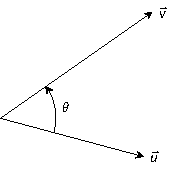
\includegraphics{figures/figdotpangle}\\
(a)\\[15pt]
\myincludegraphicsthree{width=125pt,3Dmenu,activate=onclick,deactivate=onclick,
3Droll=0,
3Dortho=0.0045,
3Dc2c=.54 .61 .58,
3Dcoo=0 0 40,
3Droo=170,
3Dlights=Headlamp,add3Djscript=asylabels.js}{}{figures/figdotpangle3D}\\
%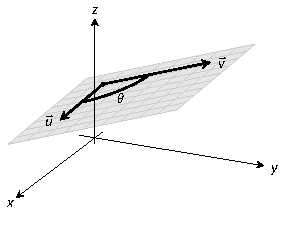
\includegraphics{figures/figdotpangle3D}\\
(b)
\end{tabular}
}

The same is also true of 2 vectors in space: given $\vec u$ and $\vec v$ in $\mathbb{R}^3$ with the same initial point, there is a plane that contains both $\vec u$ and $\vec v$. (When $\vec u$ and $\vec v$ are co-linear, there are infinite planes that contain both vectors.) In that plane, we can again find an angle $\theta$ between them (and again, $0\leq \theta\leq \pi$). This is illustrated in Figure \ref{fig:dotpangle}(b).

The following theorem connects this angle $\theta$ to the dot product of $\vec u$ and $\vec v$.

\theorem{thm:dot_product}{The Dot Product and Angles}
{Let $\vec u$ and $\vec v$ be vectors in $\mathbb{R}^2$ or $\mathbb{R}^3$. Then 
\[
\dotp uv = \norm{\vec u}\,\norm{\vec v} \cos\theta,
\]
where $\theta$, $0\leq\theta\leq \pi$, is the angle between $\vec u$ and $\vec v$.
\index{dot product!properties}\index{vectors!dot product}
}

\mfigure{.16}{Proving Theorem \ref{thm:dot_product}}{fig:dotprodproof}{figures/dotproductproof}

The proof of Theorem \ref{thm:dot_product} is an application of the \href{https://en.wikipedia.org/wiki/Law_of_cosines}{\underline{Law of Cosines}}, using the properties in Theorem \ref{thm:dot_product_properties}. Referring to Figure \ref{fig:dotprodproof}, if we let $a=\len{\vec u}$, $b=\len{\vec v}$, and $c = \len{\vec u-\vec v}$, then the Law of Cosines tells us that
\[
c^2 = a^2+b^2 - 2ab\cos(\theta).
\]
Thus, we have
\begin{align*}
\len{\vec{u}-\vec{v}}^2 & = \len{\vec{u}}^2+\len{\vec{v}}^2-2\len{\vec{u}}\len{\vec{v}}\cos\theta\\
(\vec u-\vec v)\boldsymbol{\cdot}(\vec u-\vec v) & = \dotp uu +\dotp vv -2\len{\vec{u}}\len{\vec{v}}\cos\theta\\
\dotp uu -\dotp uv - \dotp vu + \dotp vv & = \dotp uu +\dotp vv -2\len{\vec{u}}\len{\vec{v}}\cos\theta\\
-2\dotp uv &= -2\len{\vec{u}}\len{\vec{v}}\cos\theta\\
\dotp uv &= \len{\vec{u}}\len{\vec{v}}\cos\theta,
\end{align*}
as required.

When $\theta$ is an acute angle (i.e., $0\leq \theta <\pi/2$), $\cos \theta$ is positive; when $\theta = \pi/2$, $\cos \theta = 0$; when $\theta$ is an obtuse angle ($\pi/2<\theta \leq \pi$), $\cos \theta$ is negative. Thus the sign of the dot product gives a general indication of the angle between the vectors, illustrated in Figure \ref{fig:dotpsign}.

\begin{center}
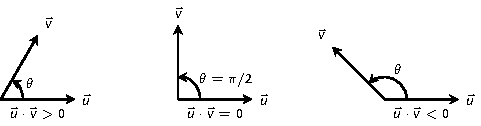
\includegraphics{figures/figdotpanglesign}
\captionsetup{type=figure}
\caption{Illustrating the relationship between the angle between vectors and the sign of their dot product.}
\label{fig:dotpsign}
\end{center}
\vskip\baselineskip

We \emph{can} use Theorem \ref{thm:dot_product} to compute the dot product, but generally this theorem is used to find the angle between known vectors (since the dot product is generally easy to compute). To this end, we rewrite the theorem's equation as
\[
\cos \theta = \frac{\dotp uv}{\norm{\vec u}\norm{\vec v}} \quad \Leftrightarrow \quad \theta = \cos^{-1}\left(\frac{\dotp uv}{\norm{\vec u}\norm{\vec v}}\right).
\]

We practice using this theorem in the following example.\\

\mfigure{.4}{Vectors used in Example \ref{ex_dotp2}.}{fig:dotp2}{figures/figdotp2}
\example{ex_dotp2}{Using the dot product to find angles}{
Let $\vec u = \la 3,1\ra$, $\vec v = \la -2,6\ra$ and $\vec w = \la -4,3\ra$, as shown in Figure \ref{fig:dotp2}. Find the angles $\alpha$, $\beta$ and $\theta$.
}
{We start by computing the magnitude of each vector.
\[
\norm{\vec u} = \sqrt{10};\quad \norm{\vec v} = 2\sqrt{10};\quad \norm{\vec w} = 5.
\]
We now apply Theorem \ref{thm:dot_product} to find the angles.
\begin{align*}
\alpha &= \cos^{-1}\left(\frac{\dotp uv}{(\sqrt{10})(2\sqrt{10})}\right) \\
			&= \cos^{-1}(0) = \frac{\pi}2 = 90^\circ.
\end{align*}
\begin{align*}
\beta &= \cos^{-1}\left(\frac{\dotp vw}{(2\sqrt{10})(5)}\right) \\
			&= \cos^{-1}\left(\frac{26}{10\sqrt{10}}\right) \\
					&\approx 0.6055 \approx 34.7^\circ.\\[10pt]
\theta &= \cos^{-1}\left(\frac{\dotp uw}{(\sqrt{10})(5)}\right) \\
				&= \cos^{-1}\left(\frac{-9}{5\sqrt{10}}\right) \\
				&\approx 2.1763 \approx 124.7^\circ
\end{align*}
\vskip-\baselineskip
}\\

We see from our computation that $\alpha + \beta = \theta$, as indicated by Figure \ref{fig:dotp2}. While we knew this should be the case, it is nice to see that this non-intuitive formula indeed returns the results we expected.

We do a similar example next in the context of vectors in space.\\

\example{ex_dotp3}{Using the dot product to find angles}{
Let $\vec u = \la 1,1,1\ra$, $\vec v = \la -1,3,-2\ra$ and $\vec w = \la -5,1,4\ra$, as illustrated in Figure \ref{fig:dotp3}. Find the angle between each pair of vectors.}
{\begin{enumerate}
	\item Between $\vec u$ and $\vec v$:
	\begin{align*}
	\theta &= \cos^{-1}\left(\frac{\dotp uv}{\norm{\vec u}\norm{\vec v}}\right)\\
					&= \cos^{-1}\left(\frac{0}{\sqrt{3}\sqrt{14}}\right)\\
					&= \frac{\pi}2.
	\end{align*}
	\item	Between $\vec u$ and $\vec w$:
	\begin{align*}
	\theta &= \cos^{-1}\left(\frac{\dotp uw}{\norm{\vec u}\norm{\vec w}}\right)\\
					&= \cos^{-1}\left(\frac{0}{\sqrt{3}\sqrt{42}}\right)\\
					&= \frac{\pi}2.
	\end{align*}
	\item	Between $\vec v$ and $\vec w$:
	\begin{align*}
	\theta &= \cos^{-1}\left(\frac{\dotp vw}{\norm{\vec v}\norm{\vec w}}\right)\\
					&= \cos^{-1}\left(\frac{0}{\sqrt{14}\sqrt{42}}\right)\\
					&= \frac{\pi}2.
	\end{align*}
\end{enumerate}
While our work shows that each angle is $\pi/2$, i.e.,  $90^\circ$, none of these angles looks to be a right angle in Figure \ref{fig:dotp3}. Such is the case when drawing three--dimensional objects on the page.
}\\

\mfigurethree{width=150pt,3Dmenu,activate=onclick,deactivate=onclick,
3Droll=0,
3Dortho=0.0045,
3Dc2c=.89 .4 .23,
3Dcoo=10 50 46,
3Droo=200,
3Dlights=Headlamp,add3Djscript=asylabels.js}{}{.7}{Vectors used in Example \ref{ex_dotp3}.}{fig:dotp3}{figures/figdotp3}%

All three angles between these vectors was $\pi/2$, or $90^\circ$. We know from geometry and everyday life that $90^\circ$ angles are ``nice'' for a variety of reasons, so it should seem significant that these angles are all $\pi/2$. Notice the common feature in each calculation (and also the calculation of $\alpha$ in Example \ref{ex_dotp2}): the dot products of each pair of angles was 0. We use this as a basis for a definition of the term \textbf{orthogonal}, which is essentially synonymous to \textit{perpendicular}.

\definition{def:orthogonal}{Orthogonal}
{Vectors $\vec u$ and $\vec v$ are \textbf{orthogonal} if their dot product is 0.
\index{orthogonal}\index{perpendicular|see{orthogonal}}\index{vectors!orthogonal}
}

\mnote{.22}{\textbf{Note:} The term \textit{perpendicular} originally referred to lines. As mathematics progressed, the concept of ``being at right angles to'' was applied to other objects, such as vectors and planes, and the term \emph{orthogonal} was introduced. It is especially used when discussing objects that are hard, or impossible, to visualize: two vectors in 5-dimensional space are orthogonal if their dot product is 0. It is not wrong to say they are \textit{perpendicular}, but common convention gives preference to the word \textit{orthogonal}.

Note also that Definition \ref{def:orthogonal} makes sense if either $\vec u$ or $\vec v$ is the zero vector, but this is not the case for the conventional understanding of the word perpendicular.
}

\pagebreak

\example{ex_dotp8}{Finding orthogonal vectors}{
Let $\vec u = \la 3,5\ra$ and $\vec v = \la 1,2,3\ra$. 
\begin{enumerate}
	\item Find two vectors in $\mathbb{R}^2$ that are orthogonal to $\vec u$.
	\item	Find two non--parallel vectors in $\mathbb{R}^3$ that are orthogonal to $\vec v$.
\end{enumerate}
}
{\begin{enumerate}
	\item Recall that a line perpendicular to a line with slope $m$ has slope $-1/m$, the ``opposite reciprocal slope.'' We can think of the slope of $\vec u$ as $5/3$, its ``rise over run.'' A vector orthogonal to $\vec u$ will have slope $-3/5$. There are many such choices, though all parallel:
	\[
	\la -5,3\ra \quad \text{or} \quad\la 5,-3\ra \quad \text{or} \quad \la -10,6\ra\quad \text{or} \quad \la 15,-9\ra,\text{etc.}
	\]
	\item		There are infinite directions in space orthogonal to any given direction, so there are an infinite number of non--parallel vectors orthogonal to $\vec v$. Since there are so many, we have great leeway in finding some.
	
	One way is to arbitrarily pick values for the first two components, leaving the third unknown. For instance, let $\vec v_1 = \la 2,7,z\ra$. If $\vec v_1$ is to be orthogonal to $\vec v$, then $\vec v_1\cdot\vec v = 0$, so 
	\[
	2+14+3z=0 \quad \Rightarrow z = \frac{-16}{3}.
	\]
	So $\vec v_1 = \la 2, 7, -16/3\ra$ is orthogonal to $\vec v$. We can apply a similar technique by leaving the first or second component unknown.
	
	Another method of finding a vector orthogonal to $\vec v$ mirrors what we did in part 1. Let $\vec v_2 = \la-2,1,0\ra$. Here we switched the first two components of $\vec v$, changing the sign of one of them (similar to the ``opposite reciprocal'' concept before). Letting the third component be 0 effectively ignores the third component of $\vec v$, and it is easy to see that 
	\[
	\vec v_2\cdot\vec v = \la -2,1,0\ra\cdot\la 1,2,3\ra = 0.
	\]
	Clearly $\vec v_1$ and $\vec v_2$ are not parallel.
\end{enumerate}
\vskip-1.5\baselineskip
}\\

An important construction is illustrated in Figure \ref{fig:dotpproj}, where vectors $\vec u$ and $\vec v$ are sketched. In part (a), a dotted line is drawn from the tip of $\vec u$ to the line containing $\vec v$, where the dotted line is orthogonal to $\vec v$. In part (b), the dotted line is replaced with the vector $\vec z$ and  $\vec w$ is formed, parallel to $\vec v$. It is clear by the diagram that $\vec u = \vec w+\vec z$. What is important about this construction is this: $\vec u$ is \emph{decomposed} as the sum of two vectors, one of which is parallel to $\vec v$ and one that is perpendicular to $\vec v$. It is hard to overstate the importance of this construction (as we'll see in upcoming examples). 

The vectors $\vec w$, $\vec z$ and $\vec u$ as shown in Figure \ref{fig:dotpproj} (b) form a right triangle, where the angle between $\vec v$ and $\vec u$ is labeled $\theta$. We can find $\vec w$ in terms of $\vec v$ and $\vec u$.

Using trigonometry, we can state that 
\begin{equation}
\norm{\vec w} = \norm{\vec u}\cos \theta. \label{eq:proj1}
\end{equation}
\mtable{.24}{Developing the construction of the \emph{orthogonal projection}.}{fig:dotpproj}{%
\begin{tabular}{c}
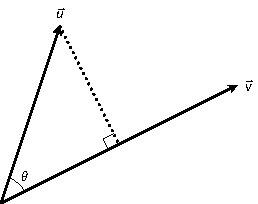
\includegraphics{figures/figdotpproja}\\
(a)\\[15pt]
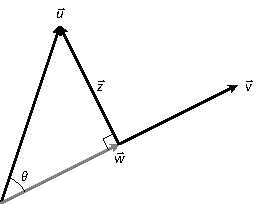
\includegraphics{figures/figdotpprojb}\\
(b)
\end{tabular}
}

We also know that $\vec w$ is parallel to to $\vec v$\,; that is, the direction of $\vec w$ is the direction of $\vec v$, described by the unit vector $\frac{1}{\norm{\vec v}}\vec v$. The vector $\vec w$ is the vector in the direction $\frac{1}{\norm{\vec v}}\vec v$ with magnitude $\norm{\vec u}\cos \theta$:

\begin{align*}
\vec w &= \Big(\norm{\vec u}\cos\theta \Big)\frac{1}{\norm{\vec v}}\vec v.\\
&= \left(\norm{\vec u}\frac{\dotp uv}{\norm{\vec u}\norm{\vec v}}\right)\frac{1}{\norm{\vec v}} \vec v \tag*{Replace $\cos\theta$ using Theorem \ref{thm:dot_product}}\\ 
			&= \frac{\dotp uv}{\norm{\vec v}^2}\vec v = \frac{\dotp uv}{\dotp vv}\vec v \tag*{Using Theorem \ref{thm:dot_product_properties}.}
\end{align*}

Since this construction is so important, it is given a special name.

\definition{def:orthogonal_projection}{Orthogonal Projection}
{Let $\vec u$ and $\vec v$ be given. The \textbf{orthogonal projection of $\vec u$ onto $\vec v$}, denoted $\proj uv$, is 
\index{orthogonal projection}\index{vectors!orthogonal projection}
\[
\proj uv = \left(\frac{\dotp uv}{\dotp vv}\right)\vec v.
\]
}\\

\enlargethispage{2\baselineskip}

\example{ex_dotp4}{Computing the orthogonal projection}{
\begin{enumerate}
	\item Let $\vec u= \la -2,1\ra$ and $\vec v=\la 3,1\ra$. Find $\proj uv$, and sketch all three vectors with initial points at the origin.
	\item	Let $\vec w = \la 2,1,3\ra$ and $\vec x = \la 1,1,1\ra$. Find $\proj wx$, and sketch all three vectors with initial points at the origin.
\end{enumerate}
}
{\begin{enumerate}
	\item Applying Definition \ref{def:orthogonal_projection}, we have
	\begin{align*}
	\proj uv &= \left(\frac{\dotp uv}{\dotp vv}\right)\vec v \\
					&= \frac{-5}{10}\la 3,1\ra\\
					&= \la -\frac32,-\frac12\ra.
	\end{align*}
	Vectors $\vec u$, $\vec v$ and $\proj uv$ are sketched in Figure \ref{fig:dotp4}(a). Note how the projection is parallel to $\vec v$; that is, it lies on the same line through the origin as $\vec v$, although it points in the opposite direction. That is because the angle between $\vec u$ and $\vec v$ is obtuse (i.e., greater than $90^\circ$).
\mtable{.37}{Graphing the vectors used in Example \ref{ex_dotp4}.}{fig:dotp4}{%
\begin{tabular}{c}
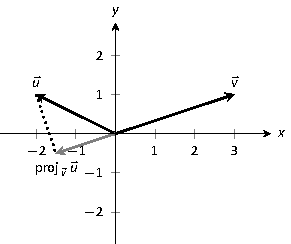
\includegraphics{figures/figdotp4a}\\
(a)\\[15pt]
\myincludegraphicsthree{width=100pt,3Dmenu,activate=onclick,deactivate=onclick,
3Droll=0,
3Dortho=0.0046,
3Dc2c=.9 .12 .42,
3Dcoo=0 50 30,
3Droo=250,
3Dlights=Headlamp,add3Djscript=asylabels.js}{}{figures/figdotp4b}\\
%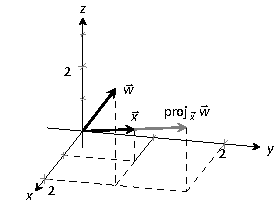
\includegraphics{figures/figdotp4b}\\
(b)\\[15pt]
\myincludegraphicsthree{width=100pt,3Dmenu,activate=onclick,deactivate=onclick,
3Droll=0,
3Dortho=0.0046,
3Dc2c=.29 .77 .56,
3Dcoo=50 0 40,
3Droo=250,
3Dlights=Headlamp,add3Djscript=asylabels.js}{}{figures/figdotp4c}\\
%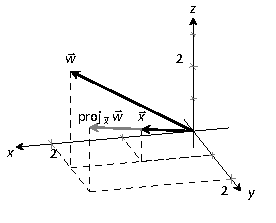
\includegraphics{figures/figdotp4c}\\
(c)\\[15pt]
\end{tabular}
}	
	
	\item		Apply the definition:
	\begin{align*}
	\proj wx &= \frac{\dotp wx}{\dotp xx}\vec x \\
					&= \frac{6}{3}\la 1,1,1\ra\\
					&= \la 2,2,2\ra.
	\end{align*}
	These vectors are sketched in Figure \ref{fig:dotp4}(b), and again in part (c) from a different perspective. Because of the nature of graphing these vectors, the sketch in part (b) makes it difficult  to recognize that the drawn projection has the geometric properties it should. The graph shown in part (c) illustrates these properties better.
\end{enumerate}
\vskip-\baselineskip
}

\pagebreak

Consider Figure \ref{fig:dotpprojc} where the concept of the orthogonal projection is again illustrated. It is clear that 
\begin{equation}
\vec u = \proj uv + \vec z.
\label{eq:orthogproj}
\end{equation} As we know what $\vec u$ and $\proj uv$ are, we can solve for $\vec z$ and state that
\[
\vec z = \vec u - \proj uv.
\]
This leads us to rewrite Equation \eqref{eq:orthogproj} in a seemingly silly way: 
\[
\vec u = \proj uv + (\vec u - \proj uv).
\]
This is not nonsense, as pointed out in the following Key Idea. (Notation note: the expression ``$\parallel \vec y$\,'' means ``is parallel to $\vec y$.'' We can use this notation to state ``$\vec x\parallel\vec y$\,'' which means ``$\vec x$ is parallel to $\vec y$.'' The expression ``$\perp \vec y$\,'' means ``is orthogonal to $\vec y$,'' and is used similarly.)

\mfigure{.73}{Illustrating the orthogonal projection.}{fig:dotpprojc}{figures/figdotpprojc}

\mnote{.4}{\textbf{Note:} The argument leading to Definition \ref{def:orthogonal_projection} is not quite a proof, since it depended on choices made in forming the diagram in Figure \ref{fig:dotpproj}. However, we can easily verify that the result in Key Idea \ref{idea:orthog_proj} is always valid: since
\begin{align*}
\vec v\boldsymbol{\cdot}(\vec u - \proj uv) & = \dotp vu - \vec v\boldsymbol{\cdot}\left(\frac{\dotp uv}{\len{\vec{v}}^2}\vec{v}\right)\\
& = \dotp vu -\frac{\dotp uv}{\dotp vv}(\dotp vv)\\
& = \dotp vu - \dotp uv = 0
\end{align*}
for \textbf{any} vectors $\vec u$ and $\vec v\neq \vec 0$, we are guaranteed that the vector $u-\proj uv$ will always be orthogonal to $\vec v$.}

\keyidea{idea:orthog_proj}{Orthogonal Decomposition of Vectors}
{Let $\vec u$ and $\vec v$ be given. Then $\vec u$ can be written as the sum of two vectors, one of which is parallel to $\vec v$, and one of which is orthogonal to $\vec v$:
\index{orthogonal decomposition of vectors}\index{orthogonal!decomposition}\index{vectors!orthogonal decomposition}
\[
\vec u = \underbrace{\proj uv}_{\parallel\ \vec v}\ +\  (\underbrace{\vec u-\proj uv}_{\perp\ \vec v}).
\]
}

We illustrate the use of this equality in the following example.\\

\example{ex_dotp5}{Orthogonal decomposition of vectors}{
\begin{enumerate}
	\item Let $\vec u = \la -2,1\ra $ and $\vec v = \la 3,1\ra$ as in Example \ref{ex_dotp4}. Decompose $\vec u$ as the sum of a vector parallel to $\vec v$ and a vector orthogonal to $\vec v$.
	\item	Let $\vec w =\la 2,1,3\ra$ and $\vec x  =\la 1,1,1\ra$ as in Example \ref{ex_dotp4}. Decompose $\vec w$ as the sum of a vector parallel to $\vec x$ and a vector orthogonal to $\vec x$.
\end{enumerate}
}
{\begin{enumerate}
	\item In Example \ref{ex_dotp4}, we found that $\proj uv = \la -1.5,-0.5\ra$. Let 
	\[
	\vec z = \vec u - \proj uv = \la -2,1\ra - \la -1.5,-0.5\ra = \la-0.5, 1.5\ra.
	\]
	Is $\vec z$ orthogonal to $\vec v$\,? (I.e, is $\vec z \perp\vec v$\ ?) We check for orthogonality with the dot product:
	\[
	\dotp zv = \la -0.5,1.5\ra \cdot \la 3,1\ra =0.
	\]
	Since the dot product is 0, we know $\vec z \perp \vec v$. Thus:
	\begin{align*}
	\vec u &= \proj uv\ +\ (\vec u - \proj uv) \\
	\la -2,1\ra &= \underbrace{\la -1.5,-0.5\ra}_{\parallel\ \vec v}\ +\ \underbrace{\la -0.5,1.5\ra}_{\perp \ \vec v}.
	\end{align*}
	
	\item	We found in Example \ref{ex_dotp4} that $\proj wx = \la 2,2,2\ra$. Applying the Key Idea, we have:
	\[
	\vec z = \vec w - \proj wx = \la 2,1,3\ra  - \la 2,2,2\ra = \la 0,-1,1\ra.
	\]
	We check to see if $\vec z \perp \vec x$:
\[
\dotp zx = \la 0,-1,1\ra \cdot \la 1,1,1\ra = 0.
\]
	Since the dot product is 0, we know the two vectors are orthogonal.
	We now write $\vec w$ as the sum of two vectors, one parallel and one orthogonal to $\vec x$:
	\begin{align*}
	\vec w &= \proj wx\ +\ (\vec w - \proj wx) \\
	\la 2,1,3\ra &= \underbrace{\la 2,2,2\ra}_{\parallel\ \vec x}\ +\ \underbrace{\la 0,-1,1\ra}_{\perp \ \vec x} 
	\end{align*}
\end{enumerate}
\vskip-\baselineskip
}\\

We give an example of where this decomposition is useful.\\

\example{ex_dotp6}{Orthogonally decomposing a force vector}{
Consider Figure \ref{fig:dotp6}(a), showing a box weighing 50lb on a ramp that rises 5ft over a span of 20ft. Find the components of force, and their magnitudes, acting on the box (as sketched in part (b) of the figure):
\mtable{.4}{Sketching the ramp and box in Example \ref{ex_dotp6}. Note: \textit{The vectors are not drawn to scale.}}{fig:dotp6}{%
\begin{tabular}{c}
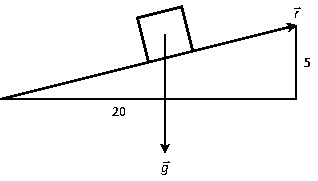
\includegraphics{figures/figdotp6}\\
(a)\\[15pt]
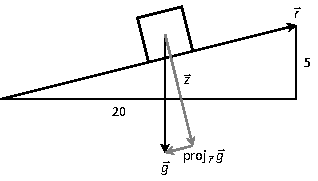
\includegraphics{figures/figdotp6b}\\
(b)
\end{tabular}
}
\begin{enumerate}
	\item in the direction of the ramp, and
	\item	orthogonal to the ramp.
\end{enumerate}
}
{As the ramp rises 5ft over a horizontal distance of 20ft, we can represent the direction of the ramp with the vector $\vec r= \la 20,5\ra$. Gravity pulls down with a force of 50lb, which we represent with $\vec g = \la 0,-50\ra$. 
\begin{enumerate}
	\item To find the force of gravity in the direction of the ramp, we compute $\proj gr$:
	\begin{align*}
	\proj gr &= \frac{\dotp gr}{\dotp rr}\vec r\\
					&=  \frac{-250}{425}\la 20,5\ra\\
					&= \la -\frac{200}{17},-\frac{50}{17}\ra \approx \la -11.76,-2.94\ra.
	\end{align*}
	The magnitude of $\proj gr$ is $\norm{\proj gr} = 50/\sqrt{17} \approx 12.13\text{lb}$. Though the box weighs 50lb, a force of about 12lb is enough to keep the box from sliding down the ramp.

\enlargethispage{2\baselineskip}
	
	\item		To find the component $\vec z$ of gravity orthogonal to the ramp, we use Key Idea \ref{idea:orthog_proj}.
	\begin{align*}
	\vec z &= \vec g - \proj gr \\
					&= \la \frac{200}{17},-\frac{800}{17}\ra \approx \la 11.76,-47.06\ra.
	\end{align*}
	The magnitude of this force is $\norm{\vec z} \approx 48.51$lb. In physics and engineering, knowing this force is important when computing things like static frictional force. (For instance, we could easily compute if the static frictional force alone was enough to keep the box from sliding down the ramp.)
\end{enumerate}
\vskip-\baselineskip
}

\pagebreak

\noindent\textbf{\large Application to Work}\\

In physics, the application of a force $F$ to move an object in a straight line a distance $d$ produces \emph{work}; the amount of work $W$ is $W=Fd$, (where $F$ is in the direction of travel). The orthogonal projection allows us to compute work when the force is not in the direction of travel.

Consider Figure \ref{fig:dotpwork}, where a force $\vec F$ is being applied to an object moving in the direction of $\vec d$. (The distance the object travels is the magnitude of $\vec d$.) The work done is the amount of force in the direction of $\vec d$, $\norm{\proj Fd}$, times $\vnorm d$:
\mfigure{.75}{Finding work when the force and direction of travel are given as vectors.}{fig:dotpwork}{figures/figdotpwork}

\begin{align*}
\norm{\proj Fd}\cdot\vnorm d &= \snorm{\frac{\dotp Fd}{\dotp dd}\vec d}\cdot \vnorm d \\
		&= \left|\frac{\dotp Fd}{\vnorm d^2}\right|\cdot \vnorm d\cdot\vnorm d\\
		&= \frac{\left|\dotp Fd\right|}{\vnorm d^2}\vnorm d^2\\
		&= \left|\dotp Fd\right|.
\end{align*}

The expression $\dotp Fd$ will be positive if the angle between $\vec F$ and $\vec d$ is acute; when the angle is obtuse (hence $\dotp Fd$ is negative), the force is causing motion in the opposite direction of $\vec d$, resulting in ``negative work.'' We want to capture this sign, so we drop the absolute value and find that $W = \dotp Fd$.

\definition{def:work}{Work}
{Let $\vec F$ be a constant force that moves an object in a straight line from point $P$ to point $Q$. Let $\vec d = \vv{PQ}$. The \textbf{work} $W$ done by $\vec F$ along $\vec d$ is $W = \dotp Fd$.
\index{work}
}

\example{ex_dotp7}{Computing work}{
A man slides a box along a ramp that rises 3ft over a distance of 15ft by applying 50lb of force as shown in Figure \ref{fig:dotp7}. Compute the work done.}
{The figure indicates that the force applied makes a $30^\circ$ angle with the horizontal, so $\vec F = 50\la \cos 30^\circ,\sin 30^\circ\ra \approx \la 43.3,25\ra.$ The ramp is represented by $\vec d  = \la 15,3\ra$. The work done is simply
\[
\dotp Fd = 50\la \cos 30^\circ,\sin 30^\circ\ra \cdot \la 15,3\ra \approx 724.5 \text{ft--lb}.
\]

\mfigure{.4}{Computing work when sliding a box up a ramp in Example \ref{ex_dotp7}.}{fig:dotp7}{figures/figdotp7}
Note how we did not actually compute the distance the object traveled, nor the magnitude of the force in the direction of travel; this is all inherently computed by the dot product!
}\\

The dot product is a powerful way of evaluating computations that depend on angles without actually using angles. The next section explores another ``product'' on vectors, the \emph{cross product.} Once again, angles play an important role, though in a much different way.

\printexercises{exercises/10_03_exercises}

\section{The Cross Product}\label{sec:cross_product}

``Orthogonality'' is immensely important. A quick scan of your current environment will undoubtedly reveal numerous surfaces and edges that are perpendicular to each other (including the edges of this page). The dot product provides a quick test for orthogonality:  vectors $\vec u$ and $\vec v$ are perpendicular if, and only if, $\dotp uv=0$. 

Given two non--parallel, nonzero vectors $\vec u$ and $\vec v$ in space, it is very useful to find a vector $\vec w$ that is perpendicular to both $\vec u$ and $\vec v$. There is a operation, called the \textbf{cross product}, that creates such a vector. This section defines the cross product, then explores its properties and applications.

\definition{def:cross_product}{Cross Product}
{Let $\vec u =\la u_1,u_2,u_3\ra$ and $\vec v = \la v_1,v_2,v_3\ra$ be vectors in $\mathbb{R}^3$. The \textbf{cross product of $\vec u$ and $\vec v$}, denoted $\crossp uv$, is the vector
\index{vectors!cross product}\index{cross product!definition}
\[
\crossp uv = \la u_2v_3-u_3v_2,u_3v_1-u_1v_3,u_1v_2-u_2v_1\ra.
\]
}

\mnote{.6}{The definition of the cross product may look strange (and complicated) at first, but it's more or less forced by the requirement that it be orthogonal to both $\vec u$ and $\vec v$. To begin to see why, suppose $\vec w = \la a,b,c\ra$ is an arbitrary vector such that $\dotp wu=0$ and $\dotp wv=0$. This gives us the pair of equations
\begin{align*}
u_1a+u_2b+u_3c&=0\\
v_1a+v_2b+v_3c&=0.
\end{align*}
This is a \textit{system of linear equations} in the variables $a$, $b$, and $c$. We'll learn the techniques for solving any such system in Chapter \ref{chapter:linear}, at which point we'll be able to see that (up to a scalar multiple) the solution is given by Definition \ref{def:cross_product}.}

This definition can be a bit cumbersome to remember. After an example we will give a convenient method for computing the cross product. For now, careful examination of the products and differences given in the definition should reveal a pattern that is not too difficult to remember. (For instance, in the first component only 2 and 3 appear as subscripts; in the second component, only 1 and 3 appear as subscripts. Further study reveals the order in which they appear.)

Let's practice using this definition by computing a cross product.\\

\example{ex_crossp1}{Computing a cross product}{
Let $\vec u = \la 2,-1,4\ra$ and $\vec v = \la 3,2,5\ra$. Find $\crossp uv$, and verify that it is orthogonal to both $\vec u$ and $\vec v$.
}
{Using Definition \ref{def:cross_product}, we have
\begin{align*}
\crossp uv &= \la u_2v_3-u_3v_2,u_3v_1-u_1v_3,u_1v_2-u_2v_1\ra\\
		   &= \la (-1)5-(4)2,(4)3-(2)5, (2)2-(-1)3\ra = \la -13,2,7\ra.
\end{align*}
(We encourage the reader to compute this product on their own, then verify their result.)

We test whether or not $\crossp uv$ is orthogonal to $\vec u$ and $\vec v$ using the dot product:
\begin{align*}
\big(\crossp uv\big) \cdot \vec u &= \la -13,2,7\ra \cdot \la 2,-1,4\ra = 0,\\
\big(\crossp uv\big) \cdot \vec v &= \la -13,2,7\ra \cdot \la 3,2,5 \ra = 0.
\end{align*}
Since both dot products are zero, $\crossp uv$ is indeed orthogonal to both $\vec u$ and $\vec v$.
}\\

We now introduce a method for computing the cross-product that is easier to remember, and has the added benefit of allowing us to preview \sword{determinants}, which we will return to in earnest in Section \ref{sec:determinant_1}. 

Consider a rectangular array $\bbm a&b\\c&d\ebm$ of four real numbers $a,b,c$, and $d$. A $2\times 2$ determinant takes any such array and assigns the number $ad-bc$. This is commonly denoted as follows:
\[
\bvm a&b\\c&d\evm = ad-bc.
\]
Most people find it easiest to remember this in terms of the two \textit{diagonals} of the array: we take the product of the two numbers on the \textit{main diagonal} (top-left to bottom-right), and subtract the product of the two numbers on the other diagonal:
\btz [baseline=-3pt,>=stealth]
\node at (0,0) {$\bvm a & b\\ c& d\evm$};
\draw[->,  thin] (-.5,.4) -- (.6,-.6) node[below right] {$ac\vphantom{bd}$};
\draw[->, thin] (0.4,.4) -- (-.6,-.6) node[below left ] {$bd$};
\etz

For example, we have $\bvm 4&-2\\6&3\evm = 4(3)-(-2)(6)=24$. Once we get comfortable with $2\times 2$ determinants, we can write the cross product in terms of them, as follows:
\begin{align}
\crossp uv &= \bvm u_2&u_3\\v_2&v_3\evm \veci - \bvm u_1&u_3\\v_1&v_3\evm\vecj + \bvm u_1&u_2\\v_1&v_2\evm\veck\label{eq:crossdet}\\ 
& = (u_2v_3-u_3v_2)\veci-(u_3v_1-u_1v_3)\vecj + (u_1v_2-u_2v_1)\veck,\nonumber
\end{align}
as before. Now, this might not seem like much of an improvement over the previous formula, so we take things one step further. First, we form a $3\times 3$ array as shown below. 
\[
\bvm \veci&\vecj&\veck\\u_1&u_2&u_3\\v_1&v_2&v_3\evm.
\]
The first row comprises the standard unit vectors $\vec i$, $\vec j$, and $\vec k$. The second and third rows are the vectors $\vec u$ and $\vec v$, respectively. Next, we \textit{expand} our $3\times 3$ array as a vector, where the coefficient of each standard unit vector is given by the $2\times 2$ determinant that's left over when we delete the row and column containing that unit vector. 

For example, if we use $\vec u$ and $\vec v$ from Example \ref{ex_crossp1}, we obtain the array
\[
\bvm \veci&\vecj&\veck \\  2&-1&4\\3&2&5\evm.
\]
The expansion process used to obtain the coefficients of $\veci, \vecj \veck$ looks like the following:

\btz [baseline=-3pt,>=stealth]
\node at (0,0) {$\bvm \fbox{\veci}&\vecj&\veck \\  2&-1&4\\3&2&5\evm\longrightarrow \bvm -1&4\\2&5\evm\veci = -13\veci$};
\draw[thin] (-2.3,.6) -- (-2.3, -.6);
\draw[thin] (-2.5,.4) -- (-.8,.4);
\etz

\btz [baseline=-3pt,>=stealth]
\node at (0,0) {$\bvm \veci&\fbox{\vecj}&\veck \\  2&-1&4\\3&2&5\evm\longrightarrow \bvm 2&4\\3&5\evm\vecj = -2\vecj$};
\draw[thin] (-1.45,.6) -- (-1.45, -.6);
\draw[thin] (-2.3,.4) -- (-.6,.4);
\etz

\btz [baseline=-3pt,>=stealth]
\node at (0,0) {$\bvm \veci&\vecj&\fbox{\veck} \\  2&-1&4\\3&2&5\evm\longrightarrow \bvm 2&-1\\3&2\evm\veck = 7\veck$};
\draw[thin] (-0.85,.6) -- (-0.85, -.6);
\draw[thin] (-2.3,.4) -- (-.6,.4);
\etz

There is one more important detail to note: notice in Equation \eqref{eq:crossdet} that there is a \textbf{minus sign} in front of the coefficient of the unit vector $\vecj$. We need to make sure that the signs in front of each $2\times 2$ determinant follow this $+,\,-,\,+$ pattern when we expand our array as a vector. For the vectors $\vec u$ and $\vec v$ in Example \ref{ex_crossp1}, we end up with the following:
\begin{align*}
\crossp uv & = \bvm \veci&\vecj&\veck \\  2&-1&4\\3&2&5\evm  = \bvm -1&4\\2&5\evm\veci - \bvm 2&4\\3&5\evm\vecj + \bvm 2&-1\\3&2\evm\veck\\
& = -13\veci - (-2)\vecj + 7\veck = \la -13, 2, 7\ra,
\end{align*}
as before. The method will become more clear with a bit of practice.\\

\mnote{.75}{\textbf{Note:} If the minus sign in front of the $\vecj$ coefficient seems out of place to you, it might help to imagine wrapping our $3\times 3$ array around a cylinder (like the label on a tin can). If we read from left to right, \textit{beginning in the $\vecj$ column}, then we should place the $\veck$ column first, followed by the $\veci$ column. For the vectors $\vec{u}$ and $\vec{v}$ in Example \ref{ex_crossp1}, this would result in the coefficient $\bvm 4&2\\5&2\evm = 2$ for the $\vecj$ component, which has the correct sign. However, since our habit is to read starting from the far left, we tend to write the $\veci$ column first, and then introduce the minus sign to compensate.}


\example{ex_crossp2}{Computing a cross product}{
Let $\vecu=\la 1,3,6\ra$ and $\vec v = \la -1,2,1\ra$. Compute both $\crossp uv$ and $\crossp vu$.}
{To compute $\crossp uv$, we form our $3\times 3$ array as prescribed above, and expand it into a vector:
\begin{align*}
\crossp uv &= \bvm \veci & \vecj & \veck\\ 1& 3& 6\\ -1& 2& 1\evm = \bvm 3& 6\\2 &1\evm \veci - \bvm 1 & 6\\ -1& 1\evm\vecj +\bvm 1& 3\\ -1 & 2\evm\veck\\
		& = (3(1)-6(2))\veci -(1(1)-6(-1))\vecj + (1(2)-3(-1))\veck\\
		& = -9\veci-7\vecj+5\veck = \la -9, -7, 5\ra.
\end{align*}
To compute $\crossp vu$, we switch the second and third rows of the above matrix, then expand as before:
\begin{align*}
\crossp vu & = \bvm \veci & \vecj& \veck\\ -1 & 2& 1\\ 1& 3& 6\evm = \bvm 2 &1\\3 &6\evm\veci - \bvm -1& 1\\ 1& 6\evm\vecj + \bvm -1& 2\\ 1 &3\evm\veck\\
		   & = (2(6)-1(3))\veci-((-1)(6)-1(1))\vecj + ((-1)(3)-2(1))\veck\\
		   & = 9\veci+7\vecj -5\veck = \la 9, 7, -5\ra = -\crossp uv.
\end{align*}
Note how with the rows being switched, the products that once appeared on the right now appear on the left, and vice--versa, so that the result is the opposite of $\crossp uv$. We leave it to the reader to verify that each of these vectors is orthogonal to $\vec u$ and $\vec v$.
}\\

\noindent\textbf{\large Properties of the Cross Product}\\

It is not coincidence that $\crossp vu = -(\crossp uv)$ in the preceding example; one can show using Definition \ref{def:cross_product} that this will always be the case. The following theorem states several useful properties of the cross product, each of which can be verified by referring to the definition.

\setboxwidth{15pt}
%\noindent\hskip-50pt\begin{minipage}{\linewidth}
\theorem{thm:cross_prod_prop}{Properties of the Cross Product}
{Let $\vecu$, $\vecv$ and $\vecw$ be vectors in $\mathbb{R}^3$ and let $c$ be a scalar. The following identities hold:
\index{vectors!cross product}\index{cross product!properties}
\begin{enumerate}
	\item \parbox{167pt}{$\crossp uv = -(\crossp vu)$} Anticommutative Property
	\item	\begin{enumerate}
		\item \parbox{145pt}{$(\vec u+\vec v)\times \vecw = \crossp uw+\crossp vw$} Distributive Properties
		\item	$\vec u \times (\vec v+\vec w) = \crossp uv+\crossp uw$
	\end{enumerate}
	\item		$c(\crossp uv) = (c\vecu) \times \vec v = \vecu \times (c\vecv)$
	\item		\begin{enumerate}
		\item \parbox{145pt}{$(\crossp uv)\cdot \vecu = 0$} Orthogonality Properties
		\item	$(\crossp uv)\cdot \vecv = 0$
	\end{enumerate}
	\item		$\crossp uu = \vec 0$
	\item		$\crossp u0 = \vec 0$
	\item		\parbox{167pt}{$\vecu \boldsymbol{\cdot} (\vecv\times\vecw) = (\crossp uv)\boldsymbol{\cdot} \vecw$} Scalar Triple Product
\end{enumerate}
}
%\end{minipage}
\restoreboxwidth

We introduced the cross product as a way to find a vector orthogonal to two given vectors, but we did not give a proof that the construction given in Definition \ref{def:cross_product} satisfies this property. Theorem \ref{thm:cross_prod_prop} asserts this property holds; we leave it as a problem in the Exercise section to verify this.

The algebraic properties of the cross product in Theorem \ref{thm:cross_prod_prop} also give us an additional method for computing the cross product in terms of the unit vectors $\veci, \vecj, \veck$. We know from Property 5 that
\[
\veci\times\veci = \vec 0, \vecj\times\vecj = \vec 0, \veck\times\veck = \vec 0,
\]
and it's easy to check that
\[
\veci\times\vecj = \veck, \vecj\times\veck = \veci, \veck\times\veci=\vecj,
\]
and then Property 1 guarantees that
\[
\vecj\times \veci = -\veck, \veck\times\vecj = -\veci, \veci\times\veck = -\vecj.
\]
Using Properties 2 and 3, we can then compute, for example,
\begin{align*}
\la 2,0,3\ra\times \la -1,4,2\ra & = (2\veci +3\veck)\times (-\veci +4\vecj +2\veck)\\
& = -2(\veci \times \veci)+8(\veci \times\vecj)+4(\veci \times\veck)\\
& \quad \quad-3(\veck\times\veci)+12(\veck\times\vecj)+6(\veck\times\veck)\\
& = \vec 0+8\veck -4\vecj -3\vecj -12\veci + \vec 0 = \la -12, -7, 8\ra.
\end{align*}

Property 5 from the theorem is also left to the reader to prove in the Exercise section, but it reveals something more interesting than ``the cross product of a vector with itself is $\vec 0$.'' Let $\vec u$ and $\vec v$ be parallel vectors; that is, let there be a scalar $c$ such that $\vecv = c\vecu$. Consider their cross product:
\begin{align*}
\crossp uv &= \vecu \times (c\vec u) \\
					&=	\parbox{50pt}{$c(\crossp uu)$}\text{(by Property 3 of Theorem \ref{thm:cross_prod_prop})}\\
					&= \parbox{50pt}{$\vec 0$.}\text{(by Property 5 of Theorem \ref{thm:cross_prod_prop})}
\end{align*}

We have just shown that the cross product of parallel vectors is $\vec 0$. This hints at something deeper. Theorem \ref{thm:dot_product} related the angle between two vectors and their dot product; there is a similar relationship relating the cross product of two vectors and the angle between them, given by the following theorem.

\theorem{thm:cross_product}{The Cross Product and Angles}
{Let $\vec u$ and $\vec v$ be vectors in $\mathbb{R}^3$. Then
\[
\norm{\crossp uv} = \vnorm u\, \vnorm v \sin\theta,
\]
where $\theta$, $0\leq \theta \leq \pi$, is the angle between $\vecu$ and $\vecv$.
\index{vectors!cross product}\index{cross product!properties}
}

\mnote{.52}{\textbf{Note:} Definition \ref{def:orthogonal} (through Theorem \ref{thm:dot_product}) defines $\vec u$ and $\vec v$ to be orthogonal if $\vec u\cdot\vec v=0$. We could use Theorem \ref{thm:cross_product} to define $\vec u$ and $\vec v$ are parallel if $\vec u\times \vec v = 0$. By such a definition, $\vec 0$ would be both orthogonal and parallel to every vector. Apparent paradoxes such as this are not uncommon in mathematics and can be very useful. (See also the first marginal note on page \pageref{note:parallel}.)\label{note:crossp}}
Note that this theorem makes a statement about the \emph{magnitude} of the cross product. When the angle between $\vecu$ and $\vecv$ is 0 or $\pi$ (i.e., the vectors are parallel), the magnitude of the cross product is 0. The only vector with a magnitude of 0 is $\vec 0$ (see Property \ref{thm:zero_norm} of Theorem \ref{thm:vector_properties}), hence the cross product of  parallel vectors is $\vec 0$.\\

We provide some anecdotal evidence of the truth of this theorem in the following example.\\

\example{ex_crossp3}{The cross product and angles}{
Let $\vec u = \la 1,3,6\ra$ and $\vec v = \la -1,2,1\ra$ as in Example \ref{ex_crossp2}. Verify Theorem \ref{thm:cross_product} by finding $\theta$, the angle between $\vecu$ and $\vecv$, and the magnitude of $\crossp uv$.}
{We use Theorem \ref{thm:dot_product} to find the angle between $\vecu$ and $\vecv$. 
\begin{align*}
\theta &= \cos^{-1}\left(\frac{\dotp uv}{\vnorm u\, \vnorm v}\right) \\
			&= \cos^{-1}\left(\frac{11}{\sqrt{46}\sqrt{6}}\right)\\
			&\approx 0.8471 = 48.54^\circ.
\end{align*}

Our work in Example \ref{ex_crossp2} showed that $\crossp uv = \la -9,-7,5\ra$, hence $\norm{\crossp uv} = \sqrt{155}.$ Is $\norm{\crossp uv} = \vnorm u\, \vnorm v\sin\theta$? Using numerical approximations, we find:
\begin{align*}
\norm{\crossp uv} &=\sqrt{155}  & \vnorm u\,\vnorm v \sin\theta & = \sqrt{46}\sqrt{6}\sin 0.8471\\
									&\approx 12.45. & &\approx 12.45.
\end{align*}
Numerically, they seem equal. Using a right triangle, one can show that 
\[
\sin\left(\cos^{-1}\left(\frac{11}{\sqrt{46}\sqrt{6}}\right)\right) = \frac{\sqrt{155}}{\sqrt{46}\sqrt{6}},
\]
which allows us to verify the theorem exactly.
}\\

To see that Theorem \ref{thm:cross_product} holds in general, let $\vec u=\la u_1,u_2,u_3\ra$ and $\vec v =\la v_1,v_2,v_3\ra$ be two arbitrary vectors in $\R^3$. Since the angle between $\vec u$ and $\vec v$ is defined to lie between 0 and $\pi$, we know that $\sin\theta\geq 0$, so that both sides of the equation $\len{\crossp uv} = \len{\vec{u}}\len{\vec v}\sin\theta$ are positive. Thus, we can show that both sides are equal if we can show that their squares are equal. We have
\begin{align*}
(\len{\vec u}\len{\vec v}\sin\theta)^2 & = \len{\vec u}^2\len{\vec v}^2\sin^2\theta\\
& = \len{\vec u}^2\len{\vec v}^2(1-\cos^2\theta) \tag*{since $\sin^2\theta+\cos^2\theta=1$}\\
& = \len{\vec u}^2\len{\vec v}^2-(\len{\vec u}\len{\vec v}\cos\theta)^2\\
& = \len{\vec u}^2\len{\vec v}^2-(\dotp uv)^2 \tag*{by Theorem \ref{thm:dot_product}}\\
& = (u_1^2+u_2^2+u_3^2)(v_1^2+v_2^2+v_3^2)-(u_1v_1+u_2v_2+u_3v_3)^2\\
& = u_2^2v_3^2 - 2u_2u_3v_2v_3 + u_3^2v_2^2 + u_1v_3^2 - 2u_1u_3v_1v_3 \tag*{$+ u_3^2v_1^2 + u_1^2v_2^2 - 2u_1u_2v_1v_2 + u_2^2v_1^2$}\\
& = (u_2v_3-u_3v_2)^2+(u_3v_1-u_1v_3)^2+(u_1v_2-u_2v_2)^2\\
& = \len{\crossp uv}^2,
\end{align*}
as required.\\




\noindent\textbf{Right Hand Rule}\\

The anticommutative property of the cross product demonstrates that $\crossp uv$ and $\crossp vu$ differ only by a sign -- these vectors have the same magnitude but point in the opposite direction. When seeking a vector perpendicular to $\vec u$ and $\vec v$, we essentially have two directions to choose from, one in the direction of $\crossp uv$ and one in the direction of $\crossp vu$. Does it matter which we choose? How can we tell which one we will get without graphing, etc.?

Another wonderful property of the cross product, as defined, is that it follows the \textbf{right hand rule.} Given $\vec u$ and $\vec v$ in $\mathbb{R}^3$ with the same initial point, point the index finger of your right hand in the direction of $\vecu$ and let your middle finger point in the direction of $\vecv$ (much as we did when establishing the right hand rule for the 3-dimensional coordinate system). Your thumb will naturally extend in the direction of $\crossp uv$. One can ``practice'' this using Figure \ref{fig:crossp_rhr}. If you switch, and point the index finder in the direction of $\vecv$ and the middle finger in the direction of $\vecu$, your thumb will now point in the opposite direction, allowing you to ``visualize'' the anticommutative property of the cross product.
\mfigurethree{width=150pt,3Dmenu,activate=onclick,deactivate=onclick,
3Droll=0,
3Dortho=0.0044,
3Dc2c=.78 .32 .53,
3Dcoo=0 0 34,
3Droo=150,
3Dlights=Headlamp,add3Djscript=asylabels.js}{scale=1.25,trim=5mm 5mm 5mm 5mm,clip=true}{.5}{Illustrating the Right Hand Rule of the cross product.}{fig:crossp_rhr}{figures/figcrossp_rhr}
%\mfigure[scale=1.25,trim=5mm 5mm 5mm 5mm,clip=true]{.5}{Illustrating the Right Hand Rule of the cross product.}{fig:crossp_rhr}{figures/figcrossp_rhr}

\vskip\baselineskip
\noindent\textbf{\large Applications of the Cross Product}\\

There are a number of ways in which the cross product is useful in mathematics, physics and other areas of science beyond ``just'' finding a vector perpendicular to two others. We highlight a few here.\index{cross product!applications}\\
%\enlargethispage{\baselineskip}
%	\clearpage\enlargethispage{2\baselineskip}

\noindent\textbf{Area of a Parallelogram}\\

It is a standard geometry fact that the area of a parallelogram is $A = bh$, where $b$ is the length of the base and $h$ is the height of the parallelogram, as illustrated in Figure \ref{fig:crossp_parallelogram}(a). As shown when defining the Parallelogram Law of vector addition, two vectors $\vecu$ and $\vecv$ define a parallelogram when drawn from the same initial point, as illustrated in Figure \ref{fig:crossp_parallelogram}(b). Trigonometry tells us that $h = \vnorm u \sin \theta$, hence the area of the parallelogram is 
\begin{equation}A = \vnorm u\,\vnorm v\sin\theta = \norm{\crossp uv},\label{eq:crossp1}\end{equation}
where the second equality comes from Theorem \ref{thm:cross_product}.
\mtable{.23}{Using the cross product to find the area of a parallelogram.}{fig:crossp_parallelogram}{%
\begin{tabular}{c}
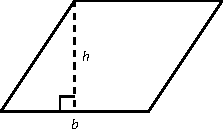
\includegraphics{figures/figcrossp_parallelogram1}\\
(a) \\[15pt]
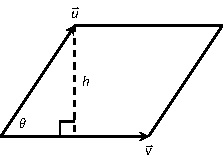
\includegraphics{figures/figcrossp_parallelogram2}\\
(b) \\
\end{tabular}
}
We illustrate using Equation \eqref{eq:crossp1} in the following example.
\index{cross product!applications!area of parallelogram}\\

\example{ex_crossp4}{Finding the area of a parallelogram}{
\begin{enumerate}
	\item Find the area of the parallelogram defined by the vectors $\vecu = \la 2,1\ra$ and $\vecv = \la 1,3\ra$.
	\item	Verify that the points $A = (1,1,1)$, $B = (2,3,2)$, $C = (4,5,3)$ and $D = (3,3,2)$ are the vertices of a parallelogram. Find the area of the parallelogram.
\end{enumerate}
}
{\begin{enumerate}
	\item Figure \ref{fig:crossp4}(a) sketches the parallelogram defined by the vectors $\vec u$ and $\vec v$. We have a slight problem in that our vectors exist in $\mathbb{R}^2$, not $\mathbb{R}^3$, and the cross product is only defined on vectors in $\mathbb{R}^3$. We skirt this issue by viewing $\vec u$ and $\vecv$ as vectors in the $x-y$ plane of $\mathbb{R}^3$, and rewrite them as $\vec u = \la 2,1,0\ra$ and $\vecv =\la 1,3,0\ra$. We can now compute the cross product. 
	It is easy to show that $\crossp uv = \la 0,0,5\ra$; therefore the area of the parallelogram is $A = \norm{\crossp uv} = 5$.
	\mtable{.65}{Sketching the parallelograms in Example \ref{ex_crossp4}.}{fig:crossp4}{%
	\begin{tabular}{c}
	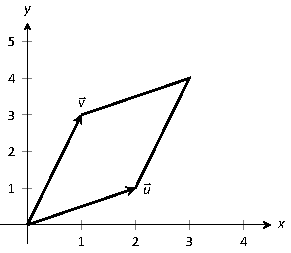
\includegraphics{figures/figcrossp4b}\\
	(a)\\[15pt]
	\myincludegraphicsthree{width=125pt,3Dmenu,activate=onclick,deactivate=onclick,
3Droll=0,
3Dortho=0.004,
3Dc2c=.42 .87 .26,
3Dcoo=61 60 63,
3Droo=250,
3Dlights=Headlamp,add3Djscript=asylabels.js}{scale=1.25,trim=4mm 5mm 4mm 5mm,clip=true}{figures/figcrossp4a}\\
	%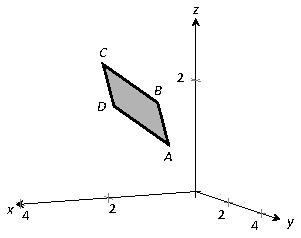
\includegraphics{figures/figcrossp4a}\\
	(b)
	\end{tabular}
	}
	\item		To show that the quadrilateral $ABCD$ is a parallelogram (shown in Figure \ref{fig:crossp4}(b)), we need to show that the opposite sides are parallel. We can quickly show that $\overrightarrow{AB} =\overrightarrow{DC} = \la 1,2,1\ra$ and $\overrightarrow{BC} = \overrightarrow{AD} = \la 2,2,1\ra$. We find the area by computing the magnitude of the cross product of $\overrightarrow{AB}$ and $\overrightarrow{BC}$:
\[
\overrightarrow{AB} \times \overrightarrow{BC} = \la 0,1,-2\ra \quad \Rightarrow \quad \norm{\overrightarrow{AB}\times\overrightarrow{BC}} = \sqrt{5} \approx 2.236.
\]
\end{enumerate}
\vskip-\baselineskip
}\\

This application is perhaps more useful in finding the area of a triangle (in short, triangles are used more often than parallelograms). We illustrate this in the following example.\\

\mfigure{.25}{Finding the area of a triangle in Example \ref{ex_crossp5}.}{fig:crossp5}{figures/figcrossp5}

\example{ex_crossp5}{Area of a triangle}{
Find the area of the triangle with vertices $A=(1,2)$, $B=(2,3)$ and $C=(3,1)$, as pictured in Figure \ref{fig:crossp5}.}
{We found the area of this triangle in Example \ref{ex_abc4} to be $1.5$ using integration. There we discussed the fact that finding the area of a triangle can be inconvenient using the ``$\frac12bh$'' formula as one has to compute the height, which generally involves finding angles, etc. Using a cross product is much more direct.

We can choose any two sides of the triangle to use to form vectors; we choose $\overrightarrow{AB} = \la 1,1\ra$ and $\overrightarrow{AC}=\la 2,-1\ra$. As in the previous example, we will rewrite these vectors with a third component of 0 so that we can apply the cross product. The area of the triangle is
\[
\frac12\norm{\overrightarrow{AB}\times\overrightarrow{AC}} = \frac12\norm{\la 1,1,0\ra \times \la 2,-1,0\ra} = \frac12\norm{\la 0,0,-3\ra} = \frac32.
\]
We arrive at the same answer as before with less work.
}\\



\pagebreak

\noindent\textbf{Volume of a Parallelepiped}

The three dimensional analogue to the parallelogram is the \textbf{parallelepiped}. Each face is parallel to the face opposite face, as illustrated in Figure \ref{fig:crossp_parallelepiped}. The volume of any three-dimensional solid whose cross-sectional area is a constant is given by $V=B\cdot h$, where $B$ is the area of the base (the constant cross-sectional area), and $h$ is the height. To determine a formula for the volume, we refer to Figure \ref{fig:parallelepiped_volume}. By crossing $\vec v$ and $\vec w$, one gets a vector whose magnitude is the area of the base, and whose direction is perpendicular to the parallelogram forming the base of the solid. We can then see that the height of the parallelepiped is equal to the length of the projection of the vector $\vec u$ onto $\crossp vw$. Thus, our volume is given by:
\begin{align*}
V & = B\cdot h\\
  & = \len{\crossp vw}\cdot \len{\operatorname{proj}_{\crossp vw}\vec{u}}\\
  & = \len{\crossp vw}\cdot\len{\left(\frac{\vec{u}\boldsymbol{\cdot}(\crossp vw)}{\len{\crossp vw}^2}\right)(\crossp vw)}\\
  & = \len{\crossp vw}\frac{\abs{\vec{u}\boldsymbol{\cdot}(\crossp vw)}}{\len{\crossp vw}^2}\len{\crossp vw}\\
  & = \abs{\vec{u}\boldsymbol{\cdot}(\crossp vw)}.
\end{align*}

\mfigurethree{width=75pt,3Dmenu,activate=onclick,deactivate=onclick,
3Droll=0,
3Dortho=0.0045,
3Dc2c=.84 .46 .26,
3Dcoo=0 110 86,
3Droo=150,
3Dlights=Headlamp,add3Djscript=asylabels.js}{}{.8}{A parallelepiped is the three dimensional analogue to the parallelogram.}{fig:crossp_parallelepiped}{figures/figcrosspparallelpiped}
%\mfigure{.53}{A parallelepiped is the three dimensional analogue to the parallelogram.}{fig:crossp_parallelepiped}{figures/figcrosspparallelpiped}
\index{cross product!applications!volume of parallelepiped}

Thus the volume of a parallelepiped defined by vectors $\vecu$, $\vecv$ and $\vec w$ is 
\begin{equation}
V = \abs{\vecu\boldsymbol{\cdot} (\crossp vw)}.\label{eq:crossp2}
\end{equation}
Note how this is the Scalar Triple Product, first seen in Theorem \ref{thm:cross_prod_prop}. Applying the identities given in the theorem shows that we can apply the Scalar Triple Product in any ``order'' we choose to find the volume. That is,
\[
V = |\vecu\boldsymbol{\cdot}(\crossp vw)| = |\vec u\boldsymbol{\cdot} (\crossp wv)| = |(\crossp uv)\boldsymbol{\cdot} \vecw|,\quad \text{etc.}
\]

\mfigure[width=0.95\marginparwidth]{.55}{Determining the volume of a parallelepiped}{fig:parallelepiped_volume}{figures/parallelepiped2}

\example{ex_crossp6}{Finding the volume of parallelepiped}{
Find the volume of the parallelepiped defined by the vectors $\vecu = \la 1,1,0\ra$, $\vecv = \la -1,1,0\ra$ and $\vecw = \la 0,1,1\ra$. 
}
{We apply Equation \eqref{eq:crossp2}. We first find $\crossp vw =\la 1,1,-1\ra$. Then
\[
|\vec u\cdot(\crossp vw)| = |\la 1,1,0\ra \cdot \la1,1,-1\ra| = 2.
\]
So the volume of the parallelepiped is 2 cubic units.
\mfigurethree{width=125pt,3Dmenu,activate=onclick,deactivate=onclick,
3Droll=0,
3Dortho=0.0045,
3Dc2c=4 4 2,
3Dcoo=0 50 50,
3Droo=150,
3Dlights=Headlamp,add3Djscript=asylabels.js}{}{.3}{A parallelepiped in Example \ref{ex_crossp6}.}{fig:crossp6}{figures/figcrossp6}
%\mfigure{.3}{A parallelepiped in Example \ref{ex_crossp6}.}{fig:crossp6}{figures/figcrossp6}
}\\

Let's take another look at how Equation \eqref{eq:crossp2} is computed in terms of our formulas for the dot and cross products. With $\vec u = \la u_1, u_2, u_3\ra, \vec v = \la v_1, v_2, v_3\ra$, and $\vec w = \la w_1, w_2, w_3\ra$, we have
\begin{align*}
\vec{u}\boldsymbol{\cdot}(\crossp vw) & = \la u_1, u_2, u_3\ra \boldsymbol{\cdot}\left\langle \bvm v_2 & v_3\\w_2&w_3\evm, -\bvm v_1 & v_3\\ w_1 & w_3\evm, \bvm v_1 & v_2\\ w_1 & w_2\evm\right\rangle\\
 & = u_1\bvm v_2 & v_3\\w_2&w_3\evm - u_2\bvm v_1 & v_3\\ w_1 & w_3\evm + u_3\bvm v_1 & v_2\\ w_1 & w_2\evm.
\end{align*}
Compare this with our determinant formula for computing the cross product,
\[
\crossp vw = \bvm \veci & \vecj & \veck\\ v_1 & v_2 & v_3\\ w_1 & w_2 & w_3\evm = \bvm v_2 & v_3\\w_2&w_3\evm\veci - \bvm v_1 & v_3\\ w_1 & w_3\evm\vecj + \bvm v_1 & v_2\\ w_1 & w_2\evm\veck.
\]
If we replace the unit vectors $\veci, \vecj, veck$ in the above equation with the components of $\vec{u}$, we arrive at our first instance of a \textbf{$3\times 3$ determinant}, along with a method for computing such an object:
\[
\bvm u_1 & u_2 & u_3\\ v_1 & v_2 & v_3\\ w_1 & w_2 & w_3\evm = u_1 \bvm v_2 & v_3\\ w_2 & w_3\evm - u_2\bvm v_1 & v_3\\ w_1 & w_3\evm + u_3\bvm v_1 & v_2\\ w_1 & w_2\evm = \vec u\boldsymbol{\cdot}(\crossp vw).
\]
We will return to our study of determinants in Section \ref{sec:determinant_1}, where we will learn techniques for efficiently computing determinants of any size.

While this application of the Scalar Triple Product is interesting, it is not used all that often: parallelepipeds are not a common shape in physics and engineering. (It is, however, essential to understanding the change of variables formula for multiple integrals in Calculus.) The last application of the cross product is very applicable in engineering.\\

\noindent\textbf{Torque}\\

\textbf{Torque} is a measure of the turning force applied to an object. A classic scenario involving torque is the application of a wrench to a bolt. When a force is applied to the wrench, the bolt turns. When we represent the force and wrench with vectors $\vec F$ and $\vec \ell$, we see that the bolt moves (because of the threads) in a  direction orthogonal to $\vec F$ and $\vec \ell$. Torque is usually represented by the Greek letter $\tau$, or tau, and has units of N$\cdot$m, a Newton--meter, or ft$\cdot$lb, a foot--pound.\index{cross product!applications!torque}

While a full understanding of torque is beyond the purposes of this book, when a force $\vec F$ is applied to a lever arm $\vec \ell$, the resulting torque is \begin{equation}\vec \tau = \crossp \ell F.\label{eq:crossp3}\end{equation}

\example{ex_crossp7}{Computing torque}{
A lever of length 2ft makes an angle with the horizontal of $45^\circ$. Find the resulting torque when a force of 10lb is applied to the end of the level where:
\begin{enumerate}
	\item the force is perpendicular to the lever, and
	\item	the force makes an angle of $60^\circ$ with the lever, as shown in Figure \ref{fig:crossp7}.
\end{enumerate}
}
{\begin{enumerate}
	\item We start by determining vectors for the force and lever arm. Since the lever arm makes a $45^\circ$ angle with the horizontal and is 2ft long, we can state that $\vec \ell = 2\la \cos 45^\circ,\sin 45^\circ\ra = \la \sqrt2,\sqrt2\ra.$
	
	Since the force vector is perpendicular to the lever arm (as seen in the left hand side of Figure \ref{fig:crossp7}), we can conclude it is making an angle of $-45^\circ$ with the horizontal. As it has a magnitude of 10lb, we can state $\vec F = 10\la \cos (-45^\circ), \sin(-45^\circ)\ra = \la 5\sqrt2,-5\sqrt2\ra.$
	
	Using Equation \eqref{eq:crossp3} to find the torque requires a cross product. We again let the third component of each vector be 0  and compute the cross product:
	\begin{align*}
	\vec\tau &= \crossp \ell F \\
				&= \la \sqrt2,\sqrt2,0\ra \times \la 5\sqrt2,-5\sqrt2,0\ra \\
				&= \la 0,0,-20\ra
	\end{align*}
	This clearly has a magnitude of 20 ft-lb.
	
	We can view the force and lever arm vectors as lying ``on the page''; our computation of $\vec\tau$ shows that the torque goes ``into the page.'' This follows the Right Hand Rule of the cross product, and it also matches well with the example of the wrench turning the bolt. Turning a bolt clockwise moves it in.
	
	\item		Our lever arm can still be represented by $\vec \ell = \la \sqrt2,\sqrt2\ra$. As our force vector makes a $60^\circ$ angle with $\vec \ell$, we can see (referencing the right hand side of the figure) that $\vec F$ makes a $-15^\circ$ angle with the horizontal. Thus 
	\begin{align*}
	\vec F = 10\la \cos-15^\circ,\sin-15^\circ\ra &= \la \frac{5(1+\sqrt3)}{\sqrt2},-\frac{5(1+\sqrt3)}{\sqrt2}\ra \\
	&\approx \la 9.659,-2.588\ra.\end{align*}
	
	We again make the third component 0 and take the cross product to find the torque:
	\begin{align*}
	\vec\tau &= \crossp \ell F\\
					&= \la \sqrt2,\sqrt2,0\ra \times  \la \frac{5(1+\sqrt3)}{\sqrt2},-\frac{5(1+\sqrt3)}{\sqrt2},0\ra\\
					&= \la 0,0,-10\sqrt3\ra\\
					&\approx \la 0,0,-17.321\ra.
	\end{align*}
	As one might expect, when the force and lever arm vectors \textit{are} orthogonal, the magnitude of force is greater than when the vectors \textit{are not} orthogonal.
\end{enumerate}
\vskip-\baselineskip
}\\

\mfigure{.6}{Showing a force being applied to a lever in Example \ref{ex_crossp7}.}{fig:crossp7}{figures/figcrossp7}

While the cross product has a variety of applications (as noted in this chapter), its fundamental use is finding a vector perpendicular to two others. Knowing a vector is orthogonal to two others is of incredible importance, as it allows us to find the equations of lines and planes in a variety of contexts. The importance of the cross product, in some sense, relies on the importance of lines and planes, which see widespread use throughout engineering, physics and mathematics. We study lines and planes in the next two sections. 

\printexercises{exercises/10_04_exercises}


\section{Lines}\label{sec:lines}

\index{lines}
To find the equation of a line in the $x$-$y$ plane, we need two pieces of information: a point and the slope. The slope conveys \textit{direction} information. As vertical lines have an undefined slope, the following statement is more accurate:

\begin{quotation}
\noindent To define a line, one needs a point on the line and the direction of the line.
\end{quotation}

This holds true for lines in space.\\

Let $P$ be a point in space, let $\vec p$ be the vector with initial point at the origin and terminal point at $P$ (i.e., $\vec p$ ``points'' to $P$), and let $\vec d$ be a vector. Consider the points on the line through $P$ in the direction of $\vec d$. 

Clearly one point on the line is $P$; we can say that the \emph{vector} $\vec p$ lies at this point on the line. To find another point on the line, we can start at $\vec p$ and move in a  direction parallel to $\vec d$. For instance, starting at $\vec p$ and traveling one length of $\vec d$ places one at another point on the line. Consider Figure \ref{fig:lines_intro} where certain points along the line are indicated. 
\mfigurethree{width=125pt,3Dmenu,activate=onclick,deactivate=onclick,
3Droll=0,
3Dortho=0.0045,
3Dc2c=.84 .46 .26,
3Dcoo=0 70 0,
3Droo=150,
3Dlights=Headlamp,add3Djscript=asylabels.js}{scale=1.25,trim=5mm 5mm 5mm 5mm,clip=true}{.7}{Defining a line in space.}{fig:lines_intro}{figures/figlines_intro}
%\mfigure[scale=1.25,trim=5mm 5mm 5mm 5mm,clip=true]{.7}{Defining a line in space.}{fig:lines_intro}{figures/figlines_intro}

The figure illustrates how every point on the line can be obtained by starting with $\vec p$ and moving a certain distance in the direction of $\vec d$. That is, we can define the line as a function of $t$:
\begin{equation}\vec\ell(t) = \vec p + t\ \vec d.\label{eq:lines1}\end{equation}

In many ways, this is \textit{not} a new concept. Compare Equation \eqref{eq:lines1} to the familiar ``$y=mx+b$'' equation of a line:

\begin{center}
\begin{tikzpicture}[>=stealth]
	\draw (0,0) node (L) {\large $y\ =\ b\ +\ m\,x$};
	\draw (5,0) node (R) {\large $\vec \ell(t)\ =\ \vec p\ +\ t\,\vec d$};
\node (A) at (1,1.5) [align=center,] {Starting\\ Point};
\node (B) at (4,1.5) [align=center] {Direction};
\node (C) at (2.5,-1.5) [align=center] {How Far To\\  Go In That \\Direction};
\draw [->,thick] (A) -- ($(R)+(-1pt,8pt)$);	
\draw [->,thick] (A) -- ($(L)+(-0pt,10pt)$);
\draw [->,thick] (B) -- (.9,.2);
\draw [->,thick] (B) -- ($(R)+(30pt,7pt)$);
\draw [->,thick] (C) -- (1.3,-.15);
\draw [->,thick] (C) -- ($(R)+(25pt,-7pt)$);
\end{tikzpicture}
\captionsetup{type=figure}%
\caption{Understanding the vector equation of a line.}
\label{fig:lines_eq}
\end{center}


%\begin{center}
%\begin{tikzpicture}[>=stealth]
	%\draw (0,0) node {\large $y\ =\ b\ +\ m\,x$};
%\node (A) at (-1,-1) [align=center,] {Starting\\ Point};
%\node (B) at (1,-1) [align=center] {Direction};
%\node (C) at (3,-1) [align=center] {How Far To\\  Go In That \\Direction};
%\draw [->,thick] (A) -- (-.3,-.2);	
%\draw [->,thick] (B) -- (.8,-.2);
%\draw [->,thick] (C) -- (1.3,-.15);
%\end{tikzpicture}
%\end{center}
%Now compare this to the formula given in Equation \eqref{eq:lines1}:
%\begin{center}
%\begin{tikzpicture}[>=stealth]
	%\draw (0,0) node {\large $\vec \ell(t)\ =\ \vec p\ +\ t\,\vec d$};
%\node (A) at (-1,-1) [align=center,] {Starting\\ Point};
%\node (B) at (.5,.75) [align=center] {Direction};
%\node (C) at (2,-1.25) [align=center] {How Far To\\  Go In That \\Direction};
%\draw [->,thick] (A) -- (-.05,-.2);	
%\draw [->,thick] (B) -- (1.2,.3);
%\draw [->,thick] (C) -- (1.0,-.2);
%\end{tikzpicture}
%\end{center}

The equations exhibit the same structure: they give a starting point, define a direction, and state how far in that direction to travel.

Equation \eqref{eq:lines1} is an example of a \textbf{vector--valued function}; the input of the function is a real number and the output is a vector. We will cover vector--valued functions extensively in the next chapter.

There are other ways to represent a line. Let $\vec p = \la x_0,y_0,z_0\ra$ and let $\vec d = \la a,b,c\ra$. Then the equation of the line through $\vec p$ in the direction of $\vec d$ is:
\begin{align*}
\vec\ell(t) &= \vec p + t\vec d \\
						&= \la x_0,y_0,z_0\ra + t\la a,b,c\ra \\
						&= \la x_0 + at, y_0+bt, z_0+ct\ra.
\end{align*}

The last line states the the $x$ values of the line are given by $x=x_0+at$, the $y$ values are given by $y = y_0+bt$, and the $z$ values are given by $z = z_0 + ct$. These three equations, taken together, are the \textbf{parametric equations of the line} through $\vec p$ in the direction of $\vec d$.

Finally, each of the equations for $x$, $y$ and $z$ above contain the variable $t$. We can solve for $t$ in each equation:
\begin{align*}
x = x_0+at \quad&\Rightarrow\quad t=\frac{x-x_0}{a},\\
y=y_0+bt \quad&\Rightarrow\quad t = \frac{y-y_0}{b},\\
z = z_0+ct \quad&\Rightarrow\quad t = \frac{z-z_0}{c},\\
\end{align*}
assuming $a,b,c\neq 0$.
Since $t$ is equal to each expression on the right, we can set these equal to each other, forming the \textbf{symmetric equations of the line} through $\vec p$ in the direction of $\vec d$:
\[
\frac{x-x_0}{a} = \frac{y-y_0}{b}=\frac{z-z_0}{c}.
\]
Each representation has its own advantages, depending on the context. We summarize these three forms in the following definition, then give examples of their use.
%\clearpage

\definition{def:lines}{Equations of Lines in Space}
{Consider the line in space that passes through $\vec p = \la x_0,y_0,z_0\ra$ in the direction of $\vec d = \la a,b,c\ra.$\index{lines!equations for}
\begin{enumerate}
	\item The \textbf{vector equation} of the line is 
	\[
	\vec \ell(t) = \vec p+t\vec d.
	\]
	\item	The \textbf{parametric equations} of the line are
	\[
	x = x_0+at, \quad y=y_0+bt, \quad z = z_0+ct .
	\]
	\item	The \textbf{symmetric equations} of the line are
	\[
	\frac{x-x_0}{a} = \frac{y-y_0}{b}=\frac{z-z_0}{c}.
	\]
\end{enumerate}
}

\example{ex_lines1}{Finding the equation of a line}{
Give all three equations, as given in Definition \ref{def:lines}, of the line through $P = (2,3,1)$ in the direction of $\vec d = \la -1,1,2\ra$. Does the point $Q=(-1,6,6)$ lie on this line?}
{We identify the point $P=(2,3,1)$ with the vector $\vec p =\la 2,3,1\ra$. Following the definition, we have
\begin{itemize}
	\item the vector equation of the line is $\vec\ell(t) = \la 2,3,1\ra + t\la -1,1,2\ra$;
	\item	the parametric equations of the line are
	\[
	x = 2-t,\quad y = 3+t,\quad z = 1+2t; \text{ and}
	\]
	\item	the symmetric equations of the line are
	\[
	\frac{x-2}{-1}=\frac{y-3}{1} = \frac{z-1}{2}.
	\]
\end{itemize}
\mfigurethree{width=125pt,3Dmenu,activate=onclick,deactivate=onclick,
3Droll=0,
3Dortho=0.0045,
3Dc2c=.78 .53 .32,
3Dcoo=0 70 50,
3Droo=150,
3Dlights=Headlamp,add3Djscript=asylabels.js}{scale=1.25,trim=2mm 2mm 2mm 2mm,clip=true}{.2}{Graphing a line in Example \ref{ex_lines1}.}{fig:lines1}{figures/figlines1}
%\mfigure[scale=1.25,trim=2mm 2mm 2mm 2mm,clip=true]{.5}{Graphing a line in Example \ref{ex_lines1}.}{fig:lines1}{figures/figlines1}

The first two equations of the line are useful when a $t$ value is given: one can immediately find the corresponding point on the line. These forms are good when calculating with a computer; most software programs easily handle equations in these formats. (For instance, to make Figure \ref{fig:lines1}, a certain graphics program was given the input \texttt{(2-x,3+x,1+2*x)}. This particular program requires the variable always be ``$x$'' instead of ``$t$'').

Does the point $Q = (-1,6,6)$ lie on the line? The graph in Figure \ref{fig:lines1} makes it clear that it does not. We can answer this question without the graph using any of the three equation forms. Of the three, the symmetric equations are probably best suited for this task. Simply plug in the values of $x$, $y$ and $z$ and see if equality is maintained:
\[
 \frac{-1-2}{-1} \stackrel{?}{=} \frac{6-3}{1} \stackrel{?}{=} \frac{6-1}{2} \quad \Rightarrow \quad 3=3\neq2.5.
 \]
We see that $Q$ does not lie on the line as it did not satisfy the symmetric equations.
}\\

\example{ex_lines6}{Finding the equation of a line through two points}{
Find the parametric equations of the line through the points $P=(2,-1,2)$ and $Q = (1,3,-1)$.}
{Recall the statement made at the beginning of this section: to find the equation of a line, we need a point and a direction. We have \emph{two} points; either one will suffice. The direction of the line can be found by the vector with initial point $P$ and terminal point $Q$: $\overrightarrow{PQ} = \la -1,4,-3\ra$.

The parametric equations of the line $\ell$ through $P$ in the direction of $\overrightarrow{PQ}$ are:
\[
\ell: \quad x= 2-t\quad y=-1+4t \quad z=2-3t.
\]
\mfigurethree{width=125pt,3Dmenu,activate=onclick,deactivate=onclick,
3Droll=0,
3Dortho=0.0045,
3Dc2c=.4 .87 .32,
3Dcoo=58 8.7 4.6,
3Droo=150,
3Dlights=Headlamp,add3Djscript=asylabels.js}{scale=1.25}{.5}{A graph of the line in Example \ref{ex_lines6}.}{fig:lines6}{figures/figlines6}
%\mfigure[scale=1.25]{.6}{A graph of the line in Example \ref{ex_lines6}.}{fig:lines6}{figures/figlines6}

A graph of the points and line are given in Figure \ref{fig:lines6}. Note how in the given parametrization of the line, $t=0$ corresponds to the point $P$, and $t=1$ corresponds to the point $Q$. This relates to the understanding of the vector equation of a line described in Figure \ref{fig:lines_eq}. The parametric equations ``start'' at the point $P$, and $t$ determines how far in the direction of $\overrightarrow{PQ}$ to travel. When $t=0$, we travel 0 lengths of $\overrightarrow{PQ}$; when $t=1$, we travel one length of $\overrightarrow{PQ}$, resulting in the point $Q$.
}\\

\noindent \textbf{\large Parallel, Intersecting and Skew Lines}\\

In the plane, two \emph{distinct} lines can either be parallel or they will intersect at exactly one point. In space, given equations of two lines, it can sometimes be difficult to tell whether the lines are distinct or not (i.e., the same line can be represented in different ways). Given lines $\vec\ell_1(t) = \vec p_1 + t\vec d_1$ and $\vec \ell_2(t) = \vec p_2+t\vec d_2$, we have four possibilities: $\vec \ell_1$ and $\vec \ell_2$ are
\index{lines!skew}\index{lines!parallel}\index{lines!intersecting}

\begin{center}
\begin{tabular}{p{100pt}p{150pt}}
the same line & they share all points; \\
intersecting lines & share only 1 point;\\
parallel lines & $\vec d_1\parallel \vec d_2$, no points in common; or \\
skew lines & $\vec d_1\nparallel \vec d_2$, no points in common. 
\end{tabular}
\end{center}

The next two examples investigate these possibilities.\\

\example{ex_lines2}{Comparing lines}{
Consider lines $\ell_1$ and $\ell_2$, given in parametric equation form:
\[
\ell_1: \begin{array}{ccc} x&=&1+3t \\ y&=&2-t\\z&=&t\end{array}\qquad\qquad \ell_2:\begin{array}{ccc} x&=&-2+4s\\y&=&3+s\\z&=&5+2s.\end{array}
\]
Determine whether $\ell_1$ and $\ell_2$ are the same line, intersect, are parallel, or skew.}
{We start by looking at the directions of each line. Line $\ell_1$ has the direction given by $\vec d_1=\la 3,-1,1\ra$ and line $\ell_2$ has the direction given by $\vec d_2 = \la 4,1,2\ra$. It should be clear that $\vec d_1$ and $\vec d_2$ are not parallel, hence $\ell_1$ and $\ell_2$ are not the same line, nor are they parallel. Figure \ref{fig:lines2} verifies this fact (where the points and directions indicated by the equations of each line are identified).
\mfigurethree{width=125pt,3Dmenu,activate=onclick,deactivate=onclick,
3Droll=0,
3Dortho=0.0045,
3Dc2c=.42 .80 .43,
3Dcoo=0 30 50,
3Droo=150,
3Dlights=Headlamp,add3Djscript=asylabels.js}{scale=1.25,trim=5mm 5mm 5mm 5mm,clip=true}{.6}{Sketching the lines from Example \ref{ex_lines2}.}{fig:lines2}{figures/figlines2}
%\mfigure[scale=1.25,trim=5mm 5mm 5mm 5mm,clip=true]{.6}{Sketching the lines from Example \ref{ex_lines2}.}{fig:lines2}{figures/figlines2}

We next check to see if they intersect (if they do not, they are skew lines). To find if they intersect, we look for $t$ and $s$ values such that the respective $x$, $y$ and $z$ values are the same. That is, we want $s$ and $t$ such that:
\[
\begin{array}{ccccc}
1+3t &=&x&=&-2+4s\\
2-t&=&y&=&3+s\\
t&=&z&=&5+2s.
\end{array}
\]
This is a relatively simple system of linear equations. Since the last equation is already solved for $t$, substitute that value of $t$ into the equation above it:
\[
2-(5+2s) = 3+s \quad \Rightarrow \quad s=-2,\ t=1.
\]
A key to remember is that we have \emph{three} equations; we need to check if $s=-2,\ t=1$ satisfies the first equation as well:
\[
1+3(1) \neq -2+4(-2).
\]
It does not. Therefore, we conclude that the lines $\ell_1$ and $\ell_2$ are skew.
}\\

\mnote{.4}{We say that a system of equations with no solution, such as the one in Example \ref{ex_lines2}, is \textit{inconsistent}. Although it is possible to find values that work for any two of the three equations, there is no set of values for $s$ and $t$ that work for all three equations simultaneously. We'll develop general techniques for studying systems of linear equations in Chapter \ref{chapter:linear}.}

\example{ex_lines8}{Comparing lines}{
Consider the lines $\ell_1$ and $\ell_2$ given by the vector equations
\begin{align*}
\vec\ell_1(s) & = \langle 2, -1, 4\rangle + s\langle 0, 4, -8\rangle\\
\vec\ell_2(t) & = \langle -3, 4, -6\rangle + t\langle 2, -1, 2\rangle.
\end{align*}
Determine if the lines are parallel, skew, or intersecting.}
{We can immediately see that the lines cannot be parallel, since the $x$-component of the direction vector for $\ell_1$ is zero, but this is not the case for the direction vector of $\ell_2$. (There is no scalar $c$ such that $c(0)=2$.) To determine if the lines intersect, we proceed as in the previous example. We must have
\[
\begin{array}{ccccc}
2 & = & x & = &-3+2t\\
-1+4s & = &  y & = & 4-t\\
4-8s & = & z & = & -6+2t.
\end{array}
\]
The first equation immediately gives us $2t=5$, so $t=\frac{5}{2}$. Plugging this into the second equation gives us
\[
4s = 4-\frac{5}{2}+1 = \frac{5}{2} \quad \Rightarrow \quad s=\frac{5}{8}.
\]
We now need to check to see if these values satisfy the third equation as well: we have
\[
4-8s = 4-5=-1,
\]
and
\[
-6+2t = -6+5=-1,
\]
so the values $s=\frac{5}{8}$, $t=\frac{5}{2}$ work for all three equations, and since
\begin{align*}
\vec\ell_1\left(\frac{5}{8}\right) &= \langle 2, -1, 4\rangle +\frac{5}{8}\langle 0, 4, -8\rangle = \langle 2, \frac{3}{2}, -1\rangle \tag*{and}\\
\vec\ell_2\left(\frac{5}{2}\right) & = \langle -3, 4, -6\rangle+\frac{5}{2}\langle 2, -1, 2\rangle = \langle 2, \frac{3}{2}, -1\rangle,
\end{align*}
our point of intersection is $(2, \frac{3}{2}, -1)$.
}\\


\example{ex_lines3}{Comparing lines}{
Consider lines $\ell_1$ and $\ell_2$, given in parametric equation form:
\[
\ell_1: \begin{array}{ccc} x&=&-0.7+1.6t \\ y&=&4.2+2.72t\\z&=&2.3-3.36t\end{array}\qquad\qquad \ell_2:\begin{array}{ccc} x&=&2.8-2.9s\\y&=&10.15-4.93s\\z&=&-5.05+6.09s.\end{array}
\]
Determine whether $\ell_1$ and $\ell_2$ are the same line, intersect, are parallel, or skew.}
{It is obviously very difficult to simply look at these equations and discern anything. This is done intentionally. In the ``real world,'' most equations that are used do not have nice, integer coefficients. Rather, there are lots of digits after the decimal and the equations can look ``messy.''

We again start by deciding whether or not each line has the same direction. The direction of $\ell_1$ is given by $\vec d_1 = \la 1.6,2.72,-3.36\ra$ and the direction of $\ell_2$ is given by $\vec d_2 = \la -2.9,-4.93,6.09\ra$. When it is not clear through observation whether two vectors are parallel or not, the standard way of determining this is by comparing their respective unit vectors. Using a calculator, we find:
\begin{align*}
\vec u_1 &= \frac{\vec d_1}{\norm{\vec d_1}} = \la 0.3471,0.5901,-0.7289\ra\\
 \vec u_2 &= \frac{\vec d_2}{\norm{\vec d_2}} = \la -0.3471,-0.5901,0.7289\ra.
\end{align*}

%\enlargethispage{\baselineskip}
The two vectors seem to be parallel (at least, their components are equal to 4 decimal places). In most situations, it would suffice to conclude that the lines are at least parallel, if not the same. One way to be sure is to rewrite $\vec d_1$ and $\vec d_2$ in terms of fractions, not decimals. We have 
\[
\vec d_1 =\la \frac{16}{10},\frac{272}{100},-\frac{336}{100}\ra \qquad \vec d_2 = \la -\frac{29}{10},-\frac{493}{100},\frac{609}{100}\ra.
\]
One can then find the magnitudes of each vector in terms of fractions, then compute the unit vectors likewise. After a lot of manual arithmetic (or after briefly using a computer algebra system), one finds that 
\[
\vec u_1 = \la \sqrt{\frac{10}{83}},\frac{17}{\sqrt{830}},-\frac{21}{\sqrt{830}}\ra \qquad \vec u_2 = \la -\sqrt{\frac{10}{83}},-\frac{17}{\sqrt{830}},\frac{21}{\sqrt{830}}\ra.
\]
We can now say without equivocation that these lines are parallel.

Are they the same line? The parametric equations for a line describe one point that lies on the line, so we know that the point $P_1 = (-0.7,4.2,2.3)$ lies on $\ell_1$. To determine if this point also lies on $\ell_2$, plug in the $x$, $y$ and $z$ values of $P_1$ into the symmetric equations for $\ell_2$:

\[
\begin{array}{ccccc}
\frac{(-0.7)-2.8}{-2.9} &\stackrel{?}{=}& \frac{(4.2)-10.15}{-4.93} &\stackrel{?}{=}& \frac{(2.3)-(-5.05)}{6.09}\\
 1.2069 &=& 1.2069 &=& 1.2069.
\end{array}
\]

\mfigurethree{width=125pt,3Dmenu,activate=onclick,deactivate=onclick,
3Droll=0,
3Dortho=0.0045,
3Dc2c=.56 .8 .22,
3Dcoo=0 0 0,
3Droo=150,
3Dlights=Headlamp,add3Djscript=asylabels.js}{scale=1.25,trim=2mm 0mm 0mm 0mm,clip=true}{.6}{Graphing the lines in Example \ref{ex_lines3}.}{fig:lines3}{figures/figlines3}
%\mfigure[scale=1.25,trim=2mm 0mm 0mm 0mm,clip=true]{.35}{Graphing the lines in Example \ref{ex_lines3}.}{fig:lines3}{figures/figlines3}
The point $P_1$ lies on both lines, so we conclude they are the same line, just parametrized differently. Figure \ref{fig:lines3} graphs this line along with the points and vectors described by the parametric equations. Note how $\vec d_1$ and $\vec d_2$ are parallel, though point in opposite directions (as indicated by their unit vectors above). 
}\\

\noindent\textbf{\large Distances}\\

Given a point $Q$ and a line $\vec\ell(t) = \vec p+t\vec d$ in space, it is often useful to know the distance from the point to the line. (Here we use the standard definition of ``distance,'' i.e., the length of the shortest line segment from the point to the line.) Identifying $\vec p$ with the point $P$, Figure \ref{fig:lines_dist1} will help establish a general method of computing this distance $h$.

\mfigure{.25}{Establishing the distance from a point to a line.}{fig:lines_dist1}{figures/figlines_dist1}

From trigonometry, we know $h = \norm{\overrightarrow{PQ}}\sin\theta$. We have a similar identity involving the cross product: $\norm{\overrightarrow{PQ}\times \vec d} = \norm{\overrightarrow{PQ}}\, \vnorm{d}\sin\theta.$ Divide both sides of this latter equation by $\vnorm{d}$ to obtain $h$:
\begin{equation}
h = \frac{\norm{\overrightarrow{PQ}\times \vec d}}{\vnorm{d}}.
\label{eq:lines2}
\end{equation}

We put Equation \eqref{eq:lines2} to use in the following example.\\

\example{ex_lines4}{Finding the distance from a point to a line}{
Find the distance from the point $Q=(1,1,3)$ to the line $\vec\ell(t) = \la 1,-1,1\ra+t\la 2,3,1\ra.$}
{The equation of the line line gives us the point $P=(1,-1,1)$ that lies on the line, hence $\overrightarrow{PQ} = \la 0,2,2\ra$. The equation also gives $\vec d= \la 2,3,1\ra$. Using Equation \eqref{eq:lines2}, we have the distance as 
\begin{align*}
h &= \frac{\norm{\overrightarrow{PQ}\times \vec d}}{\vnorm{d}}\\
	&= \frac{\norm{\la -4,4,-4\ra}}{\sqrt{14}}\\
	&=\frac{4\sqrt{3}}{\sqrt{14}}.
\end{align*}
}\\

While Equation \eqref{eq:lines2} gives us a convenient formula for computing the distance, you are probably better off making sure you understand the argument used to obtain the formula. For one thing, a formula is easily forgotten. For another, understanding the method will allow you to adapt it to similar situations still to come, such as computing the distance between skew lines, or from a point to a plane. The general method for these types of problems can be outlined as follows.

\keyidea{idea:distance_method}{Steps for solving shortest distance problems}{
Suppose you are asked to find the distance between two objects, or to determine an object (such as a point) that is closest to a given object (a line or plane). Your solution to the problem should always include the following steps:
\begin{enumerate}
\item Make a list of all the information provided in the problem.
\item Make a note of what quantities you're asked to determine.
\item \textbf{Draw a diagram}. Label all relevant points and vectors, including those you know, and those you want to find.
\item Using your diagram as a reference, compute any unknown points or vectors.
\end{enumerate}
}

\mnote{.6}{\textbf{Note:} We can't overemphasize the fact that the diagram referred to in Key Idea \ref{idea:distance_method} \textbf{does not have to be accurate} with respect to the coordinates and directions involved. It simply has to be capable of representing the information in the problem. Note that in Figure \ref{fig:linedistsetup} in Example \ref{ex_lines4a} we've drawn a line, some points, and some vectors that represent the problem, without reference to a coordinate system. The goal is to provide enough detail to allow us to set up the problem.}

We put the method in Key Idea \ref{idea:distance_method} to use in the following example. Note that in this example we're asked not just for the distance from a point to a line, but also for the point on the line that is \textit{closest} to the given point, so simply using Equation \eqref{eq:lines2} is not enough.

\mfigure{.4}{Setting up the solution in Example \ref{ex_lines4a}}{fig:linedistsetup}{figures/pointlinedist}

\example{ex_lines4a}{Finding the closest point on a line}{
Find the distance from the point $Q=(1,3,-2)$ to the line $\vec\ell$ that passes through the point $P=(2,0,-1)$ in the direction of $\vec d = \la 1,-1,0\ra$, and find the point $R$ on $\vec\ell$ that is closest to $Q$.}
{We're given a point $P$ on the line, along with a direction vector $\vec d$, and a point $Q$ not on the line. We seek the point $R$ on the line that is closest to $Q$, as well as the distance from $Q$ to $R$. We begin by diagramming the information in Figure \ref{fig:linedistsetup}. From the given points $P$ and $Q$ we can immediately construct the vector
\[
\overrightarrow{PQ}=\la 1-2, 3-0, -2-(-1)\ra = \la -1, 3, -1\ra.
\]
Rather than use Formula \eqref{eq:lines2} to find the distance, we begin instead by finding the point $R$ on the line that is closest to $Q$. From our diagram, we can see that the vector $\overrightarrow{PR}$ from $P$ to $R$ is equal to the projection of $\overrightarrow{PQ}$ onto the distance vector $\vec{d}$:
\[
\overrightarrow{PR}=\operatorname{proj}_{\vec{d}}\overrightarrow{PQ}= \left(\frac{\la -1,3,-1\ra\boldsymbol{\cdot}\la 1,-1,0\ra}{\la 1,-1,0\ra\boldsymbol{\cdot}\la 1,-1,0\ra}\right)\la 1,-1,0\ra = \la -2,2,0\ra.
\]
Now, we need to pause and take care that we don't make a very common mistake: the vector $\overrightarrow{PR}$ does \textbf{not} give the coordinates of the point $R$. Instead, $\overrightarrow{PR}$ tells us how to get \textit{from} the point $P$ \textit{to} the point $R$. Letting $O$ denote the origin, we can write $\overrightarrow{OP}$ and $\overrightarrow{OR}$ for the position vectors of $P$ and $R$, respectively. Since $\overrightarrow{PR} = \overrightarrow{OR}-\overrightarrow{OP}$ using the ``tip minus tail'' rule for computing the vector between two points, we have
\[
\overrightarrow{OR} = \overrightarrow{OP}+\overrightarrow{PR} = \la 2, 0, -1\ra + \la -2, 2, 0\ra = \la 0, 2, -1\ra.
\]
Thus, we have $R=(0,2,-1)$ as the point on the line closest to the point $Q$. We can now find the distance from $Q$ to the line using the distance formula:
\[
D= \sqrt{(1-0)^2+(3-2)^2+(-2-(-1))^2} = \sqrt{3}.
\]
(You should verify that this agrees with the distance given by Formula \eqref{eq:lines2}.)
An alternative way of computing the distance is to make use of the orthogonal decomposition in Key Idea \ref{idea:orthog_proj}. By definition of the distance from a point to a line, we know that the vector $\overrightarrow{RQ}$ must be orthogonal to the line, and thus to the direction vector $\vec{d}$. Using Key Idea \ref{idea:orthog_proj}, we have that
\[
\overrightarrow{RQ}= \overrightarrow{PQ}-\overrightarrow{PR} = \la -1, 3, -1\ra - \la -2, 2, 0\ra = \la -1, 1, 1\ra,
\]
and the shortest distance is given by $\len{\overrightarrow{RQ}}=\sqrt{3}$, as before.
}\\

It is also useful to determine the distance between lines, which we define as the length of the shortest line segment that connects the two lines. This line segment is necessarily perpendicular to both lines. Let lines $\vec\ell_1(t) = \vec p_1 + t\vec d_1$ and $\vec\ell_2(t) = \vec p_2 + t\vec d_2$ be given, as shown in Figure \ref{fig:lines_dist2}. To find the direction orthogonal to both $\vec d_1$ and $\vec d_2$, we take the cross product: $\vec c = \vec d_1\times \vec d_2$. The magnitude of the orthogonal projection of $\overrightarrow{P_1P_2}$ onto $\vec c$ is the distance $h$ we seek:
\begin{align}
h&=		\snorm{\text{proj}\,_{\vec c}\,\overrightarrow{P_1P_2}} = \snorm{\frac{\overrightarrow{P_1P_2}\cdot\vec c}{\dotp cc}\vec c} \nonumber\\
	&=\frac{\lvert\overrightarrow{P_1P_2}\cdot \vec c\rvert}{\vnorm c^2}\vnorm c =\frac{\abs{\overrightarrow{P_1P_2}\cdot \vec c}}{\vnorm c}.\label{eq:skewlinesdist}
\end{align}
A problem in the Exercise section is to show that this distance is 0 when the lines intersect. Note the use of the Triple Scalar Product: $\overrightarrow{P_1P_2}\cdot c = \overrightarrow{P_1P_2}\cdot (\vec d_1\times \vec d_2).$\\

\mnote{.25}{\textbf{Note:} Skew lines always lie in parallel \textit{planes}. In the next section we'll see that a plane can be determined by two non-parallel direction vectors and a point on the plane. The distance between the two skew lines is then equal to the distance between the two parallel planes, which is given by the length of a line segment perpendicular to both planes, and therefore, to both lines.}

\mfigurethree{width=125pt,3Dmenu,activate=onclick,deactivate=onclick,
3Droll=6.34,
3Dortho=0.0076,
3Dc2c=.009 -.76 .65,
3Dcoo=2.92 11.35 23.78,
3Droo=150,
3Dlights=Headlamp,add3Djscript=asylabels.js}{}{.45}{Establishing the distance between lines.}{fig:lines_dist2}{figures/figlines_dist2}
%\mfigure{.45}{Establishing the distance between lines.}{fig:lines_dist2}{figures/figlines_dist2}

%The following Key Idea restates these two distance formulas.

%\keyidea{idea:line_distance}{Distances to Lines}
%{\begin{enumerate}
%	\item Let $P$ be a point on a line $\ell$ that is parallel to $\vec d$. The distance $h$ from a point $Q$ to the line $\ell$ is:
%	\index{distance!between point and line}\index{distance!between lines}\index{lines!distances between}
%	\[
%	h =\frac{\norm{\overrightarrow{PQ}\times \vec d}}{\vnorm{d}}.
%	\]
%	\item	Let $P_1$ be a point on line $\ell_1$ that is parallel to $\vec d_1$, and let $P_2$ be a point on line $\ell_2$ parallel to $\vec d_2$, and let $\vec c = \vec d_1\times \vec d_2$, where lines $\ell_1$ and $\ell_2$ are not parallel. The distance $h$ between the two lines is:
%	\[
%	h=\frac{|\overrightarrow{P_1P_2}\cdot \vec c|}{\vnorm c}.
%	\]
%\end{enumerate}
%}



\example{ex_lines5}{Finding the distance between lines}{
Find the distance between the lines 
\[
\ell_1: \begin{array}{ccc} x&=&1+3t \\ y&=&2-t\\z&=&t\end{array}\qquad\qquad \ell_2:\begin{array}{ccc} x&=&-2+4s\\y&=&3+s\\z&=&5+2s.\end{array}
\]
}
{These are the sames lines as given in Example \ref{ex_lines2}, where we showed them to be skew. The equations allow us to identify the following points and vectors:
\begin{align*}
P_1 = (1,2,0)\quad P_2 &= (-2,3,5) \quad \Rightarrow \quad \overrightarrow{P_1P_2} = \la -3,1,5\ra.\\
\vec d_1 = \la 3,-1,1\ra \quad \vec d_2 &= \la 4,1,2\ra \quad \Rightarrow \quad \vec c = \vec d_1\times \vec d_2 = \la -3,-2,7\ra.
\end{align*}
Using Equation \eqref{eq:skewlinesdist} we have that the distance $h$ between the two lines is
\[
h = \frac{|\overrightarrow{P_1P_2}\cdot \vec c|}{\vnorm c}=\frac{42}{\sqrt{62}}\approx 5.334.
\]
}\\

Once again, we do not recommend attempting to memorize Equation \eqref{eq:skewlinesdist}. Unless you somehow find yourself at a point in your life where you need to find the distances between a whole lot of pairs of skew lines, you will be better served by learning the skills required to set up and think through a problem than you will be by memorizing a formula to plug numbers into. In the case of skew lines, the key observation is that if we take the vector between \textbf{any} pair of points, one on each line, and project it onto the vector $\vec c = \vec{d}_1\times\vec{d}_2$, the length of the resulting vector is the distance we seek.

Somewhat more challenging is the problem of finding the points on each line that actually \textit{realize} this shortest distance.\\

\example{ex_lines7}{Finding the closest points on skew lines}{
Find the points $R_1$ on $\vec\ell_1$ and $R_2$ on $\vec\ell_2$, where $\vec\ell_1$ and $\vec\ell_2$ are the lines from Example \ref{ex_lines5}, such that the distance from $R_1$ to $R_2$ is a minimum.}
{Since $R_1$ is a point on $\vec\ell_1$, we know that 
\begin{equation}\label{eq:skewpoint1}
R_1 = (1+3t, 2-t, t), \quad \text{ for some real number } t,
\end{equation}
and similarly, 
\begin{equation}\label{eq:skewpoint2}
R_2 = (-2+4s, 3+s, 5+2s), \quad \text{ for some real number } s.
\end{equation}
The vector $\overrightarrow{R_1R_2}$ is therefore given by
\[
\overrightarrow{R_1R_2}=\la -3+4s-3t, 1+s+t, 5+2s-t\ra,
\]
for some pair of real numbers $s$ and $t$. We know that the line segment $\overline{R_1R_2}$ must be perpendicular to both $\vec\ell_1$ and $\vec\ell_2$ in order to minimize the distance, so the vector $\overrightarrow{R_1R_2}$ must be orthogonal to both $\vec{d}_1$ and $\vec{d}_2$. Thus,
\begin{align*}
0 = \vec{d}_1\boldsymbol{\cdot}\overrightarrow{R_1R_2} & = 3(-3+4s-3t)-1(1+s+t)+1(5+2s-t)\\
 &=13s-11t-5, \text{ and}\\
0 = \vec{d}_2\boldsymbol{\cdot}\overrightarrow{R_1R_2} & = 4(-3+4s-3t)+1(1+s+t)+2(5+2s-t)\\
& = 21s-13t-1.
\end{align*}
We end up having to solve a \textit{system} of two linear equations in the two variables, $s$ and $t$, given by
\[
\begin{array}{ccccc}
13s&-&11t&=&5,\\
21s&-&13t&=&1.
\end{array}
\]
You probably had to solve such systems in high school. One option is to solve graphically, by plotting the lines given by each equation, and seeing where they intersect. However, this method has little hope of providing an accurate answer. Instead, we try a little algebra. Multiplying the first equation by 21 and the second by 13 gives us the equations $273s-231t=105$ and $273s-169t=13$, respectively. Subtracting the second equation from the first, we have $-62t = 92$, so $t=-\frac{92}{62}=-\frac{46}{31}$. Plugging this value back into any of the previous equations gives us $s=-\frac{351}{403}=-\frac{27}{31}$. (We didn't promise that the numbers would work out nicely!) Plugging these values back into equations \eqref{eq:skewpoint1} and \eqref{eq:skewpoint2}, we find
\[
R_1 = \left(-\frac{107}{31}, \frac{108}{31}, -\frac{46}{31}\right) \quad \text{ and } \quad R_2 = \left(-\frac{170}{31}, \frac{66}{31}, \frac{101}{31}\right).
\]
Our vector $\overrightarrow{R_1R_2}$ is then given by
\[
\overrightarrow{R_1R_2} = \left\langle -\frac{63}{31}, -\frac{42}{31}, \frac{147}{31}\right\rangle = \frac{1}{31}\la -63, -42, 147\ra,
\]
and the distance between the two lines is given by
\[
\len{\overrightarrow{R_1R_2}} = \frac{1}{31}\sqrt{63^2+42^2+147^2} = \frac{42}{\sqrt{62}},
\]
as before.
}\\

\mnote{.25}{You might be thinking, ``Are those two values really the same?'' A calculator can verify this of course, by computing the decimal approximations for the results in Examples \ref{ex_lines5} and \ref{ex_lines7}. Alternatively, you can verify that
\[
63^2+42^2+147^2 = 27,342 = 2(21)^2(31),
\]
so
\begin{align*}
\frac{\sqrt{63^2+42^2+147^2}}{31} &= \sqrt{2(21^2)(31)}{31}\\
& = \frac{21\sqrt{2}\sqrt{31}}{31}\\
& = \frac{21\sqrt{2}}{\sqrt{31}}\\
& = \frac{21(2)}{\sqrt{31}\sqrt{2}}\\
& = \frac{42}{\sqrt{62}}.
\end{align*}}


Example \ref{ex_lines7} required us to solve a system of two linear equations in two unknowns $s$ and $t$. Although this involved some messy fractions, the algebra involved was fairly straightforward. In many real life problems it is necessary to be able to solve systems involving hundreds or even thousands of equations and variables. We will begin our study of how to systematically solve such systems in the next chapter.


One of the key points to understand from this section is this: to describe a line, we need a point and a direction. Whenever a problem is posed concerning a line, one  needs to take whatever information is offered and glean point and direction information. Many questions can be asked (and \emph{are} asked in the Exercise section) whose answer immediately follows from this understanding. 

Lines are one of two fundamental objects of study in space. The other fundamental object is the \emph{plane}, which we study in detail in the next section. Many complex three dimensional objects are studied by approximating their surfaces with lines and planes.

\printexercises{exercises/10_05_exercises}





\section{Planes}\label{sec:planes}

Any flat surface, such as a wall, table top or stiff piece of cardboard can be thought of as representing part of a plane. Consider a piece of cardboard with a point $P$ marked on it. One can take a nail and stick it into the cardboard at $P$ such that the nail is perpendicular to the cardboard; see Figure \ref{fig:planes_intro}% -- that is, the line containing the nail is perpendicular to any line drawn on the cardboard through $P$.
\mfigurethree{width=125pt,3Dmenu,activate=onclick,deactivate=onclick,
3Droll=-41.9,
3Dortho=0.0045,
3Dc2c=.97 .05 .23,
3Dcoo=65.14276885986328 3.0251121520996094 21.06670570373535,
3Droo=150,
3Dlights=Headlamp,add3Djscript=asylabels.js}{}{.8}{Illustrating defining a plane with a sheet of cardboard and a nail.}{fig:planes_intro}{figures/figplanes_intro}
%\mfigure{.8}{Illustrating defining a plane with a sheet of cardboard and a nail.}{fig:planes_intro}{figures/figplanes_intro}

This nail provides a ``handle'' for the cardboard. Moving the cardboard around moves $P$ to different locations in space. Tilting the nail (but keeping $P$ fixed) tilts the cardboard. Both moving and tilting the cardboard defines a different plane in space. In fact, we can define a plane by: 1) the location of $P$ in space, and 2) the direction of the nail.

The previous section showed that one can define a line given a point on the line and the direction of the line (usually given by a vector). One can make a similar statement about planes: we can define a plane in space given a point on the plane and the direction the plane ``faces'' (using the description above, the direction of the nail). Once again, the direction information will be supplied by a vector, called a \textbf{normal vector}, that is orthogonal to the plane.
\index{vectors!normal vector}\index{normal vector}\index{planes!normal vector}

What exactly does ``orthogonal to the plane'' mean? Choose any two points $P$ and $Q$ in the plane, and consider the vector $\overrightarrow{PQ}$. We say a vector $\vec n$ is orthogonal to the plane if $\vec n$ is perpendicular to $\overrightarrow{PQ}$ for all choices of $P$ and $Q$; that is, if $\vec n\cdot \overrightarrow{PQ}=0$ for all $P$ and $Q$.

This gives us way of writing an equation describing the plane. Let $P=(x_0,y_0,z_0)$ be a point in the plane and let $\vec n = \la a,b,c\ra $ be a normal vector to the plane. A point $Q = (x,y,z)$ lies in the plane defined by $P$ and $\vec n$ if, and only if, $\overrightarrow{PQ}$ is orthogonal to $\vec n$. Knowing $\overrightarrow{PQ} = \la x-x_0,y-y_0,z-z_0\ra$, consider:

\begin{align}
  \overrightarrow{PQ}\cdot\vec n &= 0 \notag\\
  \la x-x_0,y-y_0,z-z_0\ra\cdot \la a,b,c\ra &=0\notag\\
  a(x-x_0)+b(y-y_0)+c(z-z_0) &=0 \label{eq:planes1}
\end{align}
More algebra produces:
\begin{equation}\label{eq:planes2}
ax+by+cz =d,
\end{equation}
where $d = ax_0+by_0+cz_0$ is a real number. Both of the equations \eqref{eq:planes1} or \eqref{eq:planes2} are referred to as \textbf{scalar equations} for the plane. Note that choosing the numbers $a, b, c$ for the normal vector defines a whole \textit{family} of parallel planes; the value of the constant $d$ determines a particular member of that family.

As long as $c\neq 0$, we can solve for $z$:
\begin{equation}
z = \frac1c(d-ax-by).\label{eq:planes3}
\end{equation}
Equation \eqref{eq:planes3} is especially useful as many computer programs can graph functions in this form. Equations \eqref{eq:planes1} and \eqref{eq:planes2} have specific names, given next.

\definition{def:planes}{Equations of a Plane in Standard and General Forms}
{The plane passing through the point $P=(x_0,y_0,z_0)$ with normal vector $\vec n=\la a,b,c\ra$ can be described by an equation with \textbf{standard form} 
\[
a(x-x_0)+b(y-y_0)+c(z-z_0) =0;
\]
the equation's \textbf{general form} is 
\index{planes!equations of}
\[
ax+by+cz = d.
\]
}

A key to remember throughout this section is this: to find the equation of a plane, we need a point and a normal vector. We will give several examples of finding the equation of a plane, and in each one different types of information are given. In each case, we need to use the given information to find a point on the plane and a normal vector.\\

\example{ex_planes1}{Finding the equation of a plane.}{
Write the equation of the plane that passes through the points $P=(1,1,0)$, $Q = (1,2,-1)$ and $R = (0,1,2)$ in standard form.}
{We need a vector $\vec n$ that is orthogonal to the plane. Since $P$, $Q$ and $R$ are in the plane, so are the vectors $\overrightarrow{PQ}$ and $\overrightarrow{PR}$; $\overrightarrow{PQ}\times\overrightarrow{PR}$ is orthogonal to $\overrightarrow{PQ}$ and $\overrightarrow{PR}$ and hence the plane itself.

It is straightforward to compute $\vec n = \overrightarrow{PQ}\times\overrightarrow{PR} = \la 2,1,1\ra$. We can use any point we wish in the plane (any of $P$, $Q$ or $R$ will do) and we arbitrarily choose $P$. Following Definition \ref{def:planes}, the equation of the plane in standard form is 
\[
2(x-1) + (y-1)+z = 0.
\]
The plane is sketched in Figure \ref{fig:planes1}.
\mfigurethree{width=125pt,3Dmenu,activate=onclick,deactivate=onclick,
3Droll=-0.8901640937366284,
3Dortho=0.005352090112864971,
3Dc2c=0.16529597342014313 0.9668735861778259 0.19450663030147552,
3Dcoo=7.7291765213012695 11.105842590332031 32.345008850097656,
3Droo=150.00000744992093,
3Dlights=Headlamp,add3Djscript=asylabels.js}{scale=1.25,trim=2mm 0mm 2mm 2mm,clip=true}{.5}{Sketching the plane in Example \ref{ex_planes1}.}{fig:planes1}{figures/figplanes1}
%\mfigure[scale=1.25,trim=2mm 0mm 2mm 2mm,clip=true]{.5}{Sketching the plane in Example \ref{ex_planes1}.}{fig:planes1}{figures/figplanes1}
}\\

We have just demonstrated the fact that any three non-collinear points define a plane. (This is why a three-legged stool does not ``rock;'' it's three feet always lie in a plane. A four-legged stool will rock unless all four feet lie in the same plane.)\\

\example{ex_planes2}{Finding the equation of a plane.}{
Verify that lines $\ell_1$ and $\ell_2$, whose parametric equations are given below, intersect, then give the equation of the  plane that contains these two lines in general form.
\[
 \ell_1: \begin{array}{ccc} x&=&-5+2s \\ y&=&1+s \\ z&=&-4+2s\end{array} \qquad\qquad
				\ell_2: \begin{array}{ccc} x &=& 2+3t\\ y&=&1-2t \\ z&=&1+t\end{array}
\]
}
{The lines clearly are not parallel. If they do not intersect, they are skew, meaning there is not a plane that contains them both. If they do intersect, there is such a plane. 

To find their point of intersection, we set the $x$, $y$ and $z$ equations equal to each other and solve for $s$ and $t$:
\[
\begin{array}{ccc}
-5+2s &=&2+3t \\ 1+s &=& 1-2t \\ -4+2s &=& 1+t 
\end{array}\quad  \Rightarrow  \quad s=2,\quad t=-1.
\]

When $s=2$ and $t=-1$, the lines intersect at the point $P= (-1,3,0)$. 

Let $\vec d_1 = \la 2,1,2\ra$ and $\vec d_2=\la 3,-2,1\ra$ be the directions of lines $\ell_1$ and $\ell_2$, respectively. A normal vector to the plane containing these the two lines will also be orthogonal to $\vec d_1$ and $\vec d_2$. Thus we find a normal vector $\vec n$ by computing $\vec n = \vec d_1 \times \vec d_2= \la 5,4-7\ra$.

We can pick any point in the plane with which to write our equation; each line gives us infinite choices of points. We choose $P$, the point of intersection. We follow Definition \ref{def:planes} to write the plane's equation in general form:
\begin{align*}
5(x+1) +4(y-3) -7z &= 0 \\
5x + 5 + 4y-12 -7z &= 0\\
5x+4y-7z &= 7.
\end{align*}
The plane's equation in general form is $5x+4y-7z=7$; it is sketched in Figure \ref{fig:planes2}.
\mfigurethree{width=125pt,3Dmenu,activate=onclick,deactivate=onclick,
3Droll=2.9217762747959766,
3Dortho=0.005,
3Dc2c=-0.8846508860588074 0.46156787872314453 0.06593840569257736,
3Dcoo=-0.8311560153961182 6.697127819061279 -4.196700572967529,
3Droo=149.99999773205013,
3Dlights=Headlamp,add3Djscript=asylabels.js}{}{.75}{Sketching the plane in Example \ref{ex_planes2}.}{fig:planes2}{figures/figplanes2}
%\mfigure{.7}{Sketching the plane in Example \ref{ex_planes2}.}{fig:planes2}{figures/figplanes2}
}\\

The two previous examples hint at an alternative method for describing a plane in $\R^3$: instead of providing a single direction orthogonal to the plane (given by the normal vector), we can give two directions that are \textit{parallel} to the plane, such as the vectors $\overrightarrow{PQ}$ and $\overrightarrow{PR}$ in Figure \ref{fig:planes1} of the direction vectors $\vec{d}_1$ and $\vec{d}_2$ to the lines in Figure \ref{fig:planes2}. Suppose $(x,y,z)$ is a point on the plane $5x+4y-7z=7$ from Example \ref{ex_planes2}. We can treat the point $(-1,3,0)$ where the lines $\vec\ell_1$ and $\vec\ell_2$ intersect as our point of reference on the plane. From this point, we can reach the point $(x,y,z)$ by first travelling some distance in the direction of $\vec{d}_1$ (parallel to $\vec\ell_1$), and then some distance in the direction of $\vec{d}_2$ (parallel to $\vec\ell_2$). We can express this mathematically as follows:
\begin{align}
\la x,y,z\ra & = \la -1, 3, 0\ra + s\vec{d}_1+t\vec{d}_2\label{eq:planes2a}\\
 & = \la -1 +2s+3t, 3+s-2t, 2s+t\ra.\notag
\end{align}
Equation \eqref{eq:planes2a} can be viewed as a two-dimensional analogue of the vector equation of a line given in the previous section. It tells us that to get from the origin $(0,0,0)$ to the point $(x,y,z)$ on the plane, we should first travel to the point $(-1,3,0)$ on the plane, and then move parallel to the lines $\vec\ell_1$ and $\vec\ell_2$ until we reach our point. This vector equation for a plane is not particularly useful in Science or Engineering applications, but it is useful mathematically. In particular, if we wanted to describe a two-dimensional plane in $\R^4$ (or any higher-dimensional space), we would have to resort to this method. (Keeping this method for describing a plane in mind will also help us to access some geometric intuition when we discuss span and linear independence later in the text.)\\

\mnote{.55}{We can think of the point $(-1,3,0)$ in Example \ref{ex_planes2} as defining a point of ``origin'' on the plane, and, even though they are not perpendicular, we can think of the lines $\vec\ell_1$ and $\vec\ell_2$ as defining a pair of coordinate axes on the plane. Any other point can be located with respect to these axes. (Any two non-parallel lines define a coordinate system in a plane; perpendicular lines are simply more convenient.)}

\example{ex_planes3}{Finding the equation of a plane}{
Give the equation, in standard form, of the plane that passes through the point $P=(-1,0,1)$ and is orthogonal to the line with vector equation $\vec \ell(t) = \la -1,0,1\ra + t\la 1,2,2\ra$.}
{As the plane is to be orthogonal to the line, the plane must be orthogonal to the direction of the line given by $\vec d = \la 1,2,2\ra$. We use this as our normal vector. Thus the plane's equation, in standard form, is 
\[
(x+1) +2y+2(z-1)=0.
\]
The line and plane are sketched in Figure \ref{fig:planes3}.
\mfigurethree{width=125pt,3Dmenu,activate=onclick,deactivate=onclick,
3Droll=-0.19776251118795246,
3Dortho=0.0055,
3Dc2c=0.7284952998161316 0.6353668570518494 0.2561318576335907,
3Dcoo=-0.8311604261398315 6.69713020324707 -4.196701526641846,
3Droo=149.99999682944613,
3Dlights=Headlamp,add3Djscript=asylabels.js}{scale=1.25,trim=5mm 0mm 5mm 5mm,clip=true}{.75}{The line and plane in Example \ref{ex_planes3}.}{fig:planes3}{figures/figplanes3}
%\mfigure[scale=1.25,trim=5mm 0mm 5mm 5mm,clip=true]{.35}{The line and plane in Example \ref{ex_planes3}.}{fig:planes3}{figures/figplanes3}
}\\

%The next example shows how to find the intersection of two planes using the techniques we have developed so far. In the next chapter we will be able to devise a much more elegant solution by treating the equations of the two planes as a system of linear equations.\\

\example{ex_planes4}{Finding the intersection of two planes}{
Give the parametric equations of the line that is the intersection of the planes $p_1$ and $p_2$, where:
\begin{gather*}
p_1: x-(y-2)+(z-1) =0 \\
p_2: -2(x-2)+(y+1)+(z-3)=0
\end{gather*}
}
{To find an equation of a line, we need a point on the line and the direction of the line. 

We can find a point on the line by solving each equation of the planes for $z$:
\begin{gather*}
p_1: z = -x+y-1 \\
p_2: z = 2x-y-2
\end{gather*}
We can now set these two equations equal to each other (i.e., we are finding values of $x$ and $y$ where the planes have the same $z$ value):
\begin{align*}
-x+y-1 &= 2x-y-2 \\
2y &= 3x-1\\
y &= \frac12(3x-1)
\end{align*}
We can choose any value for $x$; we choose $x=1$. This determines that $y=1$. We can now use the equations of either plane to find $z$: when $x=1$ and $y=1$, $z=-1$ on both planes. We have found a point $P$  on the line: $P= (1,1,-1)$. 

We now need the direction of the line. Since the line lies in each plane, its direction is orthogonal to a normal vector for each plane. Considering the equations for $p_1$ and $p_2$, we can quickly determine their normal vectors. For $p_1$, $\vec n_1 = \la 1,-1,1\ra$ and for $p_2$, $\vec n_2 = \la -2,1,1\ra.$ A direction orthogonal to both of these directions is their cross product: $\vec d = \vec n_1\times \vec n_2 = \la -2,-3,-1\ra.$

The parametric equations of the line through $P=(1,1,-1)$ in the direction of $d=\la -2,-3,-1\ra$ is:
\[
\ell: \quad x= -2t+1\quad y = -3t+1\quad z=-t-1.
\]
The planes and line are graphed in Figure \ref{fig:planes4}.
\mfigurethree{width=125pt,3Dmenu,activate=onclick,deactivate=onclick,
3Droll=-1.123268578351379,
3Dortho=0.0046491301618516445,
3Dc2c=0.3357679545879364 0.7699711322784424 0.5425903797149658,
3Dcoo=-0.8311622142791748 6.697126388549805 -4.196705341339111,
3Droo=149.99999623071383,
3Dlights=Headlamp,add3Djscript=asylabels.js}{scale=1.25,trim=5mm 0mm 5mm 5mm,clip=true}{.45}{Graphing the planes and their line of intersection in Example \ref{ex_planes4}.}{fig:planes4}{figures/figplanes4}
%\mfigure[scale=1.25,trim=5mm 0mm 5mm 5mm,clip=true]{.5}{Graphing the planes and their line of intersection in Example \ref{ex_planes4}.}{fig:planes4}{figures/figplanes4}
}\\

\example{ex_planes5}{Finding the intersection of a plane and a line}{
Find the point of intersection, if any, of the line $\ell(t) = \la 3,-3,-1\ra +t\la-1,2,1\ra$ and the plane with equation in general form $2x+y+z=4$.
}
{The equation of the plane shows that the vector $\vec n = \la 2,1,1\ra$ is a normal vector to the plane, and the equation of the line shows that the line moves parallel to $\vec d = \la -1,2,1\ra$. Since these are not orthogonal, we know there is a point of intersection. (If there were orthogonal, it would mean that the plane and line were parallel to each other, either never intersecting or the line was in the plane itself.)

To find the point of intersection, we need to find a $t$ value such that $\ell(t)$ satisfies the equation of the plane. Rewriting the equation of the line with parametric equations will help:
\[
\ell(t) = \left\{\begin{aligned} x&= 3-t\\ y&=-3+2t\\ z&= -1+t \end{aligned}\right..
\]
Replacing $x$, $y$ and $z$ in the equation of the plane with the expressions containing $t$ found in the equation of the line allows us to determine a $t$ value that indicates the point of intersection:
\begin{align*}
2x+y+z &=4 \\
2(3-t) + (-3+2t) + (-1+t) &= 4 \\
t&=2.
\end{align*}
When $t=2$, the point on the line satisfies the equation of the plane; that point is $\ell(2) = \la 1,1,1\ra$. Thus the point $(1,1,1)$ is the point of intersection between the plane and the line, illustrated in Figure \ref{fig:planes5}.
\mfigurethree{width=125pt,3Dmenu,activate=onclick,deactivate=onclick,
3Droll=1.7009339618393229,
3Dortho=0.0046491301618516445,
3Dc2c=0.6873484253883362 0.6952667832374573 0.2101338654756546,
3Dcoo=7.167160511016846 -9.016068458557129 21.630752563476562,
3Droo=149.9999995928182,
3Dlights=Headlamp,add3Djscript=asylabels.js}{scale=1.25,trim=2mm 0mm 2mm 0mm,clip}{.8}{Illustrating the intersection of a line and a plane in Example \ref{ex_planes5}.}{fig:planes5}{figures/figplanes5}
%\mfigure[scale=1.25,trim=2mm 0mm 2mm 0mm,clip]{.7}{Illustrating the intersection of a line and a plane in Example \ref{ex_planes5}.}{fig:planes5}{figures/figplanes5}
}\\
%\pagebreak

\noindent\textbf{\large Distances}\\

Just as it was useful to find distances between points and lines in the previous section, it is also often necessary to find the distance from a point to a plane. 

Consider Figure \ref{fig:planes_dist}, where a plane with normal vector $\vec n$ is sketched containing a point $P$ and a point $Q$, not on the plane, is given. We measure the distance from $Q$ to the plane by measuring the length of the projection of $\overrightarrow{PQ}$ onto $\vec n$. That is, we want:
\begin{equation}\snorm{\text{proj}_{\,\vec n}\,{\overrightarrow{PQ}}} = \snorm{\frac{\vec n\cdot \overrightarrow{PQ}}{\vnorm n^2}\vec n} = \frac{|\vec n\cdot \overrightarrow{PQ}|}{\vnorm n}\label{eq:plane_dist}
\end{equation}

\mnote{.5}{\textbf{Note:} Equation \eqref{eq:plane_dist} is useful as it does more than just give the distance between a point and a plane. We will see how it allows us to find several other distances as well: the distance between parallel planes and the distance from a line and a plane. %Because Equation \eqref{eq:plane_dist} is important, we restate it as a Key Idea.

However, as with the distance problems in the previous section, learning to follow the steps in Key Idea \ref{idea:distance_method} will pay off more in the long run than memorizing a formula. Here, our key steps are to draw a diagram such as Figure \ref{fig:planes_dist}, which doesn't need to be accurate, but does need to contain all the  information needed to construct the projection whose length gives us the desired distance.}

\mfigurethree{width=125pt,3Dmenu,activate=onclick,deactivate=onclick,
3Droll=1.7009341752827345,
3Dortho=0.007484772708266974,
3Dc2c=0.6873484253883362 0.6952667832374573 0.2101338654756546,
3Dcoo=1.2409521341323853 -5.606988430023193 29.735889434814453,
3Droo=149.9999995928182,
3Dlights=Headlamp,add3Djscript=asylabels.js}{scale=1.25}{.25}{Illustrating finding the distance from a point to a plane.}{fig:planes_dist}{figures/figplanes_dist}
%\mfigure[scale=1.25]{.4}{Illustrating finding the distance from a point to a plane.}{fig:planes_dist}{figures/figplanes_dist}

%\keyidea{idea:planes_dist}{Distance from a Point to a Plane}
%{Let a plane with normal vector $\vec n$ be given, and let $Q$ be a point. The distance $h$ from $Q$ to the plane is 
%\[
%h = \frac{|\vec n\cdot \overrightarrow{PQ}|}{\vnorm n},
%\]
%where $P$ is any point in the plane.
%\index{planes!distance between point and plane}\index{distance!between point and plane}
%}

\example{ex_planes6}{Distance between a point and a plane}{
Find the distance bewteen the point $Q = (2,1,4)$ and the plane with equation $2x-5y+6z=9$.}
{Referring to Figure \ref{fig:planes_dist}, we need to determine the normal vector $\vec n$ and a point $P$ on the plane. Using the equation of the plane, we find the normal vector $\vec n = \la 2,-5,6\ra$. To find a point on the plane, we can let $x$ and $y$ be anything we choose, then let $z$ be whatever satisfies the equation. Letting $x$ and $y$ be 0 seems simple; this makes $z = \frac{3}{2}$. Thus we let $P = \la 0,0,\frac{3}{2}\ra$, and $\overrightarrow{PQ} = \la 2,1,\frac{5}{2}\ra.$

We can now compute the projection of $\overrightarrow{PQ}$ onto $\vec n$. We have:
\begin{align*}
\operatorname{proj}_{\vec n}\overrightarrow{PQ} & = \left(\frac{\overrightarrow{PQ}\boldsymbol{\cdot}\vec n}{\len{\vec n}^2}\right)\vec n\\
 & = \left(\frac{\la 2, 1, \frac{5}{2}\ra \boldsymbol{\cdot} \la 2, -5, 6\ra}{(2^2+5^2+6^2)}\right)\la 2, -5, 6\ra\\
 & = \frac{14}{65}\la 2, -5, 6\ra.
\end{align*}
The desired distance is then given by
\[
\len{\operatorname{proj}_{\vec n}\overrightarrow{PQ}} = \frac{14}{65}\len{\la 2, -5, 6\ra} = \frac{14}{\sqrt{65}}.
\]
\vskip-2\baselineskip
}\\

Although it was not requested in Example \ref{ex_planes6}, note that we can also find the point $R$ on the plane that is closest to $Q$. The desired point must be such that $\overrightarrow{RQ} = \operatorname{proj}_{\vec n}\overrightarrow{PQ}$. Since we know the point $Q$ and the vector $\overrightarrow{RQ}$, we can find the point $R$: since $\overrightarrow{RQ} = \overrightarrow{OQ}-\overrightarrow{OR}$, we find that
\begin{align*}
\overrightarrow{OR} & = \overrightarrow{OQ}-\overrightarrow{RQ}\\
 & = \la 2, 1, 4\ra - \frac{14}{65}\la 2, -5, 6\ra\\
 & = \frac{1}{65}\la 102, 135, 176\ra.
\end{align*}
The desired point $R$ thus has coordinates $\left(\dfrac{102}{65}, \dfrac{135}{65}, \dfrac{176}{65}\right)$. To make sure that we haven't made any mistakes, let's make sure that this point is indeed on the plane. We have
\[
2\left(\frac{102}{65}\right)-5\left(\frac{135}{65}\right)+6\left(\frac{176}{65}\right) = \frac{1}{65}(204-675+1056) = \frac{585}{65}=9,
\]
as expected.\\

\example{ex_planes7}{Distance between a line and a plane}{
Let $\ell$ be the line with vector equation
\[
\vec\ell(t) = \la 3, 2, -4\ra + t\la 3, 1, -1\ra,
\]
and let $p$ be the plane with equation $x-2y+z=4$. Verify that the $\ell$ is parallel to the plane $p$, and find the distance between them.
}
{From the vector equation for $\ell$ we have the direction vector $\vec{d} = \la 3, 1, -1\ra$, and from the equation for $p$ we can read off the normal vector $\vec{n} = \la 1, -2, 1\ra$. Since
\[
\dotp dn = 3(1)+1(-2)-1(1) = 0,
\]
we know that $\vec{d}$ is orthogonal to $\vec{n}$, and thus $\ell$ is parallel to $p$. To find the distance from $\ell$ to $p$, we first choose a point on each object. From the vector equation for $\ell$ we have the point $P=(2,0,-4)$, and setting $y=z=0$ in the equation for $p$, we get $x=4$ and the point $Q=(4,0,0)$.

From these two points we can construct the vector 
\[
\vec v = \overrightarrow{PQ} = \la 1, -2, 4\ra
\]
which begins on $\ell$ and ends on $p$. The distance from $\ell$ to $p$ is then given by the normal component of $\vec{v}$: we have
\[
h = \len{\operatorname{proj}_{\vec{n}}\vec{v}} = \frac{\abs{\dotp nv}}{\len{\vec{n}}} = \frac{9}{6} = \frac{3}{2}.
\]}\\

In the previous section we used Equation \eqref{eq:skewlinesdist} to find the shortest distance between a pair of skew lines. Although we provided some discussion of how this formula was obtained, it's once again the case that memorizing such a formula is not as effective as understanding the process that leads to it. In the next example, we repeat Example \ref{ex_lines5}, but this time we try to understand the problem using planes.\\

\example{ex_planes8}{Distance between skew lines}{
Find the distance between the skew lines
\begin{align*}
\ell_1: \langle x, y, z\rangle & = \langle 1, 2, 0\rangle + t\langle 3, -1, 1\rangle\\
\ell_2: \langle x, y, z\rangle & = \langle -2, 3, 5\rangle +t\langle 4, 1, 2\rangle.
\end{align*}
}
{We already found the distance between these two lines in Example \ref{ex_lines5} using Equation \eqref{eq:skewlinesdist}. Supposing that we forgot this formula, how would we proceed? The key is to realize that whenever we have a pair of skew lines, we also have a pair of parallel planes, each of which contains one of the lines. To see this, we first compute the cross product of the direction vectors $\vec{d}_1 = \langle 3, -1, 1\rangle$ and $\vec{d}_2 = \langle 4, 1, 2\rangle$ for the two lines. We find
\[
\vec{n} = \vec{d}_1\times\vec{d}_2 =  \langle -3, -2, 7\rangle,
\]
which is the same as the cross product we computed in Example \ref{ex_lines5}. Since $\vec{n}$ is orthogonal to $\vec{d}_1$, the plane through the point $(1,2,0)$ with normal vector $\vec{n}$ contains the line $\ell_1$. Similarly, the plane through $(-2,3,5)$ with normal vector $\vec{n}$ contains $\ell_2$. We now have our parallel planes.

The next step is to realize that at this point, the problem is no different from the one we solved in Example \ref{ex_planes6}: the distance from $\ell_1$ to $\ell_2$ is the same as the distance between the parallel planes, and the distance between parallel planes is equal to the distance between the first plane, and any point on the second plane.

By definition, the point $P_1 = (1,2,0)$ on $\ell_1$ lies on the first plane, and the point $P_2 = (-2, 3, 5)$ on $\ell_2$ lies on the second plane. We compute the vector $\overrightarrow{P_1P_2} = \langle -3, 1, 5\rangle$, and then find the projection of this vector onto $\vec{n}$, as in Example \ref{ex_planes6}. We have
\begin{align*}
\operatorname{proj}_{\vec n}\overrightarrow{P_1P_2} & = \left(\frac{\overrightarrow{P_1P_2}\boldsymbol{\cdot}\vec n}{\len{\vec n}^2}\right)\vec n\\
 & = \left(\frac{\la -3, 1, 5\ra \boldsymbol{\cdot} \la -3, -2, 7\ra}{(3^2+2^2+7^2)}\right)\la -3, -2, 7\ra\\
 & = \frac{42}{62}\la -3, -2, 7\ra.
\end{align*}
The distance is then given by
\[
\len{\operatorname{proj}_{\vec n}\overrightarrow{P_1P_2}} = \frac{42}{\sqrt{62}},
\]
as before.
}\\

These past two sections have not explored lines and planes in space as merely an exercise of mathematical curiosity. There are many, many applications of these fundamental concepts. Complex shapes can be modelled (or, \textit{approximated}) using planes. For instance, part of the exterior of an aircraft may have a complex, yet smooth, shape, and engineers will want to know how air flows across this piece as well as how heat might build up due to air friction. Many equations that help determine air flow and heat dissipation are difficult to apply to arbitrary surfaces, but simple to apply to planes. By approximating a surface with millions of small planes one can more readily model the needed behaviour.

The focus of this chapter was on the geometry of vectors. In the next chapter, we'll study vectors from an algebraic point of view. Algebraically, there is no need to restrict ourselves to two or three dimensions: the properties given in Theorem \ref{thm:vector_properties} are valid for vectors with three, four, or even thousands of components. Vectors give us the ability to systematically organize and manipulate information involving any number of variables, making vectors an important tool in many quantitative fields, from the physical sciences to finance and economics.

\printexercises{exercises/10_06_exercises}

\section{The vector space $\mathbb{R}^n$}\label{sec:Rn}

In Section \ref{sec:matrix_arithmetic_1} we mentioned that an $n\times 1$ matrix consisting of a single column is known as a \textit{column vector}, and that column vectors are closely related to the vectors we encountered in Chapter \ref{chapter:vectors} in the cases where $n=2$ or $n=3$. 

For each positive integer $n$, the set of all $n\times 1$ column vectors provides an example of what is known as a \sword{vector space}.\index{vector space} 

\mnote{.4}{Vector spaces are defined in general in terms of their algebraic properties. Examples of vector spaces other than $\R^n$ include the space of $m\times n$ matrices (each choice of $m$ and $n$ gives a different space), and the space of all polynomial functions of a real variable. }

\definition{def:spaceRn}{The vector space $\mathbb{R}^n$}{
\index{vector space ! of column vectors}
The space of all $n\times 1$ column vectors of real numbers is denoted by
\[
\mathbb{R}^n = \left\{\left.\bbm x_1\\x_2 \\ \vdots \\x_n\ebm \,\,\right| \, x_1, x_2, \ldots, x_n\in \mathbb{R}\right\}.
\]}

As with the vectors in $\mathbb{R}^2$ and $\mathbb{R}^3$ we encountered in Chapter \ref{chapter:vectors}, we allow the notation $\mathbb{R}^n$ to represent both the \textit{space} of points $(x_1,x_2, \ldots, x_n)$, and the set of vectors defined within that space. Since we can identify any point $P$ with the position vector $\overrightarrow{OP}$, the difference between viewing $\mathbb{R}^n$ as a set of points or as a set of vectors is primarily one of perspective.

When $n\geq 4$ we can no longer visualize vectors in $\mathbb{R}^n$ as we did in Chapter \ref{chapter:vectors}, but we can handle them algebraically exactly as we did before, and we can extend the definitions of Chapter \ref{chapter:vectors} to apply to vectors in $\mathbb{R}^n$.

In particular, we can define the \sword{length} of a vector 
\[
\vec{x}=\bbm x_1\\x_2\\ \vdots\\ x_n\ebm\in\mathbb{R}^n
\] 
by
\[
\len{\vec{x}} = \sqrt{x_1^2+x_2^2+\cdots +x_n^2},
\]
and the dot product of vectors $\vec{x}, \vec{y}\in\mathbb{R}^n$ by
\[
\dotp xy = x_1y_1+x_2y_2+\cdots + x_ny_n.
\]
Having defined the dot product, we can still declare two vectors $\vec x$ and $\vec y$ to be orthogonal if $\dotp xy = 0$, and define the angle between two vectors by requiring that the identity
\[
\dotp xy = \len{\vec{x}}\len{\vec{y}}\cos\theta
\]
remain valid. Using these definitions, along with Theorem \ref{thm:addition_properties}, we can see that all of the properties of vector operations given in Theorem \ref{thm:vector_properties} remain valid in $\mathbb{R}^n$.

\smallskip

\theorem{thm:Rn_properties}{Algebraic properties of $\R^n$}{
The following properties hold for the space $\R^n$ of $n\times 1$ column vectors:
\begin{enumerate}
\item If $\vec v$ and $\vec w$ are vectors in $\mathbb{R}^n$, $\vec{v}+\vec{w}$ is also a vector in $\mathbb{R}^n$.
\item For any vectors $\vec v, \vec w$, $\vec v + \vec w = \vec w+ \vec v$.
\item For any vectors $\vec u, \vec v, \vec w$, $(\vec u + \vec v)+\vec w = \vec u + (\vec v + \vec w)$.
\item For any vector $\vec v$, $\vec v+\vec 0 = \vec v$.
\item For any vector $\vec v$, we can define $-\vec v$ such that $\vec v + (-\vec v) = \vec 0$.
\item If $k$ is a scalar and $\vec v$ is a vector in $\mathbb{R}^n$, then $k\vec v$ is also a vector in $\mathbb{R}^n$.
\item For any vector $\vec v$, $1\cdot \vec v = \vec v$.
\item For any scalars $c, d$ and any vector $\vec v$, $c(d\vec v) = (cd)\vec v)$.
\item For any scalar $c$ and vectors $\vec v$, $\vec w$, $c(\vec v+\vec w) = c\vec v+c\vec w$.
\item For any scalars $c, d$ and vector $\vec v$, $(c+d)\vec v = c\vec v+d\vec v$.
\end{enumerate}
}

\smallskip

Then ten properties listed in Theorem \ref{thm:Rn_properties} are known as the \sword{vector space axioms}. Any set of objects satisfying these axioms is known as a \sword{vector space}. 

***To add here: linear combinations, subspaces, span, linear independence



\clearpage{\pagestyle{empty}\cleardoublepage}
\chapter{Systems of Linear Equations}\label{chapter:linear}
\thispagestyle{empty}

You have probably encountered systems of linear equations before; you can probably remember solving systems of equations where you had three equations, three unknowns, and you tried to find the value of the unknowns. In this chapter we will uncover some of the fundamental principles guiding the solution to such problems.

Solving such systems was a bit time consuming, but not terribly difficult. So why bother? We bother because linear equations have many, many, \textit{many} applications, from business to engineering to computer graphics to understanding more mathematics. And not only are there many applications of systems of linear equations, on most occasions where these systems arise we are using far more than three variables. (Engineering applications, for instance, often require thousands of variables.) So getting a good understanding of how to solve these systems effectively is important.\\

But don't worry; we'll start at the beginning.

\section{Introduction to Linear Equations}\label{sec:intro}

\asyouread{
\item		What is one of the annoying habits of mathematicians?
\item		What is the difference between constants and coefficients?
\item		Can a coefficient in a linear equation be 0?
}

We'll begin this section by examining a problem you probably already know how to solve.

\medskip

\example{ex_by_hand}{Counting marbles in a jar}{Suppose a jar contains red, blue and green marbles. You are told that there are a total of 30 marbles in the jar; there are twice as many red marbles as green ones; the number of blue marbles is the same as the sum of the red and green marbles. How many marbles of each colour are there?}
{We could attempt to solve this with some trial and error, and we'd probably get the correct answer without too much work. However, this won't lend itself towards learning a good technique for solving larger problems, so let's be more mathematical about it.

Let's let $r$ represent the number of red marbles, and let $b$ and $g$ denote the number of blue and green marbles, respectively. We can use the given statements about the marbles in the jar to create some equations. 

Since we know there are 30 marbles in the jar, we know that \begin{equation}\label{eq:rbg30}r+b+g=30. \end{equation} Also, we are told that there are twice as many red marbles as green ones, so we know that \begin{equation}\label{eq:r2g}r=2g.\end{equation} Finally, we know that the number of blue marbles is the same as the sum of the red and green marbles, so we have \begin{equation}\label{eq:brg}b = r+g.\end{equation}

From this stage, there isn't one ``right'' way of proceeding. Rather, there are many ways to use this information to find the solution. One way is to combine ideas from equations \ref{eq:r2g} and \ref{eq:brg}; in \ref{eq:brg} replace $r$ with $2g$. This gives us \begin{equation}\label{eq:b3g} b = 2g+g = 3g.\end{equation} We can then combine equations \ref{eq:rbg30}, \ref{eq:r2g} and \ref{eq:b3g} by replacing $r$ in \ref{eq:rbg30} with $2g$ as we did before, and replacing $b$ with $3g$ to get \begin{align} r+b+g &= 30 \notag\\  2g + 3g+g &=30 \notag \\ 6g&=30 \notag \\  g&=5 \label{eq:g5}\end{align}

We can now use equation \ref{eq:g5} to find $r$ and $b$; we know from \ref{eq:r2g} that $r = 2g = 10$ and then since $r+b+g = 30$, we easily find that $b = 15$. }

\medskip


Mathematicians often see solutions to given problems and then ask ``What if$\ldots$?'' It's an annoying habit that we would do well to develop -- we should learn to think like a mathematician. What are the right kinds of ``what if'' questions to ask? Here's another annoying habit of mathematicians: they often ask ``wrong'' questions. That is, they often ask questions and find that the answer isn't particularly interesting. But asking enough questions often leads to some good ``right'' questions. So don't be afraid of doing something ``wrong;'' we mathematicians do it all the time.

%\example*{ex_test}{Look at this example and tell me what it is all about. \\
%
%Mathematicians often see solutions to given problems and then ask ``What if$\ldots$?'' It's an annoying habit that we would do well to develop -- we should learn to think like a mathematician. What are the right kinds of ``what if'' questions to ask? Here's another annoying habit of mathematicians: they often ask ``wrong'' questions. That is, they often ask questions and find that the answer isn't particularly interesting. But asking enough questions often leads to some good ``right'' questions. So don't be afraid of doing something ``wrong;'' we mathematicians do it all the time.
%}\\

So what is a good question to ask after seeing Example \ref{ex_by_hand}? Here are two possible questions:
		\begin{enumerate}
		\item		Did we really have to call the red balls ``$r$''? Could we call them ``$q$''?
		\item		What if we had 60 balls at the start instead of 30? 
		\end{enumerate}
		
Let's look at the first question. Would the solution to our problem change if we called the red balls $q$? Of course not. At the end, we'd find that $q = 10$, and we would know that this meant that we had 10 red balls. 

Now let's look at the second question. Suppose we had 60 balls, but the other relationships stayed the same. How would the situation and solution change? Let's compare the ``original'' equations to the ``new'' equations.
\begin{center}\begin{tabular}{c|c} Original & New \\ \hline $r+b+g=30$ & $r+b+g=60$ \\ $r=2g$ & $r=2g$ \\ $b=r+g$ & $b=r+g$ \\ \end{tabular}\end{center}

By examining these equations, we see that nothing has changed except the first equation. It isn't too much of a stretch of the imagination to see that we would solve this new problem exactly the same way that we solved the original one, except that we'd have twice as many of each type of ball.


%What if we had 60 balls in total? Clearly our answer would be different, but again, the method that we would use is exactly the same except whereever we used 30 before, we would now use 60.

A conclusion from answering these two questions is this: it doesn't matter what we call our variables, and while changing constants in the equations changes the solution, they don't really change the {\em method} of how we solve these equations.

In fact, it is a great discovery to realize that all we care about are the {\em constants} and the {\em coefficients} of the equations. By systematically handling these, we can solve any set of linear equations in a very nice way. Before we go on, we must first define what a  linear equation is. 
%\enlargethispage\baselineskip %otherwise this definition goes to new page and previous page has too much blank material.

\smallskip

\definition{def:lin_eq}{Linear Equation}{
A {\em linear equation} is an equation that can be written in the form 
\[
a_1x_1+a_2x_2+\cdots+a_nx_n = c
\]
where the $x_i$ are variables (the unknowns), the $a_i$ are coefficients, and $c$ is a constant.\\

A {\em system of linear equations} is a set of linear equations that involve the same variables.\\

A {\em solution} to a system of linear equations is a set of values for the variables $x_i$ such that each equation in the system is satisfied.\index{linear equation}\index{system of linear equations!definition}\index{system of linear equations!solution}\index{solution}}

\smallskip

So in Example \ref{ex_by_hand}, when we answered ``how many marbles of each colour are there?,'' we were also answering ``find a solution to a certain system of linear equations.''

The following are examples of linear equations:

\begin{align*}
2x+3y-7z&=29\\
x_1+\frac72x_2+x_3-x_4+17x_5&=\sqrt[3]{-10}\\
y_1+14^2y_4+4&=y_2+13-y_1\\
\sqrt{7}r+\pi s +\frac{3t}{5}&= \cos(45^\circ)
\end{align*}

Notice that the coefficients and constants can be fractions and irrational numbers (like $\pi$, $\sqrt[3]{-10}$ and $\cos(45^\circ)$). The variables only come in the form of $a_ix_i$; that is, just one variable multiplied by a coefficient. (Note that $\frac{3t}{5} = \frac35t$, just a variable multiplied by a coefficient.) Also, it doesn't really matter what side of the equation we put the variables and the constants, although most of the time we write them with the variables on the left and the constants on the right. 

We would not regard the above collection of equations to constitute a system of equations, since each equation uses differently named variables. An example of a system of linear equations is 
\begin{align*}
x_1-x_2+x_3+x_4&=1\\
2x_1+3x_2+x_4 &= 25\\
x_2+x_3&=10
\end{align*}

It is important to notice that not all equations used all of the variables (it is more accurate to say that the coefficients can be 0, so the last equation could have been written as $0x_1+x_2+x_3+0x_4 = 10$). Also, just because we have four unknowns does not mean we have to have four equations. We could have had fewer, even just one, and we could have had more.

To get a better feel for what a linear equation is, we point out some examples of what are {\em not} linear equations.

\begin{align*}
2xy+z&=1\\
5x^2+2y^5&=100\\
\frac1x+\sqrt{y}+24z&=3\\
\sin^2x_1+\cos^2x_2 &= 29\\
2^{x_1} + \ln x_2 &= 13
\end{align*}

The first example is not a linear equation since the variables $x$ and $y$ are multiplied together. The second is not a linear equation because the variables are raised to powers other than 1; that is also a problem in the third equation (remember that $1/x = x^{-1}$ and $\sqrt{x} = x^{1/2}$). Our variables cannot be the argument of function like $\sin$, $\cos$ or $\ln$, nor can our variables be raised as an exponent. 

At this stage, we have yet to discuss how to efficiently find a solution to a system of linear equations. That is a goal for the upcoming sections. Right now we focus on identifying linear equations. It is also useful to ``limber'' up by solving a few systems of equations using any method we have at hand to refresh our memory about the basic process.\\

%\textbf{Insert Exercises Here}

%Is It Linear?

%Solve Equations by hand.

%Word Problems to be revisited in next section\\

\printexercises{exercises/01_01_exercises}

\section{Using Matrices To Solve Systems of Linear Equations}\label{sec:matrices}

\asyouread{
\item What is the coefficient matrix of a system of linear equations?
\item What is an augmented matrix?
\item How do you convert between a linear system and an augmented matrix?}

Matrices were introduced in Chapter \ref{chapter:arithmetic} as a method for organizing information. If we want to be able to solve linear systems with arbitrarily large numbers of variables and equations, and solve them \textit{efficiently}, we're going to need to be organized, so matrices might be just what we need.

In Section \ref{sec:intro} we solved a linear system using familiar techniques. Later, we commented that in the linear equations we formed, the most important information was the coefficients and the constants; the names of the variables really didn't matter. In Example \ref{ex_by_hand} we had the following three equations:
\begin{align*}
r+b+g&=30\\
r&=2g\\
b&=r+g
\end{align*}

Let's rewrite these equations so that all variables are on the left of the equal sign and all constants are on the right. Also, for a bit more consistency, let's list the variables in alphabetical order in each equation. Therefore we can write the equations as
\begin{equation}
\begin{array}{ccccccc}
b&+&g&+&r&=&30\\
 &-&2g&+&r&=&0\\
-b&+&g&+&r&=&0
\end{array}.\label{eq:before_matrix}
\end{equation}

As we mentioned before, there isn't just one ``right'' way of finding the solution to this system of equations. Here is another way to do it, a way that is a bit different from our method in Section \ref{sec:intro}. 

First, let's add the first and last equations together, and write the result as a new
third equation. This gives us:
\[
\begin{array}{ccccccc}
b&+&g&+&r&=&30\\
 &-&2g&+&r&=&0\\
 & &2g&+&2r&=&30
\end{array}.
\]
A nice feature of this is that the only equation with a $b$ in it is the first equation.

Now let's multiply the second equation by $-\frac12$. This gives 
\[
\begin{array}{ccccccc}
b&+&g&+&r&=&30\\
 & & g&-&1/2r&=&0\\
 & &2g&+&2r&=&30
\end{array}.
\]

\mnote{.3}{\textbf{Note:} when we multiplied the second equation by $-\frac{1}{2}$ in our third step, we were proceeding according to a well-known algorithm (which we will soon explain) that is especially efficient when implemented on a computer. We should point out, however, that since humans tend to be less happy about working with fractions than computers, we might reasonably decide that our third step should be to first add the second equation to the third, so that the $2g$ in the third equation is cancelled by the $-2g$ in the second.}

Let's now do two steps in a row; our goal is to get rid of the $g$'s in the first and third equations. In order to remove the $g$ in the first equation, let's multiply the second equation by $-1$ and add that to the first equation, replacing the first equation with that sum. To remove the $g$ in the third equation, let's multiply the second equation by $-2$ and add that to the third equation, replacing the third equation. Our new system of equations now becomes
\[
\begin{array}{ccccccc}
b&+& & &3/2r&=&30\\
 & &g&-&1/2r&=&0\\
 & & & &3r&=&30
\end{array}.
\]

Clearly we can multiply the third equation by $\frac13$ and find that $r=10$; let's make this our new third equation, giving
\[
\begin{array}{ccccccc}
b&+& & &3/2r&=&30\\
 & &g&-&1/2r&=&0\\
 & & & &r&=&10
\end{array}.
\]

Now let's get rid of the $r$'s in the first and second equation. To remove the $r$ in the first equation, let's multiply the third equation by $-\frac32$ and add the result to the first equation, replacing the first equation with that sum. To remove the $r$ in the second equation, we can multiply the third equation by $\frac12$ and add that to the second equation, replacing the second equation with that sum. This gives us:
\[
\begin{array}{ccccccc}
b& & & & &=&15\\
 & &g& & &=&5\\
 & & & &r&=&10
\end{array}.
\]
Clearly we have discovered the same result as when we solved this problem in Section \ref{sec:intro}. 

Now again revisit the idea that all that really matters are the coefficients and the constants. There is nothing special about the letters $b$, $g$ and $r$; we could have used $x$, $y$ and $z$ or $x_1$, $x_2$ and $x_3$. And even then, since we wrote our equations so carefully, we really didn't need to write the variable names at all as long as we put things ``in the right place.''

Let's look again at our system of equations in \eqref{eq:before_matrix} and write the coefficients and the constants in a rectangular array. This time we won't ignore the zeros, but rather write them out.
\[
\begin{array}{ccccccc}
b&+&g&+&r&=&30\\
 &-&2g&+&r&=&0\\
-b&+&g&+&r&=&0
\end{array}
\quad \Leftrightarrow \quad
\bmx{cccc}
1&1&1&30\\
0&-2&1&0\\
-1&1&1&0\emx
\]
Notice how even the equal signs are gone; we don't need them, for we know that the last {\em column} contains the coefficients. 

We have seen this sort of creature before! From Definition \ref{def:matrix}, we know that the object we have just created is called a {\em matrix}. We will often want to distinguish between the \sword{coefficient matrix}\index{matrix ! of coefficients} of a system; that is, the matrix containing the coefficients (the numbers in front of the variables) of a system of linear equations, and the matrix that also includes the column of constants, as above. When we include the constants, we refer to the resulting matrix as an \textit{augmented matrix}.\index{augmented matrix}\index{matrix!augmented}

It is common (but not mandatory) to place a vertical line separating the final column of an augmented matrix (containing the constants) from the other columns (containing the coefficients). One advantage of doing so is that we can quickly recognize that we're dealing with an augmented matrix rather than a coefficient matrix. For example, the augmented matrix for the system \eqref{eq:before_matrix} would be written as seen below on the right:

\begin{center}
\begin{tabular}{cc}
$\bbm 1&1&1&30\\
0&-2&1&0\\
-1&1&1&0\ebm$ & 
$\bam{3}1&1&1&30\\
0&-2&1&0\\
-1&1&1&0\eam$\\[5pt]
Without the vertical line & With the vertical line\\
\\
\multicolumn{2}{c}{Two ways of writing an augmented matrix}
\end{tabular}
\end{center}

We can use augmented matrices to find solutions to linear equations by using essentially the same steps we used above. Every time we used the word ``equation'' above, substitute the word ``row,'' as we show below. The comments explain how we get from the current set of equations (or matrix) to the one on the next line. 

We can use a shorthand to describe matrix operations; let $R_1$, $R_2$ represent ``row 1'' and ``row 2,'' respectively. We can write ``add row 1 to row 3, and replace row 3 with that sum'' as ``$R_1+R_3\to R_3$.'' The expression ``$R_1 \leftrightarrow R_2$'' means ``interchange row 1 and row 2.''\\

%\small
\begin{center}
\begin{tabular}{ccc}
$\begin{array}{ccccccc}
b&+&g&+&r&=&30\\
 &-&2g&+&r&=&0\\
-b&+&g&+&r&=&0
\end{array}$ &$\quad\quad$&$\bam{3}1&1&1&30\\ 0&-2&1&0\\-1&1&1&0\eam$ 
 \\
 \\
 \parbox{120pt}{\centering \small Replace equation 3 with the sum of equations 1 and 3}&& \parbox{120pt}{\centering \small Replace row 3 with the sum of rows 1 and 3.

$(R_1+R_3\to R_3)$}\\
\\
\end{tabular}

\begin{tabular}{ccc}
$\begin{array}{ccccccc}
b&+&g&+&r&=&30\\
 &-&2g&+&r&=&0\\
 & &2g&+&2r&=&30
\end{array}$&$\quad\quad$&$\bam{3}1&1&1&30\\ 0&-2&1&0\\0&2&2&30\eam$ 
 \\
 \\
  \parbox{120pt}{\centering \small Multiply equation 2 by $-\frac12$}&& \parbox{120pt}{\centering \small Multiply row 2 by $-\frac12$
 
$(-\frac12R_2\to R_2)$}
\end{tabular}

\begin{tabular}{ccc}
$\begin{array}{ccccccc}
b&+&g&+&r&=&30\\
 &&g&+&-1/2r&=&0\\
 & &2g&+&2r&=&30
\end{array}$&$\quad\quad$ &$\bam{3}1&1&1&30\\ 0&1&-\frac12&0\\0&2&2&30\eam$ 
 \\
 \\
 \parbox{120pt}{\centering \small Replace equation 1 with the sum of $(-1)$ times equation 2 plus equation 1; 
 
 Replace equation 3 with the sum of $(-2)$ times equation 2 plus equation 3}
 &&
 \parbox{123pt}{\centering \small Replace row 1 with the sum of $(-1)$ times row 2 plus row 1 ($-R_2+R_1\rightarrow R_1)$; 
 
 Replace row 3 with the sum of $(-2)$ times row 2 plus row 3 $(-2R_2+R_3\rightarrow R_3)$}
\\
\\
\end{tabular}

\begin{tabular}{ccc}
$\begin{array}{ccccccc}
b&+& & &3/2r&=&30\\
 & &g&-&1/2r&=&0\\
 & & & &3r&=&30
\end{array}$ &$\quad\quad$ &
$\bam{3}1&0&\frac32&30\\0&1&-\frac12&0\\0&0&3&30\eam$
\\
\\
  \parbox{120pt}{\centering \small Multiply equation 3 by $\frac13$}
 &&
  \parbox{120pt}{\centering \small Multiply row 3 by $\frac13$
 
 $(\frac13R_3\rightarrow R_3)$}
\\
\\
\end{tabular}

\begin{tabular}{ccc}
$\begin{array}{ccccccc}
b&+& & &3/2r&=&30\\
 & &g&-&1/2r&=&0\\
 & & & &r&=&10
\end{array}$ &$\quad\quad$ &
$\bam{3}1&0&\frac32&30\\0&1&-\frac12&0\\0&0&1&10\eam$
\\
\\
\parbox{120pt}{\centering \small Replace equation 2 with the sum of $\frac12$ times equation 3 plus equation 2;

Replace equation 1 with the sum of $-\frac32$ times equation 3 plus equation 1}
 &&
\parbox{120pt}{\centering \small Replace row 2 with the sum of $\frac12$ times row 3 plus row 2

$(\frac12R_3+R_2\rightarrow R_2)$;

Replace row 1 with the sum of $-\frac32$ times row 3 plus row 1

$(-\frac32R_3+R_1\rightarrow R_1)$}
\\
\\
\end{tabular}

\begin{tabular}{ccc}
$\begin{array}{ccccccc}
b& & & & &=&15\\
 & &g& & &=&5\\
 & & & &r&=&10
\end{array}$ &$\quad\quad$ &
$\bam{3}1&0&0&15\\0&1&0&5\\0&0&1&10\eam$ 
 
\end{tabular}
\end{center}

The final matrix contains the same solution information as we have on the left in the form of equations. Recall that the first column of our matrices held the coefficients of the $b$ variable; the second and third columns held the coefficients of the $g$ and $r$ variables, respectively. Therefore, the first row of the matrix can be interpreted as ``$b+0g+0r=15$,'' or more concisely, ``$b=15$.''

Let's practice this manipulation again.

\medskip

\example{ex_eq_mat}{Solving a system using augmented matrices}{Find a solution to the following system of linear equations by simultaneously manipulating the equations and the corresponding augmented matrices.
\[
\begin{array}{ccccccc}
x_1&+&x_2&+&x_3&=&0\\
2x_1&+&2x_2&+&x_3&=&0\\
-1x_1&+&x_2&-&2x_3&=&2
\end{array}
\]}
{We'll first convert this system of equations into a matrix, then we'll proceed by manipulating the system of equations (and hence the matrix) to find a solution. Again, there is not just one ``right'' way of proceeding; we'll choose a method that is pretty efficient, but other methods certainly exist (and may be ``better''!). The method use here, though, is a good one, and it is the method that we will be learning in the future.

The given system and its corresponding augmented matrix are seen below.

\begin{center}
%\begin{tabular}{p{150pt}p{21pt}p{150pt}}
\begin{tabular}{ccc}
%\parbox{150pt}{\ }& & \parbox{150pt}{\ }\\
\parbox{120pt}{\centering \small Original system of equations} & & \parbox{120pt}{\centering \small Corresponding matrix}
\\
\\
$\begin{array}{ccccccc}
x_1&+&x_2&+&x_3&=&0\\
2x_1&+&2x_2&+&x_3&=&0\\
-1x_1&+&x_2&-&2x_3&=&2
\end{array}$
&$\quad \quad$&
$\bam{3}
1&1&1&0\\ 2&2&1&0\\ -1&1&-2&2\\
\eam$
\end{tabular}
\end{center}
%\\
%\multicolumn{3}{c}{We'll proceed by trying to get the $x_1$ out of the second and third equation.} 
%\\
%\\
We'll proceed by trying to get the $x_1$ out of the second and third equation.
\begin{center}
%\begin{tabular}{p{150pt}p{21pt}p{150pt}}
\begin{tabular}{ccc}
\parbox{120pt}{\centering\small Replace equation 2 with the sum of $(-2)$ times equation 1 plus equation 2;

Replace equation 3 with the sum of equation 1 and equation 3}
& &
\parbox{125pt}{\centering \small Replace row 2 with the sum of $(-2)$ times row 1 plus row 2

$(-2R_1+R_2\rightarrow R_2)$;

Replace row 3 with the sum of row 1 and row 3

$(R_1+R_3\rightarrow R_3)$}
\\
\\
$\begin{array}{ccccccc}
x_1&+&x_2&+&x_3&=&0\\
   & &   & &-x_3&=&0\\
   & &2x_2&-&x_3&=&2
\end{array}$
&$\quad \quad$&
$\bam{3}
1&1&1&0\\ 0&0&-1&0\\ 0&2&-1&2\\
\eam$
\\
\\
%\multicolumn{3}{c}{\parbox{320pt}{Notice that the second equation no longer contains $x_2$. We'll exchange the order of the equations so that we can follow the convention of solving for the second variable in the second equation.}}
\end{tabular}
\end{center}

Notice that the second equation no longer contains $x_2$. We'll exchange the order of the equations so that we can follow the convention of solving for the second variable in the second equation. 

%\drawexampleline{ex_eq_mat}

\begin{center}
\begin{tabular}{ccc}
\parbox{125pt}{\centering \small Interchange equations 2 and 3}
&$\quad\quad$&
\parbox{120pt}{\centering\small Interchange rows 2 and 3

$R_2\leftrightarrow R_3$}
\\
\\
$\begin{array}{ccccccc}
x_1&+&x_2&+&x_3&=&0\\
   & &2x_2&-&x_3&=&2\\
   & &   & &-x_3&=&0
\end{array}$
&$\quad \quad$&
$\bam{3}
1&1&1&0\\ 0&2&-1&2\\ 0&0&-1&0\\
\eam$
\\
\\
\parbox{120pt}{\centering \small Multiply equation 2 by $\frac12$}
& &
\parbox{120pt}{\centering \small Multiply row 2 by $\frac12$

$(\frac12 R_2\rightarrow R_2)$}
\\
\\
$\begin{array}{ccccccc}
x_1&+&x_2&+&x_3&=&0\\
   & &x_2&-&\frac12x_3&=&1\\
   & &   & &-x_3&=&0
\end{array}$
&$\quad \quad$&
$\bam{3}
1&1&1&0\\ 0&1&-\frac12&1\\ 0&0&-1&0\\
\eam$
\\
\\
\parbox{120pt}{\centering \small Multiply equation 3 by $-1$}
& &
\parbox{120pt}{\centering \small Multiply row 3 by $-1$

$(-1 R_3\rightarrow R_3)$}
\\
\\
$\begin{array}{ccccccc}
x_1&+&x_2&+&x_3&=&0\\
   & &x_2&-&\frac12x_3&=&1\\
   & &   & &x_3&=&0
\end{array}$
&$\quad \quad$&
$\bam{3}
1&1&1&0\\ 0&1&-\frac12&1\\ 0&0&1&0\\
\eam$
\end{tabular}
\end{center}

%\enlargethispage{3\baselineskip}

Notice that the last equation (and also the last row of the matrix) show that $x_3=0$. Knowing this would allow us to simply eliminate the $x_3$ from the first two equations. However, we will formally do this by manipulating the equations (and rows) as we have previously.

\begin{center}
\begin{tabular}{ccc}
\parbox{120pt}{\centering\small Replace equation 1 with the sum of $(-1)$ times equation 3 plus equation 1;

Replace equation 2 with the sum of $\frac12$ times equation 3 plus equation 2}
&$\quad \quad$&
\parbox{120pt}{\centering\small Replace row 1 with the sum of $(-1)$ times row 3 plus row 1

$(-R_3+R_1\rightarrow R_1)$;

Replace row 2 with the sum of $\frac12$ times row 3 plus row 2

$(\frac12R_3+R_2\rightarrow R_2)$}
\\
\\
$\begin{array}{ccccccc}
x_1&+&x_2&&&=&0\\
   & &x_2&&&=&1\\
   & &   & &x_3&=&0
\end{array}$
&$\quad \quad$&
$\bam{3}
1&1&0&0\\ 0&1&0&1\\ 0&0&1&0\\
\eam$
\end{tabular}
\end{center}

Notice how the second equation shows that $x_2 = 1$. All that remains to do is to solve for $x_1$.

\begin{center}
\begin{tabular}{ccc}
\parbox{120pt}{\centering\small Replace equation 1 with the sum of $(-1)$ times equation 2 plus equation 1}
&$\quad \quad$&
\parbox{120pt}{\centering\small Replace row 1 with the sum of $(-1)$ times row 2 plus row 1

$(-R_2+R_1\rightarrow R_1)$}
\\
\\
$\begin{array}{ccccccc}
x_1& &   &&&=&-1\\
   & &x_2&&&=&1\\
   & &   & &x_3&=&0
\end{array}$
&$\quad \quad$&
$\bam{3}
1&0&0&-1\\ 0&1&0&1\\ 0&0&1&0\\
\eam$
\end{tabular}
\end{center}

Obviously the equations on the left tell us that $x_1 = -1$, $x_2 = 1$ and $x_3=0$, and notice how the matrix on the right tells us the same information. }\\

\printexercises{exercises/01_02_exercises}

%Exercises:
%What operation takes matrix A to matrix B? 

%Convert systems to matrices, simultaneously solve


\section{Elementary Row Operations and Gaussian Elimination}\label{sec:gaussian_elimination}

\asyouread{
\item	Give two reasons why the Elementary Row Operations are called ``Elementary.''
\item	T/F: Assuming a solution exists, all linear systems of equations can be solved using only elementary row operations.
\item	Give one reason why one might not be interested in putting a matrix into \rref.
\item Identify the leading 1s in the following matrix:
	\[
	\bmx{cccc} 1&0&0&1\\ 0&1&1&0\\0&0&1&1\\0&0&0&0\emx
	\]
\item Using the ``forward'' and ``backward'' steps of Gaussian elimination creates lots of \underline{\hskip .5in} making computations easier.
}

In our examples thus far, we have essentially used just three types of manipulations in order to find solutions to our systems of equations. These three manipulations are:

\begin{enumerate}
\item		Add a scalar multiple of one equation to a second equation, and replace the second equation with that sum
\item		Multiply one equation by a nonzero scalar
\item		Swap the position of two equations in our list
\end{enumerate}

We saw earlier how we could write all the information of a system of equations in a matrix, so it makes sense that we can perform similar operations on matrices (as we have done before). Again, simply replace the word ``equation'' above with the word ``row.'' 

We didn't justify our ability to  manipulate our equations in the above three ways; it seems rather obvious that we should be able to do that. In that sense, these operations are ``elementary.'' These operations are \textit{elementary} in another sense; they are \textit{fundamental} -- they form the basis for much of what we will do in matrix algebra. Since these operations are so important, we list them again here in the context of matrices.

\smallskip

\keyidea{idea:elementary_row_operations}{Elementary Row Operations}{
\index{elementary row operations}
\begin{enumerate}
\item		Add a scalar multiple of one row to another row, and replace the latter row with that sum
\item		Multiply one row by a nonzero scalar
\item		Swap the position of two rows
\end{enumerate}
}

\smallskip

Given any system of linear equations, we can find a solution (if one exists) by using these three row operations. Elementary row operations give us a new linear system, but the solution to the new system is the same as the old. We can use these operations as much as we want and not change the solution. This brings to mind two good questions:
\begin{enumerate}
\item		Since we can use these operations as much as we want, how do we know when to stop? (Where are we supposed to ``go'' with these operations?)
\item		Is there an efficient way of using these operations? (How do we get ``there'' the fastest?)
\end{enumerate}

We'll answer the first question first. Most of the time (unless one prefers obfuscation to clarification) we will want to take our original matrix and, using the elementary row operations, put it into something called \sword{reduced row echelon form}. This is our ``destination,'' for this form allows us to readily identify whether or not a solution exists, and in the case that it does, what that solution is. 

In the previous section, when we manipulated matrices to find solutions, we were unwittingly putting the matrix into \rref. However, not all solutions come in such a simple manner as we've seen so far. Putting a matrix into \rref\ helps us identify all types of solutions. We'll explore the topic of understanding what the reduced row echelon form of a matrix tells us in the following sections; in this section we focus on finding it.

\smallskip

\definition{def:rref}{Reduced Row Echelon Form}{\index{reduced echelon form}\index{reduced row echelon form}\index{row echelon form}
A matrix is in \textit{reduced row echelon form} if its entries satisfy the following conditions.
\begin{enumerate}
\item		The first nonzero entry in each row is a 1 (called a \textit{leading 1})\index{leading one}.
\item		Each leading 1 comes in a column to the right of the leading 1s in rows above it.
\item		All rows of all 0s come at the bottom of the matrix.
\item		If a column contains a leading 1, then all other entries in that column are 0.
\end{enumerate}

A matrix that satisfies the first three conditions is said to be in \textit{row echelon form}.}

\pagebreak

\example{ex_rref}{Determining if a matrix is in reduced row echelon form}{Which of the following matrices is in reduced row echelon form?

\begin{center}\begin{tabular}{lll}
a) $\bmx{cc}1&0\\0&1\emx$ &$\quad \quad$& b) $\bmx{ccc} 1&0&1\\0&1&2\emx$\\
\\
c) $\bmx{cc}0&0\\0&0\emx$ &$\quad \quad$& d) $\bmx{ccc} 1&1&0\\0&0&1\emx$\\
\\
e) $\bmx{cccc}1&0&0&1\\0&0&0&0\\0&0&1&3\emx$&$\quad \quad$&f) $ \bmx{cccc}1&2&0&0 \\0&0&3&0\\0&0&0&4\emx$\\
\\
g) $\bmx{cccccc}0&1&2&3&0&4\\ 0&0&0&0&1&5\\0&0&0&0&0&0\emx$&$\quad \quad$&h) $\bmx{ccc}1&1&0\\ 0&1&0\\0&0&1\emx$\\
%\\
\end{tabular}\end{center} \ \\

\vskip -\baselineskip
}
{The matrices in a), b), c), d) and g) are all in reduced row echelon form. Check to see that each satisfies the necessary conditions. If your instincts were wrong on some of these, correct your thinking accordingly.

The matrix in e) is not in reduced row echelon form since the row of all zeros is not at the bottom. The matrix in f) is not in reduced row echelon form since the first nonzero entries in rows 2 and 3 are not 1. Finally, the matrix in h) is not in reduced row echelon form since the first entry in column 2 is not zero; the second 1 in column 2 is a leading one, hence all other entries in that column should be 0. 

We end this example with a preview of what we'll learn in the future. Consider the matrix in b). If this matrix came from the augmented matrix of a system of linear equations, then we can readily recognize that the solution of the system is $x_1=1$ and $x_2=2$. Again, in previous examples, when we found the solution to a linear system, we were unwittingly putting our matrices into reduced row echelon form.} 

\medskip

We began this section discussing how we can manipulate the entries in a matrix with elementary row operations. This led to two questions, ``Where do we go?'' and ``How do we get there quickly?'' We've just answered the first question: most of the time we are ``going to'' reduced row echelon form. We now address the second question.

There is no one ``right'' way of using these operations to transform a matrix into reduced row echelon form. However, there is a general technique that works very well in that it is very efficient (so we don't waste time on unnecessary steps). This technique is called 
%Edited out due to confusion about the "true" meaning of Gauss Jordan
%\textit{Gauss-Jordan Elimination}. It is named in honor of the mathematicians Karl Friedrich Gauss and Wilhelm Jordan.
\textit{Gaussian elimination}.\index{Gaussian elimination} It is named in honour of the great mathematician Karl Friedrich Gauss.

While this technique isn't very difficult to use, it is one of those things that is easier understood by watching it being used than explained as a series of steps. With this in mind, we will go through one more example highlighting important steps and then we'll explain the procedure in detail.

\medskip

\example{ex_gaussian_elimination}{Using row operations to simplify an augmented matrix}{Put the augmented matrix of the following system of linear equations into reduced row echelon form.
\[
\begin{array}{ccccccc}
-3x_1&-&3x_2&+&9x_3&=&12\\
2x_1&+&2x_2&-&4x_3&=&-2\\
&&-2x_2&-&4x_3&=&-8
\end{array}
\]
}
{We start by converting the linear system into an augmented matrix.

\[\bam{3}\fbox{$-3$}&-3&9&12\\ 2&2&-4&-2\\0&-2&-4&-8\eam\]

Our next step is to change the entry in the box to a 1. To do this, let's multiply row 1 by $-\frac13$.

\begin{center}\begin{tabular}{ccc}
\parbox{70pt}{\centering\small $-\frac13R_1\rightarrow R_1$}
&$\quad \quad$&
$\bam{3}1&1&-3&-4\\ 2&2&-4&-2\\0&-2&-4&-8\eam$
\end{tabular}\end{center}

We have now created a \textit{leading 1}; that is, the first entry in the first row is a 1. Our next step is to put zeros under this 1. To do this, we'll use the elementary row operation given below.

\begin{center}\begin{tabular}{ccc}
\parbox{70pt}{\centering\small $-2R_1+R_2\rightarrow R_2$}
&$\quad \quad$&
$\bam{3}1&1&-3&-4\\ 0&\fbox{0}&2&6\\0&-2&-4&-8\eam$
\end{tabular}\end{center}

Once this is accomplished, we shift our focus from the leading one down one row, and to the right one column, to the position that is boxed. We again want to put a 1 in this position. We can use any elementary row operations, but we need to restrict ourselves to using only the second row and any rows below it. Probably the simplest thing we can do is interchange rows 2 and 3, and then scale the new second row so that there is a 1 in the desired position.

\begin{center}\begin{tabular}{ccl}
\parbox{70pt}{\centering\small $R_2\leftrightarrow R_3$}
&$\quad \quad$&
$\bam{3}1&1&-3&-4\\0&\fbox{$-2$}&-4&-8 \\0&0&2&6\eam$\\
\\
\parbox{70pt}{\centering\small $-\frac12R_2\rightarrow R_2$}
&$\quad \quad$&
$\bam{3}1&1&-3&-4\\0&1&2&4 \\0&0&\fbox{2}&6\eam$
\end{tabular}\end{center}

We have now created another leading 1, this time in the second row. Our next desire is to put zeros  underneath it, but this has already been accomplished by our previous steps. Therefore we again shift our attention to the right one column and down one row, to the next position put in the box. We want that to be a 1. A simple scaling will accomplish this.

\begin{center}\begin{tabular}{ccl}
\parbox{70pt}{\centering\small $\frac12R_3\rightarrow R_3$}
&$\quad \quad$&
$\bam{3}1&1&-3&-4\\0&1&2&4 \\0&0&1&3\eam$
\end{tabular}\end{center}

%\enlargethispage{3\baselineskip}

This ends what we will refer to as the \textit{forward steps}. Our next task is to use the elementary row operations and go back and put zeros above our leading 1s. This is referred to as the \textit{backward steps}. These steps are given below.

\mnote{.3}{Technically, Gaussian elimination consists only of the ``forward steps''; including the ``backwards steps'' results in an algorithm known as \textit{Gauss-Jordan elimination}. In Gaussian elimination, instead of the backward steps, one uses \sword{back substitution}\index{back substitution}. At the end of the forward steps, we can immediately read off $x_3 = 3$ from the third row. The second row corresponds to the equation $x_2+2x_3=4$, and plugging in $x_3=3$ to this equation, we get $x_2+6=4$, so $x_2=-2$. Finally, the first row gives the equation $x_1+x_2-3x_3=-4$, and plugging in $x_2=-2$ and $x_3=3$, we get $x_1-2-9=-4$, so $x_1=7$. Using back substitution is slightly more efficient than including the backward steps, but once we get to examples with free parameters, you'll probably find that it's easier to go all the way to reduced row-echelon form.}

\begin{center}\begin{tabular}{ccl}
\parbox{70pt}{\centering\small $3R_3+R_1\rightarrow R_1$\\

$-2R_3+R_2\rightarrow R_2$}
&$\quad \quad$&
$\bam{3}1&1&0&5\\0&1&0&-2 \\0&0&1&3\eam$\\
\\
\parbox{70pt}{\centering\small$-R_2+R_1\rightarrow R_1$}
&$\quad \quad$&
$\bam{3}1&0&0&7\\0&1&0&-2 \\0&0&1&3\eam$
\end{tabular}\end{center}

It is now easy to read off the solution as $x_1 = 7$, $x_2 = -2$ and $x_3 = 3$.}

\medskip

We now formally explain the procedure used to find the solution above. As you read through the procedure, follow along with the example above so that the explanation makes more sense.\\

\textbf{\em Forward Steps}\index{Gaussian elimination!forward steps}
\begin{enumerate}
\item		Working from left to right, consider the first column that isn't all zeros that hasn't already been worked on. Then working from top to bottom, consider the first row that hasn't been worked on.
\item		If the entry in the row and column that we are considering is zero, interchange rows with a row below the current row so that that entry is nonzero. If all entries below are zero, we are done with this column; start again at step 1. 
\item		Multiply the current row by a scalar to make its first entry a 1 (a leading 1).
\item		Repeatedly use Elementary Row Operation 1 to put zeros underneath the leading one.
\item		Go back to step 1 and work on the new rows and columns until either all rows or columns have been worked on.
\end{enumerate}

If the above steps have been followed properly, then the following should be true about the current state of the matrix:

\begin{enumerate}
\item		The first nonzero entry in each row is a 1 (a leading 1).
%\item		The entries under each leading 1 are all zeros.
\item		Each leading 1 is in a column to the right of the leading 1s above it.
\item		All rows of all zeros come at the bottom of the matrix.
\end{enumerate}

Note that this means we have just put a matrix into row echelon form. The next steps finish the conversion into \textit{reduced} row echelon form. These next steps are referred to as the \textit{backward} steps. These are much easier to state.\\

\textbf{\em Backward Steps}\index{Gaussian elimination!backward steps}
\begin{enumerate}
\item		Starting from the right and working left, use Elementary Row Operation 1 repeatedly to put zeros above each leading 1.
\end{enumerate}

% Edited due to confusion about the history
%The forward steps are generally attributed to Gauss, and Jordan gets credit for the idea of waiting until the end to put zeros above the leading 1s (this reduces the number of computations needed, since by that time there are a lot of zeros in the matrix). This technique has proven to be very efficient at finding solutions, so it gets its own name.

%replacement text for above

The basic method of Gaussian elimination is this: create leading ones and then use elementary row operations to put zeros above and below these leading ones. We can do this in any order we please, but by following the ``Forward Steps'' and ``Backward Steps,'' we make use of the presence of zeros to make the overall computations easier. This method is very efficient, so it gets its own name (which we've already been using).

\smallskip

\definition{def:gaussian_elimination}{Gaussian Elimination}{\index{Gaussian elimination}
\sword{Gaussian elimination} is the technique for finding the reduced row echelon form of a matrix using the above procedure. It can be abbreviated to:

\begin{enumerate}
\item		Create a leading 1.
\item		Use this leading 1 to put zeros underneath it.
\item		Repeat the above steps until all possible rows have leading 1s.
\item		Put zeros above these leading 1s.
\end{enumerate}}

\smallskip

Let's practice some more.\\

\medskip

\mnote{.5}{In Example \ref{ex_rref_2}, we create our first leading 1 by multiplying Row 1 by $-\frac{1}{2}$. On a computer, this is the most efficient option, and it's a good choice in this example, since every entry in Row 1 is even, so no fractions are introduced. Most people like to avoid fractions if they can, and in some cases that's impossible with this type of row operation. The other option we could have tried here is adding Row 3 to Row 1: since $-2+3 = 1$, the row operation $R_1\to R_1+R_3$ also would have created a leading 1 for us.}

\example{ex_rref_2}{Using Gaussian elimination}{Use Gaussian elimination to put the matrix \tta\ into \rref, where  
\[
\tta = \bmx{ccccc}-2&-4&-2&-10&0\\2&4&1&9&-2\\3&6&1&13&-4\emx.
\]}
{We start by wanting to make the entry in the first column and first row a 1 (a leading 1). To do this we'll scale the first row by a factor of $-\frac12$. 

\begin{center}\begin{tabular}{ccl}
\parbox{70pt}{\centering\small $-\frac12R_1\rightarrow R_1$}
&$\quad \quad$&
$\bmx{ccccc}1&2&1&5&0\\2&4&1&9&-2\\3&6&1&13&-4\emx$
\end{tabular}\end{center}

Next we need to put zeros in the column below this newly formed leading 1. 

\begin{center}\begin{tabular}{ccl}
\parbox{70pt}{\centering\small $-2R_1+R_2\rightarrow R_2$\\

$-3R_1+R_3\rightarrow R_3$}
&$\quad \quad$&
$\bmx{ccccc}1&2&1&5&0\\0&\fbox{0}&-1&-1&-2\\0&0&-2&-2&-4\emx$
\end{tabular}\end{center}

Our attention now shifts to the right one column and down one row to the position indicated by the box. We want to put a 1 in that position. Our only options are to either scale the current row or to interchange rows with a row below it. However, in this case neither of these options will accomplish our goal. Therefore, we shift our attention to the right one more column.

We want to put a 1 where there is a --1. A simple scaling will accomplish this; once done, we will put a 0 underneath this leading one.

\begin{center}\begin{tabular}{ccl}
\parbox{70pt}{\centering\small $-R_2\rightarrow R_2$}
&$\quad \quad$&
$\bmx{ccccc}1&2&1&5&0\\0&0&1&1&2\\0&0&-2&-2&-4\emx$
\end{tabular}\end{center}

\begin{center}\begin{tabular}{ccl}
\parbox{70pt}{\centering\small $2R_2+R_3\rightarrow R_3$}
&$\quad \quad$&
$\bmx{ccccc}1&2&1&5&0\\0&0&1&1&2\\0&0&0&\fbox{0}&0\emx$
\end{tabular}\end{center}

Our attention now shifts over one more column and down one row to the position indicated by the box; we wish to make this a 1. Of course, there is no way to do this, so we are done with the forward steps.

Our next goal is to put a 0 above each of the leading 1s (in this case there is only one leading 1 to deal with). 

\begin{center}\begin{tabular}{ccl}
\parbox{70pt}{\centering\small $-R_2+R_1\rightarrow R_1$}
&$\quad \quad$&
$\bmx{ccccc}1&2&0&4&-2\\0&0&1&1&2\\0&0&0&0&0\emx$
\end{tabular}\end{center}

This final matrix is in \rref.}

\medskip

%\enlargethispage{3\baselineskip}

\example{ex_rref_3}{Gaussian elimination, again}{Put the matrix 
\[
\bmx{cccc} 1&2&1&3\\2&1&1&1\\3&3&2&1\emx
\]
into \rref.}
{Here we will show all steps without explaining each one.

\begin{center}\begin{tabular}{ccl}
\parbox{70pt}{\centering\small $-2R_1+R_2\rightarrow R_2$\\

$-3R_1+R_3\rightarrow R_3$}
&$\quad \quad$&
$\bmx{cccc} 1&2&1&3\\0&-3&-1&-5\\0&-3&-1&-8\emx$
\end{tabular}\end{center}

\begin{center}\begin{tabular}{ccl}
\parbox{70pt}{\centering\small $-\frac13R_2\rightarrow R_2$}
&$\quad \quad$&
$\bmx{cccc} 1&2&1&3\\0&1&1/3&5/3\\0&-3&-1&-8\emx$
\end{tabular}\end{center}

\begin{center}\begin{tabular}{ccl}
\parbox{70pt}{\centering\small $3R_2+R_3\rightarrow R_3$}
&$\quad \quad$&
$\bmx{cccc} 1&2&1&3\\0&1&1/3&5/3\\0&0&0&-3\emx$
\end{tabular}\end{center}

\begin{center}\begin{tabular}{ccl}
\parbox{70pt}{\centering\small $-\frac13R_3\rightarrow R_3$}
&$\quad \quad$&
$\bmx{cccc} 1&2&1&3\\0&1&1/3&5/3\\0&0&0&1\emx$
\end{tabular}\end{center}

\begin{center}\begin{tabular}{ccl}
\parbox{70pt}{\centering\small $-3R_3+R_1\rightarrow R_1$\\

$-\frac53R_3+R_2\rightarrow R_2$}
&$\quad \quad$&
$\bmx{cccc} 1&2&1&0\\0&1&1/3&0\\0&0&0&1\emx$
\end{tabular}\end{center}

\begin{center}\begin{tabular}{ccl}
\parbox{70pt}{\centering\small $-2R_2+R_1\rightarrow R_1$}
&$\quad \quad$&
$\bmx{cccc} 1&0&1/3&0\\0&1&1/3&0\\0&0&0&1\emx$
\end{tabular}
\end{center}
}

\medskip

The last matrix in the above example is in \rref. If one thinks of the original matrix as representing the augmented matrix of a system of linear equations, this final result is interesting. What does it mean to have a leading one in the last column? We'll figure this out in the next section.

\medskip

\example{ex_back_substitution}{Using back substitution}{Put the matrix \tta\ into \rref, where  
\[
\tta = \bmx{cccc}2&1&-1&4\\1&-1&2&12\\2&2&-1&9\\ \emx.
\]}
{We'll again show the steps without explanation, although we will stop at the end of the forward steps and make a comment.

\begin{center}\begin{tabular}{ccl}
\parbox{70pt}{\centering\small $\frac12R_1\rightarrow R_1$}
&$\quad \quad$&
$\bmx{cccc}1&1/2&-1/2&2\\1&-1&2&12\\2&2&-1&9\\\emx$
\end{tabular}\end{center}

\begin{center}\begin{tabular}{ccl}
\parbox{70pt}{\centering\small $-R_1+R_2\rightarrow R_2$\\

$-2R_1+R_3\rightarrow R_3$}
&$\quad \quad$&
$\bmx{cccc}1&1/2&-1/2&2\\0&-3/2&5/2&10\\0&1&0&5\\\emx$
\end{tabular}\end{center}

\begin{center}\begin{tabular}{ccl}
\parbox{70pt}{\centering\small $-\frac23R_2\rightarrow R_2$\\}
&$\quad \quad$&
$\bmx{cccc}1&1/2&-1/2&2\\0&1&-5/3&-20/3\\0&1&0&5\\ \emx$
\end{tabular}\end{center}

\begin{center}\begin{tabular}{ccl}
\parbox{70pt}{\centering\small $-R_2+R_3\rightarrow R_3$\\}
&$\quad \quad$&
$\bmx{cccc}1&1/2&-1/2&2\\0&1&-5/3&-20/3\\0&0&5/3&35/3\\ \emx$
\end{tabular}\end{center}

\begin{center}\begin{tabular}{ccl}
\parbox{70pt}{\centering\small $\frac35R_3\rightarrow R_3$\\}
&$\quad \quad$&
$\bmx{cccc}1&1/2&-1/2&2\\0&1&-5/3&-20/3\\0&0&1&7\\ \emx$
\end{tabular}\end{center}

%\drawexampleline{ex_back_substitution}

Let's take a break here and think about the state of our linear system at this moment. Converting back to linear equations, we now know

\[
\begin{array}{rcl}
x_1+1/2x_2-1/2x_3&=&2\\
x_2-5/3x_3&=&-20/3\\
x_3&=&7\\
\end{array}.
\]

Since we know that $x_3 = 7$, the second equation turns into 
\[
x_2 - (5/3)(7) = -20/3,
\]
telling us that $x_2 = 5$.

Finally, knowing values for $x_2$ and $x_3$ lets us substitute in the first equation and find 
\[
x_1 +(1/2)(5)-(1/2)(7) = 2,
\]
so $x_1 = 3$.\\

This process of substituting known values back into other equations is called \textit{back substitution.} This process is essentially what happens when we perform the backward steps of Gaussian elimination. We make note of this below as we finish out finding the \rref\ of our matrix.

\begin{center}\begin{tabular}{ccl}
\parbox{100pt}{\centering\small $\frac53R_3+R_2\rightarrow R_2$\\

(knowing $x_3=7$ allows us to find $x_2 = 5$)}
&$\quad \quad$&
$\bmx{cccc}1&1/2&-1/2&2\\0&1&0&5\\0&0&1&7\\ \emx$
\end{tabular}\end{center}

\begin{center}\begin{tabular}{ccl}
\parbox{120pt}{\centering\small $\frac12R_3+R_1\rightarrow R_1$\\

$-\frac12R_2+R_1\rightarrow R_1$\\

(knowing $x_2=5$ and $x_3=7$ allows us to find $x_1 = 3$)}
&$\quad \quad$&
$\bmx{cccc}1&0&0&3\\0&1&0&5\\0&0&1&7\\ \emx$
\end{tabular}\end{center}

We did our operations slightly ``out of order'' in that we didn't put the zeros above our leading 1 in the third column in the same step, highlighting how back substitution works. }

\medskip

In all of our practice, we've only encountered systems of linear equations with exactly one solution. Is this always going to be the case? Could we ever have systems with more than one solution? If so, how many solutions could there be? Could we have systems without a solution? These are some of the questions we'll address in the next section.\\
 

%Exercises: Use G-J to find solutions to the following systems.\\

\printexercises{exercises/01_03_exercises}

\section{Existence and Uniqueness of Solutions}\label{sec:existence}

\asyouread{
%\item Can a system of two equations and two unknowns have no solution?
\item T/F: It is possible for a linear system to have exactly 5 solutions.
\item T/F: A variable that corresponds to a leading 1 is ``free.''
\item	How can one tell what kind of solution a linear system of equations has?
\item	Give an example (different from those given in the text) of a 2 equation, 2 unknown linear system that is not consistent.
%\item T/F: If a linear system implies that $0=1$, then it has no solution.
\item T/F: A particular solution for a linear system with infinite solutions can be found by arbitrarily picking values for the free variables.
}

So far, whenever we have solved a system of linear equations, we have always found exactly one solution. This is not always the case; we will find in this section that some systems do not have a solution, and others have more than one. 

%So far, all of the examples of systems of linear equations that we have seen have had a solution; in fact, there has always been exactly one solution. We hinted at the end of the last section that this will not always be the case. In this section we explore the different possibilities and how we can recognize when they arise.

We start with a very simple example. Consider the following linear system: 
\[
x-y=0.
\]
There are obviously infinite solutions to this system; as long as $x=y$, we have a solution. We can picture all of these solutions by thinking of the graph of the equation $y=x$ on the traditional $x,y$ coordinate plane.

Let's continue this visual aspect of considering solutions to linear systems. Consider the system 
\begin{align*}
 x+y&=2\\ 
 x-y&=0. 
\end{align*} 
Each of these equations can be viewed as lines in the coordinate plane, and since their slopes are different, we know they will intersect somewhere (see Figure \ref{fig:visual_solution} (a)). In this example, they intersect at the point $(1,1)$ -- that is, when $x=1$ and $y=1$, both equations are satisfied and we have a solution to our linear system. Since this is the only place the two lines intersect, this is the only solution. 

Now consider the linear system 
\begin{align*}
 x+y&=1\\
 2x+2y&=2.
\end{align*}
It is clear that while we have two equations, they are essentially the same equation; the second is just a multiple of the first. Therefore, when we graph the two equations, we are graphing the same line twice (see Figure \ref{fig:visual_solution} (b); the thicker line is used to represent drawing the line twice). In this case, we have an infinite solution set, just as if we only had the one equation $x+y=1$. We often write the solution as $x=1-y$ to demonstrate that $y$ can be any real number, and $x$ is determined once we pick a value for $y$. 

%\begin{figure}\begin{center}\includegraphics[width=.25\linewidth]{MA_103_MetaPost_Figures/01_Existence_Intersect}$\quad$\includegraphics[width=.25\linewidth]{MA_103_MetaPost_Figures/01_Existence_Nonunique}$\quad$\includegraphics[width=.25\linewidth]{MA_103_MetaPost_Figures/01_Existence_Inconsistent}\caption{The three possibilities for two linear equations with two unknowns.} \label{fig:visual_solution}\end{center}\end{figure}

\begin{myfigure}\begin{center}
\begin{tikzpicture}

\draw[gray, very thin] (0,-.5) -- (0,3);
\draw[gray, very thin] (-1,0) -- (2,0);
\draw [thick] (-.5,-.5) -- (1.5,1.5);
\draw [thick] (-.5,2.5) -- (1.5,.5);
\node at (.5,-1) {(a)};

\draw[gray, very thin] (3.5,-.5) -- (3.5,3);
\draw[gray, very thin] (2.5,0) -- (5.5,0);
\draw[ultra thick] (3,1.5) -- (5,-.5);
\node at (4,-1) {(b)};

\draw[gray, very thin] (7,-.5) -- (7,3);
\draw[gray, very thin] (6,0) -- (9,0);
\draw[thick]  (6.5,1.5) -- (8.5,-.5);
\draw[thick]  (6.5,2.5) -- (8.5,.5);
\node at (7.5,-1) {(c)};

\end{tikzpicture}
\mycaption{The three possibilities for two linear equations with two unknowns.} \label{fig:visual_solution}
\end{center}
\end{myfigure}

Finally, consider the linear system 
\begin{align*}
 x+y&=1\\
 x+y&=2.
\end{align*}
We should immediately spot a problem with this system; if the sum of $x$ and $y$ is 1, how can it also be 2? There is no solution to such a problem; this linear system has no solution. We can visualize this situation in Figure \ref{fig:visual_solution} (c); the two lines are parallel and never intersect.

If we were to consider a linear system with three equations and two unknowns, we could visualize the solution by graphing the corresponding three lines. We can picture that perhaps all three lines would meet at one point, giving exactly 1 solution; perhaps all three equations describe the same line, giving an infinite number of solutions; perhaps we have different lines, but they do not all meet at the same point, giving no solution. We further visualize similar situations with, say, 20 equations with two variables.

On the other hand, if we increase the number of variables to three, then we know from Section \ref{sec:planes} that the correct geometric visualization of the situation involves planes. A single equation such as
\[
2x-3y+4z=7
\]
describes a plane in $\mathbb{R}^3$ with normal vector $\vec n = \bbm 2\\-3\\4\ebm$. (By inspection, we can also choose a point on the plane. Since $3(-1)+4(1)=7$, we know that the point $(0,-1,1)$ lies on the plane.)

If we have two equations in three unknowns, three possibilities arise. The second equation could be a multiple of the first, in which case we still have our original plane. The second equation could also describe a parallel plane; for example, we might have
\[
\begin{array}{ccccccc}
2x&-&3y&+&4z&=&7\\
2x&-&3y&+&4z&=&3
\end{array}
\]
In this case we know that there is no possible solution to the system, since there can be no point in common to these two parallel planes. The last possibility is that the planes are non-parallel, in which case they intersect in a line. For example, the system
\[
\begin{array}{ccccccc}
2x&-&3y&+&4z&=&7\\
-x&+&3y&-&z&=&1
\end{array}
\]
describes a pair of planes that intersect in the line (exercise)
\[
\bbm x\\y\\z\ebm = \bbm 11\\3\\0\ebm + t\bbm -9\\-2\\1\ebm.
\]
From here, we can go on to consider three or more equations in three variables; there might be no solution, or the planes might intersect in a single point, or along a common line, or they might even all describe the same plane.

While it becomes harder to visualize when we add variables, no matter how many equations and variables we have, solutions to linear equations always come in one of three forms: exactly one solution, infinite solutions, or no solution. This is a fact that we will not prove here, but it deserves to be stated.

\smallskip

\theorem{thm:existence_uniqueness}{Solution Forms of Linear Systems}{
\index{solution!types}\index{solution!unique} \index{solution!infinite}\index{solution!none}
Every linear system of equations has exactly one solution, infinitely many solutions, or no solution.}

\smallskip

This leads us to a definition. Here we don't differentiate between having one solution and infinite solutions, but rather just whether or not a solution exists.

\smallskip

\definition{def:consistent}{Consistent and Inconsistent Linear Systems}{\index{system of linear equations!consistent} \index{system of linear equations!inconsistent} \index{consistent} \index{inconsistent}
A system of linear equations is \sword{consistent} if it has a solution (perhaps more than one). A linear system is \sword{inconsistent} if it does not have a solution.}

\smallskip

How can we tell what kind of solution (if one exists) a given system of linear equations has? The answer to this question lies with properly understanding the reduced row echelon form of a matrix. To discover what the solution is to a linear system, we first put the matrix into reduced row echelon form and then interpret that form properly.

Before we start with a simple example, let us make a note about finding the \rref\ of a matrix.\\

\mnote{.5}{\textbf{ Technology Note:} In the previous section, we learned how to find the \rref\ of a matrix using Gaussian elimination -- by hand. We need to know how to do this; understanding the process has benefits. However, actually executing the process by hand for every problem is not usually beneficial. In fact, with large systems, computing the \rref\ by hand is effectively impossible. The ability to use the RREF to quickly read off the solution to a system is probably more important than being able to find the RREF in the first place. There are plenty of programs available for free online that will do the Gaussian elimination for you, but use these with caution: you won't have access to a computer on the exams, so you'd better not become overly reliant on using software.}
%In the two previous examples, we found the \rref\ of a matrix and found the solution using this form. We did not, however, show the steps necessary to find ``the rref.'' This will be our standard practice from here on out.
%It is beneficial to know how to perform these steps, but it is not beneficial to do them every time; most often, we are not interested in the process of finding the \rref, but rather the end result. 
 

As a general rule, when we are learning a new technique, it is best to not use technology to aid us. This helps us learn not only the technique but some of its ``inner workings.'' We can then use technology once we have mastered the technique and are now learning how to use it to solve problems.

From here on out, in our examples, when we need the \rref\ of a matrix, we will not show the steps involved. Rather, we will give the initial matrix, then immediately give the \rref\ of the matrix. We trust that the reader can verify the accuracy of this form by both performing the necessary steps by hand or utilizing some technology to do it for them.\\

Our first example explores officially a quick example used in the introduction of this section.

\pagebreak

\example{ex_ex_un_01}{Solving a linear system}{Find the solution to the linear system 
\[
\begin{array}{ccccc}
  x_1 & +& x_2 & = & 1\\ 
  2x_1 & + & 2x_2 & = &2
\end{array} . 
\]}
{Create the corresponding augmented matrix, and then put the matrix into \rref. 

\[
\bam{2} 1&1&1\\2&2&2\eam \qquad \overrightarrow{\text{rref}} \qquad \bam{2} 1&1&1\\0&0&0\eam 
\]

Now convert the reduced matrix back into equations. In this case, we only have one equation, 
\[
x_1+x_2=1
\]
or, equivalently, 
\begin{align*}
 x_1 &=1-x_2\\ 
 x_2&\text{ is a \textit{free parameter}}. 
\end{align*}

We have just introduced a new term, \sword{free parameter}, or free variable, or simply, \sword{parameter}.\index{free variable}\index{variable!free}\index{parameter} It is used to stress that idea that $x_2$ can take on \textit{any} value; we are ``free'' to choose any value for $x_2$. Once this value is chosen, the value of $x_1$ is determined. We have infinitely many choices for the value of $x_2$, so therefore we have infinitely many solutions. The variable $x_1$ is also known as a \sword{leading variable}\index{variable!leading}, since the column corresponding to $x_1$ contains a leading 1 in the \rref\ of our augmented matrix.

\mnote{.2}{In other words, any free parameters in our system can be regarded as independent variables; the remaining variables are then seen as dependent variables, and the equations determined by the \rref\ of our system tell us how the dependent variables depend on the parameters.}

For example, if we set $x_2 = 0$, then $x_1 = 1$; if we set $x_2 = 5$, then $x_1 = -4$. Common practice is to assign a new name to our free parameter; $t$ is always a good choice. Doing so, we can write the solution to our system as follows:
\begin{align*}
x_1 &= 1-t\\
x_2 &= t,
\end{align*}
where $t$ can be any real number. (Writing the solution in this way is meant to be reminiscent of the parametric equations for a line in Section \ref{sec:lines}.)
}

\medskip

Let's try another example, one that uses more variables.

\medskip

\example{ex_ex_un_1}{Solving another linear system}{Find the solution to the linear system 
\[
\begin{array}{ccccccc}
 & &x_2&-&x_3&=&3\\
x_1&  & &+&2x_3&=&2\\
 &&-3x_2&+&3x_3&=&-9
\end{array}.
 \]}
{To find the solution, put the corresponding matrix into \rref.

\[
\bam{3} 0&1&-1&3\\ 1&0&2&2\\ 0&-3&3&-9\eam \qquad \overrightarrow{\text{rref}} \qquad \bam{3}1&0&2&2\\ 0&1&-1&3\\ 0&0&0&0 \eam
\]

Now convert this reduced matrix back into equations. We have 
\begin{align*}
 x_1 + 2x_3 &= 2 \\ 
 x_2-x_3&=3 
\end{align*} 
or, equivalently, 
\begin{align*}
 x_1 &= 2-2t \\ 
 x_2&=3+t\\
 x_3&=t,
\end{align*}
where the parameter $t$ can be any real number.

These two equations tell us that the values of $x_1$ and $x_2$ depend on what $t=x_3$ is. As we saw before, there is no restriction on what $t$ must be; it is ``free'' to take on the value of any real number. Once $t$ is chosen, we obtain a solution $(x_1,x_2,x_3)$ to our system. Since we have infinitely many choices for the value of $t$, we have infinitely many solutions. 

As examples, $x_1 = 2$, $x_2 = 3$, $x_3 = 0$ is one solution; $x_1 = -2$, $x_2 = 5$, $x_3 = 2$ is another solution. Try plugging these values back into the original equations to verify that these indeed are solutions. (By the way, since infinitely many solutions exist, this system of equations is consistent.)

Examples such as these are known as \sword{particular solutions}\index{solution!particular} to our system of equations; they correspond to a \sword{particular} choice for the parameter $t$. The solution written in terms of the parameter $t$ is known as the \sword{general solution}\index{solution!general} to the system of equations. Note that we're not restricted to verifying particular solutions: we can go whole hog and plug the general solution into our system to make sure it works. For example, in the first equation, we have
\[
x_2-x_3 = (3+t)-t = 3,
\]
so the first equation is satisfied. In the second equation, we have
\[
x_1+2x_3 = (2-2t)+2t = 2,
\]
so the second equation is satisfied. The reader can just as easily verify that our solution works in the third equation as well.}

\medskip


%\eexset

%%%
%%% Had issues around here with line spacing - new paragraphs also had vertical space in them. Not sure why ... could fix
%%% it with new pages, etc.
%%%

In the two previous examples we have used the word ``free'' to describe certain variables. What exactly is a free variable? How do we recognize which variables are free and which are not? 

Look back to the reduced matrix in Example \ref{ex_ex_un_01}. Notice that there is only one leading 1 in that matrix, and that leading 1 corresponded to the $x_1$ variable. That told us that $x_1$ was \textit{not} a free variable; since $x_2$ \textit{did not} correspond to a leading 1, it was a free variable.

Look also at the reduced matrix in Example \ref{ex_ex_un_1}. There were two leading 1s in that matrix; one corresponded to $x_1$ and the other to $x_2$. This meant that $x_1$ and $x_2$ were not free variables; since there was not a leading 1 that corresponded to $x_3$, it was a free variable. 

We formally define this and a few other terms in this following definition.

\smallskip

\definition{def:free}{Dependent and Independent Variables}{

Consider the \rref\ of an augmented matrix of a linear system of equations. Then:\\

a variable that corresponds to a leading 1 is a \sword{leading}, or  \sword{dependent}, variable, and\index{variable!dependent}\index{variable!basic}\index{basic variable}\\

a variable that does not correspond to a leading 1 is a \sword{non-leading}, or \sword{free}, or \sword{independent}, variable\index{variable!independent}\index{variable!free}\index{free variable}. Free variables are also known as \sword{parameters}.}

\smallskip

%One can probably see that ``free'' and ``independent'' are relatively synonymous. It follows that if a variable is not independent, it must be dependent; the word ``basic'' comes from connections to other areas of mathematics that we won't explore here.

%%%%

%We now consider the cases where we have infinite solutions to a system of linear equations. What does the \rref\ of the corresponding augmented matrix look like?

%Since we know that we have a solution, we know that there isn't a leading 1 in the last column (since this implies no solution). If we have a leading 1 for each variable, then we would have only one solution, for each row of our reduced matrix would correspond to an equation like $x_1 = 4$; each variable would be assigned a specific value. Therefore, to have infinite solutions, we need to have more variables than leading 1s.

These definitions help us understand when a consistent system of linear equations will have infinitely many solutions. If there are no free variables, then there is exactly one solution; if there are any free variables, there are infinitely many solutions. 

\smallskip

\keyidea{idea:consistent}{Consistent Solution Types}{

A consistent linear system of equations will have exactly one solution if and only if there is a leading 1 for each variable in the system. \index{system of linear equations!consistent} \index{leading one} \index{solution!infinitely many}  \\

If a consistent linear system of equations has a free variable, it has infinitely many solutions.\\

If a consistent linear system has more variables than leading 1s, then the system will have infinitely many solutions.\\

A consistent linear system with more variables than equations will always have infinitely many solutions.\index{system of linear equations!consistent}\index{leading one}\index{solution!infinitely many}}

\smallskip

\textsf{\textbf{Note:}} Key Idea \ref{idea:consistent} applies only to \textit{consistent} systems. If a system is \textit{inconsistent}, then no solution exists and talking about free and basic variables is meaningless.\\

When a consistent system has only one solution, each equation that comes from the \rref\ of the corresponding augmented matrix will contain exactly one variable. If the consistent system has infinitely many solutions, then there will be at least one equation coming from the \rref\ that contains more than one variable. The ``first'' variable will be the basic (or dependent) variable; all others will be free variables. 

We have now seen examples of consistent systems with exactly one solution and others with infinitely many solutions. How will we recognize that a system is inconsistent? Let's find out through an example.

%Now that we understand \textit{when} we have infinite solutions, the only remaining thing to discuss is how to properly write that situation in a meaningful way. 

%We know that when we have infinite solutions, we have more variables than leading 1s. The variables that do not correspond to leading 1s will be \textit{free}, or \textit{independent}, variables. We are ``free'' to choose any value for these variables; they do not ``depend'' on anything or any other variable. The variables that do correspond to leading 1s are \textit{dependent}  variables; they depend on the values of independent variables or the values of constants. Look back at Example \ref{ex:ex_un_1} and identify which variables are independent and which are dependent. Notice how the values of the dependent variables depend on the value of the independent variable.

%%%%


%Let's consider another example.

\medskip

\example{ex_ex_un_2}{An inconsistent system}{Find the solution to the linear system
\[
\begin{array}{ccccccc}
x_1&+&x_2&+&x_3&=&1\\
x_1&+&2x_2&+&x_3&=&2\\
2x_1&+&3x_2&+&2x_3&=&0
\end{array}.
\]}
{We start by putting the corresponding matrix into \rref.

\[
\bam{3} 1&1&1&1\\1&2&1&2\\ 2&3&2&0\\ \eam \qquad \overrightarrow{\text{rref}} \qquad \bam{3} 1&0&1&0\\ 0&1&0&0\\ 0&0&0&1\\ \eam
\]

Now let us take the reduced matrix and write out the corresponding equations. The first two rows give us the equations 
\begin{align*}
 x_1+x_3&=0\\ 
 x_2 &= 0.
\end{align*} 
So far, so good. However the last row gives us the equation 
\[
0x_1+0x_2+0x_3 = 1
\]
or, more concisely, $0=1$. Obviously, this is not true; we have reached a contradiction. Therefore, no solution exists; this system is inconsistent.}

\medskip

In previous sections we have only encountered linear systems with unique solutions (exactly one solution). Now we have seen three more examples with different solution types. The first two examples in this section had infinitely many solutions, and the third had no solution. How can we tell if a system is inconsistent?

A linear system will be inconsistent only when it implies that 0 equals 1. We can tell if a linear system implies this by putting its corresponding augmented matrix into \rref. If we have any row where all entries are 0 except for the entry in the last column, then the system implies 0=1. More succinctly, if we have a leading 1 in the last column of an augmented matrix, then the linear system has no solution. 

\smallskip

\keyidea{idea:inconsistent}{Inconsistent Systems of Linear Equations}{
\index{system of linear equations!inconsistent} \index{leading one}
A system of linear equations is inconsistent if the \rref\ of its corresponding augmented matrix has a leading 1 in the last column.}

\medskip

\example{ex_ex_un_3}{Verifying that a system is inconsistent}{Confirm that the linear system 
\[
\begin{array}{ccccc}
  x&+&y&=&0 \\
  2x&+&2y&=&4 
\end{array}
\]
has no solution. }
{We can verify that this system has no solution in two ways. First, let's just think about it. If $x+y=0$, then it stands to reason, by multiplying both sides of this equation by 2, that $2x+2y = 0$. However, the second equation of our system says that $2x+2y= 4$. Since $0\neq 4$, we have a contradiction and hence our system has no solution. (We cannot possibly pick values for $x$ and $y$ so that $2x+2y$ equals both 0 and 4.)

Now let us confirm this using the prescribed technique from above. The \rref\  of the corresponding augmented matrix is 
\[
\bam{2} 1&1&0\\0&0&1\\ \eam.
\]
We have a leading 1 in the last column, so therefore the system is inconsistent. }

\medskip

%We now consider the cases where we have infinite solutions to a system of linear equations. What does the \rref\ of the corresponding augmented matrix look like?
%
%Since we know that we have a solution, we know that there isn't a leading 1 in the last column (since this implies no solution). If we have a leading 1 for each variable, then we would have only one solution, for each row of our reduced matrix would correspond to an equation like $x_1 = 4$; each variable would be assigned a specific value. Therefore, to have infinite solutions, we need to have more variables than leading 1s.

%\keyidea{idea:consistent}{A consistent linear system of equations will have exactly one solution if and only if there is a leading 1 for each variable in the system. \index{system of linear equations!consistent} \index{leading one} \index{solution!infinite}  \\
%
%If a consistent linear system has more variables than leading 1s, then the system will have infinite solutions.\\
%
%A consistent linear system with more variables than equations will always have infinite solutions.}\index{system of linear equations!consistent}\index{leading one}\index{solution!infinite}

%Now that we understand \textit{when} we have infinite solutions, the only remaining thing to discuss is how to properly write that situation in a meaningful way. 
%
%We know that when we have infinite solutions, we have more variables than leading 1s. The variables that do not correspond to leading 1s will be \textit{free}, or \textit{independent},\index{variable!independent} variables. We are ``free'' to choose any value for these variables; they do not ``depend'' on anything or any other variable. The variables that do correspond to leading 1s are \textit{dependent} \index{variable!dependent} variables; they depend on the values of independent variables or the values of constants. Look back at Example \ref{ex:ex_un_1} and identify which variables are independent and which are dependent. Notice how the values of the dependent variables depend on the value of the independent variable.
%
%More examples will help us.

Let's summarize what we have learned up to this point. Consider the \rref\ of the augmented matrix of a system of linear equations. (That sure seems like a mouthful in and of itself. However, it boils down to ``look at the reduced form of the usual matrix.'') If there is a leading 1 in the last column, the system has no solution. Otherwise, if there is a leading 1 for each variable, then there is exactly one solution; otherwise (i.e., there are free variables) there are infinitely many solutions.

Systems with exactly one solution or no solution are the easiest to deal with; systems with infinitely many solutions are a bit harder to deal with. Therefore, we'll do a little more practice. First, a definition: if there are infinitely many solutions, what do we call one of those infinitely many solutions?

\smallskip

\definition{def:particular}{Particular Solution}{
Consider a linear system of equations with infinitely many solutions. A \sword{particular solution} is one solution out of the infinitely many set of possible solutions.\index{particular solution}\index{solution!particular}}

The easiest way to find a particular solution is to pick values for the free variables which then determines the values of the dependent variables. Again, more practice is called for.

\medskip

\example{ex_ex_un_4}{Finding general and particular solutions}{Give the general solution to a linear system whose augmented matrix in \rref\ is 
\[
\bam{4} 1&-1&0&2&4\\ 0&0&1&-3&7\\ 0&0&0&0&0\\ \eam
\]
and give two particular solutions.}
{We can essentially ignore the third row; it does not divulge any information about the solution.
\mnote{.5}{Why include the row of zeros in Example \ref{ex_ex_un_4}? Rows of zeros sometimes appear ``unexpectedly'' in matrices after they have been put in \rref. When this happens, we do learn \textit{something}; it means that at least one equation was a combination of some of the others.} 
%We will learn more about this later.
 The first and second rows can be rewritten as the following equations: 
\begin{align*} 
 x_1 - x_2 + 2x_4 &=4 \\
 x_3 - 3x_4 &= 7.
\end{align*} 
Notice how the variables $x_1$ and $x_3$ correspond to the leading 1s of the given matrix. Therefore $x_1$ and $x_3$ are dependent variables; all other variables (in this case, $x_2$ and $x_4$) are free variables.

We generally write our solution with the dependent variables on the left and independent variables and constants on the right. It is also a good practice to acknowledge the fact that our free variables are, in fact, free. So our final solution would look something like 
\begin{align*} 
 x_1 &= 4 + s - 2t \\ 
 x_2 &= s \text{ is free} \\
 x_3 &= 7+3t \\ 
 x_4 &= t \text{ is free}.
\end{align*}
Note that in this case we have \textit{two} free variables, $x_2$ and $x_4$, so we introduce two parameters, $s$ and $t$, in our general solution. While we would be correct in saying that this system has infinitely many solutions, we can be more precise about the nature of those solutions. Here, we say that we have a \sword{two-parameter family of solutions}, to indicate the fact that two different parameters are required to describe the most general solution.

\mnote{.25}{\textbf{Note:} It's useful to state the number of parameters in the general solution to a system with infinitely many solutions, since the number of parameters has geometric significance. A one-parameter family of solutions defines a \textit{line}, while a two-parameter family of solutions defines a \textit{plane}.}

To find particular solutions, choose values for our free variables. There is no ``right'' way of doing this; we are ``free'' to choose whatever we wish. 

%\enlargethispage{3\baselineskip}

By setting $x_2 = 0 = x_4$, we have the solution $x_1 = 4$, $x_2 = 0$, $x_3 = 7$, $x_4 = 0$. By setting $x_2 = 1$ and $x_4 = -5$, we have the solution $x_1 = 15$, $x_2 = 1$, $x_3 = -8$, $x_4 = -5$. It is easier to read this when are variables are listed vertically, so we repeat these solutions:

\begin{center}
\begin{minipage}{.4\linewidth}
One particular solution is:
\begin{align*} 
 x_1 &= 4\\ 
 x_2 &=0 \\ 
 x_3 &= 7 \\ 
 x_4 &= 0. 
\end{align*}
\end{minipage}
\begin{minipage}{.4\linewidth}
Another particular solution is:
\begin{align*}
 x_1 &= 15\\ 
 x_2 &=1 \\ 
 x_3 &= -8 \\ 
 x_4 &= -5. 
\end{align*}
\end{minipage}
\end{center}
}

\medskip

\example{ex_ex_un_5}{Finding general and particular solutions}{Find the solution to a linear system whose augmented matrix in \rref\ is 
\[
\bam{4} 1&0&0&2&3\\0&1&0&4&5\\ \eam
\]
and give two particular solutions.}
{Converting the two rows into equations we have 
\begin{align*}
 x_1 + 2x_4 &= 3 \\ 
 x_2 + 4x_4&=5. 
\end{align*}

We see that $x_1$ and $x_2$ are our dependent variables, for they correspond to the leading 1s. Therefore, $x_3$ and $x_4$ are independent variables. This situation feels a little unusual, for $x_3$ doesn't appear in any of the equations above, but cannot overlook it; it is still a free variable since there is not a leading 1 that corresponds to it. We write our solution as:
\begin{align*}
 x_1 &= 3-2t \\ 
 x_2 &=5-4t \\ 
 x_3 & = s \text{ is free} \\ 
 x_4 & = t \text{ is free}.
\end{align*}

\mnote{.5}{What kind of situation would lead to a column of all zeros? To have such a column, the original matrix needed to have a column of all zeros, meaning that while we acknowledged the existence of a certain variable, we never actually used it in any equation. In practical terms, we could respond by removing the corresponding column from the matrix and just keep in mind that that variable is free. In very large systems, it might be hard to determine whether or not a variable is actually used and one would not worry about it.

When we learn about \ev s and \el s, we will see that under certain circumstances this situation arises. In those cases we leave the variable in the system just to remind ourselves that it is there.\label{footnote:extra_zeros}}

To find two particular solutions, we pick values for our free variables. Again, there is no ``right'' way of doing this (in fact, there are $\ldots$ infinitely many ways of doing this) so we give only an example here.

\begin{center}
\begin{minipage}{.4\linewidth}
One particular solution is:
\begin{align*}
 x_1 &= 3\\ 
 x_2 &=5 \\ 
 x_3 &= 1000 \\ 
 x_4 &= 0. 
\end{align*}
\end{minipage}
\begin{minipage}{.4\linewidth}
Another particular solution is:
\begin{align*} 
 x_1 &= 3-2\pi\\ 
 x_2 &=5-4\pi \\ 
 x_3 &= e^2 \\ 
 x_4 &= \pi. 
\end{align*}
\end{minipage}
\end{center}
(In the second particular solution we picked ``unusual'' values for $x_3$ and $x_4$ just to highlight the fact that we can.)}

\medskip

%One solution is $$x_1 = 3,\ \ x_2 = 5, \ \ x_3 = 1000,\ \ x_4 = 0;$$ another is $$x_1 = 3-2\pi,\ \ x_2 = 5-4\pi,\ \ x_3 = e^2,\ \ x_4 = \pi.$$ (Here we picked ``unusual'' values for $x_3$ and $x_4$ just to highlight the fact that we can.) \eexset
%\enlargethispage{2\baselineskip}


\example{ex_ex_un_6}{Finding general and particular solutions}{Find the solution to the linear system 
\[
\begin{array}{ccccccc}
  x_1&+&x_2&+&x_3&=&5\\
  x_1&-&x_2&+&x_3&=&3
\end{array}
\]
and give two particular solutions.}
{The corresponding augmented matrix and its reduced row echelon form are given below.
\[
\bam{3}1&1&1&5\\1&-1&1&3\\ \eam\quad \quad \overrightarrow{\text{rref}}\quad\quad \bam{3}1&0&1&4\\0&1&0&1\\ \eam
\]
Converting these two rows into equations, we have 
\begin{align*}
 x_1+x_3&=4\\
 x_2&=1
\end{align*}
giving us the solution 
\begin{align*}
 x_1&= 4-t\\
 x_2&=1\\
 x_3 &= t \text{ is free}.
\end{align*}

Once again, we get a bit of an ``unusual'' solution; while $x_2$ is a dependent variable, it does not depend on any free variable; instead, it is always 1. (We can think of it as depending on the value of 1.) By picking two values for $x_3$, we get two particular solutions.
%We can check our work by finding a particular solution and plugging it into our original equations. For instance, set $x_3 = 0$. This makes $x_1 =4$, and this satisfies both of the original equations. 
\begin{center}
\begin{minipage}{.4\linewidth}
One particular solution is:
\begin{align*}
 x_1 &= 4\\
 x_2 &=1 \\ 
 x_3 &= 0 . 
\end{align*}
\end{minipage}
\begin{minipage}{.4\linewidth}
Another particular solution is:
\begin{align*}
 x_1 &= 3\\ 
 x_2 &=1 \\ 
 x_3 &= 1 . 
\end{align*}
\end{minipage}
\end{center}
 }
 
\medskip
 
%Our general solution may strike us as a bit odd; while we do have infinite solutions, in each one $x_2=1$. There is nothing wrong with this, though; it just may surprise us. \eexset

The constants and coefficients of a matrix work together to determine whether a given system of linear equations has one, infinitely many, or no solution. The concept will be fleshed out more in later chapters, but in short, the coefficients determine whether a matrix will have exactly one solution or not. In the ``or not'' case, the constants determine whether or not infinitely many solutions or no solution exists. (So if a given linear system has exactly one solution, it will always have exactly one solution even if the constants are changed.) Let's look at an example to get an idea of how the values of constants and coefficients work together to determine the solution type.

\medskip

\example{ex_variable_k}{Solving a system with a variable coefficient}{For what values of $k$ will the given system have exactly one solution, infinitely many solutions, or no solution?
\[
\begin{array}{ccccc}
  x_1&+&2x_2&=&3\\ 
  3x_1&+&kx_2&=&9
\end{array}
\]}
{We answer this question by forming the augmented matrix and starting the process of putting it into \rref. Below we see the augmented matrix and one elementary row operation that starts the Gaussian elimination process.

\[
\bam{2} 1&2&3\\3&k&9\eam \qquad \overrightarrow{-3R_1+R_2\rightarrow R_2} \qquad \bam{2} 1&2&3\\0&k-6&0\eam
\]

This is as far as we need to go. In looking at the second row, we see that if $k=6$, then that row contains only zeros and $x_2$ is a free variable; we have infinitely many solutions. If $k\neq 6$, then our next step would be to make that second row, second column entry a leading one. We don't particularly care about the solution, only that we would have exactly one as both $x_1$ and $x_2$ would correspond to a leading one and hence be dependent variables.

Our final analysis is then this. If $k\neq 6$, there is exactly one solution; if $k=6$, there are infinitely many solutions. In this example, it is not possible to have no solutions.}

\medskip

As an extension of the previous example, consider the similar augmented matrix where the constant 9 is replaced with a 10. Performing the same elementary row operation gives
\[
\bam{2} 1&2&3\\3&k&10\eam \qquad \overrightarrow{-3R_1+R_2\rightarrow R_2} \qquad \bam{2} 1&2&3\\0&k-6&1\eam.
\]

As in the previous example, if $k\neq6$, we can make the second row, second column entry a leading one and hence we have one solution. However, if $k=6$, then our last row is $[0\ 0\ 1]$, meaning we have no solution.\\

%\enlargethispage{\baselineskip}
We have been studying the solutions to linear systems mostly in an ``academic'' setting; we have been solving systems for the sake of solving systems. In the next section, we'll look at situations which create linear systems that need solving (i.e., ``word problems'').\\

%\clearpage

\printexercises{exercises/01_04_exercises}


\section{Applications of Linear Systems}\label{sec:solving_systems}

\asyouread{
\item How do most problems appear ``in the real world?''
\item The unknowns in a problem are also called what?
\item How many points are needed to determine the coefficients of a 5$^\text{th}$ degree polynomial?
}

We've started this chapter by addressing the issue of finding the solution to a system of linear equations. In subsequent sections, we  defined matrices to store linear equation information; we described how we can manipulate matrices without changing the solutions; we described how to efficiently manipulate matrices so that a working solution can be easily found.

We shouldn't lose sight of the fact that  our work in the previous sections was aimed at finding solutions to systems of linear equations. In this section, we'll learn how to apply what we've learned to actually solve some problems. 

Many, problems that are addressed by engineers, businesspeople, scientists and mathematicians can be solved by properly setting up systems of linear equations. In this section we highlight only a few of the wide variety of problems that matrix algebra can help us solve.

We start with a simple example.

\medskip

\example{ex_application_easy}{Counting marbles, again}{
A jar contains 100 blue, green, red and yellow marbles. There are twice as many yellow marbles as blue; there are 10 more blue marbles than red; the sum of the red and yellow marbles is the same as the sum of the blue and green. How many marbles of each color are there?}
{Let's call the number of blue balls $b$, and the number of the other balls $g$, $r$ and $y$, each representing the obvious. Since we know that we have 100 marbles, we have the equation 
\[
b+g+r+y=100.
\]
The next sentence in our problem statement allows us to create three more equations. 

We are told that there are twice as many yellow marbles as blue. One of the following two equations is correct, based on this statement; which one is it? 
\[
2y=b \quad\quad \text{or} \quad\quad2b=y
\]

%\drawexampleline{ex_application_easy}
%\drawexampleline

The first equation says that if we take the number of yellow marbles, then double it, we'll have the number of blue marbles. That is not what we were told. The second equation states that if we take the number of blue marbles, then double it, we'll have the number of yellow marbles. This \textit{is} what we were told.

The next statement of ``there are 10 more blue marbles as red'' can be written as either 
\[
b=r+10 \quad\quad \text{or} \quad\quad r=b+10.
\]
Which is it?

The first equation says that if we take the number of red marbles, then add 10, we'll have the number of blue marbles. This is what we were told. The next equation is wrong; it implies there are more red marbles than blue.

The final statement tells us that the sum of the red and yellow marbles is the same as the sum of the blue and green marbles, giving us the equation 
\[
r+y=b+g.
\]

We have four equations; altogether, they are 
\begin{align*}
  b+g+r+y &= 100\\
  2b&=y\\
  b&=r+10\\
  r+y&=b+g. 
\end{align*}

We want to write these equations in a standard way, with all the unknowns on the left and the constants on the right. Let us also write them so that the variables appear in the same order in each equation (we'll use alphabetical order to make it simple). We now have \begin{align*}
 b+g+r+y&=100\\
 2b-y&=0\\b-r&=10\\
 -b-g+r+y&=0 
\end{align*}

To find the solution, let's form the appropriate augmented matrix and put it into \rref. We do so here, without showing the steps.
\[
\bam{4}1&1&1&1&100\\2&0&0&-1&0\\1&0&-1&0&10\\-1&-1&1&1&0\\ \eam \quad\quad \overrightarrow{\text{rref}} \quad\quad \bam{4} 1&0&0&0&20\\0&1&0&0&30\\0&0&1&0&10\\0&0&0&1&40\\ \eam
\]

We interpret from the \rref\ of the matrix that we have 20 blue, 30 green, 10 red and 40 yellow marbles.\ }

\medskip

Even if you had a bit of difficulty with the previous example, in reality, this type of problem is pretty simple. The unknowns were easy to identify, the equations were pretty straightforward to write (maybe a bit tricky for some), and only the necessary information was given.

Most problems that we face in the world do not approach us in this way; most problems do not approach us in the form of ``Here is an equation. Solve it.'' Rather, most problems come in the form of: \begin{quote}Here is a problem. I want the solution. To help, here is lots of information. It may be just enough; it may be too much; it may not be enough. You figure out what you need; just give me the solution.\end{quote}

Faced with this type of problem, how do we proceed? Like much of what we've done in the past, there isn't just one ``right'' way. However, there are a few steps that can guide us. You don't have to follow these steps, ``step by step,'' but if you find that you are having difficulty solving a problem, working through these steps may help. (Note: while the principles outlined here will help one solve any type of problem, these steps are written specifically for solving problems that involve only linear equations.)

\smallskip

\keyidea{idea:problem_solving}{Mathematical Problem Solving}{ \index{problem solving}
\begin{enumerate}
\item		Understand the problem. What exactly is being asked?

\item		Identify the unknowns. What are you trying to find? What units are involved?

\item		Give names to your unknowns (these are your \textit{variables}).

\item		Use the information given to write as many equations as you can that involve these variables. 

\item		Use the equations to form an augmented matrix; use Gaussian elimination to put the matrix into \rref.

\item		Interpret the \rref\ of the matrix to identify the solution.

\item		Ensure the solution makes sense in the context of the problem.
\end{enumerate}
}

\smallskip

Having identified some steps, let us put them into practice with some examples.

\medskip

\example{ex_application_1}{Arranging seating}{A concert hall has seating arranged in three sections. As part of a special promotion, guests will receive two of three prizes. Guests seated in the first and second sections will receive Prize A, guests seated in the second and third sections will receive Prize B, and guests seated in the first and third sections will receive Prize C. Concert promoters told the concert hall managers of their plans, and asked how many seats were in each section. (The promoters want to store prizes for each section separately for easier distribution.) The managers, thinking they were being helpful, told the promoters they would need 105 A prizes, 103 B prizes, and 88 C prizes, and have since been unavailable for further help. How many seats are in each section?}
{Before we rush in and start making equations, we should be clear about what is being asked. The final sentence asks: ``How many seats are in each section?'' This tells us what our unknowns should be: we should name our unknowns for the number of seats in each section. Let $x_1$, $x_2$ and $x_3$ denote the number of seats in the first, second and third sections, respectively. This covers the first two steps of our general problem solving technique.

(It is tempting, perhaps, to name our variables for the number of prizes given away. However, when we think more about this, we realize that we already know this -- that information is given to us. Rather, we should name our variables for the things we don't know.)

Having our unknowns identified and variables named, we now proceed to forming equations from the information given. Knowing that Prize A goes to guests in the first and second sections and that we'll need 105 of these prizes tells us 
\[
x_1+x_2 = 105.
\]
Proceeding in a similar fashion, we get two more equations, 
\[
x_2+x_3 = 103\quad\text{ and }\quad x_1+x_3 = 88.
\]
Thus our linear system is 
\[
\begin{array}{rcl}
  x_1+x_2&=&105\\
  x_2+x_3&=&103\\
  x_1+x_3&=&88
\end{array}
\]
and the corresponding augmented matrix is 
\[
\bam{3}1&1&0&105\\0&1&1&103\\1&0&1&88\\ \eam.
\]

To solve our system, let's put this matrix into \rref.

\[
\bam{3}1&1&0&105\\0&1&1&103\\1&0&1&88\\ \eam \quad \quad \overrightarrow{\text{rref}} \quad\quad \bam{3}1&0&0&45\\0&1&0&60\\0&0&1&43\\ \eam
\]

We can now read off our solution. The first section has 45 seats, the second has 60 seats, and the third has 43 seats.}

\medskip


\example{ex_application_2}{Determining river speed}{A lady takes a 2-mile motorized boat trip down the Highwater River, knowing the trip will take 30 minutes. She asks the boat pilot ``How fast does this river flow?'' He replies ``I have no idea, lady. I just drive the boat.'' 

She thinks for a moment, then asks ``How long does the return trip take?'' He replies ``The same; half an hour.'' She follows up with the statement, ``Since both legs take the same time, you must not drive the boat at the same speed.''

``Naw,'' the pilot said. ``While I really don't know exactly how fast I go, I do know that since we don't carry any tourists, I drive the boat twice as fast.''

The lady walks away satisfied; she knows how fast the river flows. 

(How fast \textit{does} it flow?)}
{This problem forces us to think about what information is given and how to use it to find what we want to know. In fact, to find the solution, we'll find out extra information that we weren't asked for!

%\enlargethispage{2\baselineskip}

We are asked to find how fast the river is moving (step 1). To find this, we should recognize that, in some sense, there are three speeds at work in the boat trips: the speed of the river (which we want to find), the speed of the boat, and the speed that they actually travel at.

We know that each leg of the trip takes half an hour; if it takes half an hour to cover 2 miles, then they must be travelling at 4 mph, each way.

The other two speeds are unknowns, but they are related to the overall speeds. Let's call the speed of the river $r$ and the speed of the boat $b$. (And we should be careful. From the conversation, we know that the boat travels at two different speeds. So we'll say that $b$ represents the speed of the boat when it travels downstream, so $2b$ represents the speed of the boat when it travels upstream.) Let's let our speed be measured in the units of miles/hour (mph) as we used above (steps 2 and 3).

%Now we need to write some equations. We need to refer back to some previous knowledge about travel; recall the old formula of distance = rate $\times$ time ($d=rt$). (Note: we should be careful here. We've already used the letter $r$ to represent the speed of the river, whereas the $r$ in the formula $d=rt$ represents a generic rate. We could change variables, and let $w$, for instance, represent the speed of the \textit{w}ater, but this seems unnecessary. We'll just be careful.)

What is the rate of the people on the boat? When they are travelling downstream, their rate is the sum of the water speed and the boat speed. Since their overall speed is 4 mph, we have the equation $r+b=4$. 

When the boat returns going against the current, its overall speed is the rate of the boat minus the rate of the river (since the river is working against the boat). The overall trip is still taken at 4 mph, so we have the equation $2b-r=4$. (Recall: the boat is travelling twice as fast as before.)

%We have finished step 4; we've come up with equations using the variables we've been given. Now let's form an augmented matrix from these equations. First, let's write them in a more standard way:

%\begin{align*} 0.5b + 0.5r &=2\\ 1b-0.5r&= 2\\ \end{align*}

The corresponding augmented matrix is 
\[
\bam{2} 1 & 1 & 4\\ 2&-1&4\\ \eam.
\]
Note that we decided to let the first column hold the coefficients of $b$.

Putting this matrix in \rref\ gives us: 
\[
\bam{2} 1 & 1 & 4\\ 2&-1&4\\ \eam\quad\quad\overrightarrow{\text{rref}}\quad\quad\bam{2}1&0&8/3\\0&1&4/3\\ \eam.
\]

We finish by interpreting this solution: the speed of the boat (going downstream) is 8/3 mph, or $2.\overline{6}$ mph, and the speed of the river is 4/3 mph, or $1.\overline{3}$ mph. All we really wanted to know was the speed of the river, at about 1.3 mph.}

\medskip


\example{ex_polynomial_1}{Fitting a quadratic curve}{Find the equation of the quadratic function that goes through the points $(-1,6)$, $(1,2)$ and $(2,3)$.}
{This may not seem like a ``linear'' problem since we are talking about a quadratic function, but closer examination will show that it really is.

We normally write quadratic functions as $y=ax^2+bx+c$ where $a$, $b$ and $c$ are the coefficients; in this case, they are our unknowns. We have three points; consider the point $(-1,6)$. This tells us directly that if $x=-1$, then $y=6$. Therefore we know that $6=a(-1)^2+b(-1)+c$. Writing this in a more standard form, we have the linear equation 
\[
a - b+c=6.
\]

The second point tells us that $a(1)^2+b(1)+c = 2$, which we can simplify as $a+b+c=2$, and the last point tells us $a(2)^2+b(2)+c = 3$, or $4a+2b+c=3$. Thus our linear system is 
\[
\begin{array}{rcl}
 a-b+c&=&6\\ 
 a+b+c&=&2\\ 
 4a+2b+c&=&3. 
\end{array}
\] 

Again, to solve our system, we find the \rref\ of the corresponding augmented matrix. We don't show the steps here, just the final result.

\[
\bam{3}1&-1&1&6\\1&1&1&2\\4&2&1&3\\ \eam \quad\quad \overrightarrow{\text{ rref }}\quad\quad \bam{3}1&0&0&1\\0&1&0&-2\\0&0&1&3\\ \eam
\]

This tells us that $a=1$, $b=-2$ and $c=3$, giving us the quadratic function $y=x^2-2x+3$.}

\medskip

One thing interesting about the previous example is that it confirms for us something that we may have known for a while (but didn't know \textit{why} it was true). Why do we need two points to find the equation of the line? Because in the equation of the a line, we have two unknowns, and hence we'll need two equations to find values for these unknowns.

%\enlargethispage{\baselineskip}

A quadratic has three unknowns (the coefficients of the $x^2$ term and the $x$ term, and the constant). Therefore we'll need three equations, and therefore we'll need three points. 

What happens if we try to find the quadratic function that goes through 3 points that are all on the same line? The fast answer is that you'll get the equation of a line; there isn't a quadratic function that goes through 3 colinear points. Try it and see! (Pick easy points, like $(0,0)$, $(1,1)$ and $(2,2)$. You'll find that the coefficient of the $x^2$ term is 0.)

Of course, we can do the same type of thing to find polynomials that go through 4, 5, etc., points. In general, if you are given $n+1$ points, a polynomial that goes through all $n+1$ points will have degree at most $n$.

\medskip


\example{ex_ex_un_application_1}{A money counting problem}{A woman has 32 \$1, \$5 and \$10 bills in her purse, giving her a total of \$100. How many bills of each denomination does she have?}
{Let's name our unknowns $x$, $y$ and $z$ for our ones, fives and tens, respectively (it is tempting to call them $o$, $f$ and $t$, but $o$ looks too much like 0). We know that there are a total of 32 bills, so we have the equation 
\[
x+y+z = 32.
\]
We also know that we have \$100, so we have the equation 
\[
x+5y+10z = 100.
\]
We have three unknowns but only two equations, so we know that we cannot expect a unique solution. Let's try to solve this system anyway and see what we get.

Putting the system into a matrix and then finding the \rref, we have 
\[\extrarowheight=3pt
\bam{3}1&1&1&32\\ 1&5&10&100 \eam \qquad \overrightarrow{\text{rref}}\qquad \bam{3}1&0&-\frac54&15\\0&1&\frac94&17 \eam.
\]

Reading from our reduced matrix, we have the infinite solution set \begin{align*}
 x &=15+\frac54z\\ 
 y&=17 - \frac94z\\ 
 z & \text{ is free.}
\end{align*}

While we do have infinite solutions, most of these solutions really don't make sense in the context of this problem. (Setting $z = \frac12$ doesn't make sense, for having half a ten dollar bill doesn't give us \$5. Likewise, having $z = 8$ doesn't make sense, for then we'd have ``$-1$'' \$5 bills.) So we must make sure that our choice of $z$ doesn't give us fractions of bills or negative amounts of bills. 

To avoid fractions, $z$ must be a multiple of 4 ($-4, 0, 4, 8, \ldots$). Of course, $z\geq 0$ for a negative number wouldn't make sense. If $z = 0$, then we have 15 one dollar bills and 17 five dollar bills, giving us \$100. If $z = 4$, then we have $x = 20$ and $y = 8$. We already mentioned that $z=8$ doesn't make sense, nor does any value of $z$ where $z\geq 8$. 

So it seems that we have two answers; one with $z=0$ and one with $z=4$. Of course, by the statement of the problem, we are led to believe that the lady has at least one \$10 bill, so probably the ``best'' answer is that we have 20 \$1 bills, 8 \$5 bills and 4 \$10 bills. The real point of this example, though, is to address how infinite solutions may appear in a real world situation, and how surprising things may result.}

\pagebreak

\example{ex_football}{Recreating a football score}{In a football game, teams can score points through touchdowns worth 6 points, extra points (that follow touchdowns) worth 1 point, two point conversions (that also follow touchdowns) worth 2 points and field goals, worth 3 points. You are told that in a football game, the two competing teams scored on 7 occasions, giving a total score of 24 points. Each touchdown was followed by either a successful extra point or two point conversion. In what ways were these points scored?}
{The question asks how the points were scored; we can interpret this as asking how many touchdowns, extra points, two point conversions and field goals were scored. We'll need to assign variable names to our unknowns; let $t$ represent the number of \textbf{t}ouchdowns scored; let $x$ represent the number of e\textbf xtra points scored, let $w$ represent the number of t\textbf wo point conversions, and let $f$ represent the number of \textbf field goals scored.

Now we address the issue of writing equations with these variables using the given information. Since we have a total of 7 scoring occasions, we know that 
\[
t+x+w+f=7.
\]
The total points scored is 24; considering the value of each type of scoring opportunity, we can write the equation 
\[
6t+x+2w+3f = 24.
\]
Finally, we know that each touchdown was followed by a successful extra point or two point conversion. This is subtle, but it tells us that the number of touchdowns is equal to the sum of extra points and two point conversions. In other words, 
\[
t = x+w.
\]

%\drawexampleline{ex_football}
%\drawexampleline

To solve our problem, we put these equations into a matrix and put the matrix into \rref. Doing so, we find 
\[
\bam{4}1&1&1&1&7\\ 6&1&2&3&24\\1&-1&-1&0&0 \eam \quad\quad\overrightarrow{\text{rref}}\quad\quad \bam{4} 1&0&0&0.5&3.5\\0&1&0&1&4\\ 0&0&1&-0.5&-0.5 \eam.
\]

Therefore, we know that 
\begin{align*}
 t &=3.5-0.5f\\ 
 x&=4-f\\ 
 w&=-0.5+0.5f. 
\end{align*} 
We recognize that this means there are ``infinite solutions,'' but of course most of these will not make sense in the context of a real football game. We must apply some logic to make sense of the situation.

Progressing in no particular order, consider the second equation, $x = 4-f$. In order for us to have a positive number of extra points, we must have $f\leq 4$. (And of course, we need $f\geq 0$, too.) Therefore, right away we know we have a total of only 5 possibilities, where $f = 0$, $1$, $2$, $3$ or $4$.

From the first and third equations, we see that if $f$ is an even number, then $t$ and $w$ will both be fractions (for instance, if $f=0$, then $t = 3.5$) which does not make sense. Therefore, we are down to two possible solutions, $f = 1$ and $f=3$. 



If $f=1$, we have 3 touchdowns, 3 extra points, no two point conversions, and (of course), 1 field goal. (Check to make sure that gives 24 points!) If $f=3$, then we 2 touchdowns, 1 extra point, 1 two point conversion, and (of course) 3 field goals. Again, check to make sure this gives us 24 points. Also, we should check each solution to make sure that we have a total of 7 scoring occasions and that each touchdown could be followed by an extra point or a two point conversion.}

\medskip

We have seen a variety of applications of systems of linear equations. We would do well to remind ourselves of the ways in which solutions to linear systems come: there can be exactly one solution, infinite solutions, or no solutions. While we did see a few examples where it seemed like we had only 2 solutions, this was because we were restricting our solutions to ``make sense'' within a certain context. 

We should also remind ourselves that linear equations are immensely important. The examples we considered here ask fundamentally simple questions like ``How fast is the water moving?'' or ``What is the quadratic function that goes through these three points?'' or ``How were points in a football game scored?'' The real ``important'' situations ask much more difficult questions that often require \textit{thousands} of equations! (Gauss began the systematic study of solving systems of linear equations while trying to predict the next sighting of a comet; he needed to solve a system of linear equations that had 17 unknowns. Today, this a relatively easy situation to handle with the help of computers, but to do it by hand is a real pain.) Once we understand the fundamentals of solving systems of equations, we can move on to looking at solving bigger systems of equations; this text focuses on getting us to understand the fundamentals.\\

\subsection*{Span and linear independence}
We mentioned in Section \ref{sec:Rn} that the techniques of this chapter were necessary to answer questions about vectors, including those involving span and linear independence. We complete this section by including a few examples involving these concepts.

\medskip

\example{ex_span1}{Determining which vectors belong to a span}{
Let $\vec{v}_1 = \bbm 1\\-2\\0\ebm$, $\vec{v}_2 = \bbm 3\\4\\8\ebm$, and $\vec{v}_3 = \bbm 3\\-1\\4\ebm$. Determine which of the following vectors can be written as a linear combination of the vectors $\vec{v}_1$, $\vec{v}_2$, $\vec{v}_3$.

\begin{multicols}{3}
\begin{enumerate}
\item $\vec{a} = \bbm 2\\-14\\-8\ebm$
\item $\vec{b} = \bbm 1\\0\\-4\ebm$
\item $\vec{c} = \bbm -4\\3\\1\ebm$
\end{enumerate}
\end{multicols}}
{Put another way, this problem is asking us which, if any, of the vectors $\vec{a}$, $\vec{b}$, $\vec{c}$ belong to the span of the vectors $\vec{v}_1$, $\vec{v}_2$, $\vec{v}_3$. Recall that
\[
\vec{a}\in \operatorname{span}\{\vec{v}_1, \vec{v}_2, \vec{v}_3\}
\]
if and only if there exist scalars $x_1,x_2,x_3$ such that
\[
x_1\vec{v}_1+x_2\vec{v}_2+x_3\vec{v}_3 = \vec{a}.
\]
Plugging in values for our vectors, we are trying to solve
\[
x_1\bbm 1\\-2\\0\ebm + x_2\bbm 3\\4\\8\ebm + x_3\bbm 3\\-1\\4\ebm = \bbm 2\\-14\\-8\ebm.
\]
If we combine the vectors on the left-hand side above into a single vector and equate coefficients, we obtain the system
\[
\begin{array}{ccccccc}
x_1&+&3x_2&+&3x_3&=&2\\
-2x_1&+&4x_2&-&x_3&=&-14\\
 & &8x_2&+&4x_3&=&-8
\end{array}
\]
We now what to do from here: we set up our augmented matrix and reduce:
\[\extrarowheight=3pt
\bam{3}1&3&3&2\\ -2&4&-1&-14\\0&8&4&-8 \eam \qquad \overrightarrow{\text{rref}}\qquad \bam{3}1&0&\frac32&5\\0&1&\frac12&-1\\0&0&0&0 \eam.
\]
The \rref\ of our matrix tells us that there are infinitely many solutions; in particular, there \textit{is} a solution. Our general solution is
\begin{align*}
x_1 &= 5-\frac32 t\\
x_2 & = -1 -\frac12 t\\
x_3 & = t,
\end{align*}
but any particular solution will do. Taking $t=0$, we get $x_1=5$, $x_2=-1$, and $x_3=0$, telling us that
\[
\vec a = 5\vec{v}_1 - \vec{v}_2 + 0\vec{v}_3.
\]
The reader is encouraged to verify that this is indeed the case.

For the vector $\vec{b}$, we proceed as above. It should be clear that the system of equations we obtain differs from the one above only in the constants on the right-hand side (since these are defined by the vector $\vec{b}$), so we can proceed by replacing the right-hand column in our augmented matrix above by the vector $\vec{b}$, and reducing:
\[\extrarowheight=3pt
\bam{3}1&3&3&1\\ -2&4&-1&0\\0&8&4&-4 \eam \qquad \overrightarrow{\text{rref}}\qquad \bam{3}1&0&\frac32&\frac25\\0&1&\frac12&\frac15\\0&0&0&-\frac{7}{10} \eam.
\]
This time, we see that the third row in the \rref\ of our augmented matrix corresponds to the impossible equation $0=-\frac{7}{10}$, so no solution exists. This means that it is impossible to find scalars $x_1$, $x_2$, $x_3$ such that 
\[
\vec b = x_1\vec{v}_1+x_2\vec{v}_2+x_3\vec{v}_3,
\]
and therefore the vector $\vec{b}$ \textit{cannot} be written as a linear combination of the vectors $\vec{v}_1$, $\vec{v}_2$, and $\vec{v}_3$.

The solution for the vector $\vec{c}$ is similar. We replace the right-hand column in our augmented matrix by $\vec{c}$ and reduce:
\[\extrarowheight=3pt
\bam{3}1&3&3&-4\\ -2&4&-1&3\\0&8&4&1 \eam \qquad \overrightarrow{\text{rref}}\qquad \bam{3}1&0&\frac32&-\frac52\\0&1&\frac12&-\frac12\\0&0&0&\frac58 \eam.
\]
Again, the third row in the \rref\ of our augmented matrix tells us that our system of equations is inconsistent, and therefore, the vector $\vec{c}$ does \textit{not} belong to the span of the vectors $\vec{v}_1$, $\vec{v}_2$, and $\vec{v}_3$.
}

\medskip

Let us make a couple of observations before proceeding to the next example. First, let us write out the result for the vector $\vec{a}$ using the general solution, written in terms of the parameter $t$, and manipulate things a bit:
\begin{align*}
\vec{a} & = x_1\vec{v}_1+x_2\vec{v}_2+x_3\vec{v}_3\\
 & = \left(5-\frac32 t\right)\vec{v}_1 + \left(-1-\frac12 t\right)\vec{v}_3 + t\vec{v}_3\\
 & = 5\vec{v}_1-\vec{v}_2 + t\left(\vec{v}_3 - \frac{3}{2}\vec{v}_1 - \frac{1}{2}\vec{v}_2\right).
\end{align*}
Setting $t=0$ gives us the particular solution we chose. What happens if we choose other values of $t$? Well, nothing happens to the left-hand side of the equation above, so it must be that nothing happens on the right either. How can this be? Look at the vector in parentheses: we have
\[
\vec{v}_3-\frac{3}{2}\vec{v}_1-\frac{1}{2}\vec{v}_2 = \bbm 3\\-1\\4\ebm -\frac{3}{2}\bbm 3\\4\\8\ebm +\frac{1}{2}\bbm 3\\-1\\4\ebm = \bbm 0\\ 0\\0\ebm!
\]
Of course nothing happens: choosing different values for $t$ simply means we're adding different multiples of the zero vector to our particular solution! 

\mnote{.7}{\textbf{Note:} In Section \ref{sec:vector_solutions}, we'll start writing our solutions to linear systems in vector form, and doing so gives us additional insight into what's going on when there are infinitely many solutions. We see something of a preview in Example \ref{ex_span1}. The parameter $t$ resulted because the vectors $\vec{v}_1$, $\vec{v}_2$, and $\vec{v}_3$ were not linearly independent: we don't really need the variable $x_3$ since the vector $\vec{v}_3$ is redundant. In general, we will end up with one or more parameters in a consistent system whenever the columns of the coefficient matrix are not linearly independent.}

The other thing to note, now that we've done a few examples, is that once we have our vectors, we can jump straight to our augmented matrix, since the columns of this matrix are simply the vectors we started with. It's important to do it once the long way, however, so that we understand where everything is coming from. (Otherwise, you'll find yourself staring at the solution to a system, and having no idea what that solution is telling you!)

On the subject of saving time, if you went through the row operations for each of the vectors above (if you didn't, maybe you should: working through the examples is good practice if you haven't yet got the hang of row operations), you probably noticed that you used the exact same row operations for each of the three vectors. This is because the row operations in an augmented matrix $[A|\vec{b}]$ are dictated by the matrix $A$, and not by the vector $\vec{b}$. With this observation in place, we can speed things up considerably by solving the problem for all three vectors at once. We simply set up and reduce an augmented matrix with \textit{three} columns on the right, like so:
\[\extrarowheight=3pt
\left[\begin{array}{ccc|c|c|c}1&3&3&2&1&-4\\ -2&4&-1&-14&0&3\\0&8&4&-8&-4&1 \end{array}\right] \quad \overrightarrow{\text{rref}}\quad \left[\begin{array}{ccc|c|c|c} 1&0&\frac32&5&\frac25 &-\frac52 \\0&1&\frac12&-1&\frac15 &-\frac 12\\0&0&0&0&-\frac{7}{10}&\frac58 \end{array}\right].
\]
If we then consider each column on the right of the \rref\ separately, we obtain the same results as before. Let's keep this in mind as we do one more example.

\medskip


\example{ex_span2}{Checking membership in a subspace}{
Consider the subspace of $\R^3$ defined by
\[
V = \left\{\left.\bbm s-3t\\2s+t\\-3s+4t\ebm \, \right| \, s, t\in\R\right\}.
\]
Determine which of the following vectors belong to $V$.

\begin{multicols}{3}
\begin{enumerate}
\item $\vec{x} = \bbm -5\\4\\5\ebm$
\item $\vec{y} = \bbm 1\\-2\\-3\ebm$
\item $\vec{z} = \bbm 6\\5\\-13\ebm$
\end{enumerate}
\end{multicols}}
{First, we should make sure that $V$ is in fact a subspace! We notice that for any element $\vec v\in V$ we have
\[
\vec v = \bbm s-3t\\2s+t\\-3s+4t\ebm = s\bbm 1\\2\\-3\ebm + t\bbm -3\\1\\4\ebm
\]
for some $s,t\in\R$, so $V = \operatorname{span}\{\vec{v}_1,\vec{v}_2\}$, where
\[
\vec{v}_1 = \bbm 1\\2\\-3\ebm \quad \text{ and } \quad \vec{v}_2=\bbm -3\\1\\4\ebm,
\]
meaning that this example can be solved using the same techniques as Example \ref{ex_span1}.

Keeping in mind the discussion following Example \ref{ex_span1}, we know that we can determine whether the given vectors belong to the span of $\vec{v}_1$ and $\vec{v}_2$, we should set up an augmented matrix of the form $[\begin{array}{cc|c|c|c} \vec{v}_1 & \vec{v}_2 & \vec x & \vec y & \vec z\end{array}]$, and reduce. We find:
\[
\left[\begin{array}{cc|c|c|c}
1&-3&-5&1&6\\
2&1&4&-2&5\\
-3&4&5&-3&-13
\end{array}\right]\qquad \overrightarrow{\text{rref}}\qquad
\left[\begin{array}{cc|c|c|c}
1&0&1&\frac{19}{7}&3\\[3pt]
0&1&2&-\frac{4}{7}&-1\\[3pt]
0&0&0&\frac{62}{35}&0
\end{array}\right].
\]
The column $\bbm 19/7\\-4/7\\62/35\ebm$ in the \rref\ corresponds to the vector $\vec y$. Ignoring the $\vec x$ and $\vec z$ columns, we see that the system for $\vec y$ is inconsistent, as it results in the impossible equation $0s+0t = \frac{62}{35}$. It follows that $\vec y\notin V$. 

On the other hand, we have zeros in the third row of the \rref\ for both the $\vec x$ and $\vec z$ columns, meaning that the system for each of these vectors is consistent. Looking at the $\vec x$ column, we have $s=1$ and $t=2$, so
\[
\vec x = 1\bbm 1\\2\\-3\ebm +2\bbm -3\\1\\4\ebm \in V,
\]
and looking at the $\vec z$ column, we have $s=3$ and $t=-1$, so
\[
\vec z = 3\bbm 1\\2\\-3\ebm -1\bbm -3\\1\\4\ebm \in V.
\]

\vskip -1.5\baselineskip
}

\medskip

In Example \ref{ex_span2}, the two vectors $\vec{v}_1$ and $\vec{v}_2$ were linearly independent, but we had only two vectors in $\R^3$, which is only enough to span a plane through the origin. The vectors $\vec x$ and $\vec z$ lie in this plane, but $\vec y$ does not.

We conclude this section with a pair of examples involving linear independence.

\medskip

\example{ex_indep1}{Determining linear independence}{
Determine whether or not the vectors
\[
\vec{v}_1 = \bbm 1\\-3\\4\ebm, \vec{v}_2 = \bbm -2\\1\\-3\ebm, \vec{v}_3 = \bbm 2\\0\\-1\ebm
\]
are linearly independent.}
{
We test for linear independence by setting up and solving Equation \eqref{eq:linearindep}: we suppose that there exist scalars $x_1, x_2, x_3$ such that
\[
x_1\vec{v}_1+x_2\vec{v}_2+x_3\vec{v}_3 = \vec{0},
\]
and determine what values of $x_1, x_2, x_3$ are possible. Putting in our vectors we have
\[
x_1\bbm 1\\-3\\4\ebm + x_2\bbm -2\\1\\-3\ebm + x_3 \bbm 2\\0\\-1\ebm = \bbm x_1-2x_2+2x_3\\-3x_1+2x_2\\4x_1-3x_2-x_3\ebm = \bbm 0\\0\\0\ebm,
\]
leading to the system of linear equations
\[
\begin{array}{ccccccc}
x_1&-&2x_2&+&2x_3&=&0\\
-3x_1&+&2x_2& & &=&0\\
4x_1&-&3x_2&-&z_3&=&0
\end{array}.
\]
As with the examples involving span above, we end up with a system of linear equations. As we'll see in Section \ref{sec:vector_solutions}, this is an example of a \textit{homogeneous} system of equations. Any problem involving linear independence results in such a system, and as you've probably already noticed, we don't need to worry about whether or not the system is consistent. The so-called \textit{trivial solution} $x_1=x_2=x_3=0$ is always a possibility. With linear independence, we don't care about whether a solution \textit{exists}; what we want to know is whether or not that solution is \textit{unique}.

Since a homogeneous system is, after all, a linear system, we know how to proceed: set up the corresponding augmented matrix and reduce.
\[
\bam{3} 1&-2&2&0\\-3&1&0&0\\4&-3&-1&0\eam
\qquad \overrightarrow{\text{rref}}\qquad
\bam{3} 1&0&0&0\\0&1&0&0\\0&0&1&0\eam
\]
From the \rref\ of the augmented matrix, we can see that our system has the unique solution $x_1=x_2=x_3=0$. Since this is the \textit{only} possible solution, we can conclude that our vectors are linearly independent.}

\medskip

\example{ex_indep2}{Determining linear independence}{
Determine whether the vectors
\[
\vec{w}_1 = \bbm 2\\-3\\1\ebm, \vec{w}_2 = \bbm 3\\0\\4\ebm, \vec{w}_3 = \bbm 1\\12\\8\ebm
\]
in $\R^3$ are linearly independent.}
{As with Example \ref{ex_indep1}, we know that Equation \eqref{eq:linearindep} leads to a system of linear equations with zeros on the right-hand sides, and the vectors $\vec{w}_1$, $\vec{w}_2$, $\vec{w}_3$ make up the columns on the left of the corresponding augmented matrix. We find
\[
\bam{3} 2&3&1&0\\-3&0&12&0\\1&4&8&0\eam
\qquad \overrightarrow{\text{rref}}\qquad
\bam{3} 1&0&-4&0\\0&1&3&0\\0&0&0&0\eam.
\]
In this case, lack of leading 1 in the $x_3$ column of the \rref\ of the augmented matrix tells us that we should expect infinitely many solutions. Setting $x_3=t$ as a free parameter, we have
\begin{align*}
x_1 = 4t\\
x_2 = -3t\\
x_3 = t.
\end{align*}
Choosing any value of $t\neq 0$ gives us a non-trivial solution. For example, setting $t=1$ gives us $4\vec{w}_1-3\vec{w}_2+\vec{w}_3=\vec{0}$, so $\vec{w}_3$ can be written as the linear combination
\[
\vec{w}_3 = -4\vec{w}_1+3\vec{w}_2,
\]
which shows that the given vectors are \textit{not} linearly independent.}

\medskip

In these last examples we've started to explore the connection between vectors and systems of linear equations. We'll continue to do so in the next chapter, where we begin to write our solutions in vector form.

\printexercises{exercises/01_05_exercises}

In the previous two chapters, we explored the algebra of matrices and vectors, and learned how to find solutions to systems of linear equations. We've already seen a few connections between the two; in particular, we ended Section \ref{sec:solving_systems} with several examples where we solved problems involving span and linear independence by setting up and solving systems of linear equations.

Other concepts we have considered, such as the column space and null space of a matrix, also lead to systems of linear equations; however, in these contexts it is more natural to express the solution to the system in terms of vectors. 

Expressing the solutions of linear systems in terms of vectors will give us additional insight into the behaviour of those systems, and provides a stepping-off point for the study of the algebra of matrices. We have already seen how to add, subtract, and multiply matrices. The reader might naturally wonder if there is also such a thing as matrix division. The short answer is ``no''. The long answer is that for \textit{some} matrices it is possible to define a matrix \sword{inverse} that behaves in much the same way as the reciprocal of a non-zero number.

\section{Vector Solutions to Linear Systems}\label{sec:vector_solutions}

\asyouread{
\item	T/F: The equation \ttaxb\ is just another way of writing a system of linear equations.
\item	T/F: In solving \ttaxo, if there are 3 free variables, then the solution will be ``pulled apart'' into 3 vectors.
\item	T/F: A homogeneous system of linear equations is one in which all of the coefficients are 0.
\item	Whether or not the equation \ttaxb\ has a solution depends on an intrinsic property of \underline{\hskip .5in}.
}


We have often hearkened back to previous algebra experience to help understand matrix algebra concepts. We do that again here. Consider the equation $ax=b$, where $a=3$ and $b=6$. If we asked one to ``solve for $x$,'' what exactly would we be asking? We would want to find a number, which we call $x$, where $a$ times $x$ gives $b$; in this case, it is a number, when multiplied by 3, returns 6. As long as $a\neq 0$ (what if $a$ does equal zero?), we know that we can multiply both sides of the equation by $\frac{1}{a}$ to get $x = \frac{1}{a}(b) = \frac{b}{a}$.

Now we consider matrix algebra expressions. We'll eventually consider solving equations like $\tta\ttx = \ttb$, where we know what the matrices \tta\ and \ttb\ are and we want to find the matrix \ttx. For now, we'll only consider equations of the type $\tta\vx=\vb$, where we know the matrix \tta\ and the vector \vb. We will want to find what vector \vx\ satisfies this equation; we want to ``solve for \vx.'' 

To help understand what this is asking, we'll consider an example. Let 
\[
\tta = \bmx{ccc}1&1&1\\1&-1&2\\2&0&1\emx, \quad \vb = \bmx{c}2\\-3\\1\emx \quad \text{and} \quad \vx=\bmx{c}x_1\\x_2\\x_3\emx.
\]
(We don't know what \vx\ is, so we have to represent its entries with the variables $x_1$, $x_2$ and $x_3$.) Let's ``solve for \vx,'' given the equation \ttaxb.

We can multiply out the left hand side of this equation. We find that \[
\tta\vx = \bmx{c}x_1+x_2+x_3\\x_1-x_2+2x_3\\2x_1+x_3\emx.
\]
Be sure to note that the product is just a vector; it has just one column.

Setting \tta\vx\ is equal to \vb, we have  
\[
\bmx{c}x_1+x_2+x_3\\x_1-x_2+2x_3\\2x_1+x_3\emx = \bmx{c}2\\-3\\1\emx.
\]
Since two vectors are equal only when their corresponding entries are equal, we know 
\begin{align*} 
x_1+x_2+x_3&=2\\
x_1-x_2+2x_3&=-3\\
2x_1+x_3&=1.
\end{align*}

This should look familiar; it is a system of linear equations! Given the matrix-vector equation $\tta\vx=\vb$, we can recognize \tta\ as the coefficient matrix from a linear system and \vb\ as the vector of the constants from the linear system. To solve a matrix--vector equation (and the corresponding linear system), we simply augment the matrix \tta\ with the vector \vb,  put this matrix into \rref, and interpret the results.

We convert the above linear system into an augmented matrix and find the \rref: 
\[
\bam{3}1&1&1&2\\1&-1&2&-3\\2&0&1&1\eam \quad\overrightarrow{\text{rref}}\quad \bam{3}1&0&0&1\\0&1&0&2\\0&0&1&-1\eam.
\]
This tells us that $x_1=1$, $x_2=2$ and $x_3 = -1$, so 
\[
\vx = \bmx{c}1\\2\\-1\emx.
\]

We should check our work; multiply out \tta\vx\ and verify that we indeed get \vb: 
\[
\bmx{ccc}1&1&1\\1&-1&2\\2&0&1\emx\bmx{c}1\\2\\-1\emx \quad\text{does equal}\quad \bmx{c}2\\-3\\1\emx.
\]

\medskip

%\enlargethispage{2\baselineskip}

\example{ex_vector_solution_1}{Solving a matrix equation}{Solve the equation $\tta\vx=\vb$ for \vx\ where 
\[
\tta = \bmx{ccc}1&2&3\\-1&2&1\\1&1&0\emx \quad \text{and}\quad \bmx{c} 5\\-1\\2\emx.
\]}
{The solution is rather straightforward, even though we did a lot of work before to find the answer. Form the augmented matrix $\bmx{c|c} \tta&\vb\emx$ and interpret its \rref.
\[
\bam{3} 1&2&3&5\\-1&2&1&-1\\1&1&0&2\eam\quad\overrightarrow{\text{rref}}\quad \bam{3}1&0&0&2\\0&1&0&0\\0&0&1&1\eam
\]

In previous sections we were fine stating that the result as %\begin{align*}x_1&=2\\x_2&=0\\x_3&=1,\end{align*} 
\[
x_1=2, \quad x_2=0,\quad x_3=1,
\]
but we were asked to find \vx; therefore, we state the solution as 
\[
\vx = \bmx{c}2\\0\\1\emx.
\]
\vskip -\baselineskip}

\medskip

This probably seems all well and good. While asking one to solve the equation $\tta\vx=\vb$ for \vx\ seems like a new problem, in reality it is just asking that we solve a system of linear equations. Our variables $x_1$, etc., appear not individually but as the entries of our vector \vx. We are simply writing an old problem in a new way.

In line with this new way of writing the problem, we have a new way of writing the solution. Instead of listing, individually, the values of the unknowns, we simply list them as the elements of our vector \vx.

These are important ideas, so we state the basic principle once more: solving the equation $\tta\vx=\vb$ for \vx\ is the same thing as solving a linear system of equations. Equivalently, any system of linear equations can be written in the form $\tta\vx=\vb$ for some matrix \tta\ and vector \vb.

Since these ideas are equivalent, we'll refer to $\tta\vx=\vb$ both as a matrix--vector equation and as a system of linear equations: they are the same thing.

We've seen two examples illustrating this idea so far, and in both cases the linear system had exactly one solution. We know from Theorem \ref{thm:existence_uniqueness} that any linear system has either one solution, infinitely many solutions, or no solution. So how does our new method of writing a solution work with infinitely many solutions and no solutions?

Certainly, if $\tta\vx=\vb$ has no solution, we simply say that the linear system has no solution. There isn't anything special to write. So the only other option to consider is the case where we have infinitely many solutions. We'll learn how to handle these situations through examples.

\medskip

\example{ex_vector_solution_101}{Finding the vector solution to a linear system}{Solve the linear system $\tta\vx=\zero$ for \vx\ and write the solution in vector form, where 
\[
\tta = \bmx{cc} 1&2\\2&4 \emx \quad \text{and} \quad \zero = \bmx{c}0\\0\emx.
\]}
{\mnote{.35}{\textbf{Note:} Our convention is always that $\vec 0$ denotes the vector of the appropriate size whose entries are all zero, so we didn't really need to specify that $\zero = \bmx{c}0\\0\emx,$ but we did just to eliminate any uncertainty.}

To solve this system, put the augmented matrix into \rref, which we do below.

\[
\bam{2} 1&2&0\\2&4&0\eam \quad \arref \quad \bam{2} 1&2&0\\0&0&0\eam
\]

We interpret the \rref\ of this matrix to write the solution as \begin{align*} 
x_1 &= -2t\\
x_2 &= t \text{ is free.}
\end{align*} 
We are not done; we need to write the solution in vector form, for our solution is the vector \vx. Recall that 
\[
\vx = \bmx{c} x_1\\x_2\emx.
\]
From above we know that $x_1 = -2x_2$, where $x_2=t$, so we replace the $x_1$ in \vx\ with $-2t$ and replace $x_2$ by $t$. This gives our solution as 
\[
\vx = \bmx{c} -2t\\t\emx.
\]
Note that we can now pull the $t$ out of the vector (it is just a scalar) and write \vx\ as 
\[
\vx = t\bmx{c}-2\\1\emx.
\]
For convenience, if we set 
\[
\vv = \bmx{c} -2\\1\emx,
\]
then our solution can be simply written as 
\[
\vx = t\vv.
\]

Recall that since our system was consistent and had a free variable, we have infinitely many solutions. This form of the solution highlights this fact; pick any value for $t$ and we get a different solution. 


For instance, by setting $t = -1$, $0$, and $5$, we get the solutions \[
\vx = \bmx{c}2\\-1\emx, \quad \bmx{c}0\\0\emx,\quad \text{ and }\quad \bmx{c} -10\\5\emx,
\]
respectively. 

We should check our work; multiply each of the above vectors by \tta\ to see if we indeed get \zero. Or, we can save ourselves some time and check the general solution. We have
\[
A\vx = A(t\vv) = t(A\vv) = t\bbm 1&2\\2&4\ebm \bbm -2\\1\ebm = t\bbm 0\\0\ebm = \bbm 0\\0\ebm
\]
for \textit{every} value of $t$.

We have officially solved this problem; we have found the solution to $\tta\vx=\zero$ and written it properly. One final thing we will do here is \textit{graph} the solution, using our skills learned in the previous section.

Our solution is 
\[
\vx = x_2\bmx{c}-2\\1\emx.
\]
This means that any scalar multiply of the vector $\vv = \bmx{c} -2\\1\emx$ is a solution; we know how to sketch the scalar multiples of \vv. This is done in Figure \ref{fig:vect_sol_101}. 

\mtable{.25}{The solution, as a line, to $\protect\tta\protect\vx=\protect\zero$ in Example \ref{ex_vector_solution_101}.}{fig:vect_sol_101}{
\begin{center}
\begin{tikzpicture}[x={(.6cm,0)},y={(0,.6cm)}, >=latex]

\drawxlines{-4.5}{4.5}{-4,...,4};
\drawylines{-3.5}{3.5}{-3,...,3};
\draw [<->](-4,2)--(4,-2);
\draw [->,thick] (0,0)--(-2,1) node [above] {\vv};

\end{tikzpicture}
\end{center}
}

Here vector \vv\ is drawn as well as the line that goes through the origin in the direction of \vv. Any vector along this line is a solution. So in some sense, we can say that the solution to $\tta\vx=\zero$ is \textit{a line}. 
}

\medskip

A few comments are in order here. First, matrix equations (or the corresponding system of linear equations) such as the above where the vector on the right-hand side is the zero vector form a special case that is important enough to have its own name: these are known as \sword{homogeneous} systems of equations. The formal definition is as follows.

\smallskip

\definition{def:homogeneous}{Homogeneous Linear System of Equations}{\index{system of linear equations!homogeneous}\index{homogeneous}
A system of linear equations is \textit{homogeneous} if the constants in each equation are zero.\\

Note: a homogeneous system of equations can be written in vector form as $\tta\vx = \zero$.}

\smallskip

The term \textit{homogeneous} comes from two Greek words; \textit{homo} meaning ``same'' and \textit{genus} meaning ``type.'' A homogeneous system of equations is a system in which each equation is of the same type -- all constants are 0. 

Notice that the line $\vx =t\vv$ in the solution of Example \ref{ex_vector_solution_101} above passes through the origin. This is an important characteristic of homogeneous systems: since $A\vec 0 = \vec 0$ for any matrix $A$, we always have (at least) the solution $\vx = \vec 0$. (We'll have more to say about this below.)

Furthermore, since or set of solutions is a line through the origin, we know from Section \ref{sec:Rn} is a \textit{subspace}. In fact, it is not just any subspace: this is an important object known as the \sword{null space} of a matrix. We will discuss the importance of the null space in Section \ref{sec:lin_trans}, where we will see that the null space of an $m\times n$ matrix $A$ is the subspace
\[
V = \{\vx\in\R^n \, | \, A\vx = \vec 0\}.
\]
We saw in Section \ref{sec:lin_trans} that the null space of a matrix $A$ gives us useful information about the linear transformation $T(\vx) = A\vx$, but we mentioned at the time that we did not have the tools to compute it.

At last, we see that determining the null space of a matrix is exactly the same thing as solving the homogeneous system $A\vx = \vec 0$. Let's try another problem like Example \ref{ex_vector_solution_101}, but this time, we'll do so in the context of Section \ref{sec:lin_trans}.

\medskip

\example{ex_vect_sol_102}{Determining the solution of a homogeneous system}{
Determine the solution to the system $A\vx = \vec 0$, where
\[
\tta = \bmx{cc}2 & -3 \\ -2 & 3\emx.
\]
}
{We proceed exactly as we did in Example \ref{ex_vector_solution_101}, by forming the proper augmented matrix and putting it into \rref, which we do below. 
\[
\bam{2} 2&-3&0\\-2 & 3&0\eam \quad \arref \quad \bam{2} 1 & -3/2 & 0 \\0&0&0\eam
\]

We interpret the \rref\ of this matrix to find that 
\begin{align*}
 x_1 &= 3/2 t \\
  x_2 & = t \text{ is free.}
\end{align*}

As before, we can say that $A\vx=\vec 0$ provided that
\[
\vx = \bbm x_1\\x_2\ebm = \bbm \frac{3}{2}t\\ t\ebm = t\bbm \frac{3}{2}\\1\ebm.
\]
If we set 
\[
\vv = \bmx{c} 3/2\\1\emx,
\]
then our solution can be written as 
\[
\left\{t\vv \,|\, t\in\R \text{ and } \vv = \bmx{c} 3/2\\1\emx\right\}
\]

%\drawexampleline%{ex_vect_sol_102}

Again, we have infinitely many solutions to the equation $A\vx  = \vec 0$; any choice of $x_2$ gives us one of these solutions. For instance, picking $x_2=2$ gives the solution 
\[
\vx = \bmx{c} 3\\2\emx.
\]
This is a particularly nice solution, since there are no fractions! In fact, since the parameter $t$ can take on any \textit{real} value, there is nothing preventing us from defining a new parameter $s = t/2$, and then
\[
\vx = t\bbm 3/2 \\1\ebm = t\left(\frac{1}{2}\bbm 3\\2\ebm \right) = \frac{t}{2}\bbm 3\\2\ebm = s\bbm 3\\2\ebm = s\vec w,
\]
where $\vec w = 2\vv$.

As in the previous example, our solutions are multiples of a vector, and hence we can graph this, as done in Figure \ref{fig:vect_sol_102}.

\mtable{.65}{The solution, as a line, to $\protect\tta\protect\vx=\protect\zero$ in Example \ref{ex_vect_sol_102}.}{fig:vect_sol_102}
{
\begin{center}
\begin{tikzpicture}[x={(.6cm,0)},y={(0,.6cm)}, >=latex]

\drawxlines{-3.5}{6}{-3,...,6};
\drawylines{-2.5}{4.5}{-2,...,4};
\draw [<->](-3,-2)--(6,4);
\draw [->,thick] (0,0)--(1.5,1) node [above] {\vv};

\end{tikzpicture}
\end{center}
}


}

\medskip

In the last two examples, we saw that the general solution could be written in the form $\vx = t\vv$ for a vector $\vv$ such that $A\vv =\vec 0$. Such vectors are known as the \sword{basic solutions} to a  homogeneous linear system.

\smallskip

\definition{def:basic_sol}{Basic solution}{\index{solution!basic} \index{basic solution}
Let $A\vx = \vec 0$ be a homogeneous linear system of equations with infinitely many solutions and free variables 
\[
x_{i_1}=t_1, x_{i_2} = t_2, \ldots, x_{i_k} = t_k.
\]
The \sword{basic} solutions to the system $A\vx = \vec 0$ are the vectors $\vec{v}_1, \vec{v}_2, \ldots, \vec{v}_k$ such that the general solution to the system is given by
\[
\vx = t_1\vec{v}_1 + t_2\vec{v}_2 + \cdots + t_k\vec{v}_k.
\]
}

\smallskip


To help clarify Definition \ref{def:basic_sol}, let's do one more example where we have more than one basic solution.

\medskip

\example{ex_basic_sols}{A homogeneous system with two basic solutions}{
Find the general solution to the homogeneous system $A\vx = \vec 0$, where 
\[
A = \bbm 1&-2&0&4\\3&-1&5&2\\-2&-6&-10&12\ebm.
\]}
{
As usual, to find the basic solutions, we set up the augmented matrix of the system and reduce:
\[
\bam{4}1&-2&0&4&0\\3&-1&5&2&0\\-2&-6&-10&12&0\eam \quad \arref \quad
\bam{4}1&0&2&0&0\\0&1&1&-2&0\\0&0&0&0&0\eam
\]
From the \rref\ of the augmented matrix, we can read off the following general solution:
\begin{align*}
x_1 &= -2s\\
x_2 &= -s+2t\\
x_3 &= s \text{ is free}\\
x_4 &= t \text{ is free}.
\end{align*}
In this case, we have two parameters, so we expect two basic solutions. To find these, we write our solution in vector form:
\[
\vx = \bbm x_1\\x_2\\x_3\\x_4\ebm = \bbm -2s\\-s+2t\\s\\t\ebm = s\bbm -2\\-1\\1\\0\ebm + t\bbm 0\\2\\0\\1\ebm.
\]
From the above, we see that the general solution can be written as $\vx = s\vv +t\vec{w}$, where 
\[
\vv = \bbm -2\\-1\\1\\0\ebm \quad \text{ and } \quad \vec{w} = \bbm 0\\2\\0\\1\ebm
\]
are the basic solutions to $A\vx = \vec 0$. 
}

\medskip


Let's practice finding vector solutions again; this time, we won't solve a system of the form $\tta\vx=\zero$, but instead $\ttaxb$, for some vector $\vb\neq \vec 0$. Such systems are known (unsurprisingly) as \sword{non-homogeneous} systems.

\medskip

\example{ex_vect_sol_103}{A non-homogeneous linear system}{Solve the linear system $\ttaxb$, where 
\[
\tta = \bmx{cc} 1&2\\2&4\emx \quad \text{and} \quad \vb = \bmx{c} 3\\6\emx.
\]
}
{(Note that this is the same matrix \tta\ that we used in Example \ref{ex_vector_solution_101}. This will be important later.)

Our methodology is the same as before; we form the augmented matrix and put it into \rref.

\[
\bam{2} 1&2&3\\2&4&6\eam \quad \arref \quad \bam{2} 1&2&3\\0&0&0\eam
\]

Interpreting this \rref, we find that 
\begin{align*}
 x_1 &= 3-2t\\
 x_2 &=t \text{ is free.}
\end{align*}
Putting things into vector form, we have
\[
\vx = \bmx{c} x_1\\x_2\emx = \bmx{c}3-2t\\t\emx.
\]

%\drawexampleline

This solution is different than what we've seen in the past two examples; we can't simply pull out a $t$ since there is a 3 in the first entry. Using the properties of matrix addition, we can ``pull apart'' this vector and write it as the sum of two vectors: one which contains only constants, and one that contains only terms involving the parameter $t$. We do this below. 
\begin{align*} 
\vx &= \bmx{c}3-2t\\t\emx \\
		&= \bmx{c} 3\\0\emx + \bmx{c} -2t\\t\emx\\
		&= \bmx{c} 3\\0\emx + t\bmx{c}-2\\1\emx.
\end{align*}

\drawexampleline

Once again, let's give names to the different component vectors of this solution (we are getting near the explanation of why we are doing this). Let 
\[
\vec{x}_p = \bmx{c} 3\\0\emx \quad \text{and} \quad \vv = \bmx{c}-2\\1\emx.
\]
We can then write our solution in the form 
\[
\vx = \vec{x}_p + t\vv.
\]

We still have infinitely many solutions; by picking a value for $t$ we get one of these solutions. For instance, by letting $t= -1$, $0$, or $2$, we get the solutions 
\[
\bmx{c} 5\\-1\emx, \quad \bmx{c} 3\\0\emx \quad \text{and} \quad \bmx{c} -1\\2\emx.
\]

%\drawexampleline

We have officially solved the problem; we have solved the equation \ttaxb\ for \vx\ and have written the solution in vector form. As an additional visual aid, we will graph this solution. 

Each vector in the solution can be written as the sum of two vectors: $\vec{x}_p$ and a multiple of \vv. In Figure \ref{fig:vect_sol_103}, $\vec{x}_p$ is graphed and \vv\ is graphed with its origin starting at the tip of $\vec{x}_p$. Finally, a line is drawn in the direction of \vv\ from the tip of $\vec{x}_p$; any vector pointing to any point on this line is a solution to \ttaxb.

\mtable{.4}{The solution, as a line, to $\protect\tta\protect\vx=\protect\vb$ in Example \ref{ex_vect_sol_103}.}{fig:vect_sol_103}{
\begin{center}
\begin{tikzpicture}[x={(.6cm,0)},y={(0,.6cm)}, >=latex]

\drawxlines{-4.5}{4.5}{-4,...,4};
\drawylines{-2.5}{5.5}{-2,...,5};
\draw [<->](5,-1)--(-5,4);
\draw [->,thick] (0,0)--(3,0) node [below] {$\vec{x}_p$};
\draw [->,thick] (3,0) -- (1,1) node [above] {\vv};
\end{tikzpicture}
\end{center}}

Notice that in this case our line does \textit{not} pass through the origin, so the set of solutions is not a subspace. On the other hand, every solution to the system $A\vec x = \vec b$ can be obtained by adding the vector $\vec{x}_p$ to an element of the set of solutions to the homogeneous system $A\vx = \vec 0$. We'll elaborate on this shortly.
}

\medskip

The previous examples illustrate some important concepts. One is that (at least, when $\vec x\in \R^2$ or $\R^3$) we can visualize the solution to a system of linear equations. Before, when we had infinitely many solutions, we knew we could arbitrarily pick values for our free variables and get different solutions. We knew this to be true, and we even practised it, but the result was not very ``tangible.'' Now, we can view our solution as a vector; by picking different values for our free variables, we see this as multiplying certain important vectors by a scalar which gives a different solution.

\mnote{.2}{\textbf{Note:} Visually, the solutions in Examples \ref{ex_vector_solution_101} and \ref{ex_vect_sol_103} were both lines; from our experience with Section \ref{sec:lines} we know that this makes sense, since the solutions involved a single parameter $t$. The reader can similarly expect that a solution involving two parameters can be visualized as a plane. Such was the case in Example \ref{ex_basic_sols}, except that here, our solution is a plane in $\R^4$, making it somewhat harder to visualize.}


Another important concept that these examples demonstrate comes from the fact that Examples \ref{ex_vector_solution_101} and \ref{ex_vect_sol_103} were only ``slightly different'' and hence had only ``slightly different'' answers. Both solutions had 
\[
t\bmx{c}-2\\1\emx
\]
in them; in Example \ref{ex_vect_sol_103} the solution also had another vector added to this. The addition of the vector $\vec{x}_p$ in Example \ref{ex_vect_sol_103} is needed to account for the fact that we were dealing with a non-homogeneous system of linear equations.

Recall that for a homogeneous system of linear equations, we know that $\vx = \vec 0$ will be a solution, since no matter what the matrix $A$ is, we can be certain that $\tta\zero = \zero$.  This fact is important; the zero vector is \textit{always} a solution to a homogeneous linear system. Therefore a homogeneous system is always consistent; we need only to determine whether we have exactly one solution (just \zero) or infinitely many solutions. This idea is important, so we give it its own box.

\smallskip

\keyidea{idea:homogeneous}{Homogeneous Systems and Consistency}{\index{consistent}\index{system of linear equations!consistent}\index{homogeneous}

All homogeneous linear systems are consistent.}

\smallskip

How do we determine if we have exactly one or infinitely many solutions? Recall Key Idea \ref{idea:consistent}: if the solution has any free variables, then it will have infinitely many solutions. How can we tell if the system has free variables? Form the augmented matrix $\bmx{c|c} \tta & \zero \emx$, put it into \rref, and interpret the result. 

It may seem that we've brought up a new question, ``When does $\tta\vx=\zero$ have exactly one or infinitely many solutions?'' only to answer with ``Look at the \rref\ of \tta\ and interpret the results, just as always.'' Why bring up a new question if the answer is an old one?

While the new question has an old solution, it does lead to a great idea. Let's refresh our memory; earlier we solved two linear systems, 
\[
\tta\vx = \zero \quad \text{and} \quad \tta\vx = \vb
\]
where
\[
\tta = \bmx{cc}1&2\\2&4\emx \quad \text{and} \quad \vb = \bmx{c}3\\6\emx.
\]
The solution to the first system of equations, \ttaxo, is 
\[
\vx = t\bmx{c}-2\\1\emx = t\vv
\]
and the solution to the second set of equations, \ttaxb, is 
\[
\vx = \bmx{c}3\\0\emx + t\bmx{c}-2\\1\emx = \vec{x}_p+t\vv,
\]
for all $t\in\R$, where $\vec{x}_p = \bbm 3\\0\ebm$ and $\vv = \bbm -2\\1\ebm$.

To see why the general solution to \ttaxb\ works, note that
\[
A\vec{x}_p = \bbm 1&2\\2&4\ebm\bbm 3\\0\ebm = \bbm 3\\6\ebm = \vec{b},
\]
so $\vec{x}_p$ is a solution. (The subscript $p$ of ``$\vec{x}_p$'' is used to denote that this vector is a \sword{particular} solution: see Definition \ref{def:particular}.) What about the general solution $\vec x = \vec{x}_p+t\vv$? Recalling that $A\vv=\zero$, we have
\begin{align*}
A\vx & = A(\vec{x}_p+t\vec v) = A\vec{x}_p + t(A\vv)\\
     & = \vec{b}+t(\vec 0) = \vec{b},
\end{align*}
for any value of $t$, so there are infinitely many solutions to our system, one for each $t\in \R$. The whole point is that $\vec{x}_p$  itself is a solution to $\tta\vx = \vb$, and we could find more solutions by adding vectors ``that go to zero'' when multiplied by \tta. 

So we wonder: does this mean that $\tta\vx = \vb$ will have infinitely many solutions? After all, if $\vec{x}_p$ and $\vec{x}_p+\vv$ are both solutions, don't we have infinitely many solutions?

No. If $\tta\vx = \zero$ has exactly one solution, then $\vv = \zero$, and $\vec{x}_p = \vec{x}_p +\vv$; we only have one solution.

So here is the culmination of all of our fun that started a few pages back. %\footnote{but the fun isn't over} 
 If \vv\ is a solution to $\tta\vx=\zero$ and $\vec{x}_p$ is a solution to $\tta\vx=\vb$, then $\vec{x}_p+\vv$ is also a solution to $\tta\vx=\vb$. If $\tta\vx=\zero$ has infinitely many solutions, so does $\tta\vx = \vb$; if $\tta\vx=\zero$ has only one solution, so does $\tta\vx = \vb$. This culminating idea is of course important enough to be stated again.

\smallskip

\keyidea{idea:unique_solutions}{Solutions of Consistent Systems}{\index{homogeneous}\index{consistent}\index{system of linear equations!consistent}\index{solution!unique}\index{solution!infinitely many}

Let $\tta\vx=\vb$ be a consistent system of linear equations. \begin{enumerate} \item If $\tta\vx = \zero$ has exactly one solution $(\vx = \zero)$, then $\tta\vx = \vb$ has exactly one solution. \item	If $\tta\vx =\zero$ has infinitely many solutions, then $\tta\vx=\vb$ has infinitely many solutions. \end{enumerate}}

\smallskip

A key word in the above statement is \textit{consistent}. If $\tta\vx = \vb$ is inconsistent (the linear system has no solution), then it doesn't matter how many solutions $\tta\vx = \zero$ has; $\tta\vx=\vb$ has no solution.

We can elaborate on Key Idea \ref{idea:unique_solutions} above, as well as Key Idea \ref{idea:consistent} from Section \ref{sec:existence} by introducing one more piece of important terminology. By now it is probably clear that the leading 1s in the \rref\ of a matrix play a key role in understanding the system. In fact, it turns out that we can describe all of the different possibilities for a linear system in terms of one number: the number of leading 1s in the \rref\ of a matrix.

\smallskip

\definition{def:rank}{The rank of a matrix}{
The \sword{rank}\index{rank ! in terms of leading 1s} of a matrix $A$ is denoted by $\operatorname{rank}(A)$ and defined as the number of leading 1s in the \rref\ of $A$.
}

\smallskip

Although we do not prove it in this textbook, the \rref\ of any matrix is \textit{unique}; it follows from this fact that the rank of a matrix is a well-defined number. The importance of rank is outlined in the following result.

\smallskip

\theorem{thm:rank_and_sols}{Rank and solution types}{
Let $A$ be an $m\times n$ matrix.  For any linear system \ttaxb\ in $n$ variables, we have the following possibilities:
\begin{enumerate}
\item If $\operatorname{rank}(A) < \operatorname{rank}\bmx{c|c}A&\vec{b}\emx$, then the system \ttaxb\ is inconsistent.
\item If $\operatorname{rank}(A)=\operatorname{rank}\bmx{c|c}A&\vec b\emx = n$ (where $n$ is the number of variables), then the system \ttaxb\ has a unique solution.
\item If $\operatorname{rank}(A)=\operatorname{rank}\bmx{c|c}A&\vec b\emx = <n$, then the system \ttaxb\ has infinitely solutions. Moreover, the general solution to \ttaxb\ will involve $k$ parameters, where
\[
k = n - \operatorname{rank}(A).
\]
\end{enumerate}
}

To understand Item 1 above, note that if
\[
\operatorname{rank}(A)<\operatorname{rank}\bmx{c|c}A&\vec b\emx,
\]
then there must be a leading 1 in the right-hand column of the \rref\ of $\bmx{c|c}A & \vec b\emx$, meaning that we have a row of the form 
\[
\bmx{cccc|c} 0 & 0 & \cdots & 0 & 1\emx,
\]
which is exactly what we expect in a system with no solutions.

Items 2 and 3 in Theorem \ref{thm:rank_and_sols} simply give another way of stating the fact that the free variables are those variables that do \textbf{not} have a leading 1 in their column. This seems like an obvious fact, but it is very important. We will see in Section \ref{sec:null_column} that this observation leads to a major theorem, sometimes known as the Fundamental Theorem of Linear Transformations: see Theorem \ref{thm:fund_thm_lin_maps}.

Let us explore this result with a series of examples.

\medskip


\example{ex_vector_solution_5}{Using matrices and vectors to solve a system of equations}{Rewrite the linear system 
\[
\begin{array}{ccccccccccc} x_1&+&2x_2&-&3x_3&+&2x_4&+&7x_5&=&2\\3x_1&+&4x_2&+&5x_3&+&2x_4&+&3x_5&=&-4 \end{array}
\]
as a matrix--vector equation, solve the system using vector notation, and give the solution to the related homogeneous equations.}
{Rewriting the linear system in the form of $\tta\vx=\vb$, we have that 
\[
\tta = \bmx{ccccc}1&2&-3&2&7\\3&4&5&2&3\emx,\quad \vx = \bmx{c}x_1\\x_2\\x_3\\x_4\\x_5\emx \quad \text{and} \quad \vb = \bmx{c}2\\-4\emx.
\]
To solve the system, we put the associated augmented matrix into \rref\ and interpret the results.


\[
\bam{5}1&2&-3&2&7&2\\3&4&5&2&3&-4\eam\quad \arref \quad \bam{5}1&0&11&-2&-11&-8\\0&1&-7&2&9&5\eam
\]
\begin{align*}
  x_1&=-8-11r+2s+11t\\ 
  x_2&=5+7r-2s-9t\\
  x_3&=r \text{ is free}\\
  x_4&=s \text{ is free}\\
  x_5&=t \text{ is free}
\end{align*}

We use this information to write \vx, again pulling it apart. Since we have three free variables and also constants, we'll need to pull \vx\ apart into four separate vectors.

\begin{align*}
\vx &= \bmx{c}x_1\\x_2\\x_3\\x_4\\x_5\emx = \bmx{c}-8-11r+2s+11t\\5+7r-2s-9t\\r\\s\\t\emx\\
    &= \bmx{c}-8\\5\\0\\0\\0\emx + \bmx{c}-11r\\7r\\r\\0\\0\emx+ \bmx{c}2s\\-2s\\0\\s\\0\emx + \bmx{c}11t\\-9t\\0\\0\\t\emx \\
    &= \bmx{c}-8\\5\\0\\0\\0\emx + r\bmx{c}-11\\7\\1\\0\\0\emx+ s\bmx{c}2\\-2\\0\\1\\0\emx + t\bmx{c}11\\-9\\0\\0\\1\emx \\
    &= \underbrace{\vec{x}_p}_{\parbox{35pt}{\center \scriptsize {\vskip -10pt} particular solution}}+ \underbrace{r\vu+s\vv+t\vect{w}}_{\parbox{100pt}{\center \scriptsize {\vskip -10pt} solution to homogeneous equations $\tta\vx=\zero$}}
\end{align*}


So $\vec{x}_p$ is a particular solution; $\tta\vxp = \vb$. (Multiply it out to verify that this is true.) The other vectors, \vu, \vv\ and \vect{w}, that are multiplied by our free variables $x_3=r$, $x_4=s$ and $x_5=t$, are each solutions to the homogeneous equations, $\tta\vx=\zero$. Any linear combination of these three vectors, i.e., any vector found by choosing values for $r$, $s$ and $t$ in $r\vu+s\vv+t\vect{w}$ is a solution to $\tta\vx=\zero$.
}

\medskip

\example{ex_vector_solution_6}{Finding vector solutions}{Let 
\[
\tta = \bmx{cc}1&2\\4&5\emx \quad \text{and} \quad \vb = \bmx{c} 3\\6\emx.
\]
Find the solutions to $\tta\vx=\vb$ and $\tta\vx = \zero$.}
{We go through the familiar work of finding the \rref\ of the appropriate augmented matrix and interpreting the solution. 
\[
\bmx{cc|c}1&2&3\\4&5&6\emx \quad \arref \quad \bmx{cc|c}1&0&-1\\0&1&2\emx
\]
\begin{align*} 
  x_1 &= -1\\
  x_2 &= 2
\end{align*}

Thus 
\[
\vx = \bmx{c}x_1\\x_2\emx = \bmx{c}-1\\2\emx.
\]

This may strike us as a bit odd; we are used to having lots of different vectors in the solution. However, in this case, the linear system $\tta\vx = \vb$ has exactly one solution, and we've found it. What is the solution to $\tta\vx=\zero$? Since we've only found one solution to $\tta\vx=\vb$, we can conclude from Key Idea \ref{idea:unique_solutions} the related homogeneous equations $\tta\vx=\zero$ have only one solution, namely $\vx = \zero$. We can write our solution vector \vx\ in a form similar to our previous examples to highlight this: 
\begin{align*}
\vx &= \bmx{c}-1\\2\emx \\
    &= \bmx{c}-1\\2\emx + \bmx{c}0\\0\emx\\
    &= \underbrace{\vxp}_{\parbox{35pt}{\scriptsize \center {\vskip -10pt}particular solution}} + \underbrace{\zero_{ \parbox{1pt}{{\vskip 5pt}} }}_{\parbox{35pt}{\center \scriptsize {\vskip -10pt} solution to $\tta\vx=\zero$}}.
\end{align*} 
Again, in light of Theorem \ref{thm:rank_and_sols}, this should not be too surprising. The \rref\ of $A$ is $\bbm 1&0\\0&1\ebm$, so the rank of $A$ is 2, and there are 2 variables in our system, so we expect $2-2=0$ parameters in our general solution.
}

\medskip

\example{ex_vector_solution_7}{Further vector solutions}{Let 
\[
\tta = \bmx{cc}1&1\\2&2\emx \quad \text{and} \quad \vb = \bmx{c} 1\\1\emx.
\]
Find the solutions to $\tta\vx=\vb$ and $\tta\vx = \zero$.}
{To solve \ttaxb, we put the appropriate augmented matrix into \rref\ and interpret the results.

\[
\bam{2}1&1&1\\2&2&1\eam \quad \arref \quad \bam{2}1&1&0\\0&0&1\eam
\]

We immediately have a problem; we see that the second row tells us that $0x_1+0x_2 = 1$, the sign that  our system does not have a solution. Thus \ttaxb\ has no solution. Of course, this does not mean that \ttaxo\ has no solution; it always has a solution.

\mnote{.75}{As previously noted, the fact that \ttaxb\ has no solution in Example \ref{ex_vector_solution_7} simply indicates the fact that $\vec{b}$ is not in the column space of $A$. Since the rank of $A$ is equal to one, we know that $\operatorname{col}(A)$ is spanned by the single vector $\vv = \bbm 1\\2\ebm$. Thus, we can only expect \ttaxb\ to have a solution if $\vb$ is a scalar multiple of $\vv$.}

To find the solution to \ttaxo, we interpret the \rref\ of the appropriate augmented matrix. 
\[
\bmx{ccc}1&1&0\\2&2&0\emx \quad \arref \quad \bmx{ccc}1&1&0\\0&0&0\emx
\]
\begin{align*} 
x_1 &=-x_2 \\ x_2 &\text{ is free}
\end{align*} 

Thus 
\[
\vx = \bmx{c} x_1\\x_2\emx = \bmx{c}-x_2\\x_2\emx = x_2\bmx{c}-1\\1\emx 
= x_2\vu.
\]

We have no solution to \ttaxb, but infinitely many solutions to \ttaxo. }

\medskip

The previous example may seem to violate the principle of Key Idea \ref{idea:unique_solutions}. After all, it seems that having infinitely many solutions to \ttaxo\ should imply infinitely many solutions to \ttaxb. However, we remind ourselves of the key word in the idea that we observed before: \textit{consistent}. If \ttaxb\ is consistent and \ttaxo\ has infinitely many solutions, then so will \ttaxb. But if \ttaxb\ is not consistent, it does not matter how many solutions \ttaxo\ has; \ttaxb\ is still inconsistent.



%Exercises

%Lots of examples finding homogeneous and particular solutions.\\

%\clearpage

\printexercises{exercises/02_03_exercises}

%\clearpage
%\printanswers{exercises/02_03_exercises}



\clearpage{\pagestyle{empty}\cleardoublepage}
\chapter{Matrix Algebra}\label{chapter:algebra}
\thispagestyle{empty}

A fundamental topic of mathematics is arithmetic; adding, subtracting, multiplying and dividing numbers. After learning how to do this, most of us went on to learn how to add, subtract, multiply and divide ``$x$''. We are comfortable with expressions such as 
\[
x+3x-x\cdot x^2+x^5\cdot x^{-1}
\]
and know that we can ``simplify'' this to 
\[
4x-x^3+x^4.
\]

This chapter deals with the idea of doing similar operations, but instead of an unknown number $x$, we will be using a matrix \tta. So what exactly does the expression 
\[
\tta+3\tta-\tta\cdot \tta^2+\tta^5\cdot \tta^{-1}
\]
mean? We are going to need to learn to define what matrix addition, scalar multiplication, matrix multiplication and matrix inversion are. We will learn just that, plus some more good stuff, in this chapter.

\section{Matrix Addition and Scalar Multiplication}\label{sec:matrix_arithmetic_1}

\asyouread{
\item When are two matrices equal?
\item Write an explanation of how to add matrices as though writing to someone who knows what a matrix is but not much more.
\item T/F: There is only 1 zero matrix.
\item T/F: To multiply a matrix by 2 means to multiply each entry in the matrix by 2.
}

In the past, when we dealt with expressions that used ``$x$,'' we didn't just add and multiply $x$'s together for the fun of it, %\footnote{although that would have been fun} 
but rather because we were usually given some sort of \textit{equation} that had $x$ in it and we had to ``solve for $x$.''

This begs the question, ``What does it mean to be equal?'' Two numbers are equal, when, $\ldots$, uh, $\ldots$, never mind. What does it mean for two matrices to be equal? We say that matrices \tta\ and \ttb\ are equal when their corresponding entries are equal. This seems like a very simple definition, but it is rather important, so we give it a box.

\smallskip

\definition{def:matrix_equality}{Matrix Equality}{
\index{matrix!equality} Two $m\times n$ matrices \tta\ and \ttb\ are \textit{equal} if their corresponding entries are equal.} 

\smallskip

Notice that our more formal definition specifies that if matrices are equal, they have the same dimensions. This should make sense.

Now we move on to describing how to add two matrices together. To start off, take a wild stab: what do you think the following sum is equal to? 
\[
\bmx{cc}1&2\\3&4\emx + \bmx{cc}2&-1\\5&7\emx = \text{?}
\]


If you guessed 
\[
\bmx{cc}3&1\\8&11\emx,
\]
you guessed correctly. That wasn't so hard, was it?

Let's keep going, hoping that we are starting to get on a roll. Make another wild guess: what do you think the following expression is equal to? 
\[
3\cdot\bmx{cc}1&2\\3&4\emx=\text{?}
\]

If you guessed 
\[
\bmx{cc}3&6\\9&12\emx,
\]
you guessed correctly! 

Even if you guessed wrong both times, you probably have seen enough in these two examples to have a fair idea now what matrix addition and scalar multiplication are all about. 

Before we formally define how to perform the above operations, let us first recall that if \tta\ is an $m\times n$ matrix, then we can write \tta\ as 
\[
\tta =\bmx{cccc}a_{11}&a_{12}&\cdots&a_{1n}\\a_{21}&a_{22}&\cdots&a_{2n}\\\vdots&\vdots&\ddots&\vdots\\a_{m1}&a_{m2}&\cdots&a_{mn}\emx.
\]
Secondly, we should define what we mean by the word \textit{scalar}. A scalar is any number that we multiply a matrix by. (In some sense, we use that number to \textit{scale} the matrix.) We are now ready to define our first arithmetic operations.

\smallskip

\definition{def:addition}{Matrix Addition}{\index{matrix!addition}
Let \tta\ and \ttb\ be $m\times n$ matrices. The \textit{sum} of \tta\ and \ttb, denoted $\tta+\ttb$, is 
\[
\bmx{cccc} a_{11}+b_{11}&a_{12}+b_{12}&\cdots&a_{1n}+b_{1n}\\ a_{21}+b_{21}&a_{22}+b_{22}&\cdots&a_{2n}+b_{2n}\\\vdots&\vdots&\ddots&\vdots\\ a_{m1}+b_{m1}&a_{m2}+b_{m2}&\cdots&a_{mn}+b_{mn}\emx.
\]}

\smallskip

\definition{def:scalar_multiplication}{Scalar Multiplication}{\index{matrix!scalar multiplication}
Let \tta\ be an $m\times n$ matrix and let $k$ be a scalar. The \textit{scalar multiplication} of $k$ and \tta, denoted $k\tta$, is 
\[
\bmx{cccc}ka_{11}&ka_{12}&\cdots&ka_{1n}\\ka_{21}&ka_{22}&\cdots&ka_{2n}\\\vdots&\vdots&\ddots&\vdots\\ka_{m1}&ka_{m2}&\cdots&ka_{mn}\emx.
\]}

\smallskip

We are now ready for an example.

\medskip

\example{ex_mat_add_1}{Matrix addition and scalar multiplication}{ Let 
\[
\tta = \bmx{ccc}1&2&3\\-1&2&1\\5&5&5\emx,\quad \ttb = \bmx{ccc}2&4&6\\1&2&2\\-1&0&4\emx,\quad \ttc = \bmx{ccc} 1&2&3\\9&8&7\emx.
\]
Simplify the following matrix expressions.
\begin{center}
\begin{minipage}{80pt}\begin{enumerate}
	\item		$\tta+\ttb$
	\item		$\ttb+\tta$
\end{enumerate}\end{minipage}
\begin{minipage}{80pt}
\begin{enumerate}\addtocounter{enumi}{2}
	\item		$\tta-\ttb$
	\item		$\tta + \ttc$
\end{enumerate}\end{minipage}
\begin{minipage}{80pt}
\begin{enumerate}\addtocounter{enumi}{4}
	\item	$-3\tta +2\ttb$
	\item	$\tta -\tta$
\end{enumerate}\end{minipage}
\begin{minipage}{80pt}
\begin{enumerate}\addtocounter{enumi}{6}
	\item	$5\tta + 5\ttb$
	\item	$5(\tta+\ttb)$
	\end{enumerate}\end{minipage}
	\end{center}}
{\begin{enumerate}
	\item		$\tta + \ttb = \bmx{ccc}3&6&9\\0&4&3\\4&5&9\emx$.
	\item		$\ttb + \tta = \bmx{ccc}3&6&9\\0&4&3\\4&5&9\emx$.
	\item		$\tta - \ttb = \bmx{ccc}-1&-2&-3\\-2&0&-1\\6&5&1\emx$.
	\item		$\tta + \ttc$ is not defined. If we look at our definition of matrix addition, we see that the two matrices need to be the same size. Since \tta\ and \ttc\ have different dimensions, we don't even try to create something as an addition; we simply say that the sum is not defined.
	\item		$-3\tta + 2\ttb = \bmx{ccc}1&2&3\\5&-2&1\\-17&-15&-7\emx$.
	\item		$\tta - \tta = \bmx{ccc}0&0&0\\0&0&0\\0&0&0\emx$.
	\item		Strictly speaking, this is $\bmx{ccc}5&10&15\\-5&10&5\\25&25&25\emx +\bmx{ccc}10&20&30\\5&10&10\\-5&0&20\emx = \bmx{ccc}15&30&45\\0&20&15\\20&25&45\emx$.
	\item		Strictly speaking, this is 
\begin{align*}
5\left(\bmx{ccc}1&2&3\\-1&2&1\\5&5&5\emx + \bmx{ccc}2&4&6\\1&2&2\\-1&0&4\emx\right) &= 5\cdot\bmx{ccc}3&6&9\\0&4&3\\4&5&9\emx  \\
                   &= \bmx{ccc}15&30&45\\0&20&15\\20&25&45\emx.
\end{align*}
\end{enumerate}
\vskip -\baselineskip}

\medskip


Our example raised a few interesting points. Notice how $\tta + \ttb = \ttb + \tta$. We probably aren't surprised by this, since we know that when dealing with numbers, $a+b = b+a$. Also, notice that $5\tta+5\ttb = 5(\tta+\ttb)$. In our example, we were careful to compute each of these expressions following the proper order of operations; knowing these are equal allows us to compute similar expressions in the most convenient way. 

Another interesting thing that came from our previous example is that 
\[
\tta - \tta = \bmx{ccc}0&0&0\\0&0&0\\0&0&0\emx.
\]
It seems like this should be a special matrix; after all, every entry is 0 and 0 is a special number. 

In fact, this is a special matrix. We define \tto, which we read as ``the zero matrix,'' to be the matrix of all zeros. We should be careful; this previous ``definition'' is a bit ambiguous, for we have not stated what size the zero matrix should be. Is $\bmx{cc}0&0\\0&0\\ \emx$ the zero matrix? How about $\bmx{cc} 0&0\emx$?

\mnote{.6}{We use the bold face to distinguish the zero matrix, \tto, from the number zero, 0. }

Let's not get bogged down in semantics. If we ever see \tto\ in an expression, we will usually know right away what size \tto\ should be; it will be the size that allows the expression to make sense. If \tta\ is a $3\times 5$ matrix, and we write $\tta + \tto$, we'll simply assume that \tto\ is also a $3\times 5$ matrix. If we are ever in doubt, we can add a subscript; for instance, $\tto_{2\times 7}$ is the $2\times7$ matrix of all zeros.

Since the zero matrix is an important concept, we give it its own definition box.

\smallskip

\definition{def:zero_matrix}{The Zero Matrix}{
\index{zero matrix}\index{matrix!the zero matrix}The $m\times n$ matrix of all zeros, denoted $\tto_{m\times n}$, is the \textit{zero matrix}.\\

When the dimensions of the zero matrix are clear from the context, the subscript is generally omitted.}

\smallskip

%\enlargethispage{3\baselineskip}

The following presents some of the properties of matrix addition and scalar multiplication that we discovered above, plus a few more.

\smallskip

\theorem{thm:addition_properties}{Properties of Matrix Addition and Scalar Multiplication}{\index{matrix!arithmetic properties}
The following equalities hold for all $m\times n$ matrices \tta, \ttb\ and \ttc\ and scalars $k$.
\begin{enumerate}
	\item	$\tta+\ttb = \ttb + \tta$ (Commutative Property)
	\item	$(\tta+\ttb)+\ttc = \tta + (\ttb+\ttc)$ (Associative Property)
	\item	$k(\tta + \ttb) = k\tta + k\ttb$ (Scalar Multiplication Distributive Property)
	\item	$k\tta = \tta k$
	\item	$\tta +\tto = \tto+\tta = \tta$ (Additive Identity)
	\item	$0\tta = \tto$
	\end{enumerate}
}

\smallskip

Be sure that this last property makes sense; it says that if we multiply any matrix by the \textit{number} 0, the result is the \textit{zero matrix}, or \tto.

We began this section with the concept of matrix equality. Let's put our matrix addition properties to use and solve a matrix equation.\\

\pagebreak

\example{ex_equal}{Solving a matrix equation}{
Let 
\[
\tta = \bmx{cc} 2&-1\\3&6\emx.
\]
Find the matrix \ttx\ such that 

\[
2\tta + 3\ttx = -4\tta.
\]}
{We can use basic algebra techniques to manipulate this equation for \ttx; first, let's subtract $2\tta$ from both sides. This gives us 
\[
3\ttx = -6\tta.
\]
Now divide both sides by 3 to get 
\[
\ttx = -2\tta.
\]
Now we just need to compute $-2\tta$; we find that 
\[
\ttx = \bmx{cc} -4&2\\ -6&-12\emx.
\]
}

\medskip

Our matrix properties identified \tto\ as the Additive Identity; i.e., if you add \tto\ to any matrix \tta, you simply get \tta. This is similar in notion to the fact that for all numbers $a$, $a+0 = a$. A \textit{Multiplicative Identity} would be a matrix \tti\ where $\tti\times\tta = \tta$ for all matrices \tta. (What would such a matrix look like? A matrix of all 1s, perhaps?) However, in order for this to make sense, we'll need to learn to multiply matrices together, which we'll do in the next section. \\
%This probably gets us thinking; we know that $a\cdot 1 = a$ for all numbers $a$. Is there a similar thing for matrices? (A matrix of all 1's, perhaps?) Before we can answer this, we need to define what matrix multiplication is. You are likely to be surprised by what we find.\\

%In the next section we'll further our practice with adding matrices and multiplying them by scalars. However, we'll ``look'' at them in a different way -- that is, we'll actually visualize special matrices and see what it means to add them together and multiply them by numbers. Then, in the section after that, we'll learn what it means to multiply two matrices together. \\

%Exercises: simplify some simple expressions Include adding vectors  Solve matrix equation based on idea of matrix equality\\

%solve $c_1\vu + c_2\vv =\vw$

\printexercises{exercises/02_01_exercises}


%\clearpage
\section{Matrix Multiplication}\label{sec:matrix_multiplication}

\asyouread{
\item	T/F: To multiply $\tta\times\ttb$, the number of rows of \tta\ and \ttb\ need to be the same.
\item	T/F: The entry in the 2$^\text{nd}$ row and 3$^\text{rd}$ column of the product \tta\ttb\ comes from multipling the 2$^\text{nd}$ row of \tta\ with the 3$^\text{rd}$ column of \ttb.
\item	Name two properties of matrix multiplication that also hold for ``regular multiplication'' of numbers.
\item	Name a property of ``regular multiplication'' of numbers that does not hold for matrix multiplication.
\item	T/F: $\tta^3 = \tta\cdot\tta\cdot\tta$
}

In the previous section we found that the definition of matrix addition was very intuitive, and we ended that section discussing the fact that eventually we'd like to know what it means to multiply matrices together. 

In the spirit of the last section, take another wild stab: what do you think 
\[
\bmx{cc}1&2\\3&4\emx \times \bmx{cc} 1&-1\\2&2\emx
\]
means?

You are likely to have guessed 
\[
\bmx{cc} 1&-2\\6&8\emx
\]
but this is, in fact, \textit{not} right. (I guess you \textit{could} define multiplication this way; you'll even find that it satisfies plenty of nice properties. Unfortunately, nice properties don't make up for the fact that this definition just isn't useful.) The actual answer is  
\[
\bmx{cc}5&3\\11&5\emx.
\]
If you can look at this one example and suddenly understand exactly how matrix multiplication works, then you are probably smarter than the author. While matrix multiplication isn't hard, it isn't nearly as intuitive as matrix addition is.

To further muddy the waters (before we clear them), consider 
\[
\bmx{cc}1&2\\3&4\emx \times \bmx{ccc} 1&-1&0\\2&2&-1\emx.
\]
Our experience from the last section would lend us to believe that this is not defined, but our confidence is probably a bit shaken by now. In fact, this multiplication \textit{is} defined, and it is 
\[
\bmx{ccc}5&3&-2\\11&5&-4\emx.
\]
You may see some similarity in this answer to what we got before, but again, probably not enough to really figure things out.

\pagebreak

Before diving in to the general definition of matrix multiplication, let's start simple, with row and column vectors. Recall from Definition \ref{def:rcvect} in Section \ref{sec:matrix_arithmetic_1} that a \sword{row vector} is a $1\times n$ matrix of the form $\vec a = \bbm a_1 & a_2 & \cdots & a_n\ebm$,
and a \sword{column vector} is an $m\times 1$ matrix of the form $
\vec{b} = \bbm b_1\\b_2\\\vdots \\ b_m\ebm$.


\mnote{.75}{In this text, row vectors are only used in this section when we discuss matrix multiplication, whereas we'll make extensive use of column vectors. Other texts make great use of row vectors, but little use of column vectors. It is a matter of preference and tradition: ``most'' texts use column vectors more. In some more advanced textbooks, row vectors are considered to be ``dual'' to column vectors. Abstractly, a \textit{dual vector} is an object that eats a vector and spits out a number. Here, we see that the way a row vector eats a column vector and produces a number is via multiplication.} 

\smallskip

\definition{def:vector_multiply}{Multiplying a row vector by a column vector}{
Let \vu\ be an $1\times n$ row vector with entries $u_1$, $u_2$, $\cdots$, $u_n$ and let \vv\ be an $n\times 1$ column vector with entries $v_1$, $v_2$, $\cdots$, $v_n$. The \sword{product of \vu\ and \vv}, denoted $\dotp uv$ or $\vu\vv$, is 
\[
\vu\vv = \sum_{i=1}^n  u_iv_i = u_1v_1 + u_2v_2 + \cdots + u_nv_n.
\]}

Notice that this is essentially the same as the definition of the \sword{dot product} given at the beginning of Section \ref{sec:Rn}.
There are two key points to notice about the product defined in Definition \ref{def:vector_multiply}:
\begin{enumerate}
\item In order for the product $\vu\vv$ to be defined, \vu\ and \vv\ need to have the \textit{same number of entries}.
\item To multiply \vu\ and \vv\, we \textit{multiply the corresponding entries}, and then add up the resulting values.
\end{enumerate}

\medskip

\example{ex_vector_multiplication}{Multiplying row and column vectors}{Let \[
\vu = \bmx{ccc}1&2&3\emx,\ \vv = \bmx{cccc}2&0&1&-1\emx,\ \vx = \bmx{c}-2\\4\\3\emx,\ \vy = \bmx{c} 1\\2\\5\\0\emx.
\]
Find the following products. 

%\enlargethispage{1\baselineskip}

\begin{center}
\begin{minipage}{100pt}
\begin{enumerate}
	\item	\vu\vx
	\item	\vv\vy
\end{enumerate}
\end{minipage}\begin{minipage}{100pt}
\begin{enumerate}\addtocounter{enumi}{2}
	\item	\vu\vy
	\item	\vu\vv
\end{enumerate}
\end{minipage}\begin{minipage}{100pt}
\begin{enumerate}\addtocounter{enumi}{4}
	\item	\vx\vu
\end{enumerate}
\end{minipage}
\end{center}}
{\begin{enumerate}
\item	$\vu\vx = \bmx{ccc}1&2&3\emx\bmx{c}-2\\4\\3\emx = 1(-2)+2(4)+3(3) = 15$
\item	$\vv\vy = \bmx{cccc}2&0&1&-1\emx\bmx{c}1\\2\\5\\0\emx = 2(1)+0(2)+1(5)-1(0) = 7$
\item	\vu\vy\ is not defined; Definition \ref{def:vector_multiply} specifies that in order to multiply a row vector and column vector, they must have the same number of entries. 
\item	\vu\vv\ is not defined; we only know how to multipy row vectors by column vectors. We haven't defined how to multiply two row vectors (in general, it can't be done).
\item	The product \vx\vu\ \textit{is} defined, but we don't know how to do it yet. Right now, we only know how to multiply a row vector times a column vector; we don't know how to multiply a column vector times a row vector. (That's right: $\vu\vx \neq \vx\vu!$)
\end{enumerate}
\vskip -\topsep \vskip -\baselineskip}

\medskip

Now that we understand how to multiply a row vector by a column vector, we are ready to define matrix multiplication. 

\smallskip

\definition{def:matrix_multiply}{Matrix Multiplication}{\index{matrix!multiplication}
Let \tta\ be an $m\times r$ matrix, and let \ttb\ be an $r\times n$ matrix. The \sword{matrix product of \tta\ and \ttb}, denoted $\tta\cdot\ttb$, or simply \tta\ttb, is the $m\times n$ matrix \ttm\ whose entry in the $i^{\text{th}}$ row and $j^{\text{th}}$ column is the product of the $i^{\text{th}}$ row of \tta\ and the $j^{\text{th}}$ column of \ttb.}

\smallskip

It may help to illustrate it in this way. Let matrix \tta\ have rows $\vect{a_1}$, $\vect{a_2}$, $\cdots$, $\vect{a_m}$ and let \ttb\ have columns  $\vect{b_1}$, $\vect{b_2}$, $\cdots$, $\vect{b_n}$. Thus \tta\ looks like 
\[
\bmx{ccc}-&\vect{a_1}&-\\-&\vect{a_2}&-\\ & \vdots & \\ -&\vect{a_m}&-\emx
\]
where the ``$-$'' symbols just serve as reminders that the $\vect{a_i}$ represent rows, and \ttb\ looks like 
\[
\bmx{cccc}|&|& &|\\\vect{b_1}&\vect{b_2}&\cdots&\vect{b_n}\\|&|& &|\emx\]
where again, the ``$|$'' symbols just remind us that the \vect{b_i}\ represent column vectors. Then 
\[
\tta\ttb = \bmx{cccc}\vect{a_1}\vect{b_1} & \vect{a_1}\vect{b_2} & \cdots & \vect{a_1}\vect{b_n}\\ \vect{a_2}\vect{b_1} & \vect{a_2}\vect{b_2} & \cdots & \vect{a_2}\vect{b_n}\\ \vdots & \vdots & \ddots & \vdots \\ \vect{a_m}\vect{b_1} & \vect{a_m}\vect{b_2} & \cdots & \vect{a_m}\vect{b_n}\emx.
\]

Two quick notes about this definition. First, notice that in order to multiply \tta\ and \ttb, the number of \textit{columns} of \tta\ must be the same as the number of \textit{rows} of \ttb\ (we refer to these as the ``inner dimensions''). Secondly, the resulting matrix has the same number of \textit{rows} as \tta\ and the same number of \textit{columns} as \ttb\ (we refer to these as the ``outer dimensions'').

\[
\overbrace{(m\times {\hskip -28pt}\underbrace{r) \times (r}_\text{\parbox{80pt}{\centering these inner dimensions must match}}{\hskip -27pt}\times n)}^\text{\parbox{90pt}{\centering final dimensions are the outer dimensions}}
\]
Of course, this will make much more sense when we see an example. 

\medskip

\example{ex_matrix_multiply_1}{A more general matrix product}{Revisit the matrix product we saw at the beginning of this section; multiply 
\[
\bmx{cc}1&2\\3&4\emx\bmx{ccc}1&-1&0\\2&2&-1\emx.
\]}
{Let's call our first matrix \tta\ and the second \ttb. We should first check to see that we can actually perform this multiplication. Matrix \tta\ is $2\times 2$ and \ttb\ is $2\times 3$. The ``inner'' dimensions match up, so we can compute the product; the ``outer'' dimensions tell us that the product will be $2\times 3$. Let 
\[
\tta\ttb = \bmx{ccc}m_{11} & m_{12} & m_{13}\\m_{21} & m_{22} & m_{23}\emx.
\]
Let's find the value of each of the entries.

The entry $m_{11}$ is in the first row and first column; therefore to find its value, we need to multiply the first row of \tta\ by the first column of \ttb. Thus 
\[
m_{11} = \bmx{cc} 1&2\emx\bmx{c}1\\2\emx = 1(1)+2(2) = 5.
\]
So now we know that 
\[
\tta\ttb = \bmx{ccc}5 & m_{12} & m_{13}\\m_{21} & m_{22} & m_{23}\emx.
\]
Finishing out the first row, we have 
\[
m_{12} = \bmx{cc}1&2\emx\bmx{c}-1\\2\emx = 1(-1)+2(2) = 3
\]
using the first row of \tta\ and the second column of \ttb, and 
\[
m_{13} = \bmx{cc}1&2\emx\bmx{c}0\\-1\emx = 1(0)+2(-1) = -2
\]
using the first row of \tta\ and the third column of \ttb. Thus we have 
\[
\tta\ttb = \bmx{ccc}5 & 3 & -2\\m_{21} & m_{22} & m_{23}\emx.
\]

To compute the second row of \tta\ttb, we multiply with the second row of \tta. We find 
\begin{align*}
m_{21} &= \bmx{cc}3&4\emx\bmx{c}1\\2\emx = 11,\\
m_{22} &= \bmx{cc}3&4\emx\bmx{c}-1\\2\emx = 5, \text{ and}\\
m_{23} &= \bmx{cc}3&4\emx\bmx{c}0\\-1\emx = -4.
\end{align*}
Thus
\[
\tta\ttb = \bmx{cc}1&2\\3&4\emx\bmx{ccc}1&-1&0\\2&2&-1\emx = \bmx{ccc}5 & 3 & -2\\11 & 5 & -4\emx.
\]\ }

\medskip

%\enlargethispage{3\baselineskip}

\medskip

\example{ex_matrix_multiply_2}{Multiplying matrices}{Multiply 
\[
\bmx{cc} 1&-1\\5&2\\-2&3\emx\bmx{cccc}1&1&1&1\\2&6&7&9\emx.
\]}
{Let's first check to make sure this product is defined. Again calling the first matrix \tta\ and the second \ttb, we see that \tta\ is a $3\times 2$ matrix and \ttb\ is a $2\times4$ matrix; the inner dimensions match so the product is defined, and the product will be a $3\times 4$ matrix, 
\[
\tta\ttb = \bmx{cccc}m_{11}&m_{12}&m_{13}&m_{14}\\ m_{21}&m_{22}&m_{23}&m_{24}\\m_{31}&m_{32}&m_{33}&m_{34}\emx.
\]

We will demonstrate how to compute some of the entries, then give the final answer. The reader can fill in the details of how each entry was computed.

\begin{align*}
m_{11} &= \bmx{cc}1&-1\emx\bmx{c}1\\2\emx = -1.\\
m_{13} &= \bmx{cc}1&-1\emx\bmx{c}1\\7\emx = -6.\\ 
m_{23} &= \bmx{cc}5&2\emx\bmx{c}1\\7\emx = 19.\\
m_{24} &= \bmx{cc}5&2\emx\bmx{c}1\\9\emx = 23.\\
m_{32} &= \bmx{cc}-2&3\emx\bmx{c}1\\6\emx = 16.\\
m_{34} &= \bmx{cc}-2&3\emx\bmx{c}1\\9\emx = 25.
\end{align*}

So far, we've computed this much of \tta\ttb: 
\[
\tta\ttb = \bmx{cccc}-1&m_{12}&-6&m_{14}\\ m_{21}&m_{22}&19&23\\m_{31}&16&m_{33}&25\emx.
\]

The final product is 
\[
\tta\ttb = \bmx{cccc}-1&-5&-6&-8\\ 9&17&19&23\\4&16&19&25\emx.
\] \ }

\medskip

\example{ex_matrix_multiply_3}{An undefined product}{Multiply, if possible, 
\[
\bmx{ccc}2&3&4\\9&8&7\emx\bmx{cc}3&6\\5&-1\emx.
\]}
{Again, we'll call the first matrix \tta\ and the second \ttb. Checking the dimensions of each matrix, we see that \tta\ is a $2\times 3$ matrix, whereas \ttb\ is a $2\times2$ matrix. The inner dimensions do not match, therefore this multiplication is not defined.}

\medskip

%\enlargethispage{5\baselineskip}

\example{ex_matrix_multiply_4}{A vector product revisited}{In Example \ref{ex_vector_multiplication}, we were told that the product \vx\vu\ was defined, where 
\[
\vx =\bmx{c}-2\\4\\3\emx \quad \text{and} \quad \vu = \bmx{ccc}1&2&3\emx,
\]
although we were not shown what that product was. Find \vx\vu.}
{Again, we  need to check to make sure the dimensions work correctly (remember that even though we are referring to \vu\ and \vx\ as vectors, they are, in fact, just matrices). 

The column vector \vx\ has dimensions $3\times1$, whereas the row vector \vu\ has dimensions $1\times 3$. Since the inner dimensions do match, the matrix product is defined; the outer dimensions tell us that the product will be a $3\times3$ matrix, as shown below: 
\[
\vx\vu = \bmx{ccc}m_{11}&m_{12}&m_{13}\\ m_{21}&m_{22}&m_{23}\\m_{31}&m_{32}&m_{33}\emx.
\]

To compute the entry $m_{11}$, we multiply the first row of \vx\ by the first column of \vu. What is the first row of \vx? Simply the number $-2$. What is the first column of \vu? Just the number 1. Thus $m_{11} = -2$. (This does seem odd, but through checking, you can see that we are indeed following the rules.)

What about the entry $m_{12}$? Again, we multiply the first row of \vx\ by the first column of \vu; that is, we multiply $-2(2)$. So $m_{12} = -4$.

What about $m_{23}$? Multiply the second row of \vx\ by the third column of \vu; multiply $4(3)$, so $m_{23} = 12$. 

One final example: $m_{31}$ comes from multiplying the third row of \vx, which is 3, by the first column of \vu, which is 1. Therefore $m_{31} = 3$.

So far we have computed 
\[
\vx\vu = \bmx{ccc}-2&-4&m_{13}\\ m_{21}&m_{22}&12\\3&m_{32}&m_{33}\emx.
\]

After performing all 9 multiplications, we find 
\[
\vx\vu = \bmx{ccc}-2&-4&-6\\ 4&8&12\\3&6&9\emx.
\] \ \vskip -\baselineskip}

\medskip

In this last example, we saw a ``nonstandard'' multiplication (at least, it felt nonstandard). Studying the entries of this matrix, it seems that there are several different patterns that can be seen amongst the entries. (Remember that mathematicians like to look for patterns. Also remember that we often guess wrong at first; don't be scared and try to identify some patterns.)\\

In Section \ref{sec:matrix_arithmetic_1}, we identified the zero matrix \tto\ that had a nice property in relation to matrix addition (i.e., $\tta+\tto = \tta$ for any matrix \tta). In the following example we'll identify a matrix that works well with multiplication as well as some multiplicative properties. For instance, we've learned how $1\cdot\tta = \tta$; is there a \textit{matrix} that acts like the number 1? That is, can we find a matrix $\ttx$ where $\ttx\cdot\tta=\tta$? (We made a guess in Section \ref{sec:matrix_arithmetic_1} that maybe a matrix of all 1s would work, but you can probably already see that this guess is doomed to failure.)

\pagebreak

%\enlargethispage{3\baselineskip}
\example{ex_identity}{Computing matrix products}{Let 
\begin{align*}
\tta &= \bmx{ccc}1&2&3\\2&-7&5\\-2&-8&3\emx, & \ttb &= \bmx{ccc}1&1&1\\1&1&1\\1&1&1\emx\\
\ttc &= \bmx{ccc}1&0&2\\2&1&0\\0&2&1\emx, & \tti &= \bmx{ccc}1&0&0\\0&1&0\\0&0&1\emx.
\end{align*}
Find the following products.

\begin{center}\begin{minipage}{50pt}
\begin{enumerate}
	\item	\tta\ttb
	\item	\ttb\tta
\end{enumerate}
\end{minipage}
\begin{minipage}{55pt}
\begin{enumerate}\addtocounter{enumi}{2}
		\item	$\tta\tto_{3\times4}$
		\item	$\tta\tti$
	
\end{enumerate}
\end{minipage}
\begin{minipage}{50pt}
\begin{enumerate}\addtocounter{enumi}{4}
	\item	\tti\tta
	\item	$\tti^2$
\end{enumerate}
\end{minipage}
\begin{minipage}{50pt}
\begin{enumerate}\addtocounter{enumi}{6}
	\item	\ttb\ttc
	\item	$\ttb^2$
\end{enumerate}
\end{minipage}
\end{center}
}
{We will find each product, but we leave the details of each computation to the reader.

\begin{enumerate}
\item		$\tta\ttb =  \bmx{ccc}1&2&3\\2&-7&5\\-2&-8&3\emx\bmx{ccc}1&1&1\\1&1&1\\1&1&1\emx = \bmx{ccc}6&6&6\\0&0&0\\-7&-7&-7\emx$

\item		$\ttb\tta = \bmx{ccc}1&1&1\\1&1&1\\1&1&1\emx\bmx{ccc}1&2&3\\2&-7&5\\-2&-8&3\emx = \bmx{ccc}1&-13&11\\1&-13&11\\1&-13&11\emx$

\item		$\tta\tto_{3\times4} = \tto_{3\times4}$. 

\item		$\tta\tti = \bmx{ccc}1&2&3\\2&-7&5\\-2&-8&3\emx\eyethree = \bmx{ccc}1&2&3\\2&-7&5\\-2&-8&3\emx$

\item		$\tti\tta = \eyethree\bmx{ccc}1&2&3\\2&-7&5\\-2&-8&3\emx = \bmx{ccc}1&2&3\\2&-7&5\\-2&-8&3\emx$

\item		We haven't formally defined what $\tti^2$ means, but we could probably make the reasonable guess that $\tti^2=\tti\cdot\tti $. Thus 
\[
\tti^2 = \eyethree\eyethree = \eyethree
\]

\item		$\ttb\ttc = \bmx{ccc}1&1&1\\1&1&1\\1&1&1\emx \bmx{ccc}1&0&2\\2&1&0\\0&2&1\emx = \bmx{ccc}3&3&3\\3&3&3\\3&3&3\emx$

\item		$\ttb^2 = \ttb\ttb = \bmx{ccc}1&1&1\\1&1&1\\1&1&1\emx\bmx{ccc}1&1&1\\1&1&1\\1&1&1\emx=\bmx{ccc}3&3&3\\3&3&3\\3&3&3\emx$
\end{enumerate}
\ } 

\medskip

This example is simply chock full of interesting ideas; it is almost hard to think about where to start. 

\textsf{\textbf{Interesting Idea \#1:}} Notice that in our example, $\tta\ttb \neq \ttb\tta$! When dealing with numbers, we were used to the idea that $ab = ba$. With matrices, multiplication is \textit{not} commutative. (Of course, we can find special situations where it does work. In general, though, it doesn't.)

\textsf{\textbf{Interesting Idea \#2:}} Right before this example we wondered if there was a matrix that ``acted like the number 1,'' and guessed it may be a matrix of all 1s. %mentioned how, $a\cdot 1 = 1\cdot a = a$ and wondered if there were a matrix that filled a role similar to the number 1. Then we said that perhaps a matrix of all 1's would fit the bill. 
However, we found out that such a matrix does not work in that way; in our example, $\tta\ttb \neq \tta$. We did find that $\tta\tti = \tti\tta = \tta$. There is a Multiplicative Identity; it just isn't what we thought it would be. And just as $1^2 = 1$, $\tti^2 = \tti$.

\textsf{\textbf{Interesting Idea \#3:}} When dealing with numbers, we are very familiar with the notion that ``If $ax = bx$, then $a=b$.'' (As long as $x\neq 0$.) Notice that, in our example, $\ttb\ttb = \ttb\ttc$, yet $\ttb\neq\ttc$. In general, just because $\tta\ttx = \ttb\ttx$, we \textit{cannot} conclude that $\tta =\ttb$.\\

Matrix multiplication is turning out to be a very strange operation. We are very used to multiplying numbers, and we know a bunch of properties that hold when using this type of multiplication. When multiplying matrices, though, we probably find ourselves asking two questions, ``What \textit{does} work?'' and ``What \textit{doesn't} work?'' We'll answer these questions; first we'll do an example that demonstrates some of the things that do work.

\medskip

\example{ex_dist_and_assoc}{Exploring properties of matrix multiplication}{Let 
\[
\tta = \bmx{cc}1&2\\3&4\emx,\quad \ttb = \bmx{cc}1&1\\1&-1\emx \quad \text{and} \quad \ttc=\bmx{cc}2&1\\1&2\emx.
\]
Find the following:
\begin{center}\begin{minipage}{100pt}
\begin{enumerate}
	\item	$\tta(\ttb+\ttc)$
	\item	$\tta\ttb+\tta\ttc$
\end{enumerate}
\end{minipage}
\begin{minipage}{100pt}
\begin{enumerate}\addtocounter{enumi}{2}
		\item	$\tta(\ttb\ttc)$
		\item	$(\tta\ttb)\ttc$
\end{enumerate}
\end{minipage}
\end{center}
}
{We'll compute each of these without showing all the intermediate steps. Keep in mind order of operations: things that appear inside of parentheses are computed first.

%\drawexampleline{ex_dist_and_assoc}

\begin{enumerate}
\item	 	\begin{align*}
				\tta(\ttb+\ttc) &= \bmx{cc}1&2\\3&4\emx\left(\bmx{cc}1&1\\1&-1\emx+\bmx{cc}2&1\\1&2\emx\right) \\
												&= \bmx{cc}1&2\\3&4\emx\bmx{cc}3&2\\2&1\emx \\
												&= \bmx{cc}7&4\\17&10\emx
				\end{align*}
				
\item		\begin{align*}
				\tta\ttb+\tta\ttc &= \bmx{cc}1&2\\3&4\emx\bmx{cc}1&1\\1&-1\emx+\bmx{cc}1&2\\3&4\emx\bmx{cc}2&1\\1&2\emx\\
				&= \bmx{cc}3&-1\\7&-1\emx + \bmx{cc}4&5\\10&11\emx\\
				&= \bmx{cc}7&4\\17&10\emx
				\end{align*}

\item		\begin{align*}
				\tta(\ttb\ttc) &= \bmx{cc}1&2\\3&4\emx\left(\bmx{cc}1&1\\1&-1\emx\bmx{cc}2&1\\1&2\emx\right) \\
				&= \bmx{cc}1&2\\3&4\emx\bmx{cc}3&3\\1&-1\emx\\
				&= \bmx{cc} 5&1\\13&5\emx
				\end{align*}
				
\item		\begin{align*}
				\left(\tta\ttb\right)\ttc &= \left(\bmx{cc}1&2\\3&4\emx\bmx{cc}1&1\\1&-1\emx\right)\bmx{cc}2&1\\1&2\emx\\
				&= \bmx{cc}3&-1\\7&-1\emx\bmx{cc}2&1\\1&2\emx \\
				&= \bmx{cc} 5&1\\13&5\emx
				\end{align*}
\end{enumerate}
\vskip -\baselineskip} 

\medskip

In looking at our example, we should notice two things. First, it looks like the ``distributive property'' holds; that is, $\tta(\ttb+\ttc) = \tta\ttb + \tta\ttc$. This is nice as many algebraic techniques we have learned about in the past (when doing ``ordinary algebra'') will still work. Secondly, it looks like the ``associative property'' holds; that is, $\tta(\ttb\ttc) = (\tta\ttb)\ttc$. This is nice, for it tells us that when we are multiplying several matrices together, we don't have to be particularly careful in what order we multiply certain pairs of matrices together.

\mnote{.5}{Be careful: in computing $\tta\ttb\ttc$ together, we can first multiply $\tta\ttb$ or $\ttb\ttc$, but we cannot change the \textit{order} in which these matrices appear. We cannot multiply $\ttb\tta$ or $\tta\ttc$, for instance.}							


In leading to an important theorem, let's define a matrix we saw in an earlier example.

\mnote{.3}{Definition \ref{def:identity} uses a term we won't define until Definition \ref{def:diagonal} on page \pageref{def:diagonal}: \textit{diagonal}. In short, a ``diagonal matrix'' is one in which the only nonzero entries are the ``diagonal entries.'' The examples given here and in the exercises should suffice until we meet the full definition later.}

\smallskip

\definition{def:identity}{Identity Matrix}{\index{identity matrix}\index{matrix!identity matrix}
The $n\times n$ matrix with 1's on the diagonal and zeros elsewhere is the \sword{$n\times n$ identity matrix}, denoted $\tti_n$. When the context makes the dimension of the identity clear, the subscript is generally omitted.}

\smallskip

Note that while the zero matrix can come in all different shapes and sizes, the identity matrix is always a square matrix. We show a few identity matrices below. 
\[
\tti_2= \eyetwo ,\quad \tti_3 = \eyethree , \quad \tti_4 = \eyefour
\]

In our examples above, we have seen examples of things that do and do not work. We should be careful about what examples \textit{prove}, though. If someone were to claim that $\tta\ttb = \ttb\tta$ is always true, one would only need to show them one example where they were false, and we would know the person was wrong. However, if someone claims that $\tta(\ttb+\ttc) = \tta\ttb+\tta\ttc$ is always true, we can't prove this with just one example. We need something more powerful; we need a true proof. 

In this text, we forgo most proofs. The reader should know, though, that when we state something in a theorem, there is a proof that backs up what we state. Our justification comes from something stronger than just examples.

Now we give the good news of what does work when dealing with matrix multiplication.

\smallskip

\theorem{thm:matrix_multiplication}{Properties of Matrix Multiplication}{\index{matrix!multiplication!properties}
Let \tta, \ttb\ and \ttc\ be matrices whose sizes are such that the following operations make sense, and let $k$ be a scalar. The following equalities hold:

\begin{enumerate}
\item	 	$\tta(\ttb\ttc) = (\tta\ttb)\ttc$\ (Associative Property)
\item		$\tta(\ttb+\ttc) = \tta\ttb + \tta\ttc$\ and 

$(\ttb+\ttc)\tta = \ttb\tta + \ttc\tta$\ (Distributive Property)\label{thm:mat_mult_dist}
\item		$k(\tta\ttb) = (k\tta)\ttb = \tta(k\ttb)$ \label{thm:mat_mult_scalar}
\item		$\tta\tti = \tti\tta = \tta$
\end{enumerate}
}

\smallskip

The above box contains some very good news, and probably some very surprising news. Matrix multiplication probably seems to us like a very odd operation, so we probably wouldn't have been surprised if we were told that $\tta(\ttb\ttc)\neq(\tta\ttb)\ttc$. It is a very nice thing that the Associative Property does hold.

As we near the end of this section, we raise one more issue of notation. We define $\tta^0 = \tti$. If $n$ is a positive integer, we define 
\[
\tta^n = \underbrace{\tta\cdot\tta\cdot \ \cdots\ \cdot\tta}_\text{\parbox{50pt}{\centering $n$ times}}.
\]

With numbers, we are used to $a^{-n} = \frac{1}{a^n}$. Do negative exponents work with matrices, too? The answer is yes, sort of. We'll have to be careful, and we'll cover the topic in detail once we define the inverse of a matrix. For now, though, we recognize the fact that $\tta^{-1} \neq \frac{1}{\tta}$, for $\frac{1}{\tta}$ makes no sense; we don't know how to ``divide'' by a matrix.\\

We end this section with a reminder of some of the things that do not work with matrix multiplication. The good news is that there are really only two things on this list.
\begin{enumerate}
\item	Matrix multiplication is not commutative; that is, $\tta\ttb \neq \ttb\tta$. 
\item In general, just because $\tta\ttx = \ttb\ttx$, we cannot conclude that $\tta=\ttb$.
\end{enumerate}
The bad news is that these ideas pop up in many places where we don't expect them. For instance, we are used to 
\[
(a+b)^2 = a^2+2ab+b^2.
\]
What about $(\tta+\ttb)^2$? All we'll say here is that 
\[
(\tta+\ttb)^2 \neq \tta^2+2\tta\ttb+\ttb^2;
\]
we leave it to the reader to figure out why.\\

%The next section is devoted to visualizing column vectors and ``seeing'' how some of these arithmetic properties work together.\\

%In the next section, we'll continue with our practice of visualizing matrix operations. We learned in the previous section how to draw vectors; what results when we multiply a vector by a matrix? Are there any cool visual properties of this? We'll soon find out.\\

%EXERCISES

%lots of multiplication

%diagonal matrices  \ttx\tta

%multiply \tta\ttx for vectors, and variable vectors

%multiply nilpotent matrices (z sent to y, y to x, x to zero. Cube it)

%(A-B)(A+B) etc.



\printexercises{exercises/02_02_exercises}
\section{Solving Matrix Equations $\tta\ttx=\ttb$}\label{sec:solve_axb}

\asyouread{
\item	T/F: To solve the matrix equation $\tta\ttx=\ttb$, put the matrix $\bmx{cc} \tta & \ttx \emx$ into \rref\ and interpret the result properly.
\item	T/F: The first column of a matrix product \tta\ttb\ is \tta\ times the first column of \ttb.
\item	Give two reasons why one might solve for the columns of \ttx\ in the equation \tta\ttx=\ttb\ separately.
}

We began last section talking about solving numerical equations like $ax=b$ for $x$. We mentioned that solving matrix equations of the form $\tta\ttx=\ttb$ is of interest, but we first learned how to solve the related, but simpler, equations \ttaxb. In this section we will learn how to solve the general matrix equation $\tta\ttx=\ttb$ for \ttx.

We will start by considering the best case scenario when solving \ttaxb; that is, when \tta\ is square and we have exactly one solution. For instance, suppose we want to solve \ttaxb\ where $$\tta = \bmx{cc}1&1\\2&1\emx \quad \text{and} \quad \vb = \bmx{c} 0\\1\emx.$$ We know how to solve this; put the appropriate matrix into \rref\ and interpret the result. 
$$\bmx{ccc}1&1&0\\2&1&1\emx \quad \arref \quad \bmx{ccc}1&0&1\\0&1&-1\emx$$
We read from this that $$\vx = \bmx{c}1\\-1\emx.$$

Written in a more general form,  we found our solution by forming the augmented matrix $$\bmx{cc}\tta & \vb\emx$$ and interpreting its \rref: $$\bmx{cc}\tta & \vb\emx \quad \arref \quad \bmx{cc}\tti & \vx \emx$$ Notice that when the \rref\ of \tta\ is the identity matrix \tti\ we have exactly one solution. This, again, is the best case scenario.

We apply the same general technique to solving the matrix equation $\tta\ttx=\ttb$ for \ttx. We'll assume that \tta\ is a square matrix (\ttb\ need not be) and we'll form the augmented matrix $$\bmx{cc}\tta&\ttb\emx.$$ Putting this matrix into \rref\ will give us \ttx, much like we found \vx\ before.
$$\bmx{cc}\tta&\ttb\emx \quad \arref \quad \bmx{cc}\tti & \ttx\emx$$

As long as the \rref\ of \tta\ is the identity matrix, this technique works great. After a few examples, we'll discuss why this technique works, and we'll also talk %\footnote{we'll just talk; we won't actually answer anything}
  just a little bit about what happens when the \rref\ of \tta\ is not the identity matrix.

First, some examples.\\

\example{ex_axb_1}{Solve the matrix equation $\tta\ttx=\ttb$ where $$\tta = \bmx{cc} 1&-1\\ 5&3\emx\quad \text{and} \quad \ttb = \bmx{ccc} -8&-13&1\\32&-17&21\emx.$$}
{%
To solve $\tta\ttx=\ttb$ for \ttx, we form the proper augmented matrix, put it into \rref, and interpret the result.

$$\bmx{ccccc}1&-1&-8&-13&1\\5&3&32&-17&21\emx\quad \arref \quad \bmx{ccccc}1&0&1&-7&3\\0&1&9&6&2\emx$$

We read from the \rref\ of the matrix that $$\ttx = \bmx{ccc}1&-7&3\\9&6&2\emx.$$ We can easily check to see if our answer is correct by multiplying $\tta\ttx$.}\\ % \eexset

\example{ex_axb_2}{Solve the matrix equation $\tta\ttx = \ttb$ where $$\tta = \bmx{ccc}1&0&2\\0&-1&-2\\2&-1&0\emx \quad\text{and}\quad \ttb = \bmx{cc}-1&2\\2&-6\\2&-4\emx.$$}
{To solve, let's again form the augmented matrix $$\bmx{cc} \tta & \ttb\emx,$$ put it into \rref, and interpret the result.

\enlargethispage{2\baselineskip}

$$\bmx{ccccc}1&0&2&-1&2\\0&-1&-2&2&-6\\2&-1&0&2&-4\emx\quad\arref\quad \bmx{ccccc}1&0&0&1&0\\0&1&0&0&4\\0&0&1&-1&1\emx$$

We see from this that $$\ttx = \bmx{cc}1&0\\0&4\\-1&1\emx.$$
\vskip -\baselineskip}\\ % \eexset

%As we have done many times in the past, we need to learn another new concept before we can directly tackle the problem at hand. Since we are solving a problem that involves matrix multiplication, it will be useful to better understand matrix multiplication.

Why does this work? To see the answer, let's define five matrices. $$\tta = \bmx{cc}1&2\\3&4\emx, \ \ \vu =\bmx{c}1\\1\emx, \ \ \vv =\bmx{c}-1\\1\emx, \ \ \vw = \bmx{c} 5\\6\emx \ \ \text{and} \ \ \ttx = \bmx{ccc}1&-1&5\\1&1&6\emx$$

Notice that \vu, \vv\ and \vw\ are the first, second and third columns of \ttx, respectively. Now consider this list of matrix products: $\tta\vu$, $\tta\vv$, $\tta\vw$ and $\tta\ttx$.

\begin{center}
\begin{minipage}{100pt}
\begin{align*}
	\tta\vu &= \bmx{cc}1&2\\3&4\emx\bmx{c}1\\1\emx\\
					&= \bmx{c}3\\7\emx\end{align*}
					
\begin{align*}
	\tta\vw	&= \bmx{cc}1&2\\3&4\emx\bmx{c}5\\6\emx\\
					&= \bmx{c}17\\39\emx\end{align*}
\end{minipage}
\begin{minipage}{20pt}
\
\end{minipage}
\begin{minipage}{100pt}
\begin{align*}
	\tta\vv &= \bmx{cc}1&2\\3&4\emx\bmx{c}-1\\1\emx\\
					&= \bmx{c}1\\1\emx\end{align*}
					
\begin{align*}
	\tta\ttx	&= \bmx{cc}1&2\\3&4\emx\bmx{ccc}1&-1&5\\1&1&6\emx\\
					&= \bmx{ccc}3&1&17\\7&1&39\emx\end{align*}
\end{minipage}
\end{center}

So again note that the columns of \ttx\ are \vu, \vv\ and \vw; that is, we can write $$\ttx = \bmx{ccc}\vu & \vv&\vw \emx.$$
Notice also that the columns of $\tta\ttx$ are $\tta\vu$, $\tta\vv$ and \tta\vw, respectively. Thus we can write 
\begin{align*}\tta\ttx &= \tta\bmx{ccc}\vu & \vv&\vw \emx\\
&=\bmx{ccc} \tta\vu & \tta\vv & \tta\vw \emx\\
 &= \bmx{ccc} \bmx{c}3\\7\emx & \bmx{c} 1\\1\emx & \bmx{c}17\\39\emx \emx \\
 &=\bmx{ccc}3&1&17\\7&1&39\emx\end{align*}
 
We summarize what we saw above in the following statement: 
\begin{quote}
 The columns of a matrix product \tta\ttx\  are \tta\ times the columns of \ttx.
\end{quote}

How does this help us solve the matrix equation $\tta\ttx=\ttb$ for \ttx? Assume that \tta\ is a square matrix (that forces \ttx\ and \ttb\ to be the same size). We'll let $\vect{x_1},\vect{x_2}, \cdots \vect{x_n}$ denote the columns of the (unknown) matrix \ttx, and we'll let $\vect{b_1},\vect{b_2}, \cdots \vect{b_n}$ denote the columns of \ttb. We want to solve $\tta\ttx = \ttb$ for \ttx. That is, we want \ttx\ where 
\begin{align*} \tta\ttx &= \ttb\\
\tta\bmx{cccc}\vect{x_1}&\vect{x_2}& \cdots & \vect{x_n} \emx & = \bmx{cccc}\vect{b_1}&\vect{b_2}& \cdots & \vect{b_n} \emx\\
\bmx{cccc}\tta\vect{x_1}&\tta\vect{x_2}& \cdots & \tta\vect{x_n} \emx & = \bmx{cccc}\vect{b_1}&\vect{b_2}& \cdots & \vect{b_n} \emx\end{align*}

If the matrix on the left hand side is equal to the matrix on the right, then their respective columns must be equal. This means we need to solve $n$ equations:
\begin{align*}
\tta\vect{x_1} & = \vect{b_1}\\
\tta\vect{x_2} & = \vect{b_2}\\
\vdots\		\		& = \ \vdots \\
\tta\vect{x_n} &= \vect{b_n}
\end{align*}

We already know how to do this; this is what we learned in the previous section. Let's do this in a concrete example. In our above work we defined matrices \tta\ and \ttx, and looked at the product \tta\ttx. Let's call the product \ttb; that is, set \ttb = \tta\ttx. Now, let's pretend that we don't know what \ttx\ is, and let's try to find the matrix \ttx\ that satisfies the equation $\tta\ttx=\ttb$. As a refresher, recall that $$\tta = \bmx{cc}1&2\\3&4\emx \quad \text{and} \quad \ttb = \bmx{ccc}3&1&17\\7&1&39\emx.$$

Since \tta\ is a $2\times 2$ matrix and \ttb\ is a $2\times 3$ matrix, what dimensions must \ttx\ be in the equation $\tta\ttx=\ttb$? The number of rows of \ttx\ must match the number of columns of \tta; the number of columns of \ttx\ must match the number of columns of \ttb. Therefore we know that \ttx\ must be a $2\times 3$ matrix.

We'll call the three columns of \ttx\ $\vect{x_1}$, $\vect{x_2}$ and $\vect{x_3}$. Our previous explanation tells us that if $\tta\ttx = \ttb$, then:
\begin{align*}
\tta\ttx & = \ttb\\
\tta\bmx{ccc}\vect{x_1} & \vect{x_2} & \vect{x_3}\emx & = \bmx{ccc}3&1&17\\7&1&39\emx \\
\bmx{ccc}\tta\vect{x_1} & \tta\vect{x_2} & \tta\vect{x_3}\emx & =\bmx{ccc}3&1&17\\7&1&39\emx. 
\end{align*}
Hence
\begin{align*}
\tta\vect{x_1} & = \bmx{c}3\\7\emx\\
\tta\vect{x_2} & = \bmx{c}1\\1\emx\\
\tta\vect{x_3} & = \bmx{c}17\\39\emx\\
\end{align*}

To find \vect{x_1}, we form the proper augmented matrix and put it into \rref\ and interpret the results. $$\bmx{ccc}1&2&3\\3&4&7\emx \quad \arref \quad \bmx{ccc}1&0&1\\0&1&1\emx$$
This shows us that $$\vect{x_1} = \bmx{c}1\\1\emx.$$

To find \vect{x_2}, we again form an augmented matrix and interpret its \rref. $$\bmx{ccc}1&2&1\\3&4&1\emx \quad \arref \quad \bmx{ccc}1&0&-1\\0&1&1\emx$$
Thus $$\vect{x_2} = \bmx{c}-1\\1\emx$$ which matches with what we already knew from above.

Before continuing on in this manner to find \vect{x_3}, we should stop and think. If the matrix vector equation \ttaxb\ is consistent, then the steps involved in putting $$\bmx{cc}\tta & \vb\emx$$ into \rref\ depend only on \tta; it does not matter what \vb\ is. So when we put the two matrices $$\bmx{ccc}1&2&3\\3&4&7\emx \quad \text{and} \quad \bmx{ccc}1&2&1\\3&4&1\emx $$ from above into \rref, we performed exactly the same steps! (In fact, those steps are: $-3R_1+R_2\rightarrow R_2$; $-\frac12R_2\rightarrow R_2$; $-2R_2+R_1\rightarrow R_1$.)

Instead of solving for each column of \ttx\ separately, performing the same steps to put the necessary matrices into \rref\ three different times, why don't we just do it all at once?\footnote{One reason to do it three different times is that we enjoy doing unnecessary work. Another reason could be that we are stupid.} Instead of individually putting $$\bmx{ccc}1&2&3\\3&4&7\emx, \quad \bmx{ccc}1&2&1\\3&4&1\emx \quad \text{and} \quad \bmx{ccc}1&2&17\\3&4&39\emx$$ into \rref, let's just put $$\bmx{ccccc}1&2&3&1&17\\3&4&7&1&39\emx$$ into \rref.
$$\bmx{ccccc}1&2&3&1&17\\3&4&7&1&39\emx \quad \arref \quad \bmx{ccccc}1&0&1&-1&5\\0&1&1&1&6\emx$$

By looking at the last three columns, we see \ttx: $$\ttx = \bmx{ccc}1&-1&5\\1&1&6\emx.$$

%We'll return to theory in a moment. First, a few examples.

Now that we've justified the technique we've been using in this section to solve $\tta\ttx=\ttb$ for \ttx, we reinfornce its importance by restating it as a Key Idea.

\keyidea{idea:solve_AXB}{\textbf{Solving $\tta\ttx=\ttb$}\\

Let \tta\ be an $n\times n$ matrix, where the \rref\ of \tta\ is \tti. To solve the matrix equation $\tta\ttx=\ttb$ for \ttx,
	\begin{enumerate}
	\item		Form the augmented matrix $\bmx{cc}\tta&\ttb\emx$.
	\item		Put this matrix into \rref. It will be of the form $\bmx{cc} \tti & \ttx \emx$, where \ttx\ appears in the columns where \ttb\ once was.
	\end{enumerate}
}
	
These simple steps cause us to ask certain questions. First, we specify above that \tta\ should be a square matrix. What happens if \tta\ isn't square? Is a solution still possible? Secondly, we only considered cases where the \rref\ of \tta\ was \tti\ (and stated that as a requirement in our Key Idea). What if the \rref\ of \tta\ isn't \tti? Would we still be able to find a solution? (Instead of having exactly one solution, could we have no solution? Infinite solutions? How would we be able to tell?)
%what if  we found the \rref\ of $\bmx{cc}\tta&\ttb\emx$ and we did not get the identity matrix \tti\ where \tta\ used to be? What would that mean?
%\footnote{Recall that solutions to linear systems come in one of three forms: exactly one solution, infinite solutions and no solution. We have focused here on exactly one solution to $\tta\ttx=\ttb$. What would the \rref\ of $\bmx{cc} \tta & \ttb\emx$ look like if there were no solution? Infinite solutions? How would we represent the solution if there were infinite solutions?}


These questions are good to ask, and we leave it to the reader to discover their answers. Instead of tackling these questions, we instead tackle the problem of ``Why do we care about solving $\tta\ttx=\ttb$?'' The simple answer is that, for now, we only care about the special case when $\ttb=\tti$. By solving $\tta\ttx = \tti$ for \ttx, we find a matrix \ttx\ that, when multiplied by \tta, gives the identity \tti. That will be very useful.\\

%revisit an old algebra problem: solve $ax=b$ for $x$. 

%We know that $x = \frac{b}{a}$; we can write this several different ways. One formal way is to write $x = a^{-1}b$, where $a^{-1}$ is that special number where $a^{-1}\cdot a = 1$. 

\printexercises{exercises/02_04_exercises}

\section{The Matrix Inverse}\label{sec:inverses}

\asyouread{
\item T/F: If \tta\ and \ttb\ are square matrices where $\tta\ttb=\tti$, then $\ttb\tta=\tti$.
\item T/F: A matrix \tta\ has exactly one inverse, infinite inverses, or no inverse.
\item T/F: Everyone is special.
\item T/F: If \tta\ is invertible, then \ttaxo\ has exactly 1 solution.
\item What is a corollary?
\item Fill in the blanks: \underline{\hskip .5in} a matrix is invertible is useful; computing the inverse is \underline{\hskip .5in}.
}

Once again we visit the old algebra equation, $ax=b$. How do we solve for $x$? We know that, as long as $a\neq 0$, 
\[
x = \frac{b}{a}, \ \text{or, stated in another way,} \ x = a^{-1}b.
\]

What is $a^{-1}$? It is the number that, when multiplied by $a$, returns 1. That is, 
\[
a^{-1}a = 1.
\]

Let us now think in terms of matrices. We have learned of the identity matrix \tti\ that ``acts like the number 1.'' That is, if \tta\ is a square matrix, then 
\[
\tti\tta = \tta\tti = \tta.
\]
If we had a matrix, which we'll call \ttai, where $\ttai\tta=\tti$, then by analogy to our algebra example above it seems like we might be able to solve the linear system \ttaxb\ for \vx\ by multiplying both sides of the equation by \ttai. That is, perhaps 
\[
\vx = \ttai\vb.
\]

Of course, there is a lot of speculation here. We don't know that such a matrix like \ttai\ exists. However, we do know how to solve the matrix equation $\tta\ttx = \ttb$, so we can use that technique to solve the equation $\tta\ttx = \tti$ for \ttx. This seems like it will get us close to what we want. Let's practice this once and then study our results.

\medskip

\example{ex_inverse_1}{Solving $\tta\ttx=\tti$}{Let 
\[
\tta = \bmx{cc} 2&1\\1&1\emx.
\]
Find a matrix \ttx\ such that $\tta\ttx = \tti$.}
{We know how to solve this from the previous section: we form the proper augmented matrix, put it into \rref\ and interpret the results. 

\[
\bmx{cccc}2&1&1&0\\1&1&0&1\emx \quad \arref \quad \bmx{cccc}1&0&1&-1\\0&1&-1&2\emx
\]

We read from our matrix that 
\[
\ttx = \bmx{cc}1&-1\\-1&2\emx.
\]
Let's check our work:
\begin{align*}
	\tta\ttx & = \bmx{cc}2&1\\1&1\emx\bmx{cc}1&-1\\-1&2\emx \\
					& = \bmx{cc}1&0\\0&1\emx\\
					& = \tti
\end{align*}
Sure enough, it works.}

\medskip

Looking at our previous example, we are tempted to jump in and call the matrix \ttx\ that we found ``\ttai.'' However, there are two obstacles in the way of us doing this. 

First, we know that in general $\tta\ttb \neq \ttb\tta$. So while we found that $\tta\ttx = \tti$, we can't automatically assume that $\ttx\tta=\tti$.

Secondly, we have seen examples of matrices where $\tta\ttb = \tta\ttc$, but $\ttb\neq\ttc$. So just because $\tta\ttx = \tti$, it is possible that another matrix \tty\ exists where $\tta\tty = \tti$. If this is the case, using the notation \ttai\ would be misleading, since it could refer to more than one matrix.

These obstacles that we face are not insurmountable. The first obstacle was that we know that $\tta\ttx=\tti$ but didn't know that $\ttx\tta=\tti$. That's easy enough to check, though. Let's look at \tta\ and \ttx\ from our previous example.
\begin{align*}
\ttx\tta &= \bmx{cc}1&-1\\-1&2\emx\bmx{cc}2&1\\1&1\emx \\
					&=\bmx{cc}1&0\\0&1\emx\\
					&=\tti
\end{align*}

Perhaps this first obstacle isn't much of an obstacle after all. Of course, we only have one example where it worked, so this doesn't mean that it always works. We have good news, though: it always does work. The only ``bad'' news to come with this is that this is a bit harder to prove. We won't worry about proving it always works, but state formally that it does in the following theorem.

\smallskip

\theorem{thm:inverse1}{Special Commuting Matrix Products}{
Let \tta\ be an $n\times n$ matrix. 
\begin{enumerate}
\item	If there is a matrix \ttx\ such that $\tta\ttx=\tti_n$, then $\ttx\tta=\tti_n$. 
\item	If there is a matrix \ttx\ such that $\ttx\tta=\tti_n$, then $\tta\ttx=\tti_n$. 
\end{enumerate}
}

\smallskip

The second obstacle is easier to address. We want to know if another matrix \tty\ exists where $\tta\tty = \tti =\tty\tta$. Let's suppose that it does. Consider the expression $\ttx\tta\tty$. Since matrix multiplication is associative, we can group this any way we choose. We could group this as $(\ttx\tta)\tty$; this results in 
\begin{align*}
(\ttx\tta)\tty	&= \tti\tty\\
								&= \tty.
\end{align*}
We could also group $\ttx\tta\tty$ as $\ttx(\tta\tty)$. This tells us 
\begin{align*}
\ttx(\tta\tty) &= \ttx\tti\\
		&= \ttx
\end{align*}

Combining the two ideas above, we see that $\ttx = \ttx\tta\tty = \tty$; that is, $\ttx=\tty$. We conclude that there is only one matrix \ttx\ where $\ttx\tta = \tti = \tta\ttx$. (Even if we think we have two, we can do the above exercise and see that we really just have one.)

We have just proved the following theorem.

\smallskip

\theorem{thm:inverse_unique}{Uniqueness of Solutions to $\tta\ttx=\tti_n$}{\index{inverse!uniqueness}
Let \tta\ be an $n\times n$ matrix and let \ttx\ be a matrix where $\tta\ttx = \tti_n$. Then \ttx\ is unique; it is the only matrix that satisfies this equation.}

\smallskip

So given a square matrix \tta, if we can find a matrix \ttx\ where $\tta\ttx=\tti$, then we know that $\ttx\tta = \tti$ and that \ttx\ is the only matrix that does this. This makes \ttx\ special, so we give it a special name.

\smallskip

\definition{def:inverse}{Invertible Matrices and the Inverse of \tta}{\index{matrix!inverse}\index{inverse!definition}
Let \tta\ and \ttx\ be $n\times n$ matrices where $\tta\ttx = \tti = \ttx\tta$. Then:
\begin{enumerate} 
\item		\tta\ is \textit{invertible}.
\item		\ttx\ is the \textit{inverse} of \tta, denoted by \ttai.
\end{enumerate}}

\smallskip

Let's do an example.

\medskip

\example{ex_inverse_2}{A non-invertible matrix}{Find the inverse of $\tta = \bmx{cc}1&2\\2&4\emx$.}
{By solving the equation $\tta\ttx = \tti$ for \ttx\ will give us the inverse of \tta. Forming the appropriate augmented matrix and finding its \rref\ gives us 
\[
\bmx{cccc}1&2&1&0\\2&4&0&1\emx \quad \arref \quad \bmx{cccc}1&2&0&1/2\\0&0&1&-1/2\emx
\]
Yikes! We were expecting to find that the \rref\ of this matrix would look like 
\[
\bmx{cc}\tti & \ttai\emx.
\]
However, we don't have the identity on the left hand side. Our conclusion: \tta\ is not invertible.}

\medskip

We have just seen that not all matrices are invertible.

\mnote{.5}{\label{footnote:special} Example \ref{ex_inverse_2} shows that not all square matrices (or even non-zero square matrices) are invertible, hence Definition \ref{def:inverse} is necessary: why bother calling \tta\ ``invertible'' if every square matrix is? If everyone is special, then no one is. Then again, everyone \textit{is} special.} 

With this thought in mind, let's complete the array of boxes we started before the example. We've discovered that if a matrix has an inverse, it has only one. Therefore, we gave that special matrix a name, ``\textit{the} inverse.'' Finally, we describe the most general way to find the inverse of a matrix, and a way to tell if it does not have one.

\smallskip

\keyidea{idea:finding_inverses}{Finding \ttai}{\index{inverse!computing}\index{matrix!inverse}
Let \tta\ be an $n \times n$ matrix. To find \ttai, put the augmented matrix 
\[
\bmx{cc} \tta & \tti_n \emx
\]
into \rref. If the result is of the form 
\[
\bmx{cc} I_n & \ttx \emx,
\]
then $\ttai = \ttx$. If not, (that is, if the first $n$ columns of the \rref\ are not $\tti_n$), then \tta\ is not invertible.}

\smallskip

Let's try again. 

\medskip

\example{ex_inverse_3}{Computing the inverse of a matrix}{Find the inverse, if it exists, of $\tta = \bmx{ccc} 1&1&-1\\1&-1&1\\1&2&3\emx$.}
{We'll try to solve $\tta\ttx = \tti$ for \ttx\ and see what happens.
\[
\bmx{cccccc}1&1&-1&1&0&0\\1&-1&1&0&1&0\\1&2&3&0&0&1\emx \quad \arref\quad \bmx{cccccc}1&0&0&0.5&0.5&0\\0&1&0&0.2&-0.4&0.2\\0&0&1&-0.3&0.1&0.2\emx
\]

We have a solution, so 
\[
\tta = \bmx{ccc}0.5&0.5&0\\0.2&-0.4&0.2\\-0.3&0.1&0.2\emx.
\]
Multiply \tta\ttai\ to verify that it is indeed the inverse of \tta.}

\medskip

In general, given a matrix \tta, to find \ttai\ we need to form the augmented matrix $\bmx{cc}\tta&\tti \emx$ and put it into \rref\ and interpret the result. In the case of a $2\times 2$ matrix, though, there is a shortcut. We give the shortcut in terms of a theorem.

\mnote{.5}{We don't prove Theorem \ref{thm:2by2} here, but it really isn't hard to do. Put the matrix 
\[
\bmx{cccc}a&b&1&0\\c&d&0&1\emx
\]
into \rref\ and you'll discover the result of the theorem. Alternatively, multiply \tta\ by what we propose is the inverse and see that we indeed get \tti.}

\smallskip

\theorem{thm:2by2}{The Inverse of a 2$\times$2 Matrix}{
Let 
\[
\tta = \bmx{cc}a&b\\c&d\emx.
\]
\tta\ is invertible if and only if $ad-bc\neq 0$.\\

If $ad-bc \neq 0$, then 
\[
\ttai = \frac{1}{ad-bc}\bmx{cc}d&-b\\-c&a\emx.
\]}

\smallskip

We can't divide by 0, so if $ad-bc=0$, we don't have an inverse. Recall Example \ref{ex_inverse_2}, where 
\[
\tta = \bmx{cc}1&2\\2&4\emx.
\]
Here, $ad-bc = 1(4) - 2(2) = 0$, which is why \tta\ didn't have an inverse.

Although this idea is simple, we should practice it.\\

%\enlargethispage{2\baselineskip}

\medskip

\example{ex_inverse_4}{Computing a $2\times 2$ inverse using Theorem \ref{thm:2by2}}{Use Theorem \ref{thm:2by2} to find the inverse of 
\[
\tta = \bmx{cc}3 & 2\\-1 & 9\emx
\]
if it exists.}
{Since $ad-bc = 29 \neq 0$, \ttai\ exists. By the Theorem, \begin{align*} 
\ttai &= \frac{1}{3(9)-2(-1)}\bmx{cc}9&-2\\1&3\emx \\
&= \frac{1}{29}\bmx{cc}9&-2\\1&3\emx
\end{align*}

We can leave our answer in this form, or we could ``simplify'' it as 
\[
\ttai = \frac{1}{29}\bmx{cc}9&-2\\1&3\emx = \bmx{cc} 9/29 & -2/29\\1/29 & 3/29\emx.
\]
\ }

\medskip

We started this section out by speculating that just as we solved algebraic equations of the form $ax=b$ by computing $x = a^{-1}b$, we might be able to solve matrix equations of the form \ttaxb\ by computing $\vx = \ttai\vb$. If \ttai\ does exist, then we \textit{can} solve the equation \ttaxb\ this way. Consider:

\begin{align*} 
\tta \vx &= \vb & & \textsf{\hskip 20pt  \small(original equation)}\\ 
\ttai\tta\vx &= \ttai\vb & &\textsf{\hskip 20 pt \small (multiply both sides \textit{on the left} by \ttai)}\\ 
\tti\vx &= \ttai\vb & &\textsf{\hskip 20 pt \small (since $\ttai\tta=\tti$)} \\ 
\vx &= \ttai\vb & &\textsf{\hskip 20 pt \small (since $\tti\vx = \vx$)}
\end{align*}

Let's step back and think about this for a moment. The only thing we know about the equation \ttaxb\ is that \tta\ is invertible. We also know that solutions to \ttaxb\ come in three forms: exactly one solution, infinite solutions, and no solution. We just showed that if \tta\ is invertible, then \ttaxb\ has \textit{at least} one solution. We showed that by setting \vx\ equal to  \ttai\vb, we have a solution. Is it possible that more solutions exist?

No. Suppose we are told that a known vector \vv\ is a solution to the equation \ttaxb; that is, we know that $\tta\vv=\vb$. We can repeat the above steps:

\begin{align*} 
\tta\vv &=\vb \\
 \ttai\tta\vv &=\ttai\vb \\
  \tti\vv &= \ttai\vb \\
   \vv &= \ttai\vb. 
\end{align*} 
This shows that \textit{all} solutions to \ttaxb\ are exactly $\vx = \ttai\vb$ when \tta\ is invertible. We have just proved the following theorem.

\smallskip

\theorem{thm:inverse_solution}{Invertible Matrices and Solutions to \ttaxb}{\index{solution!unique}
Let \tta\ be an invertible $n\times n$ matrix, and let \vb\ be any $n\times 1$ column vector. Then the equation \ttaxb\ has exactly one solution, namely 
\[
\vx = \ttai\vb.
\]}

\smallskip

A corollary to this theorem is: If \tta\ is not invertible, then \ttaxb\ does not have exactly one solution. It may have infinite solutions and it may have no solution, and we would need to examine the \rref\ of the augmented matrix $\bmx{cc} \tta & \vb \emx$ to see which case applies.

\mnote{.5}{A \textit{corollary} is an idea that follows directly from a theorem; typically all the hard work is done in proving the theorem, and any resulting corollaries are easy consequences.}

We demonstrate our theorem with an example.

\medskip

\example{ex_inverse_solution_1}{Using a matrix inverse to solve a system}{
Solve \ttaxb\ by computing $\vx = \ttai\vb$, where 
\[
\tta = \left[ \begin {array}{ccc} 1&0&-3\\  -3&-4&10
\\  4&-5&-11\end {array} \right]\ \text{ and }\ \vb = \left[ \begin {array}{c} -15\\   57 \\  -46\end {array} \right].
\]}
{Without showing our steps, we compute 
\[
\ttai = \left[ \begin {array}{ccc} 94&15&-12\\  7&1&-1
\\  31&5&-4\end {array} \right].
\]
We then find the solution to \ttaxb\ by computing \ttai\vb: \begin{align*} 
\vx &=\ttai\vb \\ 
 &= \left[ \begin {array}{ccc} 94&15&-12\\  7&1&-1
\\  31&5&-4\end {array} \right] \left[ \begin {array}{c} -15\\   57 \\  -46\end {array} \right] \\
 &= \left[ \begin {array}{c} -3\\   -2\\    4\end {array} \right].
\end{align*}

We can easily check our answer: 
\[
\left[ \begin {array}{ccc} 1&0&-3\\  -3&-4&10
\\  4&-5&-11\end {array} \right]\left[ \begin {array}{c} -3\\   -2\\    4\end {array} \right] = \left[ \begin {array}{c} -15\\   57 \\  -46\end {array} \right].
\]
\ }

\medskip

\mnote{.5}{The method employed in Example \ref{ex_inverse_solution_1} is useful in theory, but not in practice: the amount of work required to solve a system this way is significantly greater than the amount of work involved in Gaussian Elimination. The only scenario where you should consider using the inverse to solve a system (aside from being asked to do so on a test!) is when there are \textit{several} systems you need to solve that all have the same coefficient matrix.}

Knowing a matrix is invertible is incredibly useful. Among many other reasons, if you know \tta\ is invertible, then you know for sure that $\ttaxb$ has a solution (as we just stated in Theorem \ref{thm:inverse_solution}). In the next section we'll demonstrate many different properties of invertible matrices, including stating several different ways in which we know that a matrix is invertible.

\mnote{.3}{As odd as it may sound, \textit{knowing} a matrix is invertible is useful; actually computing the inverse isn't. This is discussed at the end of the next section.}

%\clearpage

\printexercises{exercises/02_05_exercises}

%\clearpage
\section{Properties of the Matrix Inverse}\label{sec:inverse_prop}

\asyouread{
\item What does it mean to say that two statements are ``equivalent?''
\item T/F: If \tta\ is not invertible, then \ttaxo\ could have no solutions.
\item T/F: If \tta\ is not invertible, then \ttaxb\ could have infinite solutions.
\item What is the inverse of the inverse of \tta?
\item T/F: Solving \ttaxb\ using Gaussian elimination is faster than using the inverse of \tta.
}

We ended the previous section by stating that invertible matrices are important. Since they are, in this section we study invertible matrices in two ways. First, we look at ways to tell whether or not a matrix is invertible, and second, we study properties of invertible matrices (that is, how they interact with other matrix operations). 

We start with collecting ways in which we know that a matrix is invertible. We actually already know the truth of this theorem from our work in the previous section, but it is good to list the following statements in one place. As we move through other sections, we'll add on to this theorem.

%Because of this importance, we will begin to collect ways in which we know a matrix \tta\ is invertible. We'll put these ideas together in the Invertible Matrix Theorem, which we'll be adding on to throughout the rest of the text.

\theorem{thm:IMT}{\index{Invertible Matrix Theorem}\index{inverse!properties}\index{inverse!Invertible Matrix Theorem}\textbf{Invertible Matrix Theorem}\\

Let \tta\ be an $n\times n$ matrix. The following statements are equivalent.
\begin{list}{(\alph{IMTcount})}{}\usecounter{IMTcount}

\item \label{imt:def} \tta\ is invertible. \addtocounter{IMTcount}{\value{IMTcount_temp}}
\item \label{imt:ba} There exists a matrix \ttb\ such that $\ttb\tta = \tti$.
\item	\label{imt:ac} There exists a matrix \ttc\ such that $\tta\ttc = \tti$.
\item	\label{imt:rref} The \rref\ of \tta\ is \tti.
\item	\label{imt:axb} The equation \ttaxb\ has exactly one solution for every $n\times 1$ vector \vb.
\item	\label{imt:axo} The equation \ttaxo\ has exactly one solution (namely, $\vx = \zero$).
\end{list}
\setcounter{IMTcount_temp}{\value{IMTcount}}
\addtocounter{IMTcount_temp}{-1}
}

%%
%%  Make notes here about what equivalent means, how each is new or signifcant
%%

Let's make note of a few things about the Invertible Matrix Theorem. 
\begin{enumerate}
\item		First, note that the theorem uses the phrase ``the following statements are {\em equivalent.}'' When two or more statements are equivalent, it means that the truth of any one of them implies that the rest are also true; if any one of the statements is false, then they are all false. So, for example, if we determined that the equation \ttaxo\ had exactly one solution (and \tta\ was an $n\times n$ matrix) then we would know that \tta\ was invertible, that \ttaxb\ had only one solution, that the \rref\ of \tta\ was \tti, etc.

\item		Let's go through each of the statements and see why we already knew they all said essentially the same thing.
	\begin{enumerate}
	\item		This simply states that \tta\ is invertible -- that is, that there exists a matrix \ttai\ such that $\ttai\tta = \tta\ttai = \tti$. We'll go on to show why all the other statements basically tell us ``\tta\ is invertible.''
	\item		If we know that \tta\ is invertible, then we already know that there is a matrix \ttb\ where $\ttb\tta=\tti$. That is part of the definition of invertible. However, we can also ``go the other way.'' Recall from Theorem \ref{thm:inverse1} that even if all we know is that there is a matrix \ttb\ where $\ttb\tta=\tti$, then we also know that $\tta\ttb=\tti$. That is, we know that \ttb\ is the inverse of \tta\ (and hence \tta\ is invertible).
	\item		We use the same logic as in the previous statement to show why this is the same as ``\tta\ is invertible.''
	\item		If \tta\ is invertible, we can find the inverse by using Key Idea \ref{idea:finding_inverses} (which in turn depends on Theorem \ref{thm:inverse1}). The crux of Key Idea \ref{idea:finding_inverses} is that the \rref\ of \tta\ is \tti; if it is something else, we can't find \ttai\ (it doesn't exist). Knowing that \tta\ is invertible means that the \rref\ of \tta\ is \tti. We can go the other way; if we know that the \rref\ of \tta\ is \tti, then we can employ Key Idea \ref{idea:finding_inverses} to find \ttai, so \tta\ is invertible.
	\item		We know from Theorem \ref{thm:inverse_solution} that if \tta\ is invertible, then given any vector $\vb$, \ttaxb\ has always has exactly one solution, namely $\vx=\ttai\vb$. However, we can go the other way; let's say we know that \ttaxb\ always has exactly solution. How can we conclude that \tta\ is invertible?
	
	Think about how we, up to this point, determined the solution to \ttaxb. We set up the augmented matrix $\bmx{cc} \tta & \vb \emx$ and put it into \rref. We know that getting the identity matrix on the left means that we had a unique solution (and not getting the identity means we either have no solution or infinite solutions). So getting \tti\ on the left means having a unique solution; having \tti\ on the left means that the \rref\ of \tta\ is \tti, which we know from above is the same as \tta\ being invertible.
	\item		This is the same as the above; simply replace the vector \vb\ with the vector \zero.	
	\end{enumerate}

So we came up with a list of statements that are all {\em equivalent} to the statement ``\tta\ is invertible.'' Again, if we know that if any one of them is true (or false), then they are all true (or all false).
\end{enumerate}

Theorem \ref{thm:IMT} states formally that if \tta\ is invertible, then \ttaxb\ has exactly one solution, namely $\ttai\vb$. What if \tta\ is not invertible? What are the possibilities for solutions to \ttaxb? 

We know that \ttaxb\ \textit{cannot} have exactly one solution; if it did, then by our theorem it would be invertible. Recalling that linear equations have either one solution, infinite solutions, or no solution, we are left with the latter options when \tta\ is not invertible. This idea is important and so we'll state it again as a Key Idea.

\keyidea{idea:solutions_invert}{\textbf{Solutions to \ttaxb\ and the Invertibility of \tta}\\

Consider the system of linear equations \ttaxb. 
\begin{enumerate}
\item	If \tta\ is invertible, then \ttaxb\ has exactly one solution, namely $\ttai\vb$.
\item	If \tta\ is not invertible, then \ttaxb\ has either infinite solutions or no solution.
\end{enumerate}
}

In Theorem \ref{thm:IMT} we've come up with a list of ways in which we can tell whether or not a matrix is invertible. At the same time, we have come up with a list of properties of invertible matrices -- things we know that are true about them. (For instance, if we know that \tta\ is invertible, then we know that \ttaxb\ has only one solution.) 

We now go on to discover other properties of invertible matrices. Specifically, we want to find out how invertibility interacts with other matrix operations. For instance, if we know that \tta\ and \ttb\ are invertible, what is the inverse of $\tta+\ttb$? What is the inverse of $\tta\ttb$? What is ``the inverse of the inverse?'' We'll explore these questions through an example.\\

%In this section, we have defined the inverse of a matrix, shown how to compute the inverse, and have given reasons why the inverse is important. Knowing now that the inverse is important, we should explore how it relates to other matrix operations. For instance, if we know that \tta\ and \ttb\ are invertible, what is the inverse of $\tta+\ttb$? What is the inverse of $\tta\ttb$? What is ``the inverse of the inverse?'' We'll explore these questions through an example.

\example{ex_inv_prop}{Let $$\tta = \bmx{cc}3&2\\0&1\emx \text{ and } \ttb = \bmx{cc}-2 & 0\\1&1\emx.$$ Find:

\begin{minipage}[t]{.3\linewidth}
\begin{enumerate}
\item		$\ttai$
\item		$\ttbi$
\end{enumerate}
\end{minipage}\begin{minipage}[t]{.3\linewidth}
\begin{enumerate}
\addtocounter{enumi}{2}
\item		$(\tta\ttb)^{-1}$
\item		$(\ttai)^{-1}$
\end{enumerate}
\end{minipage}
\begin{minipage}[t]{.3\linewidth}
\begin{enumerate}
\addtocounter{enumi}{4}
\item	$(\tta+\ttb)^{-1}$
\item	$(5\tta)^{-1}$
\end{enumerate}
\end{minipage}\\

\noindent In addition, try to find connections between each of the above.
}
{\begin{enumerate}
\item	Computing \ttai\ is straightforward; we'll use Theorem \ref{thm:2by2}. 
	$$\ttai = \frac{1}{3}\bmx{cc}1&-2\\0&3\emx = \bmx{cc} 1/3 & -2/3\\ 0 & 1\emx$$
	
\item	We compute \ttbi\ in the same way as above.
  $$\ttbi = \frac{1}{-2}\bmx{cc}1&0\\-1&-2\emx = \bmx{cc} -1/2 & 0 \\ 1/2 & 1\emx$$
  
\item	To compute $(\tta\ttb)^{-1}$, we first compute \tta\ttb:
	$$\tta\ttb = \bmx{cc}3&2\\0&1\emx\bmx{cc}-2 & 0\\1&1\emx = \bmx{cc} -4&2\\1&1\emx$$
	    We now apply Theorem \ref{thm:2by2} to find $(\tta\ttb)^{-1}$.
	$$(\tta\ttb)^{-1} = \frac{1}{-6}\bmx{cc}1&-2\\-1&-4\emx = \bmx{cc} -1/6 & 1/3\\1/6 & 2/3\emx$$
	
\item	To compute $(\ttai)^{-1}$, we simply apply Theorem \ref{thm:2by2} to \ttai:
  $$(\ttai)^{-1} = \frac{1}{1/3}\bmx{cc}1 & 2/3\\0 & 1/3\emx = \bmx{cc} 3 & 2\\0 & 1\emx.$$
  
\item	To compute $(\tta + \ttb)^{-1}$, we first compute $\tta+\ttb$ then apply Theorem \ref{thm:2by2}:
  $$\tta+\ttb = \bmx{cc}3&2\\0&1\emx+\bmx{cc}-2 & 0\\1&1\emx = \bmx{cc}1&2\\1&2\emx.$$
  Hence
  $$(\tta+\ttb)^{-1} = \frac{1}{0}\bmx{cc}2&-2\\-1&1\emx =\ !$$
  Our last expression is really nonsense; we know that if $ad-bc=0$, then the given matrix is not invertible. That is the case with $\tta+\ttb$, so we conclude that $\tta+\ttb$ is not invertible.
  
\item		To compute $(5\tta)^{-1}$, we compute 5\tta\ and then apply Theorem \ref{thm:2by2}.
	$$(5\tta)^{-1} = \left(\bmx{cc} 15 & 10\\0&5\emx\right)^{-1} = \frac{1}{75}\bmx{cc}5&-10\\0&15\emx = \bmx{cc} 1/15 & -2/15\\ 0 & 1/5\emx$$
  
\end{enumerate}
\vs{.1}


We now look for connections between \ttai, \ttbi, $(\tta\ttb)^{-1}$, $(\ttai)^{-1}$ and $(\tta+\ttb)^{-1}$. 
%\drawexampleline{ex_inv_prop}
\drawexampleline%{ex_inv_prop}

\begin{enumerate}
\addtocounter{enumi}{2}
\item	 Is there some sort of relationship between $(\tta\ttb)^{-1}$ and \ttai\ and \ttbi? A first guess that seems plausible is $(\tta\ttb)^{-1} = \ttai\ttbi$. Is this true? Using our work from above, we have 
		$$\ttai\ttbi = \bmx{cc} 1/3 & -2/3\\ 0 & 1\emx\bmx{cc} -1/2 & 0 \\ 1/2 & 1\emx = \bmx{cc} -1/2 & -2/3 \\ 1/2 & 1\emx.$$
		Obviously, this is not equal to $(\tta\ttb)^{-1}$. Before we do some further guessing, let's think about what the inverse of \tta\ttb\ is supposed to do. The inverse -- let's call it \ttc\ -- is supposed to be a matrix such that $$(\tta\ttb)\ttc = \ttc(\tta\ttb) = \tti.$$ 
%


%		
In examining the expression $(\tta\ttb)\ttc$, we see that we want \ttb\ to somehow ``cancel'' with \ttc. What ``cancels'' \ttb? An obvious answer is \ttbi. This gives us a thought: perhaps we got the order of \ttai\ and \ttbi\ wrong before. After all, we were hoping to find that $$\tta\ttb\ttai\ttbi \overset{\text{?}}{=} \tti,$$ but algebraically speaking, it is hard to cancel out these terms.\footnote{Recall that matrix multiplication is not commutative.}
		However, switching the order of \ttai\ and \ttbi\ gives us some hope. Is $(\tta\ttb)^{-1} = \ttbi\ttai$? Let's see.
		
\begin{align*}
	(\tta\ttb)(\ttbi\ttai) &= \tta(\ttb\ttbi)\ttai \textsf{\hskip 20pt  \small(regrouping by the associative property)}\\ 
						&= \tta\tti\ttai \textsf{\hskip 49pt  \small($\ttb\ttbi = \tti$)}\\
						&= \tta\ttai \textsf{\hskip 55pt  \small($\tta\tti = \tta$)}\\
						&= \tti \textsf{\hskip 76pt  \small($\tta\ttai=\tti$)}
\end{align*}

Thus it seems that $(\tta\ttb)^{-1} = \ttbi\ttai$. Let's confirm this with our example matrices. 
   $$\ttbi\ttai = \bmx{cc} -1/2 & 0 \\ 1/2 & 1\emx\bmx{cc} 1/3 & -2/3\\ 0 & 1\emx = \bmx{cc} -1/6 & 1/3\\ 1/6 & 2/3 \emx = (\tta\ttb)^{-1}.$$
   It worked!
   
\item		Is there some sort of connection between $(\ttai)^{-1}$ and \tta? The answer is pretty obvious: they are equal. The ``inverse of the inverse'' returns one to the original matrix.

%\drawexampleline%{ex_inv_prop}

\item		Is there some sort of relationship between $(\tta+\ttb)^{-1}$, \ttai\ and \ttbi? Certainly, if we were forced to make a guess without working any examples, we would guess that $$(\tta+\ttb)^{-1} \overset{\text{?}}{=} \ttai+\ttbi.$$ However, we saw that in our example, the matrix $(\tta+\ttb)$ isn't even invertible. This pretty much kills any hope of a connection.

\item		Is there a connection between $(5\tta)^{-1}$ and \ttai? Consider:
	\begin{align*} (5\tta)^{-1} &= \bmx{cc} 1/15 & -2/15\\ 0 & 1/5\emx \\
				&= \frac{1}{5} \bmx{cc} 1/3 & -2/3\\0&1/5\emx \\
				&= \frac 15 \ttai
	\end{align*}
\enlargethispage{2\baselineskip}	
	Yes, there is a connection!
\end{enumerate}
} \\ %\eexset

Let's summarize the results of this example. If \tta\ and \ttb\ are both invertible matrices, then so is their product, \tta\ttb. We demonstrated this with our example, and there is more to be said. Let's suppose that \tta\ and \ttb\ are $n\times n$ matrices, but we don't yet know if they are invertible. If \tta\ttb\ is invertible, then each of \tta\ and \ttb\ are; if \tta\ttb\ is not invertible, then \tta\ or \ttb\ is also not invertible.

In short, invertibility ``works well'' with matrix multiplication. However, we saw that it doesn't work well with matrix addition. Knowing that \tta\ and \ttb\ are invertible does not help us find the inverse of $(\tta+\ttb)$; in fact, the latter matrix may not even be invertible.\footnote{The fact that invertibility works well with matrix multiplication should not come as a surprise. After all, saying that \tta\ is invertible makes a statement about the mulitiplicative properties of \tta. It says that I can multiply \tta\ with a special matrix to get \tti. Invertibility, in and of itself, says nothing about matrix addition, therefore we should not be too surprised that it doesn't work well with it.}

Let's do one more example, then we'll summarize the results of this section in a theorem.\\

\example{ex_diagonal_inverse}{Find the inverse of $\tta = \bmx{ccc} 2&0&0\\0&3&0\\0&0&-7\emx$.}
{We'll find \ttai\ using Key Idea \ref{idea:finding_inverses}.
$$\bmx{cccccc} 2&0&0&1&0&0\\0&3&0&0&1&0\\0&0&-7&0&0&1\emx \quad \overrightarrow{\text{rref}} \quad
\bmx{cccccc} 1&0&0&1/2&0&0\\0&1&0&0&1/3&0\\0&0&1&0&0&-1/7\emx$$
Therefore $$\ttai = \bmx{ccc} 1/2 & 0 & 0 \\ 0 & 1/3 & 0 \\ 0 & 0 & -1/7\emx.$$
\ }\\ %\eexset

The matrix \tta\ in the previous example is a \textit{diagonal} matrix: the only nonzero entries of \tta\ lie on the \textit{diagonal}.\footnote{We still haven't formally defined \textit{diagonal}, but the definition is rather visual so we risk it. \index{diagonal} See Definition \ref{def:diagonal} on page \pageref{def:diagonal} for more details.}  The relationship between \tta\ and \ttai\ in the above example seems pretty strong, and it holds true in general. We'll state this and summarize the results of this section with the following theorem.

\theorem{thm:inv_prop}{\index{inverse!properties}\textbf{Properties of Invertible Matrices}\\

Let \tta\ and \ttb\ be $n\times n$ invertible matrices. Then:
\begin{enumerate}
\item	 	\tta\ttb\ is invertible; $(\tta\ttb)^{-1} = \ttbi\ttai$.
\item	 	\ttai\ is invertible; $(\ttai)^{-1} = \tta$.
\item		$n\tta$ is invertible for any nonzero scalar $n$; $(n\tta)^{-1} = \frac 1n \ttai$.
\item		If \tta\ is a diagonal matrix, with diagonal entries $d_1, d_2, \cdots , d_n$, where none of the diagonal entries are 0, then \ttai\ exists and is a diagonal matrix. Furthermore, the diagonal entries of \ttai\ are $1/d_1, 1/d_2, \cdots, 1/d_n$.
\end{enumerate}

Furthermore, 
\begin{enumerate}
\item	If a product \tta\ttb\ is not invertible, then \tta\ or \ttb\ is not invertible.
\item	If \tta\ or \ttb\ are not invertible, then \tta\ttb\ is not invertible.
\end{enumerate}
}

We end this section with a comment about solving systems of equations ``in real life.''\footnote{Yes, real people do solve linear equations in real life. Not just mathematicians, but economists, engineers, and scientists of all flavors regularly need to solve linear equations, and the matrices they use are often \textit{huge.}

Most people see matrices at work without thinking about it. Digital pictures are simply ``rectangular arrays'' of numbers representing colors -- they are matrices of colors. Many of the standard image processing operations involve matrix operations. The author's wife has a ``7 megapixel'' camera which creates pictures that are $3072\times 2304$ in size, giving over 7 million pixels, and that isn't even considered a ``large'' picture these days.} Solving a system \ttaxb\ by computing \ttai\vb\ seems pretty slick, so it would make sense that this is the way it is normally done. However, in practice, this is rarely done. There are two main reasons why this is the case.

First, computing \ttai\ and \ttai\vb\ is ``expensive'' in the sense that it takes up a lot of computing time. Certainly, our calculators have no trouble dealing with the $3 \times 3$ cases we often consider in this textbook, but in real life the matrices being considered are very large (as in, hundreds of thousand rows and columns). Computing \ttai\ alone is rather impractical, and we waste a lot of time if we come to find out that \ttai\ does not exist. Even if we already know what \ttai\ is, computing $\ttai\vb$ is computationally expensive -- Gaussian elimination is faster.

Secondly, computing \ttai\ using the method we've described often gives rise to numerical roundoff errors. Even though computers often do computations with an accuracy to more than 8 decimal places, after thousands of computations, roundoffs can cause big errors. (A ``small'' $1,000 \times 1,000$ matrix has $1,000,000$ entries! That's a lot of places to have roundoff errors accumulate!) It is not unheard of to have a computer compute \ttai\ for a large matrix, and then immediately have it compute \tta\ttai\ and \textit{not} get the identity matrix.\footnote{The result is usually very close, with the numbers on the diagonal close to 1 and the other entries near 0. But it isn't exactly the identity matrix.}

Therefore, in real life, solutions to \ttaxb\ are usually found using the methods we learned in Section \ref{sec:vector_solutions}. It turns out that even with all of our advances in mathematics, it is hard to beat the basic method that Gauss introduced a long time ago. \\

\printexercises{exercises/02_06_exercises}

\section{Elementary Matrices}\label{sec:elementary_matrices}

In this section we introduce the concept of an \textit{elementary matrix}. Elementary matrices are relatively simple objects, as their name suggests, but as we will see, they give us a simple method for understanding why our algorithm for computing the inverse of a matrix works. When we reach the discussion of determinants and their properties, we'll also see that elementary matrices provide a simple proof of an important result: the product rule for determinants.\\

\definition{def:elementary_matrix}{Elementary Matrix}{
An \textbf{elementary matrix}\index{matrix ! elementary}\index{elementary matrix} is an $n\times n$ matrix $E$ that can be obtained from the identity matrix using a single row operation.
}\\


Note that by reversing the elementary row operation used to create an $n\times n$ elementary matrix $E$, we could equally well say that $E$ is a matrix of rank $n$ that is one row operation away from its reduced row-echelon form (namely, the identity matrix).

\medskip

The following are examples of elementary matrices, along with the elementary row operation used to obtain it from the identity:
\begin{align*}
E_1 & = \bbm 1&2\\0&1\ebm & & R_1\to R_1+2R_2\\
E_2 & = \bbm 1&0&0\\0&0&1\\0&1&0\ebm & & R_2\leftrightarrow R_3\\
E_3 & = \bbm 4&0\\0&1\ebm & & 4R_1\to R_1\\
E_4 & = \bbm 1&0&0\\0&\frac{1}{5}&0\\0&0&1\ebm & & \frac{1}{5}R_2\to R_2\\
E_5 & = \bbm 1&0&0\\0&1&-4\\0&0&1\ebm & & R_2-4R_3\to R_2
\end{align*}


The main reason that elementary matrices are useful is that they give us a way of encoding (or more to the point, keeping track of) the elementary row operations used to define them. The primary result is the following:\\

\theorem{thm:elementary_effect}{Effect of Multiplication by an Elementary Matrix}{
Let $A$ be an $n\times k$ matrix and suppose that the matrix $B$ is obtained from $A$ using an elementary row operation. Then $B=EA$, where $E$ is the elementary matrix obtained from the identity matrix using the same row operation used to obtain $B$ from $A$.
}\\

\pagebreak

In other words, if use the notation $X\xrightarrow{RO}Y$ to denote that a particular row operation is applied to the matrix $X$ to obtain the matrix $Y$, if
\[
A\xrightarrow{RO} B
\]
and
\[
I\xrightarrow{RO} E,
\]
then $B=EA$.\\

\example{ex_elementary_mult}{Multiplication by an elementary matrix}{
Let $A = \bbm 2&-1&1\\0&3&2\\4&1&-1\ebm$. For each of the following elementary row operations, construct the corresponding elementary matrix, and verify that multiplication by this matrix performs the desired row operation.
\begin{enumerate}
\item $\ds A = \bbm 2&-1&1\\0&3&2\\4&1&-1\ebm \xrightarrow{R_1\leftrightarrow R_3} \bbm 4&1&-1\\0&3&2\\2&-1&1\ebm = B_1.$

\item $\ds A = \bbm 2&-1&1\\0&3&2\\4&1&-1\ebm \xrightarrow{2R_1\to R_1} \bbm 4&-2&2\\0&3&2\\4&1&-1\ebm = B_2$

\item $\ds A = \bbm 2&-1&1\\0&3&2\\4&1&-1\ebm\xrightarrow{R_3-2R_1\to R_3} \bbm 2&-1&1\\0&3&2\\0&3&-3\ebm = B_3$
\end{enumerate}
}
{
\begin{enumerate}
\item Applying the same row operation to the $3\times 3$ identity matrix gives us the elementary matrix $E_1 = \bbm 0&0&1\\0&1&0\\1&0&0\ebm$, and we can easily verify that
\[
E_1A = \bbm 0&0&1\\0&1&0\\1&0&0\ebm \bbm 2&-1&1\\0&3&2\\4&1&-1\ebm = \bbm 4&1&-1\\0&3&2\\2&-1&1\ebm = B_1.
\]

\item For the row operation $2R_1\to R_1$ the corresponding elementary matrix is $E_2 = \bbm 2&0&0\\0&1&0\\0&0&1\ebm$, and we have
\[
E_2A = \bbm 2&0&0\\0&1&0\\0&0&1\ebm\bbm 2&-1&1\\0&3&2\\4&1&-1\ebm = \bbm 4&-2&2\\0&3&2\\4&1&-1\ebm.
\]
\item The elementary matrix corresponding to the row operation $R_3-2R_1\to R_3$ is $E_3 = \bbm 1&0&0\\0&1&0\\-2&0&1\ebm$, and
\[
E_3A = \bbm 1&0&0\\0&1&0\\-2&0&1\ebm\bbm 2&-1&1\\0&3&2\\4&1&-1\ebm = \bbm 2&-1&1\\0&3&2\\0&3&-3\ebm = B_3.
\]
\end{enumerate}
}\\

\subsubsection*{Inverses of Elementary Matrices}

Notice that every elementary row operation is reversible. If we apply a row operation of the type $R_i\leftrightarrow R_j$ to a matrix, applying it again will return our matrix to its original state. (Swapping two rows and then swapping them back again results in no net change.) It follows that any ``Type 1'' elementary matrix obtained by a row operation of this type is its own inverse. In terms of row operations,
\[
I \xrightarrow{R_i\leftrightarrow R_j} E \xrightarrow{R_i\leftrightarrow R_j} I.
\]
But we know that applying the second row operation is the same as multiplying on the left by $E$; therefore, we have $E(E) E^2 = I$. It follows from the definition of the inverse that $E=E^{-1}$.

Now let us consider the other two types of row operation. For a ``Type 2'' elementary matrix, obtained using a row operation of the type $kR_i\to R_i$, we multiply one of the rows of our matrix by a common constant $k\neq 0$. If we then multiply by $\dfrac{1}{k}$, we will be back to where we started.

Thus, if $E$ is obtained from the identity using the row operation $kR_i\to R_i$, then $E^{-1}$ is obtained from the identity using the row operation $\dfrac{1}{k}R_i\to R_i$. For any matrix $A$ we have
\[
A \xrightarrow{kR_i\to R_i} EA \xrightarrow{\frac{1}{k}R_i\to R_i} E^{-1}(EA) = A.
\]

Finally, for a ``Type 3'' elementary matrix, obtained from the identity using a row operation of the type $R_i+kR_j\to R_i$, we add a multiple of one row to another. If we want to undo the affect of adding row $j$ to row $i$, we simply subtract the same multiple of row $j$ to row $i$. Thus, $E^{-1}$ is obtained from the identity using the row operation $R_i-kR_j\to R_i$.\\

\example{ex_elem_inverse}{Inverses of elementary matrices}{
Determine the inverse of each of the elementary matrices below:
\begin{enumerate}
\item $E_1 = \bbm 0&1&0\\1&0&0\\0&0&1\ebm$.

\item $E_2 = \bbm 1&0&-3\\0&1&0\\0&0&1\ebm$.

\item $E_3 = \bbm 1&0&0\\0&1&0\\0&0&\frac{3}{7}\ebm$.

\end{enumerate}}
{\begin{enumerate}
\item The matrix $E_1$ is a Type 1 elementary matrix, obtained by exchanging rows 1 and 2. Thus, we have $E_1^{-1} = E_1$. This is easily verified by checking that $E_1^2 = I$.

\item The matrix $E_2$ is a Type 3 elementary matrix, obtained from the identity using the row operation $R_1-3R_3\to R_1$. The opposite row operation is $R_1+3R_3\to R_1$; thus, $E_2^{-1} = \bbm 1&0&3\\0&1&0\\0&0&1\ebm$. Again, we an easily check that $E_2E_2^{-1}=I$.

\item The matrix $E_3$ is a Type 2 elementary matrix, obtained from the identity matrix using the row operation $\frac{3}{7}R_3\to R_3$. The opposite row operation is $\frac{7}{3}R_3\to R_3$, since $\dfrac{1}{3/7} = \dfrac{7}{3}$. It follows that $E_3^{-1} = \bbm 1&0&0\\0&1&0\\0&0&\frac{7}{3}\ebm$.
\end{enumerate}
}\\

\subsubsection*{Elementary matrices and inverses}

Consider an $n\times n$ matrix $A$. Suppose we wish to reduce $A$ to its reduced row-echelon form (to solve a system of equations, perhaps, or determine the null space off $A$, etc.) To do so, we carry out a series of elementary row operations, say
\[
A \xrightarrow{RO_1} A_1 \xrightarrow{RO_2} A_2 \xrightarrow{RO_3} \cdots \xrightarrow{RO_k} A_k = R,
\]
where $R$ is the reduced row-echelon form of $A$. Let $E_1, E_2, \ldots, E_k$ be the elementary matrices corresponding to the elementary row operations $RO_1$, $RO_2, \ldots, RO_k$. Then we have
\begin{align*}
 A_1 & = E_1A\\
 A_2 & = E_2A_1 = (E_2E_1)A\\
 \vdots & \quad \vdots\\
 R = A_k & = E_kA_{k-1} = (E_kE_{k-1}\cdots E_2E_1)A.
\end{align*}
Now, the reduced row-echelon form $R$ might have one or more rows of zeros, depending on the rank of $A$, but let us focus for now on the case where $\operatorname{rank}(A)=n$, in which case we know that $R=I_n$, the $n\times n$ identity matrix.

In this case, we have (putting $R=I$ in the last equality above):
\[
(E_k\cdots E_2E_1)A = I_n.
\]
Letting $B=E_k\cdots E_2E_1$, we have $BA=I_n$, and it follows from the Invertible Matrix Theorem that $B=A^{-1}$. We have:\\

\theorem{thm:elementary_inverse}{The inverse is a product of elementary matrices}{
Let $A$ be an invertible $n\times n$ matrix, and let $E_1, E_2, \ldots, E_k$ be the elementary matrices corresponding (in order) to the elementary row operations used to reduce $A$ to the identity matrix. Then
\[
A^{-1} = E_k\cdots E_2E_1.
\]
}\\

This result makes sense in the context of our algorithm for computing the inverse. Recall that to compute $A^{-1}$, we form the augmented matrix $[\begin{array}{c|c}A&I\end{array}]$, and apply elementary row operations until we reach the reduced row-echelon form $[\begin{array}{c|c} I&A^{-1}\end{array}]$. 

Notice that at each step, applying an elementary row operation to an augmented matrix $[\begin{array}{c|c} M&N\end{array}]$ is the same as multiplying both $M$ and $N$ by the corresponding elementary matrix. In terms of elementary matrices, our algorithm looks like the following:
\begin{align*}
[\begin{array}{c|c} E&I\end{array}] &\xrightarrow{RO_1} [\begin{array}{c|c} E_1A&E_1I\end{array}]\\
&\xrightarrow{RO_2} [\begin{array}{c|c} E_2(E_1A) & E_2(E_1)\end{array}] \tag{Note $E_1I=E_1$}\\
& \quad \vdots\\
& \xrightarrow{RO_k} [\begin{array}{c|c} (E_k\cdots E_2E_1)A & E_k\cdots E_2E_1\end{array}] = [\begin{array}{c|c} I_n & A^{-1}\end{array}].
\end{align*}
Since we have $(E_k\cdots E_2E_1)A=I_n$ on the left, it follows that we must have $E_k\cdots E_2E_1 = A^{-1}$ on the right.

We also have the following consequence of our above theorem (which we may view as an additional entry in our list of equivalent statements in the Invertible Matrix Theorem):\\

\theorem{thm:elementary_invertible}{Invertible matrices are products of elementary matrices}{
An $n\times n$ matrix $A$ is invertible if and only if it is a product of elementary matrices.
}\\

To see why this result is true, recall from Theorem \ref{thm:inv_prop} that if $A$ and $B$ are invertible $n\times n$ matrices, then so is $AB$, and $(AB)^{-1} = B^{-1}A^{-1}$. We can easily extend this result to products of three or more matrices. If $A_1, A_2, \ldots, A_k$ are all invertible $n\times n$ matrices, then $A_1A_2\cdots A_k$ is invertible, and
\[
(A_1A_2\cdots A_k)^{-1} = A_k^{-1}\cdots A_2^{-1}A_1^{-1}.
\]

We know from our discussion above that every invertible matrix is invertible; therefore, if $A=E_1E_2\cdots E_k$ is a product of elementary matrices, then $A$ is invertible.

Conversely, suppose that $A$ is invertible. From the previous theorem, we know that $A^{-1}$ is a product of elementary matrices; namely, 
\[
A^{-1} = E_k\cdots E_2E_1,
\]
where $E_1$, $E_2, \ldots, E_k$ are the elementary matrices corresponding to the elementary row operations used to carry $A$ to the identity matrix. Thus, we have
\begin{align*}
A & = (A^{-1})^{-1}\\
& = (E_k\cdots E_2E_1)^{-1}\\
& = E_1^{-1}E_2^{-1}\cdots E_k^{-1}.
\end{align*}
Since the inverse of an elementary matrix is another elementary matrix, our result follows. Note that when we take the inverse of the product of elementary matrices, we must reverse the order of multiplication.\\

\pagebreak

\setboxwidth{100pt}
\hskip-70pt
\noindent\begin{minipage}{\specialboxlength}
\example{ex_elementary_product}{Writing an invertible matrix as a product of elementary matrices}{
Write the matrix $A = \bbm 2&-1&3\\-1&0&4\\1&-1&3\ebm$ as a product of elementary matrices, if possible.}
{We use Gauss-Jordan elimination to carry the matrix $A$ to its reduced row-echelon form. For each elementary row operation performed, we keep track of the corresponding elementary matrix and its inverse.
\begin{align*}
\bbm 2&-1&3\\-1&0&4\\1&-1&3\ebm \xrightarrow{R_1\leftrightarrow R_3}& \bbm 1&-1&3\\-1&0&4\\2&-1&3\ebm & E_1 & = \bbm 0&0&1\\0&1&0\\1&0&0\ebm & E_1^{-1} &= \bbm 0&0&1\\0&1&0\\1&0&0\ebm\\
\xrightarrow{R_2+R_1\to R_2}& \bbm 1&-1&3\\0&-1&7\\2&-1&3\ebm & E_2 & = \bbm 1&0&0\\1&1&0\\0&0&1\ebm & E_2^{-1} &=\bbm 1&0&0\\-1&1&0\\0&0&1\ebm\\
\xrightarrow{R_3-2R_1\to R_3} & \bbm 1&-1&3\\0&-1&7\\0&1&-3\ebm & E_3 &=\bbm 1&0&0\\0&1&0\\-2&0&1\ebm & E_3^{-1}&= \bbm 1&0&0\\0&1&0\\2&0&1\ebm\\
\xrightarrow{R_2\leftrightarrow R_3} & \bbm 1&-1&3\\0&1&-3\\0&-1&7\ebm & E_4 &= \bbm 1&0&0\\0&0&1\\0&1&0\ebm & E_4^{-1} &= \bbm 1&0&0\\0&0&1\\0&1&0\ebm\\
\xrightarrow{R_3+R_2\to R_3}& \bbm 1&-1&3\\0&1&-3\\0&0&4\ebm & E_5 & = \bbm 1&0&0\\0&1&0\\0&1&1\ebm & E_5^{-1} &= \bbm 1&0&0\\0&1&0\\0&-1&1\ebm\\
\xrightarrow{\frac{1}{4}R_3\to R_3}& \bbm 1&-1&3\\0&1&-3\\0&0&1\ebm & E_6 & = \bbm 1&0&0\\0&1&0\\0&0&\frac{1}{4}\ebm & E_6^{-1} & = \bbm 1&0&0\\0&1&0\\0&0&4\ebm\\
\xrightarrow{R_2+3R_3\to R_2} & \bbm 1&-1&3\\0&1&0\\0&0&1\ebm & E_7 & = \bbm 1&0&0\\0&1&3\\ 0&0&1\ebm & E_7^{-1} & = \bbm 1&0&0\\0&1&-3\\0&0&1\ebm\\
\xrightarrow{R_1-3R_3\to R_1}& \bbm 1&-1&0\\0&1&0\\0&0&1\ebm & E_8 & = \bbm 1&0&-3\\0&1&0\\0&0&1\ebm & E_8^{-1} & = \bbm 1&0&3\\0&1&0\\0&0&1\ebm\\
\xrightarrow{R_1+R_2\to R_1}& \bbm 1&0&0\\0&1&0\\0&0&1\ebm & E_9 &= \bbm 1&1&0\\0&1&0\\0&0&1\ebm & E_9^{-1} & = \bbm 1&-1&0\\0&1&0\\0&0&1\ebm.
\end{align*}
We then have
\[
A^{-1} = E_9E_8E_7E_6E_5E_4E_3E_2E_1
\]
and
\[
A = E_1^{-1}E_2^{-1}E_3^{-1}E_4^{-1}E_5^{-1}E_6^{-1}E_7^{-1}E_8^{-1}E_9^{-1}.
\]
(Ideally we'd actually write out the matrices above, but since we needed nine steps to get $A$ to the identity, limitations on space prevent us from doing so.) 
}
\end{minipage}\\
\restoreboxwidth

\printexercises{exercises/02_08_exercises}

\clearpage{\pagestyle{empty}\cleardoublepage}
\chapter{Matrix Transformations}\label{chapter:transf}
\thispagestyle{empty}
We already looked at the basics of graphing vectors. In this chapter, we'll explore these ideas more fully. One often gains a better understanding of a concept by ``seeing'' it. For instance, one can study the function $f(x)=x^2$ and describe many properties of how the output relates to the input without producing a graph, but the graph can quickly bring meaning and insight to equations and formulae. Not only that, but the study of graphs of functions is in itself a wonderful mathematical world, worthy of exploration.

We've studied the graphing of vectors; in this chapter we'll take this a step further and study some fantastic graphical properties of vectors and matrix arithmetic. We mentioned earlier that these concepts form the basis of computer graphics; in this chapter, we'll see even better how that is true.

\section{Transformations of the Cartesian Plane}\label{sec:geom_3}

\asyouread{
%\item	T/F: Transforming the Cartesian plane through matrix multiplication makes curved lines straight.
%\item T/F: To understand how the Cartesian plane is affected by multiplication by a matrix, it helps to know how the unit square is affected.
\item		To understand how the Cartesian plane is affected by multiplication by a matrix, it helps to study how what is affected?
\item		Transforming the Cartesian plane through matrix multiplication transforms straight lines into what kind of lines?
\item T/F: If one draws a picture of a sheep on the Cartesian plane, then transformed the plane using the matrix 
\[
\bmx{cc} -1&0\\0&1\emx,
\]
one could say that the sheep was ``sheared.''
}

We studied in Section \ref{sec:geom_1} how to visualize vectors and how certain matrix arithmetic operations can be graphically represented. We limited our visual understanding of matrix  multiplication to graphing a vector, multiplying it by a matrix, then graphing the resulting vector. In this section we'll explore these multiplication ideas in greater depth. Instead of multiplying individual vectors by a matrix \tta, we'll study what happens when we multiply \textit{every} vector in the Cartesian plans by \tta.\footnote{No, we won't do them one by one.} \\

%\bex{ex_mv_1}{Let \tta\ be a matrix, and \vx, \vy, and \vz\ be as given below.
%$$\tta = \bmx{cc} 1&4\\2&3\emx,  \quad \vx = \bmx{c} 1\\1\emx, \quad \vy = \bmx{c}-1\\1\emx, \quad \vz = \bmx{c} 3\\-1\emx$$
%Graph \vx, \vy\ and \vz, as well as \tta\vx, \tta\vy\ and \tta\vz.}
%{
%\begin{figure}
%\begin{center}
%\begin{tikzpicture}[x={(.6cm,0)},y={(0,.6cm)}, >=latex]
%
%\drawxlines{-2.5}{6.5}{-2,...,6};
%\drawylines{-2.5}{6.5}{-2,...,6};
%\draw [->] (0,0)--(1,1) node [right ] {\vx};
%\draw [->] (0,0)--(-1,1) node [above] {\vy};
%\draw [->] (0,0)--(3,-1) node [below right] {\vz};
%\draw [->] (0,0)--(5,5) node [above right] {\tta\vx};
%\draw [->] (0,0)--(3,1) node [right] {\tta\vy};
%\draw [->] (0,0)--(1,3) node [above] {\tta\vz};
%
%\end{tikzpicture}
%\end{center}
%\caption{Multiplying vectors by a matrix in Example \ref{ex_mv_1}.}
%\label{fig:mv_1}
%\end{figure}
%
%It is straightforward to compute: $$\tta\vx = \bmx{c} 5\\5\emx,\quad \tta\vy = \bmx{c} 3\\1\emx, \quad \text{ and } \quad \tta\vz = \bmx{c} 1\\3\emx.$$ The vectors are sketched in Figure \ref{fig:mv_1}
%}%\eexset
%
%There are several things to notice. When each vector is multiplied by \tta, the result is a vector with a different length (in this example, always longer), and in two of the cases (for \vy\ and \vz), the resulting vector points in a different direction. 
%
%This isn't surprising. In the previous section we learned about matrix multiplication, which is a strange and seemingly unpredictable operation. Would you expect to see some sort of recognizable pattern appear from multiplying a matrix and a vector?\footnote{This is a rhetorical question; the expected answer is ``No.''} In fact, the surprising thing from the example is that \vx\ and \tta\vx\ point in the same direction! Why does the direction of \vx\ not change after multiplication by \tta? (We'll answer this in Section \ref{sec:eigen} when we learn about something called ``eigenvectors.'')
%
%One may recall that \tta\ and \vx\ previously appeared in Section \ref{sec:eigen}, where \vx\ is an eigenvector of \tta\ with an \el\ of 5. Therefore this example lets us visualize the significance of \ev s: ``normally,'' when a vector is multiplied by a matrix, its length and direction changes. However, when the vector is an \ev, its direction does not change, only its length\footnote{If the \el\ is 1, then of course, nothing changes. The careful reader will also note that if the $\el <0$, then the resulting vector will point in the opposite direction, meaning the direction \textit{did} change. However, in this case, \vx\ and \tta\vx\ lie on the same line which is still significant}.
%
%Different matrices act on vectors in different ways.\footnote{That's one reason we call them ``different.''} How do we set about studying this? We could just create lots of different matrices and lots of different vectors, multiply, then graph, but this would be a lot of work with very little useful result. It would be too hard to find a pattern of behavior in this.\footnote{Remember, that's what mathematicians do. We look for patterns.}
%
%Instead, we'll begin by using a technique we've employed often in the past. We have a ``new'' operation; let's explore how it behaves with ``old'' operations. Specifically, we know how to sketch vector addition. What happens when we throw matrix multiplication into the mix? Let's try an example.\\
%
%\bex{ex_mv_2}{Let \tta\ be a matrix and \vx\ and \vy\ be vectors as given below. $$\tta = \bmx{cc} 1 & 1\\1&2\emx, \quad \vx = \bmx{c} 2\\1\emx, \quad \vy = \bmx{c} -1\\1\emx$$
%Sketch $\vx+\vy$, \tta\vx, \tta\vy, and $\tta(\vx+\vy)$. }
%{
%It is pretty straightforward to compute: 
%$$\vx+\vy = \bmx{c} 1\\2\emx;\quad \tta\vx = \bmx{c}3\\4\emx; \quad \tta\vy = \bmx{c} 0\\1\emx,\quad \tta(\vx+\vy) = \bmx{c} 3\\5\emx.$$
%
%In Figure \ref{fig:mv_2}, we have graphed the above vectors and have included dashed gray vectors to highlight the additive nature of $\vx+\vy$ and $\tta(\vx+\vy)$. Does anything strike you as interesting?
%
%\begin{figure}
%\begin{center}
%\begin{tikzpicture}[x={(1cm,0)},y={(0,1cm)}, >=latex]
%\drawxlines{-1}{4}{0,...,3};
%\drawylines{-1}{5}{0,...,4};
%\draw [->] (0,0)--(2,1) node [right] {\vx};
%\draw [->] (0,0)--(-1,1) node [left ] {\vy};
%\draw [->,gray,dashed] (2,1) -- (1,2);
%\draw [->] (0,0)--(1,2) node [above] {$\vx+\vy$};
%\draw [->] (0,0)--(3,4) node [above right] {\tta\vx};
%\draw [->] (0,0)--(0,1) node [above left] {\tta\vy};
%\draw [->,gray,dashed] (3,4) -- (3,5);
%\draw [->] (0,0)--(3,5) node [above] {$\tta(\vx+\vy)$};
%\end{tikzpicture}
%\end{center}
%\caption{Vector addition and matrix multiplication in Example \ref{ex_mv_2}.}
%\label{fig:mv_2}
%\end{figure}
%
%Let's not focus on things which don't matter right now: let's not focus on how long certain vectors became, nor necessarily how their direction changed. Rather, think about how matrix multiplication interacted with the vector addition.
%
%In some sense, we started with three vectors, \vx, \vy, and $\vx+\vy$. This last vector is special; it is the sum of the previous two. Now, multiply all three by \tta. What happens? We get three new vectors, but the significant thing is this: the last vector is still the sum of the previous two!
%
%Of course, we knew this already: we already knew that $\tta\vx + \tta\vy = \tta(\vx+\vy)$, for this is just the Distributive Property. However, now we get to see this graphically.}\\ %\eexset

%Example \ref{ex_mv_2} has very significant implications. We usually think of the Cartesian plane as a set of points; we can adjust this thought just slightly and think of it as a set of vectors that point to each of these points. What happens to the Cartesian plane if we multiply \textit{every vector} in the plane by the same matrix \tta? 

Because of the Distributive Property, demonstrated way back in Example \ref{ex_mv_2}, we can say that the Cartesian plane will be \textit{transformed} in a very nice, predictable way. Straight lines will be transformed into other straight lines (and they won't become curvy, or jagged, or broken). Curved lines will be transformed into other curved lines (perhaps the curve will become ``straight,'' but it won't become jagged or broken).

One way of studying how the whole Cartesian plane is affected by multiplication by a matrix \tta\ is to study how the \textit{unit square} is affected. The unit square is the square with corners at the points $(0,0)$, $(1,0)$, $(1,1)$, and $(0,1)$. Each corner can be represented by the vector that points to it; multiply each of these vectors by \tta\ and we can get an idea of how \tta\ affects the whole Cartesian plane. 

Let's try an example.

\medskip

\example{ex_mv_3}{Visualizing a matrix transformation using vectors}{Plot the vectors of the unit square before and after they have been multiplied by \tta, where 
\[
\tta = \bmx{cc} 1&4\\2&3\emx.
\] }
{The four corners of the unit square can be represented by the vectors 
\[
\bmx{c}0\\0\emx, \quad \bmx{c}1\\0\emx,\quad \bmx{c}1\\1\emx,\quad \bmx{c}0\\1\emx.
\]
Multiplying each by \tta\ gives the vectors 
\[
\bmx{c}0\\0\emx,\quad \bmx{c} 1\\2\emx,\quad\bmx{c}5\\5\emx,\quad \bmx{c}4\\3\emx,
\]
respectively. 

%\drawexampleline{ex_mv_3}

(Hint: one way of using your calculator to do this for you quickly is to make a $2\times 4$ matrix whose columns are each of these vectors. In this case, create a matrix 
\[
\ttb = \bmx{cccc}0&1&1&0\\0&0&1&1\emx.
\]
Then multiply \ttb\ by \tta\ and read off the transformed vectors from the respective columns: 
\[
\tta\ttb = \bmx{cccc}0&1&5&4\\0&2&5&3\emx.
\]
This saves time, especially if you do a similar procedure for multiple matrices \tta. Of course, we can save more time by skipping the first column; since it is the column of zeros, it will stay the column of zeros after multiplication by \tta.)

The unit square and its transformation are graphed in Figure \ref{fig:mv_3}, where the shaped vertices correspond to each other across the two graphs. Note how the square got turned into some sort of quadrilateral (it's actually a parallelogram). A really interesting thing is how the triangular and square vertices seem to have changed places -- it is as though the square, in addition to being stretched out of shape, was flipped. 
%
%
%
\begin{myfigure}
\begin{center}
\begin{tikzpicture}[x={(.75cm,0)},y={(0,.75cm)}, >=latex]

\begin{scope}
	\drawxlines{-1}{5}{0,...,4};
	\drawylines{-1}{5}{0,...,4};
	\node[below] at (1,-0.1) {1};
	\node[left] at (0,1) {1};
	\unitsquare[very thick];
\end{scope}
\begin{scope}[shift={(7,0)}]
	\drawxlines{-1}{5}{0,...,4};
	\drawylines{-1}{5}{0,...,4};
	\node[below] at (1,-0.1) {1};
	\node[left] at (0,1) {1};
	\unitsquare[cm={1,2,4,3,(0,0)},very thick];
\end{scope}

\end{tikzpicture}
\end{center}
\mycaption{Transforming the unit square by matrix multiplication in Example \ref{ex_mv_3}.}
\label{fig:mv_3}
\end{myfigure}

\begin{myfigure}
\begin{center}
\begin{tikzpicture}[x={(.75cm,0)},y={(0,.75cm)}, >=latex]

\begin{scope}
	\drawxlines{-1}{5}{0,...,4};
	\drawylines{-1}{5}{0,...,4};
	\node[below] at (1,-0.1) {1};
	\node[left] at (0,1) {1};
	\unitsquare[very thick];
	\filldraw [black!70] (.5,0) circle (2pt);
	\filldraw [black!40] (1,.25) circle (2pt);
	\filldraw [black!20] (1,.75) circle (2pt);
\end{scope}

\begin{scope}[shift={(7,0)}]
	\drawxlines{-1}{5}{0,...,4};
	\drawylines{-1}{5}{0,...,4};
	\node[below] at (1,-0.1) {1};
	\node[left] at (0,1) {1};
	\unitsquare[very thick,cm={1,2,4,3,(0,0)}];
	\filldraw [black!70] (.5,1) circle (2pt);
	\filldraw [black!40] (2,2.75) circle (2pt);
	\filldraw [black!20] (4,4.25) circle (2pt);
\end{scope}

\end{tikzpicture}
\end{center}
\mycaption{Emphasizing straight lines going to straight lines in Example \ref{ex_mv_3}.}
\label{fig:mv_3b}
\end{myfigure}

To stress how ``straight lines get transformed to straight lines,'' consider Figure \ref{fig:mv_3b}. Here, the unit square has some additional points drawn on it which correspond to the shaded dots on the transformed parallelogram. Note how relative distances are also preserved; the dot halfway between the black and square dots is transformed to a position along the line, halfway between the black and square dots.
}

\medskip

Much more can be said about this example. Before we delve into this, though, let's try one more example.

\medskip

\example{ex_mv_4}{Visualizing a matrix transformation using a region}{Plot the transformed unit square after it has been transformed by \tta, where 
\[
\tta = \bmx{cc}0&-1\\1&0\emx.
\]
}
{We'll put the vectors that correspond to each corner in a matrix \ttb\ as before and then multiply it on the left by \tta. Doing so gives:
\begin{align*}
\tta\ttb &= \bmx{cc}0&-1\\1&0\emx \bmx{cccc}0&1&1&0\\0&0&1&1\emx\\
				& = \bmx{cccc}0 & 0&-1&-1\\0&1&1&0\emx
\end{align*}

In Figure \ref{fig:mv_4} the unit square is again drawn along with its transformation by \tta.

\begin{myfigure}
\begin{center}
\begin{tikzpicture}[>=latex]

\begin{scope}
	\drawxlines{-1.5}{1.5}{-1,1};
	\drawylines{-1}{1.5}{1};
	\node[below] at (1,-0.1) {1};
	\node[left] at (0,1) {1};	
	\unitsquare[very thick];
\end{scope}

\begin{scope}[shift={(4,0)}]
	\drawxlines{-1.5}{1.5}{-1,1};
	\drawylines{-1}{1.5}{1};
	\node[below] at (1,-0.1) {1};
	\unitsquare[very thick,cm={0,1,-1,0,(0,0)}];
\end{scope}
\end{tikzpicture}
\end{center}
\mycaption{Transforming the unit square by matrix multiplication in Example \ref{ex_mv_4}.}
\label{fig:mv_4}
\end{myfigure}

Make note of how the square moved. It did not simply ``slide'' to the left;\footnote{mathematically, that is called a \textit{translation}} nor did it ``flip'' across the $y$ axis. Rather, it was \textit{rotated} counterclockwise about the origin $90^\circ$. In a rotation, the shape of an object does not change; in our example, the square remained a square of the same size.
}

\medskip

We have broached the topic of how the Cartesian plane can be transformed via multiplication by a $2\times 2$ matrix \tta. We have seen two examples so far, and our intuition as to how the plane is changed has been informed only by seeing how the unit square changes. Let's explore this further by investigating two questions:
	\begin{enumerate}
	\item		Suppose we want to transform the Cartesian plane in a known way (for instance, we may want to rotate the plane counterclockwise $180^\circ$). How do we find the matrix (if one even exists) which performs this transformation? 
	\item		How does knowing how the unit square is transformed really help in understanding how the entire plane is transformed?
	\end{enumerate}

These questions are closely related, and as we answer one, we will help answer the other.

To get started with the first question, look back at Examples \ref{ex_mv_3} and \ref{ex_mv_4} and consider again how the unit square was transformed. In particular, is there any correlation between where the vertices ended up and the matrix \tta?

If you are just reading on, and haven't actually gone back and looked at the examples, go back now and try to make some sort of connection. Otherwise -- you may have noted some of the following things:
\begin{enumerate}
\item		The zero vector (\zero, the ``black'' corner) never moved. That makes sense, though; $\tta\zero = \zero$. 
\item		The ``square'' corner, i.e., the corner corresponding to the vector $\bmx{c}1\\0\emx$, is always transformed to the vector in the first column of \tta!
\item		Likewise, the ``triangular'' corner, i.e., the corner corresponding to the vector $\bmx{c}0\\1\emx$, is always transformed to the vector in the second column of \tta!\footnote{Although this is less of a surprise, given the result of the previous point.}
\item		The ``white dot'' corner is always transformed to the \textit{sum} of the two column vectors of \tta.\footnote{This observation is a bit more obscure than the first three.  It follows from the fact that this corner of the unit square is the ``sum'' of the other two nonzero corners.}
\end{enumerate}

Let's now take the time to understand these four points. The first point should be clear; \zero\ will always be transformed to \zero\ via matrix multiplication. (Hence the hint in the middle of Example \ref{ex_mv_3}, where we are told that we can ignore entering in the column of zeros in the matrix \ttb.)

We can understand the second and third points simultaneously. Let 
\[
\tta = \bmx{cc}a&b\\c&d\emx, \quad \veone = \bmx{c}1\\0\emx \quad \text{ and } \quad \vetwo = \bmx{c}0\\1\emx.
\]
What are \tta\veone\ and \tta\vetwo?

\begin{align*}
\tta\veone &= \bmx{cc}a&b\\c&d\emx\bmx{c}1\\0\emx \\
					&= \bmx{c}a\\c\emx
\end{align*}

\begin{align*}
\tta\vetwo &= \bmx{cc}a&b\\c&d\emx\bmx{c}0\\1\emx \\
					&= \bmx{c}b\\d\emx
\end{align*}

So by mere mechanics of matrix multiplication, the square corner \veone\ is transformed to the first column of \tta, and the triangular corner \vetwo\ is transformed to the second column of \tta. A similar argument demonstrates why the white dot corner is transformed to the sum of the columns of \tta.\footnote{Another way of looking at all of this is to consider what $\tta\cdot\tti$ is: of course, it is just \tta. What are the columns of \tti? Just \veone\ and \vetwo.}

Revisit now the question ``How do we find the matrix that performs a given transformation on the Cartesian plane?'' The answer follows from what we just did. Think about the given transformation and how it would transform the corners of the unit square. Make the first column of \tta\ the vector where \veone\ goes, and make the second column of \tta\ the vector where \vetwo\ goes.

Let's practice this in the context of an example.

\medskip

\example{ex_transf_1}{Determining a matrix transformation}{Find the matrix \tta\ that flips the Cartesian plane about the $x$ axis and then stretches the plane horizontally by a factor of two.}
{We first consider $\veone = \bmx{c}1\\0\emx$. Where does this corner go to under the given transformation? Flipping the plane across the $x$ axis does not change \veone\ at all; stretching the plane sends \veone\ to $\bmx{c}2\\0\emx$. Therefore, the first column of \tta\ is $\bmx{c}2\\0\emx$.

Now consider $\vetwo = \bmx{c}0\\1\emx$. Flipping the plane about the $x$ axis sends \vetwo\ to the vector $\bmx{c}0\\-1\emx$; subsequently stretching the plane horizontally does not affect this vector. Therefore the second column of \tta\ is $\bmx{c}0\\-1\emx$. 

Putting this together gives 
\[
\tta = \bmx{cc}2&0\\0&-1\emx.
\]
To help visualize this, consider Figure \ref{fig:transf_1} where a shape is transformed under this matrix. Notice how it is turned upside down and is stretched horizontally by a factor of two. (The gridlines are given as a visual aid.)

\begin{myfigure}
\begin{center}
\begin{tikzpicture}[x={(.75cm,0)},y={(0,.75cm)},>=latex]

\begin{scope}
	\draw [ultra thin,gray,step=.75cm] (-3,-3) grid (3,3);
	\draw [<->] (-3,0) -- (3,0);
	\draw [<->] (0,-3.5) -- (0,3.5);
	\vmispider[very thick];
\end{scope}

\begin{scope}[shift={(8.5,0)}]
	\draw [ultra thin,gray,step=.75cm] (-4,-3) grid (4,3);
	\draw [<->] (-4.5,0) -- (4.5,0);
	\draw [<->] (0,-3.5) -- (0,3.5);
	\vmispider[very thick,cm={2,0,0,-1,(0,0)}];
\end{scope}

\end{tikzpicture}
\end{center}
\mycaption{Transforming the Cartesian plane in Example \ref{ex_transf_1}}
\label{fig:transf_1}
\end{myfigure}
\vskip -2\baselineskip}

\medskip

A while ago we asked two questions. The first was ``How do we find the matrix that performs a given transformation?'' We have just answered that question (although we will do more to explore it in the future). The second question was ``How does knowing how the unit square is transformed really help us understand how the entire plane is transformed?'' 

Consider Figure \ref{fig:trans} where the unit square (with vertices marked with shapes as before) is shown transformed under an unknown matrix. How does this help us understand how the whole Cartesian plane is transformed? For instance, how can we use this picture to figure out how the point $(2,3)$ will be transformed?

\begin{myfigure}
\begin{center}
\begin{tikzpicture}[>=latex]
	\drawxlines{-2}{2}{-1,1};
	\drawylines{-1}{3.5}{1,2,3};
	\unitsquare[thick,cm={1,1,-1,2,(0,0)}];
\end{tikzpicture}
\end{center}
\mycaption{The unit square under an unknown transformation.}
\label{fig:trans}
\end{myfigure}

There are two ways to consider the solution to this question. First, we know now how to compute the transformation matrix; the new position of \veone\ is the first column of \tta, and the new position of \vetwo\ is the second column of \tta. Therefore, by looking at the figure, we can deduce that 
\[
\tta = \bmx{cc} 1 & -1\\ 1&2\emx.\footnote{At least, \tta\ is close to that. The square corner could actually be at the point $(1.01,.99)$.}
\]
To find where the point $(2,3)$ is sent, simply multiply 
\[
\bmx{cc} 1 & -1\\ 1&2\emx\bmx{c}2\\3\emx = \bmx{c}-1\\8\emx.
\]

There is another way of doing this which isn't as computational -- it doesn't involve computing the transformation matrix. Consider the following equalities:
\begin{align*}
\bmx{c} 2\\3\emx 	&= \bmx{c}2\\0\emx + \bmx{c}0\\3\emx \\
									&= 2\bmx{c}1\\0\emx + 3\bmx{c}0\\1\emx \\
									&= 2\veone + 3\vetwo
\end{align*}

This last equality states something that is somewhat obvious: to arrive at the vector $\bmx{c}2\\3\emx$, one needs to go $2$ units in the \veone\ direction and $3$ units in the \vetwo\ direction. To find where the point $(2,3)$ is transformed, one needs to go $2$ units in the \textit{new} \veone\ direction and $3$ units in the \textit{new} \vetwo\ direction. This is demonstrated in Figure \ref{fig:trans2}.

\begin{myfigure}
\begin{center}
\begin{tikzpicture}[>=latex,x={(.5,0)},y={(0,.5)}]
	\drawxlines{-2}{2}{-1,1};
	\drawylines{-1}{8.5}{1,...,8};
	\draw [dashed,->] (0,0) -- (2,2) node [pos=.5,right] {\ $2$ $\times$ ``new'' \veone};
	\draw [dashed,->] (2,2) -- (-1,8) node [pos=.5,right] {$3$ $\times$ ``new'' \vetwo} node[left] {\parbox{2.5cm}{new location of the point $(2,3)$}};
	\filldraw (-1,8) circle (2pt);
\end{tikzpicture}
\end{center}
\mycaption{Finding the new location of the point $(2,3)$.}
\label{fig:trans2}
\end{myfigure}

We are coming to grips with how matrix transformations work. We asked two basic questions: ``How do we find the matrix for a given transformation?'' and ``How do we understand the transformation without the matrix?'', and we've answered each accompanied by one example. Let's do another example that demonstrates both techniques at once.

\medskip

\example{ex_transf_2}{Determining and analyzing a matrix transformation}{First, find the matrix \tta\ that transforms the Cartesian plane by stretching it vertically by a factor of $1.5$, then stretches it horizontally by a factor of $0.5$, then rotates it clockwise about the origin $90^\circ$. Secondly, using the new locations of \veone\ and \vetwo, find the transformed location of the point $(-1,2)$.}
{To find \tta, first consider the new location of \veone. Stretching the plane vertically does not affect \veone; stretching the plane horizontally by a factor of $0.5$ changes \veone to $\bmx{c} 1/2\\0\emx$, and then rotating it $90^\circ$ about the origin moves it to $\bmx{c} 0\\-1/2\emx$. This is the first column of \tta. 

Now consider the new location of \vetwo. Stretching the plane vertically changes it to $\bmx{c} 0\\ 3/2\emx$; stretching horizontally does not affect it, and rotating $90^\circ$ moves it to $\bmx{c} 3/2\\0\emx$. This is then the second column of \tta. This gives 
\[
\tta = \bmx{cc} 0 & 3/2 \\ -1/2 & 0 \emx.
\]

Where does the point $(-1,2)$ get sent to? The corresponding vector $\bmx{c}-1\\2\emx$ is found by going $-1$ units in the \veone\ direction and $2$ units in the \vetwo\ direction. Therefore, the transformation will send the vector to $-1$ units in the new \veone\ direction and $2$ units in the new \vetwo\ direction. This is sketched in Figure \ref{fig:transf_2_1}, along with the transformed unit square. We can also check this multiplicatively: 
\[
\bmx{cc} 0 & 3/2 \\ -1/2 & 0 \emx \bmx{c}-1\\2\emx = \bmx{c} 3\\1/2\emx.
\]
Figure \ref{fig:transf_2_2} shows the effects of the transformation on another shape.

\begin{myfigure}
\begin{center}
\begin{tikzpicture}[>=latex]
	\drawxlines{-1.5}{3.5}{-1,1,2,3};
	\drawylines{-1.5}{1.5}{-1,1};
	\unitsquare[very thick,cm={0,-.5,1.5,0,(0,0)}];
	\draw [dashed,thick,gray] (0,0) --(0,.5) -- (3,.5);
	\filldraw (3,.5) circle (2pt);
\end{tikzpicture}
\end{center}
\mycaption{Understanding the transformation in Example \ref{ex_transf_2}.}
\label{fig:transf_2_1}
\end{myfigure}

\enlargethispage{3\baselineskip}
\begin{myfigure}
\begin{center}
\begin{tikzpicture}[x={(.7cm,0)},y={(0,.7cm)},>=latex]

	\begin{scope}
		\draw [ultra thin,gray,step=.75cm] (-3,-3) grid (3,3);
		\draw [<->] (-3,0) -- (3,0);
		\draw [<->] (0,-3.5) -- (0,3.5);
		\vmispider[very thick];
	\end{scope}

	\begin{scope}[shift={(8.5,0)}]
		\draw [ultra thin,gray,step=.75cm] (-4,-3) grid (4,3);
		\draw [<->] (-4.5,0) -- (4.5,0);
		\draw [<->] (0,-3.5) -- (0,3.5);
		\vmispider[very thick,cm={0,-.5,1.5,0,(0,0)}]
	\end{scope}

\end{tikzpicture}
\end{center}
\mycaption{Transforming the Cartesian plane in Example \ref{ex_transf_2}}
\label{fig:transf_2_2}
\end{myfigure}
\vskip -2\baselineskip}

\medskip

Right now we are focusing on transforming the Cartesian plane -- we are making 2D transformations. Knowing how to do this provides a foundation for transforming 3D space,\footnote{Actually, it provides a foundation for doing it in 4D, 5D, $\ldots$, 17D, etc. Those are just harder to visualize.} which, among other things, is very important when producing 3D computer graphics. Basic shapes can be drawn and then rotated, stretched, and/or moved to other regions of space. This also allows for things like ``moving the camera view.'' 

What kinds of transformations are possible? We have already seen some of the things that are possible: rotations, stretches, and flips. We have also mentioned some things that are not possible. For instance, we stated that straight lines always get transformed to straight lines. Therefore, we cannot transform the unit square into a circle using a matrix.

Let's look at some common transformations of the Cartesian plane and the matrices that perform these operations. In the following figures, a transformation matrix will be given alongside a picture of the transformed unit square. (The original unit square is drawn lightly as well to serve as a reference.)\\

%\pagebreak

\noindent \large \textsf{\textbf{ 2D Matrix Transformations}} \normalsize\\

\begin{minipage}{.3\linewidth}
\raggedright\textbf{Horizontal stretch} by a factor of $k$.
\[
\bmx{cc}k&0\\0&1\emx
\]
\end{minipage}
\begin{minipage}{.7\linewidth}
\begin{center}

\begin{tikzpicture}[>=latex]
		\drawxlines{-1}{2.5}{1,2};
		\drawylines{-1}{2.5}{1,2};
		\begin{scope}[opacity=.5]\unitsquare[very thin];\end{scope}
		\unitsquare[thick,cm={1.5,0,0,1,(0,0)}];
		\node [above] at (C) {$(k,1)$};
\end{tikzpicture}
\end{center}
\end{minipage}

\vskip .5cm
\hrule
\vskip .5cm

\begin{minipage}{.3\linewidth}
\raggedright\textbf{Vertical stretch} by a factor of $k$.
\[
\bmx{cc}1&0\\0&k\emx
\]
\end{minipage}
\begin{minipage}{.7\linewidth}
\begin{center}

\begin{tikzpicture}[>=latex]
		\drawxlines{-1}{2.5}{1,2};
		\drawylines{-1}{2.5}{1,2};
		\begin{scope}[opacity=.5]\unitsquare[very thin];\end{scope}
		\unitsquare[thick,cm={1,0,0,1.5,(0,0)}];
		\node [above] at (C) {$(1,k)$};
\end{tikzpicture}
\end{center}
\end{minipage}


\vskip .5cm
\hrule
\vskip .5cm

\begin{minipage}{.3\linewidth}
\raggedright\textbf{Horizontal shear} by a factor of $k$.
\[
\bmx{cc}1&k\\0&1\emx
\]
\end{minipage}
\begin{minipage}{.7\linewidth}
\begin{center}

\begin{tikzpicture}[>=latex]
		\drawxlines{-1}{2.5}{1,2};
		\drawylines{-1}{2.5}{1,2};
		\begin{scope}[opacity=.5]\unitsquare[very thin];\end{scope}
		\unitsquare[thick,cm={1,0,1.5,1,(0,0)}];
		\node [above] at (D) {$(k,1)$};
\end{tikzpicture}
\end{center}
\end{minipage}

\vskip .5cm
\hrule
\vskip .5cm

\begin{minipage}{.3\linewidth}
\raggedright\textbf{Vertical shear} by a factor of $k$.
\[
\bmx{cc}1&0\\k&1\emx
\]
\end{minipage}
\begin{minipage}{.7\linewidth}
\begin{center}

\begin{tikzpicture}[>=latex]
		\drawxlines{-1}{2.5}{1,2};
		\drawylines{-1}{2.5}{1,2};
		\begin{scope}[opacity=.5]\unitsquare[very thin];\end{scope}
		\unitsquare[thick,cm={1,1.5,0,1,(0,0)}];
		\node [right] at (B) {$(k,1)$};
\end{tikzpicture}
\end{center}
\end{minipage}

\vskip .5cm
\hrule
\vskip .5cm

\begin{minipage}{.3\linewidth}
\raggedright\textbf{Horizontal reflection} across the $y$ axis.
\[
\bmx{cc}-1&0\\0&1\emx
\]
\end{minipage}
\begin{minipage}{.7\linewidth}
\begin{center}

\begin{tikzpicture}[>=latex]
		\drawxlines{-1.5}{1.5}{1,-1};
		\drawylines{-1.5}{1.5}{1,-1};		
		\begin{scope}[opacity=.5]\unitsquare[very thin];\end{scope}
		\unitsquare[thick,cm={-1,0,0,1,(0,0)}];
\end{tikzpicture}
\end{center}
\end{minipage}

\vskip .5cm
\hrule
\vskip .5cm

\begin{minipage}{.3\linewidth}
\raggedright\textbf{Vertical reflection} across the $x$ axis.
\[
\bmx{cc}1&0\\0&-1\emx
\]
\end{minipage}
\begin{minipage}{.7\linewidth}
\begin{center}

\begin{tikzpicture}[>=latex]
\drawxlines{-1.5}{1.5}{1,-1};
		\drawylines{-1.5}{1.5}{1,-1};	
		\begin{scope}[opacity=.5]\unitsquare[very thin];\end{scope}
		\unitsquare[thick,cm={1,0,0,-1,(0,0)}];
\end{tikzpicture}
\end{center}
\end{minipage}

\vskip .5cm
\hrule
\vskip .5cm

\begin{minipage}{.3\linewidth}
\raggedright\textbf{Diagonal reflection} across the line $y=x$.
\[
\bmx{cc}0&1\\1&0\emx
\]
\end{minipage}
\begin{minipage}{.7\linewidth}
\begin{center}

\begin{tikzpicture}[>=latex]
		\drawxlines{-1.5}{1.5}{1,-1};
		\drawylines{-1.5}{1.5}{1,-1};	
		\begin{scope}[opacity=.5]\unitsquare[very thin];\end{scope}
		\draw [very thin,gray,dashed] (-1,-1) -- (1.5,1.5);
		\unitsquare[thick,cm={0,1,1,0,(0,0)}];
\end{tikzpicture}
\end{center}
\end{minipage}

\vskip .5cm
\hrule
\vskip .5cm

\begin{minipage}{.3\linewidth}
\raggedright\textbf{Rotation} around the origin by an angle of $\theta$.
\[
\bmx{cc}\cos \theta & -\sin \theta \\ \sin \theta & \cos \theta  \emx
\]
\end{minipage}
\begin{minipage}{.7\linewidth}
\begin{center}

\begin{tikzpicture}[>=latex]
		\drawxlines{-1.5}{1.5}{1,-1};
		\drawylines{-.5}{2.5}{1,2};	
		\begin{scope}[opacity=.5]\unitsquare[very thin];\end{scope}
		\unitsquare[thick,cm={0.5,0.866,-0.866,0.5,(0,0)}];
		\draw [->] (.5,0) arc (0:58:0.5cm) ;
		\path (.7,0) arc (0:30:.7) node {$\theta$};
\end{tikzpicture}
\end{center}
\end{minipage}

\vskip .5cm
\hrule
\vskip .5cm

\begin{minipage}{.3\linewidth}
\raggedright\textbf{Projection} onto the $x$ axis.

(Note how the square is ``squashed'' down onto the $x$-axis.)

\[
\bmx{cc}1&0\\0&0  \emx
\]
\end{minipage}
\begin{minipage}{.7\linewidth}
\begin{center}

\begin{tikzpicture}[>=latex]
		\drawxlines{-1.5}{1.5}{1,-1};
		\drawylines{-1.5}{1.5}{1,-1};	
		\begin{scope}[opacity=.5]\unitsquare[very thin];\end{scope}
		\unitsquarewithoutarrows[thick,cm={1,0,0,0,(0,0)}];
		%\filldraw (A)[shift={(-2pt,0)}] arc (-180:0:2pt);
		%\filldraw [red] (B)[shift={(-2pt,0)}] arc (-180:0:2pt);
\end{tikzpicture}
\end{center}
\end{minipage}

\vskip .5cm
\hrule
\vskip .5cm

\begin{minipage}{.3\linewidth}
\raggedright\textbf{Projection} onto the $y$ axis.

(Note how the square is ``squashed'' over onto the $y$-axis.)

\[
\bmx{cc}0&0\\0&1  \emx
\]
\end{minipage}
\begin{minipage}{.7\linewidth}
\begin{center}

\begin{tikzpicture}[>=latex]
		\drawxlines{-1.5}{1.5}{1,-1};
		\drawylines{-1.5}{1.5}{1,-1};	
		\begin{scope}[opacity=.5]\unitsquare[very thin];\end{scope}
		\unitsquarewithoutarrows[thick,cm={0,0,0,1,(0,0)}];
		%\filldraw[shift={(-2pt,-2pt)}] (A)[shift={(0,2pt)}] arc (90:270:2pt);
		%\filldraw [blue] (C)[shift={(0,-2pt)}] arc (-90:90:2pt);
\end{tikzpicture}
\end{center}
\end{minipage}

\vskip 1cm

Now that we have seen a healthy list of transformations that we can perform on the Cartesian plane, let's practice a few more times creating the matrix that gives the desired transformation. In the following example, we develop our understanding one more critical step.

\medskip

\example{ex_transf_3}{Determining the matrix of a transformation}{Find the matrix \tta\ that transforms the Cartesian plane by performing the following operations in order:

\begin{minipage}[t]{.4\linewidth}
\begin{enumerate}
	\item Vertical shear by a factor of 0.5
	\item	Counterclockwise rotation about the origin by an angle of $\theta = 30^\circ$
\end{enumerate}
\end{minipage}
\begin{minipage}[t]{.4\linewidth}
\begin{enumerate}\addtocounter{enumi}{2}
	\item	Horizontal stretch by a factor of 2
	\item	Diagonal reflection across the line $y=x$
	\end{enumerate}
\end{minipage}
}
{Wow! We already know how to do this -- sort of. We know we can find the columns of \tta\ by tracing where \veone\ and \vetwo\ end up, but this also seems difficult. There is so much that is going on. Fortunately, we can accomplish what we need without much difficulty by being systematic.

First, let's perform the vertical shear. The matrix that performs this is 
\[
\tta_1 = \bmx{cc}1&0\\0.5&1\emx.
\]
After that, we want to rotate everything clockwise by $30^\circ$. To do this, we use 
\[
\tta_2 = \bmx{cc} \cos 30^\circ & -\sin 30^\circ\\ \sin 30^\circ & \cos 30^\circ \emx = \bmx{cc} \sqrt{3}/2 & -1/2 \\ 1/2 & \sqrt{3}/2\emx.
\]
In order to do both of these operations, in order, we multiply $\tta_2\tta_1$.\footnote{The reader might ask, ``Is it important to do multiply these in that order? Could we have multiplied $\tta_1\tta_2$ instead?'' Our answer starts with ``Is matrix multiplication commutative?'' The answer to our question is ``No,'' so the answers to the reader's questions are ``Yes'' and ``No,'' respectively.} 

%\drawexampleline{ex_transf_3}

To perform the final two operations, we note that 
\[
\tta_3 = \bmx{cc}2&0\\0&1\emx \quad \text{ and } \quad \tta_4 = \bmx{cc} 0&1 \\ 1&0\emx
\]
perform the horizontal stretch and diagonal reflection, respectively. Thus to perform all of the operations ``at once,'' we need to multiply by 
\begin{align*} \tta &= \tta_4\tta_3\tta_2\tta_1 \\
										& = \bmx{cc} 0&1 \\ 1&0\emx\bmx{cc}2&0\\0&1\emx\bmx{cc} \sqrt{3}/2 & -1/2 \\ 1/2 & \sqrt{3}/2\emx\bmx{cc}1&0\\0.5&1\emx \\
										& = \bmx{cc} (\sqrt{3}+2)/4 & \sqrt{3}/2 \\ (2\sqrt{3}-1)/2 & -1\emx\\
										& \approx \bmx{cc} 0.933 & 0.866\\ 1.232 & -1 \emx.
\end{align*}

Let's consider this closely. Suppose I want to know where a vector \vx\ ends up. We claim we can find the answer by multiplying $\tta\vx$. Why does this work? Consider:
%\drawexampleline
\enlargethispage{2\baselineskip}
\begin{align*}
\tta\vx &= \tta_4\tta_3\tta_2\tta_1\vx \\
				&= \tta_4\tta_3\tta_2(\tta_1\vx) & &\textsf{\hskip 20pt  \small(performs the vertical shear)}\hfill \\
				&= \tta_4\tta_3(\tta_2\vx_1) & &\textsf{\hskip 20pt  \small(performs the rotation)}\hfill\\
				&= \tta_4(\tta_3\vx_2) & &\textsf{\hskip 20pt  \small(performs the horizontal stretch)}\hfill\\
				&= \tta_4\vx_3 & &\textsf{\hskip 20pt  \small(performs the diagonal reflection)}\hfill\\
				&= \vx_4 & &\textsf{\hskip 20pt  \small(the result of transforming $\vx$)}\hfill \\
\end{align*}

Most readers are not able to visualize exactly what the given list of operations does to the Cartesian plane. In Figure \ref{fig:trans_3_1} we sketch the transformed unit square; in Figure \ref{fig:trans_3_2} we sketch a shape and its transformation.

\begin{myfigure}
\begin{center}
\begin{tikzpicture}[>=latex]
		\drawxlines{-.5}{2.5}{1,2};
		\drawylines{-1.5}{1.5}{-1,1};
		\begin{scope}[opacity=.5]\unitsquare[very thin];\end{scope}
		\unitsquare[thick,cm={0.933,1.232,0.866,-1,(0,0)}];
\end{tikzpicture}
\end{center}
\mycaption{The transformed unit square in Example \ref{ex_transf_3}.}
\label{fig:trans_3_1}
\end{myfigure}

\begin{myfigure}
\begin{center}
\begin{tikzpicture}[x={(.75cm,0)},y={(0,.75cm)},>=latex]
		\begin{scope}
	\draw [ultra thin,gray,step=.75cm] (-3,-3) grid (3,3);
	\draw [<->] (-3,0) -- (3,0);
	\draw [<->] (0,-3.5) -- (0,3.5);
	\vmispider[very thick];
\end{scope}
\begin{scope}[shift={(8.5,0)}]
	\draw [ultra thin,gray,step=.75cm] (-3,-5) grid (4,3);
	\draw [<->] (-3.5,0) -- (4.5,0);
	\draw [<->] (0,-5.5) -- (0,3.5);
	\vmispider[very thick,cm={0.933,1.232,0.866,-1,(0,0)}];
\end{scope}
\end{tikzpicture}
\end{center}
\mycaption{A transformed shape in Example \ref{ex_transf_3}.}
\label{fig:trans_3_2}
\end{myfigure}
\vskip -2\baselineskip}

\medskip

Once we know what matrices perform the basic transformations,\footnote{or know where to find them} performing complex transformations on the Cartesian plane really isn't that $\ldots$ complex. It boils down to multiplying by a series of matrices. \\

We've shown many examples of transformations that we can do, and we've mentioned just a few that we can't -- for instance, we can't turn a square into a circle. Why not? Why is it that straight lines get sent to straight lines? We spent a lot of time within this text looking at invertible matrices; what connections, if any,\footnote{By now, the reader should expect connections to exist.} are there between invertible matrices and their transformations on the Cartesian plane?

All these questions require us to think like mathematicians -- we are being asked to study the \textit{properties} of an object we just learned about and their connections to things we've already learned. We'll do all this (and more!) in the following section.\\

%\clearpage


\printexercises{exercises/05_03_exercises}


%\clearpage

\section{Properties of Linear Transformations}\label{sec:lin_trans}

\asyouread{
\item T/F: Translating the Cartesian plane 2 units up is a linear transformation.
\item T/F: If $T$ is a linear transformation, then $T(\zero)=\zero$.
}


In the previous section we discussed standard transformations of the Cartesian plane -- rotations, reflections, etc. As a motivational example for this section's study, let's consider another transformation -- let's find the matrix that moves the unit square one unit to the right (see Figure \ref{fig:translation}). This is called a \sword{translation}.

\begin{myfigure}
\begin{center}
\begin{tikzpicture}[x={(.6cm,0)},y={(0,.6cm)}, >=latex]
	\drawxlines{-1}{2.5}{1,2};
	\drawylines{-1}{2.5}{1,2};
	\unitsquare[thick];
	\begin{scope}[shift={(3cm,0)}]
		\drawxlines{-1}{2.5}{1,2};
		\drawylines{-1}{2.5}{1,2};
		\unitsquare[thick,cm={1,0,0,1,(1,0)}];
	\end{scope}
\end{tikzpicture}
\mycaption{Translating the unit square one unit to the right.}
\label{fig:translation}
\end{center}
\end{myfigure}

Our work from the previous section allows us to find the matrix quickly. By looking at the picture, it is easy to see that \veone\ is moved to $\bmx{c} 2\\0\emx$ and \vetwo\ is moved to $\bmx{c}1\\1\emx$. Therefore, the transformation matrix should be 
\[
\tta = \bmx{cc} 2&1\\0&1\emx.
\]

\textit{However}, look at Figure \ref{fig:translation2} where the unit square is drawn after being transformed by \tta. It is clear that we did not get the desired result; the unit square was not translated, but rather stretched/sheared in some way.

\begin{myfigure}
\begin{center}
\begin{tikzpicture}[x={(.6cm,0)},y={(0,.6cm)}, >=latex]
	\drawxlines{-1}{2.5}{1,2};
	\drawylines{-1}{2.5}{1,2};
	\unitsquare[thick];
	\begin{scope}[shift={(3cm,0)}]
		\drawxlines{-1}{2.5}{1,2};
		\drawylines{-1}{2.5}{1,2};
		\unitsquare[thick,cm={2,0,1,1,(0,0)}];
	\end{scope}
\end{tikzpicture}
\mycaption{Actual transformation of the unit square by matrix $\protect \tta$.}
\label{fig:translation2}
\end{center}
\end{myfigure}

What did we do wrong? We will answer this question, but first we need to develop a few thoughts and vocabulary terms. 

We've been using the term ``transformation'' to describe how we've changed vectors. In fact, ``transformation'' is synonymous to ``function.'' We are used to functions like $f(x) = x^2$, where the input is a number and the output is another number. In the previous section, we learned about transformations (functions) where the input was a vector and the output was another vector. If \tta\ is a ``transformation matrix,'' then we could create a function of the form $T(\vx) = \tta\vx$. That is, a vector \vx\ is the input, and the output is \vx\ multiplied by \tta.

When we defined $f(x) = x^2$ above, we let the reader assume that the input was indeed a number. If we wanted to be complete, we should have stated 
\[
f:\rrr{}{} \quad \text{ where } \quad f(x)=x^2.
\]
The first part of that line told us that the input was a real number (that was the first \real{}) and the output was also a real number (the second \real{}).

To define a transformation where a 2D vector is transformed into another 2D vector via multiplication by a $2\times 2$ matrix \tta, we should write 
\[
T:\rrr{2}{2} \quad \text{ where } \quad T(\vx) = \tta\vx.
\]
Here, the first \real{2} means that we are using 2D vectors as our input, and the second \real{2} means that a 2D vector is the output.

\mnote{.5}{We use $T$ instead of $f$ to define the function $T(\vx)=\tta\vx$ to help differentiate it from ``regular'' functions. ``Normally'' functions are defined using lower case letters when the input is a number; when the input is a vector, we use upper case letters. (It also appears to be tradition to use the letter $T$ to describe linear transformations, and mathematicians are suckers for tradition.)} 

Consider a quick example: 
\[
T:\rrr{2}{3} \quad \text{ where } \quad T\left(\bmx{c}x_1\\x_2\emx\right) = \bmx{c}x_1^2\\2x_1\\x_1x_2\emx.
\]
Notice that this takes 2D vectors as input and returns 3D vectors as output. For instance, 
\[
T\left(\bmx{c}3\\-2\emx\right) = \bmx{c}9\\6\\-6\emx.
\]


We now define a special type of transformation (function).

\smallskip

\definition{def:lin_trans}{Linear Transformation}{\index{linear transformation!definition}
A transformation $T:\realnm$ is a \sword{linear transformation} if it satisfies the following two properties:
	\begin{enumerate}
	\item	$T(\vx + \vy) = T(\vx) + T(\vy)$ for all vectors $\vx$ and $\vy$, and
	\item	$T(k\vx)= kT(\vx)$ for all vectors $\vx$ and all scalars $k$.
	\end{enumerate}
If $T$ is a linear transformation, it is often said that ``$T$ is \sword{linear.}''
}

\smallskip

Note that the two defining properties of a linear transformation, when combined, tell us that linear transformations ``map linear combinations to linear combinations.'' That is, if we know the values of $T(\vec{v}_1), T(\vec{v}_2), \ldots, T(\vec{v}_k)$, and we're given $\vec{v} = c_1\vec{v}_1+c_2\vec{v}_2+\cdots+c_k\vec{v}_k$, then
\begin{align*}
T(\vec{v}) & = T(c_1\vec{v}_1+c_2\vec{v}_2+\cdots+c_k\vec{v}_k)\\
&=T(c_1\vec{v}_1)+T(c_2\vec{v}_2)+\cdots + T(c_k\vec{v}_k)\\
&=c_1T(\vec{v}_1)+c_2T(\vec{v}_2)+\cdots + c_kT(\vec{v}_k).
\end{align*}

\medskip

\example{ex_lin_trans_a}{Computing a linear transformation from given values}{Given that $T:\R_3\to \R_2$ is a linear transformation such that
\[
T(\vec{u}) = \bbm -1\\2\ebm, T(\vec{v}) = \bbm 3\\0\ebm, \text{ and } T(\vec{w}) = \bbm 1\\-4\ebm,
\]
compute the value of $T(2\vec{u}-3\vec{v}+\vec{w})$.}
{
As argued above, we have
\begin{align*}
T(2\vec{u}-3\vec{v}+\vec{w})& = 2T(\vec{u})-3T(\vec{v})+T(\vec{w})\\
& = 2\bbm -1\\2\ebm -3\bbm 3\\0\ebm + \bbm 1\\-4\ebm\\
& = \bbm -10\\0\ebm.
\end{align*}
}

\medskip

\example{ex_lin_trans_b}{Computing a linear transformation from given values}{
Suppose $T:\R^2\to \R^3$ is a linear transformation such that
\[
T\left(\bbm 2\\1\ebm\right) = \bbm 2\\-1\\3\ebm \text{ and } T\left(\bbm -1\\3\ebm\right) = \bbm 0\\4\\1\ebm.
\]
Compute the value of $T\left(\bbm 1\\11\ebm\right)$.}
{
This problem takes some more work, since we first need to figure out how to write the vector $\bbm 1\\11\ebm$ as a linear combination of the vectors $\bbm 2\\1\ebm$ and $\bbm -1\\3\ebm$. That is, we need to find scalars $a$ and $b$ such that
\[
a\bbm 2\\1\ebm+b\bbm -1\\3\ebm = \bbm 1\\11\ebm.
\]
Writing the left-hand side as the single vector $\bbm 2a-b\\a+3b\ebm$, we see that this amounts to solving the pair of equations
\[\arraycolsep=2pt
\begin{array}{ccccc}
2a&-&b&=&1\\
a&+&3b&=&11
\end{array}
\]
If we multiply the first equation by 3 and add it to the second, we get $7a+0b=14$, so $a=2$. Plugging this value back into either equation gives us $b=3$, so we have
\begin{align*}
T\left(\bbm 1\\11\ebm\right) & = T\left(2\bbm 2\\1\ebm + 3\bbm -1\\3\ebm\right)\\
& = 2T\left(\bbm 2\\1\ebm\right)+3 T\left(\bbm -1\\3\ebm\right)\\
& = 2\bbm 2\\-1\\3\ebm+3\bbm 0\\4\\1\ebm = \bbm 4\\10\\9\ebm.
\end{align*}
}

\medskip

Notice that in Example \ref{ex_lin_trans_b}, in order to make use of the properties of our linear transformation, we had to first solve a system of linear equations. With two equations in two unknowns, it's not too hard to come up with the answer. As the size and number of the vectors involved increases, such problems cannot be tackled without a systematic method for solving systems of linear equations. Fortunately, we will be introducing just such a method in Chapter \ref{chapter:linear}. 

The previous two examples show us what we can do if we know in advance that our transformation is linear. The next two examples show us how to determine if a given transformation is indeed a linear transformation.

\medskip

\example{ex_lin_trans_1}{Identifying linear transformations}{Determine whether or not the transformation $T:\rrr{2}{3}$ is a linear transformation, where 
\[
T\left(\bmx{c}x_1\\x_2\emx\right) = \bmx{c}x_1^2\\2x_1\\x_1x_2\emx.
\]}
{We'll arbitrarily pick two vectors \vx\ and \vy: 
\[
\vx = \bmx{c}3\\-2\emx \quad \text{ and } \quad \vy = \bmx{c} 1\\5\emx.
\]
Let's check to see if $T$ is linear by using the definition.

%\enlargethispage{3\baselineskip}

	\begin{enumerate}
	\item Is $T(\vx+\vy) = T(\vx)+T(\vy)$? First, compute $\vx+\vy$:
\[
\vx+\vy = \bmx{c}3\\-2\emx + \bmx{c}1\\5\emx = \bmx{c}4\\3\emx.
\]
Now compute $T(\vx)$, $T(\vy)$, and $T(\vx+\vy)$:

	\begin{adjustwidth}{-45pt}{-60pt}
	\begin{minipage}{.3\linewidth}
	\begin{align*} T(\vx) &= T\left(\bmx{c}3\\-2\emx\right) \\
											&= \bmx{c} 9\\6\\-6\emx \end{align*}
	\end{minipage}											
	\begin{minipage}{.3\linewidth}
	\begin{align*} T(\vy) &= T\left(\bmx{c}1\\5\emx\right) \\
											&= \bmx{c} 1\\2\\5\emx \end{align*}
	\end{minipage}											
	\begin{minipage}{.3\linewidth}
	\begin{align*} T(\vx+\vy) &= T\left(\bmx{c}4\\3\emx\right) \\
											&= \bmx{c} 16\\8\\12\emx \end{align*}
	\end{minipage}											
	\end{adjustwidth}
	
%\ \\

	Is $T(\vx+\vy) = T(\vx)+T(\vy)$? 
\[
\bmx{c} 9\\6\\-6\emx+\bmx{c} 1\\2\\5\emx \overset{!}{\neq} \bmx{c} 16\\8\\12\emx.
\]
	\end{enumerate}
	
	Therefore, $T$ is \sword{not} a linear transformation.
}

\medskip

So we have an example of something that \textit{doesn't} work. Let's try an example where things \textit{do} work.

\mnote{.2}{In Example \ref{ex_lin_trans_2}, it's important to remember the following principle of logic: to show that something doesn't work, we just need to show one case where it fails, which we did in Example \ref{ex_lin_trans_1}. To show that something \textit{always} works, we need to show it works for \textit{all} cases -- simply showing it works for a few cases isn't enough. (An example is not a proof.) However, doing so can be helpful in understanding the situation better, and can give us clues as to how to construct a general proof.}

\medskip

\example{ex_lin_trans_2}{Identifying linear transformations}{Determine whether or not the transformation $T:\rrr{2}{2}$ is a linear transformation, where $T(\vx) = \tta\vx$ and 
\[
\tta = \bmx{cc} 1&2\\3&4\emx.
\]}
{Let's start by again choosing a couple of vectors and seeing what happens. \vx\ and \vy. Let's choose the same \vx\ and \vy\ from Example \ref{ex_lin_trans_1}. 
\[
\vx = \bmx{c}3\\-2\emx \quad \text{ and } \quad \vy = \bmx{c} 1\\5\emx.
\]
If the linearity properties hold for these vectors, then \textit{maybe} it is actually linear (and we'll do more work). 
	\begin{enumerate}
	\item	Is $T(\vx+\vy) = T(\vx)+T(\vy)$? Recall:
\[
\vx+\vy = \bmx{c}4\\3\emx.
\]
Now compute $T(\vx)$, $T(\vy)$, and $T(\vx)+T(\vy)$:

	\begin{adjustwidth}{-45pt}{-60pt}
	\begin{minipage}{.3\linewidth}
	\begin{align*} T(\vx) &= T\left(\bmx{c}3\\-2\emx\right) \\
											&= \bmx{c} -1\\1\emx \end{align*}
	\end{minipage}											
	\begin{minipage}{.3\linewidth}
	\begin{align*} T(\vy) &= T\left(\bmx{c}1\\5\emx\right) \\
											&= \bmx{c} 11\\23\emx \end{align*}
	\end{minipage}											
	\begin{minipage}{.3\linewidth}
	\begin{align*} T(\vx+\vy) &= T\left(\bmx{c}4\\3\emx\right) \\
											&= \bmx{c} 10\\24\emx \end{align*}
	\end{minipage}											
	\end{adjustwidth}
	
\ \\

Is $T(\vx+\vy) = T(\vx)+T(\vy)$? 
\[
\bmx{c} -1\\1\emx+\bmx{c} 11\\23\emx \overset{!}{=} \bmx{c} 10\\24\emx.
\]

So far, so good: $T(\vx+\vy)$ is equal to  $T(\vx)+T(\vy)$.

	\item		Is $T(k\vx) = kT(\vx)$? Let's pick $k=7$ (or whatever value you prefer), and use $\vx$ as before.
	\begin{align*} 
			T(7\vx) &= T\left(\bmx{c}21\\-14\emx\right) \\
							&= \bmx{c}-7\\7\emx \\
							&= 7\bmx{c} -1\\1\emx \\
							&= 7\cdot T(\vx) \quad ! 
	\end{align*}
\end{enumerate}

So far it \textit{seems} that $T$ is indeed linear, for it worked in one example with arbitrarily chosen vectors and scalar. Now we need to try to show it is always true. 

Consider $T(\vx+\vy)$. By the definition of $T$, we have 
\[
T(\vx+\vy) = \tta(\vx+\vy).
\]
By Theorem \ref{thm:matrix_multiplication}, part \ref{thm:mat_mult_dist} (on page \pageref{thm:matrix_multiplication}) we state that the Distributive Property holds for matrix multiplication. (Recall that a vector is just a special type of matrix, so this theorem applies to matrix--vector multiplication as well.) So $\tta(\vx+\vy) = \tta\vx + \tta\vy$. Recognize now that this last part is just $T(\vx) + T(\vy)$! We repeat the above steps, all together:
\begin{align*}
T(\vx+\vy)	&= \tta(\vx+\vy) \tag*{(by the definition of $T$ in this example)}\\
						&= \tta\vx + \tta\vy \tag*{(by the Distributive Property)}\\
						&= T(\vx) + T(\vy) \tag*{(again, by the definition of $T$)}
\end{align*}
Therefore, no matter what \vx\ and \vy\ are chosen, $T(\vx+\vy) = T(\vx) + T(\vy)$. Thus the first part of the linearity definition is satisfied.

The second part is satisfied in a similar fashion. Let $k$ be a scalar, and consider:
\begin{align*}
T(k\vx)	&=	\tta(k\vx) \tag*{(by the definition of $T$ is this example)}\\
				&=	k\tta\vx \tag*{(by Theorem \ref{thm:matrix_multiplication} part \ref{thm:mat_mult_scalar})}\\
				&= kT(\vx) \tag*{(again, by the definition of $T$)}
\end{align*}

Since $T$ satisfies both parts of the definition, we conclude that $T$ is a linear transformation.
}

\medskip


In the previous two examples of transformations, we saw one transformation that was not linear and one that was. One might wonder ``Why is linearity important?'', which we'll address shortly.

First, consider how we proved the transformation in Example \ref{ex_lin_trans_2} was linear. We defined $T$ by matrix multiplication, that is, $T(\vx) = \tta\vx$. We proved $T$ was linear using properties of matrix multiplication -- \textit{we never considered the specific values of \tta!} That is, we didn't just choose a good matrix for $T$; \textit{any} matrix \tta\ would have worked. This leads us to an important theorem. The first part we have essentially just proved; the second part we won't prove, although its truth is very powerful.

\smallskip

\theorem{thm:linear_matrix}{Matrices and Linear Transformations}{
\begin{enumerate}
\item		Define $T:\rrr{n}{m}$ by $T(\vx) = \tta\vx$, where \tta\ is an $m\times n$ matrix. Then $T$ is a linear transformation.
\item		Let $T:\rrr{n}{m}$ be any linear transformation. Then there exists an unique $m\times n$ matrix \tta\ such that $T(\vx) = \tta\vx$.
\end{enumerate}
}

\smallskip

The second part of the theorem says that \textit{all} linear transformations can be described using matrix multiplication. Given \textit{any} linear transformation, there is a matrix that completely defines that transformation. This important matrix gets its own name.

\definition{def:standard_matrix}{Standard Matrix of a Linear Transformation}{\index{linear transformation!standard matrix of}
Let $T:\rrr{n}{m}$ be a linear transformation. By Theorem \ref{thm:linear_matrix}, there is a matrix \tta\ such that $T(\vx) = \tta\vx$. This matrix \tta\ is called the \sword{standard matrix of the linear transformation $T$}, and is denoted $[\, T\, ]$. 
}

\mnote{.4}{The matrix--like brackets around $T$ are intended to suggest that the standard matrix \tta\ is a matrix representative of the given transformation.}

\smallskip

While exploring all of the ramifications of Theorem \ref{thm:linear_matrix} is outside the scope of this text, let it suffice to say that since 1) linear transformations are very, very important in economics, science, engineering and mathematics, and 2) the theory of matrices is well developed and easy to implement by hand and on computers, then 3) it is great news that these two concepts go hand in hand.

We have already used the second part of this theorem in a small way. In the previous section we looked at transformations graphically and found the matrices that produced them. At the time, we didn't realize that these transformations were linear, but indeed they were.

This brings us back to the motivating example with which we started this section. We tried to find the matrix that translated the unit square one unit to the right. Our attempt failed, and we have yet to determine why. Given our link between matrices and linear transformations, the answer is likely ``the translation transformation is not a linear transformation.'' While that is a true statement, it doesn't really explain things all that well. Is there some way we could have recognized that this transformation wasn't linear? (That is, apart from applying the definition directly?)

Yes, there is. Consider the second part of the linear transformation definition. It states that $T(k\vx) = kT(\vx)$ for all scalars $k$. If we let $k=0$, we have $T(0\vx) = 0\cdot T(\vx)$, or more simply, $T(\zero) = \zero$. That is, if $T$ is to be a linear transformation, it must send the zero vector  to the zero vector.

This is a quick way to see that the translation transformation fails to be linear. By shifting the unit square to the right one unit, the corner at the point $(0,0)$ was sent to the point $(1,0)$, i.e., 
\[
\text{the vector } \bmx{c}0\\0\emx \text{ was sent to the vector } \bmx{c}1\\0\emx.
\]

This property relating to \zero\ is important, so we highlight it here.

\smallskip

\keyidea{idea:transform_zero}{Linear Transformations and \zero}{\index{linear transformation!and \zero}
Let $T:\rrr{n}{m}$ be a linear transformation. Then: 
\[
T(\zero_n) = \zero_m.
\]
That is, the zero vector in \real{n}\ gets sent to the zero vector in \real{m}.}

\smallskip



\mnote{.55}{The idea that linear transformations ``send zero to zero'' has an interesting relation to terminology. The reader is likely familiar with functions like $f(x) = 2x+3$ and would likely refer to this as a ``linear function.'' However, $f(0) \neq 0$, so $f$ is \textit{not} ``linear'' by our new definition of linear. We erroneously call $f$ ``linear'' since its graph produces a line, though we should be careful to instead state that ``the graph of $f$ is a line.'' In the context of calculus are only linear transformations if $b=0$. In the case of maps $T:\realnm$, we can similarly consider functions of the form $T(\vec x) = A\vec x + \vec b$; such functions are again useful in areas such as vector calculus, but unless $\vec b = \vec 0$, they are not linear transformations, since $T(\vec 0) = \vec b$.}

\noindent \large \textsf{\textbf{ The Standard Matrix of a Linear Transformation}} \normalsize\\

It is often the case that while one can describe a linear transformation, one doesn't know what matrix performs that transformation (i.e., one doesn't know the standard matrix of that linear transformation). How do we systematically find it? We'll need a new definition.

\smallskip

\definition{def:standard_unit1}{Standard Unit Vectors}{\index{standard unit vector}
In \real{n}, the \sword{standard unit vectors} \vei\ are the vectors with a $1$ in the $i^\text{th}$ entry and $0$s everywhere else.
}

\smallskip

\mnote{.25}{Recall that in Example \ref{ex_lin_trans_b}, we had to solve a system of equations to determine how to write our given vector in terms of two other vectors for which the value of a transformation is known. The advantage of knowing the values of a transformation on the standard unit vectors is that we know immediately how to write any other vector in terms of them.}

We've already seen these vectors in the previous section. In \real{2}, we identified 
\[
\veone = \bmx{c}1\\0\emx \quad \text{ and } \quad \vetwo = \bmx{c}0\\1\emx.
\]
In \real{4}, there are 4 standard unit vectors:
\[
\veone = \bmx{c}1\\0\\0\\0\emx, \quad \vetwo = \bmx{c}0\\1\\0\\0\emx, \quad \vethree = \bmx{c}0\\0\\1\\0\emx, \quad \text{and} \quad \ven{4} = \bmx{c}0\\0\\0\\1\emx.
\]

How do these vectors help us find the standard matrix of a linear transformation? Recall again our work in the previous section. There, we practised looking at the transformed unit square and deducing the standard transformation matrix \tta. We did this by making the first column of \tta\ the vector where \veone\ ended up and making the second column of \tta\ the vector where \vetwo\ ended up. One could represent this with:
\[
\tta = \bmx{cc} T(\veone) & T(\vetwo) \emx = [\, T\, ].
\]
That is, $T(\veone)$ is the vector where \veone\ ends up, and $T(\vetwo)$ is the vector where \vetwo\ ends up. 

The same holds true in general. Given a linear transformation $T:\rrr{n}{m}$, the standard matrix of $T$ is the matrix whose $i^\text{th}$ column is the vector where \vei\ ends up. To see that this is the case, note that any vector $\vec x\in\R^n$ can be written as
\[
\vec x = x_1\veone + x_2\vetwo + \cdots + x_n\ven{n},
\]
and by Definition \ref{def:lin_trans}, we have
\begin{align*}
T(\vec x) & = T(x_1\veone + x_2\vetwo + \cdots + x_n\ven{n})\\
 & = x_1T(\veone) + x_2T(\vetwo) + \cdots + x_nT(\ven{n})\\
 & = \bmx{cccc}T(\veone) & T(\vetwo) & \cdots & T(\ven{n})\emx\bmx{c} x_1\\x_2\\ \vdots \\ x_n\emx\\
 & = A\vec x,
\end{align*}
where $A = \bmx{cccc}T(\veone) & T(\vetwo) & \cdots & T(\ven{n})\emx$ is the $m\times n$ matrix whose columns are given by the vectors $T(\ven{i})$, for $i=1,2,\ldots, n$. Thus, we have the following theorem. \label{page:standard_matrix}

\smallskip

\theorem{thm:standard_matrix}{The Standard Matrix of a Linear Transformation}{\index{linear transformation!standard matrix of}
Let $T:\rrr{n}{m}$ be a linear transformation. Then $[\, T \, ]$ is the $m\times n$ matrix:  
\[
[\, T \, ] = \bmx{cccc} T(\veone) & T(\vetwo) & \cdots & T(\ven{n}) \emx.
\]
}

\smallskip

Let's practice this theorem in an example.

\medskip

\example{ex_stand_mat1}{Computing the matrix of a linear transformation}{Define $T:\rrr{3}{4}$ to be the linear transformation where 
\[
T\left(\bmx{c} x_1\\x_2\\x_3\emx\right) = \bmx{c} x_1+x_2\\ 3x_1-x_3 \\ 2x_2+5x_3 \\ 4x_1+3x_2+2x_3\emx .
\]
Find $[\, T\, ]$.
}
{$T$ takes vectors from \real3 into \real4, so $[\, T \, ]$ is going to be a $4\times 3$ matrix. Note that 
\[
\veone = \bmx{c}1\\0\\0\emx, \quad \vetwo = \bmx{c}0\\1\\0\emx \quad \text{ and } \quad \vethree = \bmx{c}0\\0\\1\emx.
\]
We find the columns of \TT\ by finding where \veone, \vetwo\ and \vethree\ are sent, that is, we find $T(\veone)$, $T(\vetwo)$ and $T(\vethree)$. 

\begin{adjustwidth}{0pt}{-35pt}
	\begin{minipage}{.3\linewidth}
	\begin{align*} T(\veone) &= T\left(\bmx{c}1\\0\\0\emx\right) \\
											&= \bmx{c} 1\\3\\0\\4\emx \end{align*}
	\end{minipage}											
	\begin{minipage}{.3\linewidth}
	\begin{align*} T(\vetwo) &= T\left(\bmx{c}0\\1\\0\emx\right) \\
											&= \bmx{c} 1\\0\\2\\3\emx \end{align*}
	\end{minipage}											
	\begin{minipage}{.3\linewidth}
	\begin{align*} T(\vethree) &= T\left(\bmx{c}0\\0\\1\emx\right) \\
											&= \bmx{c} 0\\-1\\5\\2\emx \end{align*}
	\end{minipage}\\											
	\end{adjustwidth}
	
Thus 
\[
\TT =\tta = \bmx{ccc} 1&1&0 \\ 3 & 0&-1\\ 0&2&5\\ 4&3&2\emx .
\]

Let's check this. Consider the vector 
\[
\vx = \bmx{c}1\\2\\3\emx.
\]
Strictly from the original definition, we can compute that 
\[
T(\vx) = T\left(\bmx{c}1\\2\\3\emx\right) = \bmx{c} 1+2\\3-3\\4+15\\4+6+6 \emx = \bmx{c} 3\\0\\19\\16\emx.
\]

Now compute $T(\vx)$ by computing \TT\vx = \tta\vx.

\[
\tta\vx = \bmx{ccc} 1&1&0 \\ 3 & 0&-1\\ 0&2&5\\ 4&3&2\emx\bmx{c}1\\2\\3\emx = \bmx{c} 3\\0\\19\\16\emx.
\]
They match! (Of course they do. That was the whole point.)
}

\medskip

Let's do another example, one that is more application oriented.

\medskip

\example{ex_stand_mat2}{An application to baseball}{A baseball team manager has collected basic data concerning his hitters. He has the number of singles, doubles, triples, and home runs they have hit over the past year. For each player, he wants two more pieces of information: the total number of hits and the total number of bases. 

Using the techniques developed in this section, devise a method for the manager to accomplish his goal.
}
{If the manager only wants to compute this for a few players, then he could do it by hand fairly easily. After all: \\


\noindent total \#\ hits = \#\ of singles + \#\ of doubles + \#\ of triples + \#\ of home runs,\\

and \\

%\begin{adjustwidth}{0pt}{-40pt}
\noindent total \#\ bases = \#\ of singles + 2$\times$\#\ of doubles + 3$\times$\#\ of triples + 4$\times$\#\ of home runs.\\
%\end{adjustwidth}

%\drawexampleline
However, if he has a lot of players to do this for, he would likely want a way to automate the work.  One way of approaching the problem starts with recognizing that he wants to input four numbers into a function (i.e., the number of singles, doubles, etc.) and he wants two numbers as output (i.e., number of hits and bases). Thus he wants a transformation $T:\rrr{4}{2}$ where each vector in \real{4} can be interpreted as 
\[
\bmx{c} \text{\#\ of singles} \\\text{\#\ of doubles} \\ \text{\#\ of triples} \\ \text{\#\ of home runs} \emx,
\]
and each vector in \real{2} can be interpreted as 
\[
\bmx{c} \text{\#\ of hits} \\\text{\#\ of bases} \emx.
\]

%\drawexampleline{ex_stand_mat2}

To find \TT, he computes $T(\veone)$, $T(\vetwo)$, $T(\vethree)$ and $T(\ven{4})$.\\

\begin{minipage}{.4\linewidth}
	\begin{align*} T(\veone) &= T\left(\bmx{c}1\\0\\0\\0\emx\right) \\
											&= \bmx{c} 1\\1 \emx \\ \\
								 T(\vethree) &= T\left(\bmx{c}0\\0\\1\\0\emx\right) \\
											&= \bmx{c} 1\\3 \emx \end{align*}
	\end{minipage}											
	\begin{minipage}{.4\linewidth}
	\begin{align*} T(\vetwo) &= T\left(\bmx{c}0\\1\\0\\0\emx\right) \\
											&= \bmx{c} 1\\2\emx  \\ \\
											T(\ven{4}) &= T\left(\bmx{c}0\\0\\0\\1\emx\right) \\
											&= \bmx{c} 1\\4 \emx \\ \end{align*} 
\end{minipage}

(What do these calculations mean? For example, finding $T(\vethree) = \bmx{c}1\\3\emx$ means that one triple counts as 1 hit and 3 bases.)\\

Thus our transformation matrix \TT is 
\[
\TT = \tta =\bmx{cccc}1&1&1&1\\1&2&3&4\emx.
\]

As an example, consider a player who had 102 singles, 30 doubles, 8 triples and 14 home runs. By using \tta, we find that 
\[
\bmx{cccc}1&1&1&1\\1&2&3&4\emx\bmx{c}102\\30\\8\\14\emx = \bmx{c} 154\\242\emx,
\]
meaning the player had 154 hits and 242 total bases.
}

\medskip

A question that we should ask concerning the previous example is ``How do we know that the function the manager used was actually a linear transformation? After all, we were wrong before -- the translation example at the beginning of this section had us fooled at first.''

This is a good point; the answer is fairly easy. Recall from Example \ref{ex_lin_trans_1} the transformation 
\[
T_{\text{\scriptsize {\ref{ex_lin_trans_1}}}}\left(\bmx{c}x_1\\x_2\emx\right) = \bmx{c}x_1^2\\2x_1\\x_1x_2\emx
\]
and from Example \ref{ex_stand_mat1}
\[
T_{\text{\scriptsize \ref{ex_stand_mat1}}}\left(\bmx{c} x_1\\x_2\\x_3\emx\right) = \bmx{c} x_1+x_2\\ 3x_1-x_3 \\ 2x_2+5x_3 \\ 4x_1+3x_2+2x_3\emx,
\]
where we use the subscripts for $T$ to remind us which example they came from.

We found that $T_{\text{\scriptsize\ref{ex_lin_trans_1}}}$ was not a linear transformation, but stated that $T_{\text{\scriptsize\ref{ex_stand_mat1}}}$ was (although we didn't prove this). What made the difference? 

Look at the entries of $T_{\text{\scriptsize\ref{ex_lin_trans_1}}}(\vx)$ and $T_{\text{\scriptsize\ref{ex_stand_mat1}}}(\vx)$. $T_{\text{\scriptsize\ref{ex_lin_trans_1}}}$ contains entries where a variable is squared and where 2 variables are multiplied together -- these prevent $T_{\text{\scriptsize\ref{ex_lin_trans_1}}}$ from being linear. On the other hand, the entries of $T_{\text{\scriptsize\ref{ex_stand_mat1}}}$ are all of the form $a_1x_1 + \cdots + a_nx_n$; that is, they are just sums of the variables multiplied by coefficients. $T$ is linear if and only if the entries of $T(\vx)$ are of this form. (Hence linear transformations are related to linear equations, as defined in Section \ref{sec:intro}.) This idea is important.

\smallskip

\keyidea{idea:when_linear}{Conditions on Linear Transformations}{\index{linear transformation!conditions on}
Let $T:\rrr{n}{m}$ be a transformation and consider the entries of 
\[
T(\vx) = T\left(\bmx{c}x_1\\x_2\\ \vdots \\ x_n\emx\right).
\]
$T$ is linear if and only if each entry of $T(\vx)$ is of the form $a_1x_1 + a_2x_2+\cdots a_nx_n$.}

\smallskip

Going back to our baseball example, the manager could have defined his transformation as 
\[
T\left(\bmx{c}x_1\\x_2\\x_3\\x_4\emx\right) = \bmx{c}x_1+x_2+x_3+x_4 \\ x_1+2x_2+3x_3+4x_4\emx.
\]
Since that fits the model shown in Key Idea \ref{idea:when_linear}, the transformation $T$ is indeed linear and hence we can find a matrix \TT\ that represents it.

Let's practice this concept further in an example.

\medskip

\example{ex_is_linear}{Using Key Idea \ref{idea:when_linear} to identify linear transformations}{Using Key Idea \ref{idea:when_linear}, determine whether or not each of the following transformations is linear.\\

$T_1\left(\bmx{c} x_1\\x_2\emx\right) = \bmx{c} x_1+1\\x_2\emx$ \hskip .5in
$T_2\left(\bmx{c} x_1\\x_2\emx\right) = \bmx{c} x_1/x_2\\ \sqrt{x_2}\emx$
\vskip .2in
$T_3\left(\bmx{c} x_1\\x_2\emx\right) = \bmx{c} \sqrt{7}x_1-x_2\\ \pi x_2\emx$
}
{$T_1$ is \textit{not} linear! This may come as a surprise, but we are not allowed to add constants to the variables. By thinking about this, we can see that this transformation is trying to accomplish the translation that got us started in this section -- it adds 1 to all the $x$ values and leaves the $y$ values alone, shifting everything to the right one unit. However, this is not linear; again, notice how \zero\ does not get mapped to \zero.

$T_2$ is also not linear. We cannot divide variables, nor can we put variables inside the square root function (among other other things; again, see Section \ref{sec:intro}). This means that the baseball manager would not be able to use matrices to compute a batting average, which is (number of hits)/(number of at bats).

$T_3$ is linear. Recall that $\sqrt{7}$ and $\pi$ are just numbers, just coefficients.
}

\medskip

We close this section with a couple of discussions of a theoretical nature. First, we will attempt to gain some additional insight into the (initially mysterious) definition of matrix multiplication by revisiting it from the point of view of linear transformations. We'll then introduce two fundamental subspaces associated with a matrix transformation.

\subsection*{Matrix multiplication as function composition}
Recall that one of the ways we can obtain new functions from old ones is via \sword{function composition}. Given two functions $f(x)$ and $g(x)$ (where $x\in\R$), we can form the compositions
\begin{align*}
(f\circ g)(x) &= f(g(x)) \text{ and}\\
(g\circ f)(x) & = g(f(x)),
\end{align*}
as long as we meet certain conditions on the compatibility of the domains and ranges of the two functions. If you paid attention in high school, you probably also remember that the order of composition matters: in general,
\[
(f\circ g)(x) \neq (g\circ f)(x).
\]
For example, if $f(x) = 2x+1$ and $g(x) = x^2$, then
\[
(f\circ g)(x) = f(g(x)) = 2g(x)+1 = 2x^2+1,
\]
while
\[
(g\circ f)(x) = g(f(x)) = (f(x))^2 = (2x+1)^2 = 4x^2+4x+1.
\]
In this example, both functions are defined from $\R$ to $\R$, and neither is a linear transformation in the sense of this section. In fact, if $f:\R\to\R$ satisfies Definition \ref{def:lin_trans}, then we must have $f(x) = ax$ for some real number $a$. If $g(x) = bx$ is another linear transformation from $\R$ to $\R$, notice that we have
\[
(f\circ g)(x) = f(g(x))=a(g(x)) = a(bx) = (ab)x.
\]
Thus, to compose two linear transformations from $\R$ to $\R$, we simply multiply the constants used to define the transformations.

Now, what about a general linear transformation $S:\R^n\to \R^m$? We know that any such transformation is a matrix transformation: we must have
\[
S(\vec x) = A\vec x
\]
for any $\vec x\in\R^n$, where $A$ is an $m\times n$ matrix. Since we're multiplying an $m\times n$ matrix by an $n\times 1$ matrix, the rules of matrix multiplication ensure that the output $\vec y = A\vec x$ is an element of $\R^m$.

Suppose now that we want to define the composition $(S\circ T)(\vec x)$ for some other linear transformation $T$. Recall the following rule of function composition:
\begin{quote}
In order for the composition $S\circ T$ to be defined, \textbf{the range of $T$ must be contained in the domain of $S$}.
\end{quote}
That is, since $S\circ T$ is defined by $(S\circ T)(\vec x) = S(T(\vec x))$, the vector $T(\vec x)$ (which by definition is in the range of $T$) must belong to the domain of $S$. This means that we must have $T(\vec x)\in \R^n$, so we have
\[
T:\R^k\to \R^n
\]
for some natural number $k$. On the other hand, we know that if $T$ is a linear transformation, then $T$ is defined by matrix multiplication: $T(\vec x) = B\vec x$ for some $n\times k$ matrix $B$.


Let us now recall one of the rules of matrix multiplication:

\begin{quote}
For the matrix product $AB$ to be defined, \textbf{the number of columns of $A$ must equal the number of rows of $B$}.
\end{quote}

That is, if $A$ is an $m\times n$ matrix, then $B$ must be an $n\times k$ matrix for some $k$. But this is the same conclusion as above! What is the connection? Well, if we follow the rules for function composition, if $T(\vec x) = B\vec x$ and $S(\vec y) = A\vec y$, we must have
\[
(S\circ T)(\vec x) = S(T(\vec x)) = A(T(\vec x)) = A(B\vec x) = (AB)\vec x,
\]
where the last equality is due to the associative property of matrix multiplication from Theorem \ref{thm:matrix_multiplication}. Thus, we see that
\begin{quote}
\textbf{Composition of linear transformations is the same as multiplication of the corresponding matrices}!
\end{quote}

Looking at things from the point of view of matrix transformations gives us two insights on the nature of matrix multiplication:
\begin{enumerate}
\item When $A$ and $B$ are both $n\times n$ matrices, the transformations $S(\vec x) = A\vec x$ and $T(\vec x) = B\vec x$ are both maps from $\mathbb{R}^n$ to $\mathbb{R}^n$, and we can define both
\[
(S\circ T)(\vec x) = (AB)\vec x
\]
and
\[
(T\circ S)(\vec x) = (BA)\vec x.
\]
Our experience with functions teaches us that most of the time, $S\circ T \neq T\circ S$, so of course it makes sense that $AB\neq BA$ in general!

\item The fact that $AB$ is defined only when the number of columns of $A$ matches the number of rows of $B$ is simply a consequence of the fact that $S\circ T$ is only defined if the range of $T$ is a subset of the domain of $A$.
\end{enumerate}

What about the ``row times column'' rule for determining the entries of $AB$? Let's look at how things work in 2D. Suppose we've defined linear transformations
\begin{align*}
S\left(\bbm x\\y\ebm\right) & = A\bbm x\\y\ebm = \bbm a_{11} & a_{12}\\ a_{21} & a_{22}\ebm \bbm x\\y\ebm \text{ and}\\
T\left(\bbm x\\y\ebm\right) & = B\bbm x\\y\ebm = \bbm b_{11} & b_{12}\\ b_{21} & b_{22}\ebm \bbm x\\y\ebm.
\end{align*}
If we write $T\left(\bbm x\\y\ebm\right) = \bbm u\\v\ebm$, where $u = b_{11}x+b_{12}y$ and $v = b_{21}x+b_{22}y$, then we have
\begin{align*}
(S\circ T)\left(\bbm x\\y\ebm\right) = S\left(T\left(\bbm x\\y\ebm\right)\right) & = S\left(\bbm u\\v\ebm\right)\\
 & = \bbm a_{11} & a_{12}\\a_{21} & a_{22}\ebm \bbm u\\v\ebm\\
 & = \bbm a_{11}u + a_{12}v\\a_{21}u+a_{22}v\ebm\\
 & = \bbm a_{11}(b_{11}x+b_{12}y) + a_{12}(b_{21}x+b_{22}y)\\
          a_{21}(b_{11}x+b_{12}y) + a_{22}(b_{21}x+b_{22}y)\ebm\\
 & = \bbm (a_{11}b_{11}+a_{12}b_{21})x + (a_{11}b_{12}+a_{12}b_{22})y\\
          (a_{21}b_{11}+a_{22}b_{21})x + (a_{21}b_{12}+a_{22}b_{22})y\ebm\\
 & = \bbm a_{11}b_{11}+a_{12}b_{21} & a_{11}b_{12}+a_{12}b_{22}\\
          a_{21}b_{11}+a_{22}b_{21} & a_{21}b_{12}+a_{22}b_{22}\ebm
     \bbm x\\y\ebm.
\end{align*}
But we also argued above that we should have 
\[
(S\circ T)\left(\bbm x\\y\ebm\right) = (AB)\bbm x\\y\ebm,
\]
from which we're forced to conclude that
\[
AB = \bbm a_{11}b_{11}+a_{12}b_{21} & a_{11}b_{12}+a_{12}b_{22}\\
          a_{21}b_{11}+a_{22}b_{21} & a_{21}b_{12}+a_{22}b_{22}\ebm,
\]
and this is exactly the rule for multiplying two $2\times 2$ matrices! Of course, we can repeat the above argument for the general case where $A$ is $m\times n$ and $B$ is $n\times k$, but you can probably guess that the algebra gets a bit messy on that one, so we'll spare you the details.

\subsection*{Column space and null space}
When we discussed the composition of linear transformations above, we briefly mentioned that this involves the consideration of the \sword{range}\index{range ! of a linear transformation}. Recall that the range of a function is the set of all possible outputs when every input in the domain is considered. For example, with the function $f(x)=x^2$, where $x$ can be any real number, the range is the set of all real numbers $y\geq 0$. (If $y=x^2$ and $x$ is real, then $y$ can't be negative.)

If we're given a linear transformation $T:\R^n\to \R^m$, we might want to know what sort of vectors $\vec y \in \R^m$ can be obtained from $T$. Consider Examples \ref{ex_mv_2} and \ref{ex_mv_23} from way back at the beginning of the section. In Example \ref{ex_mv_2}, the vectors $A\vec x$ and $A\vec y$ were non-parallel, and therefore independent. It follows that for any other vector $\vec z\in\R^2$, we can find scalars $a$ and $b$ such that
\[
\vec z = a(A\vec x) + b(A\vec y) = A(a\vec x) + A(b\vec y) = A(a\vec x+b\vec y),
\]
so every vector in $\R^2$ can be written as the output of the transformation $T(\vec x) = A\vec x$. On the other hand, using the matrix $A = \bbm 1&-1\\1&-1\ebm$ in Example \ref{ex_mv_23}, for any vector $\bbm a\\b\ebm\in\R^2$, we have
\[
A\bbm a\\b\ebm = \bbm 1& -1\\1&-1\ebm \bbm a\\b\ebm = \bbm a-b\\a-b\ebm = (a-b)\bbm 1\\1\ebm,
\]
so the only vectors in the range of $T(\vec x) = A\vec x$ are those parallel to the vector $\bbm 1\\1\ebm$.

Next, we're going to consider a general matrix transformation $T:\R^n\to \R^m$ given by $T(\vec x) = A\vec x$, but we'll play around with the multiplication a little bit. By definition (and a bit of manipulation), we have
\begin{align*}
T(\vec x) = A\vec x & = 
		\bbm a_{11} & a_{12} & \cdots & a_{1n}\\
			 a_{21} & a_{22} & \cdots & a_{2n}\\
			 \vdots & \vdots & \ddots & \vdots\\
			 a_{m1} & a_{m2} & \cdots & a_{mn}\ebm 
		\bbm x_1\\x_2\\ \vdots \\ x_n\ebm\\
    & = \bbm a_{11}x_1+a_{12}x_2 + \cdots + a_{1n}x_n\\
             a_{21}x_1+a_{22}x_2 + \cdots + a_{2n}x_n\\
             \vdots\\
             a_{m1}x_1+a_{m2}x_2 + \cdots + a_{mn}x_n\ebm\\
    & = \bbm a_{11}x_1\\a_{21}x_1\\ \vdots \\ a_{m1}x_1\ebm + 
        \bbm a_{12}x_2\\a_{22}x_2\\ \vdots \\ a_{m2}x_2\ebm + \cdots +
        \bbm a_{1n}x_n\\a_{2n}x_n\\ \vdots \\ a_{mn}x_n\ebm\\
    & = x_1 \bbm a_{11}\\a_{21}\\ \vdots \\ a_{m1}\ebm + 
        x_2 \bbm a_{12}\\a_{22}\\ \vdots \\ a_{m2}\ebm + \cdots + 
        x_n \bbm a_{1n}\\a_{2n}\\ \vdots \\ a_{mn}\ebm.
\end{align*}
Thus, whenever we multiply a vector by a matrix, \textbf{the result is a linear combination of the columns of $A$}! If we think of each column of $A$ as a column vector in $\R^m$, we can make the following definition:

\mnote{.5}{\textbf{Note}: Although we didn't say so at the time, we already encountered this rule for multiplying a vector by a matrix in the argument we gave in support of Theorem \ref{thm:standard_matrix} on page \pageref{page:standard_matrix}. Some textbooks actually use this observation to give an alternative definition of matrix multiplication. Once we know how the product $A\vec x$ is defined for an $m\times n$ matrix $A$ and $n\times 1$ vector $\vec x$, we can define $AB$ for an $n\times p$ matrix $B$ as follows: first, we write
\[
B = \bbm \vec{b}_1 &\vec{b}_2 & \cdots & \vec{b}_p\ebm,
\]
where the $n\times 1$ vectors $\vec{b}_1,\ldots, \vec{b}_p$ are the columns of $B$. We then define
\begin{align*}
AB & = A\bbm \vec{b}_1 &\vec{b}_2 & \cdots & \vec{b}_p\ebm\\
   & = \bbm A\vec{b}_1 & A\vec{b}_2 & \cdots & A\vec{b}_p\ebm.
\end{align*}
It's a good exercise to verify (with a few examples) that this definition of the product $AB$ is the same as the ``row times column'' definition we gave earlier.\label{note:ABvect}}


\smallskip

\definition{def:colspace}{The column space of a matrix}{
The \sword{column space}\index{column space} of an $m\times n$ matrix $A$ is the subspace of $\R^m$ spanned by the columns of $A$:
\[
\operatorname{col}(A) = \operatorname{span}\left\{\bbm a_{11}\\a_{21}\\\vdots \\ a_{m1}\ebm, \bbm a_{12}\\a_{22}\\ \vdots \\ a_{m2}\ebm, \ldots , \bbm a_{1n}\\a_{2n}\\ \vdots \\ a_{mn}\ebm\right\}.
\]}

\smallskip

From the discussion above, we can make two conclusions. First, if $T(\vec x) = A\vec x$ is a linear transformation, we have
\[
\operatorname{range}(T) = \operatorname{col}(A).
\]
Second, as mentioned in Definition \ref{def:colspace}, since the range of $T$ can be written as a span, it is automatically a subspace of $\R^m$ according to Theorem \ref{thm:subspan}. The range of a linear transformation is one of the more important examples of a subspace.

\medskip

The other important example is the \sword{null space} of a matrix. The null space of an $m\times n$ matrix $A$ is simply the set of all those vectors $\vec{x}\in\R^n$ such that $A\vec x = \vec 0$.

\smallskip

\definition{def:nullspace}{The null space of a matrix}{
The \sword{null space}\index{null space} of an $m\times n$ matrix $A$ is denoted by $\operatorname{null}(A)$, and defined by
\[
\operatorname{null}(A) = \{\vec x\in\R^n \, | \, A\vec x = \vec 0\}.
\]
}

\smallskip

For example, we saw in Example \ref{ex_mv_23} that the vector $\vec x = \bbm 1\\1\ebm$ belongs to the null space of the matrix $A = \bbm 1&-1\\1&-1\ebm$, since
\[
A\vec x = \bbm 1 & -1\\1 & -1\ebm \bbm 1\\1\ebm = \bbm 1-1\\1-1\ebm  = \bbm 0\\0\ebm.
\]

The null space is interesting for a few reasons. For one, it is a \textit{subspace} of $\R^n$:

\smallskip

\theorem{thm:nullsub}{The null space of a matrix is a subspace}{
For any $m\times n$ matrix $A$, $\operatorname{null}(A)$ is a subspace of $\R^n$.}

\smallskip

The proof of this theorem is simple. Suppose $\vec x, \vec y\in \operatorname{null}(A)$. By definition, this means $A\vec x = \vec 0$ and $A\vec y = \vec 0$. Using the properties of matrix multiplication, we have
\[
A(\vec x + \vec y) = A\vec x + A\vec y = \vec 0 + \vec 0 = \vec 0,
\]
so $\vec x + \vec y\in \operatorname{null}(A)$, and
\[
A(c\vec x) = c(A\vec x) = c\vec 0 = \vec 0,
\]
so $c\vec x\in \operatorname{null}(A)$. It follows from the definition of a subspace that $\operatorname{null}(A)$ is a subspace of $\R^n$.

Another reason the null space is interesting is that it lets us determine whether or not a linear transformation is \sword{one-to-one}. Suppose $T:\realnm$ is a linear transformation defined by $T(\vec x) = A\vec x$. We know that $T(\vec 0) = \vec 0$, so $\vec 0\in \operatorname{null}(A)$ (as it must be, since $\operatorname{null}(A)$ is a subspace). If we have any non-zero vector $\vec v\in\operatorname{null}(A)$, then $T$ cannot be one-to-one, since we'd have
\[
T(\vec v) = A\vec v = \vec 0 = T(\vec 0).
\]
Thus, if $\operatorname{null}(A)\neq \{\vec 0\}$, then $T$ is not one-to-one. On the other hand, suppose $\operatorname{null}(A)=\{\vec 0\}$, and that $T(\vec x) = T(\vec y)$ for vectors $\vec x, \vec y\in R^n$. Then we have
\[
\vec 0 = T(\vec x) - T(\vec y) = T(\vec x - \vec y) = A(\vec x - \vec y),
\]
so that $\vec x - \vec y\in \operatorname{null}(A) = \{0\}$, which means that $\vec x - \vec y = \vec{0}$, and thus $\vec x = \vec y$. We have proved the following:

\mnote{.3}{Recall that a function $f$ is one-to-one if no two inputs give the same output. In other words, if $f$ is one-to-one, then whenever $f(a)=f(b)$, we can conclude that $a=b$.}

\smallskip

\theorem{thm:onetoonenull}{Null space and one-to-one transformations}{
Let $T:\realnm$ be defined by $T(\vec x) = A\vec x$ for some $m\times n$ matrix $A$. Then $T$ is one-to-one if and only if $\operatorname{null}(A) = \{\vec 0\}$.}

\smallskip

The final result we'll state provides an interesting (and powerful) relationship between the null and column spaces. The proof of this result is covered in more advanced courses in linear algebra.

\smallskip

\theorem{thm:fund_thm_lin_maps}{The Fundamental Theorem of Linear Transformations}{
Let $T:\realnm$ be a linear transformation defined by $T(\vec x) = A\vec x$ for some $m\times n$ matrix $A$. Then
\[
\dim \operatorname{null}(A) + \dim \operatorname{col}(A) = n.
\]}

\smallskip

This result is sometimes known as the ``rank-nullity theorem''; it gives the relationship between the \sword{rank}\index{rank ! in terms of column space} of a matrix $A$, which is equal to the dimension of its column space, and the \sword{nullity} of $A$, which is defined to be the dimension of its null space.

As with span and linear independence, the column space and null space of a matrix are theoretically powerful results, but they cannot be computed without being able to solve systems of linear equations. With that being the case, we immediately move on to Chapter \ref{chapter:linear}, where we will learn the techniques necessary to investigate these concepts further.

\printexercises{exercises/05_04_exercises}




\section{Subspaces of $\mathbb{R}^n$}\label{sec:subspace}



One of the things we noted in Example \ref{ex_spanRn} was that since $\vec{w}$ belonged to $\operatorname{span}\{\vec{u},\vec{v}\}$, adding $\vec{w}$ to any vector in $\operatorname{span}\{\vec{u},\vec{v}\}$ resulted in another vector in $\operatorname{span}\{\vec{u},\vec{v}\}$. This leads to the notion of a \sword{subspace}, another one of the key concepts in linear algebra.

What sets subspaces apart from other subsets of $\mathbb{R}^n$ is the requirement that all of the properties listed in Theorem \ref{thm:Rn_properties} remain valid when applied to vectors from that subspace. We will not prove it here, but it suffices that the subspace be \textit{closed} under the operations of addition and scalar multiplication.

\smallskip

\definition{def:subspace}{Subspace of $\mathbb{R}^n$}{
A subset $V\subseteq \mathbb{R}^n$ is called a \sword{subspace}\index{subspace} of $\mathbb{R}^n$, provided that the following conditions hold:
\begin{enumerate}
\item For any vectors $\vec u, \vec v\in V$, $\vec u + \vec v \in V$
\item For any vector $\vec v \in V$ and scalar $c\in \mathbb{R}$, $c\vec{v}\in V$.
\end{enumerate}}

\smallskip

\mnote{.7}{Another way of phrasing Definition \ref{def:subspace} is to say that $V$ is a subspace if any linear combination of vectors in $V$ is another vector in $V$; that is, $V$ is closed under taking linear combinations.}

\mnote{.5}{A subspace of $\mathbb{R}^n$ is a subset that looks like a copy of $\mathbb{R}^m$, where $m\leq n$. The visual examples you should keep in mind are lines (which look like copies of $\mathbb{R}$) and planes (which look like copies of $\mathbb{R}^2$) in $\mathbb{R}^3$. However, not all lines and planes will do: as we will see, only those lines and planes that pass through the origin form subspaces.}

It follows from Definition \ref{def:subspace} that any linear combination of vectors in a subspace $V$ is again an element of that subspace. One other important consequence of Definition \ref{def:subspace} must be noted here: since any subspace $V$ is closed under scalar multiplication by \textit{any} scalar, and since $0\cdot\vec v = \vec 0$ for any vector $\vec v$, \textbf{every subspace contains the zero vector}. This often provides an easy test when we want to rule out the possibility that a subset is a subspace.

\medskip

\example{ex_subspace1}{Identifying subspaces}{
Determine which of the following subsets of $\mathbb{R}^3$ are subspaces:
\begin{multicols}{2}
\begin{enumerate}
\item $R = \left\{\left. \bbm x\\y\\z\ebm \, \right|\, 2x-4y+3z=0\right\}$
\item $S = \left\{\left.\bbm x\\4x\\3\ebm \, \right| \, x\in \mathbb{R}\right\}$
\end{enumerate}
\end{multicols}}
{\begin{enumerate}
\item From our work in Section \ref{sec:planes}, we notice right away that the set $R$ describes a plane with normal vector given by $\vec n = \bbm 2\\-4\\3\ebm$. Moreover, this particular plane passes through the origin, since $2(0)-4(0)+3(0)=0$, telling us that $\vec 0 \in R$.

It turns out that any plane through the origin is a subspace, and $R$ is no exception, but let's verify this directly using Definition \ref{def:subspace}. Suppose 
\[
\vec u = \bbm u_1\\u_2\\u_3\ebm \quad \text{ and } \quad \vec v = \bbm v_1\\v_2\\v_3\ebm
\]
are vectors in $R$, so that $2u_1-4u_2+3u_3=0$ and $2v_1-4v_2+3v_3=0$. For the vector
\[
\vec u + \vec v = \bbm u_1+v_1\\u_2+v_2\\u_3+v_3\ebm,
\]
we find
\[
2(u_1+v_1)-4(u_2+v_2)+3(u_3+v_3) = (2u_1-4u_2+3u_3) + (2v_1-4v_2+3v_3) = 0 + 0 = 0,
\]
which shows that $\vec u+\vec v\in R$. Similarly, for any scalar $c$,
\[
2(cu_1)-4(cu_2)+3(cu_3) = c(2u_1-4u_2+3u_3) = 0,
\]
verifying that $c\vec u \in R$. Since $R$ is closed under both addition and scalar multiplication, it is a subspace.

\item For the subset $S$, we immediately notice that the third component must always equal 3; therefore, it is impossible for the zero vector to belong to $S$, and thus $S$ is not a subspace.
\end{enumerate}}

\medskip

To make sure we've got the hang of things, we'll try a couple more examples.

%\pagebreak

\medskip

\example{ex_subspace2}{Identifying subspaces}{
Determine which of the following subsets of $\mathbb{R}^3$ are subspaces:
\begin{multicols}{2}
\begin{enumerate}
\item $T = \left\{\left.\bbm 3a-2b\\a+b\\a-4b\ebm \, \right| \, a,b\in \mathbb{R}\right\}$
\item $U = \left\{\left.\bbm x+y\\3xy\\x^2\ebm \, \right| \, x,y\in \mathbb{R}\right\}$
\end{enumerate}
\end{multicols}}
{\begin{enumerate}
\item Suppose we have two vectors $\vec v = \bbm 3a-2b\\a+b\\a-4b\ebm$ and $\vec w = \bbm 3c-2d\\c+d\\a-4b\ebm$ in the subset $T$. Then we find
\begin{align*}
\vec v + \vec w &= \bbm 3a-2b\\a+b\\a-4b\ebm + \bbm 3c-2d\\c+d\\a-4b\ebm = \bbm (3a-2b)+(3c-2d)\\(a+b)+(c+d)\\(a-4b)+(c-4d)\ebm\\
& = \bbm 3(a+c)-2(b+d)\\(a+c)+(b+d)\\(a+c)-4(b+d)\ebm.
\end{align*}
Since $a+c$ and $b+d$ are again real numbers, we see that $\vec v+\vec w$ fits the definition of $T$, so $\vec v+\vec w\in T$.

Next, if $k\in \mathbb{R}$ is a scalar, we have
\[
k\vec v = k\bbm 3a-2b\\a+b\\a-4b\ebm = \bbm k(3a-2b)\\k(a+b)\\k(a-4b)\ebm = \bbm 3(ka)-2(kb)\\(ka)+(kb)\\(ka)-4(kb)\ebm,
\]
which again fits the patter for vectors in $T$, so $k\vec v\in T$. From Definition \ref{def:subspace}, we can conclude that $T$ is a subspace.

\item You probably recall from your high school mathematics that a function such as $f(x)=ax+b$ is considered \textit{linear}, since its graph is a straight line. Functions like $f(x)=x^2$ are considered non-linear, since their graphs are curved. One of the morals a student does well to learn quickly in \textit{linear} algebra is that any expressions involving non-linear functions of any variables present are not going to play well with the rules of linear algebra.

For the subset $U$, the expressions $3xy$ and $x^2$ tip us off that we are probably not dealing with a subspace here. The easiest way to make sure of this is to check the rules in Definition \ref{def:subspace} using \textit{specific} vectors.

\mnote{.6}{\textbf{Note:} When we want to show that a subset is a subspace, we have to verify that Definition \ref{def:subspace} is satisfied for \textbf{all} possible vectors in that set. Since we generally have infinitely many vectors to deal with, our verification is going to require us to give a general argument, using variables instead of numbers.

On the other hand, if we want to show that a subset is \textbf{not} a subspace, we just have to show that Definition \ref{def:subspace} fails for one or two \textbf{specific} vectors. A choice of vector(s) for which the definition fails is called a \textbf{counterexample}. When constructing a counterexample it's a good idea to choose small numbers to keep the arithmetic simple.}

If we let $x=1$ and $y=2$ in the definition of the set $U$, we get the vector
\[
\vec v = \bbm 1+2\\3(1)(2)\\1^2\ebm = \bbm 3\\6\\1\ebm.
\]
Now consider the vector $4\vec v$. We have
\[
4\vec v = 4\bbm 3\\6\\1\ebm = \bbm 12\\6\\4\ebm.
\]
Looking at the definition of the set $U$, we know that if $4\vec v\in U$, then the third component of $\vec v$ tells us $x^2=4$, so $x=\pm 2$. Now, let's look at the other two components. If $x=2$, we must have
\[
2+y = 12 \text{ and } 3(2)(y) = 6.
\]
The first equation tells us that $y=10$, while the second requires $y=1$. Since $10\neq 1$, this is impossible. Similarly, if $x=-2$, then we would have to have $y=14$ looking at the first component, and $y=-1$ from the second. Since this is again impossible, it must be the case that $4\vec v\notin U$. Since $U$ is not closed under scalar multiplication, $U$ is not a subspace.
\end{enumerate}

\vskip-1.5\baselineskip}

\medskip

After seeing a few examples (and a few exercises), the reader can probably develop some intuition for identifying subspaces. To make sure we don't become too reliant on intuition, however, we'll give one more example with two very similar-looking sets, only one of which is a subspace.

\medskip

\example{ex_subspace3}{Identifying subspaces}{
Determine which of the following subsets of $\mathbb{R}^3$ are subspaces:
\begin{multicols}{2}
\begin{enumerate}
\item $V = \left\{\left.\bbm u+2v\\v+4\\u-2\ebm \, \right| \, u,v\in \mathbb{R}\right\}$
\item $W = \left\{\left.\bbm 2u+v\\v+4\\u-2\ebm \, \right| \, u,v\in \mathbb{R}\right\}$
\end{enumerate}
\end{multicols}}
{\begin{enumerate}
\item The expressions $v+4$ and $u-3$ in the definition of $V$ look like the sort of linear functions we see in high school, but we need to keep in mind that in linear algebra the zero vector has an important role in making sure the algebra works properly. In Linear Algebra, among all functions of the form $f(x)=mx+b$, only those with $b=0$ are considered ``linear'': these are the functions whose graphs are lines through the origin.

The first thing we might check is whether or not $\vec 0 \in V$. If we want
\[
\bbm u+2v\\v+4\\u-2\ebm = \bbm 0\\0\\0\ebm,
\]
then clearly we need $v=-4$ and $u=2$ from the second and third components, but $2+2(-4) = -6\neq 0$, so there is no way to obtain the zero vector as an element of $V$, telling us that $V$ is not a subspace.

\item The subset $W$ looks a lot like the subset $V$, so our instinct is probably telling us that $W$ is not a subspace, either. To know for sure, the first thing we might check is whether or not $\vec 0 \in W$. In this case, we see that $\vec 0$ is indeed in there. Setting $u=2$ and $v=-4$, we get the vector
\[
\bbm 2(2)+(-4)\\-4+4\\2-2\ebm = \bbm 0\\0\\0\ebm = \vec 0,
\]
so $\vec 0 \in W$. Let's try the addition test. Setting $u=1$ and $v=0$ gives us the vector
\[
\vec v = \bbm 2(1)+0\\0+4\\1-2\ebm = \bbm 2\\4\\-1\ebm \in W.
\]
Setting $u=0$ and $v=1$ gives us the vector
\[
\vec w = \bbm 2(0)+1\\1+4\\0-2\ebm = \bbm 1\\5\\-2\ebm \in W.
\]
We now check to see whether or not $\vec v + \vec w \in W$. We have
\[
\vec v + \vec w = \bbm 2\\4\\-1\ebm + \bbm 1\\5\\-2\ebm = \bbm 3\\9\\-3\ebm.
\]
If this is an element of $W$, then we must have $v+4=9$ for some $v\in\mathbb{R}$ (looking at the second component) and $u-2=-3$ for some $u\in \mathbb{R}$ (looking at the third component), so $u=-1$ and $v=5$. Putting these values into the first component, we need to have $2(-1)+5=3$, which is true! Does this mean $W$ is a subspace? Not so fast: we only checked addition for one pair of vectors, and we haven't checked scalar multiplication.

\drawexampleline

If we try a few more examples (the reader is encouraged to do so), we find that things keep working out, so we begin to suspect that maybe $W$ really is a subspace. The only way to know for sure is to attempt to verify Definition \ref{def:subspace} with a general proof. Suppose
\[
\vec v = \bbm 2a+b\\b+4\\a-2\ebm \text{ and } \vec w = \bbm 2c+d\\d+4\\c-2\ebm
\]
are arbitrary elements of $W$. Adding these vectors, we get
\[
\vec v + \vec w = \bbm 2(a+c)+(b+d)\\ (b+d)+8\\(a+c)-4\ebm,
\]
which certainly doesn't look like an element of $W$; the constants are all wrong! We have an 8 in the second component instead of a 4, and a $-4$ in the third component instead of a $-2$. (This is why constant terms in the definition of a subset are generally problematic.)

However, with a bit of sleight of hand, things are not as bad as they seem. Let's write the second component as $(b+d+4)+4$, and the third as $(a+c-2)-2$, and let $v=b+d+4$, and $u=a+c-2$. If $\vec v + \vec w$ is an element of $W$, then we're going to need
\[
2(a+c)+(b+d) = 2u+v,
\]
so that $\vec v + \vec w = \bbm 2u+v\\v+4\\u-2\ebm$ fits the definition of $W$. Is this true? Let's check:
\[
2u+v = 2(a+c-2)+(b+d+4) = 2(a+c)-4+(b+d)+4 = 2(a+c)+(b+d).
\]
\drawexampleline
The extra constants cancel, so addition works! Similarly, we find
\begin{align*}
k\vec v &= \bbm k(2a+b)\\k(b+4)\\k(c-d)\ebm \\
 & = \bbm 2(ka)+(kb)\\(kb)+4k\\(ka)-2k\ebm\\
 & = \bbm 2(ka)+(kb)\\(kb+4k-4)+4\\(ka-2k+2)-2\ebm\\
 & = \bbm 2(ka-2k+2)+(kb+4k-4)\\(kb+4k-4)+4\\(ka-2k+2)-2\ebm,
\end{align*}
which fits the definition of $W$. (Note that in the last equality, things cancel out again:
\[
2(ka-2k+2)+(kb+4k-4) = 2(ka)-4k+4+(kb)+4k-4 = 2(ka)+(kb).
\]
Whew! That wasn't so straightforward. Could we have made our lives a little bit easier? (The answer to this rhetorical question is almost always yes.)

We know that the potential trouble here came from the constant terms, so one option we have is to try burying them. Given the element 
\[
\vec v = \bbm 2u+v\\v+4\\u-2\ebm \in W,
\]
we're under no obligation to stick with the variables $u$ and $v$. Let's try to simplify a bit: if we let $x = u-2$ (so $u=x+2$) and $y = v+4$ (so $v=y-4$), then
\[
2u+v = 2(x+2)+(y-4) = 2x+4+y-4 = 2x+y,
\]
and thus we can write $\vec v = \bbm 2x+y\\y\\x\ebm$, with no more constant terms. In this form it's much easier to verify that $W$ is a subspace.
\end{enumerate}}

\medskip

Let's take a second look at the subspaces $T$ and $W$ from Examples \ref{ex_subspace2} and \ref{ex_subspace3}. Given an element $\vec v = \bbm 3a-2b\\a+b\\a-4b\ebm$ of $T$, we note that
\[
\vec v = \bbm 3a-2b\\a+b\\a-4b\ebm = \bbm 3a\\a\\a\ebm + \bbm -2b\\b\\-4b\ebm = a\bbm 3\\1\\1\ebm + b\bbm -2\\1\\-4\ebm;
\]
in other words, $T$ can be written as the span of the vectors
\[
\bbm 3\\1\\1\ebm \text{ and } \bbm -2\\1\\-4\ebm.
\]
Similarly, if we write $\vec w = \bbm 2x+y\\y\\x\ebm\in W$ for an arbitrary element of $W$ (using our change of variables), we have
\[
\vec w = \bbm 2x\\0\\x\ebm + \bbm y\\y\\0\ebm = x\bbm 2\\0\\1\ebm + y\bbm 1\\1\\0\ebm,
\]
so the subspace $W$ again can be rewritten as
\[
W = \operatorname{span}\left\{\bbm 2\\0\\1\ebm, \bbm 1\\1\\0\ebm\right\}.
\]

In fact, although we will not prove it in this textbook, \textit{every} subspace of $\mathbb{R}^n$ can be written as the span of some finite set of vectors. (This is usually done in Math 3410.) We can, however, prove that every span is a subspace.

\smallskip

\theorem{thm:subspan}{Every span is a subspace}{\index{subspace ! span}
Let $\vec{v}_1,\vec{v}_2,\ldots, \vec{v}_k$ be vectors in $\mathbb{R}^n$. Then $V=\operatorname{span}\{\vec{v}_1, \vec{v}_2,\ldots, \vec{v}_k\}$ is a subspace of $\mathbb{R}^n$.}

\smallskip

To see that this is true, recall that any element of a span is by definition a linear combination. Given two arbitrary elements
\begin{align*}
\vec a & = a_1\vec{v}_1+a_2\vec{v}_2+\cdots + a_k\vec{v}_k\\
\vec b & = b_1\vec{v}_1+b_2\vec{v}_2+\cdots + b_k\vec{v}_k
\end{align*}
of $V$, we note that
\begin{align*}
\vec a + \vec b & = (a_1\vec{v}_1+a_2\vec{v}_2+\cdots + a_k\vec{v}_k) + (b_1\vec{v}_1+b_2\vec{v}_2+\cdots + b_k\vec{v}_k)\\
& = (a_1\vec{v}_1+b_1\vec{v}_1)+(a_2\vec{v}_2+b_2\vec{v}_2)+\cdots + (a_k\vec{v}_k+b_k\vec{v}_k)\\
& = (a_1+b_1)\vec{v}_1+(a_2+b_2)\vec{v}_2 + \cdots + (a_k+b_k)\vec{v}_k,
\end{align*}
so that $\vec a + \vec b$ can be written as a linear combination of the vectors $\vec{v}_i$ and therefore belongs to $V$. Similarly, for any scalar $c$, we have
\begin{align*}
c\vec a & = c(a_1\vec{v}_1+a_2\vec{v}_2+\cdots + a_k\vec{v}_k)\\
 & = (ca_1)\vec{v}_1+(ca_2)\vec{v}_2+\cdots (ca_k)\vec{v}_k,
\end{align*}
so that $c\vec a$ is an element of $V$ as well. Thus, by Definition \ref{def:subspace}, we know that $V$ is a subspace of $\mathbb{R}^n$.

\smallskip

We conclude with a discussion of how Theorem \ref{thm:subspan} and the concept of linear independence allows us to give a complete description of the possible subspaces of $\mathbb{R}^n$. To begin with, we have the simplest possible subspace, the \sword{trivial subspace}\index{subspace ! trivial} 
\[
V_0 = \{\vec 0\}.
\]

\mnote{.4}{The trivial subspace appears at first glance to be an exception to the rule that ``every subspace is a span'', but we can consider it to be the span of the zero vector. In more advanced textbooks where the concept of a basis is discussed, the trivial subspace is often considered to be the ``span'' of the empty set. Since the empty set contains zero vectors, the trivial subspace is said to be zero-dimensional.}

If a subspace $V$ has at least one non-zero vector, let's say $\vec v\in V$, then by definition it must contain every scalar multiple of that vector. Thus, the next simplest type of subspace is given as the span of a single, non-zero vector:
\[
V_1 = \{t\vec v \, | \, t\in\mathbb{R} \text{ and } \vec v \neq \vec 0\}
\]
Of course, there are infinitely many possibilities for $\vec v$, but each choice of $\vec v\neq \vec 0$ leads to a subspace that looks and acts ``the same''. As discussed earlier, we can picture a subspace of this type as a line through the origin.

Next, we could consider a subspace $V_2 = \operatorname{span}\{\vec v, \vec w\}$, with $\vec v, \vec w \neq \vec 0$. There are two possibilities. One is that $\vec v$ and $\vec w$ are parallel, so that the set $\{\vec v,\vec w\}$ is linearly dependent. In this case we can write $\vec w = k\vec v$ for some scalar $k$, and for any scalars $a$ and $b$,
\[
a\vec v+b\vec w = a\vec v + b(k\vec v) = (a+bk)\vec v,
\]
so our subspace $V_2$ is really of the same type as $V_1$. If, however, the vectors $\vec v$ and $\vec w$ are linearly independent, then adding the vector $\vec w$ gives us a second direction to work with, and $V_2$ becomes an object that is strictly larger than $V_1$. In this case, the visualization is that of a \textit{plane} through the origin.

Depending on the size of $n$, this argument continues. If we add a third vector $\vec u$ that is already in the span of $\vec v$ and $\vec w$, then the set $\{\vec u, \vec v,\vec w\}$ is linearly dependent, and the span of this set is the same as what we already had. If, however, $\vec u \notin\operatorname{span}\{\vec v, \vec w\}$, then $\{\vec u, \vec v,\vec w\}$ is linearly independent, and
\[
V_3 = \operatorname{span}\{\vec u, \vec v, \vec w\}
\]
is a strictly larger subspace than $\operatorname{span}\{\vec v, \vec w\}$. We could then look for a fourth vector, and so on. However, in the familiar case of $\mathbb{R}^3$, the process stops at 3.

\smallskip

\keyidea{idea:R3subspace}{Subspaces of $\mathbb{R}^3$}{
There are four different types of subspaces in $\mathbb{R}^3$:
\begin{itemize}
\item The trivial subspace, $V_0 = \{\vec 0\}$. (Zero dimensional)
\item Lines through the origin, of the form
\[
V_1 = \operatorname{span}\{\vec v\},
\]
where $\vec v\neq \vec 0$. (One dimensional)
\item Planes through the origin, of the form
\[
V_2 = \operatorname{span}\{\vec v, \vec w\},
\]
where the vectors $\vec v, \vec w$ are linearly independent. (Two dimensional)
\item The complete space $V_3 = \mathbb{R}^3$. (Three dimensional)
\end{itemize}}

\smallskip

Notice the reference to dimension in Key Idea \ref{idea:R3subspace}. In $\mathbb{R}^3$, we can rely on our intuitive (geometric) understanding of the concept of dimension. A complete understanding of the concept of dimension will have to wait until Math 3410; however, using the concepts in this section, we can make the following definition.

\smallskip

\definition{def:dimension}{Dimension of a subspace}{\index{dimension}
The \sword{dimension} of a subspace $V\subseteq \mathbb{R}^n$ is the \textit{smallest} number of vectors needed to span $V$.}

\smallskip

One could also define dimension as the \textit{largest} number of linearly independent vectors one can choose from a subspace. If $B=\{\vec{v}_1, \ldots, \vec{v}_k\}$ is a set of vectors in a subspace $V$ such that 
\begin{enumerate}
\item $V=\operatorname{span}(B)$, and
\item $B$ is linearly independent,
\end{enumerate}
then we say $B$ is a \sword{basis}\index{basis} for $V$. For example, the set $\{\veci, \vecj, \veck\}$ is a basis for $\mathbb{R}^3$. There are many possible bases for a subspace, but one can prove that the number of vectors in any basis is the same. Once this fact is established, we could alternatively define dimension as the number of vectors in any basis.

\printexercises{exercises/05_06_exercises}
\section{Null Space and Column Space}\label{sec:null_column}
We close this chapter with some discussion of a theoretical nature. First, we will attempt to gain some additional insight into the (initially mysterious) definition of matrix multiplication by revisiting it from the point of view of linear transformations. We'll then introduce two fundamental subspaces associated with a matrix transformation.

\subsection*{Matrix multiplication as function composition}
Recall that one of the ways we can obtain new functions from old ones is via \sword{function composition}. Given two functions $f(x)$ and $g(x)$ (where $x\in\R$), we can form the compositions
\begin{align*}
(f\circ g)(x) &= f(g(x)) \text{ and}\\
(g\circ f)(x) & = g(f(x)),
\end{align*}
as long as we meet certain conditions on the compatibility of the domains and ranges of the two functions. If you paid attention in high school, you probably also remember that the order of composition matters: in general,
\[
(f\circ g)(x) \neq (g\circ f)(x).
\]
For example, if $f(x) = 2x+1$ and $g(x) = x^2$, then
\[
(f\circ g)(x) = f(g(x)) = 2g(x)+1 = 2x^2+1,
\]
while
\[
(g\circ f)(x) = g(f(x)) = (f(x))^2 = (2x+1)^2 = 4x^2+4x+1.
\]
In this example, both functions are defined from $\R$ to $\R$, and neither is a linear transformation in the sense of this section. In fact, if $f:\R\to\R$ satisfies Definition \ref{def:lin_trans}, then we must have $f(x) = ax$ for some real number $a$. If $g(x) = bx$ is another linear transformation from $\R$ to $\R$, notice that we have
\[
(f\circ g)(x) = f(g(x))=a(g(x)) = a(bx) = (ab)x.
\]
Thus, to compose two linear transformations from $\R$ to $\R$, we simply multiply the constants used to define the transformations.

Now, what about a general linear transformation $S:\R^n\to \R^m$? We know that any such transformation is a matrix transformation: we must have
\[
S(\vec x) = A\vec x
\]
for any $\vec x\in\R^n$, where $A$ is an $m\times n$ matrix. Since we're multiplying an $m\times n$ matrix by an $n\times 1$ matrix, the rules of matrix multiplication ensure that the output $\vec y = A\vec x$ is an element of $\R^m$.

Suppose now that we want to define the composition $(S\circ T)(\vec x)$ for some other linear transformation $T$. Recall the following rule of function composition:
\begin{quote}
In order for the composition $S\circ T$ to be defined, \textbf{the range of $T$ must be contained in the domain of $S$}.
\end{quote}
That is, since $S\circ T$ is defined by $(S\circ T)(\vec x) = S(T(\vec x))$, the vector $T(\vec x)$ (which by definition is in the range of $T$) must belong to the domain of $S$. This means that we must have $T(\vec x)\in \R^n$, so we have
\[
T:\R^k\to \R^n
\]
for some natural number $k$. On the other hand, we know that if $T$ is a linear transformation, then $T$ is defined by matrix multiplication: $T(\vec x) = B\vec x$ for some $n\times k$ matrix $B$.


Let us now recall one of the rules of matrix multiplication:

\begin{quote}
For the matrix product $AB$ to be defined, \textbf{the number of columns of $A$ must equal the number of rows of $B$}.
\end{quote}

That is, if $A$ is an $m\times n$ matrix, then $B$ must be an $n\times k$ matrix for some $k$. But this is the same conclusion as above! What is the connection? Well, if we follow the rules for function composition, if $T(\vec x) = B\vec x$ and $S(\vec y) = A\vec y$, we must have
\[
(S\circ T)(\vec x) = S(T(\vec x)) = A(T(\vec x)) = A(B\vec x) = (AB)\vec x,
\]
where the last equality is due to the associative property of matrix multiplication from Theorem \ref{thm:matrix_multiplication}. Thus, we see that
\begin{quote}
\textbf{Composition of linear transformations is the same as multiplication of the corresponding matrices}!
\end{quote}

Looking at things from the point of view of matrix transformations gives us two insights on the nature of matrix multiplication:
\begin{enumerate}
\item When $A$ and $B$ are both $n\times n$ matrices, the transformations $S(\vec x) = A\vec x$ and $T(\vec x) = B\vec x$ are both maps from $\mathbb{R}^n$ to $\mathbb{R}^n$, and we can define both
\[
(S\circ T)(\vec x) = (AB)\vec x
\]
and
\[
(T\circ S)(\vec x) = (BA)\vec x.
\]
Our experience with functions teaches us that most of the time, $S\circ T \neq T\circ S$, so of course it makes sense that $AB\neq BA$ in general!

\item The fact that $AB$ is defined only when the number of columns of $A$ matches the number of rows of $B$ is simply a consequence of the fact that $S\circ T$ is only defined if the range of $T$ is a subset of the domain of $A$.
\end{enumerate}

What about the ``row times column'' rule for determining the entries of $AB$? Let's look at how things work in 2D. Suppose we've defined linear transformations
\begin{align*}
S\left(\bbm x\\y\ebm\right) & = A\bbm x\\y\ebm = \bbm a_{11} & a_{12}\\ a_{21} & a_{22}\ebm \bbm x\\y\ebm \text{ and}\\
T\left(\bbm x\\y\ebm\right) & = B\bbm x\\y\ebm = \bbm b_{11} & b_{12}\\ b_{21} & b_{22}\ebm \bbm x\\y\ebm.
\end{align*}
If we write $T\left(\bbm x\\y\ebm\right) = \bbm u\\v\ebm$, where $u = b_{11}x+b_{12}y$ and $v = b_{21}x+b_{22}y$, then we have
\begin{align*}
(S\circ T)\left(\bbm x\\y\ebm\right) = S\left(T\left(\bbm x\\y\ebm\right)\right) & = S\left(\bbm u\\v\ebm\right)\\
 & = \bbm a_{11} & a_{12}\\a_{21} & a_{22}\ebm \bbm u\\v\ebm\\
 & = \bbm a_{11}u + a_{12}v\\a_{21}u+a_{22}v\ebm\\
 & = \bbm a_{11}(b_{11}x+b_{12}y) + a_{12}(b_{21}x+b_{22}y)\\
          a_{21}(b_{11}x+b_{12}y) + a_{22}(b_{21}x+b_{22}y)\ebm\\
 & = \bbm (a_{11}b_{11}+a_{12}b_{21})x + (a_{11}b_{12}+a_{12}b_{22})y\\
          (a_{21}b_{11}+a_{22}b_{21})x + (a_{21}b_{12}+a_{22}b_{22})y\ebm\\
 & = \bbm a_{11}b_{11}+a_{12}b_{21} & a_{11}b_{12}+a_{12}b_{22}\\
          a_{21}b_{11}+a_{22}b_{21} & a_{21}b_{12}+a_{22}b_{22}\ebm
     \bbm x\\y\ebm.
\end{align*}
But we also argued above that we should have 
\[
(S\circ T)\left(\bbm x\\y\ebm\right) = (AB)\bbm x\\y\ebm,
\]
from which we're forced to conclude that
\[
AB = \bbm a_{11}b_{11}+a_{12}b_{21} & a_{11}b_{12}+a_{12}b_{22}\\
          a_{21}b_{11}+a_{22}b_{21} & a_{21}b_{12}+a_{22}b_{22}\ebm,
\]
and this is exactly the rule for multiplying two $2\times 2$ matrices! Of course, we can repeat the above argument for the general case where $A$ is $m\times n$ and $B$ is $n\times k$, but you can probably guess that the algebra gets a bit messy on that one, so we'll spare you the details.

\subsection*{Column space and null space}
When we discussed the composition of linear transformations above, we briefly mentioned that this involves the consideration of the \sword{range}\index{range ! of a linear transformation}. Recall that the range of a function is the set of all possible outputs when every input in the domain is considered. For example, with the function $f(x)=x^2$, where $x$ can be any real number, the range is the set of all real numbers $y\geq 0$. (If $y=x^2$ and $x$ is real, then $y$ can't be negative.)

If we're given a linear transformation $T:\R^n\to \R^m$, we might want to know what sort of vectors $\vec y \in \R^m$ can be obtained from $T$. Consider Examples \ref{ex_mv_2} and \ref{ex_mv_23} from way back at the beginning of the section. In Example \ref{ex_mv_2}, the vectors $A\vec x$ and $A\vec y$ were non-parallel, and therefore independent. It follows that for any other vector $\vec z\in\R^2$, we can find scalars $a$ and $b$ such that
\[
\vec z = a(A\vec x) + b(A\vec y) = A(a\vec x) + A(b\vec y) = A(a\vec x+b\vec y),
\]
so every vector in $\R^2$ can be written as the output of the transformation $T(\vec x) = A\vec x$. On the other hand, using the matrix $A = \bbm 1&-1\\1&-1\ebm$ in Example \ref{ex_mv_23}, for any vector $\bbm a\\b\ebm\in\R^2$, we have
\[
A\bbm a\\b\ebm = \bbm 1& -1\\1&-1\ebm \bbm a\\b\ebm = \bbm a-b\\a-b\ebm = (a-b)\bbm 1\\1\ebm,
\]
so the only vectors in the range of $T(\vec x) = A\vec x$ are those parallel to the vector $\bbm 1\\1\ebm$.

Next, we're going to consider a general matrix transformation $T:\R^n\to \R^m$ given by $T(\vec x) = A\vec x$, but we'll play around with the multiplication a little bit. By definition (and a bit of manipulation), we have
\begin{align*}
T(\vec x) = A\vec x & = 
		\bbm a_{11} & a_{12} & \cdots & a_{1n}\\
			 a_{21} & a_{22} & \cdots & a_{2n}\\
			 \vdots & \vdots & \ddots & \vdots\\
			 a_{m1} & a_{m2} & \cdots & a_{mn}\ebm 
		\bbm x_1\\x_2\\ \vdots \\ x_n\ebm\\
    & = \bbm a_{11}x_1+a_{12}x_2 + \cdots + a_{1n}x_n\\
             a_{21}x_1+a_{22}x_2 + \cdots + a_{2n}x_n\\
             \vdots\\
             a_{m1}x_1+a_{m2}x_2 + \cdots + a_{mn}x_n\ebm\\
    & = \bbm a_{11}x_1\\a_{21}x_1\\ \vdots \\ a_{m1}x_1\ebm + 
        \bbm a_{12}x_2\\a_{22}x_2\\ \vdots \\ a_{m2}x_2\ebm + \cdots +
        \bbm a_{1n}x_n\\a_{2n}x_n\\ \vdots \\ a_{mn}x_n\ebm\\
    & = x_1 \bbm a_{11}\\a_{21}\\ \vdots \\ a_{m1}\ebm + 
        x_2 \bbm a_{12}\\a_{22}\\ \vdots \\ a_{m2}\ebm + \cdots + 
        x_n \bbm a_{1n}\\a_{2n}\\ \vdots \\ a_{mn}\ebm.
\end{align*}
Thus, whenever we multiply a vector by a matrix, \textbf{the result is a linear combination of the columns of $A$}! If we think of each column of $A$ as a column vector in $\R^m$, we can make the following definition:

\mnote{.5}{\textbf{Note}: Although we didn't say so at the time, we already encountered this rule for multiplying a vector by a matrix in the argument we gave in support of Theorem \ref{thm:standard_matrix} on page \pageref{page:standard_matrix}. Some textbooks actually use this observation to give an alternative definition of matrix multiplication. Once we know how the product $A\vec x$ is defined for an $m\times n$ matrix $A$ and $n\times 1$ vector $\vec x$, we can define $AB$ for an $n\times p$ matrix $B$ as follows: first, we write
\[
B = \bbm \vec{b}_1 &\vec{b}_2 & \cdots & \vec{b}_p\ebm,
\]
where the $n\times 1$ vectors $\vec{b}_1,\ldots, \vec{b}_p$ are the columns of $B$. We then define
\begin{align*}
AB & = A\bbm \vec{b}_1 &\vec{b}_2 & \cdots & \vec{b}_p\ebm\\
   & = \bbm A\vec{b}_1 & A\vec{b}_2 & \cdots & A\vec{b}_p\ebm.
\end{align*}
It's a good exercise to verify (with a few examples) that this definition of the product $AB$ is the same as the ``row times column'' definition we gave earlier.\label{note:ABvect}}


\smallskip

\definition{def:colspace}{The column space of a matrix}{
The \sword{column space}\index{column space} of an $m\times n$ matrix $A$ is the subspace of $\R^m$ spanned by the columns of $A$:
\[
\operatorname{col}(A) = \operatorname{span}\left\{\bbm a_{11}\\a_{21}\\\vdots \\ a_{m1}\ebm, \bbm a_{12}\\a_{22}\\ \vdots \\ a_{m2}\ebm, \ldots , \bbm a_{1n}\\a_{2n}\\ \vdots \\ a_{mn}\ebm\right\}.
\]}

\smallskip

From the discussion above, we can make two conclusions. First, if $T(\vec x) = A\vec x$ is a linear transformation, we have
\[
\operatorname{range}(T) = \operatorname{col}(A).
\]
Second, as mentioned in Definition \ref{def:colspace}, since the range of $T$ can be written as a span, it is automatically a subspace of $\R^m$ according to Theorem \ref{thm:subspan}. The range of a linear transformation is one of the more important examples of a subspace.

\medskip

To give a more useful description of the column space, we rely Theorem \ref{thm:colspace_basis} below, whose proof is too technical for this text. To help with the statement of this theorem, we first introduce one more bit of terminology. We will call a column of a matrix $A$ a \sword{pivot column}\index{column ! pivot}\index{pivot column} if the corresponding column in the \rref\ of $A$ contains a leading 1.

\smallskip

\theorem{thm:colspace_basis}{Basis for the column space of a matrix}{
A basis for the column space of an $m\times n$ matrix $A$ is given by the set of pivot columns of $A$.}

\smallskip

We will illustrate Theorem \ref{thm:colspace_basis} with an example. It's important to note that while we need to find the \rref\ of $A$ in order to find the pivot columns, the columns we want are those of the \textit{original} matrix $A$, not its RREF.

\medskip

\example{ex_colspace}{Finding a basis for the column space}{
Determine a basis for the column space of the matrix
\[
A = \bbm 1&0&2&-3\\2&-1&0&4\\-1&1&3&0\ebm.
\]}
{We begin by computing the \rref\ $R$ of $A$. We find
\[
R = \bbm 1 & 0 & 0 & -17\\ 0 & 1 & 0 & -38\\ 0 & 0 & 1 & 7\ebm,
\]
and note that $R$ has leading 1s in columns 1, 2, and 3. It follows that 
\[
B = \left\{\bbm 1\\2\\-1\ebm, \bbm 0\\-1\\1\ebm, \bbm 2\\0\\3\ebm\right\}
\]
is a basis for $\operatorname{col}(A)$.}

\medskip

Let's make a few observations about the previous example. Notice that we have three leading 1s, so $\operatorname{rank}(A) = 3$. In particular, there is a leading 1 in each row, so we're guaranteed that the system \ttaxb\ is consistent, no matter what the vector $\vec{b}$ is. Since the number of pivot columns of $A$ is equal to the number of leading 1s, we obtain the following result:

\smallskip

\theorem{thm:coldimrank}{Dimension of the column space}{
The dimension of the column space of a matrix $A$ (or equivalently, the dimension of range of the matrix transformation defined by $A$) is equal to the rank of $A$.}

\smallskip

To see why this result can be useful, notice that in our previous example, the matrix transformation $T(\vx) = A\vx$ determines a linear transformation $T:\R^4\to \R^3$. Notice that there are three vectors in the basis for $\operatorname{col}(A)$; this means that the column space of $A$ (and thus, the range of $T$) is three-dimensional, and therefore the range of $T$ is \textit{all} of $\R^3$, and thus, no matter what vector $\vec b\in\R^3$ we choose, we're guaranteed to be able to find a vector $\vx \in \R^4$ such that $A\vx = \vec b$.

The key observation here is that the question ``Does \ttaxb\ have a solution?'' is equivalent to the question ``Does the vector $\vec{b}$ belong to $\operatorname{col}(A)$?'' Unfortunately, while we may gain some insight from noticing that these questions are the same, we are no further ahead when it comes to answering them. Whatever version we prefer, the only way to get an answer is to compute the \rref of $\bmx{c|c}A&\vec{b}\emx$.


Suppose we repeated Example \ref{ex_colspace} using the matrix $A$ from Example \ref{ex_basic_sols}. Both cases involved a matrix of size $3\times 4$, but the matrix from Example \ref{ex_basic_sols} had rank 2, so the column space of $A$ is only two-dimensional. In this case, the system \ttaxb\ will be consistent if $\vec{b}$ belongs to the span of the first two columns of $A$, and inconsistent otherwise.

Reading off the first two columns of $A$, we find that
\[
\operatorname{col}(A) = \operatorname{span}\left\{\bbm 1\\3\\-2\ebm, \bbm -2\\-1\\-6\ebm\right\}.
\]
We know that this is a plane through the origin in $\mathbb{R}^3$, but how do we quickly determine what vectors belong to this plane? There's an easy way and a hard way. The easy way is to compute the cross product, as we did in many of the problems from Section \ref{sec:planes}. We find
\[
\bbm 1\\3\\-2\ebm\times\bbm -2\\-1\\-6\ebm = \bbm -20\\10\\5\ebm = 5\bbm -4\\2\\1\ebm = 5\vec n,
\]
where we've chosen to factor out the scalar multiple of 5 to simplify our normal vector. From this we know that a vector
\[
\vb = \bbm a\\b\\c\ebm
\]
belongs to the column space of $A$ if and only if
\[
-4a+2b+c=0,
\]
using the scalar form for the equation of a plane in $\mathbb{R}^3$. Having done it the easy way, let us do things once more the hard way. (Why do it the hard way if the easy way works? Because if we're in any other case than a two-dimensional subspace of $\R^3$, the hard way is the only option we have!) The hard way is to solve the equation \ttaxb\ for an \textit{arbitrary} vector $\vb = \bbm a\\b\\c\ebm$. As with the previous examples, we set up the augmented matrix and reduce:
\[
\bam{4}1&-2&0&4&a\\3&-1&5&2&b\\-2&-6&-10&12&c\eam \quad \longrightarrow \quad \bam{4}1&-2&0&4&a\\0&1&1&-2&(b-3a)/5\\0&0&0&0&(c-4a+2b)/10\eam.
\]
We stopped before getting all the way to the \rref, but we're far enough along to realize that the only way our system can be consistent is if the last entry in the third row is equal to zero. This gives us the condition
\[
\frac{c-4a+2b}{10}=0,
\]
which (after multiplying both sides by 10) is exactly the same as what we found using the cross product.

\medskip

The other important example is the \sword{null space} of a matrix. The null space of an $m\times n$ matrix $A$ is simply the set of all those vectors $\vec{x}\in\R^n$ such that $A\vec x = \vec 0$.

\smallskip

\definition{def:nullspace}{The null space of a matrix}{
The \sword{null space}\index{null space} of an $m\times n$ matrix $A$ is denoted by $\operatorname{null}(A)$, and defined by
\[
\operatorname{null}(A) = \{\vec x\in\R^n \, | \, A\vec x = \vec 0\}.
\]
}

\smallskip

For example, we saw in Example \ref{ex_mv_23} that the vector $\vec x = \bbm 1\\1\ebm$ belongs to the null space of the matrix $A = \bbm 1&-1\\1&-1\ebm$, since
\[
A\vec x = \bbm 1 & -1\\1 & -1\ebm \bbm 1\\1\ebm = \bbm 1-1\\1-1\ebm  = \bbm 0\\0\ebm.
\]

Given a general $m\times n$ matrix $A$, we know from Section \ref{sec:vector_solutions} that determining the null space amounts to simply solving a homogeneous system of linear equations. Let us see how this works in an example.\\

\example{ex_null_sol_102}{Determining the null space of a matrix}{
Determine the null space of the matrix
\[
\tta = \bmx{cc}2 & -3 \\ -2 & 3\emx.
\]
}
{Since the null space of $A$ is equal to the set of all solutions $\vx$ to the matrix equation $A\vec x = \vec 0$, we proceed by forming the proper augmented matrix and putting it into \rref, which we do below. 
\[
\bam{2} 2&-3&0\\-2 & 3&0\eam \quad \arref \quad \bam{2} 1 & -3/2 & 0 \\0&0&0\eam
\]

We interpret the \rref\ of this matrix to find that 
\begin{align*}
 x_1 &= 3/2 t \\
  x_2 & = t \text{ is free.}
\end{align*}

We can say that $\vx\in\operatorname{null}(A)$ provided that
\[
\vx = \bbm x_1\\x_2\ebm = \bbm \frac{3}{2}t\\ t\ebm = t\bbm \frac{3}{2}\\1\ebm.
\]
If we set 
\[
\vv = \bmx{c} 3/2\\1\emx,
\]
then we can write our solution as 
\[
\operatorname{null}(A) = \left\{t\vv \,|\, t\in\R \text{ and } \vv = \bmx{c} 3/2\\1\emx\right\}.
\]

%\drawexampleline%{ex_vect_sol_102}

We see that the null space of $A$ contains infinitely many solutions to the equation $A\vx  = \vec 0$; any choice of $x_2$ gives us one of these solutions. For instance, picking $x_2=2$ gives the solution 
\[
\vx = \bmx{c} 3\\2\emx.
\]
This is a particularly nice solution, since there are no fractions! In fact, since the parameter $t$ can take on any \textit{real} value, there is nothing preventing us from defining a new parameter $s = t/2$, and then
\[
\vx = t\bbm 3/2 \\1\ebm = t\left(\frac{1}{2}\bbm 3\\2\ebm \right) = \frac{t}{2}\bbm 3\\2\ebm = s\bbm 3\\2\ebm = s\vec w,
\]
where $\vec w = 2\vv$.

Our solutions are multiples of a vector, and hence we can graph this, as done in Figure \ref{fig:null_sol_102}.

\mtable{.65}{The solution, as a line, to $\protect\tta\protect\vx=\protect\zero$ in Example \ref{ex_null_sol_102}.}{fig:null_sol_102}
{
\begin{center}
\begin{tikzpicture}[x={(.6cm,0)},y={(0,.6cm)}, >=latex]

\drawxlines{-3.5}{6}{-3,...,6};
\drawylines{-2.5}{4.5}{-2,...,4};
\draw [<->](-3,-2)--(6,4);
\draw [->,thick] (0,0)--(1.5,1) node [above] {\vv};

\end{tikzpicture}
\end{center}
}


}
In Example \ref{ex_null_sol_102}, we saw that the solution is a line through the origin, and thus, we can conclude that $\operatorname{null}(A)$ is a subspace! In fact, this is no coincidence: it is guaranteed by our next theorem.

\smallskip

\theorem{thm:nullsub}{The null space of a matrix is a subspace}{
For any $m\times n$ matrix $A$, $\operatorname{null}(A)$ is a subspace of $\R^n$.}

\smallskip

The proof of this theorem is simple. Suppose $\vec x, \vec y\in \operatorname{null}(A)$. By definition, this means $A\vec x = \vec 0$ and $A\vec y = \vec 0$. Using the properties of matrix multiplication, we have
\[
A(\vec x + \vec y) = A\vec x + A\vec y = \vec 0 + \vec 0 = \vec 0,
\]
so $\vec x + \vec y\in \operatorname{null}(A)$, and
\[
A(c\vec x) = c(A\vec x) = c\vec 0 = \vec 0,
\]
so $c\vec x\in \operatorname{null}(A)$. It follows from the definition of a subspace that $\operatorname{null}(A)$ is a subspace of $\R^n$.

In Section \ref{sec:Rn} we discussed the fact that whenever we have a subspace of $\R^n$, it can be useful to determine a basis for our subspace. Recall from Definition \ref{def:basic_sol} that the general solution to a homogeneous system of linear equations can be written in terms of certain \sword{basic solutions}. In the context of null spaces, these basic solutions are  just such a basis.

Although we will not prove it here, the basic solutions to a homogeneous system are always linearly independent. Moreover, it follows from the definition of $\operatorname{null}(A)$ that any $\vx \in\operatorname{null}(A)$ can be written as a linear combination of the basic solutions. In the language of Section \ref{sec:Rn}, the basic solutions to a homogeneous system $A\vx = \vec 0$ form a \sword{basis} \index{basis ! of a null space} for the null space of $A$. This is an important point to remember, so we emphasize it in the following Key Idea:

\smallskip

\keyidea{idea:nullbasis}{Basis for the null space of a matrix}{
The basic solutions to the homogeneous system $A\vec{x}=\vec{0}$ form a basis for the null space of $A$. That is, if $\vec{v}_1, \vec{v}_2, \ldots, \vec{v}_k$ are the basic solutions to $A\vec{x}=\vec{0}$, then
\[
\operatorname{null}(A)=\operatorname{span}\{\vec{v}_1,\vec{v}_2,\ldots, \vec{v}_k\}.
\]
}

\smallskip

To illustrate Key Idea \ref{idea:nullbasis}, let's revisit an example from Section \ref{sec:vector_solutions} using the language of null space and basis.

\medskip

\example{ex_null_basis}{A two-dimensional null space}{
Find a basis for the null space of $A$, where 
\[
A = \bbm 1&-2&0&4\\3&-1&5&2\\-2&-6&-10&12\ebm.
\]}
{
Again, determining $\operatorname{null}(A)$ is the same as solving the homogeneous system $A\vx = \vec 0$, and by Key Idea \ref{idea:nullbasis}, a basis for $\operatorname{null}(A)$ is given by the basic solutions to this system. As usual, to find the basic solutions, we set up the augmented matrix of the system and reduce:
\[
\bam{4}1&-2&0&4&0\\3&-1&5&2&0\\-2&-6&-10&12&0\eam \quad \arref \quad
\bam{4}1&0&2&0&0\\0&1&1&-2&0\\0&0&0&0&0\eam
\]
From the \rref\ of the augmented matrix, we can read off the following general solution:
\begin{align*}
x_1 &= -2s\\
x_2 &= -s+2t\\
x_3 &= s \text{ is free}\\
x_4 &= t \text{ is free}.
\end{align*}
In this case, we have two parameters, so we expect two basic solutions. To find these, we write our solution in vector form:
\[
\vx = \bbm x_1\\x_2\\x_3\\x_4\ebm = \bbm -2s\\-s+2t\\s\\t\ebm = s\bbm -2\\-1\\1\\0\ebm + t\bbm 0\\2\\0\\1\ebm.
\]
From the above, we see that the general solution can be written as $\vx = s\vv +t\vec{w}$, where 
\[
\vv = \bbm -2\\-1\\1\\0\ebm \quad \text{ and } \quad \vec{w} = \bbm 0\\2\\0\\1\ebm
\]
are the basic solutions to $A\vx = \vec 0$. Since the null space of $A$ is equal to the set of solutions to $A\vx  = \vec 0$, and since every solution to $A\vx = \vec 0$ can be written in terms of $\vv$ and $\vec{w}$, it follows that
\[
\operatorname{null}(A) = \operatorname{span}\{\vv, \vec{w}\},
\]
and that $\{\vv, \vec{w}\}$ is a basis for $\operatorname{null}(A)$.
}

\medskip

Another reason the null space is interesting is that it lets us determine whether or not a linear transformation is \sword{one-to-one}. Suppose $T:\realnm$ is a linear transformation defined by $T(\vec x) = A\vec x$. We know that $T(\vec 0) = \vec 0$, so $\vec 0\in \operatorname{null}(A)$ (as it must be, since $\operatorname{null}(A)$ is a subspace). If we have any non-zero vector $\vec v\in\operatorname{null}(A)$, then $T$ cannot be one-to-one, since we'd have
\[
T(\vec v) = A\vec v = \vec 0 = T(\vec 0).
\]
Thus, if $\operatorname{null}(A)\neq \{\vec 0\}$, then $T$ is not one-to-one. On the other hand, suppose $\operatorname{null}(A)=\{\vec 0\}$, and that $T(\vec x) = T(\vec y)$ for vectors $\vec x, \vec y\in R^n$. Then we have
\[
\vec 0 = T(\vec x) - T(\vec y) = T(\vec x - \vec y) = A(\vec x - \vec y),
\]
so that $\vec x - \vec y\in \operatorname{null}(A) = \{0\}$, which means that $\vec x - \vec y = \vec{0}$, and thus $\vec x = \vec y$. We have proved the following:

\mnote{.3}{Recall that a function $f$ is one-to-one if no two inputs give the same output. In other words, if $f$ is one-to-one, then whenever $f(a)=f(b)$, we can conclude that $a=b$.}

\smallskip

\theorem{thm:onetoonenull}{Null space and one-to-one transformations}{
Let $T:\realnm$ be defined by $T(\vec x) = A\vec x$ for some $m\times n$ matrix $A$. Then $T$ is one-to-one if and only if $\operatorname{null}(A) = \{\vec 0\}$.}

\smallskip

The final result we'll state provides an interesting (and powerful) relationship between the null and column spaces. 

\smallskip

\theorem{thm:fund_thm_lin_maps}{The Fundamental Theorem of Linear Transformations}{
Let $T:\realnm$ be a linear transformation defined by $T(\vec x) = A\vec x$ for some $m\times n$ matrix $A$. Then
\[
\dim \operatorname{null}(A) + \dim \operatorname{col}(A) = n.
\]}

\smallskip

This result is sometimes known as the ``rank-nullity theorem''; it gives the relationship between the \sword{rank}\index{rank ! in terms of column space} of a matrix $A$, which is equal to the dimension of its column space, and the \sword{nullity} of $A$, which is defined to be the dimension of its null space.

A formal proof of this result is beyond the scope of this course, but the intuition we've gained from solving systems should make it plausible. Recall that Item 3 in Theorem \ref{thm:rank_and_sols} on the relationship between the rank of a matrix and types of solutions gives us the equation
\[
 k + \operatorname{rank}(A) = n,
\]
where $k$ is the number of parameters in the general solution of $A\vx = \vec b$. Now, we know from Definition \ref{def:basic_sol} that the number of parameters in the general solution to \ttaxb\ is equal to the number of basic solutions to the system $A\vx = \vec 0$, and that the basic solutions to \ttaxo\ form a basis for $\operatorname{null}(A)$. From this, we can conclude that
\[
k = \dim \operatorname{null}(A).
\]
We also claimed in Theorem \ref{thm:coldimrank} above that the rank of $A$ is equal to the dimension of its column space. Putting these facts together, we can see why the rank-nullity theorem must hold. Let's confirm that the result holds in one more example.

\example{ex_vector_solution_4}{Null space and column space}{Let 
\[
\tta = \bmx{cccc}1&-1&1&3\\4&2&4&6\emx \quad \text{and} \quad \vb = \bmx{c}1\\10\emx.
\]
Determine:
\begin{enumerate}
\item The null space of $A$.
\item Whether or not the vector $\vec{b}$ belongs to the column space of $A$.
\end{enumerate}
}
{We'll tackle the null space first. We form the augmented matrix for the system \ttaxo, put it into \rref, and interpret the result. 
\[
\bam{4}1&-1&1&3&0\\4&2&4&6&0\eam \quad \arref \quad \bam{4}1&0&1&2&0\\0&1&0&-1&0\eam
\]
\begin{align*}
 x_1&=-x_3-2x_4\\
 x_2 &= x_4\\ 
 x_3& = s \text{ is free}\\
 x_4& = t \text{ is free} 
\end{align*} 
We now obtain our vector solution
\[
\vx = \bmx{c}x_1\\x_2\\x_3\\x_4\emx = \bmx{c}-s-2t\\t\\s\\t\emx.
\]

Finally, we ``pull apart'' this vector into two vectors, one with the ``$s$ stuff'' and one with the ``$t$ stuff.''
\begin{align*}
\vx &= \bmx{c}-x_3-2x_4\\x_4\\x_3\\x_4\emx\\ 
    &= \bmx{c}-x_3\\0\\x_3\\0\emx + \bmx{c}-2x_4\\x_4\\0\\x_4\emx \\
    &=x_3\bmx{c}-1\\0\\1\\0\emx + x_4\bmx{c}-2\\1\\0\\1\emx\\
    &=x_3\vu + x_4\vv 
\end{align*} 
We use \vu\ and \vv\ simply to give these vectors names (and save some space). In terms of these names, we can write
\[
\operatorname{null}(A) = \operatorname{span}\{\vu, \vv\}.
\]
It is easy to confirm that both \vu\ and \vv\ are solutions to the linear system $\tta\vx=\zero$. (Just multiply \tta\vu\ and \tta\vv\ and see that both are \zero.) Since both are solutions to a homogeneous system of linear equations, any linear combination of \vu\ and \vv\ will be a solution, too, so the vectors \vu\ and \vv\ form a basis for the null space of $A$. \\

\drawexampleline

Now let's tackle the column space. Determining whether or not $\vec b$ belongs to the column space is the same as solving the system $\tta\vx = \vb$. Once again we put the associated augmented matrix into \rref\ and interpret the results.

\[
\bam{4}1&-1&1&3&1\\4&2&4&6&10\eam \quad \arref \quad \bam{4}1&0&1&2&2\\0&1&0&-1&1\eam
\]
\begin{align*}
 x_1&=2-s-2t\\
 x_2 &= 1+t\\ 
 x_3& = s \text{ is free}\\
 x_4& = t\text{ is free} 
\end{align*} 
Since our system is consistent, we can conclude that $\vec{b}\in\operatorname{col}(A)$. Let us expand on this result a bit.

Writing this solution in vector form gives 
\[
\vx = \bmx{c}x_1\\x_2\\x_3\\x_4\emx = \bmx{c}2-s-2t\\1+t\\s\\t\emx.
\]
Again, we pull apart this vector, but this time we break it into three vectors: one with ``$s$'' stuff, one with ``$t$'' stuff, and one with just constants. 
\begin{align*}
 \vx &= \bmx{c}2-s-2t\\1+t\\s\\t\emx \\
     &= \bmx{c}2\\1\\0\\0\emx + \bmx{c}-s\\0\\s\\0\emx + \bmx{c}-2t\\t\\0\\t\emx \\ 
     &=\bmx{c}2\\1\\0\\0\emx+s\bmx{c}-1\\0\\1\\0\emx + t\bmx{c}-2\\1\\0\\1\emx\\
     &=\underbrace{\vec{x}_p}_{\parbox{35pt}{\center {\vskip -10 pt} \scriptsize particular solution}}+\underbrace{s\vu + t\vv}_{\parbox{70pt}{\center {\vskip -10 pt} \scriptsize solution to homogeneous equations $\tta\vx=\zero$}}
\end{align*}
Note that $\tta\vec{x}_p = \vb$; by itself, $\vec{x}_p$ is a solution. The fact that we have at least one vector $\vec{x}_p$ such that $A\vec{x}_p=\vec{b}$ tells us that $\vb$ belongs to the range of the transformation $T(\vx) = A\vx$. The fact that there is more than one solution corresponds to the fact that the null space of $A$ is non-trivial.\\

Why don't we graph this solution as we did in the past? Before we had only two variables, meaning the solution could be graphed in 2D. Here we have four variables, meaning that our solution ``lives'' in 4D. You \textit{can} draw this on paper, but it is \textit{very} confusing.}

\medskip

For further verification of Theorem \ref{thm:fund_thm_lin_maps}, the reader is encouraged to revisit the examples of Section \ref{sec:vector_solutions} and re-interpret them in the context of null space and column space.\\

\printexercises{exercises/05_05_exercises}





\clearpage{\pagestyle{empty}\cleardoublepage}
\chapter{Operations on Matrices}\label{chapter:ops}
\thispagestyle{empty}

In Chapters \ref{chapter:arithmetic} and \ref{chapter:algebra} we learned about matrix arithmetic: adding, subtracting, and multiplying matrices, finding inverses, and multiplying by scalars. In this chapter we learn about some operations that we perform \textit{on} matrices. We can think of them as functions: you input a matrix, and you get something back. One of these operations, the transpose, will return another matrix. With the other operations, the trace and the determinant, we input matrices and get numbers in return, an idea that is different than what we have seen before.

\section{The Matrix Transpose}\label{sec:transpose}\index{transpose}

\asyouread{
\item T/F: If \tta\ is a $3\times 5$ matrix, then \ttat\ will be a $5\times 3$ matrix.
%\item T/F: An upper triangular matrix has only zeros above the diagonal.
\item	Where are there zeros in an upper triangular matrix?
\item T/F: A matrix is symmetric if it doesn't change when you take its transpose.
\item What is the transpose of the transpose of \tta?
\item Give 2 other terms to describe symmetric matrices besides ``interesting.''
}

We jump right in with a definition.

\smallskip

\definition{def:transpose}{Transpose}{\index{transpose!definition}
\index{transpose!definition}\index{matrix!transpose}Let \tta\ be an $m\times n$ matrix. The \textit{tranpsose of \tta}, denoted $\ttat$, is the $n\times m$ matrix whose columns are the respective rows of \tta.}

\smallskip

If we write $A=[a_{ij}]$ to emphasize the entries of $A$, then the transpose of $A$ is the matrix $A^T = [a^T_{ij}]$ where $a^T_{ij} = a_{ji}$; that is, the $(i,j)$-entry of $A^T$ is the $(j,i)$-entry of $A$. Examples will make this definition clear.

\medskip

\example{ex_transpose_1}{Taking the transpose of a matrix}{Find the transpose of $\tta = \bmx{ccc}1&2&3\\4&5&6\emx$.}
{Note that \tta\ is a $2\times 3 $ matrix, so \ttat\ will be a $3 \times 2$ matrix. By the definition, the first column of \ttat\ is the first row of \tta; the second column of \ttat\ is the second row of \tta. Therefore, 
\[
\ttat = \bmx{cc} 1&4\\2&5\\3&6\emx .
\]
\vskip -\baselineskip }

\medskip

\example{ex_transpose_2}{Computing transposes}{Find the transpose of the following matrices. 
\[
\tta = \bmx{cccc} 7&2&9&1\\2&-1&3&0\\-5&3&0&11\emx \quad \ttb = \bmx{ccc}1&10&-2\\3&-5&7\\4&2&-3\emx \quad \ttc = \bmx{ccccc} 1&-1&7&8&3\emx
\]}
{We find each transpose using the definition without explanation. Make note of the dimensions of the original matrix and the dimensions of its transpose. 
\[
\ttat = \bmx{ccc}7&2&-5\\2&-1&3\\9&3&0\\1&0&11\emx \quad \ttbt = \bmx{ccc}1&3&4\\10&-5&2\\-2&7&-3\emx\quad \ttct = \bmx{c}1\\-1\\7\\8\\3\emx
\]
\vskip -\baselineskip }

\medskip

Notice that with matrix \ttb, when we took the transpose, the \textit{diagonal} did not change. We can see what the diagonal is below where we rewrite \ttb\ and \ttbt\ with the diagonal in bold. We'll follow this by a definition of what we mean by ``the diagonal of a matrix,'' along with a few other related definitions.
\[
\ttb = \bmx{ccc}\textbf{1}&10&-2\\3&\textbf{--5}&7\\4&2&\textbf{--3}\emx \quad\ttbt = \bmx{ccc}\textbf{1}&3&4\\10&\textbf{--5}&2\\-2&7&\textbf{--3}\emx
\]

It is probably pretty clear why we call those entries ``the diagonal.'' Here is the formal definition.

\smallskip

\definition{def:diagonal}{The Diagonal, a Diagonal Matrix, Triangular Matrices}{
\index{diagonal!definition}\index{triangular matrix!definition}\index{matrix!diagonal}\index{matrix!triangular}Let \tta\ be an $m\times n$ matrix. The \textit{diagonal of \tta}\ consists of the entries $a_{11}$, $a_{22}$, $\dots$ of \tta.\\

A \textit{diagonal matrix} is an $n\times n$ matrix in which the only nonzero entries lie on the diagonal.\\

An \textit{upper (lower) triangular} matrix is a matrix in which any nonzero entries lie on or above (below) the diagonal.}

\medskip

\example{ex_diagonal}{Classifying matrices}{Consider the matrices \tta, \ttb, \ttc\ and $\tti_4$, as well as their transposes, where  
\[
\tta = \bmx{ccc} 1&2&3\\0&4&5\\0&0&6\emx\quad \ttb = \bmx{ccc}3&0&0\\0&7&0\\0&0&-1\emx\quad \ttc = \bmx{ccc}1&2&3\\0&4&5\\0&0&6\\0&0&0\emx.
\]
Identify the diagonal of each matrix, and state whether each matrix is diagonal, upper triangular, lower triangular, or none of the above.}
{We first compute the transpose of each matrix.
\[
\ttat = \bmx{ccc}1&0&0\\2&4&0\\3&5&6\emx\quad \ttbt = \bmx{ccc}3&0&0\\0&7&0\\0&0&-1\emx\quad \ttct = \bmx{cccc}1&0&0&0\\2&4&0&0\\3&5&6&0\emx\]
Note that $\ttit_4 = \tti_4$.

The diagonals of \tta\ and \ttat\ are the same, consisting of the entries 1, 4 and 6. The diagonals of \ttb\ and \ttbt\ are also the same, consisting of the entries 3, 7 and $-1$. Finally, the diagonals of \ttc\ and \ttct\ are the same, consisting of the entries 1, 4 and 6.

The matrix \tta\ is upper triangular; the only nonzero entries lie on or above the diagonal. Likewise, \ttat\ is lower triangular.

The matrix \ttb\ is diagonal. By their definitions, we can also see that \ttb\ is both upper and lower triangular. Likewise, $\tti_4$ is diagonal, as well as upper and lower triangular.

Finally, \ttc\ is upper triangular, with \ttct\ being lower triangular. }

\medskip

Make note of the definitions of diagonal and triangular matrices. We specify that a diagonal matrix must be square, but triangular matrices don't have to be. (``Most'' of the time, however, the ones we study are.) Also, as we mentioned before in the example, by definition a diagonal matrix is also both upper and lower triangular. Finally, notice that by definition, the transpose of an upper triangular matrix is a lower triangular matrix, and vice-versa.

There are many questions to probe concerning the transpose operations. The first set of questions we'll investigate involve the matrix arithmetic we learned from last chapter. We do this investigation by way of examples, and then summarize what we have learned at the end.

\mnote{.6}{Remember, this is what mathematicians do. We learn something new, and then we ask lots of questions about it. Often the first questions we ask are along the lines of ``How does this new thing relate to the old things I already know about?''} 
%\enlargethispage{3\baselineskip}

\medskip

\example{ex_transpose_add}{Adding transposed matrices}{Let 
\[
\tta = \bmx{ccc}1&2&3\\4&5&6\emx \ \text{and}\ \ttb = \bmx{ccc}1&2&1\\3&-1&0\emx.
\]
Find $\ttat+\ttbt$ and $(\tta + \ttb)^T$.%\footnote{We have not specified ``order of operations'' in cases like these, but our intuition is likely correct: do the stuff inside the parenthesis first, then do the operation indicated on the outside.}
}
{We note that 
\[
\ttat = \bmx{cc}1&4\\2&5\\3&6\emx\ \text{and}\ \ttbt = \bmx{cc}1&3\\2&-1\\1&0\emx.
\]
Therefore 
\begin{align*} 
\ttat + \ttbt &= \bmx{cc}1&4\\2&5\\3&6\emx+\bmx{cc}1&3\\2&-1\\1&0\emx \\
&= \bmx{cc}2&7\\4&4\\4&6\emx.
\end{align*}
Also, 
\begin{align*} 
(\tta+\ttb)^T &= \left(\bmx{ccc}1&2&3\\4&5&6\emx+\bmx{ccc}1&2&1\\3&-1&0\emx \right)^T \\
&= \left( \bmx{ccc}2&4&4\\7&4&6\emx\right)^T \\
&= \bmx{cc}2&7\\4&4\\4&6\emx.
\end{align*}
\ } 

\medskip

It looks like ``the sum of the transposes is the transpose of the sum.'' (This is kind of fun to say, especially when said fast. Regardless of how fast we say it, we should think about this statement. The ``is'' represents ``equals.'' The stuff before ``is'' equals the stuff afterwards.) This should lead us to wonder how the transpose works with multiplication.\\

\medskip

\example{ex_transpose_multiply}{Multiplying transposed matrices}{Let 
\[
\tta = \bmx{cc}1&2\\3&4\emx \ \text{and} \ \ttb = \bmx{ccc}1&2&-1\\1&0&1\emx.
\]
Find $(\tta\ttb)^T$, $\ttat\ttbt$ and $\ttbt\ttat$.}
{We first note that 
\[
\ttat = \bmx{cc}1&3\\2&4\emx \ \text{and} \ \ttbt = \bmx{cc}1&1\\2&0\\-1&1\emx.
\]
Find $(\tta\ttb)^T$:
\begin{align*}
	(\tta\ttb)^T &= \left(\bmx{cc}1&2\\3&4\emx \bmx{ccc}1&2&-1\\1&0&1\emx\right)^T \\
							&= \left(\bmx{ccc}3&2&1\\7&6&1\emx\right)^T\\
							&= \bmx{cc}3&7\\2&6\\1&1\emx
\end{align*}
Now find $\ttat\ttbt$:
\begin{align*}
			\ttat\ttbt	&=	\bmx{cc}1&3\\2&4\emx\bmx{cc}1&1\\2&0\\-1&1\emx \\
									&= 	\text{Not defined!}
\end{align*}
So we can't compute $\ttat\ttbt$. Let's finish by computing $\ttbt\ttat$:
\begin{align*}
			\ttbt\ttat 	&=	\bmx{cc}1&1\\2&0\\-1&1\emx\bmx{cc}1&3\\2&4\emx\\
									&=\bmx{cc}3&7\\2&6\\1&1\emx
\end{align*}
\ } 

\medskip

We may have suspected that $(\tta\ttb)^T = \ttat\ttbt$. We saw that this wasn't the case, though -- and not only was it not equal, the second product wasn't even defined! Oddly enough, though, we saw that $(\tta\ttb)^T = \ttbt\ttat$.
(Then again, maybe this isn't all that ``odd.'' It is reminiscent of the fact that, when invertible, $(\tta\ttb)^{-1} = \ttbi\ttai$.) 
To help understand why this is true, look back at the work above and confirm the steps of each multiplication.

We have one more arithmetic operation to look at: the inverse.

\medskip

\example{ex_transpose_inverse}{Inverting a transposed matrix}{Let 
\[
\tta = \bmx{cc}2&7\\1&4\emx.
\]
Find $(\ttai)^T$ and $(\ttat)^{-1}$.}
{We first find \ttai\ and \ttat:

\[
\ttai = \bmx{cc} 4&-7\\-1&2\emx\ \text{and}\ \ttat = \bmx{cc}2&1\\7&4\emx.
\]

Finding $(\ttai)^T$:
\begin{align*}
	(\ttai)^T &= \bmx{cc} 4&-7\\-1&2\emx ^T \\
					&=	\bmx{cc}4&-1\\-7&2\emx
\end{align*}

Finding $(\ttat)^{-1}$:
\begin{align*}
	(\ttat)^{-1}	&=	\bmx{cc}2&1\\7&4\emx^{-1}\\
							&=	\bmx{cc}4&-1\\-7&2\emx
\end{align*}
\ }

\medskip

It seems that ``the inverse of the transpose is the transpose of the inverse.'' (Again, we should think about this statement. The part before ``is'' states that we take the transpose of a matrix, then find the inverse. The part after ``is'' states that we find the inverse of the matrix, then take the transpose. Since these two statements are linked by an ``is,'' they are equal.)\\

We have just looked at some examples of how the transpose operation interacts with matrix arithmetic operations. (These examples don't \textit{prove} anything, other than it worked in specific examples.) We now give a theorem that tells us that what we saw wasn't a coincidence, but rather is always true.

\smallskip

\theorem{thm:transpose}{Properties of the Matrix Transpose}{
\index{transpose!properties}
Let \tta\ and \ttb\ be matrices where the following operations are defined. Then:
\begin{enumerate}
	\item		$(\tta+\ttb)^T = \ttat+\ttbt$ and $(\tta-\ttb)^T = \ttat-\ttbt$
	\item		$(k\tta)^T = k\ttat$
	\item		$(\tta\ttb)^T = \ttbt\ttat$
	\item		$(\ttai)^T = (\ttat)^{-1}$
	\item		$(\ttat)^T = \tta$
\end{enumerate}
}

\smallskip

We included in the theorem two ideas we didn't discuss already. First, that $(k\tta)^T = k\ttat$. This is probably obvious. It doesn't matter when you multiply a matrix by a scalar when dealing with transposes.

The second ``new'' item is that $(\ttat)^T = \tta$. That is, if we take the transpose of a matrix, then take its transpose again, what do we have? The original matrix.

Now that we know some properties of the transpose operation, we are tempted to play around with it and see what happens. For instance, if \tta\ is an $m\times n$ matrix, we know that \ttat\ is an $n\times m$ matrix. So no matter what matrix \tta\ we start with, we can always perform the multiplication \tta\ttat\ (and also \ttat\tta) and the result is a square matrix! 

Another thing to ask ourselves as we ``play around'' with the transpose: suppose \tta\ is a square matrix. Is there anything special about $\tta+\ttat$? The following example has us try out these ideas.\\

\medskip

\example{ex_transpose_3}{The matrices $\tta\ttat$, $\tta+\ttat$, and $\tta-\ttat$}{Let 
\[
\tta = \bmx{ccc}2&1&3\\2&-1&1\\1&0&1\emx.
\]
Find \tta\ttat, $\tta+\ttat$ and $\tta - \ttat$.}
{Finding \tta\ttat:
\begin{align*}
	\tta\ttat &= \bmx{ccc}2&1&3\\2&-1&1\\1&0&1\emx\bmx{ccc}2&2&1\\1&-1&0\\3&1&1\emx \\					
						&= \bmx{ccc}14 & 6 & 5\\ 6&4&3\\ 5& 3& 2\emx
\end{align*}

Finding $\tta+\ttat$:
\begin{align*}
	\tta+\ttat 	&= \bmx{ccc}2&1&3\\2&-1&1\\1&0&1\emx+\bmx{ccc}2&2&1\\1&-1&0\\3&1&1\emx\\
							&= \bmx{ccc}4&3&4\\3&-2&1\\4&1&2\emx
\end{align*}

Finding $\tta-\ttat$:
\begin{align*}
	\tta-\ttat 	&=	\bmx{ccc}2&1&3\\2&-1&1\\1&0&1\emx-\bmx{ccc}2&2&1\\1&-1&0\\3&1&1\emx\\
						&=	\bmx{ccc} 0&-1&2\\1&0&1\\-2&-1&0\emx
\end{align*}
\ } 

\medskip

Let's look at the matrices we've formed in this example. First, consider \tta\ttat. Something seems to be nice about this matrix -- look at the location of the 6's, the 5's and the 3's. More precisely, let's look at the transpose of $\tta\ttat$. We should notice that if we take the transpose of this matrix, we have the very same matrix. That is, 
\[
\left(\bmx{ccc}14 & 6 & 5\\ 6&4&3\\ 5& 3& 2\emx\right)^T = \bmx{ccc}14 & 6 & 5\\ 6&4&3\\ 5& 3& 2\emx\ !
\]


We'll formally define this in a moment, but a matrix that is equal to its transpose is called \textit{symmetric}. 

Look at the next part of the example; what do we notice about $\tta+\ttat$? We should see that it, too, is symmetric. Finally, consider the last part of the example: do we notice anything about $\tta-\ttat$? 

We should immediately notice that it is not symmetric, although it does seem ``close.'' Instead of it being equal to its transpose, we notice that this matrix is the \textit{opposite} of its transpose. We call this type of matrix \textit{skew symmetric.} (Some mathematicians use the term \textit{antisymmetric}) \index{symmetric}\index{skew symmetric} We formally define these matrices here.

\smallskip

\definition{def:symmetric}{Symmetric and Skew Symmetric Matrices}{
\index{transpose!symmetric}\index{transpose!skew-symmetric}\index{symmetric!definition}\index{skew symmetric!definition}\index{antisymmetric}A matrix \tta\ is \textit{symmetric} if $\ttat = \tta$. \\

A matrix \tta\ is \textit{skew symmetric} if $\ttat = -\tta$.}

\smallskip

Note that in order for a matrix to be either symmetric or skew symmetric, it must be square.

So why was \tta\ttat\ symmetric in our previous example? Did we just luck out? (Of course not.) Let's take the transpose of \tta\ttat\ and see what happens.
\begin{align*}
	(\tta\ttat)^T &= (\ttat)^T(\tta)^T  \tag*{transpose multiplication rule} \\
	&=	\tta\ttat	\tag*{$(\ttat)^T = \tta$}
\end{align*}

We have just \textit{proved} that no matter what matrix \tta\ we start with, the matrix \tta\ttat\ will be symmetric. Nothing in our string of equalities even demanded that \tta\ be a square matrix; it is always true. 

We can do a similar proof to show that as long as \tta\ is square, $\tta+\ttat$ is a symmetric matrix. (Why do we say that \tta\ has to be square?) We'll instead show here that if \tta\ is a square matrix, then $\tta-\ttat$ is skew symmetric.
\begin{align*} 
(\tta-\ttat)^T &= \ttat - (\ttat)^T	\quad\ \text{\scriptsize transpose subtraction rule} \\
		&= \ttat - \tta \\
		&= -(\tta - \ttat)
\end{align*}

So we took the transpose of $\tta - \ttat$ and we got $-(\tta-\ttat)$; this is the definition of being skew symmetric.

We'll take what we learned from Example \ref{ex_transpose_3} and put it in a box. (We've already proved most of this is true; the rest we leave to solve in the Exercises.)

\smallskip

\theorem{thm:symmetric}{Symmetric and Skew Symmetric Matrices}{\index{symmetric!theorem}\index{skew symmetric!theorem}
\begin{enumerate}
\item		Given any matrix \tta, the matrices \tta\ttat\ and \ttat\tta\ are symmetric.
\item		Let \tta\ be a square matrix. The matrix $\tta+\ttat$ is symmetric.
\item		Let \tta\ be a square matrix. The matrix $\tta-\ttat$ is skew symmetric.
\end{enumerate}
}

\smallskip
	
Why do we care about the transpose of a matrix? Why do we care about symmetric matrices?

There are two answers that each answer both of these questions. First, we are interested in the transpose of a matrix and symmetric matrices because they are interesting. One particularly interesting thing about symmetric and skew symmetric matrices is this: consider the sum of $(\tta+\ttat)$ and $(\tta-\ttat)$:
\[
(\tta+\ttat)+(\tta-\ttat) = 2\tta.
\]
This gives us an idea: if we were to multiply both sides of this equation by $\frac12$, then the right hand side would just be \tta. This means that 
\[
\tta = \underbrace{\frac12(\tta+\ttat)}_{\text{\centering \scriptsize symmetric}}\ +\ \underbrace{\frac12(\tta-\ttat)}_{\text{\centering\scriptsize skew symmetric}}.
\]
That is, any matrix \tta\ can be written as the sum of a symmetric and skew symmetric matrix. That's interesting.
 
The second reason we care about them is that they are very useful and important in various areas of mathematics. The transpose of a matrix turns out to be an important operation; symmetric matrices have many nice properties that make solving certain types of problems possible. 

Most of this text focuses on the preliminaries of matrix algebra, and the actual uses are beyond our current scope. One easy to describe example is curve fitting. Suppose we are given a large set of data points that, when plotted, look roughly quadratic. How do we find the quadratic that ``best fits'' this data? %\footnote{No, we don't just ask Excel.}
 The solution can be found using matrix algebra, and specifically a matrix called the \textit{pseudoinverse}. If \tta\ is a matrix, the pseudoinverse\index{pseudoinverse} of \tta\ is the matrix $\tta^\dagger = (\ttat\tta)^{-1}\ttat$ (assuming that the inverse exists). We aren't going to worry about what all the above means; just notice that it has a cool sounding name and the transpose appears twice. 

In the next section we'll learn about the trace, another operation that can be performed on a matrix that is relatively simple to compute but can lead to some deep results.\\



	
%EXERCISES:

%\textbf{Decompose matrix into symm and anti symm}

%$(ABC)^T$

%Prove \ttat\tta is symmetric

%\tta+\ttat\ is symm

%Diagonal of a antisymmetric matrix\\

\printexercises{exercises/03_01_exercises}
\section{The Matrix Trace}\label{sec:trace}

\asyouread{
\item	T/F: We only compute the trace of square matrices.
\item	T/F: One can tell if a matrix is invertible by computing the trace.
}

In the previous section, we learned about an operation we can peform on matrices, namely the transpose. Given a matrix \tta, we can ``find the transpose of \tta,'' which is another matrix. In this section we learn about a new operation called the \textit{trace}. It is a different type of operation than the transpose. Given a matrix \tta, we can ``find the trace of \tta,'' which is not a matrix but rather a number. We formally define it here.

\smallskip

\definition{def:trace}{The Trace}{
\index{trace!definition}Let \tta\ be an $n\times n$ matrix. The \textit{trace of \tta}, denoted $\tr(\tta)$, is the sum of the diagonal elements of \tta. That is,
\[
\tr(\tta) = a_{11}+a_{22}+\cdots+a_{nn}.
\]}

\smallskip

This seems like a simple definition, and it really is. Just to make sure it is clear, let's practice.\\

\medskip

\example{ex_trace_1}{Computing the trace of a matrix}{Find the trace of \tta, \ttb, \ttc\ and \tti$_4$, where 
\[
\tta = \bmx{cc}1&2\\3&4\emx,\ \ttb = \bmx{ccc}1&2&0\\3&8&1\\-2&7&-5\emx \ \text{and}\ \ttc=\bmx{ccc} 1&2&3\\4&5&6\emx.
\]}
{To find the trace of \tta, note that the diagonal elements of \tta\ are 1 and 4. Therefore, $\tr(\tta) = 1+4 = 5$.

We see that the diagonal elements of \ttb\ are 1, 8 and -5, so $\tr(\ttb) = 1+8-5 = 4$.

The matrix \ttc\ is not a square matrix, and our definition states that we must start with a square matrix. Therefore $\tr(\ttc)$ is not defined.

Finally, the diagonal of $\tti_4$ consists of four 1s. Therefore $\tr(\tti_4) = 4$.}

\medskip

Now that we have defined the trace of a matrix, we should think like mathematicians and ask some questions. The first questions that should pop into our minds should be along the lines of ``How does the trace work with other matrix operations?'' (Recall that we asked a similar question once we learned about the transpose.) We should think about how the trace works with matrix addition, scalar multiplication, matrix multiplication, matrix inverses, and the transpose.

We'll give a theorem that will formally tell us what is true in a moment, but first let's play with two sample matrices and see if we can see what will happen. Let 
\[
\tta = \bmx{ccc} 2&1&3\\2&0&-1\\3&-1&3\emx \ \text{and} \ \ttb = \bmx{ccc}2&0&1\\-1&2&0\\0&2&-1\emx.
\]

It should be clear that $\tr(\tta) = 5$ and $\tr(\ttb) = 3$. What is  $\tr(\tta+\ttb)$?
\begin{align*}
	\tr(\tta+\ttb) &=	\tr\left(\bmx{ccc} 2&1&3\\2&0&-1\\3&-1&3\emx + \bmx{ccc}2&0&1\\-1&2&0\\0&2&-1\emx\right) \\
				&=	\tr\left(\bmx{ccc} 4&1&4\\1&2&-1\\3&1&2\emx\right)\\
				&= 8
\end{align*}
So we notice that $\tr(\tta+\ttb) = \tr(\tta) + \tr(\ttb)$. This probably isn't a coincidence.

How does the trace work with scalar multiplication? If we multiply \tta\ by 4, then the diagonal elements will be 8, 0 and 12, so $\tr(4\tta) = 20$. Is it a coincidence that this is 4 times the trace of \tta?

Let's move on to matrix multiplication. How will the trace of \tta\ttb\ relate to the traces of \tta\ and \ttb? Let's see:
\begin{align*}
	\tr(\tta\ttb) &=\tr\left(\bmx{ccc} 2&1&3\\2&0&-1\\3&-1&3\emx \bmx{ccc}2&0&1\\-1&2&0\\0&2&-1\emx\right) \\
					&=	\tr\left(\bmx{ccc} 3&8&-1\\4&-2&3\\7&4&0\emx\right)\\
					&=	1
	\end{align*}

It isn't exactly clear what the relationship is among $\tr(\tta)$, $\tr(\ttb)$ and $\tr(\tta\ttb)$. Before moving on, let's find $\tr(\ttb\tta)$:
\begin{align*}
 \tr(\ttb\tta) &= \tr\left(\bmx{ccc}2&0&1\\-1&2&0\\0&2&-1\emx\bmx{ccc} 2&1&3\\2&0&-1\\3&-1&3\emx\right) \\
 										 &= \tr \left(\bmx{ccc} 7 & 1 & 9 \\2 & -1 & -5\\ 1 & 1 & -5 \emx\right)\\
 										 &= 1
\end{align*}

We notice that $\tr(\tta\ttb) =  \tr(\ttb\tta)$. Is this coincidental?
 
How are the traces of \tta\ and \ttai\ related? We compute \ttai\ and find that 
\[
\ttai = \bmx{ccc} 1/17 & 6/17 & 1/17\\9/17 & 3/17 & -8/17\\ 2/17 & -5/17 & 2/17 \emx.
\]
Therefore $\tr(\ttai) = 6/17$. Again, the relationship isn't clear.



\mnote{.5}{This example brings to light many interesting ideas that we'll flesh out just a little bit here. 
\begin{enumerate}
\item		Notice that the elements of \tta\ are 1, $-2$,  1 and 1. Add the squares of these numbers: $1^2 + (-2)^2 + 1^2 + 1^2  = 7 = $ $\tr(\ttat\tta)$.

				Notice that the elements of \ttb\ are 6, 7, 11 and -4. Add the squares of these numbers: $6^2 + 7^2 + 11^2 + (-4)^2 = 222 =$ $\tr(\ttbt\ttb)$.
				
				Can you see why this is true? When looking at multiplying \ttat\tta, focus only on where the elements on the diagonal come from since they are the only ones that matter when taking the trace.

\item		You can confirm on your own that regardless of the dimensions of \tta, $\tr(\ttat\tta) = \tr(\tta\ttat)$. To see why this is true, consider the previous point. (Recall also that \ttat\tta\ and \tta\ttat\ are always square, regardless of the dimensions of \tta.)

\item		Mathematicians are actually more interested in $\sqrt{\tr(\ttat\tta)}$ than just $\tr(\ttat\tta)$. The reason for this is a bit complicated; the short answer is that ``it works better.'' The reason ``it works better'' is related to the Pythagorean Theorem, all of all things. If we know that the legs of a right triangle have length $a$ and $b$, we are more interested in $\sqrt{a^2+b^2}$ than just $a^2+b^2$. Of course, this explanation raises more questions than it answers; our goal here is just to whet your appetite and get you to do some more reading. A Numerical Linear Algebra book would be a good place to start.
\end{enumerate}
}

Finally, let's see how the trace is related to the transpose. We actually don't have to formally compute anything. Recall from the previous section that the diagonals of \tta\ and \ttat\ are identical; therefore, $\tr(\tta) = \tr(\ttat)$. That, we know for sure, isn't a coincidence.

We now formally state what equalities are true when considering the interaction of the trace with other matrix operations.

\smallskip

\theorem{thm:trace}{Properties of the Matrix Trace}{\index{trace!properties}
Let \tta\ and \ttb\ be $n\times n$ matrices. Then:
\begin{enumerate}
\item		$\tr(\tta+\ttb) = \tr(\tta) + \tr(\ttb) $
\item		$\tr(\tta-\ttb) = \tr(\tta)  -  \tr(\ttb)$
\item		$\tr(k\tta) = k\cdot \tr(\tta)$
\item       $\tr(\tta\ttb) = \tr(\ttb\tta)$
\item		$\tr(\ttat) = \tr(\tta)$
\end{enumerate}
}

\smallskip

One of the key things to note here is what this theorem does \textit{not} say. %It says nothing about how the trace relates to matrix multiplication; that is, we can't figure out what tr(\tta\ttb) is just by knowing what tr(\tta) and tr(\ttb) are. The theorem also 
It says nothing about how the trace relates to inverses. The reason for the silence in these areas is that there simply is not a relationship. 

We end this section by again wondering why anyone would care about the trace of matrix. One reason mathematicians are interested in it is that it can give a measurement of the ``size'' of a matrix. 

\mnote{.65}{There are many different measurements of a matrix size. In this text, we just refer to its dimensions. Some measurements of size refer the magnitude of the elements in the matrix. The next section describes yet another measurement of matrix size.}

Consider the following $2 \times 2$ matrices:
\[
\tta = \bmx{cc} 1&-2\\1&1\emx \ \text{and}\ \ttb = \bmx{cc} 6&7\\11&-4\emx.
\]

These matrices have the same trace, yet \ttb\ clearly has bigger elements in it. So how can we use the trace to determine a ``size'' of these matrices? We can consider $\tr(\ttat\tta)$ and $\tr(\ttbt\ttb)$.
\begin{align*}
\tr(\ttat\tta) &= \tr\left(\bmx{cc}1&1\\-2&1\emx\bmx{cc}1&-2\\1&1\emx\right)\\
			&=	\tr\left( \bmx{cc}2&-1\\-1&5\emx\right)\\
			&= 7
\end{align*}

\begin{align*}
\tr(\ttbt\ttb) &= \tr\left(\bmx{cc} 6&11\\7&-4\emx\bmx{cc}6&7\\11&-4\emx\right)\\
							&= \tr\left(\bmx{cc} 157 & -2\\-2 & 65\emx \right)\\
							&= 222
\end{align*}

Our concern is not how to interpret what this ``size'' measurement means, but rather to demonstrate that the trace (along with the transpose) can be used to give (perhaps useful) information about a matrix.



%EXERCISES

%Find trace of matrices, including $\tti_n$

%Find trace of antisymmetric matrices\\

\printexercises{exercises/03_02_exercises}


\section{The Determinant}\label{sec:determinant_1}

\asyouread{
\item	T/F: The determinant of a matrix is always positive.
\item	T/F: To compute the determinant of a $3\times 3$ matrix, one needs to compute the determinants of 3 $2\times 2$ matrices.
%\item	T/F: The determinant of a matrix can be 0.
\item		Give an example of a $2\times 2$ matrix with a determinant of 3.}

In this chapter so far we've learned about the transpose (an operation on a matrix that returns another matrix) and the trace (an operation on a square matrix that returns a number). In this section we'll learn another operation on square matrices that returns a number, called the \textit{determinant}. 
We give a pseudo-definition of the determinant here.
\begin{center}
\parbox{240pt}{The \textit{determinant} of an $n\times n$ matrix \tta\ is a number, denoted \det{\tta}, that is determined by \tta.}
\end{center}

That definition isn't meant to explain everything; it just gets us started by making us realize that the determinant is a number. The determinant is kind of a tricky thing to define. Once you know and understand it, it isn't that hard, but getting started is a bit complicated.\footnote{It's similar to learning to ride a bike. The riding itself isn't hard, it is getting started that's difficult.} We start simply; we define the determinant for $2 \times 2$ matrices.

\smallskip

\definition{def:determinant_1}{Determinant of $2\times 2$ Matrices}{\index{determinant!of $2\times 2$ matrices}\index{matrix!determinant}
Let 
\[
\tta = \bmx{cc}a&b\\c&d\emx.
\]
The \textit{determinant of \tta}, denoted by 
\[
\det{\tta} \ \text{or}\ \bdt{cc}a&b\\c&d\edt,
\]
is $ad-bc$.
}

\smallskip

We've seen the expression $ad-bc$ before. In Section \ref{sec:inverses}, we saw that a $2\times2$ matrix \tta\ has inverse 
\[
\frac{1}{ad-bc}\bmx{cc}d&-b\\-c&a\emx
\]
as long as $ad-bc\neq 0$; otherwise, the inverse does not exist. We can rephrase the above statement now: If det(\tta)$\neq 0$, then 
\[
\ttai = \frac{1}{\det{\tta}}\bmx{cc}d&-b\\-c&a\emx.
\]

A brief word about the notation: notice that we can refer to the determinant by using what \textit{looks like} absolute value bars around the entries of a matrix. We discussed at the end of the last section the idea of measuring the ``size'' of a matrix, and mentioned that there are many different ways to measure size. The determinant is one such way. Just as the absolute value of a number measures its size (and ignores its sign), the determinant of a matrix is a measurement of the size of the matrix. (Be careful, though: \det{\tta} can be negative!)

Let's practice.

\medskip

\example{ex_determinant_1}{Computing $2\times 2$ determinants}{ Find the determinant of \tta, \ttb\ and \ttc\ where 
\[
\tta = \bmx{cc}1&2\\3&4\emx, \ \ttb = \bmx{cc}3&-1\\2&7\emx\ \text{and}\ \ttc = \bmx{cc}1&-3\\-2&6\emx.
\]}
{Finding the determinant of \tta:
\begin{align*}
\det{\tta} &= \bdt{cc}1&2\\3&4\edt \\
						&= 1(4) - 2(3)\\
						&= -2.
\end{align*}

Similar computations show that $\det{\ttb} = 3(7)- (-1)(2) = 23$ and $\det{\ttc} = 1(6) - (-3)(-2) = 0$.}

\medskip

Finding the determinant of a $2\times2$ matrix is pretty straightforward. It is natural to ask next ``How do we compute the determinant of matrices that are not $2\times2$?'' We first need to define some terms.\footnote{This is the standard definition of these two terms, although slight variations exist.}

\smallskip

\definition{def:minor_cofactor}{Matrix Minor, Cofactor}{\index{matrix!minor}\index{matrix!cofactor}\index{minor}\index{cofactor}

Let \tta\ be an $n\times n$ matrix. The \textit{$i,j$ minor of \tta}, denoted $\tta_{i,j}$, is the  determinant of the $(n-1)\times(n-1)$ matrix formed by deleting the $i^{th}$ row and $j^{th}$ column of \tta.\\

The \textit{$i,j$-cofactor of \tta} is the number 
\[
C_{ij}=(-1)^{i+j}\tta_{i,j}.
\]
}

\smallskip

Notice that this definition makes reference to taking the determinant of a matrix, while we haven't yet defined what the determinant is beyond $2\times 2$ matrices. We recognize this problem, and we'll see how far we can go before it becomes an issue.

\medskip

\example{ex_minor}{Computing minors and cofactors}{Let 
\[
\tta = \bmx{ccc}1&2&3\\4&5&6\\7&8&9\emx\ \text{and}\ \ttb = \bmx{cccc}1&2&0&8\\-3&5&7&2\\-1&9&-4&6\\1&1&1&1\emx.
\] 
Find $\tta_{1,3}$, $\tta_{3,2}$, $\ttb_{2,1}$, $\ttb_{4,3}$ and their respective cofactors.}
{To compute the minor $\tta_{1,3}$, we remove the first row and third column of \tta\ then take the determinant. 
\begin{align*}
\tta &= \bmx{ccc}1&2&3\\4&5&6\\7&8&9\emx\Rightarrow\bmx{ccc}\textbf{\sout{1}}&\textbf{\sout{2}}&\textbf{\sout{3}}\\4&5&\textbf{\sout{6}}\\7&8&\textbf{\sout{9}}\emx\Rightarrow\bmx{cc}4&5\\7&8\emx \\
\tta_{1,3} &= \bdt{cc}4&5\\7&8\edt = 32-35 = -3.
\end{align*}
 
The corresponding cofactor, $C_{1,3}$, is
\[
C_{1,3} = (-1)^{1+3}\tta_{1,3} = (-1)^4(-3) = -3.
\]

The minor $\tta_{3,2}$ is found by removing the third row and second column of \tta\ then taking the determinant.
\begin{align*}
\tta &= \bmx{ccc}1&2&3\\4&5&6\\7&8&9\emx\Rightarrow\bmx{ccc}1&\textbf{\sout{2}}&3\\4&\textbf{\sout{5}}&6\\ \textbf{\sout{7}}&\textbf{\sout{8}}&\textbf{\sout{9}}\emx\Rightarrow \bmx{cc}1&3\\4&6\emx\\
\tta_{3,2} &= \bdt{cc}1&3\\4&6\edt = 6-12 = -6.
\end{align*} 
The corresponding cofactor, $C_{3,2}$, is
\[
C_{3,2} = (-1)^{3+2}\tta_{3,2} = (-1)^5(-6) = 6.
\]

\drawexampleline%{ex_minor}

The minor $\ttb_{2,1}$ is found by removing the second row and first column of \ttb\ then taking the determinant.
\begin{align*}
\ttb &= \bmx{cccc}1&2&0&8\\-3&5&7&2\\-1&9&-4&6\\1&1&1&1\emx \Rightarrow \bmx{cccc}\textbf{\sout{1}}&2&0&8\\ \textbf{\sout{-3}}&\textbf{\sout{5}}&\textbf{\sout{7}}&\textbf{\sout{2}}\\ \textbf{\sout{-1}}&9&-4&6\\ \textbf{\sout{1}}&1&1&1\emx \Rightarrow \bmx{ccc}2&0&8\\9&-4&6\\1&1&1\emx\\
\ttb_{2,1} &= \bdt{ccc}2&0&8\\9&-4&6\\1&1&1\edt \stackrel{!}{=} \ ?
\end{align*}
We're a bit stuck. We don't know how to find the determinant of this $3\times 3$ matrix. We'll come back to this later. The corresponding cofactor is
\[
C_{2,1} = (-1)^{2+1}\ttb_{2,1} = -\ttb_{2,1},
\]
whatever this number happens to be.


The minor $\ttb_{4,3}$ is found by removing the fourth row and third column of \ttb\ then taking the determinant.
\begin{align*}
\ttb &= \bmx{cccc}1&2&0&8\\-3&5&7&2\\-1&9&-4&6\\1&1&1&1\emx \Rightarrow \bmx{cccc}1&2&\textbf{\sout{0}}&8\\-3&5&\textbf{\sout{7}}&2\\-1&9&\textbf{\sout{-4}}&6\\ \textbf{\sout{1}}&\textbf{\sout{1}}&\textbf{\sout{1}}&\textbf{\sout{1}}\emx \Rightarrow \bmx{ccc}1&2&8\\-3&5&2\\-1&9&6\emx\\
\ttb_{4,3} &= \bdt{ccc}1&2&8\\-3&5&2\\-1&9&6\edt \stackrel{!}{=}\ ?
\end{align*}
Again, we're stuck. We won't be able to fully compute $C_{4,3}$; all we know so far is that
\[
C_{4,3} = (-1)^{4+3}\ttb_{4,3} = (-1)\ttb_{4,3}.
\]
Once we learn how to compute determinates for matrices larger than $2\times 2$ we can come back and finish this exercise.}

\medskip

In our previous example we ran into a bit of trouble. By our definition, in order to compute a minor of an $n\times n$ matrix we needed to compute the determinant of a $(n-1)\times(n-1)$ matrix. This was fine when we started with a $3\times3$ matrix, but when we got up to a $4\times4$ matrix (and larger) we run into trouble.

We are almost ready to define the determinant for any square matrix; we need one last definition.

\smallskip

\definition{def:cofactor}{Cofactor Expansion}{\index{cofactor!expansion}
Let \tta\ be an $n\times n$ matrix. \\

The \textit{cofactor expansion of \tta\ along the $i^{th}$ row} is the sum 
\[
a_{i,1}C_{i,1} + a_{i,2}C_{i,2} + \cdots + a_{i,n}C_{i,n}.
\]

The \textit{cofactor expansion of \tta\ down the $j^{th}$ column} is the sum 
\[
a_{1,j}C_{1,j} + a_{2,j}C_{2,j} + \cdots + a_{n,j}C_{n,j}.
\]
}

\smallskip

The notation of this definition might be a little intimidating, so let's look at an example.

\medskip

\example{ex_cofactor}{Computing cofactor exapansions}{Let 
\[
\tta = \bmx{ccc}1&2&3\\4&5&6\\7&8&9\emx.
\]
Find the cofactor expansions along the second row and down the first column.}
{By the definition, the cofactor expansion along the second row is the sum 
\[
a_{2,1}C_{2,1} + a_{2,2}C_{2,2} + a_{2,3}C_{2,3}.
\]
(Be sure to compare the above line to the definition of cofactor expansion, and see how the ``$i$'' in the definition is replaced by ``2'' here.)

We'll find each cofactor and then compute the sum.
\begin{align*}
C_{2,1} &= (-1)^{2+1}\bdt{cc}2&3\\8&9\edt  = (-1)(-6) = 6 \quad\quad \left(\parbox{100pt}{\centering\scriptsize we removed the second row and first column of \tta\ to compute the minor}\right)\\
C_{2,2} &= (-1)^{2+2}\bdt{cc}1&3\\7&9\edt = (1)(-12) = -12 \quad\quad \left(\parbox{100pt}{\centering\scriptsize we removed the second row and second column of \tta\ to compute the minor}\right)\\
C_{2,3} &= (-1)^{2+3}\bdt{cc}1&2\\7&8\edt = (-1)(-6) = 6 \quad\quad \left(\parbox{100pt}{\centering\scriptsize we removed  the second row and third column of \tta\ to compute the minor}\right)
\end{align*}

%Recall that $a_{2,1}$ refers to the entry of \tta\ in the second row and first column. 

Thus the cofactor expansion along the second row is
\begin{align*}
a_{2,1}C_{2,1} + a_{2,2}C_{2,2} + a_{2,3}C_{2,3} &= 4(6) + 5(-12) + 6(6) \\
&= 24-60+36\\
&= 0
\end{align*}

At the moment, we don't know what to do with this cofactor expansion; we've just successfully found it.

We move on to find the cofactor expansion down the first column. By the definition, this sum is
\[
a_{1,1}C_{1,1} + a_{2,1}C_{2,1} + a_{3,1}C_{3,1}.
\]
(Again, compare this to the above definition and see how we replaced the ``$j$'' with ``1.'')

We find each cofactor:
\begin{align*}
C_{1,1} &= (-1)^{1+1}\bdt{cc}5&6\\8&9\edt = (1)(-3) = -3 \quad\quad \left(\parbox{100pt}{\centering\scriptsize we removed  the first row and first column of \tta\ to compute the minor}\right)\\
C_{2,1} &= (-1)^{2+1}\bdt{cc}2&3\\8&9\edt  = (-1)(-6) = 6 \quad\quad \left(\parbox{100pt}{\centering\scriptsize we computed this cofactor above}\right)\\
C_{3,1} &= (-1)^{3+1}\bdt{cc}2&3\\5&6\edt = (1)(-3) = -3 \quad\quad \left(\parbox{100pt}{\centering\scriptsize we removed  the third row and first column of \tta\ to compute the minor}\right)
\end{align*}

%%%

%\begin{align*}
%C_{1,1} &= (-1)^{1+1}\bdt{cc}5&6\\8&9\edt = (1)(-3) &= -3 & %\left(\parbox{100pt}{\centering\scriptsize we removed  the first row and %first column of \tta\ to compute the minor}\right)\\
%C_{2,1} &= (-1)^{2+1}\bdt{cc}2&3\\8&9\edt  = (-1)(-6)& = 6 & %\left(\parbox{100pt}{\centering\scriptsize we computed this cofactor %above}\right)\\
%C_{3,1} &= (-1)^{3+1}\bdt{cc}2&3\\5&6\edt = (1)(-3) &= -3 & %\left(\parbox{100pt}{\centering\scriptsize we removed  the third row and %first column of \tta\ to compute the minor}\right)
%\end{align*}

The cofactor expansion down the first column is 
\begin{align*}
a_{1,1}C_{1,1} + a_{2,1}C_{2,1} + a_{3,1}C_{3,1} &= 1(-3) + 4(6) + 7(-3) \\
&= -3+24-21\\
&=0
\end{align*}
\vskip -\baselineskip}

\medskip

Is it a coincidence that both cofactor expansions were 0? We'll answer that in a while.

This section is entitled ``The Determinant,'' yet we don't know how to compute it yet except for $2\times 2$ matrices. We finally define it now.

%First, we defined a \textit{minor} of a matrix \tta\- a submatrix of \tta. Taking the determinant of the minor and multiplying it by a power of $-1$ gave us a \textit{cofactor.} Finally, we computed a sum by multiplying cofactors by corresponding matrix entries along rows or columns. We are now ready for the definition of the determinant.

\smallskip

\definition{def:determinant}{The Determinant}{\index{matrix!determinant}\index{determinant!definition}
The \textit{determinant} of an $n\times n$ matrix \tta, denoted \det{\tta} or $|\tta|$, is a number given by the following:
\begin{itemize}
\item		if \tta\ is a $1\times 1$ matrix $\tta = [a]$, then $\det{\tta} = a.$

\item		if \tta\ is a $2\times 2$ matrix 
\[
\tta = \bmx{cc} a&b\\c&d\emx,
\]
then $\det{\tta} = ad-bc$.

\item		if \tta\ is an $n\times n$ matrix, where $n\geq 2$, then \det{\tta}\ is the number found by taking the cofactor expansion along the first row of \tta. That is, 
\[
\det{\tta} = a_{1,1}C_{1,1} + a_{1,2}C_{1,2} + \cdots + a_{1,n}C_{1,n}.
\]
\end{itemize}
}

\smallskip

Notice that in order to compute the determinant of an $n\times n$ matrix, we need to compute the determinants of $n$ $(n-1)\times (n-1)$ matrices. This can be a lot of work. We'll later learn how to shorten some of this. First, let's practice.

\medskip

\example{ex_determinant_2}{Computing a $3\times 3$ determinant}{ Find the determinant of 
\[
\tta = \bmx{ccc}1&2&3\\4&5&6\\7&8&9\emx.
\]
}
{Notice that this is the matrix from Example \ref{ex_cofactor}. The cofactor expansion along the first row is 
\[
\det{\tta} = a_{1,1}C_{1,1}+a_{1,2}C_{1,2}+a_{1,3}C_{1,3}.
\]
We'll compute each cofactor first then take the appropriate sum.\\

\noin\begin{minipage}{120pt}
\begin{align*} C_{1,1} &= (-1)^{1+1}\tta_{1,1} \\
												&= 1\cdot\bdt{cc}5&6\\8&9\edt\\
												&= 45-48\\
												&=-3
\end{align*}
\end{minipage}\vline
\begin{minipage}{120pt}
\begin{align*} C_{1,2} &= (-1)^{1+2}\tta_{1,2} \\
	&= (-1)\cdot\bdt{cc} 4&6\\7&9\edt\\
	&= (-1)(36-42)\\
	&= 6
\end{align*}
\end{minipage}\vline
\begin{minipage}{120pt}
\begin{align*} C_{1,3} &= (-1)^{1+3}\tta_{1,3}\\
	&= 1\cdot\bdt{cc}4&5\\7&8\edt\\
	&= 32-35\\
	&= -3
\end{align*}
\end{minipage}
\vs{.2}

Therefore the determinant of \tta\ is 
\[
\det{\tta} = 1(-3) + 2(6)+3(-3) = 0.
\]
 
\vskip -\baselineskip}

\medskip

\example{ex_determinant_3}{Another $3\times 3$ determinant}{Find the determinant of 
\[
\tta = \bmx{ccc} 3&6&7\\0&2&-1\\3&-1&1\emx.
\]
}
{We'll compute each cofactor first then find the determinant.

\noin\begin{minipage}{120pt}
\begin{align*} C_{1,1} &= (-1)^{1+1}\tta_{1,1} \\
												&= 1\cdot\bdt{cc}2&-1\\-1&1\edt\\
												&= 2-1\\
												&=1
\end{align*}
\end{minipage}\vline
\begin{minipage}{120pt}
\begin{align*} C_{1,2} &= (-1)^{1+2}\tta_{1,2} \\
	&= (-1)\cdot\bdt{cc} 0&-1\\3&1\edt\\
	&= (-1)(0+3)\\
	&= -3
\end{align*}
\end{minipage}\vline
\begin{minipage}{120pt}
\begin{align*} C_{1,3} &= (-1)^{1+3}\tta_{1,3}\\
	&= 1\cdot\bdt{cc}0&2\\3&-1\edt\\
	&= 0-6\\
	&= -6
\end{align*}
\end{minipage}
\vs{.2}

Thus the determinant is 
\[
\det{\tta} = 3(1)+6(-3)+7(-6) = -57.
\]

\vskip -\baselineskip}

\medskip

\example{ex_determinant_4}{Computing a $4\times 4$ determinant}{Find the determinant of 
\[
\tta = \bmx{cccc} 1&2&1&2\\-1&2&3&4\\8&5&-3&1\\5&9&-6&3\emx.
\]
}
{This, quite frankly, will take quite a bit of work. In order to compute this determinant, we need to compute 4 minors, each of which requires finding the determinant of a $3\times 3$ matrix! Complaining won't get us any closer to the solution,\footnote{But it might make us feel a little better. Glance ahead: do you see how much work we have to do?!?} so let's get started. We first compute the cofactors:
\begin{align*}C_{1,1} &= (-1)^{1+1}\tta_{1,1}\\
	&= 1\cdot\bdt{ccc}2&3&4\\5&-3&1\\9&-6&3\edt \quad\quad\quad \left(\parbox{100pt}{\scriptsize we must compute the determinant of this $3\times 3$ matrix}\right)\\
	&= 2\cdot(-1)^{1+1}\bdt{cc}-3&1\\-6&3\edt + 3\cdot(-1)^{1+2}\bdt{cc}5&1\\9&3\edt + 4\cdot(-1)^{1+3}\bdt{cc}5&-3\\9&-6\edt \\
	&= 2(-3) + 3(-6) + 4(-3)\\
	&= -36
\end{align*}

\begin{align*}C_{1,2} &= (-1)^{1+2}\tta_{1,2}\\
	&= (-1)\cdot\bdt{ccc}-1&3&4\\8&-3&1\\5&-6&3\edt \quad\quad\quad \left(\parbox{100pt}{\scriptsize we must compute the determinant of this $3\times 3$ matrix}\right)\\
	&= (-1)\underbrace{\left[(-1)\cdot(-1)^{1+1}\bdt{cc}-3&1\\-6&3\edt + 3\cdot(-1)^{1+2}\bdt{cc}8&1\\5&3\edt + 4\cdot(-1)^{1+3}\bdt{cc}8&-3\\5&-6\edt \right]}_{\parbox{150pt}{\centering\scriptsize the determinate of the $3 \times 3$ matrix}} \\
	&= (-1)\left[(-1)(-3)+3(-19)+4(-33) \right]\\
	&= 186
\end{align*}

\drawexampleline%{ex_determinant_4}

\begin{align*}C_{1,3} &= (-1)^{1+3}\tta_{1,3}\\
	&= 1\cdot\bdt{ccc}-1&2&4\\8&5&1\\5&9&3\edt \quad\quad\quad \left(\parbox{100pt}{\scriptsize we must compute the determinant of this $3\times 3$ matrix}\right)\\
	&= (-1)\cdot(-1)^{1+1}\bdt{cc}5&1\\9&3\edt + 2\cdot(-1)^{1+2}\bdt{cc}8&1\\5&3\edt + 4\cdot(-1)^{1+3}\bdt{cc}8&5\\5&9\edt \\
	&= (-1)(6)+2(-19)+4(47)\\
	&= 144
\end{align*}

\begin{align*}C_{1,4} &= (-1)^{1+4}\tta_{1,4}\\
	&= (-1)\cdot\bdt{ccc}-1&2&3\\8&5&-3\\5&9&-6\edt \quad\quad\quad \left(\parbox{100pt}{\scriptsize we must compute the determinant of this $3\times 3$ matrix}\right)\\
	&= (-1)\underbrace{\left[(-1)\cdot(-1)^{1+1}\bdt{cc}5&-3\\9&-6\edt + 2\cdot(-1)^{1+2}\bdt{cc}8&-3\\5&-6\edt + 3\cdot(-1)^{1+3}\bdt{cc}8&5\\5&9\edt\right]}_{\parbox{150pt}{\centering\scriptsize the determinate of the $3 \times 3$ matrix}} \\
	&= (-1)\left[(-1)(-3)+2(33)+3(47)\right]\\
	&= -210
\end{align*}

We've computed our four cofactors. All that is left is to compute the cofactor expansion.
\[
\det{\tta} = 1(-36) + 2(186)+1(144)+2(-210) = 60.
\]

As a way of ``visualizing'' this, let's write out the cofactor expansion again but including the matrices in their place. 

\begin{align*}\det{\tta} &= a_{1,1}C_{1,1}+a_{1,2}C_{1,2}+a_{1,3}C_{1,3}+a_{1,4}C_{1,4} \\
	&=  1(-1)^2\underbrace{\bdt{ccc}2&3&4\\5&-3&1\\9&-6&3\edt}_{\parbox{60pt}{\scriptsize\centering $=-36$}}\ +\  2(-1)^3\underbrace{\bdt{ccc}-1&3&4\\8&-3&1\\5&-6&3\edt}_{\parbox{60pt}{\scriptsize\centering $=-186$}} \\ 
	&+\\ &\quad 1(-1)^4\underbrace{\bdt{ccc}-1&2&4\\8&5&1\\5&9&3\edt}_{\parbox{60pt}{\scriptsize\centering $=144$}}\ +\  2(-1)^5\underbrace{\bdt{ccc}-1&2&3\\8&5&-3\\5&9&-6\edt}_{\parbox{60pt}{\scriptsize\centering $=210$}}\\
	&= 60
\end{align*}
\vskip -\baselineskip}

\medskip

That certainly took a while; it required more than 50 multiplications (we didn't count the additions). To compute the determinant of a $5\times5$ matrix, we'll need to compute the determinants of five $4\times 4$ matrices, meaning that we'll need over 250 multiplications! Not only is this a lot of work, but there are just too many ways to make silly mistakes.\footnote{The author made three when the above example was originally typed.} There are some tricks to make this job easier, but regardless we see the need to employ technology. Even then, technology quickly bogs down. A $25 \times 25$ matrix is considered ``small'' by today's standards,\footnote{It is common for mathematicians, scientists and engineers to consider linear systems with thousands of equations and variables.} but it is essentially impossible for a computer to compute its determinant by only using cofactor expansion; it too needs to employ ``tricks.''

In the next section we will learn some of these tricks as we learn some of the properties of the determinant. Right now, let's review the essentials of what we have learned. 
	\begin{enumerate}
	\item		The determinant of a square matrix is a number that is determined by the matrix.
	\item		We find the determinant by computing the cofactor expansion along the first row.
	\item		To compute the determinant of an $n\times n$ matrix, we need to compute $n$ determinants of $(n-1)\times(n-1)$ matrices.
	\end{enumerate}
	
%EXERCISES

%Lots of determinants of 2s, 3s, a few 4s.

%Show why def of 2by 2 is redundant\\

\printexercises{exercises/03_03_exercises}
\section{Properties of the Determinant}\label{sec:determinant_properties}

\asyouread{
%\item T/F: Having the choice to compute the determinant of a  matrix using cofactor expansion along any row or column is most useful when there are lots of zeros in a row or column.
\item Having the choice to compute the determinant of a  matrix using cofactor expansion along any row or column is most useful when there are lots of what in a row or column?
\item Which elementary row operation does not change the determinant of a matrix?
\item Why do mathematicians rarely smile?
\item T/F: When computers are used to compute the determinant of a matrix, cofactor expansion is rarely used.
}

In the previous section we learned how to compute the determinant. In this section we learn some of the properties of the determinant, and this will allow us to compute determinants more easily. In the next section we will see one application of  determinants.

We start with a theorem that gives us more freedom when computing determinants.

\theorem{thm:cofactor_choice}{\index{cofactor!expansion}\textbf{Cofactor Expansion Along Any Row or Column}\\

Let \tta\ be an $n\times n$ matrix. The determinant of \tta\ can be computed using cofactor expansion along any row or column of \tta.
}

We alluded to this fact way back after Example \ref{ex_cofactor}. We had just learned what cofactor expansion was and we practiced along the second row and down the third column. Later, we found the determinant of this matrix by computing the cofactor expansion along the first row. In all three cases, we got the number 0. This wasn't a coincidence. The above theorem states that all three expansions were actually computing the determinant.

How does this help us? By giving us freedom to choose any row or column to use for the expansion, we can choose a row or column that looks ``most appealing.'' This usually means ``it has lots of zeros.'' We demonstrate this principle below.\\

\example{ex_determinant_5}{Find the determinant of $$\tta = \bmx{cccc} 1&2&0&9\\2&-3&0&5\\7&2&3&8\\-4&1&0&2\emx.$$
}
{Our first reaction may well be ``Oh no! Not another $4\times 4$ determinant!'' However, we can use cofactor expansion along any row or column that we choose. The third column looks great; it has lots of zeros in it. The cofactor expansion along this column is
\begin{align*}
\det{\tta} & = a_{1,3}C_{1,3} + a_{2,3}C_{2,3} + a_{3,3}C_{3,3}+a_{4,3}C_{4,3} \\
	&= 0\cdot C_{1,3} + 0\cdot C_{2,3} + 3\cdot C_{3,3} + 0\cdot C_{4,3}
\end{align*}

The wonderful thing here is that three of our cofactors are multiplied by 0. We won't bother computing them since they will not contribute to the determinant. Thus 
\begin{align*}
\det{\tta} & = 3\cdot C_{3,3} \\
& = 3\cdot (-1)^{3+3}\cdot \bdt{ccc}1&2&9\\2&-3&5\\-4&1&2\edt \\
&= 3\cdot(-147) \quad\quad\quad \left(\parbox{160pt}{\centering\scriptsize we computed the determinant of the $3\times 3$ matrix without showing our work; it is $-147$}\right)\\
&= -447
\end{align*}
\vskip -\baselineskip}\\ %\eexset

Wow. That was a lot simpler than computing all that we did in Example \ref{ex_determinant_4}. Of course, in that example, we didn't really have any shortcuts that we could have employed.\\

\example{ex_determinant_6}{Find the determinant of $$\tta = \bmx{ccccc}1&2&3&4&5\\0&6&7&8&9\\0&0&10&11&12\\0&0&0&13&14\\0&0&0&0&15\emx.$$
}
{ At first glance, we think ``I don't want to find the determinant of a $5\times 5$ matrix!'' However, using our newfound knowledge, we see that things are not that bad. In fact, this problem is very easy. 

What row or column should we choose to find the determinant along? There are two obvious choices: the first column or the last row. Both have 4 zeros in them. We choose the first column.\footnote{We do not choose this because it is the better choice; both options are good. We simply had to make a choice.} We omit most of the cofactor expansion, since most of it is just 0:
$$\det{\tta} = 1\cdot (-1)^{1+1}\cdot\bdt{cccc}6&7&8&9\\0&10&11&12\\0&0&13&14\\0&0&0&15\edt.$$

Similarly, this determinant is not bad to compute; we again choose to use cofactor expansion along the first column. Note: technically, this cofactor expansion is $6\cdot(-1)^{1+1}A_{1,1}$; we are going to drop the $(-1)^{1+1}$ terms from here on out in this example (it will show up a lot...).
$$\det{\tta} = 1\cdot 6\cdot\bdt{ccc}10&11&12\\0&13&14\\0&0&15\edt.$$

You can probably can see a trend. We'll finish out the steps without explaining each one.
\begin{align*}\det{\tta} &= 1\cdot6\cdot10\cdot\bdt{cc}13&14\\0&15\edt \\
	&= 1\cdot6\cdot10\cdot13\cdot15\\
	&= 11700
\end{align*}
\vskip -\baselineskip }\\ %\eexset

We see that the final determinant is the product of the diagonal entries. This works for any triangular matrix (and since diagonal matrices are triangular, it works for diagonal matrices as well). This is an important enough idea that we'll put it into a box.

\keyidea{idea:determinant_triangular}{\index{determinant!of triangular matrices}\index{triangular matrix!determinant}\textbf{The Determinant of Triangular Matrices}\\

The determinant of a triangular matrix is the product of its diagonal elements.
}

It is now again time to start thinking like a mathematician. Remember, mathematicians see something new and often ask ``How does this relate to things I already know?'' So now we ask, ``If we change a matrix in some way, how is it's determinant changed?''

The standard way that we change matrices is through elementary row operations. If we perform an elementary row operation on a matrix, how will the determinant of the new matrix compare to the determinant of the original matrix?

Let's experiment first and then we'll officially state what happens. \\

\example{ex_determinant_row_ops}{Let $$\tta = \bmx{cc}1&2\\3&4\emx.$$ Let \ttb\ be formed from \tta\ by doing one of the following elementary row operations:
\begin{enumerate}
\item		$2R_1+R_2\rightarrow R_2$
\item		$5R_1 \rightarrow R_1$
\item		$R_1\leftrightarrow R_2$
\end{enumerate}
Find \det{\tta}\ as well as \det{\ttb}\ for each of the row operations above.
}
{%TeXnicCenter doesn't like this { } pair since I reference 1) in here.
It is straightforward to compute $\det{\tta} = -2$.

Let \ttb\ be formed by performing the row operation in 1) on \tta; thus $$\ttb = \bmx{cc} 1&2\\5&8\emx.$$  It is clear that $\det{\ttb} = -2$, the same as \det{\tta}.

Now let \ttb\ be formed by performing the elementary row operation in 2) on \tta; that is, $$\ttb = \bmx{cc}5&10\\3&4\emx.$$ We can see that $\det{\ttb} = -10$, which is $5\cdot\det{\tta}$.

Finally, let \ttb\ be formed by the third row operation given; swap the two rows of \tta. We see that $$\ttb = \bmx{cc}3&4\\1&2\emx$$ and that $\det{\ttb} = 2$, which is $(-1)\cdot\det{\tta}$.} \\ %\eexset

We've seen in the above example that there seems to be a relationship between the determinants of matrices ``before and after'' being changed by elementary row operations. Certainly, one example isn't enough to base a theory on, and we have not proved anything yet. Regardless, the following theorem is true.

\theorem{thm:determinant_row_operations}{\index{elementary row operations!and determinants}\index{determinant!and elementary row operations}\textbf{The Determinant and Elementary Row Operations}\\

Let \tta\ be an $n\times n$ matrix and let \ttb\ be formed by performing one elementary row operation on \tta.
\begin{enumerate}
	\item		If \ttb\ is formed from \tta\ by adding a scalar multiple of one row to another, then $\det{\ttb}=\det{\tta}$.
%	\item	If a scalar multiple of one row of \tta\ is added to another row, and the latter row is replaced with that sum to form \ttb, then $\det{\ttb} = \det{\tta}$.
	\item	If \ttb\ is formed from \tta\ by multiplying one row of \tta\ by a scalar $k$, then $\det{\ttb} = k\cdot\det{\tta}$.
	\item	If \ttb\ is formed from \tta\ by interchanging two rows of \tta, then $\det{\ttb} = -\det{\tta}$.
\end{enumerate}
}

Let's put this theorem to use in an example.\\

\example{ex_determinant_7}{Let $$\tta = \bmx{ccc}1&2&1\\0&1&1\\1&1&1\emx.$$ Compute \det{\tta}, then find the determinants of the following matrices by inspection using Theorem \ref{thm:determinant_row_operations}.
$$\ttb = \bmx{ccc}1&1&1\\1&2&1\\0&1&1\emx\quad \ttc = \bmx{ccc}1&2&1\\0&1&1\\7&7&7\emx\quad \ttd = \bmx{ccc}1&-1&-2\\0&1&1\\1&1&1\emx$$
}
{Computing \det{\tta}\ by cofactor expansion down the first column or along the second row seems like the best choice, utilizing the one zero in the matrix. We can quickly confirm that $\det{\tta} = 1$. 

To compute \det{\ttb}, notice that the rows of \tta\ were rearranged to form \ttb. There are different ways to describe what happened; saying $R_1\leftrightarrow R_2$ was followed by $R_1\leftrightarrow R_3$ produces \ttb\ from \tta. Since there were \textit{two} row swaps, $\det{\ttb} = (-1)(-1)\det{\tta} = \det{\tta} = 1$.\\ 

Notice that \ttc\ is formed from \tta\ by multiplying the third row by 7. Thus $\det{\ttc} = 7\cdot\det{\tta} = 7$.\\

It takes a little thought, but we can form \ttd\ from \tta\ by the operation $-3R_2+R_1\rightarrow R_1$. This type of elementary row operation does not change determinants, so $\det{\ttd} = \det{\tta}$.
} \\ %\eexset

Let's continue to think like mathematicians; mathematicians tend to remember ``problems'' they've encountered in the past,\footnote{which is why mathematicians rarely smile: they are remembering their problems} and when they learn something new, in the backs of their minds they try to apply their new knowledge to solve their old problem.

What ``problem'' did we recently uncover? We stated in the last chapter that even computers could not compute the determinant of large matrices with cofactor expansion. How then can we compute the determinant of large matrices?

We just learned two interesting and useful facts about matrix determinants. First, the determinant of a triangular matrix is easy to compute: just multiply the diagonal elements. Secondly, we know how elementary row operations affect the determinant. Put these two ideas together: given any square matrix, we can use elementary row operations to put the matrix in triangular form,\footnote{or {\em echelon} form} find the determinant of the new matrix (which is easy), and then adjust that number by recalling what elementary operations we performed. Let's practice this.\\

\example{ex_det_elem_row_ops_1}{Find the determinant of \tta\ by first putting \tta\ into a triangular form, where $$\tta = \bmx{ccc} 2&4&-2\\-1&-2&5\\3&2&1\emx.$$}
{In putting \tta\ into a triangular form, we need not worry about getting leading 1s, but it does tend to make our life easier as we work out a problem by hand. So let's scale the first row by $1/2$:

\begin{center}\begin{tabular}{ccc}
\parbox{70pt}{\centering\small $\frac 12R_1 \rightarrow R_1$}
&$\quad \quad$&
$\bmx{ccc}1&2&-1\\-1&-2&5\\3&2&1\emx.$
\end{tabular}\end{center}

Now let's get 0s below this leading 1:

\begin{center}\begin{tabular}{ccc}
\parbox{70pt}{\centering\small $R_1 + R_2 \rightarrow R_2$

$-3R_1+R_3\rightarrow R_3$}
&$\quad \quad$&
$\bmx{ccc} 1&2&-1\\0&0&4\\0&-4&4\emx.$
\end{tabular}\end{center}

We can finish in one step; by interchanging rows 2 and 3 we'll have our matrix in triangular form.

\begin{center}\begin{tabular}{ccc}
\parbox{70pt}{\centering\small $R_2  \leftrightarrow R_3$
}
&$\quad \quad$&
$\bmx{ccc} 1&2&-1\\0&-4&4\\0&0&4\emx.$
\end{tabular}\end{center}

Let's name this last matrix \ttb. The determinant of \ttb\ is easy to compute as it is triangular; $\det\ttb = -16$. We can use this to find \det\tta. 

Recall the steps we used to transform \tta\ into \ttb. They are:

\begin{center}
$\frac 12R_1 \rightarrow R_1$

$R_1 + R_2 \rightarrow R_2$

$-3R_1+R_3\rightarrow R_3$

$R_2  \leftrightarrow R_3$
\end{center}

The first operation multiplied a row of \tta\ by $\frac 12$. This means that the resulting matrix had a determinant that was $\frac12$ the determinant of \tta. 

The next two operations did not affect the determinant at all. The last operation, the row swap, changed the sign. Combining these effects, we know that $$-16 = \det\ttb= (-1)\frac12\det\tta.$$

Solving for $\det\tta$ we have that $\det\tta=32$.}\\ %\eexset

In practice, we don't need to keep track of operations where we add multiples of one row to another; they simply do not affect the determinant. Also, in practice, these steps are carried out by a computer, and computers don't care about leading 1s. Therefore, row scaling operations are rarely used. The only things to keep track of are row swaps, and even then all we care about are the number of row swaps. An odd number of row swaps means that the original determinant has the opposite sign of the triangular form matrix; an even number of row swaps means they have the same determinant.

Let's practice this again.\\

\example{ex_det_elem_row_ops_2}{The matrix \ttb\ was formed from \tta\ using the following elementary row operations, though not necessarily in this order. Find \det{\tta}.\\

\begin{minipage}{.5\linewidth}
$$B = \bmx{ccc}1&2&3\\0&4&5\\0&0&6\emx$$
\end{minipage}
\begin{minipage}{.5\linewidth}
$2R_1\rightarrow R_1$

$\frac 13 R_3\rightarrow R_3$

$R_1 \leftrightarrow R_2$

$6R_1+R_2 \rightarrow R_2$
\end{minipage}
}
{It is easy to compute $\det\ttb=24$. In looking at our list of elementary row operations, we see that only the first three have an effect on the determinant. Therefore 
$$24 = \det{\ttb} = 2\cdot \frac13  \cdot (-1)\cdot \det{\tta}$$ and hence 
$$\det{\tta} = -36.$$
\vskip -\baselineskip } \\ %\eexset

In the previous example, we may have been tempted to ``rebuild'' \tta\ using the elementary row operations and then computing the determinant. This can be done, but in general it is a bad idea; it takes too much work and it is too easy to make a mistake. 


Let's think some more like a mathematician. How does the determinant work with other matrix operations that we know? Specifically, how does the determinant interact with matrix addition, scalar multiplication, matrix multiplication, the transpose and the trace? We'll again do an example to get an idea of what is going on, then give a theorem to state what is true.\\

\example{ex_determinant_8}{Let $$\tta = \bmx{cc}1&2\\3&4\emx \ \text{and} \ \ttb = \bmx{cc} 2&1\\ 3&5\emx.$$ Find the determinants of the matrices \tta, \ttb, $\tta+\ttb$, $3\tta$, \tta\ttb, \ttat, \ttai, and compare the determinant of these matrices to their trace.}
{We can quickly compute that $\det{\tta} = -2$ and that $\det{\ttb} = 7$. 

\begin{align*}
	\det{\tta-\ttb} &= \det{\bmx{cc}1&2\\3&4\emx-\bmx{cc} 2&1\\ 3&5\emx}\\
	&= \bdt{cc}-1&1\\0&-1\edt \\
	&= 1
\end{align*}
It's tough to find a connection between \det{\tta-\ttb}, \det{\tta}\ and  \det{\ttb}.

\begin{align*}
	\det{3\tta} &= \bdt{cc}3&6\\9&12\edt\\
	&= -18
\end{align*}

We can figure this one out; multiplying one row of \tta\ by 3 increases the determinant by a factor of 3; doing it again (and hence multiplying both rows by 3) increases the determinant again by a factor of 3. Therefore $\det{3\tta} = 3\cdot3\cdot\det{\tta}$, or $3^2\cdot{\tta}$.

\begin{align*}
	\det{\tta\ttb} &= \det{\bmx{cc}1&2\\3&4\emx\bmx{cc} 2&1\\ 3&5\emx}\\
	&=	\bdt{cc}8&11\\18 & 23\edt\\
	&= -14
\end{align*}

This one seems clear; $\det{\tta\ttb} = \det{\tta}\det{\ttb}$.

%\drawexampleline{ex_determinant_8}

\begin{align*}
\det{\ttat} & = \bdt{cc} 1&3\\2&4\edt\\
&=	-2
\end{align*}

Obviously $\det{\ttat} = \det{\tta}$; is this always going to be the case? If we think about it, we can see that the cofactor expansion along the first \textit{row} of \tta\ will give us the same result as the cofactor expansion along the first \textit{column} of \ttat.\footnote{This can be a bit tricky to think out in your head. Try it with a 3$\times 3$ matrix \tta\ and see how it works. All the $2\times 2$ submatrices that are created in \ttat\ are the transpose of those found in \tta; this doesn't matter since it is easy to see that the determinant isn't affected by the transpose in a $2\times 2$ matrix.}

\begin{align*}
\det{\ttai} & = \bdt{cc} -2& 1\\ 3/2 & -1/2\edt\\
&=	1-3/2\\
&=-1/2
\end{align*}

It seems as though $$\det{\ttai} = \frac{1}{\det{\tta}}.$$

We end by remarking that there seems to be no connection whatsoever between the trace of a matrix and its determinant. We leave it to the reader to compute the trace for some of the above matrices and confirm this statement. \\ } %\eexset

We now state a theorem which will confirm our conjectures from the previous example. 

\theorem{thm:determinant_properties}{\index{determinant!properties}\textbf{Determinant Properties}\\

Let \tta\ and \ttb\ be $n\times n$ matrices and let $k$ be a scalar. The following are true:
\begin{enumerate}
\item		$\det{k\tta} = k^n\cdot\det{\tta}$
\item		$\det{\ttat} = \det{\tta}$
\item		$\det{\tta\ttb} = \det{\tta}\det{\ttb}$
\item		If \tta\ is invertible, then $$\det{\ttai} = \frac{1}{\det{\tta}}.$$
\item		A matrix \tta\ is invertible if and only if $\det{\tta}\neq 0$.
\end{enumerate}
}

This last statement of the above theorem is significant: what happens if $\det{\tta} = 0$? It seems that $\det{\ttai} = $``$1/0$'', which is undefined. There actually isn't a problem here; it turns out that if $\det{\tta}=0$, then \tta\ is not invertible (hence part 5 of Theorem \ref{thm:determinant_properties}). This allows us to add on to our Invertible Matrix Theorem.

\theorem{thm:IMT_det}{\index{Invertible Matrix Theorem}\textbf{Invertible Matrix Theorem}\\

Let \tta\ be an $n\times n$ matrix. The following statements are equivalent.

\begin{list}{(\alph{IMTcount})}{}\usecounter{IMTcount}
\item \tta\ is invertible. \addtocounter{IMTcount}{\value{IMTcount_temp}}
\item $\det{\tta}\neq 0$.
\end{list}
\setcounter{IMTcount_temp}{\value{IMTcount}}
\addtocounter{IMTcount_temp}{-1}
}

This new addition to the Invertible Matrix Theorem is very useful; we'll refer back to it in Chapter \ref{chapter:eigen} when we discuss eigenvalues.\\

We end this section with a shortcut for computing the determinants of $3\times 3$ matrices.\index{determinant!$3\times 3$ shortcut} Consider the matrix \tta:
$$\bmx{ccc} 1&2&3 \\ 4 & 5 & 6\\7&8&9\emx.$$
We can compute its determinant using cofactor expansion as we did in Example \ref{ex_determinant_2}. Once one becomes proficient at this method, computing the determinant of a $3\times3$ isn't all that hard. A method many find easier, though, starts with rewriting the matrix without the brackets, and repeating the first and second columns at the end as shown below.
$$\begin{array}{ccccc} 1&2&3&1&2 \\ 4 & 5 & 6&4&5\\7&8&9&7&8\end{array}$$
In this $3\times 5$ array of numbers, there are 3 full ``upper left to lower right'' diagonals, and 3 full ``upper right to lower left'' diagonals, as shown below with the arrows.

\btz [baseline=-3pt,>=latex]
\node at (0,0) {$\begin{array}{ccccc} 1&2&3&1&2 \\ 4 & 5 & 6&4&5\\7&8&9&7&8\end{array}$};
\draw[->,  thin] (-1,.4) -- (.5,-.8) node[below right] {45};
\draw[->,  thin] (-.5,.4) -- (1,-.8) node[below right ] {84};
\draw[->, thin] (0,.4) -- (1.5,-.8) node[below right] {96};
\draw[->, thin] (0,.4) -- (-1.5,-.8) node[below left] {105};
\draw[->, thin] (.5,.4) -- (-1,-.8) node[below left ] {48};
\draw[->, thin] (1,.4) -- (-.5,-.8) node[below left] {72};
\etz

%\btz [baseline=-3pt]
%\node at (0,0) {$\begin{array}{ccccc} a&b&c&a&b \\ d&e&f&d&e\\g&h&i&g&h\end{array}$};
%\draw[->, black!40!] (-1,.4) -- (.5,-.8) node[below right] {$aei$};
%\draw[->, black!40!] (-.5,.4) -- (1,-.8) node[below right ] {$bfg$};
%\draw[->, black!40!] (0,.4) -- (1.5,-.8) node[below right] {$cdh$};
%\draw[->, black!80!] (0,.4) -- (-1.5,-.8) node[below left] {$ceg$};
%\draw[->, black!80!] (.5,.4) -- (-1,-.8) node[below left ] {$afh$};
%\draw[->, black!80!] (1,.4) -- (-.5,-.8) node[below left] {$bdi$};
%\etz


The numbers that appear at the ends of each of the arrows are computed by multiplying the numbers found along the arrows. For instance, the 105 comes from multiplying $3\cdot5\cdot7=105$. The determinant is found by adding the numbers on the right, and subtracting the sum of the numbers on the left. That is, $$\det{\tta} = (45+84+96) - (105+48+72) = 0.$$

To help remind ourselves of this shortcut, we'll make it into a Key Idea.

\keyidea{idea:3by3shortcut}{\textbf{3 $\times$ 3 Determinant Shortcut}\\

Let \tta\ be a $3\times 3$ matrix. Create a $3\times 5$ array by repeating the first 2 columns and consider the products of the 3 ``right hand'' diagonals and 3 ``left hand'' diagonals as shown previously. Then \begin{eqnarray*}\det{\tta} &= \text{``(the sum of the right hand numbers)}\\ &- \text{ (the sum of the left hand numbers)''}.\\ \end{eqnarray*}
}
We'll practice once more in the context of an example.\\

\example{ex_det_shortcut}{Find the determinant of \tta\ using the previously described shortcut, where $$\tta = \bmx{ccc} 1&3&9\\-2&3&4\\-5&7&2\emx.$$}
{Rewriting the first 2 columns, drawing the proper diagonals, and multiplying, we get:

\btz [baseline=-3pt,>=latex]
\node at (0,0) {$\begin{array}{ccccc} 1&3&9&1&3 \\ -2&3&4&-2&3\\-5&7&2&-5&7\end{array}$};
\draw[->, thin] (-1,.4) -- (.5,-.8) node[below right] {{\small 6}};
\draw[->, thin] (-.5,.4) -- (1,-.8) node[shift={(-.1,0)},below right ] {{\small $-60$}};
\draw[->, thin] (0.1,.4) -- (1.7,-.8) node[below right] {{\small $-126$}};
\draw[->,thin] (0,.4) -- (-1.5,-.8) node[below left] {{\small $-135$}};
\draw[->, thin] (.5,.4) -- (-1,-.8) node[below left ] {{\small 28}};
\draw[->, thin] (1.1,.4) -- (-.5,-.8) node[shift={(.1,0)},below left] {{\small $-12$}};
\etz

Summing the numbers on the right and subtracting the sum of the numbers on the left, we get $$\det{\tta}  = (6-60-126) - ( -135+28-12) = -61.$$ \ } 

In the next section we'll see how the determinant can be used to solve systems of linear equations. \\ %\eexset

\printexercises{exercises/03_04_exercises}

\clearpage

\section{Cramer's Rule}\label{sec:cramer}

\asyouread{
\item	T/F: Cramer's Rule is another method to compute the determinant of a matrix.
\item	T/F: Cramer's Rule is often used because it is more efficient than Gaussian elimination.
\item Mathematicians use what word to describe the connections between seemingly unrelated ideas?
}


In the previous sections we have learned about the determinant, but we haven't given a really good reason \textit{why} we would want to compute it.  This section shows one application of the determinant: solving systems of linear equations. We introduce this idea in terms of a theorem, then we will practice.

\mnote{.7}{The closest we came to motivating the determinant is that if $\det{\tta} =0$, then we know that \tta\ is not invertible. But it seems that there may be easier ways to check.

It is interesting to note that despite the presentation given here, determinants actually pre-date the modern usage of matrices by more than a century. \href{https://en.wikipedia.org/wiki/Cramer's_rule}{\underline{Cramer's rule}} was published by Cramer in 1750, and the term \href{https://en.wikipedia.org/wiki/Matrix_(mathematics)}{\underline{matrix}} was introduced by James Joseph Sylvester in 1850. (Even then, Sylvester's description of matrices was in terms of minors -- that's right, determinants.) The interested reader is encouraged to read up on the history of the subject. (Wikipedia is not a bad place to start.)}

\smallskip

\theorem{thm:cramers_rule}{Cramer's Rule}{\index{Cramer's Rule}

Let \tta\ be an $n\times n$ matrix with $\det{\tta}\neq 0$ and let \vb\ be an $n\times 1$ column vector. Then the linear system 
\[
\ttaxb
\]
has solution 
\[
x_i = \frac{\det{\tta_i(\vb)}}{\det{\tta}},
\]
where $\tta_i(\vb)$ is the matrix formed by replacing the $i^\text{th}$ column of \tta\ with \vb.}

\medskip

\example{ex_cramer_1}{Using Cramer's Rule}{Use Cramer's Rule to solve the linear system \ttaxb\ where 
\[
\tta = \bmx{ccc}1&5&-3\\1&4&2\\2&-1&0 \emx \ \text{ and }\ \vb = \bmx{c}-36\\-11\\7\emx.
\]}
{We first compute the determinant of \tta\ to see if we can apply Cramer's Rule. 
\[
\det{\tta} = \bdt{ccc}1&5&-3\\1&4&2\\2&-1&0\edt = 49.
\]

Since $\det{\tta}\neq 0$, we can apply Cramer's Rule. Following Theorem \ref{thm:cramers_rule}, we compute \det{\tta_1(\vb)}, \det{\tta_2(\vb)} and \det{\tta_3(\vb)}. 

\[
\det{\tta_1(\vb)} = \bdt{ccc} {\bf -36}&5&-3\\{\bf -11}&4&2\\{\bf 7}&-1&0 \edt = 49.
\]
(We used a bold font to show where \vb\ replaced the first column of \tta.)
\begin{align*}
\det{\tta_2(\vb)} &= \bdt{ccc} 1&{\bf -36}&-3\\1&{\bf -11}&2\\2&{\bf 7}&0\edt = -245.\\
\det{\tta_3(\vb)} &= \bdt{ccc}  1&5&{\bf -36}\\1&4&{\bf -11}\\2&-1&{\bf 7}\edt = 196.
\end{align*}

Therefore we can compute \vx:
\begin{align*}
x_1 &= \frac{\det{\tta_1(\vb)}}{\det{\tta}} = \frac{49}{49} = 1\\
x_2 &= \frac{\det{\tta_2(\vb)}}{\det{\tta}} = \frac{-245}{49} = -5\\
x_3 &= \frac{\det{\tta_3(\vb)}}{\det{\tta}} = \frac{196}{49} = 4
\end{align*}

Therefore 
\[
\vx = \bmx{c}x_1\\x_2\\x_3\emx = \bmx{c}1\\-5\\4\emx.
\]
\ } 

\medskip

\example{ex_cramer_2}{Using Cramer's Rule}{Use Cramer's Rule to solve the linear system \ttaxb\ where 
\[
\tta = \bmx{cc} 1&2\\3&4\emx \ \text{ and } \ \vb = \bmx{c} -1\\1\emx.
\]}
{The determinant of \tta\ is $-2$, so we can apply Cramer's Rule. 
\begin{align*}
\det{\tta_1(\vb)} &= \bdt{cc} {\bf -1} & 2\\ {\bf 1} & 4\edt = -6.\\
\det{\tta_2(\vb)} &= \bdt{cc} 1 & {\bf -1}\\ 3 & {\bf 1} \edt = 4.
\end{align*}

Therefore 
\begin{align*}
x_1 &= \frac{\det{\tta_1(\vb)}}{\det{\tta}} = \frac{-6}{-2} = 3\\
x_2 &= \frac{\det{\tta_2(\vb)}}{\det{\tta}} = \frac{4}{-2} = -2\\
\end{align*}
and 
\[
\vx = \bmx{c}x_1\\x_2\emx = \bmx{c}3\\-2\emx.
\] \ }

\medskip

We learned in Section \ref{sec:determinant_properties} that when considering a linear system \ttaxb\ where \tta\ is square, if $\det{\tta}\neq 0$ then \tta\ is invertible and \ttaxb\ has exactly one solution. We also stated in Key Idea \ref{idea:solutions_invert} that if $\det{\tta} = 0$, then \tta\ is not invertible and so therefore either \ttaxb\ has no solution or infinite solutions. Our method of figuring out which of these cases applied was to form the augmented matrix $\bmx{cc} \tta & \vb \emx$, put it into \rref, and then interpret the results.

Cramer's Rule specifies that $\det{\tta}\neq 0$ (so we are guaranteed a solution). % New material for 3rd Edition
When $\det{\tta}=0$ we are not able to discern whether infinite solutions or no solution exists for a given vector \vb. Cramer's Rule is only applicable to the case when exactly one solution exists. \\

%What if $\det{\tta}=0$? Can we determine anything using Cramer's Rule--like techniques? The answer is yes, which we'll demonstrate through the next example.\\
%
%\example{ex_cramer_3}{Analyze the linear systems \ttaxb\ using Cramer's Rule, where $$\tta\ = \bmx{ccc} 1&2&3\\4&5&6\\7&8&9\emx, \ \text{ and with } \ \vb = \bmx{c}1\\1\\1\emx \ \text{ and }\ \bmx{c} 1\\1\\0\emx.$$}
%{We first compute \det{\tta}, and find that $\det{\tta}=0$, so we can't apply Cramer's Rule. That is, if the determinant were not 0, we would know that we have exactly one solution and a method of finding it. Since the determinant is 0, we simply \textit{don't know} if a solution exists; Cramer's Rule \textbf{does not} say that the solution does not exist.
%
%Let's try to analyze the system \ttaxb\ where $\vb = \bmx{c}1\\1\\1\emx$. Using Cramer's Rule--type concepts, we compute
%$$\det{\tta_1(\vb)} = \bdt{ccc}{\bf 1}&2&3\\{\bf 1}&5&6\\{\bf 1}&8&9\edt = 0.$$
%
%Similar computations show that \det{\tta_2(\vb)}\ and \det{\tta_3(\vb)}\ are all 0. What does this mean? We don't know yet, but let's try to solve \ttaxb\ by putting into \rref\ the augmented matrix $\bmx{cc} \tta & \vb\emx$ and looking at the result.
%$$\bmx{cccc}1&2&3&1\\4&5&6&1\\7&8&9&1\emx \quad\quad \overrightarrow{\text{ rref }}\quad\quad \bmx{cccc}1&0&-1&-1\\0&1&2&1\\0&0&0&0\emx$$
%
%This shows us that we have infinite solutions to the equation \ttaxb.
%
%Now, consider \ttaxb\ again, this time with $\vb = \bmx{c}1\\1\\0\emx$. Applying Cramer's Rule--like ideas, 
%$$\det{\tta_1(\vb)} = \bdt{ccc}{\bf 1}&2&3\\{\bf 1}&5&6\\{\bf 0}&8&9\edt = 3.$$
%
%Similar computations show that $\det{\tta_2(\vb)}=-6$ and $\det{\tta_3(\vb)}=3$. Finding the solution using an augmented matrix, we find that 
%$$\bmx{cccc}1&2&3&1\\4&5&6&1\\7&8&9&0\emx \quad\quad \overrightarrow{\text{ rref }}\quad\quad \bmx{cccc}1&0&-1&0\\0&1&2&0\\0&0&0&1\emx$$
%This shows that there is no solution.\\ } %\eexset
%
%We ended the above example without a conclusion for we offer it here. Here are the key ideas: we had two linear systems of the form \ttaxb\ where $\det{\tta}=0$. For one vector \vb, we had $\det{\tta_i(\vb)}=0$ for all $i$ and infinite solutions existed; for the other vector \vb, we had $\det{\tta_i(\vb)}\neq 0$ for all $i$, and there was no solution. 
%
%The determinants of the matrices $\tta_i(\vb)$ are the key, which we explicitly state next.
%
%\keyidea{idea:cramers}{\index{Cramer's Rule!and noninvertible matrices}\textbf{Cramer's Rule for Noninvertible Matrices}\\
%
%Let \tta\ be an $n\times n$ matrix with $\det{\tta}=0$, let \vb\ be an $n\times 1$ column vector, and consider the linear system \ttaxb. If $\det{\tta_i(\vb)}=0$ for all $i$, then the system \ttaxb\ has infinite solutions; otherwise, it has no solution.}
%
%A key point of the Key Idea is that if $\det{\tta_i(\vb)}\neq 0$ for even one case, then the system is inconsistent. 

We end this section with a practical consideration. We have mentioned before that finding determinants is a computationally intensive operation. To solve a linear system with 3 equations and 3 unknowns, we need to compute 4 determinants. Just think: with 10 equations and 10 unknowns, we'd need to compute 11 really hard determinants of $10\times 10$ matrices! That is a lot of work!

The upshot of this is that Cramer's Rule makes for a poor choice in solving numerical linear systems. It simply is not done in practice; it is hard to beat Gaussian elimination.

\mnote{.5}{A version of Cramer's Rule is often taught in introductory differential equations courses as it can be used to find solutions to certain linear differential equations. In this situation, the entries of the matrices are functions, not numbers, and hence computing determinants is easier than using Gaussian elimination. Again, though, as the matrices get large, other solution methods are resorted to.}

So why include it? \textit{Because its truth is amazing.} The determinant is a very strange operation; it produces a number in a very odd way. It should seem incredible to the reader that by manipulating determinants in a particular way, we can solve linear systems.  

%It is not accurate to say that Cramer's Rule is \textit{never} used. For certain elementary linear differential equations, especially at the introductory level, Cramer's Rule provides a systematic way of arriving at a solution. Again, however, there are generally ``better'' ways of finding the solution.

In the next chapter we'll see another use for the determinant. Meanwhile, try to develop a deeper appreciation of math: odd, complicated things that seem completely unrelated often are intricately tied together. Mathematicians see these connections and describe them as ``beautiful.''

\printexercises{exercises/03_05_exercises}




%\clearpage{\pagestyle{empty}\cleardoublepage}
%\chapter{Vector Algebra}\label{chapter:vectoralgebra}
%\thispagestyle{empty}

%Section: independence and span revisited
%Section: subspaces, basis, dimension
%Section: column space and null space
%Section: orthogonality

\clearpage{\pagestyle{empty}\cleardoublepage}
\chapter{Eigenvalues and Eigenvectors}\label{chapter:eigen}
\thispagestyle{empty}

We have often explored new ideas in matrix algebra by making connections to our previous algebraic experience. Adding two numbers, $x+y$, led us to adding vectors $\vx+\vy$ and adding matrices $\tta+\ttb$. We explored multiplication, which then led us to solving the matrix equation $\ttaxb$, which was reminiscent of solving the algebra equation $ax=b$. 

This chapter is motivated by another analogy. Consider: when we multiply an unknown number $x$ by another number such as 5, what do we know about the result? Unless, $x=0$, we know that in some sense $5x$ will be ``5 times bigger than $x$.'' Applying this to vectors, we would readily agree that $5\vx$ gives a vector that is ``5 times bigger than \vx.'' Each entry in \vx\ is multiplied by 5.  

Within the matrix algebra context, though, we have two types of multiplication: scalar and matrix multiplication. What happens to \vx\ when we multiply it by a matrix \tta? Our first response is likely along the lines of ``You just get another vector. There is no definable relationship.'' We might wonder %\footnote{then again, we might not}
 if there is ever the case where a matrix -- vector multiplication is very similar to a scalar -- vector multiplication. That is, do we ever have the case where $\tta\vx = a\vx$, where $a$ is some scalar? That is the motivating question of this chapter.

\section{Eigenvalues and Eigenvectors}\label{sec:eigen}

\asyouread{
\item T/F: Given any matrix \tta, we can always find a vector \vx\ where $\tta\vx=\vx$.
%\item T/F: The zero vector is an \ev\ for every matrix \tta.
\item 	When is the zero vector an \ev\ for a matrix?
\item		If \vv\ is an \ev\ of a matrix \tta\ with \el\ of 2, then what is $\tta\vv$?
\item T/F: If \tta\ is a $5\times 5$ matrix, to find the \el s of \tta, we would need to find the roots of a 5$^\text{th}$ degree polynomial.
}

We start by considering the matrix \tta\ and vector \vx\ as given below.\footnote{Recall this matrix and vector were used in Example \ref{ex_mv_1} on page \pageref{ex_mv_1}.} $$\tta = \bmx{cc} 1&4\\2&3\emx \quad \quad \vx = \bmx{c}1\\1\emx$$

Multiplying \tta\vx\ gives:
\begin{align*} \tta\vx &= \bmx{cc} 1&4\\2&3\emx \bmx{c}1\\1\emx\\
			&= \bmx{c}5\\5\emx\\ 
			&= 5\bmx{c}1\\1\emx \ !
\end{align*}

Wow! It looks like multiplying \tta\vx\ is the same as 5\vx! This makes us wonder lots of things: Is this the only case in the world where something like this happens?\footnote{Probably not.\label{note:prob_not}} Is \tta\ somehow a special matrix, and $\tta\vx = 5\vx$ for any vector \vx\ we pick?\footnote{Probably not.} Or maybe \vx\ was a special vector, and no matter what $2\times 2$ matrix \tta\ we picked, we would have $\tta\vx\ =5\vx$.\footnote{See footnote \ref{note:prob_not}.}

A more likely explanation is this: given the matrix \tta, the number 5 and the vector \vx\ formed a special pair that happened to work together in a nice way. It is then natural to wonder if other ``special'' pairs exist. For instance, could we find a vector \vx\ where $\tta\vx=3\vx$?

%We can answer some of these questions with quick examples. First, let's try another vector \vy\ and see if $\tta\vy = 5\vy$. Without working too hard, let's just set $$\vy = \bmx{c}1\\-1\emx.$$ A quick multiplication quickly shows that $$\tta\vy = \bmx{c}-3\\-1\emx \neq 5\bmx{c}1\\-1\emx.$$ So it seems that \tta\ doesn't have a magic touch; it isn't always true that $\tta\vx = 5\vx$. 
%
%Perhaps our original choice of \vx\ was special, so that $\tta\vx =5\vx$ no matter what \tta\ we choose. However $\ldots$ a quick thought shows us that if we let $\tta = \tti$, then of course $\tta\vx \neq 5\vx$. 
%
%So it seems that neither \tta\ nor \vx\ are especially special, making us think that maybe 5 wasn't all that special, either. So another question arises: If we picked any other number $a$, could we find a vector \vx\ where $\tta\vx = a\vx$? For instance, can we find a vector \vx\ where $\tta\vx = 3\vx$?

This equation is hard to solve \textit{at first}; we are not used to matrix equations where \vx\ appears on both sides of ``$=$.'' Therefore we put off solving this for just a moment to state a definition and make a few comments.

\definition{def:eigen}{\textbf{Eigenvalues and Eigenvectors}\index{eigenvalue!definition}\index{eigenvector!|see{eigenvalue}}\\

Let \tta\ be an $n\times n$ matrix, \vx\ a nonzero $n\times 1$ column vector and $\lambda$ a scalar. If $$\tta\vx = \lda\vx,$$ then \vx\ is an \textit{eigenvector} of \tta\ and \lda\ is an \textit{eigenvalue} of \tta.}

The word ``eigen'' is German for ``proper'' or ``characteristic.'' Therefore, an \textit{eigenvector} of \tta\ is a ``characteristic vector of \tta.'' This vector tells us something about \tta. 

Why do we use the Greek letter \lda\ (lambda)? It is pure tradition. Above, we used $a$ to represent the unknown scalar, since we are used to that notation. We now switch to \lda\ because that is how everyone else does it.\footnote{An example of mathematical peer pressure.} %If all of our friends jumped off a bridge, would we do it, too? Well $\ldots$ if \textit{all} of our friends were gone, $\ldots$}
 Don't get hung up on this; \lda\ is just a number.

Note that our definition requires that \tta\ be a square matrix.
% This must be since in order for $\tta\vx$ to equal $\lda\vx$, $\vx$ and $\tta\vx$ must be the same size.
If \tta\ isn't square then $\tta\vx$ and $\lambda\vx$ will have different sizes, and so they cannot be equal. Also note that \vx\ must be nonzero. Why? What if $\vx = \zero$? Then \textit{no matter what} \lda\ is, $\tta\vx = \lda\vx$. This would then imply that \textit{every number} is an eigenvalue; if every number is an eigenvalue, then we wouldn't need a definition for 
it.\footnote{Recall footnote \ref{footnote:special} on page \pageref{footnote:special}.} Therefore we specify that $\vx\neq \zero$.

Our last comment before trying to find eigenvalues and eigenvectors for given matrices deals with ``why we care.'' Did we stumble upon a mathematical curiosity, or does this somehow help us build better bridges, heal the sick, send astronauts into orbit, design optical equipment, and understand quantum mechanics? The answer, of course, is ``Yes.''\footnote{Except for the ``understand quantum mechanics'' part. Nobody truly understands that stuff; they just \textit{probably} understand it.} This is a wonderful topic in and of itself: we need no external application to appreciate its worth. At the same time, it has many, many applications to ``the real world.'' A simple Internet seach on ``applications of eigenvalues'' with confirm this.

Back to our math. Given a square matrix \tta, we want to find a nonzero vector \vx\ and a scalar \lda\ such that $\tta\vx = \lda\vx$. We will solve this using the skills we developed in Chapter \ref{chapter:arithmetic}.

$$\begin{array}{rclcc}
\tta\vx & = & \lda\vx & &\parbox{100pt}{\centering\scriptsize original equation}\\
\tta\vx - \lda\vx & = & \zero & & \parbox{100pt}{\centering\scriptsize subtract $\lda\vx$ from both sides}\\
(\tta-\lda\tti)\vx & = & \zero & & \parbox{100pt}{\centering\scriptsize factor out \vx}\\
\end{array}$$
Think about this last factorization. We are likely tempted to say $$\tta\vx-\lda\vx = (\tta-\lda)\vx,$$ but this really doesn't make sense. After all, what does ``a matrix minus a number'' mean? We need the identity matrix in order for this to be logical. 

Let us now think about the equation $(\tta-\lda\tti)\vx=\zero$. While it looks complicated, it really is just matrix equation of the type we solved in Section \ref{sec:vector_solutions}. We are just trying to solve $\ttb\vx=\zero$, where $\ttb = (\tta-\lda\tti)$.

We know from our previous work that this type of equation\footnote{Recall this is a \textit{homogeneous} system of equations.} always has a solution, namely, $\vx = \zero$. However, we want \vx\ to be an \ev\ and, by the definition, \ev s cannot be \zero. 

This means that we want solutions to $(\tta-\lda\tti)\vx=\zero$ other than $\vx=\zero$. Recall that Theorem \ref{thm:inverse_solution} says that if the matrix $(\tta-\lda\tti)$ is invertible, then the \textit{only} solution to $(\tta-\lda\tti)\vx=\zero$ is $\vx=\zero$. Therefore, in order to have other solutions, we need $(\tta-\lda\tti)$ to not be invertible. 

Finally, recall from Theorem \ref{thm:determinant_properties} that noninvertible matrices all have a determinant of 0. Therefore, if we want to find \el s \lda\ and \ev s \vx, we need $\det{\tta-\lda\tti} = 0$.

Let's start our practice of this theory by finding \lda\ such that $\det{\tta-\lda\tti} = 0$; that is, let's find the \el s of a matrix.\\

\example{ex_find_el}{Find the \el s of \tta, that is, find \lda\ such that $\det{\tta-\lda\tti} = 0$, where $$\tta = \bmx{cc}1&4\\2&3\emx.$$}
{(Note that this is the matrix we used at the beginning of this section.) First, we write out what $\tta-\lda\tti$ is: 
\begin{align*}
\tta-\lda\tti &= \bmx{cc}1&4\\2&3\emx - \lda\eyetwo \\
							&= \bmx{cc}1&4\\2&3\emx - \bmx{cc}\lda&0\\0&\lda\emx\\
							&= \bmx{cc}1-\lda & 4 \\ 2&3-\lda\emx
\end{align*}

Therefore, 
\begin{align*}
\det{\tta-\lda\tti} &= \bdt{cc}1-\lda & 4 \\ 2&3-\lda\edt \\
										&= (1-\lda)(3-\lda)-8\\
										&= \lda^2-4\lda-5
\end{align*}

Since we want $\det{\tta-\lda\tti}=0$, we want $\lda^2-4\lda-5=0$. This is a simple quadratic equation that is easy to factor:
\begin{align*}
\lda^2-4\lda-5 &= 0\\
(\lda-5)(\lda+1) & = 0\\
\lda &= -1,\ 5
\end{align*}

According to our above work, $\det{\tta-\lda\tti}=0$ when $\lda = -1,\ 5$. Thus, the \el s of \tta\ are $-1$ and 5.}\\ % \eexset

Earlier, when looking at the same matrix as used in our example, we wondered if we could find a vector \vx\ such that $\tta\vx=3\vx$. According to this example, the answer is ``No.'' With this matrix \tta, the only values of $\lda$ that work are $-1$ and $5$.

Let's restate the above in a different way: It is pointless to try to find \vx\ where $\tta\vx=3\vx$, for there is no such \vx. There are only 2 equations of this form that have a solution, namely $$\tta\vx = -\vx \quad\quad \text{and} \quad \quad \tta\vx=5\vx.$$

As we introduced this section, we gave a vector \vx\ such that $\tta\vx = 5\vx$. Is this the only one? Let's find out while calling our work an example; this will amount to finding the \ev s of \tta\ that correspond to the \ev\ of 5.\\

\example{ex_find_ev}{Find \vx\ such that $\tta\vx=5\vx$, where $$\tta = \bmx{cc}1&4\\2&3\emx.$$}
{Recall that our algebra from before showed that if$$ \tta\vx=\lda\vx \quad \text{then} \quad (\tta-\lda\tti)\vx=\zero.$$
Therefore, we need to solve the equation $(\tta-\lda\tti)\vx=\zero$ for $\vx$ when $\lambda = 5$. 

\begin{align*}
	\tta - 5\tti &= \bmx{cc} 1&4\\2&3\emx - 5\bmx{cc}1&0\\0&1\emx \\
								&=  \bmx{cc} -4&4\\2&-2\emx
\end{align*}

To solve $(\tta-5\tti)\vx=\zero$, we form the augmented matrix and put it into \rref: $$\bmx{ccc}-4&4&0\\2&-2&0\emx \quad\quad \overrightarrow{\text{rref}} \quad\quad \bmx{ccc}1&-1&0\\0&0&0\emx.$$
Thus 
\begin{align*}
x_1 &= x_2\\
x_2 &\text{ is free}
\end{align*}
and
$$\vx = \bmx{c}x_1\\x_2\emx = x_2\bmx{c}1\\1\emx.$$
We have infinite solutions to the equation $\tta\vx = 5\vx$; any nonzero scalar multiple of the vector $\bmx{c}1\\1\emx$ is a solution. We can do a few examples to confirm this:
$$\bmx{cc}1&4\\2&3\emx\bmx{c}2\\2\emx = \bmx{c}10\\10\emx = 5\bmx{c}2\\2\emx;$$
$$\bmx{cc}1&4\\2&3\emx\bmx{c}7\\7\emx = \bmx{c}35\\35\emx = 5\bmx{c}7\\7\emx;$$
$$\bmx{cc}1&4\\2&3\emx\bmx{c}-3\\-3\emx = \bmx{c}-15\\-15\emx = 5\bmx{c}-3\\-3\emx.$$
\vskip -\baselineskip
 }
 \enlargethispage\baselineskip %\eexset

Our method of finding the \el s of a matrix \tta\ boils down to determining which values of $\lambda$ give the matrix $(\tta - \lambda\tti)$ a determinant of 0. In computing $\det{\tta-\lambda\tti}$, we get a polynomial in $\lambda$ whose roots are the \el s of \tta. This polynomial is important and so it gets its own name.

\definition{def:char_poly}{\textbf{Characteristic Polynomial}\index{characteristic polynomial}\\

Let \tta\ be an $n\times n$ matrix. The \textit{characteristic polynomial} of \tta\ is the $n^\text{th}$ degree polynomial $p(\lambda) = \det{\tta-\lambda\tti}$.}

Our definition just states \textit{what} the characteristic polynomial is. We know from our work so far \textit{why} we care: the roots of the characteristic polynomial of an $n\times n$ matrix \tta\ are the \el s of \tta.

In Examples \ref{ex_find_el} and \ref{ex_find_ev}, we found eigenvalues and eigenvectors, respectively, of a given matrix. That is, given a matrix \tta, we found values $\lambda$ and vectors \vx\ such that $\tta\vx = \lambda\vx$. The steps that follow outline the general procedure for finding eigenvalues and eigenvectors; we'll follow this up with some examples.

\keyidea{idea:eigen}{\textbf{Finding Eigenvalues and Eigenvectors}\index{eigenvalue!finding}\\

Let \tta\ be an $n\times n$ matrix.
\begin{enumerate}
\item		To find the eigenvalues of \tta, compute $p(\lambda)$, the characteristic polynomial of \tta, set it equal to 0, then solve for $\lambda$.
\item		To find the eigenvectors of \tta, \textit{for each eigenvalue} solve the homogeneous system $(\tta-\lambda\tti)\vx = \zero$. 
\end{enumerate}
}

\example{ex_eigen1}{Find the eigenvalues of \tta, and for each eigenvalue, find an eigenvector where $$\tta = \bmx{cc}-3&15\\3&9\emx.$$ }
{To find the eigenvalues, we must compute $\det{\tta-\lambda\tti}$ and set it equal to 0. 
\begin{align*}
\det{\tta-\lambda\tti} &= \bdt{cc}-3-\lambda & 15\\3 & 9-\lambda\edt\\
												&= (-3-\lambda)(9-\lambda)-45 \\
												&= \lambda^2-6\lambda-27-45\\
												&= \lambda^2-6\lambda-72\\
												&= (\lambda-12)(\lambda+6)
\end{align*}

Therefore, $\det{\tta-\lambda\tti} = 0$ when $\lambda = -6$ and $12$; these are our eigenvalues. (We should note that $p(\lambda) =\lambda^2-6\lambda-72$ is our characteristic polynomial.) It sometimes helps to give them ``names,'' so we'll say $\lambda_1 = -6$ and $\lambda_2 = 12$. Now we find eigenvectors.\\

For $\lambda_1=-6$:



We need to solve the equation $(\tta - (-6)\tti)\vx = \zero$. To do this, we form the appropriate augmented matrix and put it into \rref.

$$\bmx{ccc}3&15&0\\3&15&0\emx \quad\quad\overrightarrow{\text{rref}}\quad\quad \bmx{ccc}1&5&0\\0&0&0\emx.$$

Our solution is 
\begin{align*}
x_1 &= -5x_2\\
x_2 & \text{ is free;}
\end{align*}
in vector form, we have $$\vx = x_2\bmx{c}-5\\1\emx.$$ We may pick any nonzero value for $x_2$ to get an eigenvector; a simple option is $x_2 = 1$. Thus we have the eigenvector $$\vx[1] = \bmx{c}-5\\1\emx.$$ (We used the notation $\vx[1]$ to associate this eigenvector with the eigenvalue $\lambda_1$.)\\

We now repeat this process to find an eigenvector for $\lambda_2 = 12$:
\drawexampleline%{ex_eigen1}

In solving $(\tta - 12\tti)\vx = \zero$, we find
$$\bmx{ccc}-15 & 15 & 0 \\ 3 & -3 & 0 \emx  \quad\quad\overrightarrow{\text{rref}}\quad\quad \bmx{ccc}1&-1&0\\0&0&0\emx.$$

In vector form, we have $$\vx = x_2\bmx{c}1\\1\emx.$$ Again, we may pick any nonzero value for $x_2$, and so we choose $x_2 = 1$. Thus an eigenvector for $\lambda_2$ is $$\vx[2] = \bmx{c}1\\1\emx.$$ \\

To summarize, we have: $$\text{eigenvalue } \lambda_1 = -6 \text{ with  \ev\ } \vx[1] = \bmx{c}-5\\1\emx$$ and $$\text{\el\ } \lambda_2 = 12 \text{ with \ev\ } \vx[2] = \bmx{c}1\\1\emx.$$

We should take a moment and check our work: is it true that $\tta\vx[1] = \lambda_1\vx[1]$?
\begin{align*}
\tta\vx[1]	&=	\bmx{cc}-3&15\\3&9\emx\bmx{c}-5\\1\emx \\
						&=	\bmx{c} 30\\-6\emx\\
						&=	(-6)\bmx{c} -5\\1\emx \\
						&=	\lambda_1\vx[1].
\end{align*}
Yes; it appears we have truly found an \el/\ev\ pair for the matrix \tta.} \\ %\eexset

Let's do another example.\\

\example{ex_eigen2}{Let $\tta = \bmx{cc} -3&0\\5&1\emx$. Find the \el s of \tta\ and an \ev\ for each \el.}
{We first compute the characteristic polynomial, set it equal to 0, then solve for $\lambda$.
\begin{align*}
\det{\tta-\lambda\tti} 	&= 	\bdt{cc} -3-\lambda & 0\\5&1-\lambda \edt \\
												&= 	(-3-\lambda)(1-\lambda)
\end{align*}

From this, we see that $\det{\tta-\lambda\tti}=0$ when $\lambda = -3, 1$. We'll set $\lambda_1 = -3$ and $\lambda_2 = 1$.\\

Finding an eigenvector for $\lambda_1$:

We solve $(\tta-(-3)\tti)\vx =\zero$ for \vx\ by row reducing the appropriate matrix:
$$\bmx{ccc} 0 & 0 &0 \\ 5 & 4 & 0 \emx \quad\quad\overrightarrow{\text{rref}}\quad\quad \bmx{ccc}1&5/4&0\\0&0&0\emx.$$

Our solution, in vector form, is
$$\vx = x_2\bmx{c}-5/4\\1\emx.$$ Again, we can pick any nonzero value for $x_2$; a nice choice would eliminate the fraction. Therefore we pick $x_2 = 4$, and find $$\vx[1] = \bmx{c} -5\\4\emx.$$\\

Finding an \ev\ for $\lambda_2$:

We solve $(\tta-(1)\tti)\vx =\zero$ for \vx\ by row reducing the appropriate matrix:
$$\bmx{ccc} -4 & 0 &0 \\ 5 & 0 & 0 \emx \quad\quad\overrightarrow{\text{rref}}\quad\quad \bmx{ccc}1&0&0\\0&0&0\emx.$$

We've seen a matrix like this before,\footnote{See page \pageref{footnote:extra_zeros}. Our future need of knowing how to handle this situation is foretold in footnote \ref{footnote:extra_zeros}.} but we may need a bit of a refreshing. Our first row tells us that $x_1 = 0$, and we see that no rows/equations involve $x_2$. We conclude that $x_2$ is free.   Therefore, our solution, in vector form, is
$$\vx = x_2\bmx{c}0\\1\emx.$$ We pick $x_2 = 1$, and find $$\vx[2] = \bmx{c} 0\\1\emx.$$\\

To summarize, we have: $$\text{eigenvalue } \lambda_1 = -3 \text{ with  \ev\ } \vx[1] = \bmx{c}-5\\4\emx$$ and $$\text{\el\ } \lambda_2 = 1 \text{ with \ev\ } \vx[2] = \bmx{c}0\\1\emx.$$
\ } \\ %\eexset

So far, our examples have involved $2\times 2$ matrices. Let's do an example with a $3\times 3$ matrix.\\

\example{ex_eigen3}{Find the \el s of \tta, and for each \el, give one \ev, where $$\tta = \bmx{ccc}-7 & -2 & 10\\ -3 & 2 & 3 \\ -6 & -2 & 9 \emx.$$}
{We first compute the characteristic polynomial, set it equal to 0, then solve for \lda. A warning: this process is rather long. We'll use cofactor expansion along the first row; don't get bogged down with the arithmetic that comes from each step; just try to get the basic idea of what was done from step to step.



\begin{align*}
\det{\tta-\lda\tti} &= \bdt{ccc} -7-\lda & -2 & 10 \\-3 & 2-\lda & 3\\ -6 & -2 & 9-\lda \edt \\
										&= (-7-\lda)\bdt{cc}2-\lda & 3\\-2 & 9-\lda\edt\ -\ (-2)\bdt{cc} -3&3\\-6 & 9-\lda \edt\ +\ 10\bdt{cc} -3&2-\lda \\-6 & -2 \edt \\
										&= (-7-\lda)(\lda^2-11\lda + 24) + 2(3\lda-9)+10(-6\lda+18)\\
										&= -\lda^3+4\lda^2-\lda -6\\
										&= -(\lda + 1)(\lda-2)(\lda-3)
\end{align*}
\drawexampleline%{ex_eigen3}
In the last step we factored the characteristic polynomial $-\lda^3+4\lda^2-\lda -6$. Factoring polynomials of degree $>2$ is not trivial; we'll assume the reader has access to methods for doing this accurately.\footnote{You probably learned how to do this in an algebra course. As a reminder, possible roots can be found by factoring the constant term (in this case, $-6$) of the polynomial. That is, the roots of this equation could be $\pm 1, \pm 2, \pm 3$ and $\pm 6$. That's 12 things to check.

One could also graph this polynomial to find the roots. Graphing will show us that $\lda = 3$ \textit{looks} like a root, and a simple calculation will confirm that it is.}

Our \el s are $\lda_1 = -1$, $\lda_2 = 2$ and $\lda_3 = 3$. We now find corresponding \ev s.\\

For $\lda_1 = -1$:\\

We need to solve the equation $(\tta - (-1)\tti)\vx = \zero$. To do this, we form the appropriate augmented matrix and put it into \rref.

$$\bmx{cccc} -6 & -2 & 10 &0\\ -3 & 3 & 3 & 0  \\ -6 & -2 & 10 & 0 \emx \quad \overrightarrow{\text{rref}} \quad \bmx{cccc} 1&0&-1.5&0\\0&1&-.5&0\\0&0&0&0\emx$$

Our solution, in vector form, is $$\vx = x_3\bmx{c} 3/2\\1/2\\1\emx.$$

We can pick any nonzero value for $x_3$; a nice choice would get rid of the fractions. So we'll set $x_3 = 2$ and choose $\vx[1]=\bmx{c} 3\\1\\2\emx$ as our \ev.\\

For $\lda_2 = 2$:\\

We need to solve the equation $(\tta - 2\tti)\vx = \zero$. To do this, we form the appropriate augmented matrix and put it into \rref.

$$\bmx{cccc} -9 & -2 & 10 &0\\ -3 & 0 & 3 & 0  \\ -6 & -2 & 7 & 0 \emx \quad \overrightarrow{\text{rref}} \quad \bmx{cccc} 1&0&-1&0\\0&1&-.5&0\\0&0&0&0\emx$$

Our solution, in vector form, is $$\vx = x_3\bmx{c} 1\\1/2\\1\emx.$$

We can pick any nonzero value for $x_3$; again, a nice choice would get rid of the fractions. So we'll set $x_3 = 2$ and choose $\vx[2]=\bmx{c} 2\\1\\2\emx$ as our \ev.\\

For $\lda_3 = 3$:\\


%\drawexampleline%{ex_eigen3}

We need to solve the equation $(\tta - 3\tti)\vx = \zero$. To do this, we form the appropriate augmented matrix and put it into \rref.

$$\bmx{cccc} -10 & -2 & 10 &0\\ -3 & -1 & 3 & 0  \\ -6 & -2 & 6 & 0 \emx \quad \overrightarrow{\text{rref}} \quad \bmx{cccc} 1&0&-1&0\\0&1&0&0\\0&0&0&0\emx$$

Our solution, in vector form, is (note that $x_2 = 0$): $$\vx = x_3\bmx{c} 1\\0\\1\emx.$$

We can pick any nonzero value for $x_3$; an easy choice is $x_3 = 1$, so $\vx[3]=\bmx{c} 1\\0\\1\emx$ as our \ev.\\

\enlargethispage{\baselineskip}
To summarize, we have the following \el/\ev\ pairs: 

$$\text{\el\ } \lda_1=-1 \text{ with \ev\ } \vx[1] = \bmx{c}3\\1\\2\emx$$ 
$$\text{\el\ } \lda_2=2 \text{ with \ev\ } \vx[2] = \bmx{c}2\\1\\2\emx$$ 
$$\text{\el\ } \lda_3=3 \text{ with \ev\ } \vx[3] = \bmx{c}1\\0\\1\emx$$
}
%\vskip -\baselineskip
%\\ %\eexset

Let's practice once more.\\

\example{ex_eigen4}{Find the \el s of \tta, and for each \el, give one \ev, where $$\tta = \bmx{ccc}2&-1&1\\ 0&1&6 \\ 0&3&4 \emx.$$}
{We first compute the characteristic polynomial, set it equal to 0, then solve for \lda. We'll use cofactor expansion down the first column (since it has lots of zeros).

\begin{align*}
\det{\tta-\lda\tti} &= \bdt{ccc} 2-\lda & -1 & 1 \\0&1-\lda & 6\\ 0 & 3 & 4-\lda \edt \\
										&= (2-\lda)\bdt{cc}1-\lda & 6\\3&4-\lda\edt\\
										&= (2-\lda)(\lda^2-5\lda-14)\\
										&= (2-\lda)(\lda-7)(\lda+2)\\
\end{align*}

Notice that while the characteristic polynomial is cubic, we never actually saw a cubic; we never distributed the $(2-\lda)$ across the quadratic. Instead, we realized that this was a factor of the cubic, and just factored the remaining quadratic. (This makes this example quite a bit simpler than the previous example.)

Our \el s are $\lda_1 = -2$, $\lda_2 = 2$ and $\lda_3 = 7$. We now find corresponding \ev s.\\

For $\lda_1 = -2$:\\



We need to solve the equation $(\tta - (-2)\tti)\vx = \zero$. To do this, we form the appropriate augmented matrix and put it into \rref.

$$\bmx{cccc} 4&-1&1&0\\ 0&3&6&0 \\ 0&3&6&0  \emx \quad \overrightarrow{\text{rref}} \quad \bmx{cccc} 1&0&3/4&0\\0&1&2&0\\0&0&0&0\emx$$

Our solution, in vector form, is $$\vx = x_3\bmx{c} -3/4\\-2\\1\emx.$$



We can pick any nonzero value for $x_3$; a nice choice would get rid of the fractions. So we'll set $x_3 = 4$ and choose $\vx[1]=\bmx{c} -3\\-8\\4\emx$ as our \ev.\\

%

For $\lda_2 = 2$:\\

We need to solve the equation $(\tta - 2\tti)\vx = \zero$. To do this, we form the appropriate augmented matrix and put it into \rref.
%{ex_eigen4}

$$\bmx{cccc} 0&-1&1&0\\ 0&-1&6&0 \\ 0&3&2&0  \emx \quad \overrightarrow{\text{rref}} \quad \bmx{cccc} 0&1&0&0\\0&0&1&0\\0&0&0&0\emx$$

This looks funny, so we'll look remind ourselves how to solve this. The first two rows tell us that $x_2 = 0$ and $x_3 = 0$, respectively. Notice that no row/equation uses $x_1$; we conclude that it is free. Therefore, our solution in vector form is $$\vx = x_1\bmx{c} 1\\0\\0\emx.$$
\drawexampleline

We can pick any nonzero value for $x_1$; an easy choice is $x_1 = 1$ and choose $\vx[2]=\bmx{c} 1\\0\\0\emx$ as our \ev.\\

For $\lda_3 = 7$:\\

We need to solve the equation $(\tta - 7\tti)\vx = \zero$. To do this, we form the appropriate augmented matrix and put it into \rref.

$$\bmx{cccc} -5&-1&1&0\\ 0&-6&6&0 \\ 0&3&-3&0  \emx \quad \overrightarrow{\text{rref}} \quad \bmx{cccc} 1&0&0&0\\0&1&-1&0\\0&0&0&0\emx$$

Our solution, in vector form, is (note that $x_1 = 0$): $$\vx = x_3\bmx{c} 0\\1\\1\emx.$$

We can pick any nonzero value for $x_3$; an easy choice is $x_3 = 1$, so $\vx[3]=\bmx{c} 0\\1\\1\emx$ as our \ev.\\

To summarize, we have the following \el/\ev\ pairs: 

$$\text{\el\ } \lda_1=-2 \text{ with \ev\ } \vx[1] = \bmx{c}-3\\-8\\4\emx$$ 
$$\text{\el\ } \lda_2=2 \text{ with \ev\ } \vx[2] = \bmx{c}1\\0\\0\emx$$ 
$$\text{\el\ } \lda_3=7 \text{ with \ev\ } \vx[3] = \bmx{c}0\\1\\1\emx$$
\ } \\ %\eexset

In this section we have learned about a new concept: given a matrix \tta\ we can find certain values \lda\ and vectors \vx\ where $\tta\vx =\lda\vx$. In the next section we will continue to the pattern we have established in this text: after learning a new concept, we see how it interacts with other concepts we know about. That is, we'll look for connections between \el s and \ev s and things like the inverse, determinants, the trace, the transpose, etc.\\

\printexercises{exercises/04_01_exercises}
\section{Properties of Eigenvalues and Eigenvectors}\label{sec:eigen_prop}

\asyouread{
\item	T/F: \tta\ and \ttat\ have the same \ev s.
\item	T/F: \tta\ and \ttai\ have the same \el s.
\item	T/F: Marie Ennemond Camille Jordan was a guy.
\item	T/F: Matrices with a trace of 0 are important, although we haven't seen why.
\item	T/F: A matrix \tta\ is invertible only if 1 is an \el\ of \tta.
}

In this section we'll explore how the \el s and \ev s of a matrix relate to other properties of that matrix. This section is essentially a hodgepodge of interesting facts about \el s; the goal here is not to memorize various facts about matrix algebra, but to again be amazed at the many connections between mathematical concepts.

We'll begin our investigations with an example that will give a foundation for other discoveries.

\medskip

\example{ex_eigen_triangular}{Eigenvalues of a triangular matrix}{Let $\tta = \bmx{ccc}1&2&3\\0&4&5\\0&0&6\emx$. Find the \el s of \tta. }
{To find the \el s, we compute $\det{\tta-\lda\tti}$:
\begin{align*}
\det{\tta-\lda\tti}	&=	\bdt{ccc} 1-\lda & 2&3\\0&4-\lda&5\\0&0&6-\lda \edt\\
										&= (1-\lda)(4-\lda)(6-\lda)
\end{align*}

Since our matrix is triangular, the determinant is easy to compute; it is just the product of the diagonal elements. Therefore, we found (and factored) our characteristic polynomial very easily, and we see that we have \el s of $\lda = 1, 4$, and 6.}

\medskip

This examples demonstrates a wonderful fact for us: the \el s of a triangular matrix are simply the entries on the diagonal. Finding the corresponding \ev s still takes some work, but finding the \el s is easy.

With that fact in the backs of our minds, let us proceed to the next example where we will come across some more interesting facts about \el s and \ev s. 

\medskip

\example{ex_eigen_prop_1}{Exploring properties of eigenvalues}{Let $\tta = \bmx{cc} -3 & 15 \\ 3 & 9 \emx$ and let $\ttb = \bmx{ccc} -7 & -2 & 10 \\-3 & 2 & 3\\ -6 & -2 & 9\emx$ (as used in Examples \ref{ex_eigen1} and \ref{ex_eigen3}, respectively). Find the following:

\begin{enumerate}
	\item	\el s and \ev s of \tta\ and \ttb
	\item	\el s and \ev s of \ttai\ and \ttbi
	\item	\el s and \ev s of \ttat\ and \ttbt
	\item	The trace of \tta\ and \ttb
	\item	The determinant of \tta\ and \ttb
\end{enumerate}
}
{We'll answer each in turn.

\begin{enumerate}
	\item		We already know the answer to these for we did this work in previous examples. Therefore we just list the answers.
	
	For \tta, we have eigenvalues $\lda = -6$ and  $12$, with \ev s 
\[
\vx = x_2\bmx{c} -5\\1\emx \ \text{ and }\  x_2\bmx{c}1\\1\emx\text{, respectively.}
\]

%\drawexampleline{ex_eigen_prop_1}
	
	For \ttb, we have \el s $\lda = -1,\ 2,$ and $3$ with \ev s 
\[
\vx = x_3 \bmx{c}3\\1\\2\emx,\ x_3 \bmx{c} 2\\1\\2\emx\ \text{ and }\ x_3 \bmx{c} 1\\0\\1\emx \text{, respectively.} 
\]
	
	\item		We first compute the inverses of \tta\ and \ttb. They are: 
\[
\ttai = \bmx{cc} -1/8 & 5/24 \\ 1/24 & 1/24 \emx \quad \text{and} \quad
	\ttbi = \bmx{ccc} -4 & 1/3 & 13/3 \\ -3/2 & 1/2 & 3/2 \\ -3 & 1/3 & 10/3 \emx.
\]
	
	Finding the \el s and \ev s of these matrices is not terribly hard, but it is not ``easy,'' either. Therefore, we omit showing the intermediate steps and go right to the conclusions. 
	
	For \ttai, we have \el s $\lda = -1/6$ and $1/12$, with \ev s 
\[
\vx = x_2 \bmx{c} -5\\1\emx\ \text{ and }\  x_2 \bmx{c}1\\1\emx\text{, respectively.}
\]
	
	For \ttbi, we have \el s $\lda = -1$, $1/2$ and $1/3$ with \ev s 
\[
\vx = x_3\bmx{c} 3\\1\\2\emx,\ x_3\bmx{c} 2\\1\\2\emx \ \text{ and }\  x_3 \bmx{c} 1\\0\\1\emx\text{, respectively.}
\]
	
%	\drawexampleline{ex_eigen_prop_1}
	
	\item		Of course, computing the transpose of \tta\ and \ttb\ is easy; computing their \el s and \ev s takes more work. Again, we omit the intermediate steps.
	
	For \ttat, we have \el s $\lda = -6$ and $12$ with \ev s 
\[
\vx = x_2 \bmx{c} -1\\1\emx\ \text{ and }\  x_2 \bmx{c} 5\\1\emx \text{, respectively.}
\]
	
	For \ttbt, we have \el s $\lda = -1,\ 2$ and $3$ with \ev s 
\[
\vx = x_3 \bmx{c} -1\\0\\1\emx,\ x_3 \bmx{c} -1\\1\\1\emx\ \text{ and }\ x_3\bmx{c} 0\\-2\\1\emx\text{, respectively.}
\]
	
	\item		The trace of \tta\ is 6; the trace of \ttb\ is 4.
	
	\item		The determinant of \tta\ is $-72$; the determinant of \ttb\ is $-6$.
	
\end{enumerate}
\ }

\medskip

Now that we have completed the ``grunt work,'' let's analyze the results of the previous example. We are looking for any patterns or relationships that we can find.\\

\noindent \textsf{\textbf{The \el s and \ev s of \tta\ and \ttai.}} \\

In our example, we found that the \el s of \tta\ are $-6$ and 12; the \el s of \ttai\ are $-1/6$ and $1/12$. Also, the \el s of \ttb\ are $-1$, 2 and 3, whereas the \el s of \ttbi\ are $-1$, $1/2$ and $1/3$. There is an obvious relationship here; it seems that if $\lda$ is an \el\ of \tta, then $1/\lda$ will be an \el\ of \ttai. We can also note that the corresponding \ev s matched, too.

Why is this the case? Consider an invertible matrix \tta\ with \el\ \lda\ and \ev\ \vx. Then, by definition, we know that $\tta\vx = \lda\vx$. Now multiply both sides by \ttai:
\begin{align*}
\tta\vx & = \lda\vx \\
\ttai\tta\vx & = \ttai\lda\vx \\
\vx & = \lda\ttai\vx \\
\frac{1}{\lda}\vx & = \ttai\vx 
\end{align*}

We have just shown that $\ttai\vx = 1/\lda\vx$; this, by definition, shows that \vx\ is an \ev\ of \ttai\ with \el\ 1/\lda. This explains the result we saw above.\\

\noindent \textsf{\textbf{The \el s and \ev s of \tta\ and \ttat.}}\\

Our example showed that \tta\ and \ttat\ had the same \el s but different (but somehow similar) \ev s; it also showed that \ttb\ and \ttbt\ had the same \el s but unrelated \ev s. Why is this?

We can answer the \el\ question relatively easily; it follows from the properties of the determinant and the transpose. Recall the following two facts:
	\begin{enumerate}
	\item		$(\tta +\ttb)^T = \ttat + \ttbt$ (Theorem \ref{thm:transpose}) and 
	\item		$\det{\tta} = \det{\ttat}$ (Theorem \ref{thm:determinant_properties}).
	\end{enumerate}
	
We find the \el s of a matrix by computing the characteristic polynomial; that is, we find $\det{\tta - \lda\tti}$. What is the characteristic polynomial of \ttat? Consider:

\begin{align*}
\det{\ttat - \lda\tti} & = \det{\ttat - \lda\tti^T} \textsf{\hskip 34 pt \small since $\tti = \tti^T$} \\
 & = \det{(\tta - \lda\tti)^T}  \textsf{\hskip 31 pt\small Theorem \ref{thm:transpose}} \\
 & = \det{\tta-\lda\tti}   \textsf{\hskip 46 pt \small Theorem \ref{thm:determinant_properties}}\\
\end{align*} 

So we see that the characteristic polynomial of \ttat\ is the same as that for \tta. Therefore they have the same \el s. 

What about their respective \ev s? Is there any relationship? The simple answer is ``No.''\footnote{We have defined an \ev\ to be a column vector. Some mathematicians prefer to use row vectors instead; in that case, the typical \el /\ev\ equation looks like $\vx\tta=\lda\vx$. It turns out that doing things this way will give you the same \el s as our method. What is more, take the transpose of the above equation: you get $(\vx\tta)^T = (\lda\vx)^T$ which is also $\ttat\vx^T = \lda\vx^T$. The transpose of a row vector is a column vector, so this equation is actually the kind we are used to, and we can say that $\vx^T$ is an \ev\ of \ttat. 

In short, what we find is that the \ev s of \ttat\ are the ``row'' \ev s of \tta, and vice--versa.}\\

\noindent \textsf{\textbf{The \el s and \ev s of \tta\ and The Trace.}}\\

Note that the eigenvalues of \tta\ are $-6$ and 12, and the trace is 6; the \el s of \ttb\ are $-1$, 2 and 3, and the trace of \ttb\ is 4. Do we notice any relationship? 

It seems that the sum of the \el s is the trace! Why is this the case?

The answer to this is a bit out of the scope of this text; we can justify part of this fact, and another part we'll just state as being true without justification. 

First, recall from Theorem \ref{thm:trace} that tr$(\tta\ttb) = $tr$(\ttb\tta)$. Secondly, we state without justification that given a square matrix \tta, we can find a square matrix \ttp\ such that $\ttpi\tta\ttp$ is an upper triangular matrix with the eigenvalues of \tta\ on the diagonal.\footnote{Who in the world thinks up this stuff? It seems that the answer is Marie Ennemond Camille Jordan, who, despite having at least two girl names, was a guy.} Thus tr$(\ttpi\tta\ttp)$ is the sum of the eigenvalues; also, using our Theorem \ref{thm:trace}, we know that tr$(\ttpi\tta\ttp) = $ tr$(\ttpi\ttp\tta) = $ tr(\tta). Thus the trace of \tta\ is the sum of the eigenvalues.\\

\noindent \textsf{\textbf{The \el s and \ev s of \tta\ and The Determinant.}}\\

Again, the \el s of \tta\ are $-6$ and 12, and the determinant of \tta\ is 
$-72$. The \el s of \ttb\ are $-1$, 2 and 3; the determinant of \ttb\ is $-6$. It seems as though the product of the \el s is the determinant.

This is indeed true; we defend this with our argument from above. We know that the determinant of a triangular matrix is the product of the diagonal elements. Therefore, given a matrix \tta, we can find \ttp\ such that \ttpi\tta\ttp\ is upper triangular with the eigenvalues of \tta\ on the diagonal. Thus $\det{\ttpi\tta\ttp}$ is the product of the eigenvalues. Using Theorem \ref{thm:determinant_properties}, we know that $\det{\ttpi\tta\ttp} = \det{\ttpi\ttp\tta} = \det{\tta}$. Thus the determinant of \tta\ is the product of the \el s.

We summarize the results of our example with the following theorem.

\smallskip

\theorem{thm:eigen_properties}{Properties of Eigenvalues and Eigenvectors}{\index{eigenvalue!properties} 
Let \tta\ be an $n\times n$ invertible matrix. The following are true:

\begin{enumerate}
\item		If \tta\ is triangular, then the diagonal elements of \tta\ are the \el s of \tta.
\item		If \lda\ is an \el\ of \tta\ with \ev\ \vx, then $\frac{1}{\lda}$ is an \el\ of \ttai\ with \ev\ \vx.
\item		If \lda\ is an \el\ of \tta\, then \lda\ is an \el\ of \ttat.
\item		The sum of the \el s of \tta\ is equal to tr(\tta), the trace of \tta.
\item		The product of the \el s of \tta\ is the equal to $\det{\tta}$, the determinant of \tta.
\end{enumerate}
}

\smallskip

%We now explore a few more properties of the \el s of a matrix.

There is one more concept concerning \el s and \ev s that we will explore. We do so in the context of an example.

\medskip

\example{ex_eigen_zero}{Eigenvalues of a non-invertible matrix}{Find the \el s and \ev s of the matrix $\tta = \bmx{cc} 1&2\\1&2\emx$. }
{To find the \el s, we compute $\det{\tta-\lda\tti}$:

\begin{align*}
\det{\tta-\lda\tti} &= \bdt{cc}1-\lda & 2\\1&2-\lda \edt \\
										&= (1-\lda)(2-\lda)-2\\
										&= \lda^2-3\lda\\
										&= \lda(\lda-3)
\end{align*}

Our \el s are therefore $\lda =  0, 3$. 

For $\lda = 0$, we find the \ev s:

\[
\bmx{ccc} 1&2&0\\1&2&0\emx \quad \overrightarrow{\text{rref}}\quad \bmx{ccc}1&2&0\\0&0&0\emx
\]

This shows that $x_1 = -2x_2$, and so our \ev s $\vx$ are 
\[
\vx = x_2\bmx{c}-2\\1\emx.
\]

For $\lda = 3$, we find the \ev s:

\[
\bmx{ccc}-2&2&0\\ 1&-1&0 \emx \quad \overrightarrow{\text{rref}}\quad \bmx{ccc}1&-1&0\\0&0&0\emx
\]

This shows that $x_1 = x_2$, and so our \ev s $\vx$ are 
\[
\vx = x_2\bmx{c}1\\1\emx.
\]
\ }

\medskip

One interesting thing about the above example is that we see that 0 is an \el\ of \tta; we have not officially encountered this before. Does this mean anything significant?\footnote{Since 0 is a ``special'' number, we might think so -- afterall, we found that having a determinant of 0 is important. Then again, a matrix with a trace of 0 isn't all that important. (Well, as far as we have seen; it actually \textit{is}). So, having an \el\ of 0 may or may not be significant, but we would be doing well if we recognized the possibility of significance and decided to investigate further.} 

Think about what an \el\ of 0 means: there exists an nonzero vector \vx\ where $\tta\vx = 0\vx = \zero$. That is, we have a nontrivial solution to $\tta\vx = \zero$. We know this only happens when \tta\ is not invertible. 

So if \tta\ is invertible, there is no nontrivial solution to $\tta\vx=\zero$, and hence 0 \textit{is not} an \el\ of \tta. If \tta\ is not invertible, then there is a nontrivial solution to $\tta\vx=\zero$, and hence 0 \textit{is} an \el\ of \tta. This leads us to our final addition to the Invertible Matrix Theorem.

\smallskip

\theorem{thm:IMT_eigen}{Invertible Matrix Theorem}{\index{Invertible Matrix Theorem}
Let \tta\ be an $n\times n$ matrix. The following statements are equivalent.

\begin{list}{(\alph{IMTcount})}{}\usecounter{IMTcount}
\item \tta\ is invertible. \addtocounter{IMTcount}{\value{IMTcount_temp}}
\item \tta\ does not have an \el\ of 0.
\end{list}
\setcounter{IMTcount_temp}{\value{IMTcount}}
\addtocounter{IMTcount_temp}{-1}
}

\smallskip

%\setcounter{IMTcount_temp}{\value{IMTcount}}

This section is about the properties of \el s and \ev s. Of course, we have not investigated all of the numerous properties of \el s and \ev s; we have just surveyed some of the most common (and most important) concepts. Here are four quick examples of the many things that still exist to be explored.

First, recall the matrix 
\[
\tta = \bmx{cc}1&4\\2&3\emx
\]
that we used in Example \ref{ex_find_el}. It's characteristic polynomial is $p(\lda)=\lda^2-4\lda-5$. Compute $p(\tta)$; that is, compute $\tta^2-4\tta-5\tti$. You should get something ``interesting,'' and you should wonder ``does this always work?''\footnote{Yes.}

Second, in all of our examples, we have considered matrices where \el s ``appeared only once.'' Since we know that the \el s of a triangular matrix appear on the diagonal, we know that the \el s of 
\[
\tta = \bmx{cc}1&1\\0&1\emx
\]
are ``1 and 1;'' that is, the \el\ $\lda = 1$ appears twice. What does that mean when we consider the \ev s of $\lda = 1$? Compare the result of this to the matrix 
\[
\tta = \bmx{cc}1&0\\0&1\emx,
\]
which also has the \el\ $\lda =1$ appearing twice.\footnote{To direct further study, it helps to know that mathematicians refer to this as the \textit{duplicity} of an \el. In each of these two examples, \tta\ has the \el\ $\lda=1$ with duplicity of 2.}

Third, consider the matrix 
\[
\tta = \bmx{cc}0&-1\\1&0\emx.
\]
What are the \el s?\footnote{Be careful; this matrix is \textit{not} triangular.} We quickly compute the characteristic polynomial to be $p(\lda) = \lda^2 + 1$. Therefore the \el s are $\pm \sqrt{-1} = \pm i$. What does this mean?

Finally, we have found the \el s of matrices by finding the roots of the characteristic polynomial. We have limited our examples to quadratic and cubic polynomials; one would expect for larger sized matrices that a computer would be used to factor the characteristic polynomials. However, in general, this is \textit{not} how the \el s are found. Factoring high order polynomials is too unreliable, even with a computer -- round off errors can cause unpredictable results. Also, to even compute the characteristic polynomial, one needs to compute the determinant, which is also expensive (as discussed in the previous chapter). 

So how are \el s found? There are \textit{iterative} processes that can progressively transform a matrix \tta\ into another matrix that is \textit{almost} an upper triangular matrix (the entries below the diagonal are almost zero) where the entries on the diagonal are the \el s. The more iterations one performs, the better the approximation is. 

These methods are so fast and reliable that some computer programs convert polynomial root finding problems into \el\ problems!

Most textbooks on Linear Algebra will provide direction on exploring the above topics and give further insight to what is going on. We have mentioned all the \el\ and \ev\ properties in this section for the same reasons we gave in the previous section. First, knowing these properties helps us solve numerous real world problems, and second, it is fascinating to see how rich and deep the theory of matrices is.

\printexercises{exercises/04_02_exercises}

\section{Eigenvalues and Diagonalization} \label{sec:diagonalization}
Up to now we have concentrated primarily on finding eigenvalues and eigenvectors, and while we may have claimed that this is a particularly useful endeavour, we haven't offered much to back up this claim, aside from referring the reader to a Wikipedia page. While a complete treatment of the theory and applications of eigenvalues and eigenvectors goes well beyond the scope of this book, we can offer a brief taste of what's to come (should the reader choose to further their studies in linear algebra).

\subsection*{Similar matrices}
\definition{def:similar}{Similar Matrices}{\index{similar matrices} \index{matrix!similar}
 Let $A$ and $B$ be $n\times n$ matrices. We say that $A$ is \textbf{similar} to $B$, and write $A\sim B$, if there exists an invertible $n\times n$ matrix $P$ such that
\[
 A = P^{-1}BP.
\]
}

\smallskip

Although our definition above is not symmetric (it defines what it means for $A$ to be similar to $B$, but not vice-versa), there is in fact no ambiguity in using a statement such as ``$A$ and $B$ are similar matrices,'' as the next theorem demonstrates.

\smallskip

\theorem{thm:similarprops}{Properties of matrix similarity}{
 Let $A$, $B$, and $C$ be $n\times n$ matrices. Then:
\begin{enumerate}
 \item $A\sim A$
 \item If $A\sim B$, then  $B\sim A$
 \item If $A\sim B$ and $B\sim C$, then $A\sim C$.
\end{enumerate}
}

\smallskip

Let's see why these results are true.
 \begin{enumerate}
  \item Setting $P=I$, the $n\times n$ identity matrix, we have $A = I^{-1}AI$, and thus $A\sim A$.
  \item Suppose $A\sim B$. Then we know that $A = P^{-1}BP$ for some invertible matrix $P$. Setting $Q=P^{-1}$, (and noting $Q^{-1} = P$) we have
\[
 B = (PP^{-1})B(PP^{-1}) = P(P^{-1}BP)P^{-1} = Q^{-1}AQ,
\]
so $B\sim A$.
 \item Suppose that $A\sim B$ and $B\sim C$. Then there exist $n\times n$ matrices $P$ and $Q$ such that $A = P^{-1}BP$ and $B=Q^{-1}CQ$. But then
\[
 A = P^{-1}BP = P^{-1}(Q^{-1}CQ)P = (P^{-1}Q^{-1})C(QP) = (QP)^{-1}C(QP),
\]
which shows that $A\sim C$.
 \end{enumerate}



The fact that the definition of matrix similarity satisfies the three properties in the theorem above tells us that matrix similarity is an example of what is called an \textit{equivalence relation}\index{equivalence relation}. This equivalence relation breaks the set of all $n\times n$ matrices into sets of ``equivalent'' matrices.  Similar matrices are so-called because, although they often have very different entries, they share many of the same properties. (At the end of this section, we'll discuss the fact that from the point of view of linear transformations, similar matrices describe the same linear transformation, if we represent that linear transformation using different choices of basis.) The following theorem gives some of the properties similar matrices share.

\smallskip

\theorem{thm:similarmatrixprops}{Shared properties of similar matrices}{\index{similar matrices!properties of}
 Let $A$ and $B$ be $n\times n$ matrices. If $A\sim B$, then:
\begin{enumerate}
 \item $\tr(A) = \tr(B)$
 \item $\det(A) = \det(B)$
 \item $A$ and $B$ have the same eigenvalues.
\end{enumerate}
}

\smallskip

Let us again check the details on each of the points in the above theorem to see why they're true.
 \begin{enumerate}
  \item Recall that the trace satisfies $\tr(AB) = \tr(BA)$ for any $n\times n$ matrices $A$ and $B$. Thus, if $A = P^{-1}BP$, we have
\[
 \tr(A) = \tr(P^{-1}BP) = \tr(B(P^{-1}P)) = \tr(BI)=\tr(B).
\]
 \item Recall that the determinant satisfies $\det(AB) = \det(A)\det(B)$ for any $n\times n$ matrices $A$ and $B$, and $\det(A^{-1}) = \dfrac{1}{\det(A)}$ for any invertible matrix $A$. Thus, if $A = P^{-1}BP$, we have
\begin{align*}
 \det(A) &= \det(P^{-1}BP) = \det(P^{-1})\det(B)\det(P)\\
 & = \frac{1}{\det(P)}\det(B)\det(P) = \det(B).
\end{align*}
 \item Suppose that $\lambda$ is an eigenvalue of $A$, and that $A\sim B$. Since $\lambda$ is an eigenvalue of $A$, we have
\[
 A\vec{v} = \lambda\vec{v}
\]
for some nonzero vector $\vec{v}$. But if $A\sim B$, then $A = P^{-1}BP$ for some invertible matrix $P$, so 
\[
 P^{-1}BP\vec{v} = \lambda\vec{v}.
\]
Multiplying both sides on the left by $P$, we have
\[
 B(P\vec{v}) = P(\lambda\vec{v}) = \lambda(P\vec{v}).
\]
Since $P$ is invertible and $\vec{v}\neq \vec{0}$, we know that $\vec{w} = P\vec{v}$ is nonzero, and thus $\lambda$ is an eigenvalue of $B$ with corresponding eigenvector $P\vec{v}$.
 \end{enumerate}

\pagebreak

\subsection*{Multiplicity of an eigenvalue}\index{multiplicity!of an eigenvalue}
To clarify the presentation in this section, we will shift our notation somewhat from what we've been using so far in the textbook. Previously, we used the definition
\[
 p_A(\lambda) = \det(A-\lambda I)
\]
for the characteristic polynomial of a matrix $A$. We will adjust this in two ways: first, we will use $x$ as the variable in our polynomial; second, we will shift the sign of the characteristic polynomial and make the following definition:

\smallskip

\definition{def:char_poly2}{Characteristic Polynomial (revised definition)}{\index{characteristic polynomial}
 The \textbf{characteristic polynomial} of an $n\times n$ matrix $A$ is the degree-$n$ polynomial $p_A(x)$ defined by
\[
 p_A(x) = \det(xI-A).
\]
}

\smallskip

Notice that we are using $xI-A$ rather than $A-xI$. This guarantees that the highest-degree term in $p_A(x)$ is always $x^n$ (with coefficient 1), whereas before this term was $\pm x^n$, depending on whether $n$ is even or odd. We are using $x$ as our variable to make it easier to talk about factors of the characteristic polynomial: with this change, the statements ``$\lambda$ is an eigenvalue of $A$'' and ``$(x-\lambda)$ is a factor of $p_A(x)$'' are equivalent.

In the previous sections, we saw examples of matrices whose characteristic polynomial had a repeated root. In such cases, it is sometimes possible (but not guaranteed) that there is more than one independent eigenvector associated with the repeated eigenvalue. Indeed, consider the matrices
\[
 A = \bbm 2&0&0\\0&2&0\\0&0&2\ebm, \quad B = \bbm 2&0&0\\0&2&1\\0&0&2\ebm, \quad C = \bbm 2&1&0\\0&2&1\\0&0&2\ebm.
\]
All three matrices are upper-triangular, so they have the same characteristic polynomial, namely:
\[
 p(x) = (x-2)^3.
\]
Notice that the eigenvalue $\lambda = 2$ is ``repeated'', in the sense that it is a repeated root of the characteristic polynomial. This leads to the following definition:

\smallskip

\definition{def:algebraicmultiplicity}{Algebraic Multiplicity of an Eigenvalue}{\index{multiplicity!algebraic}
 We say that $\lambda$ is an eigenvalue with \textbf{algebraic multiplicity} $k$ if $(x-\lambda)^k$ is a factor of $p_A(x)$, but $(x-\lambda)^{k+1}$ is not.
}

\smallskip

In other words, the algebraic multiplicity of an eigenvalue $\lambda $ is the (largest) power to which the corresponding factor $(x-\lambda)$ appears in the characteristic polynomial. In our example above, all three of the matrices $A$, $B$, and $C$ have the eigenvalue $2$ with algebraic multiplicity 3. However, consider the corresponding eigenvectors in each case:

For $A = \bbm 2&0&0\\0&2&0\\0&0&2\ebm$, we have $A-2I = 0$, so \textit{every} non-zero vector $\vec{x}$ is an eigenvector. Indeed, $A=2I$, so
\[
 A\vec{x} = (2I)\vec{x} = I(2\vec{x}) = 2\vec{x}
\]
for every vector. In particular, we can choose the standard unit basis vectors
\[
 \vec{e}_1 = \bbm 1\\0\\0\ebm, \vec{e}_2 = \bbm 0\\1\\0\ebm, \vec{e}_3 = \bbm 0\\0\\1\ebm 
\]
as our basic eigenvectors, and we see that there are three independent eigenvectors corresponding to the eigenvalue $\lambda=2$.

For $B = \bbm 2&0&0\\0&2&1\\0&0&2\ebm$, we have $B-2I = \bbm 0&0&0\\0&0&1\\0&0&0\ebm$, which is row-equivalent to $\bbm 0&0&1\\0&0&0\\0&0&0\ebm$. The general solution to the equation $(B-2I)\vec{x}=\vec{0}$ is thus given by
\[
 \vec{x} = \bbm s\\t\\0\ebm = s\bbm 1\\0\\0\ebm + t\bbm 0\\1\\0\ebm,
\]
since the reduced row-echelon form of $B-2I$ tells us that we must have $z=0$, while $x$ and $y$ are free. Thus, in this case we have two independent basic eigenvectors, given by the standard unit basis vectors $\vec{e}_1$ and $\vec{e}_2$.

Finally, for $C= \bbm 2&1&0\\0&2&1\\0&0&2\ebm$ have have $C-2I = \bbm 0&1&0\\0&0&1\\0&0&0\ebm$, which is already in reduced-row echelon form. From this, we can see that the system $(C-2I)\vec{x}=\vec{0}$ has general solution
\[
 \vec{x} = \bbm t\\0\\0\ebm = t\vec{e}_1,
\]
so we have only one independent eigenvector associated to $\lambda=2$; namely, $\vec{e}_1$.

\bigskip

%The above shows us that when the algebraic multiplicity of an eigenvalue is greater than one, we might have multiple independent eigenvectors associated to that eigenvalue, but this is not guaranteed. To quantify this situation, we introduce further terminology. First, we make an observation: recall that the null space of an $n\times n$ matrix $A$ is defined by
The above shows us that when the algebraic multiplicity of an eigenvalue is greater than one, we might have multiple independent eigenvectors associated to that eigenvalue, but this is not guaranteed. To quantify this situation, we introduce further terminology. First, we make a definition: the \textbf{null space} of an $n\times n$ matrix $A$ is the set defined by
\[
 \operatorname{null}(A) = \{\vec{x}\in\R^n \,|\, A\vec{x}=\vec{0}\}.
\]
In this language, we note that every eigenvector associated to an eigenvalue $\lambda$ belongs to the null space of $A-\lambda I$. Indeed, $\operatorname{null}(A-\lambda I)$ is equal to the set of all eigenvectors associated to the eigenvalue $\lambda$, along with the zero vector. This leads to another definition:

\smallskip

\definition{def:eigenspace}{Eigenspace}{\index{eigenspace}
 Let $A$ be an $n\times n$ matrix, and let $\lambda$ be any real number. The \textbf{$\lambda$-eigenspace} of $A$, denoted by $E(A,\lambda)$, is defined by
\[
 E(A,\lambda) = \operatorname{null}(A-\lambda I).
\]
}

\smallskip

A couple of remarks on this definition are in order. First, notice that $\lambda$ is not assumed to be an eigenvalue in the definition above. However, for any real number $\lambda$ which is not an eigenvalue, we have
\[
 E(A,\lambda) = \{\vec{0}\}.
\]
The eigenvalues of $A$ can thus be described as those real numbers for which $E(A,\lambda)\neq \{\vec{0}\}$. When $\lambda$ is an eigenvalue, the \textbf{basic} eigenvectors associated to $\lambda$ (that is, the basic solutions to the system $(A-\lambda I)\vec{x}=\vec{0}$) form a \textbf{basis} for $E(A,\lambda)$. This tells us that the dimension of each eigenspace is given by the number of independent basic eigenvectors associated to the corresponding eigenvalue, and gives us one more definition:

\smallskip

\definition{def:geometricmultiplicity}{Geometric Multiplicity of an Eigenvalue}{\index{multiplicity!geometric}
 Let $A$ be an $n\times n$ matrix. The \textbf{geometric multiplicity} of an eigenvalue $\lambda$ of $A$ is defined to be the dimension of the eigenspace $E(A,\lambda)$.
}

\medskip

\example{ex_multiplicities}{Computing eigenvalues and their multiplicities}{
 Determine the eigenvalues of the matrix $A = \bbm 0&1&1\\1&0&1\\1&1&0\ebm$, along with their algebraic and geometric multiplicities.}
{We first compute the eigenvalues of $A$. The characteristic polynomial of $A$ is given by
\begin{align*}
 c_A(x) & = \begin{vmatrix}x&-1&-1\\-1&x&-1\\-1&-1&x\end{vmatrix}\\
 & = x\begin{vmatrix}x&-1\\-1&x\end{vmatrix}+\begin{vmatrix}-1&-1\\-1&x\end{vmatrix}-\begin{vmatrix}-1&x\\-1&-1\end{vmatrix}\\
 & = x(x^2-1)-(x+1)-(x+1)\\
 & = x(x-1)(x+1)-2(x+1)\\
 & = (x^2-x-2)(x+1)\\
 & = (x-2)(x+1)^2.
\end{align*}
We see that the roots of $c_A(x)$ are $\lambda_1 = 2$, which has algebraic multiplicity 1, and $\lambda_2 = -1$, which has algebraic multiplicity 2. To determine the geometric multiplicities, we compute the corresponding eigenvectors. For $\lambda = 2$, we have
\[
 A-2I = \bbm -2&1&1\\1&-2&1\\1&1&-2\ebm \xrightarrow{\text{RREF}} \bbm 1&0&-1\\0&1&-1\\0&0&0\ebm.
\]
Thus, $(A-2I)\vec{x} = \vec{0}$ for $\vec{x} = \bbm t\\t\\t\ebm = t\bbm 1\\1\\1\ebm$, so $\vec{x}_1 = \bbm 1\\1\\1\ebm$ is the (single) basic eigenvector associated to $\lambda = 2$. This gives us
\[
 E(A,2) = \operatorname{span}\left\{\bbm 1\\1\\1\ebm\right\},
\]
so the geometric multiplicity of $\lambda = 2$ is $\dim E(A,2) = 1$. For $\lambda = -1$, we find
\[
 A-(-1)I = \bbm 1&1&1\\1&1&1\\1&1&1\ebm \xrightarrow{\text{RREF}} \bbm 1&1&1\\0&0&0\\0&0&0\ebm.
\]
This tells us that the general solution to $(A+I)\vec{x}=\vec{0}$ is
\[
 \vec{x} = \bbm -s-t\\s\\t\ebm = s\bbm -1\\1\\0\ebm + t\bbm -1\\0\\1\ebm,
\]
so
\[
 E(A,-1) = \operatorname{span}\left\{\bbm -1\\1\\0\ebm, \bbm -1\\0\\1\ebm\right\},
\]
and the geometric multiplicity of $\lambda = -1$ is $\dim E(A,-1) = 2$.
}\\

\subsection*{Diagonalization}\index{diagonalization}

One common application of matrix algebra is to a class of dynamical systems known as \textit{linear recurrences}. A linear recurrence is a process that occurs in discrete steps, such that the state of the system at any step $k$ depends linearly on the state of the system after the previous step. An example might be a population model for an ecosystem involving several species. For a simple two-species ``predator-prey'' model, we might have two populations $P_1$ (of rabbits, perhaps?) and $P_2$ (let's say these are foxes) where the populations at a time $t_k$ satisfy a relationship such as
\begin{align*}
 P_1(t_k) &= aP_1(t_{k-1}) + bP_2(t_{k-1})\\
 P_2(t_k) &= cP_1(t_{k-1}) + dP_2(t_{k-1}).
\end{align*}
A reasonable model would probably have positive values for the coefficients $a$ and $d$ (absent competition, predators, etc. we expect the populations to increase), while $b$ would be negative (more foxes mean fewer rabbits) and $c$ would be positive (more rabbits provide more fox food). If we introduce a ``population vector'' $\vec{P}(t) = \bbm P_1(t)\\P_2(t)\ebm$ to describe the situation at a time $t$, then the above system can be written in the form $\vec{P}(t_k) = A\vec{P}(t_{k-1})$, where $A = \bbm a&b\\c&d\ebm$.

Now, given an initial population state $\vec{P}(t_0)$, we might want to know what to expect after several generations (or seasons, or some other reasonable unit of time). Notice that we have
\begin{align*}
 \vec{P}(t_1) & = A\vec{P}(t_0)\\
 \vec{P}(t_2) & = A\vec{P}(t_1) = A(A\vec{P}(t_0)) = A^2\vec{P}(t_0)\\
 \vec{P}(t_3) & = A\vec{P}(t_2) = A(A^2\vec{P}(t_0)) = A^3\vec{P}(t_0)\\
 \vdots \quad & \quad \vdots\\
 \vec{P}(t_k) & = A^k\vec{P}(t_0).
\end{align*}
Thus, to model the time evolution of our system, it suffices to compute powers of our matrix $A$. If we want to study a system over long periods of time, we need to be able to compute large powers of our matrix, and for complex systems, being able to do so efficiently will become increasingly important. (For example, we may be interested in whether or not the system settles into an equilibrium state. This would be the case, for example, if we were able to show that $A^k$ was approximately equal to the identity matrix for large values of $k$.)

One case where this is easily done is when the initial state $\vec{P}_0=\vec{P}(t_0)$ is an eigenvector for our matrix: if $A\vec{P}_0 = \lambda\vec{P}_0$, then we have
\begin{align*}
 A^2\vec{P}_0 &= A(A\vec{P}_0) = A(\lambda \vec{P}_0) = \lambda (A\vec{P}_0) = \lambda(\lambda \vec{P}_0) = \lambda^2\vec{P}_0\\
 A^3\vec{P}_0 &= A(A^2\vec{P}_0) = A(\lambda^2\vec{P}_0) = \lambda^2 (A\vec{P}_0) = \lambda^2(\lambda\vec{P}_0) = \lambda^3\vec{P}_0,
\end{align*}
and so on: in general, $A^k\vec{P}_0 = \lambda^k\vec{P}_0$. This is useful, since computing powers of a number is much simpler than computing powers of a matrix.

What if the initial state is not an eigenvector? It turns out that the same trick works as long as $\vec{P}_0$ can be written as a \textit{linear combination} of eigenvectors: suppose that
\[
 \vec{P}_0 = c_1\vec{x}_1 + c_2\vec{x}_2 + \cdots + c_k\vec{x}_k,
\]
where $\vec{x}_1, \vec{x}_2, \ldots, \vec{x}_k$ are eigenvectors of $A$ with eigenvalues $\lambda_1, \lambda_2, \ldots, \lambda_k$, respectively. (Note that at this point we've moved away from the original premise of a $2\times 2$ matrix $A$ to consider a more general situation.) In this case, for any natural number $n$, we have
\begin{align*}
 A^n\vec{P}_0 &= A^n(c_1\vec{x}_1 + c_2\vec{x}_2 + \cdots + c_k\vec{x}_k)\\
 & = c_1(A^n\vec{x}_1) + c_2(A^n\vec{x}_2) + \cdots + c_k(A^n\vec{x}_k)\\
 & = c_1(\lambda_1^n\vec{x}_1) + c_2(\lambda_2^n\vec{x}_2) + \cdots + c_k(\lambda_k^n\vec{x}_k),
\end{align*}
using our previous result. Again, we only need to be able to compute powers of the eigenvalues, and not of the original matrix.

With the above in mind, we will clearly be in an advantageous situation if we can guarantee that \textbf{every} vector in our space can be written as a linear combination of eigenvectors. We know from our earlier work that in order to guarantee this, we would need to be able to construct a \textbf{basis of eigenvectors}. We will see how such a basis can be used after we make a definition.

\smallskip

\definition{def:diagonalizable}{Diagonalizable Matrix}{\index{diagonalizable matrix}\index{matrix!diagonalizable}
 We say that an $n\times n$ matrix $A$ is \textbf{diagonalizable} (can be diagonalized) if $A\sim D$ for some diagonal matrix $D$. In other words, $A$ is diagonalizable if there exists an invertible matrix $P$ such that $D=P^{-1}AP$ is a diagonal matrix.
}

\smallskip

\theorem{thm:diagonalization}{A matrix with a basis of eigenvectors is diagonalizable}{
 An $n\times n$ matrix $A$ is diagonalizable if and only if there exists a basis for $\R^n$ consisting of eigenvectors of $A$.
}


\smallskip

We will now proceed with a proof of this theorem. We will see that in addition to the theoretical interest in providing a proof, the ideas in this proof will have practical use as well.

 First, suppose that $A$ can be diagonalized. Then there exists an invertible matrix $P$ such that $P^{-1}AP = D$, where
\[
 D = \bbm \lambda_1 & 0 & \cdots & 0\\0&\lambda_2 & \cdots & 0\\\vdots & \vdots & \ddots &\vdots\\0&0&\cdots & \lambda_n\ebm,
\]
where $\lambda_1, \lambda_2, \ldots, \lambda_n$ are the (not necessarily distinct) eigenvalues of $A$. Letting $\vec{e}_1,\ldots, \vec{e}_n$ denote the standard basis for $\R^n$ we have, for each $j=1,2,\ldots, n$:
\begin{align*}
 D\vec{e}_j & = \lambda_j \vec{e}_j\\
 (P^{-1}AP)\vec{e}_j & = \lambda_j\vec{e}_j\\
 (AP)\vec{e}_j & = P(\lambda_j\vec{e}_j)\\
 A(P\vec{e}_j) & \lambda_j(P\vec{e}_j),
\end{align*}
so $\vec{x}_j = P\vec{e}_j$ is an eigenvector for $A$ with eigenvalue $\lambda_j$. Moreover, since $P$ is invertible, we know that the vectors $\vec{x}_1, \ldots, \vec{x}_n$ are linearly independent, and thus form our desired basis of eigenvectors. (See the margin note for a proof of this fact.)

\mnote{.55}{Suppose that $c_1\vec{x}_1+c_2\vec{x}_2+\cdots +c_k\vec{x}_k=\vec{0}$ for some scalars $c_1,c_2,\ldots, c_k$. Then we have
\[
 \vec{0} = c_1P\vec{e}_1+\cdots +c_nP\vec{e}_n = P(c_1\vec{e}_1+\cdots +c_n\vec{e}_n).
\]
Since $P$ is invertible, we can conclude that $c_1\vec{e}_1+\cdots + c_n\vec{e}_n = \vec{0}$, and thus $c_1=c_2=\cdots=c_n=0$, as required.}

Conversely, suppose that we have a basis $\vec{x}_1, \vec{x}_2, \ldots, \vec{x}_n$ of eigenvectors for $A$, with corresponding eigenvalues $\lambda_1,\lambda_2, \ldots, \lambda_n$. Let $P$ be the matrix whose columns are given by these vectors. Then $P$ is invertible, since its columns are linearly independent. Let $D$ be defined as above. Then
\[
 PD = \bbm \vec{x}_1 & \vec{x}_2 &\cdots & \vec{x}_n\ebm \bbm \lambda_1 & 0 & \cdots & 0\\0&\lambda_2 & \cdots & 0\\\vdots & \vdots & \ddots &\vdots\\0&0&\cdots & \lambda_n\ebm = \bbm \lambda_1\vec{x}_1 & \lambda_2\vec{x}_2 & \cdots & \lambda_n\vec{x}_n\ebm,
\]
while
\[
 AP = A\bbm \vec{x}_1 & \vec{x}_2 & \cdots &\vec{x}_n\ebm = \bbm A\vec{x}_1 & A\vec{x}_2 & \cdots & A\vec{x}_n\ebm = \bbm \lambda_1\vec{x}_1&\lambda_2\vec{x}_2&\cdots & \lambda_n\vec{x}_n\ebm.
\]
Thus, $PD=AP$, and since $P$ is invertible, this gives us $D=P^{-1}AP$, as required.

\medskip

As we discussed above, the diagonalizability of $A$ makes it easy to compute powers of $A$. Indeed, suppose $P^{-1}AP=D$ is diagonal, for some invertible matrix $P$. Then $A = PDP^{-1}$, and
\[
 A^n = (PDP^{-1})^n = (PDP^{-1})\cdots (PDP^{-1}) = PD(P^{-1}P)D\cdots (P^{-1}P)DP^{-1} = PD^nP^{-1}.
\]
This makes it easy to compute $A^n$, since it's easy to compute $D^n$:
\[
 \text{If } D=\bbm \lambda_1 & 0 & \cdots & 0\\0&\lambda_2 & \cdots & 0\\\vdots & \vdots & \ddots &\vdots\\0&0&\cdots & \lambda_n\ebm, \text{ then } D^n = \bbm \lambda_1^n & 0 & \cdots & 0\\0&\lambda_2^n & \cdots & 0\\\vdots & \vdots & \ddots &\vdots\\0&0&\cdots & \lambda_n^n\ebm.
\]

\medskip

The proof Theorem \ref{thm:diagonalization} is quite useful, since it tells us two things: first, we now know what it takes to diagonalize a matrix: for an $n\times n$ matrix, we need to be able to find $n$ independent eigenvectors. Second, the proof of the theorem tells us \textbf{how} to diagonalize: once we've found our eigenvectors, we construct the matrix $P$ whose columns are given by the eigenvectors of $A$; the matrix $P^{-1}AP$ will then be a diagonal matrix with the eigenvalues of $A$ on the main diagonal. This leaves us with the question: when can we be sure we have enough eigenvectors? To answer this, we begin with a theorem:

\smallskip

\theorem{thm:indep_eigen}{Linear independence of eigenvectors}{
 The eigenvectors $\vec{x}_1,\ldots, \vec{x}_k$ corresponding to \textbf{distinct} eigenvalues of $A$ are linearly independent.
}

\smallskip

The above theorem leads to the following corollary:

\smallskip

\theorem{thm:distinct_eigen}{Distinct eigenvalues and diagonalization}{
 If an $n\times n$ matrix $A$ has $n$ distinct eigenvalues, then $A$ is diagonalizable.
}

\smallskip


Let us first see how the above corollary follows from our theorem. We know that every eigenvalue has at least one associated eigenvector. If there are $n$ distinct eigenvalues, then we have $n$ associated eigenvectors which, by the theorem above, are linearly independent, and we know that any set of $n$ linearly independent vectors in $\R^n$ forms a basis for $\R^n$.

As for the proof of the theorem, we use an argument by contradiction: suppose, to the contrary, that the eigenvectors $\vec{x}_1, \ldots, \vec{x}_k$ are linearly \textit{dependent}. Then there is some $m$, $2\leq m\leq k-1$, such that the vectors $\vec{x}_1, \ldots, \vec{x}_m$ are linearly independent, but $\vec{x}_{m+1}$ can be written as a linear combination of the vectors $\vec{x}_1, \ldots, \vec{x}_m$; that is,
\begin{equation}\label{eq:indepeigen}
 \vec{x}_{m+1} = c_1\vec{x}_1+c_2\vec{x}_2+\cdots + c_m\vec{x}_m,
\end{equation}
for some scalars $c_1,\ldots, c_m$. Then, multiplying both sides of \eqref{eq:indepeigen} on the left by $A$, we must have
\[
 A\vec{x}_{m+1} = A(c_1\vec{x}_1+c_2\vec{x}_2+\cdots + c_m\vec{x}_m) = c_1(A\vec{x}_1)+c_2(A\vec{x}_2)+\cdots + c_m(A\vec{x}_m),
\]
but each vector $\vec{x}_i$ is an eigenvector of $A$ with eigenvalue $\lambda_i$. Thus,
\[
 \lambda_{m+1}\vec{x}_{m+1} = c_1\lambda_1\vec{x}_1+c_2\lambda_2\vec{x}_2+\cdots + c_m\lambda_m\vec{x}_m.
\]
On the other hand, if we multiply both sides of \eqref{eq:indepeigen} by the scalar $\lambda_{m+1}$, we have
\[
 \lambda_{m+1}\vec{x}_{m+1} = c_1\lambda_{m+1}\vec{x}_1 + c_2\lambda_{m+1}\vec{x}_2 + \cdots + c_m\lambda_{m+1}\vec{x}_{m+1}.
\]
Subtracting these last two equations, we find:
\[
 \vec{0} = c_1(\lambda_{m+1}-\lambda_1)\vec{x}_1 + c_2(\lambda_{m+1}-\lambda_2)\vec{x}_2+\cdots + c_m(\lambda_{m+1}-\lambda_m)\vec{x}_m.
\]
Now, we are assuming that our eigenvalues are all \textit{distinct}. Thus, $\lambda_{m+1}-\lambda_i\neq 0$ for all $i=1,2,\ldots, m$. On the other hand, the vectors $\vec{x}_1,\vec{x}_2, \ldots, \vec{x}_m$ are assumed to be linearly independent, so we must have
\[
 c_1(\lambda_{m+1}-\lambda_1) = 0, c_2(\lambda_{m+1}-\lambda_2)=0, \ldots, c_m(\lambda_{m+1}-\lambda_m)=0.
\]
Since none of the $\lambda_{m+1}-\lambda_i$ terms vanish, it must be the case that $c_1=c_2=\cdots =c_m=0$. But if that is true, then
\[
 \vec{x}_{m+1} = 0\vec{x}_1+0\vec{x}_2+\cdots + 0\vec{x}_m = \vec{0},
\]
which is impossible, since $\vec{x}_{m+1}$ was assumed to be an eigenvector, and eigenvectors are nonzero. Thus, it must be the case that all of our eigenvectors are linearly independent.

\medskip

The above tells us that any $n\times n$ matrix $A$ with $n$ distinct eigenvalues is automatically diagonalizable. There are two other possibilities. One is that the characteristic polynomial of $A$ cannot be completely factored over the real numbers. In this case, diagonalization is impossible, \textit{unless} we are willing to consider \textbf{complex} eigenvalues. Recall (from way back in Chapter 2) that over the complex numbers, \textit{every} polynomial can be completely factored. (This is the Fundamental Theorem of Algebra.) In this case, we may still be able to diagonalize, but the eigenvectors corresponding to the complex eigenvalues may well be complex themselves, so the matrix $P$ used to diagonalize $A$ could have complex entries.

The other possibility is that we have repeated eigenvalues. Here, it is possible that we encounter truly insurmountable obstacles. First, we have the following theorem, which we will state without proof. The interested reader can easily find the details in other linear algebra textbooks or online.

\smallskip

\theorem{thm:multiplicity_bound}{Algebraic versus geometric multiplicity}{
 Let $A$ be an $n\times n$ matrix, and for each real number $\lambda$, let $m_\lambda(A)$ denote the \textit{algebraic} multiplicity of $\lambda$. (If $\lambda$ is not an eigenvalue of $A$, we set $m_\lambda(A)=0$.) Then for all numbers $\lambda$, we have
\[
 \dim\operatorname{null}(A-\lambda I)\leq m_\lambda(A).
\]
}

\smallskip

In other words, the geometric multiplicity of an eigenvalue is always less than or equal to the algebraic multiplicity. Note that the sum of the algebraic multiplicities is always equal to the degree of the characteristic polynomial, which, in turn, is equal to $n$, for an $n\times n$ matrix $A$. On the other hand, the total number of independent eigenvectors for $A$ is equal to the sum of the geometric multiplicities. (We know that eigenvectors for \textit{different} eigenvalues are independent, and the geometric multiplicity tells us how many independent eigenvectors we'll have for a single eigenvalue.) As a result, we have the following:

\smallskip

\theorem{thm:diagonalization_general}{Diagonalization and multiplicities}{\index{multiplicity!and diagonalization}
 An $n\times n$ matrix $A$ is diagonalizable if and only if $\dim\operatorname{null}(A) = m_\lambda(A)$ for each eigenvalue $\lambda$ of $A$; that is, if the geometric multiplicity of each eigenvalue is equal to its algebraic multiplicity.
}

\smallskip

This also tells us exactly when we can expect a matrix to fail to be diagonalizable: this will be the case if $A$ has an eigenvalue of algebraic multiplicity greater than 1 for which the geometric multiplicity is less than the algebraic multiplicity. (That is, if we don't get ``enough'' basic eigenvectors corresponding to a repeated eigenvalue.)

\medskip

The reader may wonder if there is anything further that can be said in the case that a matrix $A$ is not diagonalizable, and indeed, there is. As long as we are willing to work over the complex numbers (to avoid situations where the characteristic polynomial cannot be factored), one can prove that in the worst-case scenario, there exists an invertible matrix $P$ such that the matrix $P^{-1}AP$ is triangular. (If we can't get a diagonal matrix, upper or lower-triangular is the next best thing.) The standard form of such a matrix is called the \textbf{Jordan Canonical Form}; it is obtained using what are called \textit{generalized eigenvectors}. The Jordan Canonical Form of a matrix is studied in more advanced courses in linear algebra.\index{Jordan Canonical Form}

\medskip

One last important result that we do not have time to study concerns the case of symmetric matrices. Recall that an $n\times n$ matrix $A$ is \textit{symmetric} if $A^T=A$. An important result called the \textbf{Spectral Theorem} guarantees that every symmetric matrix $A$ is diagonalizable. In fact, the spectral theorem goes one step further. Recall that two vectors $\vec{u}$ and $\vec{v}$ are \textit{orthogonal} if $\vec{u}\dotp\vec{v}=0$. We say that a \textit{set} of vectors $\{\vec{x}_1,\vec{x}_2,\ldots, \vec{x}_k\}$ is \textbf{orthogonal} if $\vec{x}_i\neq \vec{0}$ for each $i$, and $\vec{x}_i\dotp \vec{x}_j = 0$ for all $i\neq j$. Orthogonality is a ``stronger'' condition than linear independence. Indeed, if the vectors $\vec{x}_1,\ldots, \vec{x}_k$ are orthogonal and\index{diagonalization!orthogonal}
\[
 c_1\vec{x}_1+c_2\vec{x}_2+\cdots + c_k\vec{x}_k = \vec{0}
\]
for some scalars $c_1,c_2,\ldots, c_k$, taking the dot product of both sides of the above equation with $\vec{x}_1$ gives us
\[
 c_1(\vec{x}_1\dotp \vec{x}_1)+c_2(0)+\cdots + c_k(0)=0,
\]
and since $\vec{x}_1\dotp \vec{x}_1 = \lVert \vec{x}_1\rVert^2 \neq 0$, it must be that $c_1=0$, and similarly, all the other scalars must be zero as well.

For a symmetric matrix, eigenvectors corresponding to distinct eigenvalues are not just independent, they're orthogonal. Indeed, since $\vec{x}_1\dotp \vec{x}_2$ can be written as the matrix product  $\vec{x}_1^T\vec{x}_2$, we have (using the fact that $A^T=A$):
\[
 \lambda_1(\vec{x}_1\dotp \vec{x}_2) = (\lambda_1\vec{x}_1)^T\vec{x}_2 = (A\vec{x}_1)^T\vec{x}_2 = (\vec{x}_1^TA^T)\vec{x}_2 = \vec{x}_1^T(A\vec{x}_2) = \vec{x}_1^T(\lambda_2\vec{x}_2) = \lambda_2(\vec{x}_1\dotp \vec{x}_2),
\]
Thus, $(\lambda_1-\lambda_2)(\vec{x}_1\dotp\vec{x}_2) = 0$, and since $\lambda_1\neq \lambda_2$, we must have $\vec{x}_1\dotp \vec{x}_2 = 0$.

It is possible to prove that for a symmetric matrix, one can find an \textbf{orthogonal basis} of eigenvectors. This observation has a number of important applications. (Try an online search for ``orthogonal diagonalization'' and you should be able to find several examples.)



\subsection*{Matrix similarity and change of basis for transformations}
We end this section with the promised explanation of how similar matrices can be viewed as different representations of the same linear transformation.
If we think of matrices in terms of the matrix transformations they define, then two matrix transformations obtained from similar matrices should be viewed as two descriptions of the same linear transformation using different ``coordinate systems''. Let us explain what we mean here. Suppose
\[
 T:\R^n\to \R^n
\]
is a matrix transformation defined by $T(\vec{x}) = A\vec{x}$ for some $n\times n$ matrix $A$. Let us consider this to be a transformation defined in terms of the standard basis vectors $\vec{e}_1, \vec{e}_2, \ldots, \vec{e}_n$ for $\R^n$. We can then write
\[
 \vec{x} = \bbm x_1 & x_2 & \cdots & x_n\ebm^T = x_1\vec{e}_1+x_2\vec{e}_2+\cdots +x_n\vec{e}_n
\]
and think of $T$ as a function of the variables $x_1,x_2,\ldots, x_n$. To put this another way, when we speak of a matrix transformation with standard matrix $A$, that matrix $A$ is defined with respect to the standard basis. In general, let $\mathcal{A}=\{\vec{e}_1,\ldots, \vec{e}_n\}$ denote our standard basis, and suppose
\[
 \mathcal{B} = \{\vec{b}_1, \vec{b}_2, \ldots, \vec{b}_n\}
\]
is another basis for $\R^n$. Recall that when we say that the set $\mathcal{B}$ is a \textit{basis}, we mean that $\operatorname{span}\mathcal{B} = \R^n$, so that every vector in $\R^n$ can be written as a linear combination of the vectors in $\mathcal{B}$, and $\mathcal{B}$ is linearly independent, which means that every vector in $\R^n$ can be written $\textit{uniquely}$ as a linear combination of the vectors in $\mathcal{B}$.

Let $\vec{v} = y_1\vec{b}_1+y_2\vec{b}_2+\cdots +y_n\vec{b}_n$ any vector in $\R^n$. Using the same linear transformation $T$ as above, we have
\[
 T(\vec{v}) = T(y_1\vec{b}_1+y_2\vec{b}_2+\cdots +y_n\vec{b}_n) = y_1T(\vec{b}_1)+y_2T(\vec{b}_2)+\cdots + y_nT(\vec{b}_n).
\]
Now, each of the vectors $T(\vec{b}_i)$ can, in turn, be written in terms of the basis $\mathcal{B}$: we have
\begin{align*}
 T(\vec{b}_1) &= b_{11}\vec{b}_1 + b_{21}\vec{b}_2 + \cdots + b_{n1}\vec{b}_n\\
 T(\vec{b}_2) &= b_{12}\vec{b}_1 + b_{22}\vec{b}_2 + \cdots + b_{n2}\vec{b}_n\\
  \vdots \quad & \quad \vdots \quad \vdots \quad \quad \vdots\\
 T(\vec{b}_n) &= b_{1n}\vec{b}_1 + b_{2n}\vec{b}_2 + \cdots + b_{nn}\vec{b}_n.
\end{align*}
The coefficients $b_{ij}$ obtained above determine a new matrix $B$, which we define to be the \textbf{matrix of $T$ with respect to the basis} $\mathcal{B}$. Notice that if we write $\vec{y} = \bbm y_1 & y_2 & \cdots & y_n\ebm^T$, we have
\[
 B\vec{y} = \bbm b_{11} & b_{12} & \cdots & b_{1n}\\b_{21} & b_{22} & \cdots & b_{2n}\\\vdots & \vdots & \ddots & \vdots\\b_{n1}&b_{n2}&\cdots &n_{nn}\ebm
\bbm y_1\\y_2\\\vdots \\y_n\ebm = \bbm b_{11}y_1+b_{12}y_2+\cdots b_{1n}y_n\\b_{21}y_1+b_{22}y_2 + \cdots + b_{2n}y_n\\ \vdots \\b_{n1}y_1+b_{n2}y_2+\cdots b_{nn}y_n\ebm.
\]
Let's introduce some notation: for any vector $\vec{w}$ in $\R^n$, we will let $[\vec{w}]_{\mathcal{B}}$ denote the $n\times 1$ column vector defined as follows: 
\[
 \text{If } \, \vec{w} = w_1\vec{b}_1 + w_2\vec{b}_2 + \cdots + w_n\vec{b}_n, \, \text{ then } \, [\vec{w}]_{\mathcal{B}} = \bbm w_1\\w_2\\\vdots \\w_n\ebm.
\]
In this notation, we have $\vec{y}=[\vec{v}]_{\mathcal{B}}$, and $[T(\vec{v})]_{\mathcal{B}} = \bbm b_{11}y_1+b_{12}y_2+\cdots b_{1n}y_n\\b_{21}y_1+b_{22}y_2 + \cdots + b_{2n}y_n\\ \vdots \\b_{n1}y_1+b_{n2}y_2+\cdots b_{nn}y_n\ebm$, since
\begin{align*}
 (b_{11}y_1+\cdots b_{1n}y_n)\vec{b}_1 & +  \cdots + (b_{n1}y_1+\cdots + b_{nn}y_n)\vec{b}_n\\
& = y_1(b_{11}\vec{b}_1+\cdots + b_{n1}\vec{b}_n) +   \cdots + y_n(b_{1n}\vec{b}_1+\cdots + b_{nn}\vec{b}_n)\\
& = y_1T(\vec{b}_1) +  \cdots + y_nT(\vec{b}_n)\\
& = T(y_1\vec{b}_1 +  \cdots + y_n\vec{b}_n)\\
& = T(\vec{v}).
\end{align*}
Let's tie everything together. First, let $P$ be the $n\times n$ matrix whose columns are the vectors in $\mathcal{B}$. Then we know that
\[
 \vec{b}_1 = P\vec{e}_1, \vec{b}_2=P\vec{e}_2, \ldots, \vec{b}_n = P\vec{e}_n,
\]
and conversely,
\[
 \vec{e}_1 = P^{-1}\vec{b}_1, \vec{e}_2 = P^{-1}\vec{b}_2, \ldots, \vec{e}_n = P^{-1}\vec{b}_n.
\]
If $[\vec{v}]_{\mathcal{B}} = \bbm v_1\\v_2\\\vdots \\v_n\ebm$, then we have
\[
 \vec{v} = v_1\vec{b}_1 +\cdots + v_n\vec{b}_n = v_1P\vec{e}_1 +\cdots +v_nP\vec{e}_n = P(v_1\vec{e}_1+\cdots + v_n\vec{e}_n) = P[\vec{v}]_{\mathcal{B}}.
\]
Note that we can also write $\vec{v} = [\vec{v}]_{\mathcal{A}}$, where $\mathcal{A}$ is the standard basis, since by default, all of our vectors are written in terms of the standard basis. Thus, we can conclude that
\begin{equation}
 [\vec{v}]_{\mathcal{A}} = P[\vec{v}]_{\mathcal{B}}\label{eq:simbasis_a}
\end{equation}
defines the relationship between the column vector representations of our vector with respect to the two bases. Similarly, we can write
\begin{equation}
 [T(\vec{v})]_{\mathcal{A}} = P[T(\vec{v})]_{\mathcal{B}}\label{eq:simbasis_b}
\end{equation}
for the column representations of the output of our linear transformation $T$. However, we also know that our transformation was originally defined using the matrix $A$ according to
\begin{equation}\label{eq:simbasis_c}
 [T(\vec{v})]_{\mathcal{A}} = A[\vec{v}]_{\mathcal{A}}
\end{equation}
and that the matrix $B$ above was defined such that
\begin{equation}\label{eq:simbasis_d}
 [T(\vec{v})]_{\mathcal{B}} = B[\vec{v}]_{\mathcal{B}}.
\end{equation}
Equating the two expressions above for $[T(\vec{v})]_{\mathcal{A}}$, in Equations \eqref{eq:simbasis_b} and \eqref{eq:simbasis_c} we have
\[
 P[T(\vec{v})]_{\mathcal{B}} = A[\vec{v}]_{\mathcal{A}}.
\]
Plugging in Equations \eqref{eq:simbasis_d} on the left and \eqref{eq:simbasis_a} on the right, we have
\[
 PB[\vec{v}]_{\mathcal{B}} = AP[\vec{v}]_{\mathcal{B}}.
\]
Since this must be true for any vector, we conclude that $PB = AP$, and thus
\[
 B = P^{-1}AP,
\]
so $B$ is similar to $A$.

\printexercises{exercises/04_03_exercises}





\clearpage{\pagestyle{empty}\cleardoublepage}
\appendix
\thispagestyle{empty}
%%%%%
%%%%\makeexercisesection{Solutions To Selected Problems}
\pagenumbering{arabic}\renewcommand{\thepage}{A.\arabic{page}}
\makeexercisesection{Answers To Selected Problems}
%%%\printexercisesection


%
%
%%%%
%%%%%%%%%
%%%%%%%		 The following makes the index and includes
%%%%%%%		it in the file
%%%%%%%%%
%%%
%%%\clearpage{\pagestyle{empty}\cleardoublepage}
%%%\phantomsection
%%%\addcontentsline{toc}{chapter}{\indexname}
%%%\printindex
%%
%


\qendheader
\eendgeometry

\phantomsection
\cleardoublepage
\addcontentsline{toc}{chapter}{\indexname}
\printindex
%\includepdf[pages={863-868}]{Calculus.pdf}

%\cleardoublepage
%%\documentclass[10pt]{book}
%%\usepackage[paperheight=11in,paperwidth=8.5in,%
%%						inner=1in,textheight=7in,textwidth=320pt,marginparwidth=150pt,%
%%						marginparsep=32pt,bottom=3in,footskip=1.5in]{geometry}
%\usepackage[paperheight=11in,paperwidth=8.5in,inner=72pt,%
						%outer=72pt,textheight=10in,%textwidth=320pt,
						%marginparwidth=150pt,%
						%marginparsep=32pt%,%
						%%bottom=3in,footskip=1.5in
						%]{geometry}
												%
%\usepackage{ifthen}
%\usepackage{lipsum}
%\usepackage{tikz}
%\usepackage{amsmath}
%
%\ifthenelse{\boolean{xetex}}%
	%{\sffamily
	%%%\usepackage{fontspec}
	%\usepackage{mathspec}
	%\setallmainfonts[Mapping=tex-text]{Calibri}
	%\setmainfont[Mapping=tex-text]{Calibri}
	%\setsansfont[Mapping=tex-text]{Calibri}
	%\setmathsfont(Greek){[cmmi10]}}
	%{}
\pagestyle{empty}

%\newcommand{\myrule}{\rule[-10pt]{0pt}{15pt}}
%\newcommand{\ds}{\displaystyle}
%\newcommand{\myds}{\ds\myrule}
%\newcommand{\deriv}[2]{\ensuremath{\myds\frac{d}{dx}\left(#1\right)=#2}}
%\newcommand{\myint}[2]{\ensuremath{\myds\int #1\ dx=} \ensuremath{\ds #2}}

%\begin{document}
\noindent\textbf{\large Differentiation Rules}\\
\footnotesize
\noindent\begin{minipage}[t]{.20\linewidth}
\begin{enumerate}
\item \deriv{cx}{c}
\item	\deriv{u\pm v}{u'\pm v'}
\item	\deriv{u\cdot v}{uv'+ u'v}
\item	\deriv{\frac uv}{\frac{vu'-uv'}{v^2}}
\item	\deriv{u(v)}{u'(v)v'}
\item	\deriv{c}{0}
\item	\deriv{x}{1}
\item	\deriv{x^n}{nx^{n-1}}
\item	\deriv{e^x}{e^x}
\end{enumerate}
\end{minipage}
\begin{minipage}[t]{.23\linewidth}
\begin{enumerate}\addtocounter{enumi}{9}
\item	\deriv{a^x}{\ln a\cdot a^x}
\item	\deriv{\ln x}{\frac{1}{x}}
\item	\deriv{\log_a x}{\frac{1}{\ln a}\cdot \frac1x}
\item	\deriv{\sin x}{\cos x}
\item	\deriv{\cos x}{-\sin x}
\item	\deriv{\csc x}{-\csc x\cot x}
\item	\deriv{\sec x}{\sec x\tan x}
\item	\deriv{\tan x}{\sec^2 x}
\item	\deriv{\cot x}{-\csc^2 x}
\end{enumerate}
\end{minipage}
\begin{minipage}[t]{.25\linewidth}
\begin{enumerate}\addtocounter{enumi}{18}
\item	\deriv{\sin^{-1}x}{\frac{1}{\sqrt{1-x^2}}}
\item	\deriv{\cos^{-1}x}{\frac{-1}{\sqrt{1-x^2}}}
\item	\deriv{\csc^{-1}x}{\frac{-1}{|x|\sqrt{x^2-1}}}
\item	\deriv{\sec^{-1}x}{\frac{1}{|x|\sqrt{x^2-1}}}
\item	\deriv{\tan^{-1}x}{\frac{1}{1+x^2}}
\item	\deriv{\cot^{-1}x}{\frac{-1}{1+x^2}}
\item	\deriv{\cosh x}{\sinh x}
\item \deriv{\sinh x}{\cosh x}
\item \deriv{\tanh x}{\sech^2 x}
\end{enumerate}
\end{minipage}
\begin{minipage}[t]{.25\linewidth}
\begin{enumerate}\addtocounter{enumi}{27}
\item \deriv{\sech x}{-\sech x\tanh x}
\item	\deriv{\csch x}{-\csch x\coth x}
\item	\deriv{\coth x}{-\csch^2 x}
\item	\deriv{\cosh^{-1}x}{\frac1{\sqrt{x^2-1}}}
\item	\deriv{\sinh^{-1}x}{\frac1{\sqrt{x^2+1}}}
\item	\deriv{\sech^{-1}x}{\frac{-1}{x\sqrt{1-x^2}}}
\item	\deriv{\csch^{-1}x}{\frac{-1}{|x|\sqrt{1+x^2}}}
\item	\deriv{\tanh^{-1}x}{\frac1{1-x^2}}
\item	\deriv{\coth^{-1}x}{\frac1{1-x^2}}
\end{enumerate}
\end{minipage}
\vskip4\baselineskip
\noindent\textbf{\large Integration Rules}\\

\noindent%
\begin{minipage}[t]{.30\linewidth}
\begin{enumerate}
\item	\myint{c\cdot f(x)}{c\int f(x)\ dx}
\item	\myint{f(x)\pm g(x)}{}\\
$\ds \int f(x)\ dx \pm \int g(x)\ dx$
\item	\myint{0}{C}
\item	\myint{1}{x+C}
\item	\myint{x^n}{\frac{1}{n+1}x^{n+1}+C, \ n\neq -1}\\
$\ n\neq -1$
\item	\myint{e^x}{e^x+C}
\item	\myint{a^x}{\frac{1}{\ln a}\cdot a^x+C}
\item	\myint{\frac{1}{x}}{\ln |x| + C}
\item	\myint{\cos x}{\sin x+C}
\item	\myint{\sin x}{-\cos x+C}
\end{enumerate}
\end{minipage}
\begin{minipage}[t]{.31\linewidth}
\begin{enumerate}\addtocounter{enumi}{10}
\item	\myint{\tan x}{-\ln |\cos x|+C}
\item	\myint{\sec x}{\ln |\sec x+\tan x|+C}
\item	\myint{\csc x}{-\ln |\csc x+\cot x|+C}
\item	\myint{\cot x}{\ln |\sin x|+C}
\item	\myint{\sec^2 x}{\tan x+C}
\item	\myint{\csc^2x}{-\cot x+C}
\item	\myint{\sec x\tan x}{\sec x+C}
\item	\myint{\csc x\cot x}{-\csc x+C}
\item	\myint{\cos^2x}{\frac12x+\frac14\sin\big(2x\big)+C}
\item	\myint{\sin^2x}{\frac12x-\frac14\sin\big(2x\big)+C}
\item	\myint{\frac{1}{x^2+a^2}}{\frac1a\tan^{-1}\left(\frac xa\right)+C}
\end{enumerate}
\end{minipage}
\begin{minipage}[t]{.38\linewidth}
\begin{enumerate}\addtocounter{enumi}{21}
\item	\myint{\frac{1}{\sqrt{a^2-x^2}}}{\sin^{-1}\left(\frac xa\right)+C}
\item	\myint{\frac{1}{x\sqrt{x^2-a^2}}}{\frac1a\sec^{-1}\left(\frac{|x|}{a}\right)+C}
\item	\myint{\cosh x}{\sinh x+C}
\item	\myint{\sinh x}{\cosh x+C}
\item	\myint{\tanh x}{\ln(\cosh x)+C}
\item	\myint{\coth x}{\ln |\sinh  x|+C}
\item	\myint{\frac{1}{\sqrt{x^2-a^2}}}{\ln\big|x+\sqrt{x^2-a^2}\big|+C}
\item	\myint{\frac{1}{\sqrt{x^2+a^2}}}{\ln\big|x+\sqrt{x^2+a^2}\big|+C}
\item	\myint{\frac{1}{a^2-x^2}}{\frac12\ln\left|\frac{a+x}{a-x}\right|+C}
\item	\myint{\frac{1}{x\sqrt{a^2-x^2}}}{\frac1a\ln\left(\frac{x}{a+\sqrt{a^2-x^2}}\right)+C}
\item	\myint{\frac{1}{x\sqrt{x^2+a^2}}}{\frac1a\ln\left|\frac{x}{a+\sqrt{x^2+a^2}}\right|+C}
\end{enumerate}
\end{minipage}
\normalsize

\clearpage

\noindent%
\begin{minipage}[t]{.53\linewidth}
\noindent\textbf{\large The Unit Circle}

\begin{tikzpicture}[scale=3]
\draw [<->,>=latex] (-1.5,0) -- (1.4,0) node [right] {\scriptsize $x$};
\draw [<->,>=latex] (0,-1.3) -- (0,1.3) node [above] {\scriptsize $y$};
\foreach \x / \y / \z / \w / \v in {
								0/0/{1,0}/right/white,
								30/{\pi/6}/{\frac{\sqrt{3}}2,\frac 12}/above right/none,%
								45/{\pi/4}/{\frac{\sqrt{2}}2,\frac{\sqrt{2}}2}/above right/none,
								60/{\pi/3}/{\frac{1}2,\frac{\sqrt{3}}2}/{above right}/none,
								90/ {\pi/2}/{0,1}/above/white,%
								120/{2\pi/3}/{-\frac{1}2,\frac{\sqrt{3}}2}/above left/none, 
								135/{3\pi/4}/{-\frac{\sqrt{2}}2,\frac{\sqrt{2}}2}/above left/none, 
								150/ {5\pi/6}/{-\frac{\sqrt{3}}2,\frac{1}2}/above left/none,%
								180/ {\pi}/{-1,0}/left/white, 
								210/{7\pi/6}/{-\frac{\sqrt{3}}2,-\frac{1}2}/below left/none, 
								225/{5\pi/4}/{-\frac{\sqrt{2}}2,-\frac{\sqrt{2}}2}/below left/none, 
								240/{4\pi/3}/{-\frac{1}2,-\frac{\sqrt{3}}2}/below left/none,
								270/{3\pi/2}/{0,-1}/below/white, 
								300/{5\pi/3}/{\frac{1}2,-\frac{\sqrt{3}}2}/below right/none, 
								315/{7\pi/4}/{\frac{\sqrt{2}}2,-\frac{\sqrt{2}}2}/below right/none, 
								330/{11\pi/6}/{\frac{\sqrt{3}}2,-\frac{1}2}/below right/none%
										}
	{%
		\draw (\x:.65cm) node [fill=\v] {\scriptsize \x$^\circ$};
		\draw (\x:.85cm) node [fill=\v] {\scriptsize $\y$};
		\draw (\x:1cm) node [\w,fill=\v] {\scriptsize $\left(\z\right)$};
		\draw [fill=black] (\x:1) circle (.5pt);
	}

\draw [thick] (0,0) circle (1);

\end{tikzpicture}
\end{minipage}
%
\begin{minipage}[t]{.45\linewidth}
\noindent\textbf{\large Definitions of the Trigonometric Functions}\\

\noindent%
\small
%\begin{minipage}[t]{.48\linewidth}
\textbf{\normalsize Unit Circle Definition}

\noindent
%
\begin{minipage}{.56\linewidth}
\centering
\vskip 0in\begin{tikzpicture}[>=latex,scale=1.5,thick]
\draw [<->](-1.3,0)--(1.3,0) node [right] {$x$};
\draw [<->] (0,-1.3) -- (0,1.3) node [above] {$y$};
\draw (0,0) circle (1);
\draw [fill= black] (-.6,.8) circle (1pt);
\draw (0,0) -- (-.6,.8) node [above left] {$(x,y)$};
\draw [->] (.5,0) arc (0:127:.5);
\draw [dashed,thin] (-.6,.8) -- (-.6,0) node [pos=.5,left] {$y$};
\draw (-.3,0) node [below] {$x$};
\draw (.45,.45) node {$\theta$};
\end{tikzpicture}
\end{minipage}
\begin{minipage}{.4\linewidth}
\vskip 0in \small
\begin{tabular}{cc}
$\sin \theta = y$ & $\cos \theta = x$ \\
\\
$\ds\csc \theta = \frac1y$&$\ds\sec \theta = \frac1x$ \\
\\
$\myrule\ds\tan \theta = \frac yx$ & $\ds\cot \theta = \frac xy$
\end{tabular}
\end{minipage}
%\rule[-50pt]{.5pt}{100pt}
%
%\end{minipage}\hskip .02\linewidth
%\begin{minipage}[t]{.5\linewidth}
%Right Triangle Definition\\
%
%\noindent
\noindent\textbf{\normalsize Right Triangle Definition}

\begin{minipage}{.56\linewidth}
\centering
\begin{tikzpicture}[thick]
\draw (0,0) -- (2.5,0) node [below,pos=.5] {Adjacent} -- (2.5,2) node [pos=.5,rotate=-90,shift={(0pt,7pt)}] {Opposite} -- (0,0) node [pos=.5,above,rotate=38.7] {Hypotenuse} node [shift={(20pt,8pt)}] {$\theta$};
\draw[->,>=latex] (1,0) arc (0:38.7:1);
\draw (2.2,0) -- (2.2,.3) -- (2.5,.3);
\end{tikzpicture}
\end{minipage}
\begin{minipage}{.4\linewidth}
\vskip 0in \small
\begin{tabular}{cc}
$\ds\sin \theta = \frac{\text{O}}{\text{H}}$ & $\ds\csc \theta = \frac{\text{H}}{\text{O}}$ \\
\\
$\ds\cos \theta = \frac{\text{A}}{\text{H}}$ & $\ds\sec \theta = \frac{\text{H}}{\text{A}}$ \\
\\
$\ds\tan \theta = \frac{\text{O}}{\text{A}}$ & $\ds\cot \theta = \frac{\text{A}}{\text{O}}$ \\
\end{tabular}
\end{minipage}
\end{minipage}
\normalsize

\vskip \baselineskip
\noindent\textbf{\large Common Trigonometric Identities}\\
\vskip \baselineskip
\noindent%
\begin{minipage}[t]{.25\linewidth}
	\noindent\textbf{Pythagorean Identities}\vskip 5pt

	\noindent$\ds \sin ^2x+\cos ^2x= 1$\vskip 5pt

	\noindent$\ds \tan^2x+ 1 = \sec^2 x$\vskip 5pt

	\noindent$\ds 1 + \cot^2x=\csc^2 x$\vskip 5pt
\end{minipage}
\begin{minipage}[t]{.45\linewidth}
	\textbf{Cofunction Identities}\vskip 5pt
	\begin{minipage}[t]{.45\linewidth}
		$\ds \sin\left(\frac{\pi}{2}-x\right) = \cos x$\vskip 5pt
		$\ds \cos\left(\frac{\pi}{2}-x\right) = \sin x$\vskip 5pt
		$\ds \tan\left(\frac{\pi}{2}-x\right) = \cot x$\vskip 5pt
	\end{minipage}
	\begin{minipage}[t]{.45\linewidth}
		$\ds \csc\left(\frac{\pi}{2}-x\right) = \sec x$\vskip 5pt
		$\ds \sec\left(\frac{\pi}{2}-x\right) = \csc x$\vskip 5pt
		$\ds \cot\left(\frac{\pi}{2}-x\right) = \tan x$\vskip 5pt
	\end{minipage}
\end{minipage}
\begin{minipage}[t]{.25\linewidth}
	\textbf{Double Angle Formulas}\vskip 5pt
	$\sin 2x = 2\sin x\cos x$ \vskip 5pt
	$\cos 2x = \cos^2x - \sin^2 x$\vskip 5pt
	$\phantom{\cos 2x}= 2\cos^2x-1$\vskip 5pt
	$\phantom{\cos 2x}= 1-2\sin^2x$\vskip 5pt
	$\ds\tan 2x = \frac{2\tan x}{1-\tan^2 x}$
\end{minipage}

\vskip \baselineskip

\noindent%
\begin{minipage}[t]{.44\linewidth}
\textbf{Sum to Product Formulas}\vskip 5pt
$\ds \sin x+\sin y = 2\sin \left(\frac{x+y}2\right)\cos\left(\frac{x-y}2\right)$\vskip 5pt
$\ds \sin x-\sin y = 2\sin \left(\frac{x-y}2\right)\cos\left(\frac{x+y}2\right)$\vskip 5pt
$\ds \cos x+\cos y = 2\cos \left(\frac{x+y}2\right)\cos\left(\frac{x-y}2\right)$\vskip 5pt
$\ds \cos x-\cos y = -2\sin \left(\frac{x+y}2\right)\sin\left(\frac{x-y}2\right)$\vskip 5pt
\end{minipage}
\begin{minipage}[t]{.3\linewidth}
\textbf{Power--Reducing Formulas}\vskip 5pt
$\ds \sin^2 x = \frac{1-\cos 2x}{2}$\vskip 5pt
$\ds \cos^2 x = \frac{1+\cos 2x}{2}$\vskip 5pt
$\ds \tan^2x = \frac{1-\cos 2x}{1+\cos 2x}$
\end{minipage}
\begin{minipage}[t]{.25\linewidth}
\textbf{Even/Odd Identities}\vskip 5pt
$\sin(-x) = -\sin x$\vskip 5pt
$\cos (-x) = \cos x$\vskip 5pt
$\tan (-x) = -\tan x$\vskip 5pt
$\csc(-x) = -\csc x$\vskip 5pt
$\sec (-x) = \sec x$\vskip 5pt
$\cot (-x) = -\cot x$\vskip 5pt
\end{minipage}

\vskip \baselineskip

\noindent
\begin{minipage}[t]{.45\linewidth}
\textbf{Product to Sum Formulas}\vskip 5pt
$\ds \sin x\sin y = \frac12 \big(\cos(x-y) - \cos (x+y)\big)$\vskip 5pt
$\ds \cos x\cos y = \frac12\big(\cos (x-y) +\cos (x+y)\big)$\vskip 5pt
$\ds \sin x\cos y = \frac12 \big(\sin(x+y) + \sin (x-y)\big)$\vskip 5pt
\end{minipage}
\begin{minipage}[t]{.45\linewidth}
\textbf{Angle Sum/Difference Formulas}\vskip 5pt
$\sin (x\pm y) = \sin x\cos y \pm \cos x\sin y$\vskip 5pt
$\cos (x\pm y) = \cos x\cos y \mp \sin x\sin y$\vskip 5pt
$\ds \tan (x\pm y) = \frac{\tan x\pm \tan y}{1\mp \tan x\tan y}$
\end{minipage}

\clearpage

\noindent\textbf{\large Areas and Volumes}
\vskip \baselineskip
%\begin{tabular}{cc}
\noindent%
%
\begin{minipage}[t]{225pt}
		\begin{minipage}[t]{100pt}
		\noindent\textbf{Triangles}\vskip 5pt
		$h=a\sin \theta$\vskip 5pt
		Area = $\frac12bh$\vskip 5pt
		Law of Cosines:%\vskip 4pt
		
		$c^2=a^2+b^2-2ab\cos \theta$\vskip 5pt
		\end{minipage}
		\begin{minipage}[t]{115pt}
			\centering
			\vskip 0pt
			\begin{tikzpicture}[x=30pt,y=30pt,thick]
			\draw (0,0) -- node [below,pos=.5]  { $b$} (3,0) node [shift={(-15pt,8pt)}] {$\theta$} -- node [pos=.5,right] { $a$} (2,1.5) -- node [pos=.5,above left] { $c$} (0,0);
			\draw (2.7,0) arc (180:125:.3);
			\draw [dashed] (2,1.5) -- (2,0) node [pos=.5,left] {$h$};
			\draw (2,.2) -- (1.8,.2) -- (1.8,0);
			\end{tikzpicture}
		\end{minipage}
\end{minipage}
%
\begin{minipage}[t]{225pt}
	\begin{minipage}[t]{100pt}
		\noindent\textbf{Right Circular Cone}\vskip 5pt
		Volume = $\frac 13 \pi r^2h$ \vskip 5pt
		Surface Area =\vskip 3pt		
		 $\pi r\sqrt{r^2+h^2} +\pi r^2$
		\end{minipage}
		\begin{minipage}[t]{115pt}
			\centering
			\vskip 0pt
			\begin{tikzpicture}[x=13pt,y=15pt,thick]
			\begin{scope}[xscale=2]
			\draw (-1,0) arc (-180:0:1);
			\draw [dashed] (1,0) arc (0:180:1);
			\draw (-1,.1) -- (0,3) -- (1,.15);
			\draw [dashed] (0,3) -- node [pos=.5,left] {\small $h$} (0,0);
			\draw [dashed] (0,0) -- (1,0) node [pos=.5,above] {\small $r$};
			\end{scope}
			\draw [fill=black] (0,0) circle (1pt);
			\end{tikzpicture}
		\end{minipage}
\end{minipage}

\vskip 2\baselineskip
\noindent%
\begin{minipage}[t]{225pt}
		\begin{minipage}[t]{100pt}
		\noindent\textbf{Parallelograms}\vskip 5pt
		Area = $bh$
		\end{minipage}
		\begin{minipage}[t]{115pt}
			\centering
			\vskip 0pt
			\begin{tikzpicture}[x=30pt,y=25pt,thick]
			\draw (0,0) -- node [below,pos=.5]  { $b$} (2,0) -- (3,1.5) -- (1,1.5) -- (0,0);
			\draw [dashed] (1,1.5) -- (1,0) node [pos=.5,right] {$h$};
			\draw (.8,0) -- (.8,.2) -- (1,.2);
			\end{tikzpicture}
		\end{minipage}
\end{minipage}
\begin{minipage}[t]{225pt}
\begin{minipage}[t]{100pt}
		\noindent\textbf{Right Circular Cylinder}\vskip 5pt
		Volume = $\pi r^2h$ \vskip 5pt
		Surface Area =\vskip 3pt		
		 $2\pi rh  +2\pi r^2$
		\end{minipage}
		\begin{minipage}[t]{115pt}
			\centering
			\vskip 0pt
			\begin{tikzpicture}[x=13pt,y=14pt,thick]
			\begin{scope}[xscale=2]
			\draw (-1,0) arc (-180:0:1);
			\draw [dashed] (1,0) arc (0:180:1);
			\draw (0,2.5) circle (1);
			\draw (-1,0) -- (-1,2.5) (1,0)-- (1,2.5) node [right,pos=.5] {$h$};
			\draw (0,2.5) -- (1,2.5) node [above,pos=.5] {$r$};
			\end{scope}
			\draw [fill=black] (0,2.5) circle (1pt);
			\end{tikzpicture}
		\end{minipage}

		
\end{minipage}

\vskip 2\baselineskip
\noindent%
\begin{minipage}[t]{225pt}
		\begin{minipage}[t]{100pt}
		\noindent\textbf{Trapezoids}\vskip 5pt
		Area = $\frac12(a+b)h$
		\end{minipage}
		\begin{minipage}[t]{115pt}
			\centering
			\vskip 0pt
			\begin{tikzpicture}[x=30pt,y=25pt,thick]
			\draw (0,0) -- node [below,pos=.7]  { $b$} (3,0) -- (2.5,1.5) -- node [above,pos=.5] {$a$} (1.5,1.5) -- (0,0);
			\draw [dashed] (1.5,1.5) -- (1.5,0) node [pos=.5,right] {$h$};
			\draw (1.3,0) -- (1.3,.2) -- (1.5,.2);
			\end{tikzpicture}
		\end{minipage}
\end{minipage}
\begin{minipage}[t]{225pt}
\begin{minipage}[t]{100pt}
		\noindent\textbf{Sphere}\vskip 5pt
		Volume = $\frac43\pi r^3$ \vskip 5pt
		Surface Area =$4\pi r^2$
		\end{minipage}
		\begin{minipage}[t]{115pt}
			\centering
			\vskip 0pt
			\begin{tikzpicture}[x=13pt,y=13pt,thick]
			\begin{scope}[xscale=2]
			\draw (-1,0) arc (-180:0:1);
			\draw [dashed] (1,0) arc (0:180:1);
			\end{scope}
			\draw (0,0) circle (2);
			\draw [dashed] (0,0) -- (2,0) node [pos=.5,above] {$r$};
			\draw [fill=black] (0,0) circle (1pt);
			\end{tikzpicture}
		\end{minipage}
\end{minipage}

\vskip 2\baselineskip
\noindent%
\begin{minipage}[t]{225pt}
		\begin{minipage}[t]{100pt}
		\noindent\textbf{Circles}\vskip 5pt
		Area = $\pi r^2$\vskip 5pt
		Circumference = $2\pi r$
		\end{minipage}
		\begin{minipage}[t]{115pt}
			\centering
			\vskip 0pt
			\begin{tikzpicture}[x=30pt,y=30pt,thick]
			\draw (0,0) circle (1);
			\draw [dashed] (0,0) -- (1,0) node [pos=.5,above] {$r$};
			\draw [fill=black] (0,0) circle (1pt);
			\end{tikzpicture}
		\end{minipage}
\end{minipage}
\begin{minipage}[t]{225pt}
\begin{minipage}[t]{100pt}
		\noindent\textbf{General Cone}\vskip 5pt
		Area of Base = $A$\vskip 5pt
		Volume = $\frac13Ah$ \vskip 5pt
		\end{minipage}
		\begin{minipage}[t]{115pt}
			\centering
			\vskip 0pt
			\begin{tikzpicture}[x=13pt,y=10pt,thick]
			\begin{scope}
			\clip (0,0) rectangle (4,-2.5);
			\draw [smooth] plot coordinates {(0,0) (1,1.5) (2,1.5) (4,0) (3,-1) (2,-1.5) (1,-2) (0,0)};
			\end{scope}
			\begin{scope}
			\clip (0,0) rectangle (4,2.5);
			\draw [smooth,dashed] plot coordinates {(0,0) (1,1.5) (2,1.5) (4,0) (3,-1) (2,-1.5) (1,-2) (0,0)};
			\end{scope}
			\draw (0,0) -- (2,4)--(4,0);
			\draw [dashed] (2,0)--(2,4) node [pos=.5,right] {$h$}; 
			\draw [fill=black](2,0) circle (1pt);
			\draw (1.5,-.75) node {$A$};
			\end{tikzpicture}
		\end{minipage}
\end{minipage}

\vskip 2\baselineskip
\noindent%
\begin{minipage}[t]{225pt}
		\begin{minipage}[t]{100pt}
		\noindent\textbf{Sectors of Circles}\vskip 5pt
		$\theta$ in radians \vskip 5pt
		Area = $\frac12\theta r^2$\vskip 5pt
		$s=r\theta$
		\end{minipage}
		\begin{minipage}[t]{115pt}
			\centering
			\vskip 0pt
			\begin{tikzpicture}[x=30pt,y=30pt,thick]
			\draw (2,0) arc (0:50:2) -- (0,0);
			\draw [] (0,0) -- (2,0) node [pos=.5,below] {$r$};
			\draw [fill=black] (0,0) circle (1pt);
			\draw (1.95,1.0) node {$s$};
			\draw (0,0) node [shift={(15pt,8pt)}] {$\theta$};
			\end{tikzpicture}
		\end{minipage}
\end{minipage}
\begin{minipage}[t]{225pt}
\begin{minipage}[t]{100pt}
		\noindent\textbf{General Right Cylinder}\vskip 5pt
		Area of Base = $A$\vskip 5pt
		Volume = $Ah$ \vskip 5pt
		\end{minipage}
		\begin{minipage}[t]{115pt}
			\centering
			\vskip 0pt
			\begin{tikzpicture}[x=13pt,y=10pt,thick]
			\begin{scope}
			\clip (0,0) rectangle (4,-2.5);
			\draw [smooth] plot coordinates {(0,0) (1,1.5) (2,1.5) (4,0) (3,-1) (2,-1.5) (1,-2) (0,0)};
			\end{scope}
			\begin{scope}
			\clip (0,0) rectangle (4,2.5);
			\draw [smooth,dashed] plot coordinates {(0,0) (1,1.5) (2,1.5) (4,0) (3,-1) (2,-1.5) (1,-2) (0,0)};
			\end{scope}
			\begin{scope}[shift={(0,4)}]
			\draw [smooth] plot coordinates {(0,0) (1,1.5) (2,1.5) (4,0) (3,-1) (2,-1.5) (1,-2) (0,0)};
			\end{scope}
			\draw (0,0) -- (0,4) (4,0) -- (4,4) node [pos=.5,right] {$h$};
			\draw (2,0) node {$A$};
			\end{tikzpicture}
		\end{minipage}
\end{minipage}

\clearpage

\noindent\textbf{\Large Algebra}\vskip 2\baselineskip

\noindent \textbf{\large Factors and Zeros of Polynomials}\\
Let $p(x) = a_n x^n + a_{n-1} x^{n-1} + \cdots + a_1 x + a_0$ be a polynomial.  If $p(a)=0$, then $a$ is a $zero$ of the polynomial and a solution
of the equation $p(x)=0$.  Furthermore, $(x-a)$ is a $factor$ of the polynomial.
\vskip\baselineskip

\noindent \textbf{\large Fundamental Theorem of Algebra}\\
An $n$th degree polynomial has $n$ (not necessarily distinct) zeros.  Although all of these zeros may be imaginary, a real polynomial of odd degree
must have at least one real zero.\\
\vskip\baselineskip

\noindent \textbf{\large Quadratic Formula}\\
If $p(x) = ax^2 + bx + c$, and $0 \le b^2 - 4ac$, then the real zeros of $p$ are $x=(-b\pm \sqrt{b^2-4ac})/2a$\\
\vskip\baselineskip

\noindent \textbf{\large Special Factors}\\
$
\begin{array}{ll}
x^2 - a^2 = (x-a)(x+a) \qquad \qquad \qquad & x^3 - a^3 = (x-a)(x^2+ax+a^2)\\	
x^3 + a^3 = (x+a)(x^2-ax+a^2) \qquad \qquad \qquad & x^4 - a^4 = (x^2-a^2)(x^2+a^2)\\	
\end{array}
$

\noindent$\begin{array}{l}
(x+y)^n  =x^n + nx^{n-1}y+\frac{n(n-1)}{2!}x^{n-2}y^2+\cdots +nxy^{n-1}+y^n\\
(x-y)^n  =x^n - nx^{n-1}y+\frac{n(n-1)}{2!}x^{n-2}y^2-\cdots \pm nxy^{n-1}\mp y^n
\end{array}$\vskip \baselineskip


\noindent \textbf{\large Binomial Theorem}\\
$
\begin{array}{ll}
(x+y)^2 = x^2 + 2xy + y^2 \qquad & (x-y)^2 = x^2 -2xy +y^2\\
(x+y)^3 = x^3 + 3x^2y + 3xy^2 + y^3 \qquad  & (x-y)^3 = x^3 -3x^2y + 3xy^2 -y^3\\
(x+y)^4 = x^4 + 4x^3y + 6x^2y^2 + 4xy^3 + y^4 \qquad  & (x-y)^4 = x^4 - 4x^3y + 6x^2y^2 - 4xy^3 + y^4\\
\end{array}
$\vskip\baselineskip

\noindent \textbf{\large Rational Zero Theorem}\\
If $p(x) = a_n x^n + a_{n-1} x^{n-1} + \cdots + a_1 x + a_0$ has integer coefficients, then every $rational$ $zero$ of $p$ is of the form
$x=r/s$, where $r$ is a factor of $a_0$ and $s$ is a factor of $a_n$.\\
\vskip\baselineskip

\noindent \textbf{\large Factoring by Grouping}\\
$ac x^3 + adx^2 + bcx + bd = ax^2(cs+d)+b(cx+d)=(ax^2+b)(cx+d)$\\
\vskip\baselineskip

\noindent \textbf{\large Arithmetic Operations}\\
$
\begin{array}{lll}
ab+ac=a(b+c) \qquad \qquad & \displaystyle \frac{a}{b}+\frac{c}{d} = \frac{ad+bc}{bd} \qquad \qquad & \displaystyle \frac{a+b}{c} = \frac{a}{c} + \frac{b}{c}\\	\\
\displaystyle\frac{\left(\displaystyle\frac{a}{b}\right)}{\left(\displaystyle\frac{c}{d}\right)}=\left(\frac{a}{b}\right)\left(\frac{d}{c}\right)=\frac{ad}{bc} 
&\displaystyle \frac{\left(\displaystyle\frac{a}{b}\right)}{c} =\displaystyle \frac{a}{bc}
&\displaystyle \frac{a}{\left(\displaystyle\frac{b}{c}\right)} =\displaystyle \frac{ac}{b}\\ \\
a\left(\displaystyle\frac{b}{c}\right)= \displaystyle \frac{ab}{c}&\displaystyle\frac{a-b}{c-d}=\frac{b-a}{d-c}&\displaystyle\frac{ab+ac}{a}=b+c\\
\end{array}
$\vskip \baselineskip

\noindent \textbf{\large Exponents and Radicals}\\[5pt]
$
\begin{array}{llllll}
a^0=1, \; \; a \ne 0 \quad & (ab)^x=a^xb^x \quad & a^xa^y = a^{x+y}\quad  & \sqrt{a}=a^{1/2}   &\displaystyle \frac{a^x}{a^y}=a^{x-y}  &\sqrt[n]{a}=a^{1/n}\\[15pt]
\left(\displaystyle\frac{a}{b}\right)^x=\displaystyle\frac{a^x}{b^x} &\sqrt[n]{a^m}=a^{m/n} & a^{-x}=\displaystyle\frac{1}{a^x} & \sqrt[n]{ab}=\sqrt[n]{a}\sqrt[n]{b} \quad &
(a^x)^y=a^{xy} \quad& \displaystyle\sqrt[n]{\frac{a}{b}}=\frac{\sqrt[n]{a}}{\sqrt[n]{b}}
\end{array}
$

\clearpage
\noindent \textbf{\Large Additional Formulas}
\vskip 3\baselineskip

\noindent\textbf{\large Summation Formulas:}\\

\noindent\begin{tabular}{ll}
$\ds \sum^n_{i=1}{c} = cn$ \hskip 100pt\ & $\ds\sum^n_{i=1}{i} = \frac{n(n+1)}{2}$\\
$\ds\sum^n_{i=1}{i\hskip1pt^2} = \frac{n(n+1)(2n+1)}{6}$ & $\ds\sum^n_{i=1}{i\hskip1pt^3}= \left(\frac{n(n+1)}{2}\right)^2$\\
\end{tabular}\\[5pt]
\vskip2\baselineskip

\noindent\textbf{\large Trapezoidal Rule:}\\

\noindent$\ds%\begin{eqnarray*}
\int_a^b{f(x)}\ dx  \approx \frac{\Delta x}{2}\big[f(x_1)+2f(x_2) + 2f(x_3) + ... + 2f(x_{n}) + f(x_{n+1})\big]$ \\[5pt]
%\end{eqnarray*}
with  $\displaystyle \text{Error} \leq \frac{(b-a)^3}{12n^2}\big[ \max \big| \ifthenelse{\boolean{xetex}}{f\,''(x)}{f''(x)} \big|\big]$
\vskip2\baselineskip

\noindent\textbf{\large Simpson's Rule:}\\

\noindent$\ds\int_a^b{f(x)}\ dx  \approx  \frac{\Delta x}{3}\big[f(x_1)+4f(x_2) + 2f(x_3) + 4f(x_4) + ... + 2f(x_{n-1}) + 4f(x_{n}) + f(x_{n+1})\big] 
$\\[5pt]
with $\displaystyle \text{Error} \leq \frac{(b-a)^5}{180n^4}\big[ \max \big| \ifthenelse{\boolean{xetex}}{f\,^{(4)}(x)}{f^{(4)}(x)} \big|\big]
$
\vskip 2\baselineskip

\noindent\begin{minipage}[t]{.5\linewidth}
\textbf{\large Arc Length:}\\[5pt]
$\displaystyle
L = \int_a^b{\sqrt{1+ f\,'(x)^2}}\phantom{a}dx  
$\\[5pt]

%$\displaystyle
%s = \int_c^d{\sqrt{1+ (g'(y))^2}}\phantom{a}dy 
%$
\end{minipage}
\begin{minipage}[t]{.49\linewidth}
\textbf{\large Surface of Revolution:}
\\[5pt]
$\displaystyle
S = 2\pi \int_a^b{f(x) \sqrt{1+ f\,'(x)^2}}\phantom{a}dx  
$\\[3pt]
{\small (where $f(x)\geq 0$)}\\[5pt]

$\displaystyle
S = 2\pi \int_a^b{x \sqrt{1+ f\,'(x)^2}}\phantom{a}dx 
$\\[3pt]
{\small (where $a,b \geq 0$)}
\end{minipage}
\vskip2\baselineskip

\noindent\begin{minipage}[t]{.49\linewidth}
\textbf{\large Work Done by a Variable Force:}\\[5pt]
$\displaystyle
W = \int_a^b{F(x)}\phantom{a}dx  
$
\end{minipage}
\begin{minipage}[t]{.5\linewidth}
\textbf{\large Force Exerted by a Fluid:}\\[5pt]
$\displaystyle
F = \int_a^b{w\,d(y)\,\ell(y)}\phantom{a}dy  
$
\end{minipage}
\vskip2\baselineskip

\noindent\textbf{\large Taylor Series Expansion for $f(x)$:}\\[5pt]
\noindent$\displaystyle p_n(x) = f(c) + f\,'(c)(x-c) + \frac{f\,''(c)}{2!}(x-c)^2 + \frac{f\,'''(c)}{3!}(x-c)^3 + ... + \frac{f\,^{(n)}(c)}{n!}(x-c)^n
$
\vskip2\baselineskip

\noindent\textbf{\large Maclaurin Series Expansion for $f(x)$, where $c=0$:}\\[5pt]
\noindent$\displaystyle p_n(x) = f(0) + f\,'(0)x + \frac{f\,''(0)}{2!}x^2 + \frac{f\,'''(0)}{3!}x^3 + ... + \frac{f\,^{(n)}(0)}{n!}x^n
$

\clearpage

\noindent\textbf{\large Summary of Tests for Series:}\\[5pt]

\noindent\begin{tabular}{|c|c|c|c|c|}
\hline
Test & Series & \rule[-15pt]{0pt}{33pt}\parbox{1in}{\centering Condition(s) of Convergence} & \parbox{1in}{\centering Condition(s) of Divergence} &   Comment \\ \hline
$n$th-Term & \rule[-15pt]{0pt}{33pt}$\displaystyle{\sum^\infty_{n=1}{a_n}}$ &  & $\displaystyle{\lim_{n \to \infty} a_n \neq 0}$ & \parbox{1.5in}{This test cannot be used to show convergence.}\\ \hline

Geometric Series & \rule[-15pt]{0pt}{33pt}$\displaystyle{\sum^\infty_{n=0}{r^n}}$ & $ \left| r \right| < 1$ & $\left| r \right| \geq 1$ &  $\displaystyle{\text{Sum} = \frac{1}{1-r}}$ \\ \hline

Telescoping Series &\rule[-15pt]{0pt}{33pt} $\displaystyle{\sum^\infty_{n=1}{(b_n-b_{n+a})}}$ & $\displaystyle{\lim_{n \to \infty} b_n = L}$ & & $\displaystyle\text{Sum}= \left(\sum^a_{n=1}b_n\right) -L$ \\ \hline

$p$-Series & \rule[-15pt]{0pt}{33pt}$\displaystyle{\sum^\infty_{n=1}{\frac{1}{(an+b)^p}}}$ & $p>1$ & $p\leq 1$ & \\ \hline

Integral Test & \rule[-20pt]{0pt}{40pt}$\displaystyle{\sum^\infty_{n=0}{a_n}}$ & \rule[-15pt]{0pt}{40pt}\parbox{1in}{\centering$\displaystyle \int_1^\infty a(n)\ dn$\\[3pt] is convergent} & \parbox{1in}{\centering$\displaystyle \int_1^\infty a(n)\ dn$\\[3pt] is divergent} & \parbox{1.2in}{$a_n = a(n)$ must be continuous}\\ \hline

Direct Comparison & \rule[-30pt]{0pt}{65pt}$\displaystyle{\sum^\infty_{n=0}{a_n}}$ & \parbox{1in}{\centering$\displaystyle \sum_{n=0}^\infty b_n $\\[3pt] converges and \\[3pt] $0\leq a_n\leq b_n$}%
& \parbox{1in}{\centering$\displaystyle \sum_{n=0}^\infty b_n $\\[3pt] diverges and \\[3pt] $0\leq b_n\leq a_n$} & \\ \hline

Limit Comparison & \rule[-30pt]{0pt}{65pt}$\displaystyle{\sum^\infty_{n=0}{a_n}}$ & \parbox{1.3in}{\centering$\displaystyle \sum_{n=0}^\infty b_n $\\[3pt] converges and \\[3pt] $\displaystyle \lim_{n\to\infty} a_n/b_n  \geq 0$}%
& \parbox{1in}{\centering$\displaystyle \sum_{n=0}^\infty b_n $\\[3pt] diverges and \\[3pt] $\displaystyle \lim_{n\to\infty} a_n/b_n > 0$}  & \parbox{1.5in}{\centering Also diverges if\\[3pt] $\displaystyle \lim_{n\to\infty} a_n/b_n=\infty$}\\ \hline

Ratio Test & \rule[-30pt]{0pt}{65pt}$\displaystyle{\sum^\infty_{n=0}{a_n}}$ &%
 \parbox{1.3in}{\centering$\displaystyle \lim_{n\to\infty} \frac{a_{n+1}}{a_n}  < 1$}%
& \parbox{1.3in}{\centering$\displaystyle \lim_{n\to\infty} \frac{a_{n+1}}{a_n} > 1$} & 
\parbox{1.5in}{\centering $\{a_n\}$ must be positive\\[3pt] Also diverges if\\[3pt] $\displaystyle \lim_{n\to\infty} a_{n+1}/a_n=\infty$}\\ \hline

Root Test & \rule[-30pt]{0pt}{65pt}$\displaystyle{\sum^\infty_{n=0}{a_n}}$ &%
 \parbox{1.3in}{\centering$\displaystyle \lim_{n\to\infty} \big(a_n\big)^{1/n}  < 1$}%
& \parbox{1.3in}{\centering$\displaystyle \lim_{n\to\infty} \big(a_n\big)^{1/n} > 1$} & 
\parbox{1.5in}{\centering $\{a_n\}$ must be positive\\[3pt] Also diverges if\\[3pt] $\displaystyle \lim_{n\to\infty} \big(a_n\big)^{1/n}=\infty$}\\ \hline

\end{tabular}


%\end{document}



\end{document}

